\documentclass[11pt]{article}
\usepackage{graphicx} % Required for inserting images
\usepackage{amsmath}
\usepackage{hhline}
\usepackage{stackengine}
\usepackage{amsthm}
\usepackage{blkarray}
%\usepackage{titlesec}
\usepackage{mathrsfs}
\usepackage[margin=1.7in]{geometry}
\usepackage{amssymb}
\usepackage{mathtools}
\usepackage{xcolor}
\usepackage{algorithm}
\usepackage{algpseudocode}
\usepackage{bbold}
\usepackage{cite}
\usepackage{latexsym}
\usepackage{booktabs}
\usepackage{bm}
%\usepackage{pdfpages}
\usepackage{textcomp}
\usepackage{subfigure}
\usepackage[toc,page]{appendix}
%\allowdisplaybreaks[4]
% \usepackage{biblatex}
\usepackage{url}
\usepackage{hyperref}
\usepackage{cleveref}
\usepackage{multicol}
\usepackage{multirow}
\usepackage{tikz}
\usetikzlibrary{3d}
\usepackage{tikz-3dplot}
\usepackage{pgfplots}


\newcommand{\tim}[1]{\textcolor{blue}{TD: #1}}
\newcommand{\kisun}[1]{\textcolor{red}{KL: #1}}

\let\oldtextit\textit 
\renewcommand\emph[1]{\oldtextit{\color{RoyalBlue}#1}}
\definecolor{RoyalBlue}{cmyk}{1, 0.50, 0, 0}
\theoremstyle{definition}
\newtheorem{example}{Example}[section]
\newtheorem{definition}[example]{Definition}
\newtheorem{thm}[example]{Theorem}
\newtheorem{remark}[example]{Remark}
\newtheorem{problem}[example]{Problem}
\newtheorem{claim}[example]{Claim}
\newtheorem{prop}[example]{Proposition}
\newtheorem{conjecture}[example]{Conjecture}
\newtheorem{lemma}[example]{Lemma}
\newtheorem{corollary}[example]{Corollary}


\newcommand{\LT}{\mathtt{LT}}
\newcommand{\CC}{{\mathbb C}}
\newcommand{\RR}{{\mathbb R}}
\newcommand{\NN}{{\mathbb N}}
\newcommand{\QQ}{{\mathbb Q}}
\newcommand{\bZ}{{\mathbb Z}}
\newcommand{\cF}{{\mathcal F}}
\newcommand{\cG}{{\mathcal G}}
\newcommand{\cH}{{\mathcal H}}
\newcommand{\cP}{{\mathcal P}}
\newcommand{\cQ}{{\mathcal Q}}
\newcommand{\cA}{{\mathcal A}}
\newcommand{\cB}{{\mathcal B}}
\newcommand{\cC}{{\mathcal C}}
\newcommand{\cD}{{\mathcal D}}
\newcommand{\cM}{{\mathcal M}}
\newcommand{\cN}{{\mathcal N}}
\newcommand{\MM}{{\mathbb M}}
\newcommand{\bS}{{\mathbb S}}
\newcommand{\mainfilecheck}[1]{0}

\newcommand{\true}{\textnormal{\textsc{True}}}
\newcommand{\false}{\textnormal{\textsc{False}}}

\newcommand{\mydef}[1]{{{\em #1}}}

\newcommand{\alert}[1]{{{\color{red} #1}}}



\makeatletter
\def\@settitle{\begin{center}%
  \baselineskip13\p@\relax
    %\bfseries
    \Large%<- NEW
\@title
  \end{center}%
}
\makeatother
\title{Certified algebraic curve projections by path tracking}


\author{Michael Burr
  \and
  Michael Byrd
  \and
  Kisun Lee
}


\newcommand{\Addresses}{{% additional braces for segregating \footnotesize
  \bigskip
  \footnotesize

  Michael Burr, Michael Byrd, and Kisun Lee, \textsc{School of Mathematical and Statistical Science, Clemson University, 220 Parkway Drive, Clemson, SC 29634}\par\nopagebreak
  \textit{E-mail addresses}, \url{burr2@clemson.edu}, \url{mbyrd6@clemson.edu}, \url{kisunl@clemson.edu}

}}

\date{}


\begin{document}


\maketitle

\begin{abstract}

We present a certified algorithm that takes a smooth algebraic curve in $\mathbb{R}^n$ and computes an isotopic approximation for a generic projection of the curve into $\mathbb{R}^2$. Our algorithm is designed for curves given implicitly by the zeros of $n-1$ polynomials, but it can be partially extended to parametrically defined curves.  The main challenge in correctly computing the projection is to guarantee the topological correctness of crossings in the projection. Our approach combines certified path tracking and interval arithmetic in a two-step procedure: first, we construct an approximation to the curve in $\mathbb{R}^n$, and, second, we refine the approximation until the topological correctness of the projection can be guaranteed. We provide a proof-of-concept implementation illustrating the algorithm.

\end{abstract}

%%%%%%%%%%%%%%%%%%%%%%%%%%%%%%%%%%%%%%%%%%%%%%%%%%%%%%%%%%%%%%%%%%%%%%%%%%%%%%%%
%2345678901234567890123456789012345678901234567890123456789012345678901234567890
%        1         2         3         4         5         6         7         8

\documentclass[letterpaper, 10 pt, conference]{ieeeconf}  % Comment this line out if you need a4paper

%\documentclass[a4paper, 10pt, conference]{ieeeconf}      % Use this line for a4 paper

\IEEEoverridecommandlockouts                              % This command is only needed if 
                                                          % you want to use the \thanks command

\overrideIEEEmargins                                      % Needed to meet printer requirements.

%In case you encounter the following error:
%Error 1010 The PDF file may be corrupt (unable to open PDF file) OR
%Error 1000 An error occurred while parsing a contents stream. Unable to analyze the PDF file.
%This is a known problem with pdfLaTeX conversion filter. The file cannot be opened with acrobat reader
%Please use one of the alternatives below to circumvent this error by uncommenting one or the other
%\pdfobjcompresslevel=0
%\pdfminorversion=4

% See the \addtolength command later in the file to balance the column lengths
% on the last page of the document

% The following packages can be found on http:\\www.ctan.org
%\usepackage{graphics} % for pdf, bitmapped graphics files
%\usepackage{epsfig} % for postscript graphics files
%\usepackage{mathptmx} % assumes new font selection scheme installed
%\usepackage{times} % assumes new font selection scheme installed
%\usepackage{amsmath} % assumes amsmath package installed
%\usepackage{amssymb}  % assumes amsmath package installed
\usepackage{cite}
\usepackage{amsmath,amssymb,amsfonts}
\usepackage{algorithmic}
\usepackage{booktabs}
\usepackage{graphicx}
\usepackage{textcomp}
\usepackage{xcolor}
\usepackage{etoolbox}
\usepackage{graphicx}
\usepackage[skip=0.333\baselineskip]{caption}
\usepackage{subcaption}
\usepackage{multirow}
\usepackage{multicol}
\usepackage{tabularx}
\usepackage{hyperref}
\usepackage{romanbar}
% \usepackage[bb=px]{mathalpha}

\setlength{\parskip}{0pt}

% \title{\LARGE \bf
% A Stereo Vision Perception System Integrating Depth Estimation, Low Light Enhancement and Semantic Segmentation based on Nvidia Jetson Xavier AGX
% }

\title{\LARGE \bf
VDT-Auto: End-to-end Autonomous Driving with VLM-Guided Diffusion Transformers}

\author{
    Ziang Guo \and 
    Konstantin Gubernatorov \and
    Selamawit Asfaw \and
    Zakhar Yagudin \and
    Dzmitry Tsetserukou
    \thanks{The authors are with the Intelligent Space Robotics Laboratory, Center for Digital Engineering, Skolkovo Institute of Science and Technology, Moscow, Russia
    \tt \{ziang.guo, Konstantin.Gubernatorov, Selamawit.Asfaw, Zakhar.Yagudin, d.tsetserukou\}@skoltech.ru}
}


\begin{document}

\maketitle
\thispagestyle{empty}
\pagestyle{empty}

%%%%%%%%%%%%%%%%%%%%%%%%%%%%%%%%%%%%%%%%%%%%%%%%%%%%%%%%%%%%%%%%%%%%%%%%%%%%%
\begin{abstract}
In autonomous driving, dynamic environment and corner cases pose significant challenges to the robustness of ego vehicle's decision-making. To address these challenges, commencing with the representation of state-action mapping in the end-to-end autonomous driving paradigm, we introduce a novel pipeline, VDT-Auto. Leveraging the advancement of the state understanding of Visual Language Model (VLM) with diffusion Transformer-based action generation, our VDT-Auto parses the environment geometrically and contextually for the conditioning of the diffusion process. Geometrically, we use a bird’s-eye view (BEV) encoder to extract feature grids from the surrounding images. Contextually, the structured output of our fine-tuned VLM is processed into textual embeddings and noisy paths. During our diffusion process, the added noise for the forward process is sampled from the noisy path output of the fine-tuned VLM, while the extracted BEV feature grids and embedded texts condition the reverse process of our diffusion Transformers. Our VDT-Auto achieved $0.52$ m on average L2 errors and $21\%$ on average collision rate in the nuScenes open-loop planning evaluation, presenting state-of-the-art performance. Moreover, the real-world demonstration exhibited prominent generalizability of our VDT-Auto. The code and dataset will be released at \href{https://github.com/ZionGo6/VDT-Auto}{\textit{https://github.com/ZionGo6/VDT-Auto}}.
\end{abstract}

\section{Introduction}

\section{Introduction}

Large language models (LLMs) have achieved remarkable success in automated math problem solving, particularly through code-generation capabilities integrated with proof assistants~\citep{lean,isabelle,POT,autoformalization,MATH}. Although LLMs excel at generating solution steps and correct answers in algebra and calculus~\citep{math_solving}, their unimodal nature limits performance in plane geometry, where solution depends on both diagram and text~\citep{math_solving}. 

Specialized vision-language models (VLMs) have accordingly been developed for plane geometry problem solving (PGPS)~\citep{geoqa,unigeo,intergps,pgps,GOLD,LANS,geox}. Yet, it remains unclear whether these models genuinely leverage diagrams or rely almost exclusively on textual features. This ambiguity arises because existing PGPS datasets typically embed sufficient geometric details within problem statements, potentially making the vision encoder unnecessary~\citep{GOLD}. \cref{fig:pgps_examples} illustrates example questions from GeoQA and PGPS9K, where solutions can be derived without referencing the diagrams.

\begin{figure}
    \centering
    \begin{subfigure}[t]{.49\linewidth}
        \centering
        \includegraphics[width=\linewidth]{latex/figures/images/geoqa_example.pdf}
        \caption{GeoQA}
        \label{fig:geoqa_example}
    \end{subfigure}
    \begin{subfigure}[t]{.48\linewidth}
        \centering
        \includegraphics[width=\linewidth]{latex/figures/images/pgps_example.pdf}
        \caption{PGPS9K}
        \label{fig:pgps9k_example}
    \end{subfigure}
    \caption{
    Examples of diagram-caption pairs and their solution steps written in formal languages from GeoQA and PGPS9k datasets. In the problem description, the visual geometric premises and numerical variables are highlighted in green and red, respectively. A significant difference in the style of the diagram and formal language can be observable. %, along with the differences in formal languages supported by the corresponding datasets.
    \label{fig:pgps_examples}
    }
\end{figure}



We propose a new benchmark created via a synthetic data engine, which systematically evaluates the ability of VLM vision encoders to recognize geometric premises. Our empirical findings reveal that previously suggested self-supervised learning (SSL) approaches, e.g., vector quantized variataional auto-encoder (VQ-VAE)~\citep{unimath} and masked auto-encoder (MAE)~\citep{scagps,geox}, and widely adopted encoders, e.g., OpenCLIP~\citep{clip} and DinoV2~\citep{dinov2}, struggle to detect geometric features such as perpendicularity and degrees. 

To this end, we propose \geoclip{}, a model pre-trained on a large corpus of synthetic diagram–caption pairs. By varying diagram styles (e.g., color, font size, resolution, line width), \geoclip{} learns robust geometric representations and outperforms prior SSL-based methods on our benchmark. Building on \geoclip{}, we introduce a few-shot domain adaptation technique that efficiently transfers the recognition ability to real-world diagrams. We further combine this domain-adapted GeoCLIP with an LLM, forming a domain-agnostic VLM for solving PGPS tasks in MathVerse~\citep{mathverse}. 
%To accommodate diverse diagram styles and solution formats, we unify the solution program languages across multiple PGPS datasets, ensuring comprehensive evaluation. 

In our experiments on MathVerse~\citep{mathverse}, which encompasses diverse plane geometry tasks and diagram styles, our VLM with a domain-adapted \geoclip{} consistently outperforms both task-specific PGPS models and generalist VLMs. 
% In particular, it achieves higher accuracy on tasks requiring geometric-feature recognition, even when critical numerical measurements are moved from text to diagrams. 
Ablation studies confirm the effectiveness of our domain adaptation strategy, showing improvements in optical character recognition (OCR)-based tasks and robust diagram embeddings across different styles. 
% By unifying the solution program languages of existing datasets and incorporating OCR capability, we enable a single VLM, named \geovlm{}, to handle a broad class of plane geometry problems.

% Contributions
We summarize the contributions as follows:
We propose a novel benchmark for systematically assessing how well vision encoders recognize geometric premises in plane geometry diagrams~(\cref{sec:visual_feature}); We introduce \geoclip{}, a vision encoder capable of accurately detecting visual geometric premises~(\cref{sec:geoclip}), and a few-shot domain adaptation technique that efficiently transfers this capability across different diagram styles (\cref{sec:domain_adaptation});
We show that our VLM, incorporating domain-adapted GeoCLIP, surpasses existing specialized PGPS VLMs and generalist VLMs on the MathVerse benchmark~(\cref{sec:experiments}) and effectively interprets diverse diagram styles~(\cref{sec:abl}).

\iffalse
\begin{itemize}
    \item We propose a novel benchmark for systematically assessing how well vision encoders recognize geometric premises, e.g., perpendicularity and angle measures, in plane geometry diagrams.
	\item We introduce \geoclip{}, a vision encoder capable of accurately detecting visual geometric premises, and a few-shot domain adaptation technique that efficiently transfers this capability across different diagram styles.
	\item We show that our final VLM, incorporating GeoCLIP-DA, effectively interprets diverse diagram styles and achieves state-of-the-art performance on the MathVerse benchmark, surpassing existing specialized PGPS models and generalist VLM models.
\end{itemize}
\fi

\iffalse

Large language models (LLMs) have made significant strides in automated math word problem solving. In particular, their code-generation capabilities combined with proof assistants~\citep{lean,isabelle} help minimize computational errors~\citep{POT}, improve solution precision~\citep{autoformalization}, and offer rigorous feedback and evaluation~\citep{MATH}. Although LLMs excel in generating solution steps and correct answers for algebra and calculus~\citep{math_solving}, their uni-modal nature limits performance in domains like plane geometry, where both diagrams and text are vital.

Plane geometry problem solving (PGPS) tasks typically include diagrams and textual descriptions, requiring solvers to interpret premises from both sources. To facilitate automated solutions for these problems, several studies have introduced formal languages tailored for plane geometry to represent solution steps as a program with training datasets composed of diagrams, textual descriptions, and solution programs~\citep{geoqa,unigeo,intergps,pgps}. Building on these datasets, a number of PGPS specialized vision-language models (VLMs) have been developed so far~\citep{GOLD, LANS, geox}.

Most existing VLMs, however, fail to use diagrams when solving geometry problems. Well-known PGPS datasets such as GeoQA~\citep{geoqa}, UniGeo~\citep{unigeo}, and PGPS9K~\citep{pgps}, can be solved without accessing diagrams, as their problem descriptions often contain all geometric information. \cref{fig:pgps_examples} shows an example from GeoQA and PGPS9K datasets, where one can deduce the solution steps without knowing the diagrams. 
As a result, models trained on these datasets rely almost exclusively on textual information, leaving the vision encoder under-utilized~\citep{GOLD}. 
Consequently, the VLMs trained on these datasets cannot solve the plane geometry problem when necessary geometric properties or relations are excluded from the problem statement.

Some studies seek to enhance the recognition of geometric premises from a diagram by directly predicting the premises from the diagram~\citep{GOLD, intergps} or as an auxiliary task for vision encoders~\citep{geoqa,geoqa-plus}. However, these approaches remain highly domain-specific because the labels for training are difficult to obtain, thus limiting generalization across different domains. While self-supervised learning (SSL) methods that depend exclusively on geometric diagrams, e.g., vector quantized variational auto-encoder (VQ-VAE)~\citep{unimath} and masked auto-encoder (MAE)~\citep{scagps,geox}, have also been explored, the effectiveness of the SSL approaches on recognizing geometric features has not been thoroughly investigated.

We introduce a benchmark constructed with a synthetic data engine to evaluate the effectiveness of SSL approaches in recognizing geometric premises from diagrams. Our empirical results with the proposed benchmark show that the vision encoders trained with SSL methods fail to capture visual \geofeat{}s such as perpendicularity between two lines and angle measure.
Furthermore, we find that the pre-trained vision encoders often used in general-purpose VLMs, e.g., OpenCLIP~\citep{clip} and DinoV2~\citep{dinov2}, fail to recognize geometric premises from diagrams.

To improve the vision encoder for PGPS, we propose \geoclip{}, a model trained with a massive amount of diagram-caption pairs.
Since the amount of diagram-caption pairs in existing benchmarks is often limited, we develop a plane diagram generator that can randomly sample plane geometry problems with the help of existing proof assistant~\citep{alphageometry}.
To make \geoclip{} robust against different styles, we vary the visual properties of diagrams, such as color, font size, resolution, and line width.
We show that \geoclip{} performs better than the other SSL approaches and commonly used vision encoders on the newly proposed benchmark.

Another major challenge in PGPS is developing a domain-agnostic VLM capable of handling multiple PGPS benchmarks. As shown in \cref{fig:pgps_examples}, the main difficulties arise from variations in diagram styles. 
To address the issue, we propose a few-shot domain adaptation technique for \geoclip{} which transfers its visual \geofeat{} perception from the synthetic diagrams to the real-world diagrams efficiently. 

We study the efficacy of the domain adapted \geoclip{} on PGPS when equipped with the language model. To be specific, we compare the VLM with the previous PGPS models on MathVerse~\citep{mathverse}, which is designed to evaluate both the PGPS and visual \geofeat{} perception performance on various domains.
While previous PGPS models are inapplicable to certain types of MathVerse problems, we modify the prediction target and unify the solution program languages of the existing PGPS training data to make our VLM applicable to all types of MathVerse problems.
Results on MathVerse demonstrate that our VLM more effectively integrates diagrammatic information and remains robust under conditions of various diagram styles.

\begin{itemize}
    \item We propose a benchmark to measure the visual \geofeat{} recognition performance of different vision encoders.
    % \item \sh{We introduce geometric CLIP (\geoclip{} and train the VLM equipped with \geoclip{} to predict both solution steps and the numerical measurements of the problem.}
    \item We introduce \geoclip{}, a vision encoder which can accurately recognize visual \geofeat{}s and a few-shot domain adaptation technique which can transfer such ability to different domains efficiently. 
    % \item \sh{We develop our final PGPS model, \geovlm{}, by adapting \geoclip{} to different domains and training with unified languages of solution program data.}
    % We develop a domain-agnostic VLM, namely \geovlm{}, by applying a simple yet effective domain adaptation method to \geoclip{} and training on the refined training data.
    \item We demonstrate our VLM equipped with GeoCLIP-DA effectively interprets diverse diagram styles, achieving superior performance on MathVerse compared to the existing PGPS models.
\end{itemize}

\fi 


\section{Framework Overview}

Fig.~\ref{figure:model_diagram} illustrates our continual novelty detection-based intrusion detection (\Design{}) framework. We first apply a continual learning data preparation phase, where we divide the intrusion data into normal data, training experiences, and test experiences. Our framework consists of two main components: a continual feature extractor (CFE) and principal component analysis (PCA)-based novelty detector. The CFE creates a representation of the data that is used to distinguish normal and attack data by the novelty detector. The CFE allows the model to learn new feature representations overtime, so that it can easily adapt as new attacks are introduced through the data stream. CFE is trained through our continual novelty detection loss function, to continually learn from the input stream without forgetting. The next component, PCA reconstruction, provides an anomaly score on the feature output from the feature extractor. PCA is trained purely on normal data, therefore it can generalize well to unseen attacks. Finally we apply a threshold, $\tau$, such that if the anomaly score is greater than $\tau$, we classify that data as an attack. Overall, our learning framework does not require any labeled attack data.

\subsection{Continual Learning (CL) Data Preparation}
\label{section:data_preparation}

%%%%%%%%%%%%%%%%%%%%%%%%%%%%%%%%%%%%%%%%%%%%%%%%%%%%%%%%%%%%%%%%%%%
%\begin{figure}
%    \centering
%    \includegraphics[width=\linewidth]{figures/data_breakdown.pdf}
%    \caption{CL data preparation flow diagram}
%    \label{figure:data_flow}
%\end{figure}
%%%%%%%%%%%%%%%%%%%%%%%%%%%%%%%%%%%%%%%%%%%%%%%%%%%%%%%%%%%%%%%%%%%

We assume a given dataset contains attack data $A$, normal (benign) data $N$, and various attack types $C$. 
%The goal of our data preparation is to modify the given dataset to replicate the flow demonstrated in Fig.~\ref{figure:data_flow}. 
To begin our data preparation, we remove 10\% of the normal data, and save this as clean normal data $N_c$ to train PCA novelty detector. For the remaining data, we split it across an arbitrary number of experiences $m$. We create a set of experiences $E$, such that each individual experience is $(E_0, E_1,...E_{m})$. Each experience contains a portion of the remaining normal data, of size $\frac{0.9 *|N|}{m}$. The attacks are distributed such that each experience contains $\frac{|C|}{m}$ different attack classes. Therefore, each experience contains some number of \textit{unique} attacks to that experience. This allows us to test on zero-day attacks through future experiences, and seen attacks through current or past experiences. Each experience $E_i$ is split into training and testing set. The training split contains only $X_{train}$ data points, meaning it does not include any labels. The test data contains $\{X_{test},Y_{test}\}$ where $Y_{test} \in \{0,1\}$, where 0 means normal, and 1 means attack data. For each experience $E_i$, we utilize the training set $X_{train}^i$ and $N_c$ to train \Design{}. We then evaluate the model using the test points $\{X_{test},Y_{test}\}$. This setup is designed to represent a realistic intrusion detection scenario, where attacks are entirely unknown before deployment into a continual learning environment. In our framework, the only known data is $N$, while all attack data is unlabeled. With this data setup, we can assess model's performance across various attack scenarios. Specifically, we can simulate the model's response to zero-day attacks as well as known attacks.

\subsection{Proposed Algorithm}

%%%%%%%%%%%%%%%%%%%%%%%%%%%%%%%%%%%%%%%%%%%%%%%%%%%%%%%%%%%%%%%%%%%
\begin{algorithm}
    \caption{\Design{} Algorithm (Training and Test)}
    \label{alg:train_test}
    \begin{algorithmic}[1]
    \Require $E$ - Experience Set; $N_c$ - Subset of Clean Normal Data; $CFE$ - Continual Feature Extractor; $ND$ - PCA Novelty Detector
    \For {$i \leftarrow 1$ \textbf{to} $|E|$}  % Iterate through each element
      \State Get $X_{\text{train}}$ from experience data $E_i$
      \State Fit $CFE$ to training data $X_{\text{train}}$
      \State Encode $N_c$ by passing it through $CFE$
      \State Fit $ND$ to encoded $N_c$
      \State Get $X_{\text{test}}, Y_{\text{test}}$ from all experiences within $E$
      \State Encode $X_{\text{test}}$ by passing it through $CFE$
      \State Use $ND$ to compute anomaly score $S_{\text{test}}$ on test data
      \State Compute threshold $\tau$ based on thresholding method
      \State Compute predictions such that $Y_{\text{pred}} = (S_{\text{test}} > \tau$)
      \State Compute evaluation metrics based on $Y_{\text{pred}}, Y_{\text{test}}$
    \EndFor
    \end{algorithmic}
\end{algorithm}
%%%%%%%%%%%%%%%%%%%%%%%%%%%%%%%%%%%%%%%%%%%%%%%%%%%%%%%%%%%%%%%%%%%
Algorithm~\ref{alg:train_test} depicts the proposed \Design{} algorithm, including the training and test steps. The training flow follows three main steps: (i) train the CFE, (ii) encode $N_c$ into features, and (iii) train PCA-based novelty detector on the encoded $N_c$ data. Each of these steps is performed at every training experience. For step (i), the CFE is trained on $X_{train}$ using the loss function from Equation~\ref{equation:final_loss}. For step (ii), the subset of normal data $N_c$ is encoded by passing it through the trained CFE, where we encode the entire set. Ultimately, in step (iii), we fit the PCA novelty detection model to this encoded normal data. This completes the \Design{} training, and we then proceed to evaluate on the test experiences. At the end of each training experience, we evaluate on the test set of all experiences. Therefore, we evaluate model performance on unseen attacks (future experiences) and seen attacks (past experiences). When evaluating a batch of testing data, we encode all points from $X_{test}$ with CFE. Then use PCA reconstruction to get an anomaly score $S_{\text{test}}$ for each point based on the reconstruction loss. Next, we leverage widely used Best-F \cite{su2019robust} to select a threshold $\tau$. Ultimately, all anomaly scores greater than $\tau$ are classified as attack while all scores less than or equal to $\tau$ are classified as normal, resulting in the CND-IDS predictions $Y_{\text{pred}}$. We ultimately compute our evaluation metrics by comparing $Y_{\text{pred}}$ with the true labels $Y_{\text{test}}$.   
%Next, we present the components of our \Design{} framework. 

\subsection{Continual Feature Extractor (CFE)}
CFE is an autoencoder (AE)-based model that leverages Multi-Layer Perceptron (MLP) as both the encoder and decoder. %The encoder optimizes 3 separate loss functions. 
Our continual novelty detection loss ($L_{CND}$) consists of a novel cluster separation loss ($L_{CS}$), a reconstruction loss ($L_{R}$), and a continual learning loss ($L_{CL}$): 
%$L_{CND}$ is formulated as follows:

\begin{equation}
    \label{equation:final_loss}
    L_{CND} = L_{CS} + \lambda_R L_R + \lambda_{CL} L_{CL}
\end{equation}

where $\lambda_R \in [0,1]$ and $\lambda_{CL} \in [0,1]$ are hyper-parameters controlling the strength of the reconstruction loss and the continual learning loss respectively. 

\textbf{Cluster Separation Loss:} We design a novel cluster separation loss $L_{CS}$ to enhance the performance of our PCA-based novelty detector by increasing the separation between normal and anomalous data points in feature space. To achieve this, we leverage the clean normal data $N_c$ (which is also used to train the PCA model). Using K-Means clustering \cite{kmeans2022}, we identify which points in $X_{train}$ are most similar to $N_c$ and then push these points apart in feature space. 
%This separation process helps the model better distinguish between normal and anomalous data. 
%The introduction of $L_{CS}$ is a novel contribution of this work.
Specifically, $L_{CS}$ leverages K-Means clustering to assign pseudo-labels to all points in $X_{train}$. Then it utilizes triplet margin loss\cite{schroff2015facenet} to maximize the Euclidean distance between the different pseudo labels. Calculating the $L_{CS}$ pseudo-labels involves the following steps: 1) Fit K-Means clustering to all points in $X_{train}$; 2) Find the cluster labels of all $N_c$ data points; 3) Create the set of "normal data" clusters $CL_N$, where each cluster contains at least one point from $N_c$; 4) Assign class 0 to points in $X_{train}$ if their associated cluster is in $CL_N$, and class 1 otherwise.
In summary, after fitting K-Means to $X_{train}$, we identify the clusters associated with $N_c$. If a cluster contains any point from $N_c$, all points in that cluster are assigned to class 0; otherwise, they are assigned to class 1. This effectively splits the data into two, where 0 would represent normal pseudo-label, and 1 would represent anomalous pseudo-label

After assigning the pseudo-labels, the final loss is computed using the widely adopted triplet margin loss \cite{schroff2015facenet}, defined as:
\begin{equation}
    L_{CS} = \max\left( \Delta_{ap} - \Delta_{an} + m, 0 \right)
\end{equation} where $\Delta_{ap}$ represents the Euclidean distance between an anchor point and a positive point (a point of the same class), and $\Delta_{an}$ is the Euclidean distance between the anchor and a negative point (a point from a different class). The term $m > 0$ is a hyper-parameter that specifies the desired margin between positive and negative points.

\textbf{Reconstruction Loss:} The reconstruction loss ensures that the features embedded by the encoder retain significant information from the original data. We found that this approach helps the PCA extractor better generalize to future and past experiences by forcing the model to learn encodings that align more closely with the original data. The reconstruction loss is the mean squared error (MSE) between the original input and the reconstructed output of the decoder. Let $h$ be the encoded feature of point $x$. Then $L_R = MSE(\text{decoder}(h) , x)$.

\textbf{Continual Learning Loss:} Our solution to catastrophic forgetting is employing a latent-based regularization loss, $L_{CL}$ \cite{ashfahani2023unsupervised}. This loss ensures that as the model learns new information, it retains knowledge from past experiences.  $L_{CL}$ can be formulated as: $
    L_{CL} = \sum_{i < c}^{c} MSE(h^{c}, h^{i}) $
where $c$ represents  the current experience, and \textbf{$h^{j}$}  is the encoded embedding of input $x$ at experience $j$. The loss is computed by summing the MSE between the current embedding (${h^c}$) and all previous embeddings $h^{i}$ where $i < c$. This ensures that the current embedding is still similar to the previous embedding, thereby preventing catastrophic forgetting. To calculate past embedding, we pass the current data point $x$ into a past version of the model. This requires the model to save its state between experiences but does not require it to save any data, which can significantly reduce storage overhead.
\subsection{PCA-based Novelty Detection}
Inspired by \cite{rios2022incdfm}, we create a PCA-based novelty detection approach. Let $\textbf{h}$ denote the output feature from our feature extractor. We utilize principal component analysis transformation $\textbf{T}$ to map the input feature from a high dimensional space to low dimensional space $\textbf{T} : \textbf{h} \rightarrow \textbf{l}$. We then utilize the feature reconstruction error ($FRE$) as the anomaly score: $FRE = \norm{\textbf{h} - \textbf{T}^{-1}(\textbf{l})} ^2$, where $\textbf{T}^{-1}$ is the inverse PCA transform. The anomaly score is therefore the reconstruction loss from this method. We train the PCA transformation on the subset of normal data $N_c$ after it is encoded by the CFE.  

\section{Methodology}

\section{Methodology}\label{sec:method}

This section describes our approach for estimating \gls{bp} from \gls{ecg} and \gls{ppg} waveforms using a large \gls{eeg}-based foundation model. We first detail how we adapt and fine-tune the CEReBrO architecture for \gls{bp} prediction, then describe our post-training quantization steps.

\subsection{Architecture and Fine-Tuning}\label{subsec:model}

\begin{figure}[htp]
    \centering
    \includegraphics[width=7.5cm]{images/architecture}
    \caption{The modified CEReBrO Architecture~\cite{CEReBrO}, supplemented with an additional MLP-head, which is utilized for the \gls{bp} estimation task.} 
    \vspace{-0.6cm}
    \label{fig:cerebro}
\end{figure}  

Our method builds on the \textbf{CEReBrO} transformer-encoder~\cite{CEReBrO}, originally pre-trained on a large \gls{eeg} dataset (TUEG~\cite{TUEG}). CEReBrO employs a tokenization scheme that splits time-series signals into non-overlapping patches and projects them into a latent space. Alternating self-attention blocks then process these tokens by focusing on intra-channel (temporal) correlations and inter-channel (spatial) relationships. This design efficiently captures both local and long-range dependencies in multi-channel biosignals. Although CEReBrO was trained on \gls{eeg} data, its attention-based encoder can generalize to other biosignals sharing similar temporal structures. To adapt CEReBrO for \gls{bp} estimation from \gls{ecg} and \gls{ppg}, we make the following modifications:

\begin{itemize}
    \item We feed \gls{ecg} and \gls{ppg} signals as two input channels, each sampled at 125,Hz and shaped into 10-second segments ($2 \times 1250$).
    \item  We replace the original classification head with a single fully connected layer (MLP) that outputs two values: \gls{sbp} and \gls{dbp}.
\end{itemize}

CEReBrO is then also available in three sizes—\emph{small} (3.58M parameters), \emph{medium} (39.95M parameters), and \emph{large} (85.15M parameters).

We then explore two fine-tuning strategies:
\begin{itemize}
    \item \textbf{Frozen Backbone}: All transformer layers except for the first input-embedding layer and the final MLP head are frozen. This preserves most \gls{eeg}-based representations while allowing partial adaptation to \gls{ecg}/\gls{ppg}.
    \item \textbf{Unfrozen Backbone}: All transformer layers are unfrozen to allow deeper domain alignment, albeit with a risk of forgetting learned \gls{eeg} features.
\end{itemize}
To measure the benefit of leveraging a pre-trained \gls{eeg} encoder, we compare fine-tuning against training from scratch (i.e., random initialization). In each setting, we train models of three different sizes (small, medium, large) for 100 epochs and extend unfrozen-backbone runs to 200 epochs to assess longer-term convergence. We use Xavier Initialization~\cite{xavier_init} when training from scratch. Performance is evaluated on the MIMIC-III and VitalDB datasets in terms of MAE, SD, and coefficient of determination ($R^2$), as well as clinical standards (\gls{bhs} and \gls{aami}).

\subsection{Quantization}\label{subsec:quantization}
We apply post-training quantization to our fine-tuned models to enable real-time deployment on resource-constrained devices. This step reduces the memory footprint and inference latency while preserving clinically relevant accuracy.

We use PyTorch’s FX Graph Mode Quantization pipeline~\cite{pytorch2} to insert quantization and dequantization operations systematically. Quantization is widely employed to map floating-point (32-bit) values to lower numerical precision, typically to 8-bit integers. The range of a floating-point value, denoted by \(x_{\mathrm{fp}}\), is defined as follows: \([x_{\min}, x_{\max}]\). Based on this, two characteristic values can be defined, which are essential for the quantization process: \textbf{Scale} \(\Delta\), which determines the step size (real-valued), while \textbf{Zero-point} \(z\), which is an integer offset whose primary function is to ensure that the zero is mapped onto an integer. In this work, we specifically adopt two types of quantization:

\begin{itemize}
    \item \emph{Symmetric Quantization} for weights (common when weight distributions are roughly zero-mean).
    \item \emph{Asymmetric Quantization} for activations (typical when ReLU shifts values positively).
\end{itemize}
For symmetric quantization, we have the following characteristic values:
\begin{equation*}
    \Delta = \frac{\max\bigl(|x_{\min}|, |x_{\max}|\bigr)}{2^{b-1}}, 
    \quad 
    z = 0
\end{equation*}

Based on these values, forward quantization is done using this equation:
\begin{equation*}
x_{\mathrm{int}} = \mathrm{clip}\!\Bigl(
        \mathrm{round}\bigl(\tfrac{x}{\Delta}\bigr), 
        \, -2^{b-1}, \, 2^{b-1} - 1\Bigr).
\end{equation*}

And for \emph{asymmetric} quantization the characteristic values can be calculated in the following way, where $b$ is the number of bits :
\begin{equation*}
    \Delta = \frac{x_{\max} - x_{\min}}{2^b - 1}, 
    \quad 
    z = \left\lfloor - \frac{x_{\min}}{\Delta} + 0.5 \right\rfloor.
\end{equation*}
When $\Delta$ and $z$ are determined, the forward quantization step is the following:
\begin{equation*}
    x_{\mathrm{int}} = \mathrm{clip}\!\Bigl(
        \mathrm{round}\bigl(\tfrac{x_{\mathrm{fp}}}{\Delta}\bigr) + z , 
        \, 0, \, 2^b - 1\Bigr),
\end{equation*}
where $\mathrm{clip}(\cdot,0,2^b-1)$ ensures $x_{\mathrm{int}}$ to stay in the range $[0, 2^b - 1]$~\cite{quant_data}.

Quantization typically involves three stages: (1) \emph{calibration}, where representative data is passed through the model to collect scaling statistics; (2) \emph{conversion}, transforming the floating-point model into a quantized version; and (3) \emph{execution}, running inference with reduced-precision operations.

We explore both \emph{static} quantization~\cite{FU20092937}, which precomputes scaling and zero points via a calibration dataset, and \emph{dynamic} quantization~\cite{vu2008stabilizing}, which calculates them on-the-fly, eliminating the calibration phase. While static quantization can offer speed benefits if the input distribution is stable, dynamic quantization is often more flexible for variable-length or varying data distributions and avoids the need for extra calibration data.

Our target precision is INT8, balancing memory savings and model fidelity. We evaluate symmetric quantization for weights and asymmetric for activations (shifted by ReLU). Different observers—\emph{MinMaxObserver}, \emph{MovingAverageMinMaxObserver}, and \emph{HistogramObserver}—estimate the range, each trading off complexity against robustness. We also employ per-channel quantization for \gls{ecg}/\gls{ppg} inputs, giving each signal channel a separate scale and zero point.

Our experiments reveal that dynamic per-channel quantization with symmetric weights yields an optimal model size, computational speed, and accuracy trade-off. Detailed results of these experiments are presented in Section~\ref{sec:results}. This approach is critical for enabling continuous, on-device \gls{bp} estimation, where both memory and energy constraints are strict.

\section{Experiments}

\section{Experimental Analysis}
\label{sec:exp}
We now describe in detail our experimental analysis. The experimental section is organized as follows:
%\begin{enumerate}[noitemsep,topsep=0pt,parsep=0pt,partopsep=0pt,leftmargin=0.5cm]
%\item 

\noindent In {\bf 
Section~\ref{exp:setup}}, we introduce the datasets and methods to evaluate the previously defined accuracy measures.

%\item
\noindent In {\bf 
Section~\ref{exp:qual}}, we illustrate the limitations of existing measures with some selected qualitative examples.

%\item 
\noindent In {\bf 
Section~\ref{exp:quant}}, we continue by measuring quantitatively the benefits of our proposed measures in terms of {\it robustness} to lag, noise, and normal/abnormal ratio.

%\item 
\noindent In {\bf 
Section~\ref{exp:separability}}, we evaluate the {\it separability} degree of accurate and inaccurate methods, using the existing and our proposed approaches.

%\item
\noindent In {\bf 
Section~\ref{sec:entropy}}, we conduct a {\it consistency} evaluation, in which we analyze the variation of ranks that an AD method can have with an accuracy measures used.

%\item 
\noindent In {\bf 
Section~\ref{sec:exectime}}, we conduct an {\it execution time} evaluation, in which we analyze the impact of different parameters related to the accuracy measures and the time series characteristics. 
We focus especially on the comparison of the different VUS implementations.
%\end{enumerate}

\begin{table}[tb]
\caption{Summary characteristics (averaged per dataset) of the public datasets of TSB-UAD (S.: Size, Ano.: Anomalies, Ab.: Abnormal, Den.: Density)}
\label{table:charac}
%\vspace{-0.2cm}
\footnotesize
\begin{center}
\scalebox{0.82}{
\begin{tabular}{ |r|r|r|r|r|r|} 
 \hline
\textbf{\begin{tabular}[c]{@{}c@{}}Dataset \end{tabular}} & 
\textbf{\begin{tabular}[c]{@{}c@{}}S. \end{tabular}} & 
\textbf{\begin{tabular}[c]{c@{}} Len.\end{tabular}} & 
\textbf{\begin{tabular}[c]{c@{}} \# \\ Ano. \end{tabular}} &
\textbf{\begin{tabular}[c]{c@{}c@{}} \# \\ Ab. \\ Points\end{tabular}} &
\textbf{\begin{tabular}[c]{c@{}c@{}} Ab. \\ Den. \\ (\%)\end{tabular}} \\ \hline
Dodgers \cite{10.1145/1150402.1150428} & 1 & 50400   & 133.0     & 5612.0  &11.14 \\ \hline
SED \cite{doi:10.1177/1475921710395811}& 1 & 100000   & 75.0     & 3750.0  & 3.7\\ \hline
ECG \cite{goldberger_physiobank_2000}   & 52 & 230351  & 195.6     & 15634.0  &6.8 \\ \hline
IOPS \cite{IOPS}   & 58 & 102119  & 46.5     & 2312.3   &2.1 \\ \hline
KDD21 \cite{kdd} & 250 &77415   & 1      & 196.5   &0.56 \\ \hline
MGAB \cite{markus_thill_2020_3762385}   & 10 & 100000  & 10.0     & 200.0   &0.20 \\ \hline
NAB \cite{ahmad_unsupervised_2017}   & 58 & 6301   & 2.0      & 575.5   &8.8 \\ \hline
NASA-M. \cite{10.1145/3449726.3459411}   & 27 & 2730   & 1.33      & 286.3   &11.97 \\ \hline
NASA-S. \cite{10.1145/3449726.3459411}   & 54 & 8066   & 1.26      & 1032.4   &12.39 \\ \hline
SensorS. \cite{YAO20101059}   & 23 & 27038   & 11.2     & 6110.4   &22.5 \\ \hline
YAHOO \cite{yahoo}  & 367 & 1561   & 5.9      & 10.7   &0.70 \\ \hline 
\end{tabular}}
\end{center}
\end{table}











\subsection{Experimental Setup and Settings}
\label{exp:setup}
%\vspace{-0.1cm}

\begin{figure*}[tb]
  \centering
  \includegraphics[width=1\linewidth]{figures/quality.pdf}
  %\vspace{-0.7cm}
  \caption{Comparison of evaluation measures (proposed measures illustrated in subplots (b,c,d,e); all others summarized in subplots (f)) on two examples ((A)AE and OCSM applied on MBA(805) and (B) LOF and OCSVM applied on MBA(806)), illustrating the limitations of existing measures for scores with noise or containing a lag. }
  \label{fig:quality}
  %\vspace{-0.1cm}
\end{figure*}

We implemented the experimental scripts in Python 3.8 with the following main dependencies: sklearn 0.23.0, tensorflow 2.3.0, pandas 1.2.5, and networkx 2.6.3. In addition, we used implementations from our TSB-UAD benchmark suite.\footnote{\scriptsize \url{https://www.timeseries.org/TSB-UAD}} For reproducibility purposes, we make our datasets and code available.\footnote{\scriptsize \url{https://www.timeseries.org/VUS}}
\newline \textbf{Datasets: } For our evaluation purposes, we use the public datasets identified in our TSB-UAD benchmark. The latter corresponds to $10$ datasets proposed in the past decades in the literature containing $900$ time series with labeled anomalies. Specifically, each point in every time series is labeled as normal or abnormal. Table~\ref{table:charac} summarizes relevant characteristics of the datasets, including their size, length, and statistics about the anomalies. In more detail:

\begin{itemize}
    \item {\bf SED}~\cite{doi:10.1177/1475921710395811}, from the NASA Rotary Dynamics Laboratory, records disk revolutions measured over several runs (3K rpm speed).
	\item {\bf ECG}~\cite{goldberger_physiobank_2000} is a standard electrocardiogram dataset and the anomalies represent ventricular premature contractions. MBA(14046) is split to $47$ series.
	\item {\bf IOPS}~\cite{IOPS} is a dataset with performance indicators that reflect the scale, quality of web services, and health status of a machine.
	\item {\bf KDD21}~\cite{kdd} is a composite dataset released in a SIGKDD 2021 competition with 250 time series.
	\item {\bf MGAB}~\cite{markus_thill_2020_3762385} is composed of Mackey-Glass time series with non-trivial anomalies. Mackey-Glass data series exhibit chaotic behavior that is difficult for the human eye to distinguish.
	\item {\bf NAB}~\cite{ahmad_unsupervised_2017} is composed of labeled real-world and artificial time series including AWS server metrics, online advertisement clicking rates, real time traffic data, and a collection of Twitter mentions of large publicly-traded companies.
	\item {\bf NASA-SMAP} and {\bf NASA-MSL}~\cite{10.1145/3449726.3459411} are two real spacecraft telemetry data with anomalies from Soil Moisture Active Passive (SMAP) satellite and Curiosity Rover on Mars (MSL).
	\item {\bf SensorScope}~\cite{YAO20101059} is a collection of environmental data, such as temperature, humidity, and solar radiation, collected from a sensor measurement system.
	\item {\bf Yahoo}~\cite{yahoo} is a dataset consisting of real and synthetic time series based on the real production traffic to some of the Yahoo production systems.
\end{itemize}


\textbf{Anomaly Detection Methods: }  For the experimental evaluation, we consider the following baselines. 

\begin{itemize}
\item {\bf Isolation Forest (IForest)}~\cite{liu_isolation_2008} constructs binary trees based on random space splitting. The nodes (subsequences in our specific case) with shorter path lengths to the root (averaged over every random tree) are more likely to be anomalies. 
\item {\bf The Local Outlier Factor (LOF)}~\cite{breunig_lof_2000} computes the ratio of the neighbor density to the local density. 
\item {\bf Matrix Profile (MP)}~\cite{yeh_time_2018} detects as anomaly the subsequence with the most significant 1-NN distance. 
\item {\bf NormA}~\cite{boniol_unsupervised_2021} identifies the normal patterns based on clustering and calculates each point's distance to normal patterns weighted using statistical criteria. 
\item {\bf Principal Component Analysis (PCA)}~\cite{aggarwal_outlier_2017} projects data to a lower-dimensional hyperplane. Outliers are points with a large distance from this plane. 
\item {\bf Autoencoder (AE)} \cite{10.1145/2689746.2689747} projects data to a lower-dimensional space and reconstructs it. Outliers are expected to have larger reconstruction errors. 
\item {\bf LSTM-AD}~\cite{malhotra_long_2015} use an LSTM network that predicts future values from the current subsequence. The prediction error is used to identify anomalies.
\item {\bf Polynomial Approximation (POLY)} \cite{li_unifying_2007} fits a polynomial model that tries to predict the values of the data series from the previous subsequences. Outliers are detected with the prediction error. 
\item {\bf CNN} \cite{8581424} built, using a convolutional deep neural network, a correlation between current and previous subsequences, and outliers are detected by the deviation between the prediction and the actual value. 
\item {\bf One-class Support Vector Machines (OCSVM)} \cite{scholkopf_support_1999} is a support vector method that fits a training dataset and finds the normal data's boundary.
\end{itemize}

\subsection{Qualitative Analysis}
\label{exp:qual}



We first use two examples to demonstrate qualitatively the limitations of existing accuracy evaluation measures in the presence of lag and noise, and to motivate the need for a new approach. 
These two examples are depicted in Figure~\ref{fig:quality}. 
The first example, in Figure~\ref{fig:quality}(A), corresponds to OCSVM and AE on the MBA(805) dataset (named MBA\_ECG805\_data.out in the ECG dataset). 

We observe in Figure~\ref{fig:quality}(A)(a.1) and (a.2) that both scores identify most of the anomalies (highlighted in red). However, the OCSVM score points to more false positives (at the end of the time series) and only captures small sections of the anomalies. On the contrary, the AE score points to fewer false positives and captures all abnormal subsequences. Thus we can conclude that, visually, AE should obtain a better accuracy score than OCSVM. Nevertheless, we also observe that the AE score is lagged with the labels and contains more noise. The latter has a significant impact on the accuracy of evaluation measures. First, Figure~\ref{fig:quality}(A)(c) is showing that AUC-PR is better for OCSM (0.73) than for AE (0.57). This is contradictory with what is visually observed from Figure~\ref{fig:quality}(A)(a.1) and (a.2). However, when using our proposed measure R-AUC-PR, OCSVM obtains a lower score (0.83) than AE (0.89). This confirms that, in this example, a buffer region before the labels helps to capture the true value of an anomaly score. Overall, Figure~\ref{fig:quality}(A)(f) is showing in green and red the evolution of accuracy score for the 13 accuracy measures for AE and OCSVM, respectively. The latter shows that, in addition to Precision@k and Precision, our proposed approach captures the quality order between the two methods well.

We now present a second example, on a different time series, illustrated in Figure~\ref{fig:quality}(B). 
In this case, we demonstrate the anomaly score of OCSVM and LOF (depicted in Figure~\ref{fig:quality}(B)(a.1) and (a.2)) applied on the MBA(806) dataset (named MBA\_ECG806\_data.out in the ECG dataset). 
We observe that both methods produce the same level of noise. However, LOF points to fewer false positives and captures more sections of the abnormal subsequences than OCSVM. 
Nevertheless, the LOF score is slightly lagged with the labels such that the maximum values in the LOF score are slightly outside of the labeled sections. 
Thus, as illustrated in Figure~\ref{fig:quality}(B)(f), even though we can visually consider that LOF is performing better than OCSM, all usual measures (Precision, Recall, F, precision@k, and AUC-PR) are judging OCSM better than AE. On the contrary, measures that consider lag (Rprecision, Rrecall, RF) rank the methods correctly. 
However, due to threshold issues, these measures are very close for the two methods. Overall, only AUC-ROC and our proposed measures give a higher score for LOF than for OCSVM.

\subsection{Quantitative Analysis}
\label{exp:case}

\begin{figure}[t]
  \centering
  \includegraphics[width=1\linewidth]{figures/eval_case_study.pdf}
  %\vspace*{-0.7cm}
  \caption{\commentRed{
  Comparison of evaluation measures for synthetic data examples across various scenarios. S8 represents the oracle case, where predictions perfectly align with labeled anomalies. Problematic cases are highlighted in the red region.}}
  %\vspace*{-0.5cm}
  \label{fig:eval_case_study}
\end{figure}
\commentRed{
We present the evaluation results for different synthetic data scenarios, as shown in Figure~\ref{fig:eval_case_study}. These scenarios range from S1, where predictions occur before the ground truth anomaly, to S12, where predictions fall within the ground truth region. The red-shaded regions highlight problematic cases caused by a lack of adaptability to lags. For instance, in scenarios S1 and S2, a slight shift in the prediction leads to measures (e.g., AUC-PR, F score) that fail to account for lags, resulting in a zero score for S1 and a significant discrepancy between the results of S1 and S2. Thus, we observe that our proposed VUS effectively addresses these issues and provides robust evaluations results.}

%\subsection{Quantitative Analysis}
%\subsection{Sensitivity and Separability Analysis}
\subsection{Robustness Analysis}
\label{exp:quant}


\begin{figure}[tb]
  \centering
  \includegraphics[width=1\linewidth]{figures/lag_sensitivity_analysis.pdf}
  %\vspace*{-0.7cm}
  \caption{For each method, we compute the accuracy measures 10 times with random lag $\ell \in [-0.25*\ell,0.25*\ell]$ injected in the anomaly score. We center the accuracy average to 0.}
  %\vspace*{-0.5cm}
  \label{fig:lagsensitivity}
\end{figure}

We have illustrated with specific examples several of the limitations of current measures. 
We now evaluate quantitatively the robustness of the proposed measures when compared to the currently used measures. 
We first evaluate the robustness to noise, lag, and normal versus abnormal points ratio. We then measure their ability to separate accurate and inaccurate methods.
%\newline \textbf{Sensitivity Analysis: } 
We first analyze the robustness of different approaches quantitatively to different factors: (i) lag, (ii) noise, and (iii) normal/abnormal ratio. As already mentioned, these factors are realistic. For instance, lag can be either introduced by the anomaly detection methods (such as methods that produce a score per subsequences are only high at the beginning of abnormal subsequences) or by human labeling approximation. Furthermore, even though lag and noises are injected, an optimal evaluation metric should not vary significantly. Therefore, we aim to measure the variance of the evaluation measures when we vary the lag, noise, and normal/abnormal ratio. We proceed as follows:

\begin{enumerate}[noitemsep,topsep=0pt,parsep=0pt,partopsep=0pt,leftmargin=0.5cm]
\item For each anomaly detection method, we first compute the anomaly score on a given time series.
\item We then inject either lag $l$, noise $n$ or change the normal/abnormal ratio $r$. For 10 different values of $l \in [-0.25*\ell,0.25*\ell]$, $n \in [-0.05*(max(S_T)-min(S_T)),0.05*(max(S_T)-min(S_T))]$ and $r \in [0.01,0.2]$, we compute the 13 different measures.
\item For each evaluation measure, we compute the standard deviation of the ten different values. Figure~\ref{fig:lagsensitivity}(b) depicts the different lag values for six AD methods applied on a data series in the ECG dataset.
\item We compute the average standard deviation for the 13 different AD quality measures. For example, figure~\ref{fig:lagsensitivity}(a) depicts the average standard deviation for ten different lag values over the AD methods applied on the MBA(805) time series.
\item We compute the average standard deviation for the every time series in each dataset (as illustrated in Figure~\ref{fig:sensitivity_per_data}(b to j) for nine datasets of the benchmark.
\item We compute the average standard deviation for the every dataset (as illustrated in Figure~\ref{fig:sensitivity_per_data}(a.1) for lag, Figure~\ref{fig:sensitivity_per_data}(a.2) for noise and Figure~\ref{fig:sensitivity_per_data}(a.3) for normal/abnormal ratio).
\item We finally compute the Wilcoxon test~\cite{10.2307/3001968} and display the critical diagram over the average standard deviation for every time series (as illustrated in Figure~\ref{fig:sensitivity}(a.1) for lag, Figure~\ref{fig:sensitivity}(a.2) for noise and Figure~\ref{fig:sensitivity}(a.3) for normal/abnormal ratio).
\end{enumerate}

%height=8.5cm,

\begin{figure}[tb]
  \centering
  \includegraphics[width=\linewidth]{figures/sensitivity_per_data_long.pdf}
%  %\vspace*{-0.3cm}
  \caption{Robustness Analysis for nine datasets: we report, over the entire benchmark, the average standard deviation of the accuracy values of the measures, under varying (a.1) lag, (a.2) noise, and (a.3) normal/abnormal ratio. }
  \label{fig:sensitivity_per_data}
\end{figure}

\begin{figure*}[tb]
  \centering
  \includegraphics[width=\linewidth]{figures/sensitivity_analysis.pdf}
  %\vspace*{-0.7cm}
  \caption{Critical difference diagram computed using the signed-rank Wilkoxon test (with $\alpha=0.1$) for the robustness to (a.1) lag, (a.2) noise and (a.3) normal/abnormal ratio.}
  \label{fig:sensitivity}
\end{figure*}

The methods with the smallest standard deviation can be considered more robust to lag, noise, or normal/abnormal ratio from the above framework. 
First, as stated in the introduction, we observe that non-threshold-based measures (such as AUC-ROC and AUC-PR) are indeed robust to noise (see Figure~\ref{fig:sensitivity_per_data}(a.2)), but not to lag. Figure~\ref{fig:sensitivity}(a.1) demonstrates that our proposed measures VUS-ROC, VUS-PR, R-AUC-ROC, and R-AUC-PR are significantly more robust to lag. Similarly, Figure~\ref{fig:sensitivity}(a.2) confirms that our proposed measures are significantly more robust to noise. However, we observe that, among our proposed measures, only VUS-ROC and R-AUC-ROC are robust to the normal/abnormal ratio and not VUS-PR and R-AUC-PR. This is explained by the fact that Precision-based measures vary significantly when this ratio changes. This is confirmed by Figure~\ref{fig:sensitivity_per_data}(a.3), in which we observe that Precision and Rprecision have a high standard deviation. Overall, we observe that VUS-ROC is significantly more robust to lag, noise, and normal/abnormal ratio than other measures.




\subsection{Separability Analysis}
\label{exp:separability}

%\newline \textbf{Separability Analysis: } 
We now evaluate the separability capacities of the different evaluation metrics. 
\commentRed{The main objective is to measure the ability of accuracy measures to separate accurate methods from inaccurate ones. More precisely, an appropriate measure should return accuracy scores that are significantly higher for accurate anomaly scores than for inaccurate ones.}
We thus manually select accurate and inaccurate anomaly detection methods and verify if the accuracy evaluation scores are indeed higher for the accurate than for the inaccurate methods. Figure~\ref{fig:separability} depicts the latter separability analysis applied to the MBA(805) and the SED series. 
The accurate and inaccurate anomaly scores are plotted in green and red, respectively. 
We then consider 12 different pairs of accurate/inaccurate methods among the eight previously mentioned anomaly scores. 
We slightly modify each score 50 different times in which we inject lag and noises and compute the accuracy measures. 
Figure~\ref{fig:separability}(a.4) and Figure~\ref{fig:separability}(b.4) are divided into four different subplots corresponding to 4 pairs (selected among the twelve different pairs due to lack of space). 
Each subplot corresponds to two box plots per accuracy measure. 
The green and red box plots correspond to the 50 accuracy measures on the accurate and inaccurate methods. 
If the red and green box plots are well separated, we can conclude that the corresponding accuracy measures are separating the accurate and inaccurate methods well. 
We observe that some accuracy measures (such as VUS-ROC) are more separable than others (such as RF). We thus measure the separability of the two box-plots by computing the Z-test. 

\begin{figure*}[tb]
  \centering
  \includegraphics[width=1\linewidth]{figures/pairwise_comp_example_long.pdf}
  %\vspace*{-0.5cm}
  \caption{Separability analysis applied on 4 pairs of accurate (green) and inaccurate (red) methods on (a) the MBA(805) data series, and (b) the SED data series.}
  %\vspace*{-0.3cm}
  \label{fig:separability}
\end{figure*}

We now aggregate all the results and compute the average Z-test for all pairs of accurate/inaccurate datasets (examples are shown in Figures~\ref{fig:separability}(a.2) and (b.2) for accurate anomaly scores, and in Figures~\ref{fig:separability}(a.3) and (b.3) for inaccurate anomaly scores, for the MBA(805) and SED series, respectively). 
Next, we perform the same operation over three different data series: MBA (805), MBA(820), and SED. 
Then, we depict the average Z-test for these three datasets in Figure~\ref{fig:separability_agg}(a). 
Finally, we show the average Z-test for all datasets in Figure~\ref{fig:separability_agg}(b). 


We observe that our proposed VUS-based and Range-based measures are significantly more separable than other current accuracy measures (up to two times for AUC-ROC, the best measures of all current ones). Furthermore, when analyzed in detail in Figure~\ref{fig:separability} and Figure~\ref{fig:separability_agg}, we confirm that VUS-based and Range-based are more separable over all three datasets. 

\begin{figure}[tb]
  \centering
  \includegraphics[width=\linewidth]{figures/agregated_sep_analysis.pdf}
  %\vspace*{-0.5cm}
  \caption{Overall separability analysis (averaged z-test between the accuracy values distributions of accurate and inaccurate methods) applied on 36 pairs on 3 datasets.}
  \label{fig:separability_agg}
\end{figure}


\noindent \textbf{Global Analysis: } Overall, we observe that VUS-ROC is the most robust (cf. Figure~\ref{fig:sensitivity}) and separable (cf. Figure~\ref{fig:separability_agg}) measure. 
On the contrary, Precision and Rprecision are non-robust and non-separable. 
Among all previous accuracy measures, only AUC-ROC is robust and separable. 
Popular measures, such as, F, RF, AUC-ROC, and AUC-PR are robust but non-separable.

In order to visualize the global statistical analysis, we merge the robustness and the separability analysis into a single plot. Figure~\ref{fig:global} depicts one scatter point per accuracy measure. 
The x-axis represents the averaged standard deviation of lag and noise (averaged values from Figure~\ref{fig:sensitivity_per_data}(a.1) and (a.2)). The y-axis corresponds to the averaged Z-test (averaged value from Figure~\ref{fig:separability_agg}). 
Finally, the size of the points corresponds to the sensitivity to the normal/abnormal ratio (values from Figure~\ref{fig:sensitivity_per_data}(a.3)). 
Figure~\ref{fig:global} demonstrates that our proposed measures (located at the top left section of the plot) are both the most robust and the most separable. 
Among all previous accuracy measures, only AUC-ROC is on the top left section of the plot. 
Popular measures, such as, F, RF, AUC-ROC, AUC-PR are on the bottom left section of the plot. 
The latter underlines the fact that these measures are robust but non-separable.
Overall, Figure~\ref{fig:global} confirms the effectiveness and superiority of our proposed measures, especially of VUS-ROC and VUS-PR.


\begin{figure}[tb]
  \centering
  \includegraphics[width=\linewidth]{figures/final_result.pdf}
  \caption{Evaluation of all measures based on: (y-axis) their separability (avg. z-test), (x-axis) avg. standard deviation of the accuracy values when varying lag and noise, (circle size) avg. standard deviation of the accuracy values when varying the normal/abnormal ratio.}
  \label{fig:global}
\end{figure}




\subsection{Consistency Analysis}
\label{sec:entropy}

In this section, we analyze the accuracy of the anomaly detection methods provided by the 13 accuracy measures. The objective is to observe the changes in the global ranking of anomaly detection methods. For that purpose, we formulate the following assumptions. First, we assume that the data series in each benchmark dataset are similar (i.e., from the same domain and sharing some common characteristics). As a matter of fact, we can assume that an anomaly detection method should perform similarly on these data series of a given dataset. This is confirmed when observing that the best anomaly detection methods are not the same based on which dataset was analyzed. Thus the ranking of the anomaly detection methods should be different for different datasets, but similar for every data series in each dataset. 
Therefore, for a given method $A$ and a given dataset $D$ containing data series of the same type and domain, we assume that a good accuracy measure results in a consistent rank for the method $A$ across the dataset $D$. 
The consistency of a method's ranks over a dataset can be measured by computing the entropy of these ranks. 
For instance, a measure that returns a random score (and thus, a random rank for a method $A$) will result in a high entropy. 
On the contrary, a measure that always returns (approximately) the same ranks for a given method $A$ will result in a low entropy. 
Thus, for a given method $A$ and a given dataset $D$ containing data series of the same type and domain, we assume that a good accuracy measure results in a low entropy for the different ranks for method $A$ on dataset $D$.

\begin{figure*}[tb]
  \centering
  \includegraphics[width=\linewidth]{figures/entropy_long.pdf}
  %\vspace*{-0.5cm}
  \caption{Accuracy evaluation of the anomaly detection methods. (a) Overall average entropy per category of measures. Analysis of the (b) averaged rank and (c) averaged rank entropy for each method and each accuracy measure over the entire benchmark. Example of (b.1) average rank and (c.1) entropy on the YAHOO dataset, KDD21 dataset (b.2, c.2). }
  \label{fig:entropy}
\end{figure*}

We now compute the accuracy measures for the nine different methods (we compute the anomaly scores ten different times, and we use the average accuracy). 
Figures~\ref{fig:entropy}(b.1) and (b.2) report the average ranking of the anomaly detection methods obtained on the YAHOO and KDD21 datasets, respectively. 
The x-axis corresponds to the different accuracy measures. We first observe that the rankings are more separated using Range-AUC and VUS measures for these two datasets. Figure~\ref{fig:entropy}(b) depicts the average ranking over the entire benchmark. The latter confirms the previous observation that VUS measures provide more separated rankings than threshold-based and AUC-based measures. We also observe an interesting ranking evolution for the YAHOO dataset illustrated in Figure~\ref{fig:entropy}(b.1). We notice that both LOF and MatrixProfile (brown and pink curve) have a low rank (between 4 and 5) using threshold and AUC-based measures. However, we observe that their ranks increase significantly for range-based and VUS-based measures (between 2.5 and 3). As we noticed by looking at specific examples (see Figure~\ref{exp:qual}), LOF and MatrixProfile can suffer from a lag issue even though the anomalies are well-identified. Therefore, the range-based and VUS-based measures better evaluate these two methods' detection capability.


Overall, the ranking curves show that the ranks appear more chaotic for threshold-based than AUC-, Range-AUC-, and VUS-based measures. 
In order to quantify this observation, we compute the Shannon Entropy of the ranks of each anomaly detection method. 
In practice, we extract the ranks of methods across one dataset and compute Shannon's Entropy of the different ranks. 
Figures~\ref{fig:entropy}(c.1) and (c.2) depict the entropy of each of the nine methods for the YAHOO and KDD21 datasets, respectively. 
Figure~\ref{fig:entropy}(c) illustrates the averaged entropy for all datasets in the benchmark for each measure and method, while Figure~\ref{fig:entropy}(a) shows the averaged entropy for each category of measures.
We observe that both for the general case (Figure~\ref{fig:entropy}(a) and Figure~\ref{fig:entropy}(c)) and some specific cases (Figures~\ref{fig:entropy}(c.1) and (c.2)), the entropy is reducing when using AUC-, Range-AUC-, and VUS-based measures. 
We report the lowest entropy for VUS-based measures. 
Moreover, we notice a significant drop between threshold-based and AUC-based. 
This confirms that the ranks provided by AUC- and VUS-based measures are consistent for data series belonging to one specific dataset. 


Therefore, based on the assumption formulated at the beginning of the section, we can thus conclude that AUC, range-AUC, and VUS-based measures are providing more consistent rankings. Finally, as illustrated in Figure~\ref{fig:entropy}, we also observe that VUS-based measures result in the most ordered and similar rankings for data series from the same type and domain.










\subsection{Execution Time Analysis}
\label{sec:exectime}

In this section, we evaluate the execution time required to compute different evaluation measures. 
In Section~\ref{sec:synthetic_eval_time}, we first measure the influence of different time series characteristics and VUS parameters on the execution time. In Section~\ref{sec:TSB_eval_time}, we  measure the execution time of VUS (VUS-ROC and VUS-PR simultaneously), R-AUC (R-AUC-ROC and R-AUC-PR simultaneously), and AUC-based measures (AUC-ROC and AUC-PR simultaneously) on the TSB-UAD benchmark. \commentRed{As demonstrated in the previous section, threshold-based measures are not robust, have a low separability power, and are inconsistent. 
Such measures are not suitable for evaluating anomaly detection methods. Thus, in this section, we do not consider threshold-based measures.}


\subsubsection{Evaluation on Synthetic Time Series}\hfill\\
\label{sec:synthetic_eval_time}

We first analyze the impact that time series characteristics and parameters have on the computation time of VUS-based measures. 
to that effect, we generate synthetic time series and labels, where we vary the following parameters: (i) the number of anomalies {\bf$\alpha$} in the time series, (ii) the average \textbf{$\mu(\ell_a)$} and standard deviation $\sigma(\ell_a)$ of the anomalies lengths in the time series (all the anomalies can have different lengths), (iii) the length of the time series \textbf{$|T|$}, (iv) the maximum buffer length \textbf{$L$}, and (v) the number of thresholds \textbf{$N$}.


We also measure the influence on the execution time of the R-AUC- and AUC- related parameter, that is, the number of thresholds ($N$).
The default values and the range of variation of these parameters are listed in Table~\ref{tab:parameter_range_time}. 
For VUS-based measures, we evaluate the execution time of the initial VUS implementation, as well as the two optimized versions, VUS$_{opt}$ and VUS$_{opt}^{mem}$.

\begin{table}[tb]
    \centering
    \caption{Value ranges for the parameters: number of anomalies ($\alpha$), average and standard deviation anomaly length ($\mu(\ell_a)$,$\sigma(\ell_a)$), time series length ($|T|$), maximum buffer length ($L$), and number of thresholds ($N$).}
    \begin{tabular}{|c|c|c|c|c|c|c|} 
 \hline
 Param. & $\alpha$ & $\mu(\ell_a)$ & $\sigma(\ell_{a})$ & $|T|$ & $L$ & $N$ \\ [0.5ex] 
 \hline\hline
 \textbf{Default} & 10 & 10 & 0 & $10^5$ & 5 & 250\\ 
 \hline
 Min. & 0 & 0 & 0 & $10^3$ & 0 & 2 \\
 \hline
 Max. & $2*10^3$ & $10^3$ & $10$ & $10^5$ & $10^3$ & $10^3$ \\ [1ex] 
 \hline
\end{tabular}
    \label{tab:parameter_range_time}
\end{table}


Figure~\ref{fig:sythetic_exp_time} depicts the execution time (averaged over ten runs) for each parameter listed in Table~\ref{tab:parameter_range_time}. 
Overall, we observe that the execution time of AUC-based and R-AUC-based measures is significantly smaller than VUS-based measures.
In the following paragraph, we analyze the influence of each parameter and compare the experimental execution time evaluation to the theoretical complexity reported in Table~\ref{tab:complexity_summary}.

\vspace{0.2cm}
\noindent {\bf [Influence of $\alpha$]}:
In Figure~\ref{fig:sythetic_exp_time}(a), we observe that the VUS, VUS$_{opt}$, and VUS$_{opt}^{mem}$ execution times are linearly increasing with $\alpha$. 
The increase in execution time for VUS, VUS$_{opt}$, and VUS$_{opt}^{mem}$ is more pronounced when we vary $\alpha$, in contrast to $l_a$ (which nevertheless, has a similar effect on the overall complexity). 
We also observe that the VUS$_{opt}^{mem}$ execution time grows slower than $VUS_{opt}$ when $\alpha$ increases. 
This is explained by the use of 2-dimensional arrays for the storage of predictions, which use contiguous memory locations that allow for faster access, decreasing the dependency on $\alpha$.

\vspace{0.2cm}
\noindent {\bf [Influence of $\mu(\ell_a)$]}:
As shown in Figure~\ref{fig:sythetic_exp_time}(b), the execution time variation of VUS, VUS$_{opt}$, and VUS$_{opt}^{mem}$ caused by $\ell_a$ is rather insignificant. 
We also observe that the VUS$_{opt}$ and VUS$_{opt}^{mem}$ execution times are significantly lower when compared to VUS. 
This is explained by the smaller dependency of the complexity of these algorithms on the time series length $|T|$. 
Overall, the execution time for both VUS$_{opt}$ and VUS$_{opt}^{mem}$ is significantly lower than VUS, and follows a similar trend. 

\vspace{0.2cm}
\noindent {\bf [Influence of $\sigma(\ell_a)$]}: 
As depicted in Figure~\ref{fig:sythetic_exp_time}(d) and inferred from the theoretical complexities in Table~\ref{tab:complexity_summary}, none of the measures are affected by the standard deviation of the anomaly lengths.

\vspace{0.2cm}
\noindent {\bf [Influence of $|T|$]}:
For short time series (small values of $|T|$), we note that O($T_1$) becomes comparable to O($T_2$). 
Thus, the theoretical complexities approximate to $O(NL(T_1+T_2))$, $O(N*(T_1+T_2))+O(NLT_2)$ and $O(N(T_1+T_2))$ for VUS, VUS$_{opt}$, and VUS$_{opt}^{mem}$, respectively. 
Indeed, we observe in Figure~\ref{fig:sythetic_exp_time}(c) that the execution times of VUS, VUS$_{opt}$, and VUS$_{opt}^{mem}$ are similar for small values of $|T|$. However, for larger values of $|T|$, $O(T_1)$ is much higher compared to $O(T_2)$, thus resulting in an effective complexity of $O(NLT_1)$ for VUS, and $O(NT_1)$ for VUS$_{opt}$, and VUS$_{opt}^{mem}$. 
This translates to a significant improvement in execution time complexity for VUS$_{opt}$ and VUS$_{opt}^{mem}$ compared to VUS, which is confirmed by the results in Figure~\ref{fig:sythetic_exp_time}(c).

\vspace{0.2cm}
\noindent {\bf [Influence of $N$]}: 
Given the theoretical complexity depicted in Table~\ref{tab:complexity_summary}, it is evident that the number of thresholds affects all measures in a linear fashion.
Figure~\ref{fig:sythetic_exp_time}(e) demonstrates this point: the results of varying $N$ show a linear dependency for VUS, VUS$_{opt}$, and VUS$_{opt}^{mem}$ (i.e., a logarithmic trend with a log scale on the y axis). \commentRed{Moreover, we observe that the AUC and range-AUC execution time is almost constant regardless of the number of thresholds used. The latter is explained by the very efficient implementation of AUC measures. Therefore, the linear dependency on the number of thresholds is not visible in Figure~\ref{fig:sythetic_exp_time}(e).}

\vspace{0.2cm}
\noindent {\bf [Influence of $L$]}: Figure~\ref{fig:sythetic_exp_time}(f) depicts the influence of the maximum buffer length $L$ on the execution time of all measures. 
We observe that, as $L$ grows, the execution time of VUS$_{opt}$ and VUS$_{opt}^{mem}$ increases slower than VUS. 
We also observe that VUS$_{opt}^{mem}$ is more scalable with $L$ when compared to VUS$_{opt}$. 
This is consistent with the theoretical complexity (cf. Table~\ref{tab:complexity_summary}), which indicates that the dependence on $L$ decreases from $O(NL(T_1+T_2+\ell_a \alpha))$ for VUS to $O(NL(T_2+\ell_a \alpha)$ and $O(NL(\ell_a \alpha))$ for $VUS_{opt}$, and $VUS_{opt}^{mem}$.





\begin{figure*}[tb]
  \centering
  \includegraphics[width=\linewidth]{figures/synthetic_res.pdf}
  %\vspace*{-0.5cm}
  \caption{Execution time of VUS, R-AUC, AUC-based measures when we vary the parameters listed in Table~\ref{tab:parameter_range_time}. The solid lines correspond to the average execution time over 10 runs. The colored envelopes are to the standard deviation.}
  \label{fig:sythetic_exp_time}
\end{figure*}


\vspace{0.2cm}
In order to obtain a more accurate picture of the influence of each of the above parameters, we fit the execution time (as affected by the parameter values) using linear regression; we can then use the regression slope coefficient of each parameter to evaluate the influence of that parameter. 
In practice, we fit each parameter individually, and report the regression slope coefficient, as well as the coefficient of determination $R^2$.
Table~\ref{tab:parameter_linear_coeff} reports the coefficients mentioned above for each parameter associated with VUS, VUS$_{opt}$, and VUS$_{opt}^{mem}$.



\begin{table}[tb]
    \centering
    \caption{Linear regression slope coefficients ($C.$) for VUS execution times, for each parameter independently. }
    \begin{tabular}{|c|c|c|c|c|c|c|} 
 \hline
 Measure & Param. & $\alpha$ & $l_a$ & $|T|$ & $L$ & $N$\\ [0.5ex] 
 \hline\hline
 \multirow{2}{*}{$VUS$} & $C.$ & 21.9 & 0.02 & 2.13 & 212 & 6.24\\\cline{2-7}
 & {$R^2$} & 0.99 & 0.15 & 0.99 & 0.99 & 0.99 \\   
 \hline
  \multirow{2}{*}{$VUS_{opt}$} & $C.$ & 24.2  & 0.06 & 0.19 & 27.8 & 1.23\\\cline{2-7}
  & $R^2$& 0.99 & 0.86 & 0.99 & 0.99 & 0.99\\ 
 \hline
 \multirow{2}{*}{$VUS_{opt}^{mem}$} & $C.$ & 21.5 & 0.05 & 0.21 & 15.7 & 1.16\\\cline{2-7}
  & $R^2$ & 0.99 & 0.89 & 0.99 & 0.99 & 0.99\\[1ex] 
 \hline
\end{tabular}
    \label{tab:parameter_linear_coeff}
\end{table}

Table~\ref{tab:parameter_linear_coeff} shows that the linear regression between $\alpha$ and the execution time has a $R^2=0.99$. Thus, the dependence of execution time on $\alpha$ is linear. We also observe that VUS$_{opt}$ execution time is more dependent on $\alpha$ than VUS and VUS$_{opt}^{mem}$ execution time.
Moreover, the dependence of the execution time on the time series length ($|T|$) is higher for VUS than for VUS$_{opt}$ and VUS$_{opt}^{mem}$. 
More importantly, VUS$_{opt}$ and VUS$_{opt}^{mem}$ are significantly less dependent than VUS on the number of thresholds and the maximal buffer length. 







\subsubsection{Evaluation on TSB-UAD Time Series}\hfill\\
\label{sec:TSB_eval_time}

In this section, we verify the conclusions outlined in the previous section with real-world time series from the TSB-UAD benchmark. 
In this setting, the parameters $\alpha$, $\ell_a$, and $|T|$ are calculated from the series in the benchmark and cannot be changed. Moreover, $L$ and $N$ are parameters for the computation of VUS, regardless of the time series (synthetic or real). Thus, we do not consider these two parameters in this section.

\begin{figure*}[tb]
  \centering
  \includegraphics[width=\linewidth]{figures/TSB2.pdf}
  \caption{Execution time of VUS, R-AUC, AUC-based measures on the TSB-UAD benchmark, versus $\alpha$, $\ell_a$, and $|T|$.}
  \label{fig:TSB}
\end{figure*}

Figure~\ref{fig:TSB} depicts the execution time of AUC, R-AUC, and VUS-based measures versus $\alpha$, $\mu(\ell_a)$, and $|T|$.
We first confirm with Figure~\ref{fig:TSB}(a) the linear relationship between $\alpha$ and the execution time for VUS, VUS$_{opt}$ and VUS$_{opt}^{mem}$.
On further inspection, it is possible to see two separate lines for almost all the measures. 
These lines can be attributed to the time series length $|T|$. 
The convergence of VUS and $VUS_{opt}$ when $\alpha$ grows shows the stronger dependence that $VUS_{opt}$ execution time has on $\alpha$, as already observed with the synthetic data (cf. Section~\ref{sec:synthetic_eval_time}). 

In Figure~\ref{fig:TSB}(b), we observe that the variation of the execution time with $\ell_a$ is limited when compared to the two other parameters. We conclude that the variation of $\ell_a$ is not a key factor in determining the execution time of the measures.
Furthermore, as depicted in Figure~\ref{fig:TSB}(c), $VUS_{opt}$ and $VUS_{opt}^{mem}$ are more scalable than VUS when $|T|$ increases. 
We also confirm the linear dependence of execution time on the time series length for all the accuracy measures, which is consistent with the experiments on the synthetic data. 
The two abrupt jumps visible in Figure~\ref{fig:TSB}(c) are explained by significant increases of $\alpha$ in time series of the same length. 

\begin{table}[tb]
\centering
\caption{Linear regression slope coefficients ($C.$) for VUS execution time, for all time series parameters all-together.}
\begin{tabular}{|c|ccc|c|} 
 \hline
Measure & $\alpha$ & $|T|$ & $l_a$ & $R^2$ \\ [0.5ex] 
 \hline\hline
 \multirow{1}{*}{${VUS}$} & 7.87 & 13.5 & -0.08 & 0.99  \\ 
 %\cline{2-5} & $R^2$ & \multicolumn{3}{c|}{ 0.99}\\
 \hline
 \multirow{1}{*}{$VUS_{opt}$} & 10.2 & 1.70 & 0.09 & 0.96 \\
 %\cline{2-5} & $R^2$ & \multicolumn{3}{c|}{0.96}\\
\hline
 \multirow{1}{*}{$VUS_{opt}^{mem}$} & 9.27 & 1.60 & 0.11 & 0.96 \\
 %\cline{2-5} & $R^2$ & \multicolumn{3}{c|}{0.96} \\
 \hline
\end{tabular}
\label{tab:parameter_linear_coeff_TSB}
\end{table}



We now perform a linear regression between the execution time of VUS, VUS$_{opt}$ and VUS$_{opt}^{mem}$, and $\alpha$, $\ell_a$ and $|T|$.
We report in Table~\ref{tab:parameter_linear_coeff_TSB} the slope coefficient for each parameter, as well as the $R^2$.  
The latter shows that the VUS$_{opt}$ and VUS$_{opt}^{mem}$ execution times are impacted by $\alpha$ at a larger degree than $\alpha$ affects VUS. 
On the other hand, the VUS$_{opt}$ and VUS$_{opt}^{mem}$ execution times are impacted to a significantly smaller degree by the time series length when compared to VUS. 
We also confirm that the anomaly length does not impact the execution time of VUS, VUS$_{opt}$, or VUS$_{opt}^{mem}$.
Finally, our experiments show that our optimized implementations VUS$_{opt}$ and VUS$_{opt}^{mem}$ significantly speedup the execution of the VUS measures (i.e., they can be computed within the same order of magnitude as R-AUC), rendering them practical in the real world.











\subsection{Summary of Results}


Figure~\ref{fig:overalltable} depicts the ranking of the accuracy measures for the different tests performed in this paper. The robustness test is divided into three sub-categories (i.e., lag, noise, and Normal vs. abnormal ratio). We also show the overall average ranking of all accuracy measures (most right column of Figure~\ref{fig:overalltable}).
Overall, we see that VUS-ROC is always the best, and VUS-PR and Range-AUC-based measures are, on average, second, third, and fourth. We thus conclude that VUS-ROC is the overall winner of our experimental analysis.

\commentRed{In addition, our experimental evaluation shows that the optimized version of VUS accelerates the computation by a factor of two. Nevertheless, VUS execution time is still significantly slower than AUC-based approaches. However, it is important to mention that the efficiency of accuracy measures is an orthogonal problem with anomaly detection. In real-time applications, we do not have ground truth labels, and we do not use any of those measures to evaluate accuracy. Measuring accuracy is an offline step to help the community assess methods and improve wrong practices. Thus, execution time should not be the main criterion for selecting an evaluation measure.}


\section{Conclusion}

We present RiskHarvester, a risk-based tool to compute a security risk score based on the value of the asset and ease of attack on a database. We calculated the value of asset by identifying the sensitive data categories present in a database from the database keywords. We utilized data flow analysis, SQL, and Object Relational Mapper (ORM) parsing to identify the database keywords. To calculate the ease of attack, we utilized passive network analysis to retrieve the database host information. To evaluate RiskHarvester, we curated RiskBench, a benchmark of 1,791 database secret-asset pairs with sensitive data categories and host information manually retrieved from 188 GitHub repositories. RiskHarvester demonstrates precision of (95\%) and recall (90\%) in detecting database keywords for the value of asset and precision of (96\%) and recall (94\%) in detecting valid hosts for ease of attack. Finally, we conducted an online survey to understand whether developers prioritize secret removal based on security risk score. We found that 86\% of the developers prioritized the secrets for removal with descending security risk scores.

% \section*{Acknowledgment}

%%%%%%%%%%%%%%%%%%%%%%%%%%%%%%%%%%%%%%%%%%%%%%%%%%%%%%%%%%%%%%%%%%%%%%%%%%%%%%%%%%%%%%%%%%%
\newpage
\bibliographystyle{IEEEtran}
\bibliography{references}

\end{document}


\bibliographystyle{abbrv}
\bibliography{ref}

\Addresses


\begin{figure}[h]
    \centering
     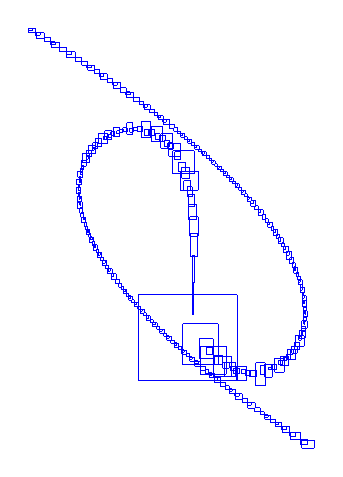
\begin{tikzpicture}[scale=4]
\draw[color=blue,line width=.1mm] (0.34823367733799204,-0.6256262823436587) --(0.3874643895035824,-0.6256262823436587);
\draw[color=blue,line width=.1mm] (0.34823367733799204,-0.6256262823436587) --(0.34823367733799204,-0.6000275732795886);
\draw[color=blue,line width=.1mm] (0.34823367733799204,-0.6000275732795886) --(0.3874643895035824,-0.6000275732795886);
\draw[color=blue,line width=.1mm] (0.3874643895035824,-0.6256262823436587) --(0.3874643895035824,-0.6000275732795886);
%\draw[color=white,line width=.2mm] (0.36790586580393153,-0.6127519155533838) --(0.3871959816973888,-0.62528770074817);
\draw[color=blue,line width=.1mm] (0.34368220063056126,-0.6128897585640191) --(0.36801488751093187,-0.6128897585640191);
\draw[color=blue,line width=.1mm] (0.34368220063056126,-0.6128897585640191) --(0.34368220063056126,-0.5969476393856569);
\draw[color=blue,line width=.1mm] (0.34368220063056126,-0.5969476393856569) --(0.36801488751093187,-0.5969476393856569);
\draw[color=blue,line width=.1mm] (0.36801488751093187,-0.6128897585640191) --(0.36801488751093187,-0.5969476393856569);
%\draw[color=white,line width=.2mm] (0.3438040468764289,-0.5970691106357413) --(0.36790586580393153,-0.6127519155533838);
\draw[color=blue,line width=.1mm] (0.3127444740308391,-0.5985829861920631) --(0.3445191986898834,-0.5985829861920631);
\draw[color=blue,line width=.1mm] (0.3127444740308391,-0.5985829861920631) --(0.3127444740308391,-0.5762335007339554);
\draw[color=blue,line width=.1mm] (0.3127444740308391,-0.5762335007339554) --(0.3445191986898834,-0.5762335007339554);
\draw[color=blue,line width=.1mm] (0.3445191986898834,-0.5985829861920631) --(0.3445191986898834,-0.5762335007339554);
%\draw[color=white,line width=.2mm] (0.3288393796968316,-0.5871384658838326) --(0.3438040468764289,-0.5970691106357413);
\draw[color=blue,line width=.1mm] (0.3100639433151495,-0.5872265584822126) --(0.32893176154637827,-0.5872265584822126);
\draw[color=blue,line width=.1mm] (0.3100639433151495,-0.5872265584822126) --(0.3100639433151495,-0.57460808360163);
\draw[color=blue,line width=.1mm] (0.3100639433151495,-0.57460808360163) --(0.32893176154637827,-0.57460808360163);
\draw[color=blue,line width=.1mm] (0.32893176154637827,-0.5872265584822126) --(0.32893176154637827,-0.57460808360163);
%\draw[color=white,line width=.2mm] (0.310120687801581,-0.574742318235947) --(0.3288393796968316,-0.5871384658838326);
\draw[color=blue,line width=.1mm] (0.2857802190516058,-0.5762351052748349) --(0.3108454654389906,-0.5762351052748349);
\draw[color=blue,line width=.1mm] (0.2857802190516058,-0.5762351052748349) --(0.2857802190516058,-0.5580295713938617);
\draw[color=blue,line width=.1mm] (0.2857802190516058,-0.5580295713938617) --(0.3108454654389906,-0.5580295713938617);
\draw[color=blue,line width=.1mm] (0.3108454654389906,-0.5762351052748349) --(0.3108454654389906,-0.5580295713938617);
%\draw[color=white,line width=.2mm] (0.2985222982870951,-0.5668664150549613) --(0.310120687801581,-0.574742318235947);
\draw[color=blue,line width=.1mm] (0.2838321585751084,-0.5671055042193167) --(0.2987761068526135,-0.5671055042193167);
\draw[color=blue,line width=.1mm] (0.2838321585751084,-0.5671055042193167) --(0.2838321585751084,-0.5567052106788744);
\draw[color=blue,line width=.1mm] (0.2838321585751084,-0.5567052106788744) --(0.2987761068526135,-0.5567052106788744);
\draw[color=blue,line width=.1mm] (0.2987761068526135,-0.5671055042193167) --(0.2987761068526135,-0.5567052106788744);
%\draw[color=white,line width=.2mm] (0.2839879525811337,-0.5570679567691471) --(0.2985222982870951,-0.5668664150549613);
\draw[color=blue,line width=.1mm] (0.26520955102522686,-0.5580195095783679) --(0.2844574957248272,-0.5580195095783679);
\draw[color=blue,line width=.1mm] (0.26520955102522686,-0.5580195095783679) --(0.26520955102522686,-0.5440433899450695);
\draw[color=blue,line width=.1mm] (0.26520955102522686,-0.5440433899450695) --(0.2844574957248272,-0.5440433899450695);
\draw[color=blue,line width=.1mm] (0.2844574957248272,-0.5580195095783679) --(0.2844574957248272,-0.5440433899450695);
%\draw[color=white,line width=.2mm] (0.27496927969354307,-0.5508624693089709) --(0.2839879525811337,-0.5570679567691471);
\draw[color=blue,line width=.1mm] (0.2635700368200267,-0.5510170437393652) --(0.27513548830117346,-0.5510170437393652);
\draw[color=blue,line width=.1mm] (0.2635700368200267,-0.5510170437393652) --(0.2635700368200267,-0.5429014023740718);
\draw[color=blue,line width=.1mm] (0.2635700368200267,-0.5429014023740718) --(0.27513548830117346,-0.5429014023740718);
\draw[color=blue,line width=.1mm] (0.27513548830117346,-0.5510170437393652) --(0.27513548830117346,-0.5429014023740718);
%\draw[color=white,line width=.2mm] (0.26367205335130534,-0.5431354738028413) --(0.27496927969354307,-0.5508624693089709);
\draw[color=blue,line width=.1mm] (0.24933983242033037,-0.5434804051927405) --(0.2638232788066239,-0.5434804051927405);
\draw[color=blue,line width=.1mm] (0.24933983242033037,-0.5434804051927405) --(0.24933983242033037,-0.5332044482655239);
\draw[color=blue,line width=.1mm] (0.24933983242033037,-0.5332044482655239) --(0.2638232788066239,-0.5332044482655239);
\draw[color=blue,line width=.1mm] (0.2638232788066239,-0.5434804051927405) --(0.2638232788066239,-0.5332044482655239);
%\draw[color=white,line width=.2mm] (0.24958627383149226,-0.5334327628306031) --(0.26367205335130534,-0.5431354738028413);
\draw[color=blue,line width=.1mm] (0.23128584215378586,-0.5344814275949898) --(0.250123568974279,-0.5344814275949898);
\draw[color=blue,line width=.1mm] (0.23128584215378586,-0.5344814275949898) --(0.23128584215378586,-0.5204442481108413);
\draw[color=blue,line width=.1mm] (0.23128584215378586,-0.5204442481108413) --(0.250123568974279,-0.5204442481108413);
\draw[color=blue,line width=.1mm] (0.250123568974279,-0.5344814275949898) --(0.250123568974279,-0.5204442481108413);
%\draw[color=white,line width=.2mm] (0.24085857539931832,-0.5272764022033192) --(0.24958627383149226,-0.5334327628306031);
\draw[color=blue,line width=.1mm] (0.2297612074971139,-0.5275021312525733) --(0.24110636774906288,-0.5275021312525733);
\draw[color=blue,line width=.1mm] (0.2297612074971139,-0.5275021312525733) --(0.2297612074971139,-0.5192832390283239);
\draw[color=blue,line width=.1mm] (0.2297612074971139,-0.5192832390283239) --(0.24110636774906288,-0.5192832390283239);
\draw[color=blue,line width=.1mm] (0.24110636774906288,-0.5275021312525733) --(0.24110636774906288,-0.5192832390283239);
%\draw[color=white,line width=.2mm] (0.22991329370987101,-0.519624308377142) --(0.24085857539931832,-0.5272764022033192);
\draw[color=blue,line width=.1mm] (0.21583155030273052,-0.5202260046968858) --(0.2302209802571932,-0.5202260046968858);
\draw[color=blue,line width=.1mm] (0.21583155030273052,-0.5202260046968858) --(0.21583155030273052,-0.5095674801884142);
\draw[color=blue,line width=.1mm] (0.21583155030273052,-0.5095674801884142) --(0.2302209802571932,-0.5095674801884142);
\draw[color=blue,line width=.1mm] (0.2302209802571932,-0.5202260046968858) --(0.2302209802571932,-0.5095674801884142);
%\draw[color=white,line width=.2mm] (0.216292789043981,-0.5099862055002681) --(0.22991329370987101,-0.519624308377142);
\draw[color=blue,line width=.1mm] (0.1989206993832345,-0.5104985916109763) --(0.2165617388611286,-0.5104985916109763);
\draw[color=blue,line width=.1mm] (0.1989206993832345,-0.5104985916109763) --(0.1989206993832345,-0.49751741926551407);
\draw[color=blue,line width=.1mm] (0.1989206993832345,-0.49751741926551407) --(0.2165617388611286,-0.49751741926551407);
\draw[color=blue,line width=.1mm] (0.2165617388611286,-0.5104985916109763) --(0.2165617388611286,-0.49751741926551407);
%\draw[color=white,line width=.2mm] (0.19931963170516218,-0.49787683260461146) --(0.216292789043981,-0.5099862055002681);
\draw[color=blue,line width=.1mm] (0.17743040249320463,-0.49887138279663734) --(0.19983529375736386,-0.49887138279663734);
\draw[color=blue,line width=.1mm] (0.17743040249320463,-0.49887138279663734) --(0.17743040249320463,-0.48192756076386534);
\draw[color=blue,line width=.1mm] (0.17743040249320463,-0.48192756076386534) --(0.19983529375736386,-0.48192756076386534);
\draw[color=blue,line width=.1mm] (0.19983529375736386,-0.49887138279663734) --(0.19983529375736386,-0.48192756076386534);
%\draw[color=white,line width=.2mm] (0.1887826539387326,-0.49022566902124487) --(0.19931963170516218,-0.49787683260461146);
\draw[color=blue,line width=.1mm] (0.17555032137045662,-0.4902973998575596) --(0.18883993449583675,-0.4902973998575596);
\draw[color=blue,line width=.1mm] (0.17555032137045662,-0.4902973998575596) --(0.17555032137045662,-0.48059456222447416);
\draw[color=blue,line width=.1mm] (0.17555032137045662,-0.48059456222447416) --(0.18883993449583675,-0.48059456222447416);
\draw[color=blue,line width=.1mm] (0.18883993449583675,-0.4902973998575596) --(0.18883993449583675,-0.48059456222447416);
%\draw[color=white,line width=.2mm] (0.17561779387091156,-0.48065476583061034) --(0.1887826539387326,-0.49022566902124487);
\draw[color=blue,line width=.1mm] (0.15872795031902032,-0.4812844951210189) --(0.17595019667788991,-0.4812844951210189);
\draw[color=blue,line width=.1mm] (0.15872795031902032,-0.4812844951210189) --(0.15872795031902032,-0.4681763148672524);
\draw[color=blue,line width=.1mm] (0.15872795031902032,-0.4681763148672524) --(0.17595019667788991,-0.4681763148672524);
\draw[color=blue,line width=.1mm] (0.17595019667788991,-0.4812844951210189) --(0.17595019667788991,-0.4681763148672524);
%\draw[color=white,line width=.2mm] (0.15922862567545798,-0.46861505654377733) --(0.17561779387091156,-0.48065476583061034);
\draw[color=blue,line width=.1mm] (0.13803675644667998,-0.4696265538196884) --(0.15976927451775588,-0.4696265538196884);
\draw[color=blue,line width=.1mm] (0.13803675644667998,-0.4696265538196884) --(0.13803675644667998,-0.4527377388704907);
\draw[color=blue,line width=.1mm] (0.13803675644667998,-0.4527377388704907) --(0.15976927451775588,-0.4527377388704907);
\draw[color=blue,line width=.1mm] (0.15976927451775588,-0.4696265538196884) --(0.15976927451775588,-0.4527377388704907);
%\draw[color=white,line width=.2mm] (0.14906008583491195,-0.4610066098542305) --(0.15922862567545798,-0.46861505654377733);
\draw[color=blue,line width=.1mm] (0.13629648318070486,-0.4610664112734856) --(0.14913025562615168,-0.4610664112734856);
\draw[color=blue,line width=.1mm] (0.13629648318070486,-0.4610664112734856) --(0.13629648318070486,-0.4514173555400237);
\draw[color=blue,line width=.1mm] (0.13629648318070486,-0.4514173555400237) --(0.14913025562615168,-0.4514173555400237);
\draw[color=blue,line width=.1mm] (0.14913025562615168,-0.4610664112734856) --(0.14913025562615168,-0.4514173555400237);
%\draw[color=white,line width=.2mm] (0.13633957777672112,-0.45150731741912464) --(0.14906008583491195,-0.4610066098542305);
\draw[color=blue,line width=.1mm] (0.11973744248348792,-0.4524901583821043) --(0.13687908651150335,-0.4524901583821043);
\draw[color=blue,line width=.1mm] (0.11973744248348792,-0.4524901583821043) --(0.11973744248348792,-0.4388269566582745);
\draw[color=blue,line width=.1mm] (0.11973744248348792,-0.4388269566582745) --(0.13687908651150335,-0.4388269566582745);
\draw[color=blue,line width=.1mm] (0.13687908651150335,-0.4524901583821043) --(0.13687908651150335,-0.4388269566582745);
%\draw[color=white,line width=.2mm] (0.1284642602339827,-0.4454880935777048) --(0.13633957777672112,-0.45150731741912464);
\draw[color=blue,line width=.1mm] (0.11847677202457146,-0.4456476893592732) --(0.12865351993094248,-0.4456476893592732);
\draw[color=blue,line width=.1mm] (0.11847677202457146,-0.4456476893592732) --(0.11847677202457146,-0.43775491128874605);
\draw[color=blue,line width=.1mm] (0.11847677202457146,-0.43775491128874605) --(0.12865351993094248,-0.43775491128874605);
\draw[color=blue,line width=.1mm] (0.12865351993094248,-0.4456476893592732) --(0.12865351993094248,-0.43775491128874605);
%\draw[color=white,line width=.2mm] (0.1185929390664284,-0.4379939192100018) --(0.1284642602339827,-0.4454880935777048);
\draw[color=blue,line width=.1mm] (0.10580317475431883,-0.4386158146988623) --(0.11893942905770899,-0.4386158146988623);
\draw[color=blue,line width=.1mm] (0.10580317475431883,-0.4386158146988623) --(0.10580317475431883,-0.4281157526164338);
\draw[color=blue,line width=.1mm] (0.10580317475431883,-0.4281157526164338) --(0.11893942905770899,-0.4281157526164338);
\draw[color=blue,line width=.1mm] (0.11893942905770899,-0.4386158146988623) --(0.11893942905770899,-0.4281157526164338);
%\draw[color=white,line width=.2mm] (0.10632260886609565,-0.42855219022015884) --(0.1185929390664284,-0.4379939192100018);
\draw[color=blue,line width=.1mm] (0.09059267522792958,-0.4290838641259495) --(0.10662693096350573,-0.4290838641259495);
\draw[color=blue,line width=.1mm] (0.09059267522792958,-0.4290838641259495) --(0.09059267522792958,-0.4163110797176512);
\draw[color=blue,line width=.1mm] (0.09059267522792958,-0.4163110797176512) --(0.10662693096350573,-0.4163110797176512);
\draw[color=blue,line width=.1mm] (0.10662693096350573,-0.4290838641259495) --(0.10662693096350573,-0.4163110797176512);
%\draw[color=white,line width=.2mm] (0.0910441092591467,-0.41668722761698024) --(0.10632260886609565,-0.42855219022015884);
\draw[color=blue,line width=.1mm] (0.07118468899899762,-0.41771741508624904) --(0.09162768697753217,-0.41771741508624904);
\draw[color=blue,line width=.1mm] (0.07118468899899762,-0.41771741508624904) --(0.07118468899899762,-0.40101033656161666);
\draw[color=blue,line width=.1mm] (0.07118468899899762,-0.40101033656161666) --(0.09162768697753217,-0.40101033656161666);
\draw[color=blue,line width=.1mm] (0.09162768697753217,-0.41771741508624904) --(0.09162768697753217,-0.40101033656161666);
%\draw[color=white,line width=.2mm] (0.08157569475043346,-0.4091875743257603) --(0.0910441092591467,-0.41668722761698024);
\draw[color=blue,line width=.1mm] (0.06968313158574736,-0.4092486905476238) --(0.0816513403391348,-0.4092486905476238);
\draw[color=blue,line width=.1mm] (0.06968313158574736,-0.4092486905476238) --(0.06968313158574736,-0.3997329496534934);
\draw[color=blue,line width=.1mm] (0.06968313158574736,-0.3997329496534934) --(0.0816513403391348,-0.3997329496534934);
\draw[color=blue,line width=.1mm] (0.0816513403391348,-0.4092486905476238) --(0.0816513403391348,-0.3997329496534934);
%\draw[color=white,line width=.2mm] (0.06972959055859707,-0.3998243246584348) --(0.08157569475043346,-0.4091875743257603);
\draw[color=blue,line width=.1mm] (0.05416252806101971,-0.4008271045466626) --(0.07031369207910307,-0.4008271045466626);
\draw[color=blue,line width=.1mm] (0.05416252806101971,-0.4008271045466626) --(0.05416252806101971,-0.3872949564691607);
\draw[color=blue,line width=.1mm] (0.05416252806101971,-0.3872949564691607) --(0.07031369207910307,-0.3872949564691607);
\draw[color=blue,line width=.1mm] (0.07031369207910307,-0.4008271045466626) --(0.07031369207910307,-0.3872949564691607);
%\draw[color=white,line width=.2mm] (0.06240698125651434,-0.3938896509764771) --(0.06972959055859707,-0.3998243246584348);
\draw[color=blue,line width=.1mm] (0.05309859713139074,-0.39405332606571336) --(0.06261181206042009,-0.39405332606571336);
\draw[color=blue,line width=.1mm] (0.05309859713139074,-0.39405332606571336) --(0.05309859713139074,-0.38625786445942084);
\draw[color=blue,line width=.1mm] (0.05309859713139074,-0.38625786445942084) --(0.06261181206042009,-0.38625786445942084);
\draw[color=blue,line width=.1mm] (0.06261181206042009,-0.39405332606571336) --(0.06261181206042009,-0.38625786445942084);
%\draw[color=white,line width=.2mm] (0.053224322848192784,-0.3865013216874107) --(0.06240698125651434,-0.3938896509764771);
\draw[color=blue,line width=.1mm] (0.041257322485488544,-0.387136208074577) --(0.053600104201631325,-0.387136208074577);
\draw[color=blue,line width=.1mm] (0.041257322485488544,-0.387136208074577) --(0.041257322485488544,-0.3767430203798598);
\draw[color=blue,line width=.1mm] (0.041257322485488544,-0.3767430203798598) --(0.053600104201631325,-0.3767430203798598);
\draw[color=blue,line width=.1mm] (0.053600104201631325,-0.387136208074577) --(0.053600104201631325,-0.3767430203798598);
%\draw[color=white,line width=.2mm] (0.041820638564264344,-0.3771914821578142) --(0.053224322848192784,-0.3865013216874107);
\draw[color=blue,line width=.1mm] (0.027140372049581175,-0.37773458525574766) --(0.04215110434841449,-0.37773458525574766);
\draw[color=blue,line width=.1mm] (0.027140372049581175,-0.37773458525574766) --(0.027140372049581175,-0.36510424755200743);
\draw[color=blue,line width=.1mm] (0.027140372049581175,-0.36510424755200743) --(0.04215110434841449,-0.36510424755200743);
\draw[color=blue,line width=.1mm] (0.04215110434841449,-0.37773458525574766) --(0.04215110434841449,-0.36510424755200743);
%\draw[color=white,line width=.2mm] (0.027630565791938712,-0.36549104206523536) --(0.041820638564264344,-0.3771914821578142);
\draw[color=blue,line width=.1mm] (0.009065517355454477,-0.36654307331149755) --(0.028264915119623157,-0.36654307331149755);
\draw[color=blue,line width=.1mm] (0.009065517355454477,-0.36654307331149755) --(0.009065517355454477,-0.34999869410489043);
\draw[color=blue,line width=.1mm] (0.009065517355454477,-0.34999869410489043) --(0.028264915119623157,-0.34999869410489043);
\draw[color=blue,line width=.1mm] (0.028264915119623157,-0.36654307331149755) --(0.028264915119623157,-0.34999869410489043);
%\draw[color=white,line width=.2mm] (0.018849448510060537,-0.3580938028157492) --(0.027630565791938712,-0.36549104206523536);
\draw[color=blue,line width=.1mm] (0.0078112310650405685,-0.3581563672731393) --(0.018931447229312847,-0.3581563672731393);
\draw[color=blue,line width=.1mm] (0.0078112310650405685,-0.3581563672731393) --(0.0078112310650405685,-0.34876573425829366);
\draw[color=blue,line width=.1mm] (0.0078112310650405685,-0.34876573425829366) --(0.018931447229312847,-0.34876573425829366);
\draw[color=blue,line width=.1mm] (0.018931447229312847,-0.3581563672731393) --(0.018931447229312847,-0.34876573425829366);
%\draw[color=white,line width=.2mm] (0.00786159360678376,-0.3488586100461525) --(0.018849448510060537,-0.3580938028157492);
\draw[color=blue,line width=.1mm] (-0.006700275171848579,-0.34988297291538883) --(0.00849774759558718,-0.34988297291538883);
\draw[color=blue,line width=.1mm] (-0.006700275171848579,-0.34988297291538883) --(-0.006700275171848579,-0.33646832103232127);
\draw[color=blue,line width=.1mm] (-0.006700275171848579,-0.33646832103232127) --(0.00849774759558718,-0.33646832103232127);
\draw[color=blue,line width=.1mm] (0.00849774759558718,-0.34988297291538883) --(0.00849774759558718,-0.33646832103232127);
%\draw[color=white,line width=.2mm] (0.0010826349561958901,-0.3430036171652662) --(0.00786159360678376,-0.3488586100461525);
\draw[color=blue,line width=.1mm] (-0.007559936032046669,-0.34317182581086664) --(0.0013056402344972704,-0.34317182581086664);
\draw[color=blue,line width=.1mm] (-0.007559936032046669,-0.34317182581086664) --(-0.007559936032046669,-0.33546677374776473);
\draw[color=blue,line width=.1mm] (-0.007559936032046669,-0.33546677374776473) --(0.0013056402344972704,-0.33546677374776473);
\draw[color=blue,line width=.1mm] (0.0013056402344972704,-0.34317182581086664) --(0.0013056402344972704,-0.33546677374776473);
%\draw[color=white,line width=.2mm] (-0.0074230534065579295,-0.335715003406538) --(0.0010826349561958901,-0.3430036171652662);
\draw[color=blue,line width=.1mm] (-0.018343246791671458,-0.3360871006910139) --(-0.007216288273964507,-0.3360871006910139);
\draw[color=blue,line width=.1mm] (-0.018343246791671458,-0.3360871006910139) --(-0.018343246791671458,-0.32630621000434357);
\draw[color=blue,line width=.1mm] (-0.018343246791671458,-0.32630621000434357) --(-0.007216288273964507,-0.32630621000434357);
\draw[color=blue,line width=.1mm] (-0.007216288273964507,-0.3360871006910139) --(-0.007216288273964507,-0.32630621000434357);
%\draw[color=white,line width=.2mm] (-0.01800629626228543,-0.32655931512122444) --(-0.0074230534065579295,-0.335715003406538);
\draw[color=blue,line width=.1mm] (-0.03218609850751438,-0.32769374888824815) --(-0.01726918464715329,-0.32769374888824815);
\draw[color=blue,line width=.1mm] (-0.03218609850751438,-0.32769374888824815) --(-0.03218609850751438,-0.3141720179156778);
\draw[color=blue,line width=.1mm] (-0.03218609850751438,-0.3141720179156778) --(-0.01726918464715329,-0.3141720179156778);
\draw[color=blue,line width=.1mm] (-0.01726918464715329,-0.32769374888824815) --(-0.01726918464715329,-0.3141720179156778);
%\draw[color=white,line width=.2mm] (-0.02451664218589159,-0.32074296981354794) --(-0.01800629626228543,-0.32655931512122444);
\draw[color=blue,line width=.1mm] (-0.03291168480203317,-0.3209922134894858) --(-0.0241772083695961,-0.3209922134894858);
\draw[color=blue,line width=.1mm] (-0.03291168480203317,-0.3209922134894858) --(-0.03291168480203317,-0.31315029545407547);
\draw[color=blue,line width=.1mm] (-0.03291168480203317,-0.31315029545407547) --(-0.0241772083695961,-0.31315029545407547);
\draw[color=blue,line width=.1mm] (-0.0241772083695961,-0.3209922134894858) --(-0.0241772083695961,-0.31315029545407547);
%\draw[color=white,line width=.2mm] (-0.03270334581357063,-0.3135166716842339) --(-0.02451664218589159,-0.32074296981354794);
\draw[color=blue,line width=.1mm] (-0.04323502828230221,-0.3138901927875577) --(-0.0324892466484157,-0.3138901927875577);
\draw[color=blue,line width=.1mm] (-0.04323502828230221,-0.3138901927875577) --(-0.04323502828230221,-0.30418396083293375);
\draw[color=blue,line width=.1mm] (-0.04323502828230221,-0.30418396083293375) --(-0.0324892466484157,-0.30418396083293375);
\draw[color=blue,line width=.1mm] (-0.0324892466484157,-0.3138901927875577) --(-0.0324892466484157,-0.30418396083293375);
%\draw[color=white,line width=.2mm] (-0.0428861259918367,-0.30443909669044433) --(-0.03270334581357063,-0.3135166716842339);
\draw[color=blue,line width=.1mm] (-0.05660024392771489,-0.3055791410319779) --(-0.04212189056623216,-0.3055791410319779);
\draw[color=blue,line width=.1mm] (-0.05660024392771489,-0.3055791410319779) --(-0.05660024392771489,-0.29214285186250155);
\draw[color=blue,line width=.1mm] (-0.05660024392771489,-0.29214285186250155) --(-0.04212189056623216,-0.29214285186250155);
\draw[color=blue,line width=.1mm] (-0.04212189056623216,-0.3055791410319779) --(-0.04212189056623216,-0.29214285186250155);
%\draw[color=white,line width=.2mm] (-0.04914233104205923,-0.2986719726626166) --(-0.0428861259918367,-0.30443909669044433);
\draw[color=blue,line width=.1mm] (-0.057229619028487985,-0.29892376797806514) --(-0.04878979054684639,-0.29892376797806514);
\draw[color=blue,line width=.1mm] (-0.057229619028487985,-0.29892376797806514) --(-0.057229619028487985,-0.2911385221000253);
\draw[color=blue,line width=.1mm] (-0.057229619028487985,-0.2911385221000253) --(-0.04878979054684639,-0.2911385221000253);
\draw[color=blue,line width=.1mm] (-0.04878979054684639,-0.29892376797806514) --(-0.04878979054684639,-0.2911385221000253);
%\draw[color=white,line width=.2mm] (-0.057013234720060195,-0.2915070837299526) --(-0.04914233104205923,-0.2986719726626166);
\draw[color=blue,line width=.1mm] (-0.0671610532324774,-0.29188196365823893) --(-0.056791323574354284,-0.29188196365823893);
\draw[color=blue,line width=.1mm] (-0.0671610532324774,-0.29188196365823893) --(-0.0671610532324774,-0.28224931357938254);
\draw[color=blue,line width=.1mm] (-0.0671610532324774,-0.28224931357938254) --(-0.056791323574354284,-0.28224931357938254);
\draw[color=blue,line width=.1mm] (-0.056791323574354284,-0.29188196365823893) --(-0.056791323574354284,-0.28224931357938254);
%\draw[color=white,line width=.2mm] (-0.06679942031217355,-0.2825065319173645) --(-0.057013234720060195,-0.2915070837299526);
\draw[color=blue,line width=.1mm] (-0.08005408802697787,-0.2836510741337545) --(-0.06600701901758442,-0.2836510741337545);
\draw[color=blue,line width=.1mm] (-0.08005408802697787,-0.2836510741337545) --(-0.08005408802697787,-0.27030075834883543);
\draw[color=blue,line width=.1mm] (-0.08005408802697787,-0.27030075834883543) --(-0.06600701901758442,-0.27030075834883543);
\draw[color=blue,line width=.1mm] (-0.06600701901758442,-0.2836510741337545) --(-0.06600701901758442,-0.27030075834883543);
%\draw[color=white,line width=.2mm] (-0.0728037672441448,-0.27678814463693235) --(-0.06679942031217355,-0.2825065319173645);
\draw[color=blue,line width=.1mm] (-0.08058604375559018,-0.2770418367225348) --(-0.07243826451461875,-0.2770418367225348);
\draw[color=blue,line width=.1mm] (-0.08058604375559018,-0.2770418367225348) --(-0.08058604375559018,-0.2693142504147973);
\draw[color=blue,line width=.1mm] (-0.08058604375559018,-0.2693142504147973) --(-0.07243826451461875,-0.2693142504147973);
\draw[color=blue,line width=.1mm] (-0.07243826451461875,-0.2770418367225348) --(-0.07243826451461875,-0.2693142504147973);
%\draw[color=white,line width=.2mm] (-0.08036170267552419,-0.2696838920231721) --(-0.0728037672441448,-0.27678814463693235);
\draw[color=blue,line width=.1mm] (-0.09012990353994611,-0.2700600240148864) --(-0.08013147238716557,-0.2700600240148864);
\draw[color=blue,line width=.1mm] (-0.09012990353994611,-0.2700600240148864) --(-0.09012990353994611,-0.26050011367791137);
\draw[color=blue,line width=.1mm] (-0.09012990353994611,-0.26050011367791137) --(-0.08013147238716557,-0.26050011367791137);
\draw[color=blue,line width=.1mm] (-0.08013147238716557,-0.2700600240148864) --(-0.08013147238716557,-0.26050011367791137);
%\draw[color=white,line width=.2mm] (-0.08975471349081773,-0.26075944955207575) --(-0.08036170267552419,-0.2696838920231721);
\draw[color=blue,line width=.1mm] (-0.10255655122055592,-0.26190815345707275) --(-0.08893232566661587,-0.26190815345707275);
\draw[color=blue,line width=.1mm] (-0.10255655122055592,-0.26190815345707275) --(-0.10255655122055592,-0.24864309187195655);
\draw[color=blue,line width=.1mm] (-0.10255655122055592,-0.24864309187195655) --(-0.08893232566661587,-0.24864309187195655);
\draw[color=blue,line width=.1mm] (-0.08893232566661587,-0.26190815345707275) --(-0.08893232566661587,-0.24864309187195655);
%\draw[color=white,line width=.2mm] (-0.0955090818676149,-0.25508934767418645) --(-0.08975471349081773,-0.26075944955207575);
\draw[color=blue,line width=.1mm] (-0.10298932814956414,-0.2553449466210072) --(-0.09512978231694787,-0.2553449466210072);
\draw[color=blue,line width=.1mm] (-0.10298932814956414,-0.2553449466210072) --(-0.10298932814956414,-0.24767453525386324);
\draw[color=blue,line width=.1mm] (-0.10298932814956414,-0.24767453525386324) --(-0.09512978231694787,-0.24767453525386324);
\draw[color=blue,line width=.1mm] (-0.09512978231694787,-0.2553449466210072) --(-0.09512978231694787,-0.24767453525386324);
%\draw[color=white,line width=.2mm] (-0.10275651797346716,-0.2480451116977244) --(-0.0955090818676149,-0.25508934767418645);
\draw[color=blue,line width=.1mm] (-0.11214893475907181,-0.24842233947874517) --(-0.1025174321132831,-0.24842233947874517);
\draw[color=blue,line width=.1mm] (-0.11214893475907181,-0.24842233947874517) --(-0.11214893475907181,-0.23893459904520312);
\draw[color=blue,line width=.1mm] (-0.11214893475907181,-0.23893459904520312) --(-0.1025174321132831,-0.23893459904520312);
\draw[color=blue,line width=.1mm] (-0.1025174321132831,-0.24842233947874517) --(-0.1025174321132831,-0.23893459904520312);
%\draw[color=white,line width=.2mm] (-0.11175931341206442,-0.2391960670216733) --(-0.10275651797346716,-0.2480451116977244);
\draw[color=blue,line width=.1mm] (-0.12411450581508925,-0.24034845084000064) --(-0.1109050093212887,-0.24034845084000064);
\draw[color=blue,line width=.1mm] (-0.12411450581508925,-0.24034845084000064) --(-0.12411450581508925,-0.22716841996637324);
\draw[color=blue,line width=.1mm] (-0.12411450581508925,-0.22716841996637324) --(-0.1109050093212887,-0.22716841996637324);
\draw[color=blue,line width=.1mm] (-0.1109050093212887,-0.24034845084000064) --(-0.1109050093212887,-0.22716841996637324);
%\draw[color=white,line width=.2mm] (-0.11726527943968763,-0.2335739488672905) --(-0.11175931341206442,-0.2391960670216733);
\draw[color=blue,line width=.1mm] (-0.12444614080192622,-0.23383144855750268) --(-0.11687129144735735,-0.23383144855750268);
\draw[color=blue,line width=.1mm] (-0.12444614080192622,-0.23383144855750268) --(-0.12444614080192622,-0.2262179644864589);
\draw[color=blue,line width=.1mm] (-0.12444614080192622,-0.2262179644864589) --(-0.11687129144735735,-0.2262179644864589);
\draw[color=blue,line width=.1mm] (-0.11687129144735735,-0.23383144855750268) --(-0.11687129144735735,-0.2262179644864589);
%\draw[color=white,line width=.2mm] (-0.12420431420139358,-0.22658928700022074) --(-0.11726527943968763,-0.2335739488672905);
\draw[color=blue,line width=.1mm] (-0.13322435607916805,-0.22696739572800936) --(-0.12395580813246443,-0.22696739572800936);
\draw[color=blue,line width=.1mm] (-0.13322435607916805,-0.22696739572800936) --(-0.13322435607916805,-0.2175515728822421);
\draw[color=blue,line width=.1mm] (-0.13322435607916805,-0.2175515728822421) --(-0.12395580813246443,-0.2175515728822421);
\draw[color=blue,line width=.1mm] (-0.12395580813246443,-0.22696739572800936) --(-0.12395580813246443,-0.2175515728822421);
%\draw[color=white,line width=.2mm] (-0.13281938328297455,-0.2178151625036389) --(-0.12420431420139358,-0.22658928700022074);
\draw[color=blue,line width=.1mm] (-0.14473365379770686,-0.21897056285136898) --(-0.13193113473342666,-0.21897056285136898);
\draw[color=blue,line width=.1mm] (-0.14473365379770686,-0.21897056285136898) --(-0.14473365379770686,-0.20587593780850114);
\draw[color=blue,line width=.1mm] (-0.14473365379770686,-0.20587593780850114) --(-0.13193113473342666,-0.20587593780850114);
\draw[color=blue,line width=.1mm] (-0.13193113473342666,-0.21897056285136898) --(-0.13193113473342666,-0.20587593780850114);
%\draw[color=white,line width=.2mm] (-0.13807821520361255,-0.21224090041755642) --(-0.13281938328297455,-0.2178151625036389);
\draw[color=blue,line width=.1mm] (-0.14496198757079864,-0.21250026780630377) --(-0.137668600305563,-0.21250026780630377);
\draw[color=blue,line width=.1mm] (-0.14496198757079864,-0.21250026780630377) --(-0.14496198757079864,-0.20494375693537675);
\draw[color=blue,line width=.1mm] (-0.14496198757079864,-0.20494375693537675) --(-0.137668600305563,-0.20494375693537675);
\draw[color=blue,line width=.1mm] (-0.137668600305563,-0.21250026780630377) --(-0.137668600305563,-0.20494375693537675);
%\draw[color=white,line width=.2mm] (-0.14471056846981317,-0.20531557497278505) --(-0.13807821520361255,-0.21224090041755642);
\draw[color=blue,line width=.1mm] (-0.1533612082816977,-0.20569428083648558) --(-0.14445205144466272,-0.20569428083648558);
\draw[color=blue,line width=.1mm] (-0.1533612082816977,-0.20569428083648558) --(-0.1533612082816977,-0.19635049301244903);
\draw[color=blue,line width=.1mm] (-0.1533612082816977,-0.19635049301244903) --(-0.14445205144466272,-0.19635049301244903);
\draw[color=blue,line width=.1mm] (-0.14445205144466272,-0.20569428083648558) --(-0.14445205144466272,-0.19635049301244903);
%\draw[color=white,line width=.2mm] (-0.15293992132808723,-0.19661616348312733) --(-0.14471056846981317,-0.20531557497278505);
\draw[color=blue,line width=.1mm] (-0.164418509912523,-0.1977737032782891) --(-0.1520156107566641,-0.1977737032782891);
\draw[color=blue,line width=.1mm] (-0.164418509912523,-0.1977737032782891) --(-0.164418509912523,-0.18476555910347023);
\draw[color=blue,line width=.1mm] (-0.164418509912523,-0.18476555910347023) --(-0.1520156107566641,-0.18476555910347023);
\draw[color=blue,line width=.1mm] (-0.1520156107566641,-0.1977737032782891) --(-0.1520156107566641,-0.18476555910347023);
%\draw[color=white,line width=.2mm] (-0.15795257536392787,-0.19108983084660763) --(-0.15293992132808723,-0.19661616348312733);
\draw[color=blue,line width=.1mm] (-0.16454119746728535,-0.19135100064080562) --(-0.15752635193299935,-0.19135100064080562);
\draw[color=blue,line width=.1mm] (-0.16454119746728535,-0.19135100064080562) --(-0.16454119746728535,-0.183851850130976);
\draw[color=blue,line width=.1mm] (-0.16454119746728535,-0.183851850130976) --(-0.15752635193299935,-0.183851850130976);
\draw[color=blue,line width=.1mm] (-0.15752635193299935,-0.19135100064080562) --(-0.15752635193299935,-0.183851850130976);
%\draw[color=white,line width=.2mm] (-0.16427958329108885,-0.18422384081891768) --(-0.15795257536392787,-0.19108983084660763);
\draw[color=blue,line width=.1mm] (-0.17256334562859516,-0.18460277943551365) --(-0.16401044199898857,-0.18460277943551365);
\draw[color=blue,line width=.1mm] (-0.17256334562859516,-0.18460277943551365) --(-0.17256334562859516,-0.17533157329045526);
\draw[color=blue,line width=.1mm] (-0.17256334562859516,-0.17533157329045526) --(-0.16401044199898857,-0.17533157329045526);
\draw[color=blue,line width=.1mm] (-0.16401044199898857,-0.18460277943551365) --(-0.16401044199898857,-0.17533157329045526);
%\draw[color=white,line width=.2mm] (-0.17212474505473419,-0.17559924752702585) --(-0.16427958329108885,-0.18422384081891768);
\draw[color=blue,line width=.1mm] (-0.18317238203786348,-0.1767578003214719) --(-0.17116217987682705,-0.1767578003214719);
\draw[color=blue,line width=.1mm] (-0.18317238203786348,-0.1767578003214719) --(-0.18317238203786348,-0.163838026304408);
\draw[color=blue,line width=.1mm] (-0.18317238203786348,-0.163838026304408) --(-0.17116217987682705,-0.163838026304408);
\draw[color=blue,line width=.1mm] (-0.17116217987682705,-0.1767578003214719) --(-0.17116217987682705,-0.163838026304408);
%\draw[color=white,line width=.2mm] (-0.17689186363549456,-0.1701211495938717) --(-0.17212474505473419,-0.17559924752702585);
\draw[color=blue,line width=.1mm] (-0.1831869101780035,-0.17038401820439691) --(-0.17644801304147453,-0.17038401820439691);
\draw[color=blue,line width=.1mm] (-0.1831869101780035,-0.17038401820439691) --(-0.1831869101780035,-0.16294301074497713);
\draw[color=blue,line width=.1mm] (-0.1831869101780035,-0.16294301074497713) --(-0.17644801304147453,-0.16294301074497713);
\draw[color=blue,line width=.1mm] (-0.17644801304147453,-0.17038401820439691) --(-0.17644801304147453,-0.16294301074497713);
%\draw[color=white,line width=.2mm] (-0.18291447564861324,-0.16331476707650616) --(-0.17689186363549456,-0.1701211495938717);
\draw[color=blue,line width=.1mm] (-0.1908334253267106,-0.16369348051910365) --(-0.18263407975886486,-0.16369348051910365);
\draw[color=blue,line width=.1mm] (-0.1908334253267106,-0.16369348051910365) --(-0.1908334253267106,-0.1544958995272087);
\draw[color=blue,line width=.1mm] (-0.1908334253267106,-0.1544958995272087) --(-0.18263407975886486,-0.1544958995272087);
\draw[color=blue,line width=.1mm] (-0.18263407975886486,-0.16369348051910365) --(-0.18263407975886486,-0.1544958995272087);
%\draw[color=white,line width=.2mm] (-0.19037648392187395,-0.1547654573830888) --(-0.18291447564861324,-0.16331476707650616);
\draw[color=blue,line width=.1mm] (-0.200997358623612,-0.15592360775588904) --(-0.18937341851317258,-0.15592360775588904);
\draw[color=blue,line width=.1mm] (-0.200997358623612,-0.15592360775588904) --(-0.200997358623612,-0.1430950362231525);
\draw[color=blue,line width=.1mm] (-0.200997358623612,-0.1430950362231525) --(-0.18937341851317258,-0.1430950362231525);
\draw[color=blue,line width=.1mm] (-0.18937341851317258,-0.15592360775588904) --(-0.18937341851317258,-0.1430950362231525);
%\draw[color=white,line width=.2mm] (-0.19489839720186142,-0.14933616623803192) --(-0.19037648392187395,-0.1547654573830888);
\draw[color=blue,line width=.1mm] (-0.20090107372780683,-0.14960058513497176) --(-0.1944358731820167,-0.14960058513497176);
\draw[color=blue,line width=.1mm] (-0.20090107372780683,-0.14960058513497176) --(-0.20090107372780683,-0.1422189598797512);
\draw[color=blue,line width=.1mm] (-0.20090107372780683,-0.1422189598797512) --(-0.1944358731820167,-0.1422189598797512);
\draw[color=blue,line width=.1mm] (-0.1944358731820167,-0.14960058513497176) --(-0.1944358731820167,-0.1422189598797512);
%\draw[color=white,line width=.2mm] (-0.20061717661544662,-0.14258997778982657) --(-0.19489839720186142,-0.14933616623803192);
\draw[color=blue,line width=.1mm] (-0.20817290836576494,-0.14296790047864252) --(-0.20032488670413504,-0.14296790047864252);
\draw[color=blue,line width=.1mm] (-0.20817290836576494,-0.14296790047864252) --(-0.20817290836576494,-0.13384556070285672);
\draw[color=blue,line width=.1mm] (-0.20817290836576494,-0.13384556070285672) --(-0.20032488670413504,-0.13384556070285672);
\draw[color=blue,line width=.1mm] (-0.20032488670413504,-0.14296790047864252) --(-0.20032488670413504,-0.13384556070285672);
%\draw[color=white,line width=.2mm] (-0.20769658411080938,-0.1341168315191169) --(-0.20061717661544662,-0.14258997778982657);
\draw[color=blue,line width=.1mm] (-0.21789430800888207,-0.1352728323680974) --(-0.2066507510043912,-0.1352728323680974);
\draw[color=blue,line width=.1mm] (-0.21789430800888207,-0.1352728323680974) --(-0.21789430800888207,-0.12253938095720218);
\draw[color=blue,line width=.1mm] (-0.21789430800888207,-0.12253938095720218) --(-0.2066507510043912,-0.12253938095720218);
\draw[color=blue,line width=.1mm] (-0.2066507510043912,-0.1352728323680974) --(-0.2066507510043912,-0.12253938095720218);
%\draw[color=white,line width=.2mm] (-0.2119733160329886,-0.12873722535634438) --(-0.20769658411080938,-0.1341168315191169);
\draw[color=blue,line width=.1mm] (-0.21768445632001876,-0.1290029938573006) --(-0.21149105825130154,-0.1290029938573006);
\draw[color=blue,line width=.1mm] (-0.21768445632001876,-0.1290029938573006) --(-0.21768445632001876,-0.12168251414915895);
\draw[color=blue,line width=.1mm] (-0.21768445632001876,-0.12168251414915895) --(-0.21149105825130154,-0.12168251414915895);
\draw[color=blue,line width=.1mm] (-0.21149105825130154,-0.1290029938573006) --(-0.21149105825130154,-0.12168251414915895);
%\draw[color=white,line width=.2mm] (-0.21738844577529154,-0.12205217859653206) --(-0.2119733160329886,-0.12873722535634438);
\draw[color=blue,line width=.1mm] (-0.22494504507649127,-0.1227140247447038) --(-0.21678244843515004,-0.1227140247447038);
\draw[color=blue,line width=.1mm] (-0.22494504507649127,-0.1227140247447038) --(-0.22494504507649127,-0.11313182979392297);
\draw[color=blue,line width=.1mm] (-0.22494504507649127,-0.11313182979392297) --(-0.21678244843515004,-0.11313182979392297);
\draw[color=blue,line width=.1mm] (-0.21678244843515004,-0.1227140247447038) --(-0.21678244843515004,-0.11313182979392297);
%\draw[color=white,line width=.2mm] (-0.22403703340676925,-0.11363042022631703) --(-0.21738844577529154,-0.12205217859653206);
\draw[color=blue,line width=.1mm] (-0.23303448541432586,-0.11419377657001553) --(-0.22350355070543443,-0.11419377657001553);
\draw[color=blue,line width=.1mm] (-0.23303448541432586,-0.11419377657001553) --(-0.23303448541432586,-0.10261997228952771);
\draw[color=blue,line width=.1mm] (-0.23303448541432586,-0.10261997228952771) --(-0.22350355070543443,-0.10261997228952771);
\draw[color=blue,line width=.1mm] (-0.22350355070543443,-0.11419377657001553) --(-0.22350355070543443,-0.10261997228952771);
%\draw[color=white,line width=.2mm] (-0.23224351529287118,-0.10304875064373044) --(-0.22403703340676925,-0.11363042022631703);
\draw[color=blue,line width=.1mm] (-0.24384407994982302,-0.10413309898249618) --(-0.23121386633026395,-0.10413309898249618);
\draw[color=blue,line width=.1mm] (-0.24384407994982302,-0.10413309898249618) --(-0.24384407994982302,-0.08889401215092557);
\draw[color=blue,line width=.1mm] (-0.24384407994982302,-0.08889401215092557) --(-0.23121386633026395,-0.08889401215092557);
\draw[color=blue,line width=.1mm] (-0.23121386633026395,-0.10413309898249618) --(-0.23121386633026395,-0.08889401215092557);
%\draw[color=white,line width=.2mm] (-0.2422938768592605,-0.0897165197395871) --(-0.23224351529287118,-0.10304875064373044);
\draw[color=blue,line width=.1mm] (-0.2570730286769417,-0.09144962503692479) --(-0.24059295106589207,-0.09144962503692479);
\draw[color=blue,line width=.1mm] (-0.2570730286769417,-0.09144962503692479) --(-0.2570730286769417,-0.07156238227967517);
\draw[color=blue,line width=.1mm] (-0.2570730286769417,-0.07156238227967517) --(-0.24059295106589207,-0.07156238227967517);
\draw[color=blue,line width=.1mm] (-0.24059295106589207,-0.09144962503692479) --(-0.24059295106589207,-0.07156238227967517);
%\draw[color=white,line width=.2mm] (-0.24833976091406512,-0.08127078277554281) --(-0.2422938768592605,-0.0897165197395871);
\draw[color=blue,line width=.1mm] (-0.25605625180896474,-0.08137481195092507) --(-0.24812797822659938,-0.08137481195092507);
\draw[color=blue,line width=.1mm] (-0.25605625180896474,-0.08137481195092507) --(-0.25605625180896474,-0.07058591987527281);
\draw[color=blue,line width=.1mm] (-0.25605625180896474,-0.07058591987527281) --(-0.24812797822659938,-0.07058591987527281);
\draw[color=blue,line width=.1mm] (-0.24812797822659938,-0.08137481195092507) --(-0.24812797822659938,-0.07058591987527281);
%\draw[color=white,line width=.2mm] (-0.255926113100234,-0.07072888290539368) --(-0.24833976091406512,-0.08127078277554281);
\draw[color=blue,line width=.1mm] (-0.2676760611931594,-0.0724087811930137) --(-0.2541805079228278,-0.0724087811930137);
\draw[color=blue,line width=.1mm] (-0.2676760611931594,-0.0724087811930137) --(-0.2676760611931594,-0.05609866212290099);
\draw[color=blue,line width=.1mm] (-0.2676760611931594,-0.05609866212290099) --(-0.2541805079228278,-0.05609866212290099);
\draw[color=blue,line width=.1mm] (-0.2541805079228278,-0.0724087811930137) --(-0.2541805079228278,-0.05609866212290099);
%\draw[color=white,line width=.2mm] (-0.26042451561524355,-0.06403241558115447) --(-0.255926113100234,-0.07072888290539368);
\draw[color=blue,line width=.1mm] (-0.26650876106752225,-0.0643271414415646) --(-0.2598147860061694,-0.0643271414415646);
\draw[color=blue,line width=.1mm] (-0.26650876106752225,-0.0643271414415646) --(-0.26650876106752225,-0.055304653793965985);
\draw[color=blue,line width=.1mm] (-0.26650876106752225,-0.055304653793965985) --(-0.2598147860061694,-0.055304653793965985);
\draw[color=blue,line width=.1mm] (-0.2598147860061694,-0.0643271414415646) --(-0.2598147860061694,-0.055304653793965985);
%\draw[color=white,line width=.2mm] (-0.2661344503116282,-0.055700931909394666) --(-0.26042451561524355,-0.06403241558115447);
\draw[color=blue,line width=.1mm] (-0.27407885870481785,-0.05630399392063336) --(-0.26555534918727297,-0.05630399392063336);
\draw[color=blue,line width=.1mm] (-0.27407885870481785,-0.05630399392063336) --(-0.27407885870481785,-0.04477526891238594);
\draw[color=blue,line width=.1mm] (-0.27407885870481785,-0.04477526891238594) --(-0.26555534918727297,-0.04477526891238594);
\draw[color=blue,line width=.1mm] (-0.26555534918727297,-0.05630399392063336) --(-0.26555534918727297,-0.04477526891238594);
%\draw[color=white,line width=.2mm] (-0.27313513840341647,-0.04522988808652884) --(-0.2661344503116282,-0.055700931909394666);
\draw[color=blue,line width=.1mm] (-0.28457628554837455,-0.047076132483807716) --(-0.2710469789214959,-0.047076132483807716);
\draw[color=blue,line width=.1mm] (-0.28457628554837455,-0.047076132483807716) --(-0.28457628554837455,-0.030525358059703696);
\draw[color=blue,line width=.1mm] (-0.28457628554837455,-0.030525358059703696) --(-0.2710469789214959,-0.030525358059703696);
\draw[color=blue,line width=.1mm] (-0.2710469789214959,-0.047076132483807716) --(-0.2710469789214959,-0.030525358059703696);
%\draw[color=white,line width=.2mm] (-0.27721496215259794,-0.03857009701786476) --(-0.27313513840341647,-0.04522988808652884);
\draw[color=blue,line width=.1mm] (-0.28303970831777775,-0.03900779126197978) --(-0.2762570305437512,-0.03900779126197978);
\draw[color=blue,line width=.1mm] (-0.28303970831777775,-0.03900779126197978) --(-0.28303970831777775,-0.029721911955135343);
\draw[color=blue,line width=.1mm] (-0.28303970831777775,-0.029721911955135343) --(-0.2762570305437512,-0.029721911955135343);
\draw[color=blue,line width=.1mm] (-0.2762570305437512,-0.03900779126197978) --(-0.2762570305437512,-0.029721911955135343);
%\draw[color=white,line width=.2mm] (-0.2824516742864476,-0.03029944261063518) --(-0.27721496215259794,-0.03857009701786476);
\draw[color=blue,line width=.1mm] (-0.2898605607840156,-0.030896978427454733) --(-0.2818323762255179,-0.030896978427454733);
\draw[color=blue,line width=.1mm] (-0.2898605607840156,-0.030896978427454733) --(-0.2898605607840156,-0.019448479262910687);
\draw[color=blue,line width=.1mm] (-0.2898605607840156,-0.019448479262910687) --(-0.2818323762255179,-0.019448479262910687);
\draw[color=blue,line width=.1mm] (-0.2818323762255179,-0.030896978427454733) --(-0.2818323762255179,-0.019448479262910687);
%\draw[color=white,line width=.2mm] (-0.28885133435635924,-0.019908394885222593) --(-0.2824516742864476,-0.03029944261063518);
\draw[color=blue,line width=.1mm] (-0.2997311763307194,-0.02173923372940048) --(-0.2866153743803848,-0.02173923372940048);
\draw[color=blue,line width=.1mm] (-0.2997311763307194,-0.02173923372940048) --(-0.2997311763307194,-0.005300105906295401);
\draw[color=blue,line width=.1mm] (-0.2997311763307194,-0.005300105906295401) --(-0.2866153743803848,-0.005300105906295401);
\draw[color=blue,line width=.1mm] (-0.2866153743803848,-0.02173923372940048) --(-0.2866153743803848,-0.005300105906295401);
%\draw[color=white,line width=.2mm] (-0.2925344921902075,-0.013307688346451987) --(-0.28885133435635924,-0.019908394885222593);
\draw[color=blue,line width=.1mm] (-0.29791722565578116,-0.013750677130929227) --(-0.29150547471663035,-0.013750677130929227);
\draw[color=blue,line width=.1mm] (-0.29791722565578116,-0.013750677130929227) --(-0.29791722565578116,-0.004535460221859659);
\draw[color=blue,line width=.1mm] (-0.29791722565578116,-0.004535460221859659) --(-0.29150547471663035,-0.004535460221859659);
\draw[color=blue,line width=.1mm] (-0.29150547471663035,-0.013750677130929227) --(-0.29150547471663035,-0.004535460221859659);
%\draw[color=white,line width=.2mm] (-0.2972855532409244,-0.005106914806621238) --(-0.2925344921902075,-0.013307688346451987);
\draw[color=blue,line width=.1mm] (-0.30414631671779013,-0.005694207283817694) --(-0.2966239469682953,-0.005694207283817694);
\draw[color=blue,line width=.1mm] (-0.30414631671779013,-0.005694207283817694) --(-0.30414631671779013,0.005655205954531677);
\draw[color=blue,line width=.1mm] (-0.30414631671779013,0.005655205954531677) --(-0.2966239469682953,0.005655205954531677);
\draw[color=blue,line width=.1mm] (-0.2966239469682953,-0.005694207283817694) --(-0.2966239469682953,0.005655205954531677);
%\draw[color=white,line width=.2mm] (-0.3030681435715547,0.005191705514721313) --(-0.2972855532409244,-0.005106914806621238);
\draw[color=blue,line width=.1mm] (-0.3133721617615956,0.0033930702627934187) --(-0.3006802758010744,0.0033930702627934187);
\draw[color=blue,line width=.1mm] (-0.3133721617615956,0.0033930702627934187) --(-0.3133721617615956,0.019676779964176903);
\draw[color=blue,line width=.1mm] (-0.3133721617615956,0.019676779964176903) --(-0.3006802758010744,0.019676779964176903);
\draw[color=blue,line width=.1mm] (-0.3006802758010744,0.0033930702627934187) --(-0.3006802758010744,0.019676779964176903);
%\draw[color=white,line width=.2mm] (-0.3063440758743253,0.011722863315784812) --(-0.3030681435715547,0.005191705514721313);
\draw[color=blue,line width=.1mm] (-0.31127131596091284,0.011278213768411975) --(-0.30524437302316154,0.011278213768411975);
\draw[color=blue,line width=.1mm] (-0.31127131596091284,0.011278213768411975) --(-0.31127131596091284,0.02040005653808507);
\draw[color=blue,line width=.1mm] (-0.31127131596091284,0.02040005653808507) --(-0.30524437302316154,0.02040005653808507);
\draw[color=blue,line width=.1mm] (-0.30524437302316154,0.011278213768411975) --(-0.30524437302316154,0.02040005653808507);
%\draw[color=white,line width=.2mm] (-0.3105962515037316,0.019842039731544633) --(-0.3063440758743253,0.011722863315784812);
\draw[color=blue,line width=.1mm] (-0.3168943445756668,0.019270660680428486) --(-0.3098908975129234,0.019270660680428486);
\draw[color=blue,line width=.1mm] (-0.3168943445756668,0.019270660680428486) --(-0.3168943445756668,0.030497210847040046);
\draw[color=blue,line width=.1mm] (-0.3168943445756668,0.030497210847040046) --(-0.3098908975129234,0.030497210847040046);
\draw[color=blue,line width=.1mm] (-0.3098908975129234,0.019270660680428486) --(-0.3098908975129234,0.030497210847040046);
%\draw[color=white,line width=.2mm] (-0.31574487884991426,0.030032276744928026) --(-0.3105962515037316,0.019842039731544633);
\draw[color=blue,line width=.1mm] (-0.3254572928993677,0.02828325396072673) --(-0.31320097367220495,0.02828325396072673);
\draw[color=blue,line width=.1mm] (-0.3254572928993677,0.02828325396072673) --(-0.3254572928993677,0.04436275093135977);
\draw[color=blue,line width=.1mm] (-0.3254572928993677,0.04436275093135977) --(-0.31320097367220495,0.04436275093135977);
\draw[color=blue,line width=.1mm] (-0.31320097367220495,0.02828325396072673) --(-0.31320097367220495,0.04436275093135977);
%\draw[color=white,line width=.2mm] (-0.31860243719885684,0.036480984700427925) --(-0.31574487884991426,0.030032276744928026);
\draw[color=blue,line width=.1mm] (-0.32306199061270985,0.03603695301973881) --(-0.31742979231342855,0.03603695301973881);
\draw[color=blue,line width=.1mm] (-0.32306199061270985,0.03603695301973881) --(-0.32306199061270985,0.04504240030184543);
\draw[color=blue,line width=.1mm] (-0.32306199061270985,0.04504240030184543) --(-0.31742979231342855,0.04504240030184543);
\draw[color=blue,line width=.1mm] (-0.31742979231342855,0.03603695301973881) --(-0.31742979231342855,0.04504240030184543);
%\draw[color=white,line width=.2mm] (-0.32234215023267243,0.044503780190471076) --(-0.31860243719885684,0.036480984700427925);
\draw[color=blue,line width=.1mm] (-0.3280611506013954,0.043954885428710316) --(-0.3215926445298535,0.043954885428710316);
\draw[color=blue,line width=.1mm] (-0.3280611506013954,0.043954885428710316) --(-0.3280611506013954,0.05502946367271658);
\draw[color=blue,line width=.1mm] (-0.3280611506013954,0.05502946367271658) --(-0.3215926445298535,0.05502946367271658);
\draw[color=blue,line width=.1mm] (-0.3215926445298535,0.043954885428710316) --(-0.3215926445298535,0.05502946367271658);
%\draw[color=white,line width=.2mm] (-0.32683973394168325,0.05456565661385266) --(-0.32234215023267243,0.044503780190471076);
\draw[color=blue,line width=.1mm] (-0.33593929006587403,0.052886103866355734) --(-0.32413973981442085,0.052886103866355734);
\draw[color=blue,line width=.1mm] (-0.33593929006587403,0.052886103866355734) --(-0.33593929006587403,0.06870342381155514);
\draw[color=blue,line width=.1mm] (-0.33593929006587403,0.06870342381155514) --(-0.32413973981442085,0.06870342381155514);
\draw[color=blue,line width=.1mm] (-0.32413973981442085,0.052886103866355734) --(-0.32413973981442085,0.06870342381155514);
%\draw[color=white,line width=.2mm] (-0.32926823016463963,0.06091612541591117) --(-0.32683973394168325,0.05456565661385266);
\draw[color=blue,line width=.1mm] (-0.33324718077447163,0.06047529322999076) --(-0.32802211677435683,0.06047529322999076);
\draw[color=blue,line width=.1mm] (-0.33324718077447163,0.06047529322999076) --(-0.33324718077447163,0.06933681958211133);
\draw[color=blue,line width=.1mm] (-0.33324718077447163,0.06933681958211133) --(-0.32802211677435683,0.06933681958211133);
\draw[color=blue,line width=.1mm] (-0.32802211677435683,0.06047529322999076) --(-0.32802211677435683,0.06933681958211133);
%\draw[color=white,line width=.2mm] (-0.33248224334457516,0.06882432929046399) --(-0.32926823016463963,0.06091612541591117);
\draw[color=blue,line width=.1mm] (-0.3385526458015954,0.06788912971821562) --(-0.3309014486887315,0.06788912971821562);
\draw[color=blue,line width=.1mm] (-0.3385526458015954,0.06788912971821562) --(-0.3385526458015954,0.07958995884543699);
\draw[color=blue,line width=.1mm] (-0.3385526458015954,0.07958995884543699) --(-0.3309014486887315,0.07958995884543699);
\draw[color=blue,line width=.1mm] (-0.3309014486887315,0.06788912971821562) --(-0.3309014486887315,0.07958995884543699);
%\draw[color=white,line width=.2mm] (-0.3361858254510347,0.07874869503832323) --(-0.33248224334457516,0.06882432929046399);
\draw[color=blue,line width=.1mm] (-0.3426065326877819,0.077968029163038) --(-0.3347924395149989,0.077968029163038);
\draw[color=blue,line width=.1mm] (-0.3426065326877819,0.077968029163038) --(-0.3426065326877819,0.09189889656003156);
\draw[color=blue,line width=.1mm] (-0.3426065326877819,0.09189889656003156) --(-0.3347924395149989,0.09189889656003156);
\draw[color=blue,line width=.1mm] (-0.3347924395149989,0.077968029163038) --(-0.3347924395149989,0.09189889656003156);
%\draw[color=white,line width=.2mm] (-0.34054255591067656,0.09117870011556392) --(-0.3361858254510347,0.07874869503832323);
\draw[color=blue,line width=.1mm] (-0.3494978189372732,0.0897380861282862) --(-0.33784781576458317,0.0897380861282862);
\draw[color=blue,line width=.1mm] (-0.3494978189372732,0.0897380861282862) --(-0.3494978189372732,0.10811118659368261);
\draw[color=blue,line width=.1mm] (-0.3494978189372732,0.10811118659368261) --(-0.33784781576458317,0.10811118659368261);
\draw[color=blue,line width=.1mm] (-0.33784781576458317,0.0897380861282862) --(-0.33784781576458317,0.10811118659368261);
%\draw[color=white,line width=.2mm] (-0.342891762836206,0.09897112704868394) --(-0.34054255591067656,0.09117870011556392);
\draw[color=blue,line width=.1mm] (-0.3460893904494826,0.0988672181721994) --(-0.34254486765450043,0.0988672181721994);
\draw[color=blue,line width=.1mm] (-0.3460893904494826,0.0988672181721994) --(-0.3460893904494826,0.10881852318034352);
\draw[color=blue,line width=.1mm] (-0.3460893904494826,0.10881852318034352) --(-0.34254486765450043,0.10881852318034352);
\draw[color=blue,line width=.1mm] (-0.34254486765450043,0.0988672181721994) --(-0.34254486765450043,0.10881852318034352);
%\draw[color=white,line width=.2mm] (-0.3458762315721723,0.10870568986970082) --(-0.342891762836206,0.09897112704868394);
\draw[color=blue,line width=.1mm] (-0.35314972330033784,0.10738843523047817) --(-0.3431475114144618,0.10738843523047817);
\draw[color=blue,line width=.1mm] (-0.35314972330033784,0.10738843523047817) --(-0.35314972330033784,0.1221849398940145);
\draw[color=blue,line width=.1mm] (-0.35314972330033784,0.1221849398940145) --(-0.3431475114144618,0.1221849398940145);
\draw[color=blue,line width=.1mm] (-0.3431475114144618,0.10738843523047817) --(-0.3431475114144618,0.1221849398940145);
%\draw[color=white,line width=.2mm] (-0.3490639989799434,0.12088412289254563) --(-0.3458762315721723,0.10870568986970082);
\draw[color=blue,line width=.1mm] (-0.35619053395372247,0.1197854003041102) --(-0.34661881361704217,0.1197854003041102);
\draw[color=blue,line width=.1mm] (-0.35619053395372247,0.1197854003041102) --(-0.35619053395372247,0.13722542707562022);
\draw[color=blue,line width=.1mm] (-0.35619053395372247,0.13722542707562022) --(-0.34661881361704217,0.13722542707562022);
\draw[color=blue,line width=.1mm] (-0.34661881361704217,0.1197854003041102) --(-0.34661881361704217,0.13722542707562022);
%\draw[color=white,line width=.2mm] (-0.3525686864787045,0.13609375577050833) --(-0.3490639989799434,0.12088412289254563);
\draw[color=blue,line width=.1mm] (-0.3630632219513744,0.13415438632543367) --(-0.34786950644898285,0.13415438632543367);
\draw[color=blue,line width=.1mm] (-0.3630632219513744,0.13415438632543367) --(-0.3630632219513744,0.15715072685449552);
\draw[color=blue,line width=.1mm] (-0.3630632219513744,0.15715072685449552) --(-0.34786950644898285,0.15715072685449552);
\draw[color=blue,line width=.1mm] (-0.34786950644898285,0.13415438632543367) --(-0.34786950644898285,0.15715072685449552);
%\draw[color=white,line width=.2mm] (-0.35410592871301994,0.14555755005491497) --(-0.3525686864787045,0.13609375577050833);
\draw[color=blue,line width=.1mm] (-0.3564861196441791,0.14540735242317798) --(-0.35349649594856714,0.14540735242317798);
\draw[color=blue,line width=.1mm] (-0.3564861196441791,0.14540735242317798) --(-0.3564861196441791,0.15752263867889899);
\draw[color=blue,line width=.1mm] (-0.3564861196441791,0.15752263867889899) --(-0.35349649594856714,0.15752263867889899);
\draw[color=blue,line width=.1mm] (-0.35349649594856714,0.14540735242317798) --(-0.35349649594856714,0.15752263867889899);
%\draw[color=white,line width=.2mm] (-0.35611154522492383,0.15738534282482816) --(-0.35410592871301994,0.14555755005491497);
\draw[color=blue,line width=.1mm] (-0.36478836553570404,0.15570120211483532) --(-0.3513559019774297,0.15570120211483532);
\draw[color=blue,line width=.1mm] (-0.36478836553570404,0.15570120211483532) --(-0.36478836553570404,0.1740545888387374);
\draw[color=blue,line width=.1mm] (-0.36478836553570404,0.1740545888387374) --(-0.3513559019774297,0.1740545888387374);
\draw[color=blue,line width=.1mm] (-0.3513559019774297,0.15570120211483532) --(-0.3513559019774297,0.1740545888387374);
%\draw[color=white,line width=.2mm] (-0.35670109464190397,0.16469245874432908) --(-0.35611154522492383,0.15738534282482816);
\draw[color=blue,line width=.1mm] (-0.3587159792018541,0.16425329713741638) --(-0.3550134876581909,0.16425329713741638);
\draw[color=blue,line width=.1mm] (-0.3587159792018541,0.16425329713741638) --(-0.3587159792018541,0.17419965001239296);
\draw[color=blue,line width=.1mm] (-0.3587159792018541,0.17419965001239296) --(-0.3550134876581909,0.17419965001239296);
\draw[color=blue,line width=.1mm] (-0.3550134876581909,0.16425329713741638) --(-0.3550134876581909,0.17419965001239296);
%\draw[color=white,line width=.2mm] (-0.3576799145530952,0.17385375817545054) --(-0.35670109464190397,0.16469245874432908);
\draw[color=blue,line width=.1mm] (-0.36103538558405146,0.17335227211317547) --(-0.3561492435912953,0.17335227211317547);
\draw[color=blue,line width=.1mm] (-0.36103538558405146,0.17335227211317547) --(-0.36103538558405146,0.18592842918026295);
\draw[color=blue,line width=.1mm] (-0.36103538558405146,0.18592842918026295) --(-0.3561492435912953,0.18592842918026295);
\draw[color=blue,line width=.1mm] (-0.3561492435912953,0.17335227211317547) --(-0.3561492435912953,0.18592842918026295);
%\draw[color=white,line width=.2mm] (-0.3585409588723797,0.1852393062746251) --(-0.3576799145530952,0.17385375817545054);
\draw[color=blue,line width=.1mm] (-0.36662280577986794,0.1836822291855808) --(-0.3530984353081539,0.1836822291855808);
\draw[color=blue,line width=.1mm] (-0.36662280577986794,0.1836822291855808) --(-0.36662280577986794,0.20139953074009304);
\draw[color=blue,line width=.1mm] (-0.36662280577986794,0.20139953074009304) --(-0.3530984353081539,0.20139953074009304);
\draw[color=blue,line width=.1mm] (-0.3530984353081539,0.1836822291855808) --(-0.3530984353081539,0.20139953074009304);
%\draw[color=white,line width=.2mm] (-0.35830655183795457,0.19218195097693164) --(-0.3585409588723797,0.1852393062746251);
\draw[color=blue,line width=.1mm] (-0.3599394869515468,0.1915517096787078) --(-0.35576575287173323,0.1915517096787078);
\draw[color=blue,line width=.1mm] (-0.3599394869515468,0.1915517096787078) --(-0.3599394869515468,0.20133315282883976);
\draw[color=blue,line width=.1mm] (-0.3599394869515468,0.20133315282883976) --(-0.35576575287173323,0.20133315282883976);
\draw[color=blue,line width=.1mm] (-0.35576575287173323,0.1915517096787078) --(-0.35576575287173323,0.20133315282883976);
%\draw[color=white,line width=.2mm] (-0.35837979966384037,0.20093771602502336) --(-0.35830655183795457,0.19218195097693164);
\draw[color=blue,line width=.1mm] (-0.3608818517735926,0.20048221301091346) --(-0.3565719562597223,0.20048221301091346);
\draw[color=blue,line width=.1mm] (-0.3608818517735926,0.20048221301091346) --(-0.3608818517735926,0.21252145363520342);
\draw[color=blue,line width=.1mm] (-0.3608818517735926,0.21252145363520342) --(-0.3565719562597223,0.21252145363520342);
\draw[color=blue,line width=.1mm] (-0.3565719562597223,0.20048221301091346) --(-0.3565719562597223,0.21252145363520342);
%\draw[color=white,line width=.2mm] (-0.3581073064397738,0.21177915248753837) --(-0.35837979966384037,0.20093771602502336);
\draw[color=blue,line width=.1mm] (-0.36566015053819223,0.2099628121363) --(-0.35177114227832584,0.2099628121363);
\draw[color=blue,line width=.1mm] (-0.36566015053819223,0.2099628121363) --(-0.36566015053819223,0.22768038330869758);
\draw[color=blue,line width=.1mm] (-0.36566015053819223,0.22768038330869758) --(-0.35177114227832584,0.22768038330869758);
\draw[color=blue,line width=.1mm] (-0.35177114227832584,0.2099628121363) --(-0.35177114227832584,0.22768038330869758);
%\draw[color=white,line width=.2mm] (-0.35716715764599394,0.2183023135669524) --(-0.3581073064397738,0.21177915248753837);
\draw[color=blue,line width=.1mm] (-0.3587347990892893,0.21742834002150255) --(-0.3538077175895167,0.21742834002150255);
\draw[color=blue,line width=.1mm] (-0.3587347990892893,0.21742834002150255) --(-0.3587347990892893,0.22710859984879414);
\draw[color=blue,line width=.1mm] (-0.3587347990892893,0.22710859984879414) --(-0.3538077175895167,0.22710859984879414);
\draw[color=blue,line width=.1mm] (-0.3538077175895167,0.21742834002150255) --(-0.3538077175895167,0.22710859984879414);
%\draw[color=white,line width=.2mm] (-0.35636158492102726,0.2265721160784101) --(-0.35716715764599394,0.2183023135669524);
\draw[color=blue,line width=.1mm] (-0.3587980686763626,0.2259631649259184) --(-0.3535044901120568,0.2259631649259184);
\draw[color=blue,line width=.1mm] (-0.3587980686763626,0.2259631649259184) --(-0.3587980686763626,0.23776200383609947);
\draw[color=blue,line width=.1mm] (-0.3587980686763626,0.23776200383609947) --(-0.3535044901120568,0.23776200383609947);
\draw[color=blue,line width=.1mm] (-0.3535044901120568,0.2259631649259184) --(-0.3535044901120568,0.23776200383609947);
%\draw[color=white,line width=.2mm] (-0.3549996051699791,0.2367696390576216) --(-0.35636158492102726,0.2265721160784101);
\draw[color=blue,line width=.1mm] (-0.3622863435831664,0.2344240077706172) --(-0.3475138342129344,0.2344240077706172);
\draw[color=blue,line width=.1mm] (-0.3622863435831664,0.2344240077706172) --(-0.3622863435831664,0.252548396068637);
\draw[color=blue,line width=.1mm] (-0.3622863435831664,0.252548396068637) --(-0.3475138342129344,0.252548396068637);
\draw[color=blue,line width=.1mm] (-0.3475138342129344,0.2344240077706172) --(-0.3475138342129344,0.252548396068637);
%\draw[color=white,line width=.2mm] (-0.3534056135195709,0.2428152964825968) --(-0.3549996051699791,0.2367696390576216);
\draw[color=blue,line width=.1mm] (-0.3549273412447076,0.2416907081379983) --(-0.3492942451286365,0.2416907081379983);
\draw[color=blue,line width=.1mm] (-0.3549273412447076,0.2416907081379983) --(-0.3549273412447076,0.251215333951354);
\draw[color=blue,line width=.1mm] (-0.3549273412447076,0.251215333951354) --(-0.3492942451286365,0.251215333951354);
\draw[color=blue,line width=.1mm] (-0.3492942451286365,0.2416907081379983) --(-0.3492942451286365,0.251215333951354);
%\draw[color=white,line width=.2mm] (-0.35177342716225524,0.2505250469553319) --(-0.3534056135195709,0.2428152964825968);
\draw[color=blue,line width=.1mm] (-0.3557755771481418,0.2490408063933452) --(-0.3465740370603264,0.2490408063933452);
\draw[color=blue,line width=.1mm] (-0.3557755771481418,0.2490408063933452) --(-0.3557755771481418,0.2620951950995683);
\draw[color=blue,line width=.1mm] (-0.3557755771481418,0.2620951950995683) --(-0.3465740370603264,0.2620951950995683);
\draw[color=blue,line width=.1mm] (-0.3465740370603264,0.2490408063933452) --(-0.3465740370603264,0.2620951950995683);
%\draw[color=white,line width=.2mm] (-0.34917122891511737,0.2598713623636396) --(-0.35177342716225524,0.2505250469553319);
\draw[color=blue,line width=.1mm] (-0.3523786085854718,0.2585067705748881) --(-0.3433700310263285,0.2585067705748881);
\draw[color=blue,line width=.1mm] (-0.3523786085854718,0.2585067705748881) --(-0.3523786085854718,0.27331032814428197);
\draw[color=blue,line width=.1mm] (-0.3523786085854718,0.27331032814428197) --(-0.3433700310263285,0.27331032814428197);
\draw[color=blue,line width=.1mm] (-0.3433700310263285,0.2585067705748881) --(-0.3433700310263285,0.27331032814428197);
%\draw[color=white,line width=.2mm] (-0.3454697914201885,0.27128737627939215) --(-0.34917122891511737,0.2598713623636396);
\draw[color=blue,line width=.1mm] (-0.3514911126214546,0.26852674953465555) --(-0.336096571346582,0.26852674953465555);
\draw[color=blue,line width=.1mm] (-0.3514911126214546,0.26852674953465555) --(-0.3514911126214546,0.28916269272508305);
\draw[color=blue,line width=.1mm] (-0.3514911126214546,0.28916269272508305) --(-0.336096571346582,0.28916269272508305);
\draw[color=blue,line width=.1mm] (-0.336096571346582,0.26852674953465555) --(-0.336096571346582,0.28916269272508305);
%\draw[color=white,line width=.2mm] (-0.3399921349194161,0.2850058274800583) --(-0.3454697914201885,0.27128737627939215);
\draw[color=blue,line width=.1mm] (-0.34900368602429777,0.28026446050645315) --(-0.3260369490675654,0.28026446050645315);
\draw[color=blue,line width=.1mm] (-0.34900368602429777,0.28026446050645315) --(-0.34900368602429777,0.3083449087236775);
\draw[color=blue,line width=.1mm] (-0.34900368602429777,0.3083449087236775) --(-0.3260369490675654,0.3083449087236775);
\draw[color=blue,line width=.1mm] (-0.3260369490675654,0.28026446050645315) --(-0.3260369490675654,0.3083449087236775);
%\draw[color=white,line width=.2mm] (-0.33568958104485186,0.29292823138662955) --(-0.3399921349194161,0.2850058274800583);
\draw[color=blue,line width=.1mm] (-0.33605808468399584,0.29240752600490305) --(-0.3299384275871354,0.29240752600490305);
\draw[color=blue,line width=.1mm] (-0.33605808468399584,0.29240752600490305) --(-0.33605808468399584,0.30336948961085364);
\draw[color=blue,line width=.1mm] (-0.33605808468399584,0.30336948961085364) --(-0.3299384275871354,0.30336948961085364);
\draw[color=blue,line width=.1mm] (-0.3299384275871354,0.29240752600490305) --(-0.3299384275871354,0.30336948961085364);
%\draw[color=white,line width=.2mm] (-0.33027838963987594,0.30276635397291024) --(-0.33568958104485186,0.29292823138662955);
\draw[color=blue,line width=.1mm] (-0.33528241571477435,0.29956018665549206) --(-0.3195703273042646,0.29956018665549206);
\draw[color=blue,line width=.1mm] (-0.33528241571477435,0.29956018665549206) --(-0.33528241571477435,0.3192499825076652);
\draw[color=blue,line width=.1mm] (-0.33528241571477435,0.3192499825076652) --(-0.3195703273042646,0.3192499825076652);
\draw[color=blue,line width=.1mm] (-0.3195703273042646,0.29956018665549206) --(-0.3195703273042646,0.3192499825076652);
%\draw[color=white,line width=.2mm] (-0.3228080496844681,0.3144228196234506) --(-0.33027838963987594,0.30276635397291024);
\draw[color=blue,line width=.1mm] (-0.3300952691097669,0.309108401786078) --(-0.307723610345453,0.309108401786078);
\draw[color=blue,line width=.1mm] (-0.3300952691097669,0.309108401786078) --(-0.3300952691097669,0.33593305932940754);
\draw[color=blue,line width=.1mm] (-0.3300952691097669,0.33593305932940754) --(-0.307723610345453,0.33593305932940754);
\draw[color=blue,line width=.1mm] (-0.307723610345453,0.309108401786078) --(-0.307723610345453,0.33593305932940754);
%\draw[color=white,line width=.2mm] (-0.3174279630529525,0.3209767507498482) --(-0.3228080496844681,0.3144228196234506);
\draw[color=blue,line width=.1mm] (-0.3176500462349886,0.32043836155832317) --(-0.31046405753927864,0.32043836155832317);
\draw[color=blue,line width=.1mm] (-0.3176500462349886,0.32043836155832317) --(-0.3176500462349886,0.32972094834882804);
\draw[color=blue,line width=.1mm] (-0.3176500462349886,0.32972094834882804) --(-0.31046405753927864,0.32972094834882804);
\draw[color=blue,line width=.1mm] (-0.31046405753927864,0.32043836155832317) --(-0.31046405753927864,0.32972094834882804);
%\draw[color=white,line width=.2mm] (-0.3106896560681633,0.3291099758537621) --(-0.3174279630529525,0.3209767507498482);
\draw[color=blue,line width=.1mm] (-0.3145484513536646,0.32568353977762876) --(-0.2992257940079869,0.32568353977762876);
\draw[color=blue,line width=.1mm] (-0.3145484513536646,0.32568353977762876) --(-0.3145484513536646,0.34375094696656583);
\draw[color=blue,line width=.1mm] (-0.3145484513536646,0.34375094696656583) --(-0.2992257940079869,0.34375094696656583);
\draw[color=blue,line width=.1mm] (-0.2992257940079869,0.32568353977762876) --(-0.2992257940079869,0.34375094696656583);
%\draw[color=white,line width=.2mm] (-0.30172223429854667,0.3385905818037011) --(-0.3106896560681633,0.3291099758537621);
\draw[color=blue,line width=.1mm] (-0.30715375688541074,0.3330644736962392) --(-0.2862297087945915,0.3330644736962392);
\draw[color=blue,line width=.1mm] (-0.30715375688541074,0.3330644736962392) --(-0.30715375688541074,0.35765820028255685);
\draw[color=blue,line width=.1mm] (-0.30715375688541074,0.35765820028255685) --(-0.2862297087945915,0.35765820028255685);
\draw[color=blue,line width=.1mm] (-0.2862297087945915,0.3330644736962392) --(-0.2862297087945915,0.35765820028255685);
%\draw[color=white,line width=.2mm] (-0.28974467858014114,0.34933477787867134) --(-0.30172223429854667,0.3385905818037011);
\draw[color=blue,line width=.1mm] (-0.29698921968578357,0.34048321480492044) --(-0.26905307862092737,0.34048321480492044);
\draw[color=blue,line width=.1mm] (-0.29698921968578357,0.34048321480492044) --(-0.29698921968578357,0.37432231181861747);
\draw[color=blue,line width=.1mm] (-0.29698921968578357,0.37432231181861747) --(-0.26905307862092737,0.37432231181861747);
\draw[color=blue,line width=.1mm] (-0.26905307862092737,0.34048321480492044) --(-0.26905307862092737,0.37432231181861747);
%\draw[color=white,line width=.2mm] (-0.28154633525660905,0.3548303048150719) --(-0.28974467858014114,0.34933477787867134);
\draw[color=blue,line width=.1mm] (-0.28216209808469306,0.35348637682483885) --(-0.27045267378143056,0.35348637682483885);
\draw[color=blue,line width=.1mm] (-0.28216209808469306,0.35348637682483885) --(-0.28216209808469306,0.36270933414500095);
\draw[color=blue,line width=.1mm] (-0.28216209808469306,0.36270933414500095) --(-0.27045267378143056,0.36270933414500095);
\draw[color=blue,line width=.1mm] (-0.27045267378143056,0.35348637682483885) --(-0.27045267378143056,0.36270933414500095);
%\draw[color=white,line width=.2mm] (-0.27145582011525393,0.36188429089246044) --(-0.28154633525660905,0.3548303048150719);
\draw[color=blue,line width=.1mm] (-0.276805597419138,0.3532845771368362) --(-0.25460709707460827,0.3532845771368362);
\draw[color=blue,line width=.1mm] (-0.276805597419138,0.3532845771368362) --(-0.276805597419138,0.3818964125783883);
\draw[color=blue,line width=.1mm] (-0.276805597419138,0.3818964125783883) --(-0.25460709707460827,0.3818964125783883);
\draw[color=blue,line width=.1mm] (-0.25460709707460827,0.3532845771368362) --(-0.25460709707460827,0.3818964125783883);
%\draw[color=white,line width=.2mm] (-0.2646140282011457,0.3651013285669312) --(-0.27145582011525393,0.36188429089246044);
\draw[color=blue,line width=.1mm] (-0.2655416649144789,0.36194041591362874) --(-0.25478154622439236,0.36194041591362874);
\draw[color=blue,line width=.1mm] (-0.2655416649144789,0.36194041591362874) --(-0.2655416649144789,0.371514519417466);
\draw[color=blue,line width=.1mm] (-0.2655416649144789,0.371514519417466) --(-0.25478154622439236,0.371514519417466);
\draw[color=blue,line width=.1mm] (-0.25478154622439236,0.36194041591362874) --(-0.25478154622439236,0.371514519417466);
%\draw[color=white,line width=.2mm] (-0.25629310117109233,0.3695746400683661) --(-0.2646140282011457,0.3651013285669312);
\draw[color=blue,line width=.1mm] (-0.2576597554127995,0.36692032549436887) --(-0.24484767531820872,0.36692032549436887);
\draw[color=blue,line width=.1mm] (-0.2576597554127995,0.36692032549436887) --(-0.2576597554127995,0.3788658661473285);
\draw[color=blue,line width=.1mm] (-0.2576597554127995,0.3788658661473285) --(-0.24484767531820872,0.3788658661473285);
\draw[color=blue,line width=.1mm] (-0.24484767531820872,0.36692032549436887) --(-0.24484767531820872,0.3788658661473285);
%\draw[color=white,line width=.2mm] (-0.24568630410367345,0.37454031654966724) --(-0.25629310117109233,0.3695746400683661);
\draw[color=blue,line width=.1mm] (-0.2491105403758258,0.3652467076975962) --(-0.22969687590446775,0.3652467076975962);
\draw[color=blue,line width=.1mm] (-0.2491105403758258,0.3652467076975962) --(-0.2491105403758258,0.39274855147997084);
\draw[color=blue,line width=.1mm] (-0.2491105403758258,0.39274855147997084) --(-0.22969687590446775,0.39274855147997084);
\draw[color=blue,line width=.1mm] (-0.22969687590446775,0.3652467076975962) --(-0.22969687590446775,0.39274855147997084);
%\draw[color=white,line width=.2mm] (-0.23869817472435534,0.3763329765721453) --(-0.24568630410367345,0.37454031654966724);
\draw[color=blue,line width=.1mm] (-0.2395149494329827,0.37188439449385413) --(-0.22883947556669695,0.37188439449385413);
\draw[color=blue,line width=.1mm] (-0.2395149494329827,0.37188439449385413) --(-0.2395149494329827,0.38194495692589925);
\draw[color=blue,line width=.1mm] (-0.2395149494329827,0.38194495692589925) --(-0.22883947556669695,0.38194495692589925);
\draw[color=blue,line width=.1mm] (-0.22883947556669695,0.37188439449385413) --(-0.22883947556669695,0.38194495692589925);
%\draw[color=white,line width=.2mm] (-0.23017044138315262,0.37921494367751263) --(-0.23869817472435534,0.3763329765721453);
\draw[color=blue,line width=.1mm] (-0.23078058871805582,0.37668937512129935) --(-0.21904150045201562,0.37668937512129935);
\draw[color=blue,line width=.1mm] (-0.23078058871805582,0.37668937512129935) --(-0.23078058871805582,0.3863362000461567);
\draw[color=blue,line width=.1mm] (-0.23078058871805582,0.3863362000461567) --(-0.21904150045201562,0.3863362000461567);
\draw[color=blue,line width=.1mm] (-0.21904150045201562,0.37668937512129935) --(-0.21904150045201562,0.3863362000461567);
%\draw[color=white,line width=.2mm] (-0.21941590908798358,0.38222045876710387) --(-0.23017044138315262,0.37921494367751263);
\draw[color=blue,line width=.1mm] (-0.21997727772243306,0.37829020015026216) --(-0.2055348608249238,0.37829020015026216);
\draw[color=blue,line width=.1mm] (-0.21997727772243306,0.37829020015026216) --(-0.21997727772243306,0.39145305676622555);
\draw[color=blue,line width=.1mm] (-0.21997727772243306,0.39145305676622555) --(-0.2055348608249238,0.39145305676622555);
\draw[color=blue,line width=.1mm] (-0.2055348608249238,0.37829020015026216) --(-0.2055348608249238,0.39145305676622555);
%\draw[color=white,line width=.2mm] (-0.20587933707989514,0.3850481909668713) --(-0.21941590908798358,0.38222045876710387);
\draw[color=blue,line width=.1mm] (-0.20661543423602707,0.37040900501672375) --(-0.18833728213621653,0.37040900501672375);
\draw[color=blue,line width=.1mm] (-0.20661543423602707,0.37040900501672375) --(-0.20661543423602707,0.40740429940417605);
\draw[color=blue,line width=.1mm] (-0.20661543423602707,0.40740429940417605) --(-0.18833728213621653,0.40740429940417605);
\draw[color=blue,line width=.1mm] (-0.18833728213621653,0.37040900501672375) --(-0.18833728213621653,0.40740429940417605);
%\draw[color=white,line width=.2mm] (-0.19731889301993955,0.3847304789344324) --(-0.20587933707989514,0.3850481909668713);
\draw[color=blue,line width=.1mm] (-0.19769979859021738,0.37685717756588094) --(-0.18611529588717282,0.37685717756588094);
\draw[color=blue,line width=.1mm] (-0.19769979859021738,0.37685717756588094) --(-0.19769979859021738,0.3903068096629166);
\draw[color=blue,line width=.1mm] (-0.19769979859021738,0.3903068096629166) --(-0.18611529588717282,0.3903068096629166);
\draw[color=blue,line width=.1mm] (-0.18611529588717282,0.37685717756588094) --(-0.18611529588717282,0.3903068096629166);
%\draw[color=white,line width=.2mm] (-0.18673603464242017,0.3854752233492193) --(-0.19731889301993955,0.3847304789344324);
\draw[color=blue,line width=.1mm] (-0.18710021850392006,0.38181391933169573) --(-0.1729899276947348,0.38181391933169573);
\draw[color=blue,line width=.1mm] (-0.18710021850392006,0.38181391933169573) --(-0.18710021850392006,0.3915038975537092);
\draw[color=blue,line width=.1mm] (-0.18710021850392006,0.3915038975537092) --(-0.1729899276947348,0.3915038975537092);
\draw[color=blue,line width=.1mm] (-0.1729899276947348,0.38181391933169573) --(-0.1729899276947348,0.3915038975537092);
%\draw[color=white,line width=.2mm] (-0.17358341242579686,0.3855389501536108) --(-0.18673603464242017,0.3854752233492193);
\draw[color=blue,line width=.1mm] (-0.17453426773061564,0.3786445149309244) --(-0.15579870076833813,0.3786445149309244);
\draw[color=blue,line width=.1mm] (-0.17453426773061564,0.3786445149309244) --(-0.17453426773061564,0.3947243599833697);
\draw[color=blue,line width=.1mm] (-0.17453426773061564,0.3947243599833697) --(-0.15579870076833813,0.3947243599833697);
\draw[color=blue,line width=.1mm] (-0.15579870076833813,0.3786445149309244) --(-0.15579870076833813,0.3947243599833697);
%\draw[color=white,line width=.2mm] (-0.15734824263476369,0.38428101648705193) --(-0.17358341242579686,0.3855389501536108);
\draw[color=blue,line width=.1mm] (-0.1620047191396882,0.35992974973717023) --(-0.13098292436977524,0.35992974973717023);
\draw[color=blue,line width=.1mm] (-0.1620047191396882,0.35992974973717023) --(-0.1620047191396882,0.4129792238186604);
\draw[color=blue,line width=.1mm] (-0.1620047191396882,0.4129792238186604) --(-0.13098292436977524,0.4129792238186604);
\draw[color=blue,line width=.1mm] (-0.13098292436977524,0.35992974973717023) --(-0.13098292436977524,0.4129792238186604);
%\draw[color=white,line width=.2mm] (-0.14783555594583508,0.38053807839395) --(-0.15734824263476369,0.38428101648705193);
\draw[color=blue,line width=.1mm] (-0.14985163766193832,0.36635309135084904) --(-0.13445856908454257,0.36635309135084904);
\draw[color=blue,line width=.1mm] (-0.14985163766193832,0.36635309135084904) --(-0.14985163766193832,0.3873720138835248);
\draw[color=blue,line width=.1mm] (-0.14985163766193832,0.3873720138835248) --(-0.13445856908454257,0.3873720138835248);
\draw[color=blue,line width=.1mm] (-0.13445856908454257,0.36635309135084904) --(-0.13445856908454257,0.3873720138835248);
%\draw[color=white,line width=.2mm] (-0.13569574272246793,0.3774896876451215) --(-0.14783555594583508,0.38053807839395);
\draw[color=blue,line width=.1mm] (-0.13764444087005998,0.36746016739007753) --(-0.11779057537510837,0.36746016739007753);
\draw[color=blue,line width=.1mm] (-0.13764444087005998,0.36746016739007753) --(-0.13764444087005998,0.38567496472924684);
\draw[color=blue,line width=.1mm] (-0.13764444087005998,0.38567496472924684) --(-0.11779057537510837,0.38567496472924684);
\draw[color=blue,line width=.1mm] (-0.11779057537510837,0.36746016739007753) --(-0.11779057537510837,0.38567496472924684);
%\draw[color=white,line width=.2mm] (-0.12096623150591818,0.372482951131816) --(-0.13569574272246793,0.3774896876451215);
\draw[color=blue,line width=.1mm] (-0.1286243334980462,0.3474427416035044) --(-0.09260225624169821,0.3474427416035044);
\draw[color=blue,line width=.1mm] (-0.1286243334980462,0.3474427416035044) --(-0.1286243334980462,0.39620377662815853);
\draw[color=blue,line width=.1mm] (-0.1286243334980462,0.39620377662815853) --(-0.09260225624169821,0.39620377662815853);
\draw[color=blue,line width=.1mm] (-0.09260225624169821,0.3474427416035044) --(-0.09260225624169821,0.39620377662815853);
%\draw[color=white,line width=.2mm] (-0.11281950637482774,0.3669502281807782) --(-0.12096623150591818,0.372482951131816);
\draw[color=blue,line width=.1mm] (-0.11618656679950172,0.3531143383820647) --(-0.10011063906442823,0.3531143383820647);
\draw[color=blue,line width=.1mm] (-0.11618656679950172,0.3531143383820647) --(-0.11618656679950172,0.37193144717594734);
\draw[color=blue,line width=.1mm] (-0.11618656679950172,0.37193144717594734) --(-0.10011063906442823,0.37193144717594734);
\draw[color=blue,line width=.1mm] (-0.10011063906442823,0.3531143383820647) --(-0.10011063906442823,0.37193144717594734);
%\draw[color=white,line width=.2mm] (-0.10217674843196019,0.36123201438221203) --(-0.11281950637482774,0.3669502281807782);
\draw[color=blue,line width=.1mm] (-0.10476269924586583,0.34878176861342564) --(-0.08525915568500701,0.34878176861342564);
\draw[color=blue,line width=.1mm] (-0.10476269924586583,0.34878176861342564) --(-0.10476269924586583,0.3682063263865892);
\draw[color=blue,line width=.1mm] (-0.10476269924586583,0.3682063263865892) --(-0.08525915568500701,0.3682063263865892);
\draw[color=blue,line width=.1mm] (-0.08525915568500701,0.34878176861342564) --(-0.08525915568500701,0.3682063263865892);
%\draw[color=white,line width=.2mm] (-0.08947329764105012,0.35306146014956485) --(-0.10217674843196019,0.36123201438221203);
\draw[color=blue,line width=.1mm] (-0.09900777826000175,0.3271069905938194) --(-0.061227473296766935,0.3271069905938194);
\draw[color=blue,line width=.1mm] (-0.09900777826000175,0.3271069905938194) --(-0.09900777826000175,0.37294212452681597);
\draw[color=blue,line width=.1mm] (-0.09900777826000175,0.37294212452681597) --(-0.061227473296766935,0.37294212452681597);
\draw[color=blue,line width=.1mm] (-0.061227473296766935,0.3271069905938194) --(-0.061227473296766935,0.37294212452681597);
%\draw[color=white,line width=.2mm] (-0.082862293617457,0.3459385086860175) --(-0.08947329764105012,0.35306146014956485);
\draw[color=blue,line width=.1mm] (-0.08726696986718625,0.33119788729562866) --(-0.07127645846935511,0.33119788729562866);
\draw[color=blue,line width=.1mm] (-0.08726696986718625,0.33119788729562866) --(-0.08726696986718625,0.3501451121559411);
\draw[color=blue,line width=.1mm] (-0.08726696986718625,0.3501451121559411) --(-0.07127645846935511,0.3501451121559411);
\draw[color=blue,line width=.1mm] (-0.07127645846935511,0.33119788729562866) --(-0.07127645846935511,0.3501451121559411);
%\draw[color=white,line width=.2mm] (-0.07397912348288256,0.3380535522450767) --(-0.082862293617457,0.3459385086860175);
\draw[color=blue,line width=.1mm] (-0.0768266684628087,0.32391339929405855) --(-0.05890068103522014,0.32391339929405855);
\draw[color=blue,line width=.1mm] (-0.0768266684628087,0.32391339929405855) --(-0.0768266684628087,0.34368493933676997);
\draw[color=blue,line width=.1mm] (-0.0768266684628087,0.34368493933676997) --(-0.05890068103522014,0.34368493933676997);
\draw[color=blue,line width=.1mm] (-0.05890068103522014,0.32391339929405855) --(-0.05890068103522014,0.34368493933676997);
%\draw[color=white,line width=.2mm] (-0.063541124594092,0.3273690232738544) --(-0.07397912348288256,0.3380535522450767);
\draw[color=blue,line width=.1mm] (-0.07364522116772453,0.30151425035847984) --(-0.037400904733702486,0.30151425035847984);
\draw[color=blue,line width=.1mm] (-0.07364522116772453,0.30151425035847984) --(-0.07364522116772453,0.3431549113750521);
\draw[color=blue,line width=.1mm] (-0.07364522116772453,0.3431549113750521) --(-0.037400904733702486,0.3431549113750521);
\draw[color=blue,line width=.1mm] (-0.037400904733702486,0.30151425035847984) --(-0.037400904733702486,0.3431549113750521);
%\draw[color=white,line width=.2mm] (-0.05243972236477701,0.3118098808412073) --(-0.063541124594092,0.3273690232738544);
\draw[color=blue,line width=.1mm] (-0.054773111260127176,0.2900689866064626) --(-0.03532624828219776,0.2900689866064626);
\draw[color=blue,line width=.1mm] (-0.054773111260127176,0.2900689866064626) --(-0.054773111260127176,0.31484343048851443);
\draw[color=blue,line width=.1mm] (-0.054773111260127176,0.31484343048851443) --(-0.03532624828219776,0.31484343048851443);
\draw[color=blue,line width=.1mm] (-0.03532624828219776,0.2900689866064626) --(-0.03532624828219776,0.31484343048851443);
%\draw[color=white,line width=.2mm] (-0.039129988056507505,0.2919297416762712) --(-0.05243972236477701,0.3118098808412073);
\draw[color=blue,line width=.1mm] (-0.061116817769900654,0.24580886297017396) --(0.006235625348679032,0.24580886297017396);
\draw[color=blue,line width=.1mm] (-0.061116817769900654,0.24580886297017396) --(-0.061116817769900654,0.31889738131403983);
\draw[color=blue,line width=.1mm] (-0.061116817769900654,0.31889738131403983) --(0.006235625348679032,0.31889738131403983);
\draw[color=blue,line width=.1mm] (0.006235625348679032,0.24580886297017396) --(0.006235625348679032,0.31889738131403983);
%\draw[color=white,line width=.2mm] (-0.033835285256528694,0.2768402971264373) --(-0.039129988056507505,0.2919297416762712);
\draw[color=blue,line width=.1mm] (-0.0423252973771111,0.2516497778339698) --(-0.020787798893443947,0.2516497778339698);
\draw[color=blue,line width=.1mm] (-0.0423252973771111,0.2516497778339698) --(-0.0423252973771111,0.28142558022927633);
\draw[color=blue,line width=.1mm] (-0.0423252973771111,0.28142558022927633) --(-0.020787798893443947,0.28142558022927633);
\draw[color=blue,line width=.1mm] (-0.020787798893443947,0.2516497778339698) --(-0.020787798893443947,0.28142558022927633);
%\draw[color=white,line width=.2mm] (-0.0259960694321466,0.25912405328795085) --(-0.033835285256528694,0.2768402971264373);
\draw[color=blue,line width=.1mm] (-0.03210871063202384,0.23158906050860578) --(-0.0076755905072833155,0.23158906050860578);
\draw[color=blue,line width=.1mm] (-0.03210871063202384,0.23158906050860578) --(-0.03210871063202384,0.26619118952560866);
\draw[color=blue,line width=.1mm] (-0.03210871063202384,0.26619118952560866) --(-0.0076755905072833155,0.26619118952560866);
\draw[color=blue,line width=.1mm] (-0.0076755905072833155,0.23158906050860578) --(-0.0076755905072833155,0.26619118952560866);
%\draw[color=white,line width=.2mm] (-0.01763693152312403,0.23592571243780452) --(-0.0259960694321466,0.25912405328795085);
\draw[color=blue,line width=.1mm] (-0.03782251370451618,0.1924410326566978) --(0.018939536259647276,0.1924410326566978);
\draw[color=blue,line width=.1mm] (-0.03782251370451618,0.1924410326566978) --(-0.03782251370451618,0.2542031096338725);
\draw[color=blue,line width=.1mm] (-0.03782251370451618,0.2542031096338725) --(0.018939536259647276,0.2542031096338725);
\draw[color=blue,line width=.1mm] (0.018939536259647276,0.1924410326566978) --(0.018939536259647276,0.2542031096338725);
%\draw[color=white,line width=.2mm] (-0.015250148935355116,0.21955423282359668) --(-0.01763693152312403,0.23592571243780452);
\draw[color=blue,line width=.1mm] (-0.02578363126026303,0.19327134054822098) --(-0.004272856786836168,0.19327134054822098);
\draw[color=blue,line width=.1mm] (-0.02578363126026303,0.19327134054822098) --(-0.02578363126026303,0.22376591314298283);
\draw[color=blue,line width=.1mm] (-0.02578363126026303,0.22376591314298283) --(-0.004272856786836168,0.22376591314298283);
\draw[color=blue,line width=.1mm] (-0.004272856786836168,0.19327134054822098) --(-0.004272856786836168,0.22376591314298283);
%\draw[color=white,line width=.2mm] (-0.010734950392248447,0.20013642827473455) --(-0.015250148935355116,0.21955423282359668);
\draw[color=blue,line width=.1mm] (-0.015213663745763259,0.17278107120789518) --(0.0011485701565644565,0.17278107120789518);
\draw[color=blue,line width=.1mm] (-0.015213663745763259,0.17278107120789518) --(-0.015213663745763259,0.2041801356141821);
\draw[color=blue,line width=.1mm] (-0.015213663745763259,0.2041801356141821) --(0.0011485701565644565,0.2041801356141821);
\draw[color=blue,line width=.1mm] (0.0011485701565644565,0.17278107120789518) --(0.0011485701565644565,0.2041801356141821);
%\draw[color=white,line width=.2mm] (-0.0061500737123072234,0.17526243721306597) --(-0.010734950392248447,0.20013642827473455);
\draw[color=blue,line width=.1mm] (-0.012308491498101358,0.14026083838462017) --(0.008159939939519535,0.14026083838462017);
\draw[color=blue,line width=.1mm] (-0.012308491498101358,0.14026083838462017) --(-0.012308491498101358,0.18038515048601783);
\draw[color=blue,line width=.1mm] (-0.012308491498101358,0.18038515048601783) --(0.008159939939519535,0.18038515048601783);
\draw[color=blue,line width=.1mm] (0.008159939939519535,0.14026083838462017) --(0.008159939939519535,0.18038515048601783);
%\draw[color=white,line width=.2mm] (-0.0018759999780204033,0.14340432166764236) --(-0.0061500737123072234,0.17526243721306597);
\draw[color=blue,line width=.1mm] (-0.009850498640165593,0.09894973600724759) --(0.014574154045245681,0.09894973600724759);
\draw[color=blue,line width=.1mm] (-0.009850498640165593,0.09894973600724759) --(-0.009850498640165593,0.14947002418315086);
\draw[color=blue,line width=.1mm] (-0.009850498640165593,0.14947002418315086) --(0.014574154045245681,0.14947002418315086);
\draw[color=blue,line width=.1mm] (0.014574154045245681,0.09894973600724759) --(0.014574154045245681,0.14947002418315086);
%\draw[color=white,line width=.2mm] (0.0015786749263027751,0.10267187181084361) --(-0.0018759999780204033,0.14340432166764236);
\draw[color=blue,line width=.1mm] (-0.00773284789493811,0.046810423043379804) --(0.01886539945525545,0.046810423043379804);
\draw[color=blue,line width=.1mm] (-0.00773284789493811,0.046810423043379804) --(-0.00773284789493811,0.10914782529772284);
\draw[color=blue,line width=.1mm] (-0.00773284789493811,0.10914782529772284) --(0.01886539945525545,0.10914782529772284);
\draw[color=blue,line width=.1mm] (0.01886539945525545,0.046810423043379804) --(0.01886539945525545,0.10914782529772284);
%\draw[color=white,line width=.2mm] (0.0036910661709392474,0.05078430382485779) --(0.0015786749263027751,0.10267187181084361);
\draw[color=blue,line width=.1mm] (-0.004978176056835987,-0.018349841091238665) --(0.018404463426479882,-0.018349841091238665);
\draw[color=blue,line width=.1mm] (-0.004978176056835987,-0.018349841091238665) --(-0.004978176056835987,0.05638817188477446);
\draw[color=blue,line width=.1mm] (-0.004978176056835987,0.05638817188477446) --(0.018404463426479882,0.05638817188477446);
\draw[color=blue,line width=.1mm] (0.018404463426479882,-0.018349841091238665) --(0.018404463426479882,0.05638817188477446);
%\draw[color=white,line width=.2mm] (0.004276809611135531,-0.01491110358825988) --(0.0036910661709392474,0.05078430382485779);
\draw[color=blue,line width=.1mm] (0.0016483371485399856,-0.09828947524202261) --(0.00866938218433902,-0.09828947524202261);
\draw[color=blue,line width=.1mm] (0.0016483371485399856,-0.09828947524202261) --(0.0016483371485399856,-0.013254405396405794);
\draw[color=blue,line width=.1mm] (0.0016483371485399856,-0.013254405396405794) --(0.00866938218433902,-0.013254405396405794);
\draw[color=blue,line width=.1mm] (0.00866938218433902,-0.09828947524202261) --(0.00866938218433902,-0.013254405396405794);
%\draw[color=white,line width=.2mm] (0.004385945630946502,-0.09727286475781118) --(0.004276809611135531,-0.01491110358825988);
\draw[color=blue,line width=.1mm] (0.00030196167836183535,-0.2003228697594206) --(0.005900735603519565,-0.2003228697594206);
\draw[color=blue,line width=.1mm] (0.00030196167836183535,-0.2003228697594206) --(0.00030196167836183535,-0.09822615253682687);
\draw[color=blue,line width=.1mm] (0.00030196167836183535,-0.09822615253682687) --(0.005900735603519565,-0.09822615253682687);
\draw[color=blue,line width=.1mm] (0.005900735603519565,-0.2003228697594206) --(0.005900735603519565,-0.09822615253682687);
%\draw[color=white,line width=.2mm] (0.005370716418608002,-0.2000164828825746) --(0.004385945630946502,-0.09727286475781118);
\draw[color=blue,line width=.1mm] (-0.17026768264420764,-0.41059471900536837) --(0.1433771507529126,-0.41059471900536837);
\draw[color=blue,line width=.1mm] (-0.17026768264420764,-0.41059471900536837) --(-0.17026768264420764,-0.1391036291696054);
\draw[color=blue,line width=.1mm] (-0.17026768264420764,-0.1391036291696054) --(0.1433771507529126,-0.1391036291696054);
\draw[color=blue,line width=.1mm] (0.1433771507529126,-0.41059471900536837) --(0.1433771507529126,-0.1391036291696054);
%\draw[color=white,line width=.2mm] (0.021445860984428706,-0.25668601031467403) --(0.005370716418608002,-0.2000164828825746);
\draw[color=blue,line width=.1mm] (-0.02968209554182311,-0.3606520978171913) --(0.08262517998719643,-0.3606520978171913);
\draw[color=blue,line width=.1mm] (-0.02968209554182311,-0.3606520978171913) --(-0.02968209554182311,-0.2305285409927903);
\draw[color=blue,line width=.1mm] (-0.02968209554182311,-0.2305285409927903) --(0.08262517998719643,-0.2305285409927903);
\draw[color=blue,line width=.1mm] (0.08262517998719643,-0.3606520978171913) --(0.08262517998719643,-0.2305285409927903);
%\draw[color=white,line width=.2mm] (0.03707211404263725,-0.28822004779399385) --(0.021445860984428706,-0.25668601031467403);
\draw[color=blue,line width=.1mm] (0.023529931853298297,-0.3397696101109953) --(0.06788354373700564,-0.3397696101109953);
\draw[color=blue,line width=.1mm] (0.023529931853298297,-0.3397696101109953) --(0.023529931853298297,-0.27812559561603606);
\draw[color=blue,line width=.1mm] (0.023529931853298297,-0.27812559561603606) --(0.06788354373700564,-0.27812559561603606);
\draw[color=blue,line width=.1mm] (0.06788354373700564,-0.3397696101109953) --(0.06788354373700564,-0.27812559561603606);
%\draw[color=white,line width=.2mm] (0.048682541829673714,-0.3062544104202489) --(0.03707211404263725,-0.28822004779399385);
\draw[color=blue,line width=.1mm] (0.047180629267798056,-0.3297231043070097) --(0.0652619206136775,-0.3297231043070097);
\draw[color=blue,line width=.1mm] (0.047180629267798056,-0.3297231043070097) --(0.047180629267798056,-0.3049548189992093);
\draw[color=blue,line width=.1mm] (0.047180629267798056,-0.3049548189992093) --(0.0652619206136775,-0.3049548189992093);
\draw[color=blue,line width=.1mm] (0.0652619206136775,-0.3297231043070097) --(0.0652619206136775,-0.3049548189992093);
%\draw[color=white,line width=.2mm] (0.06281735027605177,-0.3289240555626426) --(0.048682541829673714,-0.3062544104202489);
\draw[color=blue,line width=.1mm] (0.026016356529393728,-0.3918734989005938) --(0.10954891342083507,-0.3918734989005938);
\draw[color=blue,line width=.1mm] (0.026016356529393728,-0.3918734989005938) --(0.026016356529393728,-0.30242758371102213);
\draw[color=blue,line width=.1mm] (0.026016356529393728,-0.30242758371102213) --(0.10954891342083507,-0.30242758371102213);
\draw[color=blue,line width=.1mm] (0.10954891342083507,-0.3918734989005938) --(0.10954891342083507,-0.30242758371102213);
%\draw[color=white,line width=.2mm] (0.07527747979809814,-0.33946386809539913) --(0.06281735027605177,-0.3289240555626426);
\draw[color=blue,line width=.1mm] (0.07010642923950004,-0.35880022557108077) --(0.09799741306295405,-0.35880022557108077);
\draw[color=blue,line width=.1mm] (0.07010642923950004,-0.35880022557108077) --(0.07010642923950004,-0.33126229874329055);
\draw[color=blue,line width=.1mm] (0.07010642923950004,-0.33126229874329055) --(0.09799741306295405,-0.33126229874329055);
\draw[color=blue,line width=.1mm] (0.09799741306295405,-0.35880022557108077) --(0.09799741306295405,-0.33126229874329055);
%\draw[color=white,line width=.2mm] (0.08957181408856502,-0.35376655433538723) --(0.07527747979809814,-0.33946386809539913);
\draw[color=blue,line width=.1mm] (0.0678744298277674,-0.3983017937747887) --(0.12457598206701406,-0.3983017937747887);
\draw[color=blue,line width=.1mm] (0.0678744298277674,-0.3983017937747887) --(0.0678744298277674,-0.3333487736994526);
\draw[color=blue,line width=.1mm] (0.0678744298277674,-0.3333487736994526) --(0.12457598206701406,-0.3333487736994526);
\draw[color=blue,line width=.1mm] (0.12457598206701406,-0.3983017937747887) --(0.12457598206701406,-0.3333487736994526);
%\draw[color=white,line width=.2mm] (0.10064952271071151,-0.35989788503192915) --(0.08957181408856502,-0.35376655433538723);
\draw[color=blue,line width=.1mm] (0.0973766279208547,-0.372638251599307) --(0.11901363001433933,-0.372638251599307);
\draw[color=blue,line width=.1mm] (0.0973766279208547,-0.372638251599307) --(0.0973766279208547,-0.35317443246781904);
\draw[color=blue,line width=.1mm] (0.0973766279208547,-0.35317443246781904) --(0.11901363001433933,-0.35317443246781904);
\draw[color=blue,line width=.1mm] (0.11901363001433933,-0.372638251599307) --(0.11901363001433933,-0.35317443246781904);
%\draw[color=white,line width=.2mm] (0.11368010901658487,-0.368512420915076) --(0.10064952271071151,-0.35989788503192915);
\draw[color=blue,line width=.1mm] (0.10204187569708938,-0.3978403798961723) --(0.1391605484978054,-0.3978403798961723);
\draw[color=blue,line width=.1mm] (0.10204187569708938,-0.3978403798961723) --(0.10204187569708938,-0.3542916997527415);
\draw[color=blue,line width=.1mm] (0.10204187569708938,-0.3542916997527415) --(0.1391605484978054,-0.3542916997527415);
\draw[color=blue,line width=.1mm] (0.1391605484978054,-0.3978403798961723) --(0.1391605484978054,-0.3542916997527415);
%\draw[color=white,line width=.2mm] (0.12297572187794803,-0.3719358044115592) --(0.11368010901658487,-0.368512420915076);
\draw[color=blue,line width=.1mm] (0.12115717650976243,-0.3798517203709602) --(0.13710382977387148,-0.3798517203709602);
\draw[color=blue,line width=.1mm] (0.12115717650976243,-0.3798517203709602) --(0.12115717650976243,-0.36713211793047634);
\draw[color=blue,line width=.1mm] (0.12115717650976243,-0.36713211793047634) --(0.13710382977387148,-0.36713211793047634);
\draw[color=blue,line width=.1mm] (0.13710382977387148,-0.3798517203709602) --(0.13710382977387148,-0.36713211793047634);
%\draw[color=white,line width=.2mm] (0.13414014091180868,-0.37690415672827726) --(0.12297572187794803,-0.3719358044115592);
\draw[color=blue,line width=.1mm] (0.13075490574669457,-0.389767636091179) --(0.15068110016840874,-0.389767636091179);
\draw[color=blue,line width=.1mm] (0.13075490574669457,-0.389767636091179) --(0.13075490574669457,-0.3721306802881516);
\draw[color=blue,line width=.1mm] (0.13075490574669457,-0.3721306802881516) --(0.15068110016840874,-0.3721306802881516);
\draw[color=blue,line width=.1mm] (0.15068110016840874,-0.389767636091179) --(0.15068110016840874,-0.3721306802881516);
%\draw[color=white,line width=.2mm] (0.14860379670068918,-0.3819886375752637) --(0.13414014091180868,-0.37690415672827726);
\draw[color=blue,line width=.1mm] (0.13983562775909406,-0.41026381095848663) --(0.1736538682111862,-0.41026381095848663);
\draw[color=blue,line width=.1mm] (0.13983562775909406,-0.41026381095848663) --(0.13983562775909406,-0.3650710506595267);
\draw[color=blue,line width=.1mm] (0.13983562775909406,-0.3650710506595267) --(0.1736538682111862,-0.3650710506595267);
\draw[color=blue,line width=.1mm] (0.1736538682111862,-0.41026381095848663) --(0.1736538682111862,-0.3650710506595267);
%\draw[color=white,line width=.2mm] (0.15854940587245286,-0.38279429589373726) --(0.14860379670068918,-0.3819886375752637);
\draw[color=blue,line width=.1mm] (0.15663110210028003,-0.3895717839298772) --(0.17361867621241595,-0.3895717839298772);
\draw[color=blue,line width=.1mm] (0.15663110210028003,-0.3895717839298772) --(0.15663110210028003,-0.37518832861345747);
\draw[color=blue,line width=.1mm] (0.15663110210028003,-0.37518832861345747) --(0.17361867621241595,-0.37518832861345747);
\draw[color=blue,line width=.1mm] (0.17361867621241595,-0.3895717839298772) --(0.17361867621241595,-0.37518832861345747);
%\draw[color=white,line width=.2mm] (0.17049225007979915,-0.3849050505644318) --(0.15854940587245286,-0.38279429589373726);
\draw[color=blue,line width=.1mm] (0.16867383704479566,-0.394389212289855) --(0.18681750121718055,-0.394389212289855);
\draw[color=blue,line width=.1mm] (0.16867383704479566,-0.394389212289855) --(0.16867383704479566,-0.3799903811142148);
\draw[color=blue,line width=.1mm] (0.16867383704479566,-0.3799903811142148) --(0.18681750121718055,-0.3799903811142148);
\draw[color=blue,line width=.1mm] (0.18681750121718055,-0.394389212289855) --(0.18681750121718055,-0.3799903811142148);
%\draw[color=white,line width=.2mm] (0.18570165679574083,-0.38638012143533956) --(0.17049225007979915,-0.3849050505644318);
\draw[color=blue,line width=.1mm] (0.1838346839104043,-0.3991303437256993) --(0.20616345256350094,-0.3991303437256993);
\draw[color=blue,line width=.1mm] (0.1838346839104043,-0.3991303437256993) --(0.1838346839104043,-0.3785451428017386);
\draw[color=blue,line width=.1mm] (0.1838346839104043,-0.3785451428017386) --(0.20616345256350094,-0.3785451428017386);
\draw[color=blue,line width=.1mm] (0.20616345256350094,-0.3991303437256993) --(0.20616345256350094,-0.3785451428017386);
%\draw[color=white,line width=.2mm] (0.20501781002224376,-0.3863694978129089) --(0.18570165679574083,-0.38638012143533956);
\draw[color=blue,line width=.1mm] (0.20209354300470375,-0.42715818705992037) --(0.23158404535217494,-0.42715818705992037);
\draw[color=blue,line width=.1mm] (0.20209354300470375,-0.42715818705992037) --(0.20209354300470375,-0.35403764938027793);
\draw[color=blue,line width=.1mm] (0.20209354300470375,-0.35403764938027793) --(0.23158404535217494,-0.35403764938027793);
\draw[color=blue,line width=.1mm] (0.23158404535217494,-0.42715818705992037) --(0.23158404535217494,-0.35403764938027793);
%\draw[color=white,line width=.2mm] (0.217455604768626,-0.38226307625665806) --(0.20501781002224376,-0.3863694978129089);
\draw[color=blue,line width=.1mm] (0.21624748898449025,-0.39154269415839793) --(0.23461085838044665,-0.39154269415839793);
\draw[color=blue,line width=.1mm] (0.21624748898449025,-0.39154269415839793) --(0.21624748898449025,-0.36437059683330575);
\draw[color=blue,line width=.1mm] (0.21624748898449025,-0.36437059683330575) --(0.23461085838044665,-0.36437059683330575);
\draw[color=blue,line width=.1mm] (0.23461085838044665,-0.39154269415839793) --(0.23461085838044665,-0.36437059683330575);
%\draw[color=white,line width=.2mm] (0.23264203445657028,-0.3792740377999483) --(0.217455604768626,-0.38226307625665806);
\draw[color=blue,line width=.1mm] (0.2310184413011869,-0.40069341615172727) --(0.253797883292775,-0.40069341615172727);
\draw[color=blue,line width=.1mm] (0.2310184413011869,-0.40069341615172727) --(0.2310184413011869,-0.35870408140918864);
\draw[color=blue,line width=.1mm] (0.2310184413011869,-0.35870408140918864) --(0.253797883292775,-0.35870408140918864);
\draw[color=blue,line width=.1mm] (0.253797883292775,-0.40069341615172727) --(0.253797883292775,-0.35870408140918864);
%\draw[color=white,line width=.2mm] (0.2419300626021388,-0.3753321522771841) --(0.23264203445657028,-0.3792740377999483);
\draw[color=blue,line width=.1mm] (0.24175535151902044,-0.3766942985761423) --(0.2537029368615888,-0.3766942985761423);
\draw[color=blue,line width=.1mm] (0.24175535151902044,-0.3766942985761423) --(0.24175535151902044,-0.36823090539236797);
\draw[color=blue,line width=.1mm] (0.24175535151902044,-0.36823090539236797) --(0.2537029368615888,-0.36823090539236797);
\draw[color=blue,line width=.1mm] (0.2537029368615888,-0.3766942985761423) --(0.2537029368615888,-0.36823090539236797);
%\draw[color=white,line width=.2mm] (0.2535005365569438,-0.3708621010422976) --(0.2419300626021388,-0.3753321522771841);
\draw[color=blue,line width=.1mm] (0.252588737865309,-0.3761943624297326) --(0.2692397655556954,-0.3761943624297326);
\draw[color=blue,line width=.1mm] (0.252588737865309,-0.3761943624297326) --(0.252588737865309,-0.3612250077305996);
\draw[color=blue,line width=.1mm] (0.252588737865309,-0.3612250077305996) --(0.2692397655556954,-0.3612250077305996);
\draw[color=blue,line width=.1mm] (0.2692397655556954,-0.3761943624297326) --(0.2692397655556954,-0.3612250077305996);
%\draw[color=white,line width=.2mm] (0.26775393671421616,-0.36449726834930674) --(0.2535005365569438,-0.3708621010422976);
\draw[color=blue,line width=.1mm] (0.2628890439635168,-0.3850790439491505) --(0.2919757014722589,-0.3850790439491505);
\draw[color=blue,line width=.1mm] (0.2628890439635168,-0.3850790439491505) --(0.2628890439635168,-0.34035501801095625);
\draw[color=blue,line width=.1mm] (0.2628890439635168,-0.34035501801095625) --(0.2919757014722589,-0.34035501801095625);
\draw[color=blue,line width=.1mm] (0.2919757014722589,-0.3850790439491505) --(0.2919757014722589,-0.34035501801095625);
%\draw[color=white,line width=.2mm] (0.27601078002440704,-0.3585181754102787) --(0.26775393671421616,-0.36449726834930674);
\draw[color=blue,line width=.1mm] (0.27465599092226956,-0.36151493407741175) --(0.2873385336946511,-0.36151493407741175);
\draw[color=blue,line width=.1mm] (0.27465599092226956,-0.36151493407741175) --(0.27465599092226956,-0.3468894327241181);
\draw[color=blue,line width=.1mm] (0.27465599092226956,-0.3468894327241181) --(0.2873385336946511,-0.3468894327241181);
\draw[color=blue,line width=.1mm] (0.2873385336946511,-0.36151493407741175) --(0.2873385336946511,-0.3468894327241181);
%\draw[color=white,line width=.2mm] (0.28650749544266646,-0.35177434279030434) --(0.27601078002440704,-0.3585181754102787);
\draw[color=blue,line width=.1mm] (0.2822330234677001,-0.3641141484226186) --(0.3052351785055297,-0.3641141484226186);
\draw[color=blue,line width=.1mm] (0.2822330234677001,-0.3641141484226186) --(0.2822330234677001,-0.3336377687777944);
\draw[color=blue,line width=.1mm] (0.2822330234677001,-0.3336377687777944) --(0.3052351785055297,-0.3336377687777944);
\draw[color=blue,line width=.1mm] (0.3052351785055297,-0.3641141484226186) --(0.3052351785055297,-0.3336377687777944);
%\draw[color=white,line width=.2mm] (0.2924874982589709,-0.3463596333102762) --(0.28650749544266646,-0.35177434279030434);
\draw[color=blue,line width=.1mm] (0.2911856689879517,-0.34814078003326815) --(0.30094059330984807,-0.34814078003326815);
\draw[color=blue,line width=.1mm] (0.2911856689879517,-0.34814078003326815) --(0.2911856689879517,-0.3371217818399464);
\draw[color=blue,line width=.1mm] (0.2911856689879517,-0.3371217818399464) --(0.30094059330984807,-0.3371217818399464);
\draw[color=blue,line width=.1mm] (0.30094059330984807,-0.34814078003326815) --(0.30094059330984807,-0.3371217818399464);
%\draw[color=white,line width=.2mm] (0.30014195749286143,-0.3400250378937365) --(0.2924874982589709,-0.3463596333102762);
\draw[color=blue,line width=.1mm] (0.29845573822993554,-0.3443253929175017) --(0.31206556793793805,-0.3443253929175017);
\draw[color=blue,line width=.1mm] (0.29845573822993554,-0.3443253929175017) --(0.29845573822993554,-0.32883561187494076);
\draw[color=blue,line width=.1mm] (0.29845573822993554,-0.32883561187494076) --(0.31206556793793805,-0.32883561187494076);
\draw[color=blue,line width=.1mm] (0.31206556793793805,-0.3443253929175017) --(0.31206556793793805,-0.32883561187494076);
%\draw[color=white,line width=.2mm] (0.309317655154894,-0.3314744661588704) --(0.30014195749286143,-0.3400250378937365);
\draw[color=blue,line width=.1mm] (0.3030070177302887,-0.34390901561038634) --(0.32899768688019415,-0.34390901561038634);
\draw[color=blue,line width=.1mm] (0.3030070177302887,-0.34390901561038634) --(0.3030070177302887,-0.31096057176966285);
\draw[color=blue,line width=.1mm] (0.3030070177302887,-0.31096057176966285) --(0.32899768688019415,-0.31096057176966285);
\draw[color=blue,line width=.1mm] (0.32899768688019415,-0.34390901561038634) --(0.32899768688019415,-0.31096057176966285);
%\draw[color=white,line width=.2mm] (0.31417785011287436,-0.3248806270754966) --(0.309317655154894,-0.3314744661588704);
\draw[color=blue,line width=.1mm] (0.3114954705702952,-0.32730673971151647) --(0.32227804235626206,-0.32730673971151647);
\draw[color=blue,line width=.1mm] (0.3114954705702952,-0.32730673971151647) --(0.3114954705702952,-0.31327783507209916);
\draw[color=blue,line width=.1mm] (0.3114954705702952,-0.31327783507209916) --(0.32227804235626206,-0.31327783507209916);
\draw[color=blue,line width=.1mm] (0.32227804235626206,-0.32730673971151647) --(0.32227804235626206,-0.31327783507209916);
%\draw[color=white,line width=.2mm] (0.3206324625809424,-0.3172323935483867) --(0.31417785011287436,-0.3248806270754966);
\draw[color=blue,line width=.1mm] (0.3165916836292287,-0.32377872390389084) --(0.33398824781717634,-0.32377872390389084);
\draw[color=blue,line width=.1mm] (0.3165916836292287,-0.32377872390389084) --(0.3165916836292287,-0.30252016837658);
\draw[color=blue,line width=.1mm] (0.3165916836292287,-0.30252016837658) --(0.33398824781717634,-0.30252016837658);
\draw[color=blue,line width=.1mm] (0.33398824781717634,-0.32377872390389084) --(0.33398824781717634,-0.30252016837658);
%\draw[color=white,line width=.2mm] (0.3279026084061481,-0.30675206431796487) --(0.3206324625809424,-0.3172323935483867);
\draw[color=blue,line width=.1mm] (0.3240097038679688,-0.3120326805829859) --(0.34205206272880795,-0.3120326805829859);
\draw[color=blue,line width=.1mm] (0.3240097038679688,-0.3120326805829859) --(0.3240097038679688,-0.28948764878724204);
\draw[color=blue,line width=.1mm] (0.3240097038679688,-0.28948764878724204) --(0.34205206272880795,-0.28948764878724204);
\draw[color=blue,line width=.1mm] (0.34205206272880795,-0.3120326805829859) --(0.34205206272880795,-0.28948764878724204);
%\draw[color=white,line width=.2mm] (0.33623195682910917,-0.2929245916762785) --(0.3279026084061481,-0.30675206431796487);
\draw[color=blue,line width=.1mm] (0.32851146610054094,-0.3023119180500879) --(0.3567997628154317,-0.3023119180500879);
\draw[color=blue,line width=.1mm] (0.32851146610054094,-0.3023119180500879) --(0.32851146610054094,-0.26827637402251353);
\draw[color=blue,line width=.1mm] (0.32851146610054094,-0.26827637402251353) --(0.3567997628154317,-0.26827637402251353);
\draw[color=blue,line width=.1mm] (0.3567997628154317,-0.3023119180500879) --(0.3567997628154317,-0.26827637402251353);
%\draw[color=white,line width=.2mm] (0.3403910773206591,-0.28338440298801476) --(0.33623195682910917,-0.2929245916762785);
\draw[color=blue,line width=.1mm] (0.3394970340646459,-0.2838314537200296) --(0.3465820555043528,-0.2838314537200296);
\draw[color=blue,line width=.1mm] (0.3394970340646459,-0.2838314537200296) --(0.3394970340646459,-0.27105420242672895);
\draw[color=blue,line width=.1mm] (0.3394970340646459,-0.27105420242672895) --(0.3465820555043528,-0.27105420242672895);
\draw[color=blue,line width=.1mm] (0.3465820555043528,-0.2838314537200296) --(0.3465820555043528,-0.27105420242672895);
%\draw[color=white,line width=.2mm] (0.34548652244187217,-0.2714328344338825) --(0.3403910773206591,-0.28338440298801476);
\draw[color=blue,line width=.1mm] (0.34030246041055556,-0.2764528030669393) --(0.3586686583786902,-0.2764528030669393);
\draw[color=blue,line width=.1mm] (0.34030246041055556,-0.2764528030669393) --(0.34030246041055556,-0.2525543772056775);
\draw[color=blue,line width=.1mm] (0.34030246041055556,-0.2525543772056775) --(0.3586686583786902,-0.2525543772056775);
\draw[color=blue,line width=.1mm] (0.3586686583786902,-0.2764528030669393) --(0.3586686583786902,-0.2525543772056775);
%\draw[color=white,line width=.2mm] (0.34796625668581194,-0.2634825729149423) --(0.34548652244187217,-0.2714328344338825);
\draw[color=blue,line width=.1mm] (0.3474259382994426,-0.2637035452850549) --(0.35165330720994853,-0.2637035452850549);
\draw[color=blue,line width=.1mm] (0.3474259382994426,-0.2637035452850549) --(0.3474259382994426,-0.25334168915894484);
\draw[color=blue,line width=.1mm] (0.3474259382994426,-0.25334168915894484) --(0.35165330720994853,-0.25334168915894484);
\draw[color=blue,line width=.1mm] (0.35165330720994853,-0.2637035452850549) --(0.35165330720994853,-0.25334168915894484);
%\draw[color=white,line width=.2mm] (0.3510106821053499,-0.25353288752109027) --(0.34796625668581194,-0.2634825729149423);
\draw[color=blue,line width=.1mm] (0.3477078691009417,-0.25618361138364554) --(0.3591523865995448,-0.25618361138364554);
\draw[color=blue,line width=.1mm] (0.3477078691009417,-0.25618361138364554) --(0.3477078691009417,-0.23901517931696278);
\draw[color=blue,line width=.1mm] (0.3477078691009417,-0.23901517931696278) --(0.3591523865995448,-0.23901517931696278);
\draw[color=blue,line width=.1mm] (0.3591523865995448,-0.25618361138364554) --(0.3591523865995448,-0.23901517931696278);
%\draw[color=white,line width=.2mm] (0.35415534005793997,-0.24072301064881277) --(0.3510106821053499,-0.25353288752109027);
\draw[color=blue,line width=.1mm] (0.3489281417759448,-0.24438876214426022) --(0.3649534005279965,-0.24438876214426022);
\draw[color=blue,line width=.1mm] (0.3489281417759448,-0.24438876214426022) --(0.3489281417759448,-0.22183292546414782);
\draw[color=blue,line width=.1mm] (0.3489281417759448,-0.22183292546414782) --(0.3649534005279965,-0.22183292546414782);
\draw[color=blue,line width=.1mm] (0.3649534005279965,-0.24438876214426022) --(0.3649534005279965,-0.22183292546414782);
%\draw[color=white,line width=.2mm] (0.35540906616069157,-0.23236465355766178) --(0.35415534005793997,-0.24072301064881277);
\draw[color=blue,line width=.1mm] (0.3549044720672351,-0.23250010017991546) --(0.3575172401430132,-0.23250010017991546);
\draw[color=blue,line width=.1mm] (0.3549044720672351,-0.23250010017991546) --(0.3549044720672351,-0.22179132469218704);
\draw[color=blue,line width=.1mm] (0.3549044720672351,-0.22179132469218704) --(0.3575172401430132,-0.22179132469218704);
\draw[color=blue,line width=.1mm] (0.3575172401430132,-0.23250010017991546) --(0.3575172401430132,-0.22179132469218704);
%\draw[color=white,line width=.2mm] (0.3569309842525375,-0.22191405405157907) --(0.35540906616069157,-0.23236465355766178);
\draw[color=blue,line width=.1mm] (0.35369867380478864,-0.22375023828580265) --(0.3630773850030124,-0.22375023828580265);
\draw[color=blue,line width=.1mm] (0.35369867380478864,-0.22375023828580265) --(0.35369867380478864,-0.20740892805851285);
\draw[color=blue,line width=.1mm] (0.35369867380478864,-0.20740892805851285) --(0.3630773850030124,-0.20740892805851285);
\draw[color=blue,line width=.1mm] (0.3630773850030124,-0.22375023828580265) --(0.3630773850030124,-0.20740892805851285);
%\draw[color=white,line width=.2mm] (0.3581867431209007,-0.20859185942945008) --(0.3569309842525375,-0.22191405405157907);
\draw[color=blue,line width=.1mm] (0.3531888413839684,-0.2110090378365936) --(0.36632257801684914,-0.2110090378365936);
\draw[color=blue,line width=.1mm] (0.3531888413839684,-0.2110090378365936) --(0.3531888413839684,-0.19004011085340664);
\draw[color=blue,line width=.1mm] (0.3531888413839684,-0.19004011085340664) --(0.36632257801684914,-0.19004011085340664);
\draw[color=blue,line width=.1mm] (0.36632257801684914,-0.2110090378365936) --(0.36632257801684914,-0.19004011085340664);
%\draw[color=white,line width=.2mm] (0.3582908786725613,-0.2000323115291171) --(0.3581867431209007,-0.20859185942945008);
\draw[color=blue,line width=.1mm] (0.3578437150702587,-0.2001014061855699) --(0.35889366466500294,-0.2001014061855699);
\draw[color=blue,line width=.1mm] (0.3578437150702587,-0.2001014061855699) --(0.3578437150702587,-0.1892684787629719);
\draw[color=blue,line width=.1mm] (0.3578437150702587,-0.1892684787629719) --(0.35889366466500294,-0.1892684787629719);
\draw[color=blue,line width=.1mm] (0.35889366466500294,-0.2001014061855699) --(0.35889366466500294,-0.1892684787629719);
%\draw[color=white,line width=.2mm] (0.3583865119531564,-0.18933601527188343) --(0.3582908786725613,-0.2000323115291171);
\draw[color=blue,line width=.1mm] (0.3551246755399734,-0.1905431036972552) --(0.36270692274627436,-0.1905431036972552);
\draw[color=blue,line width=.1mm] (0.3551246755399734,-0.1905431036972552) --(0.3551246755399734,-0.17499702164392167);
\draw[color=blue,line width=.1mm] (0.3551246755399734,-0.17499702164392167) --(0.36270692274627436,-0.17499702164392167);
\draw[color=blue,line width=.1mm] (0.36270692274627436,-0.1905431036972552) --(0.36270692274627436,-0.17499702164392167);
%\draw[color=white,line width=.2mm] (0.3579060557840808,-0.17580760419307512) --(0.3583865119531564,-0.18933601527188343);
\draw[color=blue,line width=.1mm] (0.3521778564508112,-0.17768016353339772) --(0.36446191618314866,-0.17768016353339772);
\draw[color=blue,line width=.1mm] (0.3521778564508112,-0.17768016353339772) --(0.3521778564508112,-0.15731455715114134);
\draw[color=blue,line width=.1mm] (0.3521778564508112,-0.15731455715114134) --(0.36446191618314866,-0.15731455715114134);
\draw[color=blue,line width=.1mm] (0.36446191618314866,-0.17768016353339772) --(0.36446191618314866,-0.15731455715114134);
%\draw[color=white,line width=.2mm] (0.35698548240069566,-0.16721988969591065) --(0.3579060557840808,-0.17580760419307512);
\draw[color=blue,line width=.1mm] (0.35528273819996836,-0.16737930214864888) --(0.3573839064328801,-0.16737930214864888);
\draw[color=blue,line width=.1mm] (0.35528273819996836,-0.16737930214864888) --(0.35528273819996836,-0.15629715960082818);
\draw[color=blue,line width=.1mm] (0.35528273819996836,-0.15629715960082818) --(0.3573839064328801,-0.15629715960082818);
\draw[color=blue,line width=.1mm] (0.3573839064328801,-0.16737930214864888) --(0.3573839064328801,-0.15629715960082818);
%\draw[color=white,line width=.2mm] (0.3559328465447195,-0.15651321259495232) --(0.35698548240069566,-0.16721988969591065);
\draw[color=blue,line width=.1mm] (0.3500118130364674,-0.1582808723801427) --(0.3618019237078945,-0.1582808723801427);
\draw[color=blue,line width=.1mm] (0.3500118130364674,-0.1582808723801427) --(0.3500118130364674,-0.1415360570431367);
\draw[color=blue,line width=.1mm] (0.3500118130364674,-0.1415360570431367) --(0.3618019237078945,-0.1415360570431367);
\draw[color=blue,line width=.1mm] (0.3618019237078945,-0.1582808723801427) --(0.3618019237078945,-0.1415360570431367);
%\draw[color=white,line width=.2mm] (0.35470869247451703,-0.14973621442984217) --(0.3559328465447195,-0.15651321259495232);
\draw[color=blue,line width=.1mm] (0.3519462377728621,-0.15011106256756446) --(0.3555953970310645,-0.15011106256756446);
\draw[color=blue,line width=.1mm] (0.3519462377728621,-0.15011106256756446) --(0.3519462377728621,-0.14084786931821125);
\draw[color=blue,line width=.1mm] (0.3519462377728621,-0.14084786931821125) --(0.3555953970310645,-0.14084786931821125);
\draw[color=blue,line width=.1mm] (0.3555953970310645,-0.15011106256756446) --(0.3555953970310645,-0.14084786931821125);
%\draw[color=white,line width=.2mm] (0.3533918769604095,-0.14129954580689758) --(0.35470869247451703,-0.14973621442984217);
\draw[color=blue,line width=.1mm] (0.3502363782102831,-0.14189519845332693) --(0.35537963474813217,-0.14189519845332693);
\draw[color=blue,line width=.1mm] (0.3502363782102831,-0.14189519845332693) --(0.3502363782102831,-0.13019885205814358);
\draw[color=blue,line width=.1mm] (0.3502363782102831,-0.13019885205814358) --(0.35537963474813217,-0.13019885205814358);
\draw[color=blue,line width=.1mm] (0.35537963474813217,-0.14189519845332693) --(0.35537963474813217,-0.13019885205814358);
%\draw[color=white,line width=.2mm] (0.35145613869244735,-0.1307239055143871) --(0.3533918769604095,-0.14129954580689758);
\draw[color=blue,line width=.1mm] (0.34449807330359716,-0.13259564745660962) --(0.35721445384818606,-0.13259564745660962);
\draw[color=blue,line width=.1mm] (0.34449807330359716,-0.13259564745660962) --(0.34449807330359716,-0.11570113746986814);
\draw[color=blue,line width=.1mm] (0.34449807330359716,-0.11570113746986814) --(0.35721445384818606,-0.11570113746986814);
\draw[color=blue,line width=.1mm] (0.35721445384818606,-0.13259564745660962) --(0.35721445384818606,-0.11570113746986814);
%\draw[color=white,line width=.2mm] (0.349672075981059,-0.12407542378742299) --(0.35145613869244735,-0.1307239055143871);
\draw[color=blue,line width=.1mm] (0.34581238162290723,-0.12466024567349528) --(0.35084464043693336,-0.12466024567349528);
\draw[color=blue,line width=.1mm] (0.34581238162290723,-0.12466024567349528) --(0.34581238162290723,-0.11516091733157814);
\draw[color=blue,line width=.1mm] (0.34581238162290723,-0.11516091733157814) --(0.35084464043693336,-0.11516091733157814);
\draw[color=blue,line width=.1mm] (0.35084464043693336,-0.12466024567349528) --(0.35084464043693336,-0.11516091733157814);
%\draw[color=white,line width=.2mm] (0.34772394635051734,-0.11578578661257549) --(0.349672075981059,-0.12407542378742299);
\draw[color=blue,line width=.1mm] (0.34396357691438323,-0.11634095952757667) --(0.34946884707168363,-0.11634095952757667);
\draw[color=blue,line width=.1mm] (0.34396357691438323,-0.11634095952757667) --(0.34396357691438323,-0.10487191751161623);
\draw[color=blue,line width=.1mm] (0.34396357691438323,-0.10487191751161623) --(0.34946884707168363,-0.10487191751161623);
\draw[color=blue,line width=.1mm] (0.34946884707168363,-0.11634095952757667) --(0.34946884707168363,-0.10487191751161623);
%\draw[color=white,line width=.2mm] (0.34503431146911384,-0.10541758066212822) --(0.34772394635051734,-0.11578578661257549);
\draw[color=blue,line width=.1mm] (0.33770618034519845,-0.1071790245351109) --(0.350066002805183,-0.1071790245351109);
\draw[color=blue,line width=.1mm] (0.33770618034519845,-0.1071790245351109) --(0.33770618034519845,-0.09067608327499659);
\draw[color=blue,line width=.1mm] (0.33770618034519845,-0.09067608327499659) --(0.350066002805183,-0.09067608327499659);
\draw[color=blue,line width=.1mm] (0.350066002805183,-0.1071790245351109) --(0.350066002805183,-0.09067608327499659);
%\draw[color=white,line width=.2mm] (0.342851388498867,-0.0989416142447692) --(0.34503431146911384,-0.10541758066212822);
\draw[color=blue,line width=.1mm] (0.3386992963613482,-0.09953118421649693) --(0.3438757393131271,-0.09953118421649693);
\draw[color=blue,line width=.1mm] (0.3386992963613482,-0.09953118421649693) --(0.3386992963613482,-0.0902701033522621);
\draw[color=blue,line width=.1mm] (0.3386992963613482,-0.0902701033522621) --(0.3438757393131271,-0.0902701033522621);
\draw[color=blue,line width=.1mm] (0.3438757393131271,-0.09953118421649693) --(0.3438757393131271,-0.0902701033522621);
%\draw[color=white,line width=.2mm] (0.34036922786964346,-0.09084603912467269) --(0.342851388498867,-0.0989416142447692);
\draw[color=blue,line width=.1mm] (0.3352263385183649,-0.09178447210173517) --(0.3429675661334075,-0.09178447210173517);
\draw[color=blue,line width=.1mm] (0.3352263385183649,-0.09178447210173517) --(0.3352263385183649,-0.07975480349445178);
\draw[color=blue,line width=.1mm] (0.3352263385183649,-0.07975480349445178) --(0.3429675661334075,-0.07975480349445178);
\draw[color=blue,line width=.1mm] (0.3429675661334075,-0.09178447210173517) --(0.3429675661334075,-0.07975480349445178);
%\draw[color=white,line width=.2mm] (0.33690481179774645,-0.0807447136509749) --(0.34036922786964346,-0.09084603912467269);
\draw[color=blue,line width=.1mm] (0.33093464291808405,-0.08151943137105601) --(0.33898615886785766,-0.08151943137105601);
\draw[color=blue,line width=.1mm] (0.33093464291808405,-0.08151943137105601) --(0.33093464291808405,-0.06730499849997042);
\draw[color=blue,line width=.1mm] (0.33093464291808405,-0.06730499849997042) --(0.33898615886785766,-0.06730499849997042);
\draw[color=blue,line width=.1mm] (0.33898615886785766,-0.08151943137105601) --(0.33898615886785766,-0.06730499849997042);
%\draw[color=white,line width=.2mm] (0.33228927230466593,-0.06814307092648492) --(0.33690481179774645,-0.0807447136509749);
\draw[color=blue,line width=.1mm] (0.3235343155105849,-0.06960731885015359) --(0.33610471754258214,-0.06960731885015359);
\draw[color=blue,line width=.1mm] (0.3235343155105849,-0.06960731885015359) --(0.3235343155105849,-0.05082640838195896);
\draw[color=blue,line width=.1mm] (0.3235343155105849,-0.05082640838195896) --(0.33610471754258214,-0.05082640838195896);
\draw[color=blue,line width=.1mm] (0.33610471754258214,-0.06960731885015359) --(0.33610471754258214,-0.05082640838195896);
%\draw[color=white,line width=.2mm] (0.3290427751027379,-0.060308234361220674) --(0.33228927230466593,-0.06814307092648492);
\draw[color=blue,line width=.1mm] (0.3248414219290401,-0.0603893434876821) --(0.32918973476104774,-0.0603893434876821);
\draw[color=blue,line width=.1mm] (0.3248414219290401,-0.0603893434876821) --(0.3248414219290401,-0.05043355046515474);
\draw[color=blue,line width=.1mm] (0.3248414219290401,-0.05043355046515474) --(0.32918973476104774,-0.05043355046515474);
\draw[color=blue,line width=.1mm] (0.32918973476104774,-0.0603893434876821) --(0.32918973476104774,-0.05043355046515474);
%\draw[color=white,line width=.2mm] (0.32497441276338446,-0.050519875070068894) --(0.3290427751027379,-0.060308234361220674);
\draw[color=blue,line width=.1mm] (0.31819201805416053,-0.05139433886984941) --(0.32714156280058926,-0.05139433886984941);
\draw[color=blue,line width=.1mm] (0.31819201805416053,-0.05139433886984941) --(0.31819201805416053,-0.03733225499059652);
\draw[color=blue,line width=.1mm] (0.31819201805416053,-0.03733225499059652) --(0.32714156280058926,-0.03733225499059652);
\draw[color=blue,line width=.1mm] (0.32714156280058926,-0.05139433886984941) --(0.32714156280058926,-0.03733225499059652);
%\draw[color=white,line width=.2mm] (0.31958766158480545,-0.038332411632330414) --(0.32497441276338446,-0.050519875070068894);
\draw[color=blue,line width=.1mm] (0.31035259148258343,-0.039668270245299564) --(0.3227838064390337,-0.039668270245299564);
\draw[color=blue,line width=.1mm] (0.31035259148258343,-0.039668270245299564) --(0.31035259148258343,-0.021626278412866295);
\draw[color=blue,line width=.1mm] (0.31035259148258343,-0.021626278412866295) --(0.3227838064390337,-0.021626278412866295);
\draw[color=blue,line width=.1mm] (0.3227838064390337,-0.039668270245299564) --(0.3227838064390337,-0.021626278412866295);
%\draw[color=white,line width=.2mm] (0.3124109642426476,-0.023181774848392723) --(0.31958766158480545,-0.038332411632330414);
\draw[color=blue,line width=.1mm] (0.29976399726291647,-0.025230270497485455) --(0.3171115035103773,-0.025230270497485455);
\draw[color=blue,line width=.1mm] (0.29976399726291647,-0.025230270497485455) --(0.29976399726291647,-0.001956564614301007);
\draw[color=blue,line width=.1mm] (0.29976399726291647,-0.001956564614301007) --(0.3171115035103773,-0.001956564614301007);
\draw[color=blue,line width=.1mm] (0.3171115035103773,-0.025230270497485455) --(0.3171115035103773,-0.001956564614301007);
%\draw[color=white,line width=.2mm] (0.30748029625600015,-0.013812833327304637) --(0.3124109642426476,-0.023181774848392723);
\draw[color=blue,line width=.1mm] (0.3008901505950426,-0.014076756019535435) --(0.30778925253118455,-0.014076756019535435);
\draw[color=blue,line width=.1mm] (0.3008901505950426,-0.014076756019535435) --(0.3008901505950426,-0.001868191492435483);
\draw[color=blue,line width=.1mm] (0.3008901505950426,-0.001868191492435483) --(0.30778925253118455,-0.001868191492435483);
\draw[color=blue,line width=.1mm] (0.30778925253118455,-0.014076756019535435) --(0.30778925253118455,-0.001868191492435483);
%\draw[color=white,line width=.2mm] (0.3013943171294173,-0.0020873393773146727) --(0.30748029625600015,-0.013812833327304637);
\draw[color=blue,line width=.1mm] (0.29062636548825976,-0.003957462120759087) --(0.30542131769527187,-0.003957462120759087);
\draw[color=blue,line width=.1mm] (0.29062636548825976,-0.003957462120759087) --(0.29062636548825976,0.014683795887087686);
\draw[color=blue,line width=.1mm] (0.29062636548825976,0.014683795887087686) --(0.30542131769527187,0.014683795887087686);
\draw[color=blue,line width=.1mm] (0.30542131769527187,-0.003957462120759087) --(0.30542131769527187,0.014683795887087686);
%\draw[color=white,line width=.2mm] (0.29720147109884065,0.005135467525815981) --(0.3013943171294173,-0.0020873393773146727);
\draw[color=blue,line width=.1mm] (0.2911027549855721,0.0045794872834665195) --(0.2978192704761245,0.0045794872834665195);
\draw[color=blue,line width=.1mm] (0.2911027549855721,0.0045794872834665195) --(0.2911027549855721,0.014648652778690817);
\draw[color=blue,line width=.1mm] (0.2911027549855721,0.014648652778690817) --(0.2978192704761245,0.014648652778690817);
\draw[color=blue,line width=.1mm] (0.2978192704761245,0.0045794872834665195) --(0.2978192704761245,0.014648652778690817);
%\draw[color=white,line width=.2mm] (0.292110014638477,0.014203742271039403) --(0.29720147109884065,0.005135467525815981);
\draw[color=blue,line width=.1mm] (0.2847460648506225,0.013622265669001037) --(0.2934257909971333,0.013622265669001037);
\draw[color=blue,line width=.1mm] (0.2847460648506225,0.013622265669001037) --(0.2847460648506225,0.026221816642392197);
\draw[color=blue,line width=.1mm] (0.2847460648506225,0.026221816642392197) --(0.2934257909971333,0.026221816642392197);
\draw[color=blue,line width=.1mm] (0.2934257909971333,0.013622265669001037) --(0.2934257909971333,0.026221816642392197);
%\draw[color=white,line width=.2mm] (0.28555347310294815,0.02548025507959688) --(0.292110014638477,0.014203742271039403);
\draw[color=blue,line width=.1mm] (0.27439234994438333,0.023586592182086426) --(0.2893147899964158,0.023586592182086426);
\draw[color=blue,line width=.1mm] (0.27439234994438333,0.023586592182086426) --(0.27439234994438333,0.04174226322703773);
\draw[color=blue,line width=.1mm] (0.27439234994438333,0.04174226322703773) --(0.2893147899964158,0.04174226322703773);
\draw[color=blue,line width=.1mm] (0.2893147899964158,0.023586592182086426) --(0.2893147899964158,0.04174226322703773);
%\draw[color=white,line width=.2mm] (0.281079843691134,0.0324026010804707) --(0.28555347310294815,0.02548025507959688);
\draw[color=blue,line width=.1mm] (0.27441183083288173,0.03164174666717219) --(0.28185451791073696,0.03164174666717219);
\draw[color=blue,line width=.1mm] (0.27441183083288173,0.03164174666717219) --(0.27441183083288173,0.041708918389939134);
\draw[color=blue,line width=.1mm] (0.27441183083288173,0.041708918389939134) --(0.28185451791073696,0.041708918389939134);
\draw[color=blue,line width=.1mm] (0.28185451791073696,0.03164174666717219) --(0.28185451791073696,0.041708918389939134);
%\draw[color=white,line width=.2mm] (0.2756747411200177,0.04111731872750998) --(0.281079843691134,0.0324026010804707);
\draw[color=blue,line width=.1mm] (0.26807497365392674,0.040596375977080976) --(0.27678488904369924,0.040596375977080976);
\draw[color=blue,line width=.1mm] (0.26807497365392674,0.040596375977080976) --(0.26807497365392674,0.05263270914326022);
\draw[color=blue,line width=.1mm] (0.26807497365392674,0.05263270914326022) --(0.27678488904369924,0.05263270914326022);
\draw[color=blue,line width=.1mm] (0.27678488904369924,0.040596375977080976) --(0.27678488904369924,0.05263270914326022);
%\draw[color=white,line width=.2mm] (0.268756200820274,0.051951427033497775) --(0.2756747411200177,0.04111731872750998);
\draw[color=blue,line width=.1mm] (0.2576053430357906,0.05025259376857904) --(0.27193006111799783,0.05025259376857904);
\draw[color=blue,line width=.1mm] (0.2576053430357906,0.05025259376857904) --(0.2576053430357906,0.06746104531926578);
\draw[color=blue,line width=.1mm] (0.2576053430357906,0.06746104531926578) --(0.27193006111799783,0.06746104531926578);
\draw[color=blue,line width=.1mm] (0.27193006111799783,0.05025259376857904) --(0.27193006111799783,0.06746104531926578);
%\draw[color=white,line width=.2mm] (0.26411495646445915,0.058598606265574206) --(0.268756200820274,0.051951427033497775);
\draw[color=blue,line width=.1mm] (0.257408322754246,0.05790808005373391) --(0.26476651602080076,0.05790808005373391);
\draw[color=blue,line width=.1mm] (0.257408322754246,0.05790808005373391) --(0.257408322754246,0.06749344196692972);
\draw[color=blue,line width=.1mm] (0.257408322754246,0.06749344196692972) --(0.26476651602080076,0.06749344196692972);
\draw[color=blue,line width=.1mm] (0.26476651602080076,0.05790808005373391) --(0.26476651602080076,0.06749344196692972);
%\draw[color=white,line width=.2mm] (0.25847050257268595,0.0669685965841199) --(0.26411495646445915,0.058598606265574206);
\draw[color=blue,line width=.1mm] (0.2506999398189212,0.0665022697163823) --(0.2594116745473432,0.0665022697163823);
\draw[color=blue,line width=.1mm] (0.2506999398189212,0.0665022697163823) --(0.2506999398189212,0.07799533784660352);
\draw[color=blue,line width=.1mm] (0.2506999398189212,0.07799533784660352) --(0.2594116745473432,0.07799533784660352);
\draw[color=blue,line width=.1mm] (0.2594116745473432,0.0665022697163823) --(0.2594116745473432,0.07799533784660352);
%\draw[color=white,line width=.2mm] (0.2512774771986995,0.07737325881329638) --(0.25847050257268595,0.0669685965841199);
\draw[color=blue,line width=.1mm] (0.2401598681137154,0.0758480438363966) --(0.2539734970306933,0.0758480438363966);
\draw[color=blue,line width=.1mm] (0.2401598681137154,0.0758480438363966) --(0.2401598681137154,0.09216191971625615);
\draw[color=blue,line width=.1mm] (0.2401598681137154,0.09216191971625615) --(0.2539734970306933,0.09216191971625615);
\draw[color=blue,line width=.1mm] (0.2539734970306933,0.0758480438363966) --(0.2539734970306933,0.09216191971625615);
%\draw[color=white,line width=.2mm] (0.24651226657467507,0.08375630266471733) --(0.2512774771986995,0.07737325881329638);
\draw[color=blue,line width=.1mm] (0.23978657624550026,0.0831289163606457) --(0.24706592437589636,0.0831289163606457);
\draw[color=blue,line width=.1mm] (0.23978657624550026,0.0831289163606457) --(0.23978657624550026,0.0922623084615666);
\draw[color=blue,line width=.1mm] (0.23978657624550026,0.0922623084615666) --(0.24706592437589636,0.0922623084615666);
\draw[color=blue,line width=.1mm] (0.24706592437589636,0.0831289163606457) --(0.24706592437589636,0.0922623084615666);
%\draw[color=white,line width=.2mm] (0.2406891360582035,0.09179405572814253) --(0.24651226657467507,0.08375630266471733);
\draw[color=blue,line width=.1mm] (0.23232952264577042,0.09100345907309196) --(0.242064878017729,0.09100345907309196);
\draw[color=blue,line width=.1mm] (0.23232952264577042,0.09100345907309196) --(0.23232952264577042,0.10277389113134808);
\draw[color=blue,line width=.1mm] (0.23232952264577042,0.10277389113134808) --(0.242064878017729,0.10277389113134808);
\draw[color=blue,line width=.1mm] (0.242064878017729,0.09100345907309196) --(0.242064878017729,0.10277389113134808);
%\draw[color=white,line width=.2mm] (0.23321850901648558,0.10175033948437624) --(0.2406891360582035,0.09179405572814253);
\draw[color=blue,line width=.1mm] (0.22301991630561677,0.10110314191476587) --(0.23430982210598447,0.10110314191476587);
\draw[color=blue,line width=.1mm] (0.22301991630561677,0.10110314191476587) --(0.22301991630561677,0.11495842814835865);
\draw[color=blue,line width=.1mm] (0.22301991630561677,0.11495842814835865) --(0.23430982210598447,0.11495842814835865);
\draw[color=blue,line width=.1mm] (0.23430982210598447,0.10110314191476587) --(0.23430982210598447,0.11495842814835865);
%\draw[color=white,line width=.2mm] (0.22373061666724678,0.11412073180220128) --(0.23321850901648558,0.10175033948437624);
\draw[color=blue,line width=.1mm] (0.21030740286963173,0.11292924322045593) --(0.22572721270128732,0.11292924322045593);
\draw[color=blue,line width=.1mm] (0.21030740286963173,0.11292924322045593) --(0.21030740286963173,0.13100301084781252);
\draw[color=blue,line width=.1mm] (0.21030740286963173,0.13100301084781252) --(0.22572721270128732,0.13100301084781252);
\draw[color=blue,line width=.1mm] (0.22572721270128732,0.11292924322045593) --(0.22572721270128732,0.13100301084781252);
%\draw[color=white,line width=.2mm] (0.21761089035695672,0.12175343025238979) --(0.22373061666724678,0.11412073180220128);
\draw[color=blue,line width=.1mm] (0.209886875379414,0.12167374009122053) --(0.21768660675774112,0.12167374009122053);
\draw[color=blue,line width=.1mm] (0.209886875379414,0.12167374009122053) --(0.209886875379414,0.13137428534654813);
\draw[color=blue,line width=.1mm] (0.209886875379414,0.13137428534654813) --(0.21768660675774112,0.13137428534654813);
\draw[color=blue,line width=.1mm] (0.21768660675774112,0.12167374009122053) --(0.21768660675774112,0.13137428534654813);
%\draw[color=white,line width=.2mm] (0.20995594631607478,0.13129006736182136) --(0.21761089035695672,0.12175343025238979);
\draw[color=blue,line width=.1mm] (0.19950102354740185,0.13059305596912785) --(0.21108712393432316,0.13059305596912785);
\draw[color=blue,line width=.1mm] (0.19950102354740185,0.13059305596912785) --(0.19950102354740185,0.1440446890563708);
\draw[color=blue,line width=.1mm] (0.19950102354740185,0.1440446890563708) --(0.21108712393432316,0.1440446890563708);
\draw[color=blue,line width=.1mm] (0.21108712393432316,0.13059305596912785) --(0.21108712393432316,0.1440446890563708);
%\draw[color=white,line width=.2mm] (0.20022979925858617,0.14312363133225844) --(0.20995594631607478,0.13129006736182136);
\draw[color=blue,line width=.1mm] (0.1867634070443175,0.14207091211240527) --(0.20190070127890902,0.14207091211240527);
\draw[color=blue,line width=.1mm] (0.1867634070443175,0.14207091211240527) --(0.1867634070443175,0.15917887762437363);
\draw[color=blue,line width=.1mm] (0.1867634070443175,0.15917887762437363) --(0.20190070127890902,0.15917887762437363);
\draw[color=blue,line width=.1mm] (0.20190070127890902,0.14207091211240527) --(0.20190070127890902,0.15917887762437363);
%\draw[color=white,line width=.2mm] (0.193991933838808,0.1504279220682817) --(0.20022979925858617,0.14312363133225844);
\draw[color=blue,line width=.1mm] (0.18613059022515008,0.15035516895864304) --(0.19405734377265835,0.15035516895864304);
\draw[color=blue,line width=.1mm] (0.18613059022515008,0.15035516895864304) --(0.18613059022515008,0.15963150642915308);
\draw[color=blue,line width=.1mm] (0.18613059022515008,0.15963150642915308) --(0.19405734377265835,0.15963150642915308);
\draw[color=blue,line width=.1mm] (0.19405734377265835,0.15035516895864304) --(0.19405734377265835,0.15963150642915308);
%\draw[color=white,line width=.2mm] (0.18618981189634157,0.15955436910792173) --(0.193991933838808,0.1504279220682817);
\draw[color=blue,line width=.1mm] (0.17569033381582472,0.15893656475661647) --(0.18714286649478368,0.15893656475661647);
\draw[color=blue,line width=.1mm] (0.17569033381582472,0.15893656475661647) --(0.17569033381582472,0.1717064053124641);
\draw[color=blue,line width=.1mm] (0.17569033381582472,0.1717064053124641) --(0.18714286649478368,0.1717064053124641);
\draw[color=blue,line width=.1mm] (0.18714286649478368,0.15893656475661647) --(0.18714286649478368,0.1717064053124641);
%\draw[color=white,line width=.2mm] (0.1812227550468301,0.16520323443710272) --(0.18618981189634157,0.15955436910792173);
\draw[color=blue,line width=.1mm] (0.17493040107481717,0.16512090344840777) --(0.18128301877121045,0.16512090344840777);
\draw[color=blue,line width=.1mm] (0.17493040107481717,0.16512090344840777) --(0.17493040107481717,0.17233205535958637);
\draw[color=blue,line width=.1mm] (0.17493040107481717,0.17233205535958637) --(0.18128301877121045,0.17233205535958637);
\draw[color=blue,line width=.1mm] (0.18128301877121045,0.16512090344840777) --(0.18128301877121045,0.17233205535958637);
%\draw[color=white,line width=.2mm] (0.17502868020757825,0.17227299929954357) --(0.1812227550468301,0.16520323443710272);
\draw[color=blue,line width=.1mm] (0.16691525995159626,0.17198001179088238) --(0.1755168845138849,0.17198001179088238);
\draw[color=blue,line width=.1mm] (0.16691525995159626,0.17198001179088238) --(0.16691525995159626,0.1814779465977415);
\draw[color=blue,line width=.1mm] (0.16691525995159626,0.1814779465977415) --(0.1755168845138849,0.1814779465977415);
\draw[color=blue,line width=.1mm] (0.1755168845138849,0.17198001179088238) --(0.1755168845138849,0.1814779465977415);
%\draw[color=white,line width=.2mm] (0.1672148398996512,0.1810654955772157) --(0.17502868020757825,0.17227299929954357);
\draw[color=blue,line width=.1mm] (0.15633157242943196,0.18009407117505857) --(0.16862864225792362,0.18009407117505857);
\draw[color=blue,line width=.1mm] (0.15633157242943196,0.18009407117505857) --(0.15633157242943196,0.19322154371775055);
\draw[color=blue,line width=.1mm] (0.15633157242943196,0.19322154371775055) --(0.16862864225792362,0.19322154371775055);
\draw[color=blue,line width=.1mm] (0.16862864225792362,0.18009407117505857) --(0.16862864225792362,0.19322154371775055);
%\draw[color=white,line width=.2mm] (0.1621894326600013,0.18646927217115367) --(0.1672148398996512,0.1810654955772157);
\draw[color=blue,line width=.1mm] (0.1555015831057101,0.18605437648175657) --(0.16248159200249962,0.18605437648175657);
\draw[color=blue,line width=.1mm] (0.1555015831057101,0.18605437648175657) --(0.1555015831057101,0.19356351301058103);
\draw[color=blue,line width=.1mm] (0.1555015831057101,0.19356351301058103) --(0.16248159200249962,0.19356351301058103);
\draw[color=blue,line width=.1mm] (0.16248159200249962,0.18605437648175657) --(0.16248159200249962,0.19356351301058103);
%\draw[color=white,line width=.2mm] (0.15597781664545912,0.19326915443901013) --(0.1621894326600013,0.18646927217115367);
\draw[color=blue,line width=.1mm] (0.14788987464721332,0.19300497869998828) --(0.15640362533026392,0.19300497869998828);
\draw[color=blue,line width=.1mm] (0.14788987464721332,0.19300497869998828) --(0.14788987464721332,0.20210228034856875);
\draw[color=blue,line width=.1mm] (0.14788987464721332,0.20210228034856875) --(0.15640362533026392,0.20210228034856875);
\draw[color=blue,line width=.1mm] (0.15640362533026392,0.19300497869998828) --(0.15640362533026392,0.20210228034856875);
%\draw[color=white,line width=.2mm] (0.14815116637403256,0.20172762516912482) --(0.15597781664545912,0.19326915443901013);
\draw[color=blue,line width=.1mm] (0.13739552543298314,0.20085272553318134) --(0.14938297496151617,0.20085272553318134);
\draw[color=blue,line width=.1mm] (0.13739552543298314,0.20085272553318134) --(0.13739552543298314,0.21335428502992215);
\draw[color=blue,line width=.1mm] (0.13739552543298314,0.21335428502992215) --(0.14938297496151617,0.21335428502992215);
\draw[color=blue,line width=.1mm] (0.14938297496151617,0.20085272553318134) --(0.14938297496151617,0.21335428502992215);
%\draw[color=white,line width=.2mm] (0.1431360584887214,0.20692982576164806) --(0.14815116637403256,0.20172762516912482);
\draw[color=blue,line width=.1mm] (0.1365156299527467,0.2065568443691811) --(0.14338895023157472,0.2065568443691811);
\draw[color=blue,line width=.1mm] (0.1365156299527467,0.2065568443691811) --(0.1365156299527467,0.21373666668353708);
\draw[color=blue,line width=.1mm] (0.1365156299527467,0.21373666668353708) --(0.14338895023157472,0.21373666668353708);
\draw[color=blue,line width=.1mm] (0.14338895023157472,0.2065568443691811) --(0.14338895023157472,0.21373666668353708);
%\draw[color=white,line width=.2mm] (0.13692784974446118,0.2134739251823323) --(0.1431360584887214,0.20692982576164806);
\draw[color=blue,line width=.1mm] (0.12888415990866214,0.21323520518935588) --(0.13730101632947062,0.21323520518935588);
\draw[color=blue,line width=.1mm] (0.12888415990866214,0.21323520518935588) --(0.12888415990866214,0.22195654934775852);
\draw[color=blue,line width=.1mm] (0.12888415990866214,0.22195654934775852) --(0.13730101632947062,0.22195654934775852);
\draw[color=blue,line width=.1mm] (0.13730101632947062,0.21323520518935588) --(0.13730101632947062,0.22195654934775852);
%\draw[color=white,line width=.2mm] (0.12911314852782546,0.22161581073289072) --(0.13692784974446118,0.2134739251823323);
\draw[color=blue,line width=.1mm] (0.11849118483613463,0.22082376047529306) --(0.13019440006999983,0.22082376047529306);
\draw[color=blue,line width=.1mm] (0.11849118483613463,0.22082376047529306) --(0.11849118483613463,0.2327499791388682);
\draw[color=blue,line width=.1mm] (0.11849118483613463,0.2327499791388682) --(0.13019440006999983,0.2327499791388682);
\draw[color=blue,line width=.1mm] (0.13019440006999983,0.22082376047529306) --(0.13019440006999983,0.2327499791388682);
%\draw[color=white,line width=.2mm] (0.12412056260115083,0.22662659117511139) --(0.12911314852782546,0.22161581073289072);
\draw[color=blue,line width=.1mm] (0.11757125880811076,0.22628768782505174) --(0.12434252017535913,0.22628768782505174);
\draw[color=blue,line width=.1mm] (0.11757125880811076,0.22628768782505174) --(0.11757125880811076,0.2331654808096482);
\draw[color=blue,line width=.1mm] (0.11757125880811076,0.2331654808096482) --(0.12434252017535913,0.2331654808096482);
\draw[color=blue,line width=.1mm] (0.12434252017535913,0.22628768782505174) --(0.12434252017535913,0.2331654808096482);
%\draw[color=white,line width=.2mm] (0.1179330502202807,0.23292822545126254) --(0.12412056260115083,0.22662659117511139);
\draw[color=blue,line width=.1mm] (0.10994916042992246,0.23271203472317478) --(0.11826155432655343,0.23271203472317478);
\draw[color=blue,line width=.1mm] (0.10994916042992246,0.23271203472317478) --(0.10994916042992246,0.24108029129778782);
\draw[color=blue,line width=.1mm] (0.10994916042992246,0.24108029129778782) --(0.11826155432655343,0.24108029129778782);
\draw[color=blue,line width=.1mm] (0.11826155432655343,0.23271203472317478) --(0.11826155432655343,0.24108029129778782);
%\draw[color=white,line width=.2mm] (0.1101507425249966,0.24076996478779375) --(0.1179330502202807,0.23292822545126254);
\draw[color=blue,line width=.1mm] (0.09967024833611308,0.2400514602804291) --(0.11110398148310001,0.2400514602804291);
\draw[color=blue,line width=.1mm] (0.09967024833611308,0.2400514602804291) --(0.09967024833611308,0.2514425104336082);
\draw[color=blue,line width=.1mm] (0.09967024833611308,0.2514425104336082) --(0.11110398148310001,0.2514425104336082);
\draw[color=blue,line width=.1mm] (0.11110398148310001,0.2400514602804291) --(0.11110398148310001,0.2514425104336082);
%\draw[color=white,line width=.2mm] (0.10519120868489053,0.2455991527740949) --(0.1101507425249966,0.24076996478779375);
\draw[color=blue,line width=.1mm] (0.09871977924660291,0.24529075099304914) --(0.10538685166568007,0.24529075099304914);
\draw[color=blue,line width=.1mm] (0.09871977924660291,0.24529075099304914) --(0.09871977924660291,0.25188555165983867);
\draw[color=blue,line width=.1mm] (0.09871977924660291,0.25188555165983867) --(0.10538685166568007,0.25188555165983867);
\draw[color=blue,line width=.1mm] (0.10538685166568007,0.24529075099304914) --(0.10538685166568007,0.25188555165983867);
%\draw[color=white,line width=.2mm] (0.09903867380591555,0.25167082858760964) --(0.10519120868489053,0.2455991527740949);
\draw[color=blue,line width=.1mm] (0.09112744852019199,0.2514746183416142) --(0.0993290785641056,0.2514746183416142);
\draw[color=blue,line width=.1mm] (0.09112744852019199,0.2514746183416142) --(0.09112744852019199,0.25951089319745424);
\draw[color=blue,line width=.1mm] (0.09112744852019199,0.25951089319745424) --(0.0993290785641056,0.25951089319745424);
\draw[color=blue,line width=.1mm] (0.0993290785641056,0.2514746183416142) --(0.0993290785641056,0.25951089319745424);
%\draw[color=white,line width=.2mm] (0.0913056514670539,0.25922784003592814) --(0.09903867380591555,0.25167082858760964);
\draw[color=blue,line width=.1mm] (0.08097307457369539,0.25857472284845745) --(0.09214948764433871,0.25857472284845745);
\draw[color=blue,line width=.1mm] (0.08097307457369539,0.25857472284845745) --(0.08097307457369539,0.26946720702547783);
\draw[color=blue,line width=.1mm] (0.08097307457369539,0.26946720702547783) --(0.09214948764433871,0.26946720702547783);
\draw[color=blue,line width=.1mm] (0.09214948764433871,0.25857472284845745) --(0.09214948764433871,0.26946720702547783);
%\draw[color=white,line width=.2mm] (0.08638786979094355,0.26388461852350004) --(0.0913056514670539,0.25922784003592814);
\draw[color=blue,line width=.1mm] (0.07999987466150688,0.2636035078692659) --(0.08656102638174107,0.2636035078692659);
\draw[color=blue,line width=.1mm] (0.07999987466150688,0.2636035078692659) --(0.07999987466150688,0.2699328154638353);
\draw[color=blue,line width=.1mm] (0.07999987466150688,0.2699328154638353) --(0.08656102638174107,0.2699328154638353);
\draw[color=blue,line width=.1mm] (0.08656102638174107,0.2636035078692659) --(0.08656102638174107,0.2699328154638353);
%\draw[color=white,line width=.2mm] (0.08028211353664502,0.2697380420750367) --(0.08638786979094355,0.26388461852350004);
\draw[color=blue,line width=.1mm] (0.0724541794934229,0.26955959209542363) --(0.08053984743490936,0.26955959209542363);
\draw[color=blue,line width=.1mm] (0.0724541794934229,0.26955959209542363) --(0.0724541794934229,0.2772833233679865);
\draw[color=blue,line width=.1mm] (0.0724541794934229,0.2772833233679865) --(0.08053984743490936,0.2772833233679865);
\draw[color=blue,line width=.1mm] (0.08053984743490936,0.26955959209542363) --(0.08053984743490936,0.2772833233679865);
%\draw[color=white,line width=.2mm] (0.07261233441164804,0.27702474664472543) --(0.08028211353664502,0.2697380420750367);
\draw[color=blue,line width=.1mm] (0.062432964274241734,0.276429885529904) --(0.07336219117865074,0.276429885529904);
\draw[color=blue,line width=.1mm] (0.062432964274241734,0.276429885529904) --(0.062432964274241734,0.2868570650142993);
\draw[color=blue,line width=.1mm] (0.062432964274241734,0.2868570650142993) --(0.07336219117865074,0.2868570650142993);
\draw[color=blue,line width=.1mm] (0.07336219117865074,0.276429885529904) --(0.07336219117865074,0.2868570650142993);
%\draw[color=white,line width=.2mm] (0.06774348846484306,0.28151768856948817) --(0.07261233441164804,0.27702474664472543);
\draw[color=blue,line width=.1mm] (0.06144350126130717,0.28126102552625976) --(0.06789733156627022,0.28126102552625976);
\draw[color=blue,line width=.1mm] (0.06144350126130717,0.28126102552625976) --(0.06144350126130717,0.2873408611906825);
\draw[color=blue,line width=.1mm] (0.06144350126130717,0.2873408611906825) --(0.06789733156627022,0.2873408611906825);
\draw[color=blue,line width=.1mm] (0.06789733156627022,0.28126102552625976) --(0.06789733156627022,0.2873408611906825);
%\draw[color=white,line width=.2mm] (0.06169425717006479,0.2871637964475893) --(0.06774348846484306,0.28151768856948817);
\draw[color=blue,line width=.1mm] (0.05395836665956304,0.28700117069855596) --(0.061923835432017224,0.28700117069855596);
\draw[color=blue,line width=.1mm] (0.05395836665956304,0.28700117069855596) --(0.05395836665956304,0.2944302476975162);
\draw[color=blue,line width=.1mm] (0.05395836665956304,0.2944302476975162) --(0.061923835432017224,0.2944302476975162);
\draw[color=blue,line width=.1mm] (0.061923835432017224,0.28700117069855596) --(0.061923835432017224,0.2944302476975162);
%\draw[color=white,line width=.2mm] (0.054099244257803096,0.2941936622485453) --(0.06169425717006479,0.2871637964475893);
\draw[color=blue,line width=.1mm] (0.044339469905504914,0.2939432767113576) --(0.05444947328444566,0.2939432767113576);
\draw[color=blue,line width=.1mm] (0.044339469905504914,0.2939432767113576) --(0.044339469905504914,0.3033028468150551);
\draw[color=blue,line width=.1mm] (0.044339469905504914,0.3033028468150551) --(0.05444947328444566,0.3033028468150551);
\draw[color=blue,line width=.1mm] (0.05444947328444566,0.2939432767113576) --(0.05444947328444566,0.3033028468150551);
%\draw[color=white,line width=.2mm] (0.044554383204200146,0.3029380688434113) --(0.054099244257803096,0.2941936622485453);
\draw[color=blue,line width=.1mm] (0.031768101792004615,0.30204365544715106) --(0.04563492631194154,0.30204365544715106);
\draw[color=blue,line width=.1mm] (0.031768101792004615,0.30204365544715106) --(0.031768101792004615,0.3149570856004269);
\draw[color=blue,line width=.1mm] (0.031768101792004615,0.3149570856004269) --(0.04563492631194154,0.3149570856004269);
\draw[color=blue,line width=.1mm] (0.04563492631194154,0.30204365544715106) --(0.04563492631194154,0.3149570856004269);
%\draw[color=white,line width=.2mm] (0.03847854004104915,0.3083088480437814) --(0.044554383204200146,0.3029380688434113);
\draw[color=blue,line width=.1mm] (0.030531278549919598,0.307868591482143) --(0.03873204138699709,0.307868591482143);
\draw[color=blue,line width=.1mm] (0.030531278549919598,0.307868591482143) --(0.030531278549919598,0.31537641026228397);
\draw[color=blue,line width=.1mm] (0.030531278549919598,0.31537641026228397) --(0.03873204138699709,0.31537641026228397);
\draw[color=blue,line width=.1mm] (0.03873204138699709,0.307868591482143) --(0.03873204138699709,0.31537641026228397);
%\draw[color=white,line width=.2mm] (0.030944479224060094,0.315074272110433) --(0.03847854004104915,0.3083088480437814);
\draw[color=blue,line width=.1mm] (0.021292706915567734,0.31484800498256393) --(0.0312528341678382,0.31484800498256393);
\draw[color=blue,line width=.1mm] (0.021292706915567734,0.31484800498256393) --(0.021292706915567734,0.32382277356774014);
\draw[color=blue,line width=.1mm] (0.021292706915567734,0.32382277356774014) --(0.0312528341678382,0.32382277356774014);
\draw[color=blue,line width=.1mm] (0.0312528341678382,0.31484800498256393) --(0.0312528341678382,0.32382277356774014);
%\draw[color=white,line width=.2mm] (0.021481924756345888,0.32349171359158063) --(0.030944479224060094,0.315074272110433);
\draw[color=blue,line width=.1mm] (0.008947619859194903,0.3227380344195029) --(0.02237626596989162,0.3227380344195029);
\draw[color=blue,line width=.1mm] (0.008947619859194903,0.3227380344195029) --(0.008947619859194903,0.3349356619453959);
\draw[color=blue,line width=.1mm] (0.008947619859194903,0.3349356619453959) --(0.02237626596989162,0.3349356619453959);
\draw[color=blue,line width=.1mm] (0.02237626596989162,0.3227380344195029) --(0.02237626596989162,0.3349356619453959);
%\draw[color=white,line width=.2mm] (0.0154781502918807,0.3286727868368046) --(0.021481924756345888,0.32349171359158063);
\draw[color=blue,line width=.1mm] (0.007718547108328689,0.32834520644036985) --(0.01566147339248729,0.32834520644036985);
\draw[color=blue,line width=.1mm] (0.007718547108328689,0.32834520644036985) --(0.007718547108328689,0.33541200186091175);
\draw[color=blue,line width=.1mm] (0.007718547108328689,0.33541200186091175) --(0.01566147339248729,0.33541200186091175);
\draw[color=blue,line width=.1mm] (0.01566147339248729,0.32834520644036985) --(0.01566147339248729,0.33541200186091175);
%\draw[color=white,line width=.2mm] (0.008017359706143493,0.33518816854789285) --(0.0154781502918807,0.3286727868368046);
\draw[color=blue,line width=.1mm] (-0.0015157189085525137,0.33498318011908934) --(0.008290033652525893,0.33498318011908934);
\draw[color=blue,line width=.1mm] (-0.0015157189085525137,0.33498318011908934) --(-0.0015157189085525137,0.34359739029816494);
\draw[color=blue,line width=.1mm] (-0.0015157189085525137,0.34359739029816494) --(0.008290033652525893,0.34359739029816494);
\draw[color=blue,line width=.1mm] (0.008290033652525893,0.33498318011908934) --(0.008290033652525893,0.34359739029816494);
%\draw[color=white,line width=.2mm] (-0.001348396229968872,0.3432963127812354) --(0.008017359706143493,0.33518816854789285);
\draw[color=blue,line width=.1mm] (-0.013681332913523553,0.342612029466621) --(-0.0005559473774097998,0.342612029466621);
\draw[color=blue,line width=.1mm] (-0.013681332913523553,0.342612029466621) --(-0.013681332913523553,0.3542702675099311);
\draw[color=blue,line width=.1mm] (-0.013681332913523553,0.3542702675099311) --(-0.0005559473774097998,0.3542702675099311);
\draw[color=blue,line width=.1mm] (-0.0005559473774097998,0.342612029466621) --(-0.0005559473774097998,0.3542702675099311);
%\draw[color=white,line width=.2mm] (-0.007281489217598649,0.3482905987308839) --(-0.001348396229968872,0.3432963127812354);
\draw[color=blue,line width=.1mm] (-0.014923985005265546,0.34799220747373844) --(-0.007118862229657803,0.34799220747373844);
\draw[color=blue,line width=.1mm] (-0.014923985005265546,0.34799220747373844) --(-0.014923985005265546,0.35477243936912933);
\draw[color=blue,line width=.1mm] (-0.014923985005265546,0.35477243936912933) --(-0.007118862229657803,0.35477243936912933);
\draw[color=blue,line width=.1mm] (-0.007118862229657803,0.34799220747373844) --(-0.007118862229657803,0.35477243936912933);
%\draw[color=white,line width=.2mm] (-0.01465890975697923,0.35456931671468433) --(-0.007281489217598649,0.3482905987308839);
\draw[color=blue,line width=.1mm] (-0.024064558472048567,0.3543831539859956) --(-0.014416799256025889,0.3543831539859956);
\draw[color=blue,line width=.1mm] (-0.024064558472048567,0.3543831539859956) --(-0.024064558472048567,0.3626589508199094);
\draw[color=blue,line width=.1mm] (-0.024064558472048567,0.3626589508199094) --(-0.014416799256025889,0.3626589508199094);
\draw[color=blue,line width=.1mm] (-0.014416799256025889,0.3543831539859956) --(-0.014416799256025889,0.3626589508199094);
%\draw[color=white,line width=.2mm] (-0.023915990637161714,0.36238458272891205) --(-0.01465890975697923,0.35456931671468433);
\draw[color=blue,line width=.1mm] (-0.036043722358546804,0.3617622839526607) --(-0.023211445573499082,0.3617622839526607);
\draw[color=blue,line width=.1mm] (-0.036043722358546804,0.3617622839526607) --(-0.036043722358546804,0.3729177383800138);
\draw[color=blue,line width=.1mm] (-0.036043722358546804,0.3729177383800138) --(-0.023211445573499082,0.3729177383800138);
\draw[color=blue,line width=.1mm] (-0.023211445573499082,0.3617622839526607) --(-0.023211445573499082,0.3729177383800138);
%\draw[color=white,line width=.2mm] (-0.0297723601204196,0.3672017886287747) --(-0.023915990637161714,0.36238458272891205);
\draw[color=blue,line width=.1mm] (-0.037293837448225044,0.36692995631675174) --(-0.02962780599656204,0.36692995631675174);
\draw[color=blue,line width=.1mm] (-0.037293837448225044,0.36692995631675174) --(-0.037293837448225044,0.3734406260751787);
\draw[color=blue,line width=.1mm] (-0.037293837448225044,0.3734406260751787) --(-0.02962780599656204,0.3734406260751787);
\draw[color=blue,line width=.1mm] (-0.02962780599656204,0.36692995631675174) --(-0.02962780599656204,0.3734406260751787);
%\draw[color=white,line width=.2mm] (-0.03705822275783149,0.37325620788140607) --(-0.0297723601204196,0.3672017886287747);
\draw[color=blue,line width=.1mm] (-0.04632942922528391,0.3730867536127635) --(-0.036842434577397304,0.3730867536127635);
\draw[color=blue,line width=.1mm] (-0.04632942922528391,0.3730867536127635) --(-0.04632942922528391,0.3810442939342766);
\draw[color=blue,line width=.1mm] (-0.04632942922528391,0.3810442939342766) --(-0.036842434577397304,0.3810442939342766);
\draw[color=blue,line width=.1mm] (-0.036842434577397304,0.3730867536127635) --(-0.036842434577397304,0.3810442939342766);
%\draw[color=white,line width=.2mm] (-0.04619701371948812,0.38079377595512204) --(-0.03705822275783149,0.37325620788140607);
\draw[color=blue,line width=.1mm] (-0.05811703614791876,0.3802265997977902) --(-0.045568305337396656,0.3802265997977902);
\draw[color=blue,line width=.1mm] (-0.05811703614791876,0.3802265997977902) --(-0.05811703614791876,0.3909131806753085);
\draw[color=blue,line width=.1mm] (-0.05811703614791876,0.3909131806753085) --(-0.045568305337396656,0.3909131806753085);
\draw[color=blue,line width=.1mm] (-0.045568305337396656,0.3802265997977902) --(-0.045568305337396656,0.3909131806753085);
%\draw[color=white,line width=.2mm] (-0.057707618526327255,0.3901303066577416) --(-0.04619701371948812,0.38079377595512204);
\draw[color=blue,line width=.1mm] (-0.07239960749122232,0.38977410885900765) --(-0.05732529611397452,0.38977410885900765);
\draw[color=blue,line width=.1mm] (-0.07239960749122232,0.38977410885900765) --(-0.07239960749122232,0.40223561627545434);
\draw[color=blue,line width=.1mm] (-0.07239960749122232,0.40223561627545434) --(-0.05732529611397452,0.40223561627545434);
\draw[color=blue,line width=.1mm] (-0.05732529611397452,0.38977410885900765) --(-0.05732529611397452,0.40223561627545434);
%\draw[color=white,line width=.2mm] (-0.07214779902701363,0.4017488757975367) --(-0.057707618526327255,0.3901303066577416);
\draw[color=blue,line width=.1mm] (-0.09085715618606785,0.400989358224058) --(-0.0713067904409779,0.400989358224058);
\draw[color=blue,line width=.1mm] (-0.09085715618606785,0.400989358224058) --(-0.09085715618606785,0.4172167924969359);
\draw[color=blue,line width=.1mm] (-0.09085715618606785,0.4172167924969359) --(-0.0713067904409779,0.4172167924969359);
\draw[color=blue,line width=.1mm] (-0.0713067904409779,0.400989358224058) --(-0.0713067904409779,0.4172167924969359);
%\draw[color=white,line width=.2mm] (-0.08125307312555644,0.4089291762732679) --(-0.07214779902701363,0.4017488757975367);
\draw[color=blue,line width=.1mm] (-0.09270886711942805,0.40882290118097364) --(-0.08119953677282976,0.40882290118097364);
\draw[color=blue,line width=.1mm] (-0.09270886711942805,0.40882290118097364) --(-0.09270886711942805,0.4179894113600304);
\draw[color=blue,line width=.1mm] (-0.09270886711942805,0.4179894113600304) --(-0.08119953677282976,0.4179894113600304);
\draw[color=blue,line width=.1mm] (-0.08119953677282976,0.40882290118097364) --(-0.08119953677282976,0.4179894113600304);
%\draw[color=white,line width=.2mm] (-0.09262155928222267,0.4179175956081351) --(-0.08125307312555644,0.4089291762732679);
\draw[color=blue,line width=.1mm] (-0.10741861097453512,0.41722691253627936) --(-0.09187550787287183,0.41722691253627936);
\draw[color=blue,line width=.1mm] (-0.10741861097453512,0.41722691253627936) --(-0.10741861097453512,0.43001028618411447);
\draw[color=blue,line width=.1mm] (-0.10741861097453512,0.43001028618411447) --(-0.09187550787287183,0.43001028618411447);
\draw[color=blue,line width=.1mm] (-0.09187550787287183,0.41722691253627936) --(-0.09187550787287183,0.43001028618411447);
%\draw[color=white,line width=.2mm] (-0.09979929694029932,0.4234601901945935) --(-0.09262155928222267,0.4179175956081351);
\draw[color=blue,line width=.1mm] (-0.10893079229078118,0.4232293170069794) --(-0.09968468431413036,0.4232293170069794);
\draw[color=blue,line width=.1mm] (-0.10893079229078118,0.4232293170069794) --(-0.10893079229078118,0.4305722296565988);
\draw[color=blue,line width=.1mm] (-0.10893079229078118,0.4305722296565988) --(-0.09968468431413036,0.4305722296565988);
\draw[color=blue,line width=.1mm] (-0.09968468431413036,0.4232293170069794) --(-0.09968468431413036,0.4305722296565988);
%\draw[color=white,line width=.2mm] (-0.10874397044587131,0.4304169087699293) --(-0.09979929694029932,0.4234601901945935);
\draw[color=blue,line width=.1mm] (-0.12026579604738612,0.43001017399889396) --(-0.10831029456479695,0.43001017399889396);
\draw[color=blue,line width=.1mm] (-0.12026579604738612,0.43001017399889396) --(-0.12026579604738612,0.43961793905124513);
\draw[color=blue,line width=.1mm] (-0.12026579604738612,0.43961793905124513) --(-0.10831029456479695,0.43961793905124513);
\draw[color=blue,line width=.1mm] (-0.10831029456479695,0.43001017399889396) --(-0.10831029456479695,0.43961793905124513);
%\draw[color=white,line width=.2mm] (-0.11998529800000705,0.4390488909669423) --(-0.10874397044587131,0.4304169087699293);
\draw[color=blue,line width=.1mm] (-0.13431179207814947,0.4387142543982911) --(-0.11963721664629501,0.4387142543982911);
\draw[color=blue,line width=.1mm] (-0.13431179207814947,0.4387142543982911) --(-0.13431179207814947,0.4502521223748765);
\draw[color=blue,line width=.1mm] (-0.13431179207814947,0.4502521223748765) --(-0.11963721664629501,0.4502521223748765);
\draw[color=blue,line width=.1mm] (-0.11963721664629501,0.4387142543982911) --(-0.11963721664629501,0.4502521223748765);
%\draw[color=white,line width=.2mm] (-0.13408489584251473,0.4497873852347325) --(-0.11998529800000705,0.4390488909669423);
\draw[color=blue,line width=.1mm] (-0.15221745897712863,0.449171777087658) --(-0.13343682516994632,0.449171777087658);
\draw[color=blue,line width=.1mm] (-0.15221745897712863,0.449171777087658) --(-0.15221745897712863,0.46397878744818577);
\draw[color=blue,line width=.1mm] (-0.15221745897712863,0.46397878744818577) --(-0.13343682516994632,0.46397878744818577);
\draw[color=blue,line width=.1mm] (-0.13343682516994632,0.449171777087658) --(-0.13343682516994632,0.46397878744818577);
%\draw[color=white,line width=.2mm] (-0.1429589775563716,0.456431732264688) --(-0.13408489584251473,0.4497873852347325);
\draw[color=blue,line width=.1mm] (-0.15410845069217885,0.4563458336573757) --(-0.14291796625420375,0.4563458336573757);
\draw[color=blue,line width=.1mm] (-0.15410845069217885,0.4563458336573757) --(-0.15410845069217885,0.46480550625112016);
\draw[color=blue,line width=.1mm] (-0.15410845069217885,0.46480550625112016) --(-0.14291796625420375,0.46480550625112016);
\draw[color=blue,line width=.1mm] (-0.14291796625420375,0.4563458336573757) --(-0.14291796625420375,0.46480550625112016);
%\draw[color=white,line width=.2mm] (-0.1540415742100976,0.4647478690393569) --(-0.1429589775563716,0.456431732264688);
\draw[color=blue,line width=.1mm] (-0.16835018960237105,0.46418529823832116) --(-0.1534623710595963,0.46418529823832116);
\draw[color=blue,line width=.1mm] (-0.16835018960237105,0.46418529823832116) --(-0.16835018960237105,0.47584342360615167);
\draw[color=blue,line width=.1mm] (-0.16835018960237105,0.47584342360615167) --(-0.1534623710595963,0.47584342360615167);
\draw[color=blue,line width=.1mm] (-0.1534623710595963,0.46418529823832116) --(-0.1534623710595963,0.47584342360615167);
%\draw[color=white,line width=.2mm] (-0.16797557293410342,0.4750536293133109) --(-0.1540415742100976,0.4647478690393569);
\draw[color=blue,line width=.1mm] (-0.18575588193212997,0.47459543141429944) --(-0.16751596001282695,0.47459543141429944);
\draw[color=blue,line width=.1mm] (-0.18575588193212997,0.47459543141429944) --(-0.18575588193212997,0.48850308354430066);
\draw[color=blue,line width=.1mm] (-0.18575588193212997,0.48850308354430066) --(-0.16751596001282695,0.48850308354430066);
\draw[color=blue,line width=.1mm] (-0.16751596001282695,0.47459543141429944) --(-0.16751596001282695,0.48850308354430066);
%\draw[color=white,line width=.2mm] (-0.18545627475349988,0.48786457110031667) --(-0.16797557293410342,0.4750536293133109);
\draw[color=blue,line width=.1mm] (-0.20797747064031974,0.48702136124473505) --(-0.18460098682087228,0.48702136124473505);
\draw[color=blue,line width=.1mm] (-0.20797747064031974,0.48702136124473505) --(-0.20797747064031974,0.5049335624788746);
\draw[color=blue,line width=.1mm] (-0.20797747064031974,0.5049335624788746) --(-0.18460098682087228,0.5049335624788746);
\draw[color=blue,line width=.1mm] (-0.18460098682087228,0.48702136124473505) --(-0.18460098682087228,0.5049335624788746);
%\draw[color=white,line width=.2mm] (-0.1964632466192128,0.49577824994166125) --(-0.18545627475349988,0.48786457110031667);
\draw[color=blue,line width=.1mm] (-0.21025716783884185,0.49571323371937215) --(-0.19642694291365537,0.49571323371937215);
\draw[color=blue,line width=.1mm] (-0.21025716783884185,0.49571323371937215) --(-0.21025716783884185,0.505736418393);
\draw[color=blue,line width=.1mm] (-0.21025716783884185,0.505736418393) --(-0.19642694291365537,0.505736418393);
\draw[color=blue,line width=.1mm] (-0.19642694291365537,0.49571323371937215) --(-0.19642694291365537,0.505736418393);
%\draw[color=white,line width=.2mm] (-0.2102249557395701,0.5056664456670886) --(-0.1964632466192128,0.49577824994166125);
\draw[color=blue,line width=.1mm] (-0.22781405216560557,0.5051717474211881) --(-0.2097314166593165,0.5051717474211881);
\draw[color=blue,line width=.1mm] (-0.22781405216560557,0.5051717474211881) --(-0.22781405216560557,0.5186463095246989);
\draw[color=blue,line width=.1mm] (-0.22781405216560557,0.5186463095246989) --(-0.2097314166593165,0.5186463095246989);
\draw[color=blue,line width=.1mm] (-0.2097314166593165,0.5051717474211881) --(-0.2097314166593165,0.5186463095246989);
%\draw[color=white,line width=.2mm] (-0.2274959121817409,0.5179462792136054) --(-0.2102249557395701,0.5056664456670886);
\draw[color=blue,line width=.1mm] (-0.2496644721899336,0.5171960591192796) --(-0.2267561844559075,0.5171960591192796);
\draw[color=blue,line width=.1mm] (-0.2496644721899336,0.5171960591192796) --(-0.2496644721899336,0.5342365220508977);
\draw[color=blue,line width=.1mm] (-0.2496644721899336,0.5342365220508977) --(-0.2267561844559075,0.5342365220508977);
\draw[color=blue,line width=.1mm] (-0.2267561844559075,0.5171960591192796) --(-0.2267561844559075,0.5342365220508977);
%\draw[color=white,line width=.2mm] (-0.238360833496427,0.5255374665601797) --(-0.2274959121817409,0.5179462792136054);
\draw[color=blue,line width=.1mm] (-0.25197307803141683,0.525478639892832) --(-0.2383286889071789,0.525478639892832);
\draw[color=blue,line width=.1mm] (-0.25197307803141683,0.525478639892832) --(-0.25197307803141683,0.5350863596159672);
\draw[color=blue,line width=.1mm] (-0.25197307803141683,0.5350863596159672) --(-0.2383286889071789,0.5350863596159672);
\draw[color=blue,line width=.1mm] (-0.2383286889071789,0.525478639892832) --(-0.2383286889071789,0.5350863596159672);
%\draw[color=white,line width=.2mm] (-0.25194470693790283,0.5350228282347511) --(-0.238360833496427,0.5255374665601797);
\draw[color=blue,line width=.1mm] (-0.26926106276883754,0.5345809807204835) --(-0.2515155595735089,0.5345809807204835);
\draw[color=blue,line width=.1mm] (-0.26926106276883754,0.5345809807204835) --(-0.26926106276883754,0.5474338287622862);
\draw[color=blue,line width=.1mm] (-0.26926106276883754,0.5474338287622862) --(-0.2515155595735089,0.5474338287622862);
\draw[color=blue,line width=.1mm] (-0.2515155595735089,0.5345809807204835) --(-0.2515155595735089,0.5474338287622862);
%\draw[color=white,line width=.2mm] (-0.26898440626671016,0.5468070747106109) --(-0.25194470693790283,0.5350228282347511);
\draw[color=blue,line width=.1mm] (-0.29078969908802227,0.5461357685331674) --(-0.2683394149869533,0.5461357685331674);
\draw[color=blue,line width=.1mm] (-0.29078969908802227,0.5461357685331674) --(-0.29078969908802227,0.5623801691168406);
\draw[color=blue,line width=.1mm] (-0.29078969908802227,0.5623801691168406) --(-0.2683394149869533,0.5623801691168406);
\draw[color=blue,line width=.1mm] (-0.2683394149869533,0.5461357685331674) --(-0.2683394149869533,0.5623801691168406);
%\draw[color=white,line width=.2mm] (-0.279695776398688,0.554096686092224) --(-0.26898440626671016,0.5468070747106109);
\draw[color=blue,line width=.1mm] (-0.29311255023864097,0.5540433504983254) --(-0.27966722286006435,0.5540433504983254);
\draw[color=blue,line width=.1mm] (-0.29311255023864097,0.5540433504983254) --(-0.29311255023864097,0.5632631161614724);
\draw[color=blue,line width=.1mm] (-0.29311255023864097,0.5632631161614724) --(-0.27966722286006435,0.5632631161614724);
\draw[color=blue,line width=.1mm] (-0.27966722286006435,0.5540433504983254) --(-0.27966722286006435,0.5632631161614724);
%\draw[color=white,line width=.2mm] (-0.29308746002582176,0.5632053426376538) --(-0.279695776398688,0.554096686092224);
\draw[color=blue,line width=.1mm] (-0.31012145964607446,0.5628091523446979) --(-0.29271206640235,0.5628091523446979);
\draw[color=blue,line width=.1mm] (-0.31012145964607446,0.5628091523446979) --(-0.31012145964607446,0.5750888844975175);
\draw[color=blue,line width=.1mm] (-0.31012145964607446,0.5750888844975175) --(-0.29271206640235,0.5750888844975175);
\draw[color=blue,line width=.1mm] (-0.29271206640235,0.5628091523446979) --(-0.29271206640235,0.5750888844975175);
%\draw[color=white,line width=.2mm] (-0.3098794374354222,0.5745256863847721) --(-0.29308746002582176,0.5632053426376538);
\draw[color=blue,line width=.1mm] (-0.33131289114303336,0.5739227377262999) --(-0.30931383422634945,0.5739227377262999);
\draw[color=blue,line width=.1mm] (-0.33131289114303336,0.5739227377262999) --(-0.33131289114303336,0.5894340942241818);
\draw[color=blue,line width=.1mm] (-0.33131289114303336,0.5894340942241818) --(-0.30931383422634945,0.5894340942241818);
\draw[color=blue,line width=.1mm] (-0.30931383422634945,0.5739227377262999) --(-0.30931383422634945,0.5894340942241818);
%\draw[color=white,line width=.2mm] (-0.32042842255483556,0.5815325369447845) --(-0.3098794374354222,0.5745256863847721);
\draw[color=blue,line width=.1mm] (-0.3336391804625349,0.5814840678911319) --(-0.3204029659538831,0.5814840678911319);
\draw[color=blue,line width=.1mm] (-0.3336391804625349,0.5814840678911319) --(-0.3336391804625349,0.5903406313853234);
\draw[color=blue,line width=.1mm] (-0.3336391804625349,0.5903406313853234) --(-0.3204029659538831,0.5903406313853234);
\draw[color=blue,line width=.1mm] (-0.3204029659538831,0.5814840678911319) --(-0.3204029659538831,0.5903406313853234);
%\draw[color=white,line width=.2mm] (-0.3336168984047813,0.5902879879502534) --(-0.32042842255483556,0.5815325369447845);
\draw[color=blue,line width=.1mm] (-0.35036143207798776,0.5899314633250466) --(-0.3332867485423765,0.5899314633250466);
\draw[color=blue,line width=.1mm] (-0.35036143207798776,0.5899314633250466) --(-0.35036143207798776,0.6016807571984825);
\draw[color=blue,line width=.1mm] (-0.35036143207798776,0.6016807571984825) --(-0.3332867485423765,0.6016807571984825);
\draw[color=blue,line width=.1mm] (-0.3332867485423765,0.5899314633250466) --(-0.3332867485423765,0.6016807571984825);
%\draw[color=white,line width=.2mm] (-0.35014856421561047,0.6011729691999009) --(-0.3336168984047813,0.5902879879502534);
\draw[color=blue,line width=.1mm] (-0.37120409641788155,0.6006295551112916) --(-0.3496500125925597,0.6006295551112916);
\draw[color=blue,line width=.1mm] (-0.37120409641788155,0.6006295551112916) --(-0.37120409641788155,0.6154631513116245);
\draw[color=blue,line width=.1mm] (-0.37120409641788155,0.6154631513116245) --(-0.3496500125925597,0.6154631513116245);
\draw[color=blue,line width=.1mm] (-0.3496500125925597,0.6006295551112916) --(-0.3496500125925597,0.6154631513116245);
%\draw[color=white,line width=.2mm] (-0.37088263865550125,0.6146886905361577) --(-0.35014856421561047,0.6011729691999009);
\draw[color=blue,line width=.1mm] (-0.3973892845842319,0.6138607366943789) --(-0.37013116957855247,0.6138607366943789);
\draw[color=blue,line width=.1mm] (-0.3973892845842319,0.6138607366943789) --(-0.3973892845842319,0.6326264761506637);
\draw[color=blue,line width=.1mm] (-0.3973892845842319,0.6326264761506637) --(-0.37013116957855247,0.6326264761506637);
\draw[color=blue,line width=.1mm] (-0.37013116957855247,0.6138607366943789) --(-0.37013116957855247,0.6326264761506637);
%\draw[color=white,line width=.2mm] (-0.3839131229865739,0.6230413282681678) --(-0.37088263865550125,0.6146886905361577);
\draw[color=blue,line width=.1mm] (-0.4002327231515838,0.6229761097409531) --(-0.383880574133963,0.6229761097409531);
\draw[color=blue,line width=.1mm] (-0.4002327231515838,0.6229761097409531) --(-0.4002327231515838,0.6335485508669402);
\draw[color=blue,line width=.1mm] (-0.4002327231515838,0.6335485508669402) --(-0.383880574133963,0.6335485508669402);
\draw[color=blue,line width=.1mm] (-0.383880574133963,0.6229761097409531) --(-0.383880574133963,0.6335485508669402);
%\draw[color=white,line width=.2mm] (-0.4002039735008539,0.6334780834085844) --(-0.3839131229865739,0.6230413282681678);
\draw[color=blue,line width=.1mm] (-0.42090918145578204,0.6329909727483211) --(-0.3997682744669061,0.6329909727483211);
\draw[color=blue,line width=.1mm] (-0.42090918145578204,0.6329909727483211) --(-0.42090918145578204,0.6471381078718151);
\draw[color=blue,line width=.1mm] (-0.42090918145578204,0.6471381078718151) --(-0.3997682744669061,0.6471381078718151);
\draw[color=blue,line width=.1mm] (-0.3997682744669061,0.6329909727483211) --(-0.3997682744669061,0.6471381078718151);
%\draw[color=white,line width=.2mm] (-0.4206283053796039,0.6464422135038342) --(-0.4002039735008539,0.6334780834085844);
\draw[color=blue,line width=.1mm] (-0.44667188909112177,0.6457026740619796) --(-0.4199737336751789,0.6457026740619796);
\draw[color=blue,line width=.1mm] (-0.44667188909112177,0.6457026740619796) --(-0.44667188909112177,0.6635803035835153);
\draw[color=blue,line width=.1mm] (-0.44667188909112177,0.6635803035835153) --(-0.4199737336751789,0.6635803035835153);
\draw[color=blue,line width=.1mm] (-0.4199737336751789,0.6457026740619796) --(-0.4199737336751789,0.6635803035835153);
%\draw[color=white,line width=.2mm] (-0.4334559814054419,0.6544595985058996) --(-0.4206283053796039,0.6464422135038342);
\draw[color=blue,line width=.1mm] (-0.44951848460879446,0.6544005688259371) --(-0.43342707561497845,0.6544005688259371);
\draw[color=blue,line width=.1mm] (-0.44951848460879446,0.6544005688259371) --(-0.44951848460879446,0.6645415660380845);
\draw[color=blue,line width=.1mm] (-0.44951848460879446,0.6645415660380845) --(-0.43342707561497845,0.6645415660380845);
\draw[color=blue,line width=.1mm] (-0.43342707561497845,0.6544005688259371) --(-0.43342707561497845,0.6645415660380845);
%\draw[color=white,line width=.2mm] (-0.44949307034797037,0.6644775852104213) --(-0.4334559814054419,0.6544595985058996);
\draw[color=blue,line width=.1mm] (-0.4698380652817387,0.6640415025095745) --(-0.44911226552817524,0.6640415025095745);
\draw[color=blue,line width=.1mm] (-0.4698380652817387,0.6640415025095745) --(-0.4698380652817387,0.6775504819298686);
\draw[color=blue,line width=.1mm] (-0.4698380652817387,0.6775504819298686) --(-0.44911226552817524,0.6775504819298686);
\draw[color=blue,line width=.1mm] (-0.44911226552817524,0.6640415025095745) --(-0.44911226552817524,0.6775504819298686);
%\draw[color=white,line width=.2mm] (-0.4695925573985681,0.6769263342362526) --(-0.44949307034797037,0.6644775852104213);
\draw[color=blue,line width=.1mm] (-0.49516663607924194,0.6762630841379205) --(-0.4690189882602258,0.6762630841379205);
\draw[color=blue,line width=.1mm] (-0.49516663607924194,0.6762630841379205) --(-0.49516663607924194,0.6933249137921875);
\draw[color=blue,line width=.1mm] (-0.49516663607924194,0.6933249137921875) --(-0.4690189882602258,0.6933249137921875);
\draw[color=blue,line width=.1mm] (-0.4690189882602258,0.6762630841379205) --(-0.4690189882602258,0.6933249137921875);
%\draw[color=white,line width=.2mm] (-0.48220949368155874,0.6846298968047955) --(-0.4695925573985681,0.6769263342362526);
\draw[color=blue,line width=.1mm] (-0.4980309304143905,0.6845360636042512) --(-0.4821732520419776,0.6845360636042512);
\draw[color=blue,line width=.1mm] (-0.4980309304143905,0.6845360636042512) --(-0.4980309304143905,0.6943331788760458);
\draw[color=blue,line width=.1mm] (-0.4980309304143905,0.6943331788760458) --(-0.4821732520419776,0.6943331788760458);
\draw[color=blue,line width=.1mm] (-0.4821732520419776,0.6845360636042512) --(-0.4821732520419776,0.6943331788760458);
%\draw[color=white,line width=.2mm] (-0.4979718335378005,0.6942715987877905) --(-0.48220949368155874,0.6846298968047955);
\draw[color=blue,line width=.1mm] (-0.5180793502005702,0.6936644639714103) --(-0.4974572498687496,0.6936644639714103);
\draw[color=blue,line width=.1mm] (-0.5180793502005702,0.6936644639714103) --(-0.5180793502005702,0.7070882883486519);
\draw[color=blue,line width=.1mm] (-0.5180793502005702,0.7070882883486519) --(-0.4974572498687496,0.7070882883486519);
\draw[color=blue,line width=.1mm] (-0.4974572498687496,0.6936644639714103) --(-0.4974572498687496,0.7070882883486519);
%\draw[color=white,line width=.2mm] (-0.5078732898209195,0.7002263581606261) --(-0.4979718335378005,0.6942715987877905);
\draw[color=blue,line width=.1mm] (-0.5203599412991203,0.7000196436405649) --(-0.5077943021089774,0.7000196436405649);
\draw[color=blue,line width=.1mm] (-0.5203599412991203,0.7000196436405649) --(-0.5203599412991203,0.7078320785280202);
\draw[color=blue,line width=.1mm] (-0.5203599412991203,0.7078320785280202) --(-0.5077943021089774,0.7078320785280202);
\draw[color=blue,line width=.1mm] (-0.5077943021089774,0.7000196436405649) --(-0.5077943021089774,0.7078320785280202);
%\draw[color=white,line width=.2mm] (-0.5202311939900763,0.7076967518328459) --(-0.5078732898209195,0.7002263581606261);
\end{tikzpicture}
     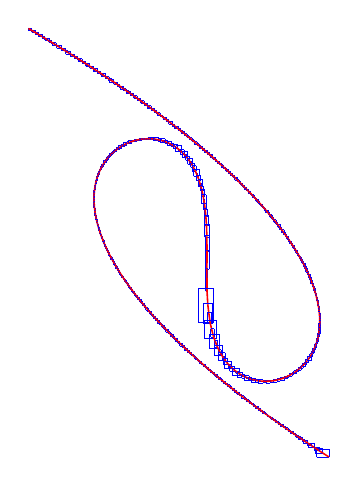
\begin{tikzpicture}[scale=4]
\draw[color=blue,line width=.1mm] (0.34823250691129837,-0.62562711397983) --(0.3874644072116633,-0.62562711397983);
\draw[color=blue,line width=.1mm] (0.34823250691129837,-0.62562711397983) --(0.34823250691129837,-0.6000265622358383);
\draw[color=blue,line width=.1mm] (0.34823250691129837,-0.6000265622358383) --(0.3874644072116633,-0.6000265622358383);
\draw[color=blue,line width=.1mm] (0.3874644072116633,-0.62562711397983) --(0.3874644072116633,-0.6000265622358383);
\draw[color=red,line width=.2mm] (0.3679054319594,-0.61275163442061) --(0.3871955483176678,-0.6252874189568768);
\draw[color=blue,line width=.1mm] (0.34368175157300296,-0.6128895028473611) --(0.36801446415205585,-0.6128895028473611);
\draw[color=blue,line width=.1mm] (0.34368175157300296,-0.6128895028473611) --(0.34368175157300296,-0.5969473391110345);
\draw[color=blue,line width=.1mm] (0.34368175157300296,-0.5969473391110345) --(0.36801446415205585,-0.5969473391110345);
\draw[color=blue,line width=.1mm] (0.36801446415205585,-0.6128895028473611) --(0.36801446415205585,-0.5969473391110345);
\draw[color=red,line width=.2mm] (0.35587149309736105,-0.6048878027318568) --(0.3679054319594,-0.61275163442061);
\draw[color=blue,line width=.1mm] (0.34078404925970035,-0.6049433002943974) --(0.35591524082849874,-0.6049433002943974);
\draw[color=blue,line width=.1mm] (0.34078404925970035,-0.6049433002943974) --(0.34078404925970035,-0.5950043475048719);
\draw[color=blue,line width=.1mm] (0.34078404925970035,-0.5950043475048719) --(0.35591524082849874,-0.5950043475048719);
\draw[color=blue,line width=.1mm] (0.35591524082849874,-0.6049433002943974) --(0.35591524082849874,-0.5950043475048719);
\draw[color=red,line width=.2mm] (0.34083326191154123,-0.5950528304901475) --(0.35587149309736105,-0.6048878027318568);
\draw[color=blue,line width=.1mm] (0.3216654663232162,-0.595652550099948) --(0.3411167651905685,-0.595652550099948);
\draw[color=blue,line width=.1mm] (0.3216654663232162,-0.595652550099948) --(0.3216654663232162,-0.5822714543658724);
\draw[color=blue,line width=.1mm] (0.3216654663232162,-0.5822714543658724) --(0.3411167651905685,-0.5822714543658724);
\draw[color=blue,line width=.1mm] (0.3411167651905685,-0.595652550099948) --(0.3411167651905685,-0.5822714543658724);
\draw[color=red,line width=.2mm] (0.331473517211649,-0.5888551402196763) --(0.34083326191154123,-0.5950528304901475);
\draw[color=blue,line width=.1mm] (0.31974142008736756,-0.5888962710241264) --(0.3315040276099092,-0.5888962710241264);
\draw[color=blue,line width=.1mm] (0.31974142008736756,-0.5888962710241264) --(0.31974142008736756,-0.5810694314941008);
\draw[color=blue,line width=.1mm] (0.31974142008736756,-0.5810694314941008) --(0.3315040276099092,-0.5810694314941008);
\draw[color=blue,line width=.1mm] (0.3315040276099092,-0.5888962710241264) --(0.3315040276099092,-0.5810694314941008);
\draw[color=red,line width=.2mm] (0.31977707653977216,-0.5811040057860473) --(0.331473517211649,-0.5888551402196763);
\draw[color=blue,line width=.1mm] (0.3049204552030939,-0.5814818856106818) --(0.31995788508588946,-0.5814818856106818);
\draw[color=blue,line width=.1mm] (0.3049204552030939,-0.5814818856106818) --(0.3049204552030939,-0.571107745601747);
\draw[color=blue,line width=.1mm] (0.3049204552030939,-0.571107745601747) --(0.31995788508588946,-0.571107745601747);
\draw[color=blue,line width=.1mm] (0.31995788508588946,-0.5814818856106818) --(0.31995788508588946,-0.571107745601747);
\draw[color=red,line width=.2mm] (0.3124917508072429,-0.5762276411193977) --(0.31977707653977216,-0.5811040057860473);
\draw[color=blue,line width=.1mm] (0.30336490984174486,-0.5762527813159894) --(0.312510794470851,-0.5762527813159894);
\draw[color=blue,line width=.1mm] (0.30336490984174486,-0.5762527813159894) --(0.30336490984174486,-0.5701085339271148);
\draw[color=blue,line width=.1mm] (0.30336490984174486,-0.5701085339271148) --(0.312510794470851,-0.5701085339271148);
\draw[color=blue,line width=.1mm] (0.312510794470851,-0.5762527813159894) --(0.312510794470851,-0.5701085339271148);
\draw[color=red,line width=.2mm] (0.30338705939886773,-0.5701297645238397) --(0.3124917508072429,-0.5762276411193977);
\draw[color=blue,line width=.1mm] (0.2918569490577359,-0.5703662854033025) --(0.3035013327900818,-0.5703662854033025);
\draw[color=blue,line width=.1mm] (0.2918569490577359,-0.5703662854033025) --(0.2918569490577359,-0.5623150118738847);
\draw[color=blue,line width=.1mm] (0.2918569490577359,-0.5623150118738847) --(0.3035013327900818,-0.5623150118738847);
\draw[color=blue,line width=.1mm] (0.3035013327900818,-0.5703662854033025) --(0.3035013327900818,-0.5623150118738847);
\draw[color=red,line width=.2mm] (0.29771238652083004,-0.5662986835390077) --(0.30338705939886773,-0.5701297645238397);
\draw[color=blue,line width=.1mm] (0.290606537679435,-0.5663140283885347) --(0.2977242121835507,-0.5663140283885347);
\draw[color=blue,line width=.1mm] (0.290606537679435,-0.5663140283885347) --(0.290606537679435,-0.5614953646453266);
\draw[color=blue,line width=.1mm] (0.290606537679435,-0.5614953646453266) --(0.2977242121835507,-0.5614953646453266);
\draw[color=blue,line width=.1mm] (0.2977242121835507,-0.5663140283885347) --(0.2977242121835507,-0.5614953646453266);
\draw[color=red,line width=.2mm] (0.290620236594689,-0.5615083737232223) --(0.29771238652083004,-0.5662986835390077);
\draw[color=blue,line width=.1mm] (0.281661377422199,-0.5616556440891007) --(0.290691940407771,-0.5616556440891007);
\draw[color=blue,line width=.1mm] (0.281661377422199,-0.5616556440891007) --(0.281661377422199,-0.5554006652837278);
\draw[color=blue,line width=.1mm] (0.281661377422199,-0.5554006652837278) --(0.290691940407771,-0.5554006652837278);
\draw[color=blue,line width=.1mm] (0.290691940407771,-0.5616556440891007) --(0.290691940407771,-0.5554006652837278);
\draw[color=red,line width=.2mm] (0.2861975267516452,-0.5585020654065207) --(0.290620236594689,-0.5615083737232223);
\draw[color=blue,line width=.1mm] (0.2806614162319989,-0.5585114245914876) --(0.28620484138006086,-0.5585114245914876);
\draw[color=blue,line width=.1mm] (0.2806614162319989,-0.5585114245914876) --(0.2806614162319989,-0.5547353397087856);
\draw[color=blue,line width=.1mm] (0.2806614162319989,-0.5547353397087856) --(0.28620484138006086,-0.5547353397087856);
\draw[color=blue,line width=.1mm] (0.28620484138006086,-0.5585114245914876) --(0.28620484138006086,-0.5547353397087856);
\draw[color=red,line width=.2mm] (0.28066986113925413,-0.5547432999056399) --(0.2861975267516452,-0.5585020654065207);
\draw[color=blue,line width=.1mm] (0.2737018298350928,-0.5548346148848912) --(0.28071459392163217,-0.5548346148848912);
\draw[color=blue,line width=.1mm] (0.2737018298350928,-0.5548346148848912) --(0.2737018298350928,-0.5499705387033434);
\draw[color=blue,line width=.1mm] (0.2737018298350928,-0.5499705387033434) --(0.28071459392163217,-0.5499705387033434);
\draw[color=blue,line width=.1mm] (0.28071459392163217,-0.5548346148848912) --(0.28071459392163217,-0.5499705387033434);
\draw[color=red,line width=.2mm] (0.2737692696303813,-0.5500336813268554) --(0.28066986113925413,-0.5547432999056399);
\draw[color=blue,line width=.1mm] (0.265050843812381,-0.5501778644184547) --(0.27384020843924495,-0.5501778644184547);
\draw[color=blue,line width=.1mm] (0.265050843812381,-0.5501778644184547) --(0.265050843812381,-0.5440292994108482);
\draw[color=blue,line width=.1mm] (0.265050843812381,-0.5440292994108482) --(0.27384020843924495,-0.5440292994108482);
\draw[color=blue,line width=.1mm] (0.27384020843924495,-0.5501778644184547) --(0.27384020843924495,-0.5440292994108482);
\draw[color=red,line width=.2mm] (0.2694661751532813,-0.5470780980347337) --(0.2737692696303813,-0.5500336813268554);
\draw[color=blue,line width=.1mm] (0.2640796845412875,-0.5470872404911075) --(0.2694733944486539,-0.5470872404911075);
\draw[color=blue,line width=.1mm] (0.2640796845412875,-0.5470872404911075) --(0.2640796845412875,-0.5433749819093078);
\draw[color=blue,line width=.1mm] (0.2640796845412875,-0.5433749819093078) --(0.2694733944486539,-0.5433749819093078);
\draw[color=blue,line width=.1mm] (0.2694733944486539,-0.5470872404911075) --(0.2694733944486539,-0.5433749819093078);
\draw[color=red,line width=.2mm] (0.2640880190701871,-0.5433827618479908) --(0.2694661751532813,-0.5470780980347337);
\draw[color=blue,line width=.1mm] (0.25730763017663766,-0.5434719334325311) --(0.2641321734178745,-0.5434719334325311);
\draw[color=blue,line width=.1mm] (0.25730763017663766,-0.5434719334325311) --(0.25730763017663766,-0.5386909949765797);
\draw[color=blue,line width=.1mm] (0.25730763017663766,-0.5386909949765797) --(0.2641321734178745,-0.5386909949765797);
\draw[color=blue,line width=.1mm] (0.2641321734178745,-0.5434719334325311) --(0.2641321734178745,-0.5386909949765797);
\draw[color=red,line width=.2mm] (0.2573741981636641,-0.538752716098539) --(0.2640880190701871,-0.5433827618479908);
\draw[color=blue,line width=.1mm] (0.24889044306922625,-0.538893500653315) --(0.2574442124213736,-0.538893500653315);
\draw[color=blue,line width=.1mm] (0.24889044306922625,-0.538893500653315) --(0.24889044306922625,-0.5328505087647802);
\draw[color=blue,line width=.1mm] (0.24889044306922625,-0.5328505087647802) --(0.2574442124213736,-0.5328505087647802);
\draw[color=blue,line width=.1mm] (0.2574442124213736,-0.538893500653315) --(0.2574442124213736,-0.5328505087647802);
\draw[color=red,line width=.2mm] (0.25318770781104066,-0.5358471767238028) --(0.2573741981636641,-0.538752716098539);
\draw[color=blue,line width=.1mm] (0.24794707482133915,-0.5358561033878904) --(0.2531948303868451,-0.5358561033878904);
\draw[color=blue,line width=.1mm] (0.24794707482133915,-0.5358561033878904) --(0.24794707482133915,-0.5322068176371648);
\draw[color=blue,line width=.1mm] (0.24794707482133915,-0.5322068176371648) --(0.2531948303868451,-0.5322068176371648);
\draw[color=blue,line width=.1mm] (0.2531948303868451,-0.5358561033878904) --(0.2531948303868451,-0.5322068176371648);
\draw[color=red,line width=.2mm] (0.24795529694761936,-0.5322144183510927) --(0.25318770781104066,-0.5358471767238028);
\draw[color=blue,line width=.1mm] (0.24135784913538375,-0.5323014765026381) --(0.24799886975539268,-0.5323014765026381);
\draw[color=blue,line width=.1mm] (0.24135784913538375,-0.5323014765026381) --(0.24135784913538375,-0.5276025583307127);
\draw[color=blue,line width=.1mm] (0.24135784913538375,-0.5276025583307127) --(0.24799886975539268,-0.5276025583307127);
\draw[color=blue,line width=.1mm] (0.24799886975539268,-0.5323014765026381) --(0.24799886975539268,-0.5276025583307127);
\draw[color=red,line width=.2mm] (0.2414235406352793,-0.5276628765461169) --(0.24795529694761936,-0.5322144183510927);
\draw[color=blue,line width=.1mm] (0.23316858006513005,-0.5278003103845181) --(0.2414926255202133,-0.5278003103845181);
\draw[color=blue,line width=.1mm] (0.23316858006513005,-0.5278003103845181) --(0.23316858006513005,-0.5218614707951561);
\draw[color=blue,line width=.1mm] (0.23316858006513005,-0.5218614707951561) --(0.2414926255202133,-0.5218614707951561);
\draw[color=blue,line width=.1mm] (0.2414926255202133,-0.5278003103845181) --(0.2414926255202133,-0.5218614707951561);
\draw[color=red,line width=.2mm] (0.237350712487047,-0.5248067081042866) --(0.2414235406352793,-0.5276628765461169);
\draw[color=blue,line width=.1mm] (0.23225226020447,-0.5248154219863117) --(0.23735773788218642,-0.5248154219863117);
\draw[color=blue,line width=.1mm] (0.23225226020447,-0.5248154219863117) --(0.23225226020447,-0.5212282620433306);
\draw[color=blue,line width=.1mm] (0.23225226020447,-0.5212282620433306) --(0.23735773788218642,-0.5212282620433306);
\draw[color=blue,line width=.1mm] (0.23735773788218642,-0.5248154219863117) --(0.23735773788218642,-0.5212282620433306);
\draw[color=red,line width=.2mm] (0.2322603694008156,-0.5212356859333279) --(0.237350712487047,-0.5248067081042866);
\draw[color=blue,line width=.1mm] (0.22584126973004373,-0.5213206606156906) --(0.23230335771575397,-0.5213206606156906);
\draw[color=blue,line width=.1mm] (0.22584126973004373,-0.5213206606156906) --(0.22584126973004373,-0.5167026576335207);
\draw[color=blue,line width=.1mm] (0.22584126973004373,-0.5167026576335207) --(0.23230335771575397,-0.5167026576335207);
\draw[color=blue,line width=.1mm] (0.23230335771575397,-0.5213206606156906) --(0.23230335771575397,-0.5167026576335207);
\draw[color=red,line width=.2mm] (0.2259060802862123,-0.5167615915532471) --(0.2322603694008156,-0.5212356859333279);
\draw[color=blue,line width=.1mm] (0.217874173563529,-0.5168957224528506) --(0.22597423115183712,-0.5168957224528506);
\draw[color=blue,line width=.1mm] (0.217874173563529,-0.5168957224528506) --(0.217874173563529,-0.5110596298696558);
\draw[color=blue,line width=.1mm] (0.217874173563529,-0.5110596298696558) --(0.22597423115183712,-0.5110596298696558);
\draw[color=blue,line width=.1mm] (0.22597423115183712,-0.5168957224528506) --(0.22597423115183712,-0.5110596298696558);
\draw[color=red,line width=.2mm] (0.22194404033506399,-0.5139541287950813) --(0.2259060802862123,-0.5167615915532471);
\draw[color=blue,line width=.1mm] (0.21698417672241185,-0.5139626329176097) --(0.22195096809964007,-0.5139626329176097);
\draw[color=blue,line width=.1mm] (0.21698417672241185,-0.5139626329176097) --(0.21698417672241185,-0.5104367614033252);
\draw[color=blue,line width=.1mm] (0.21698417672241185,-0.5104367614033252) --(0.22195096809964007,-0.5104367614033252);
\draw[color=blue,line width=.1mm] (0.22195096809964007,-0.5139626329176097) --(0.22195096809964007,-0.5104367614033252);
\draw[color=red,line width=.2mm] (0.21699217247740832,-0.5104440108830505) --(0.22194404033506399,-0.5139541287950813);
\draw[color=blue,line width=.1mm] (0.21074693395578964,-0.5105269320378617) --(0.21703457347260285,-0.5105269320378617);
\draw[color=blue,line width=.1mm] (0.21074693395578964,-0.5105269320378617) --(0.21074693395578964,-0.5059887512729225);
\draw[color=blue,line width=.1mm] (0.21074693395578964,-0.5059887512729225) --(0.21703457347260285,-0.5059887512729225);
\draw[color=blue,line width=.1mm] (0.21703457347260285,-0.5105269320378617) --(0.21703457347260285,-0.5059887512729225);
\draw[color=red,line width=.2mm] (0.21081085931035518,-0.5060463195012797) --(0.21699217247740832,-0.5104440108830505);
\draw[color=blue,line width=.1mm] (0.20299639808590095,-0.5061771952561108) --(0.21087807179364412,-0.5061771952561108);
\draw[color=blue,line width=.1mm] (0.20299639808590095,-0.5061771952561108) --(0.20299639808590095,-0.5004424594545859);
\draw[color=blue,line width=.1mm] (0.20299639808590095,-0.5004424594545859) --(0.21087807179364412,-0.5004424594545859);
\draw[color=blue,line width=.1mm] (0.21087807179364412,-0.5061771952561108) --(0.21087807179364412,-0.5004424594545859);
\draw[color=red,line width=.2mm] (0.2069567999229257,-0.5032869047423361) --(0.21081085931035518,-0.5060463195012797);
\draw[color=blue,line width=.1mm] (0.20213228398031968,-0.5032950805625097) --(0.2069659640995105,-0.5032950805625097);
\draw[color=blue,line width=.1mm] (0.20213228398031968,-0.5032950805625097) --(0.20213228398031968,-0.4998268736534902);
\draw[color=blue,line width=.1mm] (0.20213228398031968,-0.4998268736534902) --(0.2069659640995105,-0.4998268736534902);
\draw[color=blue,line width=.1mm] (0.2069659640995105,-0.5032950805625097) --(0.2069659640995105,-0.4998268736534902);
\draw[color=red,line width=.2mm] (0.202137909029456,-0.49983919080060935) --(0.2069567999229257,-0.5032869047423361);
\draw[color=blue,line width=.1mm] (0.1960299686335802,-0.49996356650517176) --(0.20220268483643483,-0.49996356650517176);
\draw[color=blue,line width=.1mm] (0.1960299686335802,-0.49996356650517176) --(0.1960299686335802,-0.49542788894613826);
\draw[color=blue,line width=.1mm] (0.1960299686335802,-0.49542788894613826) --(0.20220268483643483,-0.49542788894613826);
\draw[color=blue,line width=.1mm] (0.20220268483643483,-0.49996356650517176) --(0.20220268483643483,-0.49542788894613826);
\draw[color=red,line width=.2mm] (0.19913509395833515,-0.49767390478262274) --(0.202137909029456,-0.49983919080060935);
\draw[color=blue,line width=.1mm] (0.19536422718361046,-0.4976942340854367) --(0.19915796513291917,-0.4976942340854367);
\draw[color=blue,line width=.1mm] (0.19536422718361046,-0.4976942340854367) --(0.19536422718361046,-0.4949405715942777);
\draw[color=blue,line width=.1mm] (0.19536422718361046,-0.4949405715942777) --(0.19915796513291917,-0.4949405715942777);
\draw[color=blue,line width=.1mm] (0.19915796513291917,-0.4976942340854367) --(0.19915796513291917,-0.4949405715942777);
\draw[color=red,line width=.2mm] (0.1953782630357211,-0.4949711551681721) --(0.19913509395833515,-0.49767390478262274);
\draw[color=blue,line width=.1mm] (0.19062983948089327,-0.4950480348426377) --(0.19541849964872612,-0.4950480348426377);
\draw[color=blue,line width=.1mm] (0.19062983948089327,-0.4950480348426377) --(0.19062983948089327,-0.49152986964430834);
\draw[color=blue,line width=.1mm] (0.19062983948089327,-0.49152986964430834) --(0.19541849964872612,-0.49152986964430834);
\draw[color=blue,line width=.1mm] (0.19541849964872612,-0.4950480348426377) --(0.19541849964872612,-0.49152986964430834);
\draw[color=red,line width=.2mm] (0.1906902182068706,-0.4915834710528024) --(0.1953782630357211,-0.4949711551681721);
\draw[color=blue,line width=.1mm] (0.18478566696465476,-0.4916480230612121) --(0.1907247035505692,-0.4916480230612121);
\draw[color=blue,line width=.1mm] (0.18478566696465476,-0.4916480230612121) --(0.18478566696465476,-0.48729583038301433);
\draw[color=blue,line width=.1mm] (0.18478566696465476,-0.48729583038301433) --(0.1907247035505692,-0.48729583038301433);
\draw[color=blue,line width=.1mm] (0.1907247035505692,-0.4916480230612121) --(0.1907247035505692,-0.48729583038301433);
\draw[color=red,line width=.2mm] (0.18483686418073675,-0.48734115614821044) --(0.1906902182068706,-0.4915834710528024);
\draw[color=blue,line width=.1mm] (0.17743544925411012,-0.48746502172034295) --(0.18490170705859096,-0.48746502172034295);
\draw[color=blue,line width=.1mm] (0.17743544925411012,-0.48746502172034295) --(0.17743544925411012,-0.4819371372828732);
\draw[color=blue,line width=.1mm] (0.17743544925411012,-0.4819371372828732) --(0.18490170705859096,-0.4819371372828732);
\draw[color=blue,line width=.1mm] (0.18490170705859096,-0.48746502172034295) --(0.18490170705859096,-0.4819371372828732);
\draw[color=red,line width=.2mm] (0.18118745307322529,-0.48467947600138755) --(0.18483686418073675,-0.48734115614821044);
\draw[color=blue,line width=.1mm] (0.17661898560277414,-0.48468723606015757) --(0.18119630252135913,-0.48468723606015757);
\draw[color=blue,line width=.1mm] (0.17661898560277414,-0.48468723606015757) --(0.17661898560277414,-0.4813421756505288);
\draw[color=blue,line width=.1mm] (0.17661898560277414,-0.4813421756505288) --(0.18119630252135913,-0.4813421756505288);
\draw[color=blue,line width=.1mm] (0.18119630252135913,-0.48468723606015757) --(0.18119630252135913,-0.4813421756505288);
\draw[color=red,line width=.2mm] (0.17662441743973617,-0.48135384262337266) --(0.18118745307322529,-0.48467947600138755);
\draw[color=blue,line width=.1mm] (0.17083926186145137,-0.48147157912371935) --(0.17668691434786044,-0.48147157912371935);
\draw[color=blue,line width=.1mm] (0.17083926186145137,-0.48147157912371935) --(0.17083926186145137,-0.4771004769883819);
\draw[color=blue,line width=.1mm] (0.17083926186145137,-0.4771004769883819) --(0.17668691434786044,-0.4771004769883819);
\draw[color=blue,line width=.1mm] (0.17668691434786044,-0.48147157912371935) --(0.17668691434786044,-0.4771004769883819);
\draw[color=red,line width=.2mm] (0.17093304138416632,-0.47718267721672925) --(0.17662441743973617,-0.48135384262337266);
\draw[color=blue,line width=.1mm] (0.16374935530199455,-0.47728197637996117) --(0.17098688651036956,-0.47728197637996117);
\draw[color=blue,line width=.1mm] (0.16374935530199455,-0.47728197637996117) --(0.16374935530199455,-0.4718870655248588);
\draw[color=blue,line width=.1mm] (0.16374935530199455,-0.4718870655248588) --(0.17098688651036956,-0.4718870655248588);
\draw[color=blue,line width=.1mm] (0.17098688651036956,-0.47728197637996117) --(0.17098688651036956,-0.4718870655248588);
\draw[color=red,line width=.2mm] (0.16382929426011106,-0.47195689268571267) --(0.17093304138416632,-0.47718267721672925);
\draw[color=blue,line width=.1mm] (0.15481716088539202,-0.47214744041211637) --(0.1639306853146593,-0.47214744041211637);
\draw[color=blue,line width=.1mm] (0.15481716088539202,-0.47214744041211637) --(0.15481716088539202,-0.46526894102662303);
\draw[color=blue,line width=.1mm] (0.15481716088539202,-0.46526894102662303) --(0.1639306853146593,-0.46526894102662303);
\draw[color=blue,line width=.1mm] (0.1639306853146593,-0.47214744041211637) --(0.1639306853146593,-0.46526894102662303);
\draw[color=red,line width=.2mm] (0.1594034287956442,-0.468675081113332) --(0.16382929426011106,-0.47195689268571267);
\draw[color=blue,line width=.1mm] (0.15386007375591962,-0.4686873973657582) --(0.15941385582946768,-0.4686873973657582);
\draw[color=blue,line width=.1mm] (0.15386007375591962,-0.4686873973657582) --(0.15386007375591962,-0.46456118156831666);
\draw[color=blue,line width=.1mm] (0.15386007375591962,-0.46456118156831666) --(0.15941385582946768,-0.46456118156831666);
\draw[color=blue,line width=.1mm] (0.15941385582946768,-0.4686873973657582) --(0.15941385582946768,-0.46456118156831666);
\draw[color=red,line width=.2mm] (0.1538721408505909,-0.464571681461802) --(0.1594034287956442,-0.468675081113332);
\draw[color=blue,line width=.1mm] (0.14687522801264266,-0.4646898540934024) --(0.15393552082982923,-0.4646898540934024);
\draw[color=blue,line width=.1mm] (0.14687522801264266,-0.4646898540934024) --(0.14687522801264266,-0.45934583046367045);
\draw[color=blue,line width=.1mm] (0.14687522801264266,-0.45934583046367045) --(0.15393552082982923,-0.45934583046367045);
\draw[color=blue,line width=.1mm] (0.15393552082982923,-0.4646898540934024) --(0.15393552082982923,-0.45934583046367045);
\draw[color=red,line width=.2mm] (0.1504238213392097,-0.46199734333354564) --(0.1538721408505909,-0.464571681461802);
\draw[color=blue,line width=.1mm] (0.1461068563163003,-0.4620047804694721) --(0.15043248843864557,-0.4620047804694721);
\draw[color=blue,line width=.1mm] (0.1461068563163003,-0.4620047804694721) --(0.1461068563163003,-0.45876966351559784);
\draw[color=blue,line width=.1mm] (0.1461068563163003,-0.45876966351559784) --(0.15043248843864557,-0.45876966351559784);
\draw[color=blue,line width=.1mm] (0.15043248843864557,-0.4620047804694721) --(0.15043248843864557,-0.45876966351559784);
\draw[color=red,line width=.2mm] (0.14611217620912662,-0.45878081577696345) --(0.1504238213392097,-0.46199734333354564);
\draw[color=blue,line width=.1mm] (0.1406429861308695,-0.45889331613289125) --(0.14617334577636004,-0.45889331613289125);
\draw[color=blue,line width=.1mm] (0.1406429861308695,-0.45889331613289125) --(0.1406429861308695,-0.45466800281865455);
\draw[color=blue,line width=.1mm] (0.1406429861308695,-0.45466800281865455) --(0.14617334577636004,-0.45466800281865455);
\draw[color=blue,line width=.1mm] (0.14617334577636004,-0.45889331613289125) --(0.14617334577636004,-0.45466800281865455);
\draw[color=red,line width=.2mm] (0.1407347745330107,-0.45474673584805503) --(0.14611217620912662,-0.45878081577696345);
\draw[color=blue,line width=.1mm] (0.1339450463766142,-0.4548415997995174) --(0.14078746412095178,-0.4548415997995174);
\draw[color=blue,line width=.1mm] (0.1339450463766142,-0.4548415997995174) --(0.1339450463766142,-0.44962603365984916);
\draw[color=blue,line width=.1mm] (0.1339450463766142,-0.44962603365984916) --(0.14078746412095178,-0.44962603365984916);
\draw[color=blue,line width=.1mm] (0.14078746412095178,-0.4548415997995174) --(0.14078746412095178,-0.44962603365984916);
\draw[color=red,line width=.2mm] (0.13402327022179567,-0.4496929008412827) --(0.1407347745330107,-0.45474673584805503);
\draw[color=blue,line width=.1mm] (0.12550430053821227,-0.44987489884927134) --(0.13412247055535598,-0.44987489884927134);
\draw[color=blue,line width=.1mm] (0.12550430053821227,-0.44987489884927134) --(0.12550430053821227,-0.44322668674551613);
\draw[color=blue,line width=.1mm] (0.12550430053821227,-0.44322668674551613) --(0.13412247055535598,-0.44322668674551613);
\draw[color=blue,line width=.1mm] (0.13412247055535598,-0.44987489884927134) --(0.13412247055535598,-0.44322668674551613);
\draw[color=red,line width=.2mm] (0.12984225421774268,-0.4465193469466683) --(0.13402327022179567,-0.4496929008412827);
\draw[color=blue,line width=.1mm] (0.12460520895754174,-0.4465311114549293) --(0.12985244772633026,-0.4465311114549293);
\draw[color=blue,line width=.1mm] (0.12460520895754174,-0.4465311114549293) --(0.12460520895754174,-0.4425412852364714);
\draw[color=blue,line width=.1mm] (0.12460520895754174,-0.4425412852364714) --(0.12985244772633026,-0.4425412852364714);
\draw[color=blue,line width=.1mm] (0.12985244772633026,-0.4465311114549293) --(0.12985244772633026,-0.4425412852364714);
\draw[color=red,line width=.2mm] (0.12461700349703705,-0.442551329053759) --(0.12984225421774268,-0.4465193469466683);
\draw[color=blue,line width=.1mm] (0.11800445080989362,-0.44266416195859193) --(0.12467899456787478,-0.44266416195859193);
\draw[color=blue,line width=.1mm] (0.11800445080989362,-0.44266416195859193) --(0.11800445080989362,-0.43749895323816446);
\draw[color=blue,line width=.1mm] (0.11800445080989362,-0.43749895323816446) --(0.12467899456787478,-0.43749895323816446);
\draw[color=blue,line width=.1mm] (0.12467899456787478,-0.44266416195859193) --(0.12467899456787478,-0.43749895323816446);
\draw[color=red,line width=.2mm] (0.11809790102832758,-0.4375778555803914) --(0.12461700349703705,-0.442551329053759);
\draw[color=blue,line width=.1mm] (0.10982027564099571,-0.43775625709485494) --(0.11819645285217138,-0.43775625709485494);
\draw[color=blue,line width=.1mm] (0.10982027564099571,-0.43775625709485494) --(0.10982027564099571,-0.4312149338215869);
\draw[color=blue,line width=.1mm] (0.10982027564099571,-0.4312149338215869) --(0.11819645285217138,-0.4312149338215869);
\draw[color=blue,line width=.1mm] (0.11819645285217138,-0.43775625709485494) --(0.11819645285217138,-0.4312149338215869);
\draw[color=red,line width=.2mm] (0.114037045615732,-0.4344548718951289) --(0.11809790102832758,-0.4375778555803914);
\draw[color=blue,line width=.1mm] (0.10895028023508672,-0.43446640109845963) --(0.11404716451937162,-0.43446640109845963);
\draw[color=blue,line width=.1mm] (0.10895028023508672,-0.43446640109845963) --(0.10895028023508672,-0.4305402425941319);
\draw[color=blue,line width=.1mm] (0.10895028023508672,-0.4305402425941319) --(0.11404716451937162,-0.4305402425941319);
\draw[color=blue,line width=.1mm] (0.11404716451937162,-0.43446640109845963) --(0.11404716451937162,-0.4305402425941319);
\draw[color=red,line width=.2mm] (0.10896198777473738,-0.43055009308485587) --(0.114037045615732,-0.4344548718951289);
\draw[color=blue,line width=.1mm] (0.10253775687875265,-0.4306606144432404) --(0.10902353411643805,-0.4306606144432404);
\draw[color=blue,line width=.1mm] (0.10253775687875265,-0.4306606144432404) --(0.10253775687875265,-0.42557859211001375);
\draw[color=blue,line width=.1mm] (0.10253775687875265,-0.42557859211001375) --(0.10902353411643805,-0.42557859211001375);
\draw[color=blue,line width=.1mm] (0.10902353411643805,-0.4306606144432404) --(0.10902353411643805,-0.42557859211001375);
\draw[color=red,line width=.2mm] (0.10263053695425053,-0.4256559875415982) --(0.10896198777473738,-0.43055009308485587);
\draw[color=blue,line width=.1mm] (0.09458841019099631,-0.425830715150786) --(0.10272837335091603,-0.425830715150786);
\draw[color=blue,line width=.1mm] (0.09458841019099631,-0.425830715150786) --(0.09458841019099631,-0.4193951788078802);
\draw[color=blue,line width=.1mm] (0.09458841019099631,-0.4193951788078802) --(0.10272837335091603,-0.4193951788078802);
\draw[color=blue,line width=.1mm] (0.10272837335091603,-0.425830715150786) --(0.10272837335091603,-0.4193951788078802);
\draw[color=red,line width=.2mm] (0.09868686510484752,-0.4225829563090164) --(0.10263053695425053,-0.4256559875415982);
\draw[color=blue,line width=.1mm] (0.0937466604776703,-0.42259425133501155) --(0.09869690748416113,-0.42259425133501155);
\draw[color=blue,line width=.1mm] (0.0937466604776703,-0.42259425133501155) --(0.0937466604776703,-0.41873098609916143);
\draw[color=blue,line width=.1mm] (0.0937466604776703,-0.41873098609916143) --(0.09869690748416113,-0.41873098609916143);
\draw[color=blue,line width=.1mm] (0.09869690748416113,-0.42259425133501155) --(0.09869690748416113,-0.41873098609916143);
\draw[color=red,line width=.2mm] (0.09375827860847281,-0.41874064420596635) --(0.09868686510484752,-0.4225829563090164);
\draw[color=blue,line width=.1mm] (0.08751772971768365,-0.4188488734406726) --(0.09381937093453449,-0.4188488734406726);
\draw[color=blue,line width=.1mm] (0.08751772971768365,-0.4188488734406726) --(0.08751772971768365,-0.4138490380400051);
\draw[color=blue,line width=.1mm] (0.08751772971768365,-0.4138490380400051) --(0.09381937093453449,-0.4138490380400051);
\draw[color=blue,line width=.1mm] (0.09381937093453449,-0.4188488734406726) --(0.09381937093453449,-0.4138490380400051);
\draw[color=red,line width=.2mm] (0.08760982564686322,-0.41392493792926793) --(0.09375827860847281,-0.41874064420596635);
\draw[color=blue,line width=.1mm] (0.07979739982045995,-0.4140960226199688) --(0.08770693164195674,-0.4140960226199688);
\draw[color=blue,line width=.1mm] (0.07979739982045995,-0.4140960226199688) --(0.07979739982045995,-0.40776500816577865);
\draw[color=blue,line width=.1mm] (0.07979739982045995,-0.40776500816577865) --(0.08770693164195674,-0.40776500816577865);
\draw[color=blue,line width=.1mm] (0.08770693164195674,-0.4140960226199688) --(0.08770693164195674,-0.40776500816577865);
\draw[color=red,line width=.2mm] (0.08378042668010874,-0.4109012502342875) --(0.08760982564686322,-0.41392493792926793);
\draw[color=blue,line width=.1mm] (0.0789831461547225,-0.41091231295273767) --(0.08379039093729139,-0.41091231295273767);
\draw[color=blue,line width=.1mm] (0.0789831461547225,-0.41091231295273767) --(0.0789831461547225,-0.40711117626039206);
\draw[color=blue,line width=.1mm] (0.0789831461547225,-0.40711117626039206) --(0.08379039093729139,-0.40711117626039206);
\draw[color=blue,line width=.1mm] (0.08379039093729139,-0.41091231295273767) --(0.08379039093729139,-0.40711117626039206);
\draw[color=red,line width=.2mm] (0.07899467300926359,-0.40712064342155935) --(0.08378042668010874,-0.4109012502342875);
\draw[color=blue,line width=.1mm] (0.07293327038332395,-0.40722659997175525) --(0.07905530181432882,-0.40722659997175525);
\draw[color=blue,line width=.1mm] (0.07293327038332395,-0.40722659997175525) --(0.07293327038332395,-0.40230796573508143);
\draw[color=blue,line width=.1mm] (0.07293327038332395,-0.40230796573508143) --(0.07905530181432882,-0.40230796573508143);
\draw[color=blue,line width=.1mm] (0.07905530181432882,-0.40722659997175525) --(0.07905530181432882,-0.40230796573508143);
\draw[color=red,line width=.2mm] (0.07302466785011621,-0.40238238143220073) --(0.07899467300926359,-0.40712064342155935);
\draw[color=blue,line width=.1mm] (0.06543627528538896,-0.402549854263424) --(0.07312102821255072,-0.402549854263424);
\draw[color=blue,line width=.1mm] (0.06543627528538896,-0.402549854263424) --(0.06543627528538896,-0.39632211365293996);
\draw[color=blue,line width=.1mm] (0.06543627528538896,-0.39632211365293996) --(0.07312102821255072,-0.39632211365293996);
\draw[color=blue,line width=.1mm] (0.07312102821255072,-0.402549854263424) --(0.07312102821255072,-0.39632211365293996);
\draw[color=red,line width=.2mm] (0.06930669587868045,-0.399407436896111) --(0.07302466785011621,-0.40238238143220073);
\draw[color=blue,line width=.1mm] (0.0646487838232194,-0.39941826918139417) --(0.06931658038884661,-0.39941826918139417);
\draw[color=blue,line width=.1mm] (0.0646487838232194,-0.39941826918139417) --(0.0646487838232194,-0.39567850697049584);
\draw[color=blue,line width=.1mm] (0.0646487838232194,-0.39567850697049584) --(0.06931658038884661,-0.39567850697049584);
\draw[color=blue,line width=.1mm] (0.06931658038884661,-0.39941826918139417) --(0.06931658038884661,-0.39567850697049584);
\draw[color=red,line width=.2mm] (0.064660217503434,-0.39568778462497506) --(0.06930669587868045,-0.399407436896111);
\draw[color=blue,line width=.1mm] (0.058773526840624805,-0.3957914879927442) --(0.0647203731338521,-0.3957914879927442);
\draw[color=blue,line width=.1mm] (0.058773526840624805,-0.3957914879927442) --(0.058773526840624805,-0.39095308238646553);
\draw[color=blue,line width=.1mm] (0.058773526840624805,-0.39095308238646553) --(0.0647203731338521,-0.39095308238646553);
\draw[color=blue,line width=.1mm] (0.0647203731338521,-0.3957914879927442) --(0.0647203731338521,-0.39095308238646553);
\draw[color=red,line width=.2mm] (0.058864211291653465,-0.3910260252619158) --(0.064660217503434,-0.39568778462497506);
\draw[color=blue,line width=.1mm] (0.051494311176012546,-0.39118991736595715) --(0.05895981051284382,-0.39118991736595715);
\draw[color=blue,line width=.1mm] (0.051494311176012546,-0.39118991736595715) --(0.051494311176012546,-0.3850642190996973);
\draw[color=blue,line width=.1mm] (0.051494311176012546,-0.3850642190996973) --(0.05895981051284382,-0.3850642190996973);
\draw[color=blue,line width=.1mm] (0.05895981051284382,-0.39118991736595715) --(0.05895981051284382,-0.3850642190996973);
\draw[color=red,line width=.2mm] (0.055254883641779586,-0.38809923180959843) --(0.058864211291653465,-0.3910260252619158);
\draw[color=blue,line width=.1mm] (0.05073286346002169,-0.3881098355535394) --(0.05526468676240802,-0.3881098355535394);
\draw[color=blue,line width=.1mm] (0.05073286346002169,-0.3881098355535394) --(0.05073286346002169,-0.3844307041084428);
\draw[color=blue,line width=.1mm] (0.05073286346002169,-0.3844307041084428) --(0.05526468676240802,-0.3844307041084428);
\draw[color=blue,line width=.1mm] (0.05526468676240802,-0.3881098355535394) --(0.05526468676240802,-0.3844307041084428);
\draw[color=red,line width=.2mm] (0.050744202047074256,-0.38443979370823006) --(0.055254883641779586,-0.38809923180959843);
\draw[color=blue,line width=.1mm] (0.045027888029745576,-0.38454126346114054) --(0.05080387468378924,-0.38454126346114054);
\draw[color=blue,line width=.1mm] (0.045027888029745576,-0.38454126346114054) --(0.045027888029745576,-0.37978212682282747);
\draw[color=blue,line width=.1mm] (0.045027888029745576,-0.37978212682282747) --(0.05080387468378924,-0.37978212682282747);
\draw[color=blue,line width=.1mm] (0.05080387468378924,-0.38454126346114054) --(0.05080387468378924,-0.37978212682282747);
\draw[color=red,line width=.2mm] (0.04511784466354749,-0.3798536082609609) --(0.050744202047074256,-0.38443979370823006);
\draw[color=blue,line width=.1mm] (0.03796101994230813,-0.38001395093441864) --(0.04521266697411594,-0.38001395093441864);
\draw[color=blue,line width=.1mm] (0.03796101994230813,-0.38001395093441864) --(0.03796101994230813,-0.3739890794254203);
\draw[color=blue,line width=.1mm] (0.03796101994230813,-0.3739890794254203) --(0.04521266697411594,-0.3739890794254203);
\draw[color=blue,line width=.1mm] (0.04521266697411594,-0.38001395093441864) --(0.04521266697411594,-0.3739890794254203);
\draw[color=red,line width=.2mm] (0.04161444033707641,-0.3769743818872374) --(0.04511784466354749,-0.3798536082609609);
\draw[color=blue,line width=.1mm] (0.03722491256124287,-0.3769847589804945) --(0.041624160392558604,-0.3769847589804945);
\draw[color=blue,line width=.1mm] (0.03722491256124287,-0.3769847589804945) --(0.03722491256124287,-0.3733655246773074);
\draw[color=blue,line width=.1mm] (0.03722491256124287,-0.3733655246773074) --(0.041624160392558604,-0.3733655246773074);
\draw[color=blue,line width=.1mm] (0.041624160392558604,-0.3769847589804945) --(0.041624160392558604,-0.3733655246773074);
\draw[color=red,line width=.2mm] (0.03723615410054394,-0.37337442766836504) --(0.04161444033707641,-0.3769743818872374);
\draw[color=blue,line width=.1mm] (0.03168597797294957,-0.37347368348496734) --(0.03729533377437498,-0.37347368348496734);
\draw[color=blue,line width=.1mm] (0.03168597797294957,-0.37347368348496734) --(0.03168597797294957,-0.36879286857225);
\draw[color=blue,line width=.1mm] (0.03168597797294957,-0.36879286857225) --(0.03729533377437498,-0.36879286857225);
\draw[color=blue,line width=.1mm] (0.03729533377437498,-0.37347368348496734) --(0.03729533377437498,-0.36879286857225);
\draw[color=red,line width=.2mm] (0.03177519176215598,-0.3688629000079652) --(0.03723615410054394,-0.37337442766836504);
\draw[color=blue,line width=.1mm] (0.024826146096256652,-0.36901972470727673) --(0.03186922116738054,-0.36901972470727673);
\draw[color=blue,line width=.1mm] (0.024826146096256652,-0.36901972470727673) --(0.024826146096256652,-0.3630944798372632);
\draw[color=blue,line width=.1mm] (0.024826146096256652,-0.3630944798372632) --(0.03186922116738054,-0.3630944798372632);
\draw[color=blue,line width=.1mm] (0.03186922116738054,-0.36901972470727673) --(0.03186922116738054,-0.3630944798372632);
\draw[color=red,line width=.2mm] (0.028375049939644546,-0.36603066454321315) --(0.03177519176215598,-0.3688629000079652);
\draw[color=blue,line width=.1mm] (0.024114690337962905,-0.3660408169016782) --(0.028384685242424688,-0.3660408169016782);
\draw[color=blue,line width=.1mm] (0.024114690337962905,-0.3660408169016782) --(0.024114690337962905,-0.3624807558626535);
\draw[color=blue,line width=.1mm] (0.024114690337962905,-0.3624807558626535) --(0.028384685242424688,-0.3624807558626535);
\draw[color=blue,line width=.1mm] (0.028384685242424688,-0.3660408169016782) --(0.028384685242424688,-0.3624807558626535);
\draw[color=red,line width=.2mm] (0.02412583286080839,-0.3624894737108603) --(0.028375049939644546,-0.36603066454321315);
\draw[color=blue,line width=.1mm] (0.018737650075263235,-0.3625865353928185) --(0.02418450946329337,-0.3625865353928185);
\draw[color=blue,line width=.1mm] (0.018737650075263235,-0.3625865353928185) --(0.018737650075263235,-0.3579831069977609);
\draw[color=blue,line width=.1mm] (0.018737650075263235,-0.3579831069977609) --(0.02418450946329337,-0.3579831069977609);
\draw[color=blue,line width=.1mm] (0.02418450946329337,-0.3625865353928185) --(0.02418450946329337,-0.3579831069977609);
\draw[color=red,line width=.2mm] (0.018826105784919004,-0.35805169992000285) --(0.02412583286080839,-0.3624894737108603);
\draw[color=blue,line width=.1mm] (0.012079660585030051,-0.3582050383326184) --(0.01891932610381262,-0.3582050383326184);
\draw[color=blue,line width=.1mm] (0.012079660585030051,-0.3582050383326184) --(0.012079660585030051,-0.35237823485537023);
\draw[color=blue,line width=.1mm] (0.012079660585030051,-0.35237823485537023) --(0.01891932610381262,-0.35237823485537023);
\draw[color=blue,line width=.1mm] (0.01891932610381262,-0.3582050383326184) --(0.01891932610381262,-0.35237823485537023);
\draw[color=red,line width=.2mm] (0.015526624369296102,-0.3552658867952069) --(0.018826105784919004,-0.35805169992000285);
\draw[color=blue,line width=.1mm] (0.011392182137101517,-0.35527581635512634) --(0.015536173208133877,-0.35527581635512634);
\draw[color=blue,line width=.1mm] (0.011392182137101517,-0.35527581635512634) --(0.011392182137101517,-0.3517742141648998);
\draw[color=blue,line width=.1mm] (0.011392182137101517,-0.3517742141648998) --(0.015536173208133877,-0.3517742141648998);
\draw[color=blue,line width=.1mm] (0.015536173208133877,-0.35527581635512634) --(0.015536173208133877,-0.3517742141648998);
\draw[color=red,line width=.2mm] (0.011403223649465711,-0.3517827483507409) --(0.015526624369296102,-0.3552658867952069);
\draw[color=blue,line width=.1mm] (0.006172981562200848,-0.35187763585992404) --(0.011461386957022741,-0.35187763585992404);
\draw[color=blue,line width=.1mm] (0.006172981562200848,-0.35187763585992404) --(0.006172981562200848,-0.3473506703724667);
\draw[color=blue,line width=.1mm] (0.006172981562200848,-0.3473506703724667) --(0.011461386957022741,-0.3473506703724667);
\draw[color=blue,line width=.1mm] (0.011461386957022741,-0.35187763585992404) --(0.011461386957022741,-0.3473506703724667);
\draw[color=red,line width=.2mm] (0.006260663781979988,-0.34741783635292484) --(0.011403223649465711,-0.3517827483507409);
\draw[color=blue,line width=.1mm] (-0.0002882446269707249,-0.3475677204569619) --(0.006353058634887686,-0.3475677204569619);
\draw[color=blue,line width=.1mm] (-0.0002882446269707249,-0.3475677204569619) --(-0.0002882446269707249,-0.3418381874235164);
\draw[color=blue,line width=.1mm] (-0.0002882446269707249,-0.3418381874235164) --(0.006353058634887686,-0.3418381874235164);
\draw[color=blue,line width=.1mm] (0.006353058634887686,-0.3475677204569619) --(0.006353058634887686,-0.3418381874235164);
\draw[color=red,line width=.2mm] (0.003059297982199585,-0.34467788436435604) --(0.006260663781979988,-0.34741783635292484);
\draw[color=blue,line width=.1mm] (-0.000952406045609406,-0.3446875930844909) --(0.0030687586390634337,-0.3446875930844909);
\draw[color=blue,line width=.1mm] (-0.000952406045609406,-0.3446875930844909) --(-0.000952406045609406,-0.3412437444917669);
\draw[color=blue,line width=.1mm] (-0.000952406045609406,-0.3412437444917669) --(0.0030687586390634337,-0.3412437444917669);
\draw[color=blue,line width=.1mm] (0.0030687586390634337,-0.3446875930844909) --(0.0030687586390634337,-0.3412437444917669);
\draw[color=red,line width=.2mm] (-0.0009414675456200221,-0.3412520965120848) --(0.003059297982199585,-0.34467788436435604);
\draw[color=blue,line width=.1mm] (-0.0060177319002236666,-0.3413448299818271) --(-0.0008838278637399392,-0.3413448299818271);
\draw[color=blue,line width=.1mm] (-0.0060177319002236666,-0.3413448299818271) --(-0.0060177319002236666,-0.3368934150041611);
\draw[color=blue,line width=.1mm] (-0.0060177319002236666,-0.3368934150041611) --(-0.0008838278637399392,-0.3368934150041611);
\draw[color=blue,line width=.1mm] (-0.0008838278637399392,-0.3413448299818271) --(-0.0008838278637399392,-0.3368934150041611);
\draw[color=red,line width=.2mm] (-0.005930838739432777,-0.3369591657004144) --(-0.0009414675456200221,-0.3412520965120848);
\draw[color=blue,line width=.1mm] (-0.01228716194026038,-0.33710562774021374) --(-0.00583928587883111,-0.33710562774021374);
\draw[color=blue,line width=.1mm] (-0.01228716194026038,-0.33710562774021374) --(-0.01228716194026038,-0.33147220809141137);
\draw[color=blue,line width=.1mm] (-0.01228716194026038,-0.33147220809141137) --(-0.00583928587883111,-0.33147220809141137);
\draw[color=blue,line width=.1mm] (-0.00583928587883111,-0.33710562774021374) --(-0.00583928587883111,-0.33147220809141137);
\draw[color=red,line width=.2mm] (-0.009036577785270753,-0.3342645207741562) --(-0.005930838739432777,-0.3369591657004144);
\draw[color=blue,line width=.1mm] (-0.012928652833449827,-0.33427401063056505) --(-0.009027207057313002,-0.33427401063056505);
\draw[color=blue,line width=.1mm] (-0.012928652833449827,-0.33427401063056505) --(-0.012928652833449827,-0.3308872192643544);
\draw[color=blue,line width=.1mm] (-0.012928652833449827,-0.3308872192643544) --(-0.009027207057313002,-0.3308872192643544);
\draw[color=blue,line width=.1mm] (-0.009027207057313002,-0.33427401063056505) --(-0.009027207057313002,-0.3308872192643544);
\draw[color=red,line width=.2mm] (-0.012917819377115967,-0.33089539062674767) --(-0.009036577785270753,-0.3342645207741562);
\draw[color=blue,line width=.1mm] (-0.017843981481621765,-0.33098599041655596) --(-0.012860713720204099,-0.33098599041655596);
\draw[color=blue,line width=.1mm] (-0.017843981481621765,-0.33098599041655596) --(-0.017843981481621765,-0.3266092242901859);
\draw[color=blue,line width=.1mm] (-0.017843981481621765,-0.3266092242901859) --(-0.012860713720204099,-0.3266092242901859);
\draw[color=blue,line width=.1mm] (-0.012860713720204099,-0.33098599041655596) --(-0.012860713720204099,-0.3266092242901859);
\draw[color=red,line width=.2mm] (-0.017757893059883772,-0.32667357149261794) --(-0.012917819377115967,-0.33089539062674767);
\draw[color=blue,line width=.1mm] (-0.023926473279429285,-0.3268166440923209) --(-0.01766719882144049,-0.3268166440923209);
\draw[color=blue,line width=.1mm] (-0.023926473279429285,-0.3268166440923209) --(-0.023926473279429285,-0.3212781939748651);
\draw[color=blue,line width=.1mm] (-0.023926473279429285,-0.3212781939748651) --(-0.01766719882144049,-0.3212781939748651);
\draw[color=blue,line width=.1mm] (-0.01766719882144049,-0.3268166440923209) --(-0.01766719882144049,-0.3212781939748651);
\draw[color=red,line width=.2mm] (-0.020770439622464935,-0.32402368644918156) --(-0.017757893059883772,-0.32667357149261794);
\draw[color=blue,line width=.1mm] (-0.024545926692141215,-0.324032959450064) --(-0.020761160555181554,-0.324032959450064);
\draw[color=blue,line width=.1mm] (-0.024545926692141215,-0.324032959450064) --(-0.024545926692141215,-0.32070253749590344);
\draw[color=blue,line width=.1mm] (-0.024545926692141215,-0.32070253749590344) --(-0.020761160555181554,-0.32070253749590344);
\draw[color=blue,line width=.1mm] (-0.020761160555181554,-0.324032959450064) --(-0.020761160555181554,-0.32070253749590344);
\draw[color=red,line width=.2mm] (-0.024535200295447923,-0.32071052973321185) --(-0.020770439622464935,-0.32402368644918156);
\draw[color=blue,line width=.1mm] (-0.02931505024143058,-0.3207990164252364) --(-0.02447863913520501,-0.3207990164252364);
\draw[color=blue,line width=.1mm] (-0.02931505024143058,-0.3207990164252364) --(-0.02931505024143058,-0.31649600787445836);
\draw[color=blue,line width=.1mm] (-0.02931505024143058,-0.31649600787445836) --(-0.02447863913520501,-0.31649600787445836);
\draw[color=blue,line width=.1mm] (-0.02447863913520501,-0.3207990164252364) --(-0.02447863913520501,-0.31649600787445836);
\draw[color=red,line width=.2mm] (-0.02922978234385455,-0.31655896349530127) --(-0.024535200295447923,-0.32071052973321185);
\draw[color=blue,line width=.1mm] (-0.035215355056762515,-0.31669867964874354) --(-0.029139963474490965,-0.31669867964874354);
\draw[color=blue,line width=.1mm] (-0.035215355056762515,-0.31669867964874354) --(-0.035215355056762515,-0.3112540679786434);
\draw[color=blue,line width=.1mm] (-0.035215355056762515,-0.3112540679786434) --(-0.029139963474490965,-0.3112540679786434);
\draw[color=blue,line width=.1mm] (-0.029139963474490965,-0.31669867964874354) --(-0.029139963474490965,-0.3112540679786434);
\draw[color=red,line width=.2mm] (-0.032151517402148104,-0.3139532978146008) --(-0.02922978234385455,-0.31655896349530127);
\draw[color=blue,line width=.1mm] (-0.03581293053788498,-0.3139621979240411) --(-0.032139310095898266,-0.3139621979240411);
\draw[color=blue,line width=.1mm] (-0.03581293053788498,-0.3139621979240411) --(-0.03581293053788498,-0.3106847228333146);
\draw[color=blue,line width=.1mm] (-0.03581293053788498,-0.3106847228333146) --(-0.032139310095898266,-0.3106847228333146);
\draw[color=blue,line width=.1mm] (-0.032139310095898266,-0.3139621979240411) --(-0.032139310095898266,-0.3106847228333146);
\draw[color=red,line width=.2mm] (-0.035805437321013565,-0.3106977788646357) --(-0.032151517402148104,-0.3139532978146008);
\draw[color=blue,line width=.1mm] (-0.040485781217883016,-0.31083061749410285) --(-0.03571867167252782,-0.31083061749410285);
\draw[color=blue,line width=.1mm] (-0.040485781217883016,-0.31083061749410285) --(-0.040485781217883016,-0.3065183795802661);
\draw[color=blue,line width=.1mm] (-0.040485781217883016,-0.3065183795802661) --(-0.03571867167252782,-0.3065183795802661);
\draw[color=blue,line width=.1mm] (-0.03571867167252782,-0.31083061749410285) --(-0.03571867167252782,-0.3065183795802661);
\draw[color=red,line width=.2mm] (-0.038077091731308396,-0.308652546531901) --(-0.035805437321013565,-0.3106977788646357);
\draw[color=blue,line width=.1mm] (-0.040939885640703166,-0.30867477796985043) --(-0.038046468229161134,-0.30867477796985043);
\draw[color=blue,line width=.1mm] (-0.040939885640703166,-0.30867477796985043) --(-0.040939885640703166,-0.3060673498103148);
\draw[color=blue,line width=.1mm] (-0.040939885640703166,-0.3060673498103148) --(-0.038046468229161134,-0.3060673498103148);
\draw[color=blue,line width=.1mm] (-0.038046468229161134,-0.30867477796985043) --(-0.038046468229161134,-0.3060673498103148);
\draw[color=red,line width=.2mm] (-0.04092109203171853,-0.30609988691513396) --(-0.038077091731308396,-0.308652546531901);
\draw[color=blue,line width=.1mm] (-0.0445464094626181,-0.30618204923381726) --(-0.04086707770313245,-0.30618204923381726);
\draw[color=blue,line width=.1mm] (-0.0445464094626181,-0.30618204923381726) --(-0.0445464094626181,-0.30284100215509696);
\draw[color=blue,line width=.1mm] (-0.0445464094626181,-0.30284100215509696) --(-0.04086707770313245,-0.30284100215509696);
\draw[color=blue,line width=.1mm] (-0.04086707770313245,-0.30618204923381726) --(-0.04086707770313245,-0.30284100215509696);
\draw[color=red,line width=.2mm] (-0.04446536148654863,-0.30289975981389367) --(-0.04092109203171853,-0.30609988691513396);
\draw[color=blue,line width=.1mm] (-0.048955515764504375,-0.30296881141037413) --(-0.04441899564957915,-0.30296881141037413);
\draw[color=blue,line width=.1mm] (-0.048955515764504375,-0.30296881141037413) --(-0.048955515764504375,-0.29884211985989206);
\draw[color=blue,line width=.1mm] (-0.048955515764504375,-0.29884211985989206) --(-0.04441899564957915,-0.29884211985989206);
\draw[color=blue,line width=.1mm] (-0.04441899564957915,-0.30296881141037413) --(-0.04441899564957915,-0.29884211985989206);
\draw[color=red,line width=.2mm] (-0.04888668464626053,-0.2988918490770636) --(-0.04446536148654863,-0.30289975981389367);
\draw[color=blue,line width=.1mm] (-0.05452737745503403,-0.2990242407412447) --(-0.04879939489177635,-0.2990242407412447);
\draw[color=blue,line width=.1mm] (-0.05452737745503403,-0.2990242407412447) --(-0.05452737745503403,-0.2937723900194109);
\draw[color=blue,line width=.1mm] (-0.05452737745503403,-0.2937723900194109) --(-0.04879939489177635,-0.2937723900194109);
\draw[color=blue,line width=.1mm] (-0.04879939489177635,-0.2990242407412447) --(-0.04879939489177635,-0.2937723900194109);
\draw[color=red,line width=.2mm] (-0.05439578387841832,-0.29386695463896656) --(-0.04888668464626053,-0.2988918490770636);
\draw[color=blue,line width=.1mm] (-0.06146357402237738,-0.29407603838356794) --(-0.05425689446772123,-0.29407603838356794);
\draw[color=blue,line width=.1mm] (-0.06146357402237738,-0.29407603838356794) --(-0.06146357402237738,-0.2874126770157402);
\draw[color=blue,line width=.1mm] (-0.06146357402237738,-0.2874126770157402) --(-0.05425689446772123,-0.2874126770157402);
\draw[color=blue,line width=.1mm] (-0.05425689446772123,-0.29407603838356794) --(-0.05425689446772123,-0.2874126770157402);
\draw[color=red,line width=.2mm] (-0.06125421248734549,-0.28756217112125737) --(-0.05439578387841832,-0.29386695463896656);
\draw[color=blue,line width=.1mm] (-0.07011700800822271,-0.28789303552248935) --(-0.06103231349871183,-0.28789303552248935);
\draw[color=blue,line width=.1mm] (-0.07011700800822271,-0.28789303552248935) --(-0.07011700800822271,-0.2794069335220284);
\draw[color=blue,line width=.1mm] (-0.07011700800822271,-0.2794069335220284) --(-0.06103231349871183,-0.2794069335220284);
\draw[color=blue,line width=.1mm] (-0.06103231349871183,-0.28789303552248935) --(-0.06103231349871183,-0.2794069335220284);
\draw[color=red,line width=.2mm] (-0.06551012067168127,-0.28359607656309826) --(-0.06125421248734549,-0.28756217112125737);
\draw[color=blue,line width=.1mm] (-0.07085485239747505,-0.2836186000189821) --(-0.06548669477285876,-0.2836186000189821);
\draw[color=blue,line width=.1mm] (-0.07085485239747505,-0.2836186000189821) --(-0.07085485239747505,-0.27861715117471364);
\draw[color=blue,line width=.1mm] (-0.07085485239747505,-0.27861715117471364) --(-0.06548669477285876,-0.27861715117471364);
\draw[color=blue,line width=.1mm] (-0.06548669477285876,-0.2836186000189821) --(-0.06548669477285876,-0.27861715117471364);
\draw[color=red,line width=.2mm] (-0.07082756881187059,-0.27863653364638) --(-0.06551012067168127,-0.28359607656309826);
\draw[color=blue,line width=.1mm] (-0.07765727109674354,-0.2788425410506508) --(-0.07068752120560258,-0.2788425410506508);
\draw[color=blue,line width=.1mm] (-0.07765727109674354,-0.2788425410506508) --(-0.07765727109674354,-0.27226620669880247);
\draw[color=blue,line width=.1mm] (-0.07765727109674354,-0.27226620669880247) --(-0.07068752120560258,-0.27226620669880247);
\draw[color=blue,line width=.1mm] (-0.07068752120560258,-0.2788425410506508) --(-0.07068752120560258,-0.27226620669880247);
\draw[color=red,line width=.2mm] (-0.07744621442624382,-0.27241396735549983) --(-0.07082756881187059,-0.27863653364638);
\draw[color=blue,line width=.1mm] (-0.08601253931747367,-0.272740963691255) --(-0.07722181931067341,-0.272740963691255);
\draw[color=blue,line width=.1mm] (-0.08601253931747367,-0.272740963691255) --(-0.08601253931747367,-0.2643642698725368);
\draw[color=blue,line width=.1mm] (-0.08601253931747367,-0.2643642698725368) --(-0.07722181931067341,-0.2643642698725368);
\draw[color=blue,line width=.1mm] (-0.07722181931067341,-0.272740963691255) --(-0.07722181931067341,-0.2643642698725368);
\draw[color=red,line width=.2mm] (-0.08155191359565217,-0.2684997530718942) --(-0.07744621442624382,-0.27241396735549983);
\draw[color=blue,line width=.1mm] (-0.08670916587063135,-0.26852205061362017) --(-0.08152822200419638,-0.26852205061362017);
\draw[color=blue,line width=.1mm] (-0.08670916587063135,-0.26852205061362017) --(-0.08670916587063135,-0.26358588078795125);
\draw[color=blue,line width=.1mm] (-0.08670916587063135,-0.26358588078795125) --(-0.08152822200419638,-0.26358588078795125);
\draw[color=blue,line width=.1mm] (-0.08152822200419638,-0.26852205061362017) --(-0.08152822200419638,-0.26358588078795125);
\draw[color=red,line width=.2mm] (-0.08668157257482671,-0.26360510082115546) --(-0.08155191359565217,-0.2684997530718942);
\draw[color=blue,line width=.1mm] (-0.09327860029566144,-0.263808652021367) --(-0.08653994563769592,-0.263808652021367);
\draw[color=blue,line width=.1mm] (-0.09327860029566144,-0.263808652021367) --(-0.09327860029566144,-0.2573176440249932);
\draw[color=blue,line width=.1mm] (-0.09327860029566144,-0.2573176440249932) --(-0.08653994563769592,-0.2573176440249932);
\draw[color=blue,line width=.1mm] (-0.08653994563769592,-0.263808652021367) --(-0.08653994563769592,-0.2573176440249932);
\draw[color=red,line width=.2mm] (-0.09306516402073167,-0.25746410671026476) --(-0.08668157257482671,-0.26360510082115546);
\draw[color=blue,line width=.1mm] (-0.10134097786675716,-0.25778714564075) --(-0.09283823583854406,-0.25778714564075);
\draw[color=blue,line width=.1mm] (-0.10134097786675716,-0.25778714564075) --(-0.10134097786675716,-0.24951920493475865);
\draw[color=blue,line width=.1mm] (-0.10134097786675716,-0.24951920493475865) --(-0.09283823583854406,-0.24951920493475865);
\draw[color=blue,line width=.1mm] (-0.09283823583854406,-0.25778714564075) --(-0.09283823583854406,-0.24951920493475865);
\draw[color=red,line width=.2mm] (-0.09702360466585377,-0.25360138211659344) --(-0.09306516402073167,-0.25746410671026476);
\draw[color=blue,line width=.1mm] (-0.10199706849601008,-0.253623447223703) --(-0.09699964453687081,-0.253623447223703);
\draw[color=blue,line width=.1mm] (-0.10199706849601008,-0.253623447223703) --(-0.10199706849601008,-0.2487520804744182);
\draw[color=blue,line width=.1mm] (-0.10199706849601008,-0.2487520804744182) --(-0.09699964453687081,-0.2487520804744182);
\draw[color=blue,line width=.1mm] (-0.09699964453687081,-0.253623447223703) --(-0.09699964453687081,-0.2487520804744182);
\draw[color=red,line width=.2mm] (-0.1019691624069468,-0.24877113352292457) --(-0.09702360466585377,-0.25360138211659344);
\draw[color=blue,line width=.1mm] (-0.10833815070786734,-0.24897216581160936) --(-0.10182593683116359,-0.24897216581160936);
\draw[color=blue,line width=.1mm] (-0.10833815070786734,-0.24897216581160936) --(-0.10833815070786734,-0.24256598218784237);
\draw[color=blue,line width=.1mm] (-0.10833815070786734,-0.24256598218784237) --(-0.10182593683116359,-0.24256598218784237);
\draw[color=blue,line width=.1mm] (-0.10182593683116359,-0.24897216581160936) --(-0.10182593683116359,-0.24256598218784237);
\draw[color=red,line width=.2mm] (-0.10812230571342765,-0.2427111151170887) --(-0.1019691624069468,-0.24877113352292457);
\draw[color=blue,line width=.1mm] (-0.11611340336651359,-0.24303009266122008) --(-0.10789281593145154,-0.24303009266122008);
\draw[color=blue,line width=.1mm] (-0.11611340336651359,-0.24303009266122008) --(-0.11611340336651359,-0.23487033684476974);
\draw[color=blue,line width=.1mm] (-0.11611340336651359,-0.23487033684476974) --(-0.10789281593145154,-0.23487033684476974);
\draw[color=blue,line width=.1mm] (-0.10789281593145154,-0.24303009266122008) --(-0.10789281593145154,-0.23487033684476974);
\draw[color=red,line width=.2mm] (-0.1119363626656158,-0.23889952125736447) --(-0.10812230571342765,-0.2427111151170887);
\draw[color=blue,line width=.1mm] (-0.11672963371739872,-0.2389213467049213) --(-0.1119121318500341,-0.2389213467049213);
\draw[color=blue,line width=.1mm] (-0.11672963371739872,-0.2389213467049213) --(-0.11672963371739872,-0.23411434797341105);
\draw[color=blue,line width=.1mm] (-0.11672963371739872,-0.23411434797341105) --(-0.1119121318500341,-0.23411434797341105);
\draw[color=blue,line width=.1mm] (-0.1119121318500341,-0.2389213467049213) --(-0.1119121318500341,-0.23411434797341105);
\draw[color=red,line width=.2mm] (-0.1167014126087199,-0.23413322893388386) --(-0.1119363626656158,-0.23889952125736447);
\draw[color=blue,line width=.1mm] (-0.1228468738570794,-0.23433167365761542) --(-0.11655657267127964,-0.23433167365761542);
\draw[color=blue,line width=.1mm] (-0.1228468738570794,-0.23433167365761542) --(-0.1228468738570794,-0.22800987250116955);
\draw[color=blue,line width=.1mm] (-0.1228468738570794,-0.22800987250116955) --(-0.11655657267127964,-0.22800987250116955);
\draw[color=blue,line width=.1mm] (-0.11655657267127964,-0.23433167365761542) --(-0.11655657267127964,-0.22800987250116955);
\draw[color=red,line width=.2mm] (-0.12262859642253554,-0.22815364017175038) --(-0.1167014126087199,-0.23413322893388386);
\draw[color=blue,line width=.1mm] (-0.13034061819060072,-0.22846844281658887) --(-0.12239652248543054,-0.22846844281658887);
\draw[color=blue,line width=.1mm] (-0.13034061819060072,-0.22846844281658887) --(-0.13034061819060072,-0.22041638360016405);
\draw[color=blue,line width=.1mm] (-0.13034061819060072,-0.22041638360016405) --(-0.12239652248543054,-0.22041638360016405);
\draw[color=blue,line width=.1mm] (-0.12239652248543054,-0.22846844281658887) --(-0.12239652248543054,-0.22041638360016405);
\draw[color=red,line width=.2mm] (-0.1263010719854149,-0.2243928505720213) --(-0.12262859642253554,-0.22815364017175038);
\draw[color=blue,line width=.1mm] (-0.1309176544554225,-0.22441442846713294) --(-0.12627656907979826,-0.22441442846713294);
\draw[color=blue,line width=.1mm] (-0.1309176544554225,-0.22441442846713294) --(-0.1309176544554225,-0.21967140458247564);
\draw[color=blue,line width=.1mm] (-0.1309176544554225,-0.21967140458247564) --(-0.12627656907979826,-0.21967140458247564);
\draw[color=blue,line width=.1mm] (-0.12627656907979826,-0.22441442846713294) --(-0.12627656907979826,-0.21967140458247564);
\draw[color=red,line width=.2mm] (-0.13088911700610945,-0.21969010781400905) --(-0.1263010719854149,-0.2243928505720213);
\draw[color=blue,line width=.1mm] (-0.13681544500487478,-0.21988589026025648) --(-0.1307426510922666,-0.21988589026025648);
\draw[color=blue,line width=.1mm] (-0.13681544500487478,-0.21988589026025648) --(-0.13681544500487478,-0.21364809128593107);
\draw[color=blue,line width=.1mm] (-0.13681544500487478,-0.21364809128593107) --(-0.1307426510922666,-0.21364809128593107);
\draw[color=blue,line width=.1mm] (-0.1307426510922666,-0.21988589026025648) --(-0.1307426510922666,-0.21364809128593107);
\draw[color=red,line width=.2mm] (-0.13659471759679417,-0.2137904543789735) --(-0.13088911700610945,-0.21969010781400905);
\draw[color=blue,line width=.1mm] (-0.14403315421320143,-0.21410095884558794) --(-0.1363600439459958,-0.21410095884558794);
\draw[color=blue,line width=.1mm] (-0.14403315421320143,-0.21410095884558794) --(-0.14403315421320143,-0.20615618999792312);
\draw[color=blue,line width=.1mm] (-0.14403315421320143,-0.20615618999792312) --(-0.1363600439459958,-0.20615618999792312);
\draw[color=blue,line width=.1mm] (-0.1363600439459958,-0.21410095884558794) --(-0.1363600439459958,-0.20615618999792312);
\draw[color=red,line width=.2mm] (-0.1401283447958943,-0.21008017588291972) --(-0.13659471759679417,-0.2137904543789735);
\draw[color=blue,line width=.1mm] (-0.14457165534800392,-0.21010149764897798) --(-0.14010356925969486,-0.21010149764897798);
\draw[color=blue,line width=.1mm] (-0.14457165534800392,-0.21010149764897798) --(-0.14457165534800392,-0.20542209840478173);
\draw[color=blue,line width=.1mm] (-0.14457165534800392,-0.20542209840478173) --(-0.14010356925969486,-0.20542209840478173);
\draw[color=blue,line width=.1mm] (-0.14010356925969486,-0.21010149764897798) --(-0.14010356925969486,-0.20542209840478173);
\draw[color=red,line width=.2mm] (-0.14454280127929076,-0.20544061771093514) --(-0.1401283447958943,-0.21008017588291972);
\draw[color=blue,line width=.1mm] (-0.1502542755806891,-0.20563365700786207) --(-0.1443947024854671,-0.20563365700786207);
\draw[color=blue,line width=.1mm] (-0.1502542755806891,-0.20563365700786207) --(-0.1502542755806891,-0.1994795430566647);
\draw[color=blue,line width=.1mm] (-0.1502542755806891,-0.1994795430566647) --(-0.1443947024854671,-0.1994795430566647);
\draw[color=blue,line width=.1mm] (-0.1443947024854671,-0.20563365700786207) --(-0.1443947024854671,-0.1994795430566647);
\draw[color=red,line width=.2mm] (-0.150031087748053,-0.19962045833390676) --(-0.14454280127929076,-0.20544061771093514);
\draw[color=blue,line width=.1mm] (-0.15720128574507528,-0.19992653150214018) --(-0.14979380666959316,-0.19992653150214018);
\draw[color=blue,line width=.1mm] (-0.15720128574507528,-0.19992653150214018) --(-0.15720128574507528,-0.1920887306401054);
\draw[color=blue,line width=.1mm] (-0.15720128574507528,-0.1920887306401054) --(-0.14979380666959316,-0.1920887306401054);
\draw[color=blue,line width=.1mm] (-0.14979380666959316,-0.19992653150214018) --(-0.14979380666959316,-0.1920887306401054);
\draw[color=red,line width=.2mm] (-0.15342853371790527,-0.19596043191224372) --(-0.150031087748053,-0.19962045833390676);
\draw[color=blue,line width=.1mm] (-0.15770190560432232,-0.1959814882825891) --(-0.15340348597818368,-0.1959814882825891);
\draw[color=blue,line width=.1mm] (-0.15770190560432232,-0.1959814882825891) --(-0.15770190560432232,-0.19136540746290176);
\draw[color=blue,line width=.1mm] (-0.15770190560432232,-0.19136540746290176) --(-0.15340348597818368,-0.19136540746290176);
\draw[color=blue,line width=.1mm] (-0.15340348597818368,-0.1959814882825891) --(-0.15340348597818368,-0.19136540746290176);
\draw[color=red,line width=.2mm] (-0.15767273580531987,-0.19138373608148462) --(-0.15342853371790527,-0.19596043191224372);
\draw[color=blue,line width=.1mm] (-0.163173526267272,-0.19157394519588974) --(-0.157523002501037,-0.19157394519588974);
\draw[color=blue,line width=.1mm] (-0.163173526267272,-0.19157394519588974) --(-0.163173526267272,-0.18550326351560484);
\draw[color=blue,line width=.1mm] (-0.163173526267272,-0.18550326351560484) --(-0.157523002501037,-0.18550326351560484);
\draw[color=blue,line width=.1mm] (-0.157523002501037,-0.19157394519588974) --(-0.157523002501037,-0.18550326351560484);
\draw[color=red,line width=.2mm] (-0.16294787551892695,-0.18564268379290638) --(-0.15767273580531987,-0.19138373608148462);
\draw[color=blue,line width=.1mm] (-0.16985504265431192,-0.1859441827146011) --(-0.16270798819714802,-0.1859441827146011);
\draw[color=blue,line width=.1mm] (-0.16985504265431192,-0.1859441827146011) --(-0.16985504265431192,-0.17821311287480876);
\draw[color=blue,line width=.1mm] (-0.16985504265431192,-0.17821311287480876) --(-0.16270798819714802,-0.17821311287480876);
\draw[color=blue,line width=.1mm] (-0.16270798819714802,-0.1859441827146011) --(-0.16270798819714802,-0.17821311287480876);
\draw[color=red,line width=.2mm] (-0.16621174504083308,-0.1820326853110575) --(-0.16294787551892695,-0.18564268379290638);
\draw[color=blue,line width=.1mm] (-0.1703184324080588,-0.18205346634423694) --(-0.16618642659999874,-0.18205346634423694);
\draw[color=blue,line width=.1mm] (-0.1703184324080588,-0.18205346634423694) --(-0.1703184324080588,-0.17750044265486867);
\draw[color=blue,line width=.1mm] (-0.1703184324080588,-0.17750044265486867) --(-0.16618642659999874,-0.17750044265486867);
\draw[color=blue,line width=.1mm] (-0.16618642659999874,-0.18205346634423694) --(-0.16618642659999874,-0.17750044265486867);
\draw[color=red,line width=.2mm] (-0.17028894906554054,-0.17751857326737985) --(-0.16621174504083308,-0.1820326853110575);
\draw[color=blue,line width=.1mm] (-0.17558312044297128,-0.17770585901328606) --(-0.1701375856430248,-0.17770585901328606);
\draw[color=blue,line width=.1mm] (-0.17558312044297128,-0.17770585901328606) --(-0.17558312044297128,-0.17171842246628377);
\draw[color=blue,line width=.1mm] (-0.17558312044297128,-0.17171842246628377) --(-0.1701375856430248,-0.17171842246628377);
\draw[color=blue,line width=.1mm] (-0.1701375856430248,-0.17770585901328606) --(-0.1701375856430248,-0.17171842246628377);
\draw[color=red,line width=.2mm] (-0.1753550133356336,-0.17185629657251492) --(-0.17028894906554054,-0.17751857326737985);
\draw[color=blue,line width=.1mm] (-0.18200422423444004,-0.17215306851518172) --(-0.1751125309766551,-0.17215306851518172);
\draw[color=blue,line width=.1mm] (-0.18200422423444004,-0.17215306851518172) --(-0.18200422423444004,-0.16452857959462627);
\draw[color=blue,line width=.1mm] (-0.18200422423444004,-0.16452857959462627) --(-0.1751125309766551,-0.16452857959462627);
\draw[color=blue,line width=.1mm] (-0.1751125309766551,-0.17215306851518172) --(-0.1751125309766551,-0.16452857959462627);
\draw[color=red,line width=.2mm] (-0.1784878525386548,-0.1682961374985993) --(-0.1753550133356336,-0.17185629657251492);
\draw[color=blue,line width=.1mm] (-0.18243103490442353,-0.16831663258222254) --(-0.17846226611493238,-0.16831663258222254);
\draw[color=blue,line width=.1mm] (-0.18243103490442353,-0.16831663258222254) --(-0.18243103490442353,-0.16382645053113667);
\draw[color=blue,line width=.1mm] (-0.18243103490442353,-0.16382645053113667) --(-0.17846226611493238,-0.16382645053113667);
\draw[color=blue,line width=.1mm] (-0.17846226611493238,-0.16831663258222254) --(-0.17846226611493238,-0.16382645053113667);
\draw[color=red,line width=.2mm] (-0.182401241666328,-0.16384437525858572) --(-0.1784878525386548,-0.1682961374985993);
\draw[color=blue,line width=.1mm] (-0.18749275853839845,-0.16402863837270132) --(-0.1822482591967555,-0.16402863837270132);
\draw[color=blue,line width=.1mm] (-0.18749275853839845,-0.16402863837270132) --(-0.18749275853839845,-0.15812432643274377);
\draw[color=blue,line width=.1mm] (-0.18749275853839845,-0.15812432643274377) --(-0.1822482591967555,-0.15812432643274377);
\draw[color=blue,line width=.1mm] (-0.1822482591967555,-0.16402863837270132) --(-0.1822482591967555,-0.15812432643274377);
\draw[color=red,line width=.2mm] (-0.18726221169332616,-0.15826059920617203) --(-0.182401241666328,-0.16384437525858572);
\draw[color=blue,line width=.1mm] (-0.1936584137830201,-0.15855248185959883) --(-0.18701715666528487,-0.15855248185959883);
\draw[color=blue,line width=.1mm] (-0.1936584137830201,-0.15855248185959883) --(-0.1936584137830201,-0.15103451162701478);
\draw[color=blue,line width=.1mm] (-0.1936584137830201,-0.15103451162701478) --(-0.18701715666528487,-0.15103451162701478);
\draw[color=blue,line width=.1mm] (-0.18701715666528487,-0.15855248185959883) --(-0.18701715666528487,-0.15103451162701478);
\draw[color=red,line width=.2mm] (-0.19026651192997315,-0.15475012723878115) --(-0.18726221169332616,-0.15826059920617203);
\draw[color=blue,line width=.1mm] (-0.19404929888203654,-0.15477032508375574) --(-0.19024066159416136,-0.15477032508375574);
\draw[color=blue,line width=.1mm] (-0.19404929888203654,-0.15477032508375574) --(-0.19404929888203654,-0.15034281578142414);
\draw[color=blue,line width=.1mm] (-0.19404929888203654,-0.15034281578142414) --(-0.19024066159416136,-0.15034281578142414);
\draw[color=blue,line width=.1mm] (-0.19024066159416136,-0.15477032508375574) --(-0.19024066159416136,-0.15034281578142414);
\draw[color=red,line width=.2mm] (-0.19401920101804282,-0.15036052616802612) --(-0.19026651192997315,-0.15475012723878115);
\draw[color=blue,line width=.1mm] (-0.19891193287512185,-0.15054166150637008) --(-0.19386461800931618,-0.15054166150637008);
\draw[color=blue,line width=.1mm] (-0.19891193287512185,-0.15054166150637008) --(-0.19891193287512185,-0.14472042090617157);
\draw[color=blue,line width=.1mm] (-0.19891193287512185,-0.14472042090617157) --(-0.19386461800931618,-0.14472042090617157);
\draw[color=blue,line width=.1mm] (-0.19386461800931618,-0.15054166150637008) --(-0.19386461800931618,-0.14472042090617157);
\draw[color=red,line width=.2mm] (-0.19867897411681054,-0.14485503327826948) --(-0.19401920101804282,-0.15036052616802612);
\draw[color=blue,line width=.1mm] (-0.2048269938199414,-0.14514185505401023) --(-0.19843138116578163,-0.14514185505401023);
\draw[color=blue,line width=.1mm] (-0.2048269938199414,-0.14514185505401023) --(-0.2048269938199414,-0.13773042983381223);
\draw[color=blue,line width=.1mm] (-0.2048269938199414,-0.13773042983381223) --(-0.19843138116578163,-0.13773042983381223);
\draw[color=blue,line width=.1mm] (-0.19843138116578163,-0.14514185505401023) --(-0.19843138116578163,-0.13773042983381223);
\draw[color=red,line width=.2mm] (-0.20155717602335363,-0.14139413287081964) --(-0.19867897411681054,-0.14485503327826948);
\draw[color=blue,line width=.1mm] (-0.20518261219366493,-0.14141402156882443) --(-0.201531067290842,-0.14141402156882443);
\draw[color=blue,line width=.1mm] (-0.20518261219366493,-0.14141402156882443) --(-0.20518261219366493,-0.1370490632739243);
\draw[color=blue,line width=.1mm] (-0.20518261219366493,-0.1370490632739243) --(-0.201531067290842,-0.1370490632739243);
\draw[color=blue,line width=.1mm] (-0.201531067290842,-0.14141402156882443) --(-0.201531067290842,-0.1370490632739243);
\draw[color=red,line width=.2mm] (-0.20515221671153003,-0.13706655033123816) --(-0.20155717602335363,-0.14139413287081964);
\draw[color=blue,line width=.1mm] (-0.2098499432757413,-0.13724444709729888) --(-0.20499605991045572,-0.13724444709729888);
\draw[color=blue,line width=.1mm] (-0.2098499432757413,-0.13724444709729888) --(-0.2098499432757413,-0.13150629227235933);
\draw[color=blue,line width=.1mm] (-0.2098499432757413,-0.13150629227235933) --(-0.20499605991045572,-0.13150629227235933);
\draw[color=blue,line width=.1mm] (-0.20499605991045572,-0.13724444709729888) --(-0.20499605991045572,-0.13150629227235933);
\draw[color=red,line width=.2mm] (-0.2096146128331675,-0.13163918134483313) --(-0.20515221671153003,-0.13706655033123816);
\draw[color=blue,line width=.1mm] (-0.21551916202425742,-0.1319207618414418) --(-0.2093645303886758,-0.1319207618414418);
\draw[color=blue,line width=.1mm] (-0.21551916202425742,-0.1319207618414418) --(-0.21551916202425742,-0.12461599668107165);
\draw[color=blue,line width=.1mm] (-0.21551916202425742,-0.12461599668107165) --(-0.2093645303886758,-0.12461599668107165);
\draw[color=blue,line width=.1mm] (-0.2093645303886758,-0.1319207618414418) --(-0.2093645303886758,-0.12461599668107165);
\draw[color=red,line width=.2mm] (-0.21236911058234725,-0.12822777410053146) --(-0.2096146128331675,-0.13163918134483313);
\draw[color=blue,line width=.1mm] (-0.21584018077425582,-0.1282473411703497) --(-0.2123427505926594,-0.1282473411703497);
\draw[color=blue,line width=.1mm] (-0.21584018077425582,-0.1282473411703497) --(-0.21584018077425582,-0.12394485969721719);
\draw[color=blue,line width=.1mm] (-0.21584018077425582,-0.12394485969721719) --(-0.2123427505926594,-0.12394485969721719);
\draw[color=blue,line width=.1mm] (-0.2123427505926594,-0.1282473411703497) --(-0.2123427505926594,-0.12394485969721719);
\draw[color=red,line width=.2mm] (-0.21580949662382876,-0.12396211393406484) --(-0.21236911058234725,-0.12822777410053146);
\draw[color=blue,line width=.1mm] (-0.22031591345376847,-0.12413665603228817) --(-0.2156518018259788,-0.12413665603228817);
\draw[color=blue,line width=.1mm] (-0.22031591345376847,-0.12413665603228817) --(-0.22031591345376847,-0.11848166913544499);
\draw[color=blue,line width=.1mm] (-0.22031591345376847,-0.11848166913544499) --(-0.2156518018259788,-0.11848166913544499);
\draw[color=blue,line width=.1mm] (-0.2156518018259788,-0.12413665603228817) --(-0.2156518018259788,-0.11848166913544499);
\draw[color=red,line width=.2mm] (-0.2200782651841699,-0.11861276833959797) --(-0.21580949662382876,-0.12396211393406484);
\draw[color=blue,line width=.1mm] (-0.2257439480319872,-0.11888891900377788) --(-0.2198257566499078,-0.11888891900377788);
\draw[color=blue,line width=.1mm] (-0.2257439480319872,-0.11888891900377788) --(-0.2257439480319872,-0.11169101721531918);
\draw[color=blue,line width=.1mm] (-0.2257439480319872,-0.11169101721531918) --(-0.2198257566499078,-0.11169101721531918);
\draw[color=blue,line width=.1mm] (-0.2198257566499078,-0.11888891900377788) --(-0.2198257566499078,-0.11169101721531918);
\draw[color=red,line width=.2mm] (-0.22271141093529,-0.11525081324832324) --(-0.2200782651841699,-0.11861276833959797);
\draw[color=blue,line width=.1mm] (-0.22603104552882367,-0.11527004564951206) --(-0.22268480860048664,-0.11527004564951206);
\draw[color=blue,line width=.1mm] (-0.22603104552882367,-0.11527004564951206) --(-0.22603104552882367,-0.11103001464462871);
\draw[color=blue,line width=.1mm] (-0.22603104552882367,-0.11103001464462871) --(-0.22268480860048664,-0.11103001464462871);
\draw[color=blue,line width=.1mm] (-0.22268480860048664,-0.11527004564951206) --(-0.22268480860048664,-0.11103001464462871);
\draw[color=red,line width=.2mm] (-0.22600008377463393,-0.11104702606100617) --(-0.22271141093529,-0.11525081324832324);
\draw[color=blue,line width=.1mm] (-0.2303188081302039,-0.11121809256177143) --(-0.22584089667604412,-0.11121809256177143);
\draw[color=blue,line width=.1mm] (-0.2303188081302039,-0.11121809256177143) --(-0.2303188081302039,-0.10564642303391805);
\draw[color=blue,line width=.1mm] (-0.2303188081302039,-0.10564642303391805) --(-0.22584089667604412,-0.10564642303391805);
\draw[color=blue,line width=.1mm] (-0.22584089667604412,-0.11121809256177143) --(-0.22584089667604412,-0.10564642303391805);
\draw[color=red,line width=.2mm] (-0.23007891079516588,-0.10577566235383981) --(-0.22600008377463393,-0.11104702606100617);
\draw[color=blue,line width=.1mm] (-0.23551023091260742,-0.10604618725220533) --(-0.22982405591448934,-0.10604618725220533);
\draw[color=blue,line width=.1mm] (-0.23551023091260742,-0.10604618725220533) --(-0.23551023091260742,-0.09895543944468116);
\draw[color=blue,line width=.1mm] (-0.23551023091260742,-0.09895543944468116) --(-0.22982405591448934,-0.09895543944468116);
\draw[color=blue,line width=.1mm] (-0.22982405591448934,-0.10604618725220533) --(-0.22982405591448934,-0.09895543944468116);
\draw[color=red,line width=.2mm] (-0.2325930193430062,-0.10246315583961077) --(-0.23007891079516588,-0.10577566235383981);
\draw[color=blue,line width=.1mm] (-0.2357640999810698,-0.1024820400722149) --(-0.23256618546413818,-0.1024820400722149);
\draw[color=blue,line width=.1mm] (-0.2357640999810698,-0.1024820400722149) --(-0.2357640999810698,-0.09830448088324034);
\draw[color=blue,line width=.1mm] (-0.2357640999810698,-0.09830448088324034) --(-0.23256618546413818,-0.09830448088324034);
\draw[color=blue,line width=.1mm] (-0.23256618546413818,-0.1024820400722149) --(-0.23256618546413818,-0.09830448088324034);
\draw[color=red,line width=.2mm] (-0.2357328739421537,-0.09832123904669643) --(-0.2325930193430062,-0.10246315583961077);
\draw[color=blue,line width=.1mm] (-0.2398674509812448,-0.09848870477231307) --(-0.23557225096635043,-0.09848870477231307);
\draw[color=blue,line width=.1mm] (-0.2398674509812448,-0.09848870477231307) --(-0.2398674509812448,-0.09300056840380043);
\draw[color=blue,line width=.1mm] (-0.2398674509812448,-0.09300056840380043) --(-0.23557225096635043,-0.09300056840380043);
\draw[color=blue,line width=.1mm] (-0.23557225096635043,-0.09848870477231307) --(-0.23557225096635043,-0.09300056840380043);
\draw[color=red,line width=.2mm] (-0.23962538950298043,-0.09312787466841524) --(-0.2357328739421537,-0.09832123904669643);
\draw[color=blue,line width=.1mm] (-0.2448267574982147,-0.09339257156570006) --(-0.23936828571093616,-0.09339257156570006);
\draw[color=blue,line width=.1mm] (-0.2448267574982147,-0.09339257156570006) --(-0.2448267574982147,-0.08640935371694418);
\draw[color=blue,line width=.1mm] (-0.2448267574982147,-0.08640935371694418) --(-0.23936828571093616,-0.08640935371694418);
\draw[color=blue,line width=.1mm] (-0.23936828571093616,-0.09339257156570006) --(-0.23936828571093616,-0.08640935371694418);
\draw[color=red,line width=.2mm] (-0.24202274312260455,-0.08986485041371717) --(-0.23962538950298043,-0.09312787466841524);
\draw[color=blue,line width=.1mm] (-0.24504810860181567,-0.08988337258111696) --(-0.24199569054709388,-0.08988337258111696);
\draw[color=blue,line width=.1mm] (-0.24504810860181567,-0.08988337258111696) --(-0.24504810860181567,-0.08576835392219491);
\draw[color=blue,line width=.1mm] (-0.24504810860181567,-0.08576835392219491) --(-0.24199569054709388,-0.08576835392219491);
\draw[color=blue,line width=.1mm] (-0.24199569054709388,-0.08988337258111696) --(-0.24199569054709388,-0.08576835392219491);
\draw[color=red,line width=.2mm] (-0.2450166340310402,-0.08578484800358384) --(-0.24202274312260455,-0.08986485041371717);
\draw[color=blue,line width=.1mm] (-0.24897054328306936,-0.08594858426106329) --(-0.2448546431855381,-0.08594858426106329);
\draw[color=blue,line width=.1mm] (-0.24897054328306936,-0.08594858426106329) --(-0.24897054328306936,-0.08054426164192081);
\draw[color=blue,line width=.1mm] (-0.24897054328306936,-0.08054426164192081) --(-0.2448546431855381,-0.08054426164192081);
\draw[color=blue,line width=.1mm] (-0.2448546431855381,-0.08594858426106329) --(-0.2448546431855381,-0.08054426164192081);
\draw[color=red,line width=.2mm] (-0.24872642002808926,-0.08066955890751633) --(-0.2450166340310402,-0.08578484800358384);
\draw[color=blue,line width=.1mm] (-0.25370216146296387,-0.08092822048445196) --(-0.24846718378142485,-0.08092822048445196);
\draw[color=blue,line width=.1mm] (-0.25370216146296387,-0.08092822048445196) --(-0.25370216146296387,-0.07405299132176406);
\draw[color=blue,line width=.1mm] (-0.25370216146296387,-0.07405299132176406) --(-0.24846718378142485,-0.07405299132176406);
\draw[color=blue,line width=.1mm] (-0.24846718378142485,-0.08092822048445196) --(-0.24846718378142485,-0.07405299132176406);
\draw[color=red,line width=.2mm] (-0.2510092735073764,-0.07745608741872531) --(-0.24872642002808926,-0.08066955890751633);
\draw[color=blue,line width=.1mm] (-0.25389172593770026,-0.07747423333678982) --(-0.2509820172532444,-0.07747423333678982);
\draw[color=blue,line width=.1mm] (-0.25389172593770026,-0.07747423333678982) --(-0.25389172593770026,-0.07342187053912441);
\draw[color=blue,line width=.1mm] (-0.25389172593770026,-0.07342187053912441) --(-0.2509820172532444,-0.07342187053912441);
\draw[color=blue,line width=.1mm] (-0.2509820172532444,-0.07747423333678982) --(-0.2509820172532444,-0.07342187053912441);
\draw[color=red,line width=.2mm] (-0.2538600211657905,-0.07343808939078902) --(-0.2510092735073764,-0.07745608741872531);
\draw[color=blue,line width=.1mm] (-0.2576366833470859,-0.0735979648535766) --(-0.2536967428548126,-0.0735979648535766);
\draw[color=blue,line width=.1mm] (-0.2576366833470859,-0.0735979648535766) --(-0.2576366833470859,-0.06827779915434516);
\draw[color=blue,line width=.1mm] (-0.2576366833470859,-0.06827779915434516) --(-0.2536967428548126,-0.06827779915434516);
\draw[color=blue,line width=.1mm] (-0.2536967428548126,-0.0735979648535766) --(-0.2536967428548126,-0.06827779915434516);
\draw[color=red,line width=.2mm] (-0.257390619355623,-0.06840100917623332) --(-0.2538600211657905,-0.07343808939078902);
\draw[color=blue,line width=.1mm] (-0.26214498313435,-0.06865342453468579) --(-0.25712938740558566,-0.06865342453468579);
\draw[color=blue,line width=.1mm] (-0.26214498313435,-0.06865342453468579) --(-0.26214498313435,-0.06188672186047292);
\draw[color=blue,line width=.1mm] (-0.26214498313435,-0.06188672186047292) --(-0.25712938740558566,-0.06188672186047292);
\draw[color=blue,line width=.1mm] (-0.25712938740558566,-0.06865342453468579) --(-0.25712938740558566,-0.06188672186047292);
\draw[color=red,line width=.2mm] (-0.2595612052011911,-0.06523719705288583) --(-0.257390619355623,-0.06840100917623332);
\draw[color=blue,line width=.1mm] (-0.26230351637828564,-0.0652549523530459) --(-0.25953376258663186,-0.0652549523530459);
\draw[color=blue,line width=.1mm] (-0.26230351637828564,-0.0652549523530459) --(-0.26230351637828564,-0.06126540625895616);
\draw[color=blue,line width=.1mm] (-0.26230351637828564,-0.06126540625895616) --(-0.25953376258663186,-0.06126540625895616);
\draw[color=blue,line width=.1mm] (-0.25953376258663186,-0.0652549523530459) --(-0.25953376258663186,-0.06126540625895616);
\draw[color=red,line width=.2mm] (-0.26227160246025166,-0.06128133848293255) --(-0.2595612052011911,-0.06523719705288583);
\draw[color=blue,line width=.1mm] (-0.26587438658274143,-0.06143722017145818) --(-0.26210713028516286,-0.06143722017145818);
\draw[color=blue,line width=.1mm] (-0.26587438658274143,-0.06143722017145818) --(-0.26587438658274143,-0.05620161429829067);
\draw[color=blue,line width=.1mm] (-0.26587438658274143,-0.05620161429829067) --(-0.26210713028516286,-0.05620161429829067);
\draw[color=blue,line width=.1mm] (-0.26210713028516286,-0.06143722017145818) --(-0.26210713028516286,-0.05620161429829067);
\draw[color=red,line width=.2mm] (-0.2656265227655411,-0.05632265703880071) --(-0.26227160246025166,-0.06128133848293255);
\draw[color=blue,line width=.1mm] (-0.27016368989820266,-0.05656861340724805) --(-0.26536345340531925,-0.05656861340724805);
\draw[color=blue,line width=.1mm] (-0.27016368989820266,-0.05656861340724805) --(-0.27016368989820266,-0.04991104947151558);
\draw[color=blue,line width=.1mm] (-0.27016368989820266,-0.04991104947151558) --(-0.26536345340531925,-0.04991104947151558);
\draw[color=blue,line width=.1mm] (-0.26536345340531925,-0.05656861340724805) --(-0.26536345340531925,-0.04991104947151558);
\draw[color=red,line width=.2mm] (-0.26768705656063646,-0.05320864590869538) --(-0.2656265227655411,-0.05632265703880071);
\draw[color=blue,line width=.1mm] (-0.270291974554065,-0.05322599617300236) --(-0.26765944730935115,-0.05322599617300236);
\draw[color=blue,line width=.1mm] (-0.270291974554065,-0.05322599617300236) --(-0.270291974554065,-0.04929947154976341);
\draw[color=blue,line width=.1mm] (-0.270291974554065,-0.04929947154976341) --(-0.26765944730935115,-0.04929947154976341);
\draw[color=blue,line width=.1mm] (-0.26765944730935115,-0.05322599617300236) --(-0.26765944730935115,-0.04929947154976341);
\draw[color=red,line width=.2mm] (-0.27025987538756385,-0.04931510559416186) --(-0.26768705656063646,-0.05320864590869538);
\draw[color=blue,line width=.1mm] (-0.2736921062435298,-0.04946686009697351) --(-0.2700943168249663,-0.04946686009697351);
\draw[color=blue,line width=.1mm] (-0.2736921062435298,-0.04946686009697351) --(-0.2736921062435298,-0.044316272879033024);
\draw[color=blue,line width=.1mm] (-0.2736921062435298,-0.044316272879033024) --(-0.2700943168249663,-0.044316272879033024);
\draw[color=blue,line width=.1mm] (-0.2700943168249663,-0.04946686009697351) --(-0.2700943168249663,-0.044316272879033024);
\draw[color=red,line width=.2mm] (-0.2734426044245702,-0.04443506719212504) --(-0.27025987538756385,-0.04931510559416186);
\draw[color=blue,line width=.1mm] (-0.2777666972961794,-0.04467435194362135) --(-0.27317787854379794,-0.04467435194362135);
\draw[color=blue,line width=.1mm] (-0.2777666972961794,-0.04467435194362135) --(-0.2777666972961794,-0.03812660756499919);
\draw[color=blue,line width=.1mm] (-0.2777666972961794,-0.03812660756499919) --(-0.27317787854379794,-0.03812660756499919);
\draw[color=blue,line width=.1mm] (-0.27317787854379794,-0.04467435194362135) --(-0.27317787854379794,-0.03812660756499919);
\draw[color=red,line width=.2mm] (-0.2753952903095183,-0.04137103227442484) --(-0.2734426044245702,-0.04443506719212504);
\draw[color=blue,line width=.1mm] (-0.2778655462031648,-0.041387963204366676) --(-0.27536753665909514,-0.041387963204366676);
\draw[color=blue,line width=.1mm] (-0.2778655462031648,-0.041387963204366676) --(-0.2778655462031648,-0.037524706626906115);
\draw[color=blue,line width=.1mm] (-0.2778655462031648,-0.037524706626906115) --(-0.27536753665909514,-0.037524706626906115);
\draw[color=blue,line width=.1mm] (-0.27536753665909514,-0.041387963204366676) --(-0.27536753665909514,-0.037524706626906115);
\draw[color=red,line width=.2mm] (-0.27783328864513657,-0.03754003091246561) --(-0.2753952903095183,-0.04137103227442484);
\draw[color=blue,line width=.1mm] (-0.2810982545121337,-0.03768752570932117) --(-0.2776667657195762,-0.03768752570932117);
\draw[color=blue,line width=.1mm] (-0.2810982545121337,-0.03768752570932117) --(-0.2810982545121337,-0.032622467336755626);
\draw[color=blue,line width=.1mm] (-0.2810982545121337,-0.032622467336755626) --(-0.2776667657195762,-0.032622467336755626);
\draw[color=blue,line width=.1mm] (-0.2776667657195762,-0.03768752570932117) --(-0.2776667657195762,-0.032622467336755626);
\draw[color=red,line width=.2mm] (-0.2808472984214096,-0.03273893169067362) --(-0.27783328864513657,-0.03754003091246561);
\draw[color=blue,line width=.1mm] (-0.28496239038051685,-0.03297133455971319) --(-0.28058112050186723,-0.03297133455971319);
\draw[color=blue,line width=.1mm] (-0.28496239038051685,-0.03297133455971319) --(-0.28496239038051685,-0.02653415214781247);
\draw[color=blue,line width=.1mm] (-0.28496239038051685,-0.02653415214781247) --(-0.28058112050186723,-0.02653415214781247);
\draw[color=blue,line width=.1mm] (-0.28058112050186723,-0.03297133455971319) --(-0.28058112050186723,-0.02653415214781247);
\draw[color=red,line width=.2mm] (-0.28456122912084775,-0.026718334040702594) --(-0.2808472984214096,-0.03273893169067362);
\draw[color=blue,line width=.1mm] (-0.2897602769614031,-0.027083728863103944) --(-0.28413480406257524,-0.027083728863103944);
\draw[color=blue,line width=.1mm] (-0.2897602769614031,-0.027083728863103944) --(-0.2897602769614031,-0.018871849134043488);
\draw[color=blue,line width=.1mm] (-0.2897602769614031,-0.018871849134043488) --(-0.28413480406257524,-0.018871849134043488);
\draw[color=blue,line width=.1mm] (-0.28413480406257524,-0.027083728863103944) --(-0.28413480406257524,-0.018871849134043488);
\draw[color=red,line width=.2mm] (-0.28682356993360497,-0.022935100740843036) --(-0.28456122912084775,-0.026718334040702594);
\draw[color=blue,line width=.1mm] (-0.289699862569905,-0.022961839985150393) --(-0.28677800537181586,-0.022961839985150393);
\draw[color=blue,line width=.1mm] (-0.289699862569905,-0.022961839985150393) --(-0.289699862569905,-0.01818032023839328);
\draw[color=blue,line width=.1mm] (-0.289699862569905,-0.01818032023839328) --(-0.28677800537181586,-0.01818032023839328);
\draw[color=blue,line width=.1mm] (-0.28677800537181586,-0.022961839985150393) --(-0.28677800537181586,-0.01818032023839328);
\draw[color=red,line width=.2mm] (-0.28964667711811964,-0.018204679464786596) --(-0.28682356993360497,-0.022935100740843036);
\draw[color=blue,line width=.1mm] (-0.29352821593602413,-0.018430023907216073) --(-0.2893765472745173,-0.018430023907216073);
\draw[color=blue,line width=.1mm] (-0.29352821593602413,-0.018430023907216073) --(-0.29352821593602413,-0.012093078994597582);
\draw[color=blue,line width=.1mm] (-0.29352821593602413,-0.012093078994597582) --(-0.2893765472745173,-0.012093078994597582);
\draw[color=blue,line width=.1mm] (-0.2893765472745173,-0.018430023907216073) --(-0.2893765472745173,-0.012093078994597582);
\draw[color=red,line width=.2mm] (-0.2931212170510325,-0.012273887741652962) --(-0.28964667711811964,-0.018204679464786596);
\draw[color=blue,line width=.1mm] (-0.29803100478717465,-0.012629135232741387) --(-0.2926871476968365,-0.012629135232741387);
\draw[color=blue,line width=.1mm] (-0.29803100478717465,-0.012629135232741387) --(-0.29803100478717465,-0.004546376102693752);
\draw[color=blue,line width=.1mm] (-0.29803100478717465,-0.004546376102693752) --(-0.2926871476968365,-0.004546376102693752);
\draw[color=blue,line width=.1mm] (-0.2926871476968365,-0.012629135232741387) --(-0.2926871476968365,-0.004546376102693752);
\draw[color=red,line width=.2mm] (-0.29523288271570175,-0.0085483302626191) --(-0.2931212170510325,-0.012273887741652962);
\draw[color=blue,line width=.1mm] (-0.29792161046969645,-0.00857445429743794) --(-0.29518657145052507,-0.00857445429743794);
\draw[color=blue,line width=.1mm] (-0.29792161046969645,-0.00857445429743794) --(-0.29792161046969645,-0.003866178152626987);
\draw[color=blue,line width=.1mm] (-0.29792161046969645,-0.003866178152626987) --(-0.29518657145052507,-0.003866178152626987);
\draw[color=blue,line width=.1mm] (-0.29518657145052507,-0.00857445429743794) --(-0.29518657145052507,-0.003866178152626987);
\draw[color=red,line width=.2mm] (-0.29786757717809637,-0.0038901439258972868) --(-0.29523288271570175,-0.0085483302626191);
\draw[color=blue,line width=.1mm] (-0.3015196705702736,-0.004108844910668889) --(-0.297592798279952,-0.004108844910668889);
\draw[color=blue,line width=.1mm] (-0.3015196705702736,-0.004108844910668889) --(-0.3015196705702736,0.0021267497686415634);
\draw[color=blue,line width=.1mm] (-0.3015196705702736,0.0021267497686415634) --(-0.297592798279952,0.0021267497686415634);
\draw[color=blue,line width=.1mm] (-0.297592798279952,-0.004108844910668889) --(-0.297592798279952,0.0021267497686415634);
\draw[color=red,line width=.2mm] (-0.30110566636752223,0.001948887901661102) --(-0.29786757717809637,-0.0038901439258972868);
\draw[color=blue,line width=.1mm] (-0.3057293435991451,0.0016045661655266774) --(-0.3006643567710708,0.0016045661655266774);
\draw[color=blue,line width=.1mm] (-0.3057293435991451,0.0016045661655266774) --(-0.3057293435991451,0.009554418491945882);
\draw[color=blue,line width=.1mm] (-0.3057293435991451,0.009554418491945882) --(-0.3006643567710708,0.009554418491945882);
\draw[color=blue,line width=.1mm] (-0.3006643567710708,0.0016045661655266774) --(-0.3006643567710708,0.009554418491945882);
\draw[color=red,line width=.2mm] (-0.30306855052087645,0.00561545150893961) --(-0.30110566636752223,0.001948887901661102);
\draw[color=blue,line width=.1mm] (-0.30557201573097004,0.005589995054378202) --(-0.30302155123277075,0.005589995054378202);
\draw[color=blue,line width=.1mm] (-0.30557201573097004,0.005589995054378202) --(-0.30557201573097004,0.010223280028639389);
\draw[color=blue,line width=.1mm] (-0.30557201573097004,0.010223280028639389) --(-0.30302155123277075,0.010223280028639389);
\draw[color=blue,line width=.1mm] (-0.30302155123277075,0.005589995054378202) --(-0.30302155123277075,0.010223280028639389);
\draw[color=red,line width=.2mm] (-0.30551720759119044,0.010199747563798253) --(-0.30306855052087645,0.00561545150893961);
\draw[color=blue,line width=.1mm] (-0.3089424345482776,0.009988186011765479) --(-0.3052380791116384,0.009988186011765479);
\draw[color=blue,line width=.1mm] (-0.3089424345482776,0.009988186011765479) --(-0.3089424345482776,0.016119503660161842);
\draw[color=blue,line width=.1mm] (-0.3089424345482776,0.016119503660161842) --(-0.3052380791116384,0.016119503660161842);
\draw[color=blue,line width=.1mm] (-0.3052380791116384,0.009988186011765479) --(-0.3052380791116384,0.016119503660161842);
\draw[color=red,line width=.2mm] (-0.30852187562096595,0.015944861627052758) --(-0.30551720759119044,0.010199747563798253);
\draw[color=blue,line width=.1mm] (-0.3128625458528683,0.015612258350116943) --(-0.30807385039664104,0.015612258350116943);
\draw[color=blue,line width=.1mm] (-0.3128625458528683,0.015612258350116943) --(-0.3128625458528683,0.02342513453167751);
\draw[color=blue,line width=.1mm] (-0.3128625458528683,0.02342513453167751) --(-0.30807385039664104,0.02342513453167751);
\draw[color=blue,line width=.1mm] (-0.30807385039664104,0.015612258350116943) --(-0.30807385039664104,0.02342513453167751);
\draw[color=red,line width=.2mm] (-0.3103379443555523,0.019550985905681148) --(-0.30852187562096595,0.015944861627052758);
\draw[color=blue,line width=.1mm] (-0.3126585258336055,0.019526249142172904) --(-0.31029032882120383,0.019526249142172904);
\draw[color=blue,line width=.1mm] (-0.3126585258336055,0.019526249142172904) --(-0.3126585258336055,0.024082636383054936);
\draw[color=blue,line width=.1mm] (-0.3126585258336055,0.024082636383054936) --(-0.31029032882120383,0.024082636383054936);
\draw[color=blue,line width=.1mm] (-0.31029032882120383,0.019526249142172904) --(-0.31029032882120383,0.024082636383054936);
\draw[color=red,line width=.2mm] (-0.3126030314850403,0.024059577476044373) --(-0.3103379443555523,0.019550985905681148);
\draw[color=blue,line width=.1mm] (-0.3158039906622415,0.02385564981184138) --(-0.31231992610555415,0.02385564981184138);
\draw[color=blue,line width=.1mm] (-0.3158039906622415,0.02385564981184138) --(-0.3158039906622415,0.029879566118572204);
\draw[color=blue,line width=.1mm] (-0.3158039906622415,0.029879566118572204) --(-0.31231992610555415,0.029879566118572204);
\draw[color=blue,line width=.1mm] (-0.31231992610555415,0.02385564981184138) --(-0.31231992610555415,0.029879566118572204);
\draw[color=red,line width=.2mm] (-0.315377437835203,0.02970841864391662) --(-0.3126030314850403,0.024059577476044373);
\draw[color=blue,line width=.1mm] (-0.3194382101576945,0.02938831789629103) --(-0.3149233418156097,0.02938831789629103);
\draw[color=blue,line width=.1mm] (-0.3194382101576945,0.02938831789629103) --(-0.3194382101576945,0.03705991442961886);
\draw[color=blue,line width=.1mm] (-0.3194382101576945,0.03705991442961886) --(-0.3149233418156097,0.03705991442961886);
\draw[color=blue,line width=.1mm] (-0.3149233418156097,0.02938831789629103) --(-0.3149233418156097,0.03705991442961886);
\draw[color=red,line width=.2mm] (-0.3170487550495255,0.033252537046734344) --(-0.315377437835203,0.02970841864391662);
\draw[color=blue,line width=.1mm] (-0.31918893923114683,0.0332285705874552) --(-0.31700060872220365,0.0332285705874552);
\draw[color=blue,line width=.1mm] (-0.31918893923114683,0.0332285705874552) --(-0.31918893923114683,0.03770600476062335);
\draw[color=blue,line width=.1mm] (-0.31918893923114683,0.03770600476062335) --(-0.31700060872220365,0.03770600476062335);
\draw[color=blue,line width=.1mm] (-0.31700060872220365,0.0332285705874552) --(-0.31700060872220365,0.03770600476062335);
\draw[color=red,line width=.2mm] (-0.3191328635108005,0.03768345918157687) --(-0.3170487550495255,0.033252537046734344);
\draw[color=blue,line width=.1mm] (-0.3221122066459035,0.03748764833871294) --(-0.31884623186829836,0.03748764833871294);
\draw[color=blue,line width=.1mm] (-0.3221122066459035,0.03748764833871294) --(-0.3221122066459035,0.04340086891751755);
\draw[color=blue,line width=.1mm] (-0.3221122066459035,0.04340086891751755) --(-0.31884623186829836,0.04340086891751755);
\draw[color=blue,line width=.1mm] (-0.31884623186829836,0.03748764833871294) --(-0.31884623186829836,0.04340086891751755);
\draw[color=red,line width=.2mm] (-0.3216803381350226,0.04323348699103588) --(-0.3191328635108005,0.03768345918157687);
\draw[color=blue,line width=.1mm] (-0.3254643690643549,0.042926647243321375) --(-0.3212209431558564,0.042926647243321375);
\draw[color=blue,line width=.1mm] (-0.3254643690643549,0.042926647243321375) --(-0.3254643690643549,0.050452470744376504);
\draw[color=blue,line width=.1mm] (-0.3254643690643549,0.050452470744376504) --(-0.3212209431558564,0.050452470744376504);
\draw[color=blue,line width=.1mm] (-0.3212209431558564,0.042926647243321375) --(-0.3212209431558564,0.050452470744376504);
\draw[color=red,line width=.2mm] (-0.3232090918316794,0.0467139214106184) --(-0.3216803381350226,0.04323348699103588);
\draw[color=blue,line width=.1mm] (-0.3251715052904271,0.046690773089202484) --(-0.32316051423208564,0.046690773089202484);
\draw[color=blue,line width=.1mm] (-0.3251715052904271,0.046690773089202484) --(-0.3251715052904271,0.051087064422453185);
\draw[color=blue,line width=.1mm] (-0.3251715052904271,0.051087064422453185) --(-0.32316051423208564,0.051087064422453185);
\draw[color=blue,line width=.1mm] (-0.32316051423208564,0.046690773089202484) --(-0.32316051423208564,0.051087064422453185);
\draw[color=red,line width=.2mm] (-0.32511496958668845,0.05106507054888102) --(-0.3232090918316794,0.0467139214106184);
\draw[color=blue,line width=.1mm] (-0.3278754381096366,0.05087783653172527) --(-0.32482534369018656,0.05087783653172527);
\draw[color=blue,line width=.1mm] (-0.3278754381096366,0.05087783653172527) --(-0.3278754381096366,0.05667693183815435);
\draw[color=blue,line width=.1mm] (-0.3278754381096366,0.05667693183815435) --(-0.32482534369018656,0.05667693183815435);
\draw[color=blue,line width=.1mm] (-0.32482534369018656,0.05087783653172527) --(-0.32482534369018656,0.05667693183815435);
\draw[color=red,line width=.2mm] (-0.3274390546801685,0.05651357640969948) --(-0.32511496958668845,0.05106507054888102);
\draw[color=blue,line width=.1mm] (-0.3309495945990591,0.05622071145398667) --(-0.32697526398025617,0.05622071145398667);
\draw[color=blue,line width=.1mm] (-0.3309495945990591,0.05622071145398667) --(-0.3309495945990591,0.0635961332059175);
\draw[color=blue,line width=.1mm] (-0.3309495945990591,0.0635961332059175) --(-0.32697526398025617,0.0635961332059175);
\draw[color=blue,line width=.1mm] (-0.32697526398025617,0.05622071145398667) --(-0.32697526398025617,0.0635961332059175);
\draw[color=red,line width=.2mm] (-0.328827583673328,0.059928550255688454) --(-0.3274390546801685,0.05651357640969948);
\draw[color=blue,line width=.1mm] (-0.33061502652717784,0.05990626371624186) --(-0.3287786884376171,0.05990626371624186);
\draw[color=blue,line width=.1mm] (-0.33061502652717784,0.05990626371624186) --(-0.33061502652717784,0.06421910701885591);
\draw[color=blue,line width=.1mm] (-0.33061502652717784,0.06421910701885591) --(-0.3287786884376171,0.06421910701885591);
\draw[color=blue,line width=.1mm] (-0.3287786884376171,0.05990626371624186) --(-0.3287786884376171,0.06421910701885591);
\draw[color=red,line width=.2mm] (-0.33055816870134025,0.06419770080911041) --(-0.328827583673328,0.059928550255688454);
\draw[color=blue,line width=.1mm] (-0.3331026332348351,0.06401946803697224) --(-0.3302661635684721,0.06401946803697224);
\draw[color=blue,line width=.1mm] (-0.3331026332348351,0.06401946803697224) --(-0.3331026332348351,0.06970091602732732);
\draw[color=blue,line width=.1mm] (-0.3331026332348351,0.06970091602732732) --(-0.3302661635684721,0.06970091602732732);
\draw[color=blue,line width=.1mm] (-0.3302661635684721,0.06401946803697224) --(-0.3302661635684721,0.06970091602732732);
\draw[color=red,line width=.2mm] (-0.3326626606853661,0.06954183096843956) --(-0.33055816870134025,0.06419770080911041);
\draw[color=blue,line width=.1mm] (-0.3359031046381296,0.06926358904349113) --(-0.3321955101670773,0.06926358904349113);
\draw[color=blue,line width=.1mm] (-0.3359031046381296,0.06926358904349113) --(-0.3359031046381296,0.07648390989090044);
\draw[color=blue,line width=.1mm] (-0.3359031046381296,0.07648390989090044) --(-0.3321955101670773,0.07648390989090044);
\draw[color=blue,line width=.1mm] (-0.3321955101670773,0.06926358904349113) --(-0.3321955101670773,0.07648390989090044);
\draw[color=red,line width=.2mm] (-0.3339134810104398,0.07288948604561601) --(-0.3326626606853661,0.06954183096843956);
\draw[color=blue,line width=.1mm] (-0.3355289604496059,0.07286809928645056) --(-0.3338643954866123,0.07286809928645056);
\draw[color=blue,line width=.1mm] (-0.3355289604496059,0.07286809928645056) --(-0.3355289604496059,0.07709509781433412);
\draw[color=blue,line width=.1mm] (-0.3355289604496059,0.07709509781433412) --(-0.3338643954866123,0.07709509781433412);
\draw[color=blue,line width=.1mm] (-0.3338643954866123,0.07286809928645056) --(-0.3338643954866123,0.07709509781433412);
\draw[color=red,line width=.2mm] (-0.3354719342043766,0.07707431173299573) --(-0.3339134810104398,0.07288948604561601);
\draw[color=blue,line width=.1mm] (-0.33780343640941946,0.07690545548825509) --(-0.33517824728446366,0.07690545548825509);
\draw[color=blue,line width=.1mm] (-0.33780343640941946,0.07690545548825509) --(-0.33780343640941946,0.0824656917873163);
\draw[color=blue,line width=.1mm] (-0.33780343640941946,0.0824656917873163) --(-0.33517824728446366,0.0824656917873163);
\draw[color=blue,line width=.1mm] (-0.33517824728446366,0.07690545548825509) --(-0.33517824728446366,0.0824656917873163);
\draw[color=red,line width=.2mm] (-0.3373609247238796,0.08231109632446466) --(-0.3354719342043766,0.07707431173299573);
\draw[color=blue,line width=.1mm] (-0.34033486696890664,0.08204803811557193) --(-0.33689158037842476,0.08204803811557193);
\draw[color=blue,line width=.1mm] (-0.34033486696890664,0.08204803811557193) --(-0.34033486696890664,0.08910856293394298);
\draw[color=blue,line width=.1mm] (-0.34033486696890664,0.08910856293394298) --(-0.33689158037842476,0.08910856293394298);
\draw[color=blue,line width=.1mm] (-0.33689158037842476,0.08204803811557193) --(-0.33689158037842476,0.08910856293394298);
\draw[color=red,line width=.2mm] (-0.3384767549012861,0.08558951363944933) --(-0.3373609247238796,0.08231109632446466);
\draw[color=blue,line width=.1mm] (-0.3399235177863478,0.08556905754731964) --(-0.33842761928700504,0.08556905754731964);
\draw[color=blue,line width=.1mm] (-0.3399235177863478,0.08556905754731964) --(-0.3399235177863478,0.08970775180852036);
\draw[color=blue,line width=.1mm] (-0.3399235177863478,0.08970775180852036) --(-0.33842761928700504,0.08970775180852036);
\draw[color=blue,line width=.1mm] (-0.33842761928700504,0.08556905754731964) --(-0.33842761928700504,0.08970775180852036);
\draw[color=red,line width=.2mm] (-0.3398664914668692,0.08968761372005948) --(-0.3384767549012861,0.08558951363944933);
\draw[color=blue,line width=.1mm] (-0.34198828744430865,0.08952844622917919) --(-0.33957189943268384,0.08952844622917919);
\draw[color=blue,line width=.1mm] (-0.34198828744430865,0.08952844622917919) --(-0.34198828744430865,0.09496392105729765);
\draw[color=blue,line width=.1mm] (-0.34198828744430865,0.09496392105729765) --(-0.33957189943268384,0.09496392105729765);
\draw[color=blue,line width=.1mm] (-0.33957189943268384,0.08952844622917919) --(-0.33957189943268384,0.09496392105729765);
\draw[color=red,line width=.2mm] (-0.341544405987057,0.09481400199972913) --(-0.3398664914668692,0.08968761372005948);
\draw[color=blue,line width=.1mm] (-0.34425569726386807,0.09456657843302901) --(-0.34107415694757715,0.09456657843302901);
\draw[color=blue,line width=.1mm] (-0.34425569726386807,0.09456657843302901) --(-0.34425569726386807,0.10146269868174068);
\draw[color=blue,line width=.1mm] (-0.34425569726386807,0.10146269868174068) --(-0.34107415694757715,0.10146269868174068);
\draw[color=blue,line width=.1mm] (-0.34107415694757715,0.09456657843302901) --(-0.34107415694757715,0.10146269868174068);
\draw[color=red,line width=.2mm] (-0.3425281901721281,0.09802122645967502) --(-0.341544405987057,0.09481400199972913);
\draw[color=blue,line width=.1mm] (-0.3438060855072429,0.09800093867820213) --(-0.34246452969579266,0.09800093867820213);
\draw[color=blue,line width=.1mm] (-0.3438060855072429,0.09800093867820213) --(-0.3438060855072429,0.1020511334151215);
\draw[color=blue,line width=.1mm] (-0.3438060855072429,0.1020511334151215) --(-0.34246452969579266,0.1020511334151215);
\draw[color=blue,line width=.1mm] (-0.34246452969579266,0.09800093867820213) --(-0.34246452969579266,0.1020511334151215);
\draw[color=red,line width=.2mm] (-0.34376700024357376,0.10202959940175269) --(-0.3425281901721281,0.09802122645967502);
\draw[color=blue,line width=.1mm] (-0.34591013168225543,0.10179959979297191) --(-0.343309914244098,0.10179959979297191);
\draw[color=blue,line width=.1mm] (-0.34591013168225543,0.10179959979297191) --(-0.34591013168225543,0.10726637306953844);
\draw[color=blue,line width=.1mm] (-0.34591013168225543,0.10726637306953844) --(-0.343309914244098,0.10726637306953844);
\draw[color=blue,line width=.1mm] (-0.343309914244098,0.10179959979297191) --(-0.343309914244098,0.10726637306953844);
\draw[color=red,line width=.2mm] (-0.3444777296814083,0.10453679327633265) --(-0.34376700024357376,0.10202959940175269);
\draw[color=blue,line width=.1mm] (-0.34548868670927835,0.10448515429381897) --(-0.3443161112190056,0.10448515429381897);
\draw[color=blue,line width=.1mm] (-0.34548868670927835,0.10448515429381897) --(-0.34548868670927835,0.10772323373023338);
\draw[color=blue,line width=.1mm] (-0.34548868670927835,0.10772323373023338) --(-0.3443161112190056,0.10772323373023338);
\draw[color=blue,line width=.1mm] (-0.3443161112190056,0.10448515429381897) --(-0.3443161112190056,0.10772323373023338);
\draw[color=red,line width=.2mm] (-0.34538949498650984,0.10766997977670056) --(-0.3444777296814083,0.10453679327633265);
\draw[color=blue,line width=.1mm] (-0.34690121956083686,0.10753037697775229) --(-0.3451035729456774,0.10753037697775229);
\draw[color=blue,line width=.1mm] (-0.34690121956083686,0.10753037697775229) --(-0.34690121956083686,0.11172512308455711);
\draw[color=blue,line width=.1mm] (-0.34690121956083686,0.11172512308455711) --(-0.3451035729456774,0.11172512308455711);
\draw[color=blue,line width=.1mm] (-0.3451035729456774,0.10753037697775229) --(-0.3451035729456774,0.11172512308455711);
\draw[color=red,line width=.2mm] (-0.34647238774667094,0.11158729374842488) --(-0.34538949498650984,0.10766997977670056);
\draw[color=blue,line width=.1mm] (-0.34814274792994016,0.11147085928571876) --(-0.34622667051085787,0.11147085928571876);
\draw[color=blue,line width=.1mm] (-0.34814274792994016,0.11147085928571876) --(-0.34814274792994016,0.11660039605961181);
\draw[color=blue,line width=.1mm] (-0.34814274792994016,0.11660039605961181) --(-0.34622667051085787,0.11660039605961181);
\draw[color=blue,line width=.1mm] (-0.34622667051085787,0.11147085928571876) --(-0.34622667051085787,0.11660039605961181);
\draw[color=red,line width=.2mm] (-0.34777818283618295,0.11648391010880368) --(-0.34647238774667094,0.11158729374842488);
\draw[color=blue,line width=.1mm] (-0.3500152261536236,0.11626750414022176) --(-0.3473149021397653,0.11626750414022176);
\draw[color=blue,line width=.1mm] (-0.3500152261536236,0.11626750414022176) --(-0.3500152261536236,0.12282318591193693);
\draw[color=blue,line width=.1mm] (-0.3500152261536236,0.12282318591193693) --(-0.3473149021397653,0.12282318591193693);
\draw[color=blue,line width=.1mm] (-0.3473149021397653,0.11626750414022176) --(-0.3473149021397653,0.12282318591193693);
\draw[color=red,line width=.2mm] (-0.3493171604034428,0.12260360582585397) --(-0.34777818283618295,0.11648391010880368);
\draw[color=blue,line width=.1mm] (-0.3522048855813458,0.12227091198149742) --(-0.34857847456096835,0.12227091198149742);
\draw[color=blue,line width=.1mm] (-0.3522048855813458,0.12227091198149742) --(-0.3522048855813458,0.13059336291046952);
\draw[color=blue,line width=.1mm] (-0.3522048855813458,0.13059336291046952) --(-0.34857847456096835,0.13059336291046952);
\draw[color=blue,line width=.1mm] (-0.34857847456096835,0.12227091198149742) --(-0.34857847456096835,0.13059336291046952);
\draw[color=red,line width=.2mm] (-0.35109205389395015,0.13024893677452815) --(-0.3493171604034428,0.12260360582585397);
\draw[color=blue,line width=.1mm] (-0.35485189273561246,0.12974130438920464) --(-0.3499104765152222,0.12974130438920464);
\draw[color=blue,line width=.1mm] (-0.35485189273561246,0.12974130438920464) --(-0.35485189273561246,0.1403334503800178);
\draw[color=blue,line width=.1mm] (-0.35485189273561246,0.1403334503800178) --(-0.3499104765152222,0.1403334503800178);
\draw[color=blue,line width=.1mm] (-0.3499104765152222,0.12974130438920464) --(-0.3499104765152222,0.1403334503800178);
\draw[color=red,line width=.2mm] (-0.35203797410954324,0.13501889900424763) --(-0.35109205389395015,0.13024893677452815);
\draw[color=blue,line width=.1mm] (-0.3533538695106836,0.13497434951291254) --(-0.3519118237606017,0.13497434951291254);
\draw[color=blue,line width=.1mm] (-0.3533538695106836,0.13497434951291254) --(-0.3533538695106836,0.141026386224393);
\draw[color=blue,line width=.1mm] (-0.3533538695106836,0.141026386224393) --(-0.3519118237606017,0.141026386224393);
\draw[color=blue,line width=.1mm] (-0.3519118237606017,0.13497434951291254) --(-0.3519118237606017,0.141026386224393);
\draw[color=red,line width=.2mm] (-0.353207052341693,0.14097918350557145) --(-0.35203797410954324,0.13501889900424763);
\draw[color=blue,line width=.1mm] (-0.3556402326449908,0.14068005995961907) --(-0.35246215557538485,0.14068005995961907);
\draw[color=blue,line width=.1mm] (-0.3556402326449908,0.14068005995961907) --(-0.3556402326449908,0.14874893304097536);
\draw[color=blue,line width=.1mm] (-0.3556402326449908,0.14874893304097536) --(-0.35246215557538485,0.14874893304097536);
\draw[color=blue,line width=.1mm] (-0.35246215557538485,0.14068005995961907) --(-0.35246215557538485,0.14874893304097536);
\draw[color=red,line width=.2mm] (-0.3545184528297624,0.14841677389650434) --(-0.353207052341693,0.14097918350557145);
\draw[color=blue,line width=.1mm] (-0.3577138390404717,0.14796101058350286) --(-0.3533254968291577,0.14796101058350286);
\draw[color=blue,line width=.1mm] (-0.3577138390404717,0.14796101058350286) --(-0.3577138390404717,0.15821064327069434);
\draw[color=blue,line width=.1mm] (-0.3577138390404717,0.15821064327069434) --(-0.3533254968291577,0.15821064327069434);
\draw[color=blue,line width=.1mm] (-0.3533254968291577,0.14796101058350286) --(-0.3533254968291577,0.15821064327069434);
\draw[color=red,line width=.2mm] (-0.3551731203295111,0.1530474358469398) --(-0.3545184528297624,0.14841677389650434);
\draw[color=blue,line width=.1mm] (-0.3561243829526072,0.1530057791325208) --(-0.35504725075856614,0.1530057791325208);
\draw[color=blue,line width=.1mm] (-0.3561243829526072,0.1530057791325208) --(-0.3561243829526072,0.1588783463749979);
\draw[color=blue,line width=.1mm] (-0.3561243829526072,0.1588783463749979) --(-0.35504725075856614,0.1588783463749979);
\draw[color=blue,line width=.1mm] (-0.35504725075856614,0.1530057791325208) --(-0.35504725075856614,0.1588783463749979);
\draw[color=red,line width=.2mm] (-0.35597837746250244,0.15883279121349914) --(-0.3551731203295111,0.1530474358469398);
\draw[color=blue,line width=.1mm] (-0.3579610143256188,0.1585665458916767) --(-0.35523027918089534,0.1585665458916767);
\draw[color=blue,line width=.1mm] (-0.3579610143256188,0.1585665458916767) --(-0.3579610143256188,0.1663643347857717);
\draw[color=blue,line width=.1mm] (-0.3579610143256188,0.1663643347857717) --(-0.35523027918089534,0.1663643347857717);
\draw[color=blue,line width=.1mm] (-0.35523027918089534,0.1585665458916767) --(-0.35523027918089534,0.1663643347857717);
\draw[color=red,line width=.2mm] (-0.35683437148784364,0.1660429327199218) --(-0.35597837746250244,0.15883279121349914);
\draw[color=blue,line width=.1mm] (-0.3594613291756146,0.1656397727955738) --(-0.355640850495915,0.1656397727955738);
\draw[color=blue,line width=.1mm] (-0.3594613291756146,0.1656397727955738) --(-0.3594613291756146,0.17552130903905722);
\draw[color=blue,line width=.1mm] (-0.3594613291756146,0.17552130903905722) --(-0.355640850495915,0.17552130903905722);
\draw[color=blue,line width=.1mm] (-0.355640850495915,0.1656397727955738) --(-0.355640850495915,0.17552130903905722);
\draw[color=red,line width=.2mm] (-0.3572043393210801,0.17052174104590148) --(-0.35683437148784364,0.1660429327199218);
\draw[color=blue,line width=.1mm] (-0.35779773999062836,0.17048288298105044) --(-0.3570800684052936,0.17048288298105044);
\draw[color=blue,line width=.1mm] (-0.35779773999062836,0.17048288298105044) --(-0.35779773999062836,0.1761604493280539);
\draw[color=blue,line width=.1mm] (-0.35779773999062836,0.1761604493280539) --(-0.3570800684052936,0.1761604493280539);
\draw[color=blue,line width=.1mm] (-0.3570800684052936,0.17048288298105044) --(-0.3570800684052936,0.1761604493280539);
\draw[color=red,line width=.2mm] (-0.3576541286761737,0.17611651347429505) --(-0.3572043393210801,0.17052174104590148);
\draw[color=blue,line width=.1mm] (-0.35918725893804415,0.17588285023293726) --(-0.35691004459965237,0.17588285023293726);
\draw[color=blue,line width=.1mm] (-0.35918725893804415,0.17588285023293726) --(-0.35918725893804415,0.18339069679996034);
\draw[color=blue,line width=.1mm] (-0.35918725893804415,0.18339069679996034) --(-0.35691004459965237,0.18339069679996034);
\draw[color=blue,line width=.1mm] (-0.35691004459965237,0.17588285023293726) --(-0.35691004459965237,0.18339069679996034);
\draw[color=red,line width=.2mm] (-0.35806661223736486,0.1830795639654282) --(-0.3576541286761737,0.17611651347429505);
\draw[color=blue,line width=.1mm] (-0.3601245008237043,0.18272763889915208) --(-0.3568844267926493,0.18272763889915208);
\draw[color=blue,line width=.1mm] (-0.3601245008237043,0.18272763889915208) --(-0.3601245008237043,0.19221920002534884);
\draw[color=blue,line width=.1mm] (-0.3601245008237043,0.19221920002534884) --(-0.3568844267926493,0.19221920002534884);
\draw[color=blue,line width=.1mm] (-0.3568844267926493,0.18272763889915208) --(-0.3568844267926493,0.19221920002534884);
\draw[color=red,line width=.2mm] (-0.35816096328952346,0.18739427226786587) --(-0.35806661223736486,0.1830795639654282);
\draw[color=blue,line width=.1mm] (-0.3584064107412439,0.18735797217296812) --(-0.35803964442080427,0.18735797217296812);
\draw[color=blue,line width=.1mm] (-0.3584064107412439,0.18735797217296812) --(-0.3584064107412439,0.1928256665348369);
\draw[color=blue,line width=.1mm] (-0.3584064107412439,0.1928256665348369) --(-0.35803964442080427,0.1928256665348369);
\draw[color=blue,line width=.1mm] (-0.35803964442080427,0.18735797217296812) --(-0.35803964442080427,0.1928256665348369);
\draw[color=red,line width=.2mm] (-0.35826679339644335,0.1927832201517332) --(-0.35816096328952346,0.18739427226786587);
\draw[color=blue,line width=.1mm] (-0.3593548051961506,0.19258044611564692) --(-0.3575343907271844,0.19258044611564692);
\draw[color=blue,line width=.1mm] (-0.3593548051961506,0.19258044611564692) --(-0.3593548051961506,0.19978241124994675);
\draw[color=blue,line width=.1mm] (-0.3593548051961506,0.19978241124994675) --(-0.3575343907271844,0.19978241124994675);
\draw[color=blue,line width=.1mm] (-0.3575343907271844,0.19258044611564692) --(-0.3575343907271844,0.19978241124994675);
\draw[color=red,line width=.2mm] (-0.35825169647247695,0.19948031056136337) --(-0.35826679339644335,0.1927832201517332);
\draw[color=blue,line width=.1mm] (-0.35990971450635645,0.19914044947807288) --(-0.35692779909848416,0.19914044947807288);
\draw[color=blue,line width=.1mm] (-0.35990971450635645,0.19914044947807288) --(-0.35990971450635645,0.20829608789215873);
\draw[color=blue,line width=.1mm] (-0.35990971450635645,0.20829608789215873) --(-0.35692779909848416,0.20829608789215873);
\draw[color=blue,line width=.1mm] (-0.35692779909848416,0.19914044947807288) --(-0.35692779909848416,0.20829608789215873);
\draw[color=red,line width=.2mm] (-0.35808209987915235,0.2036194464673654) --(-0.35825169647247695,0.19948031056136337);
\draw[color=blue,line width=.1mm] (-0.3581816049354261,0.20358036042623653) --(-0.3577762361464652,0.20358036042623653);
\draw[color=blue,line width=.1mm] (-0.3581816049354261,0.20358036042623653) --(-0.3581816049354261,0.20883447252297274);
\draw[color=blue,line width=.1mm] (-0.3581816049354261,0.20883447252297274) --(-0.3577762361464652,0.20883447252297274);
\draw[color=blue,line width=.1mm] (-0.3577762361464652,0.20358036042623653) --(-0.3577762361464652,0.20883447252297274);
\draw[color=red,line width=.2mm] (-0.35785869393410313,0.20878832065928962) --(-0.35808209987915235,0.2036194464673654);
\draw[color=blue,line width=.1mm] (-0.35887904877703564,0.20855148785654498) --(-0.3567765640323532,0.20855148785654498);
\draw[color=blue,line width=.1mm] (-0.35887904877703564,0.20855148785654498) --(-0.35887904877703564,0.21555897752865028);
\draw[color=blue,line width=.1mm] (-0.35887904877703564,0.21555897752865028) --(-0.3567765640323532,0.21555897752865028);
\draw[color=blue,line width=.1mm] (-0.3567765640323532,0.20855148785654498) --(-0.3567765640323532,0.21555897752865028);
\draw[color=red,line width=.2mm] (-0.35743597438708025,0.21520209027322892) --(-0.35785869393410313,0.20878832065928962);
\draw[color=blue,line width=.1mm] (-0.3590426736767809,0.21479901880266414) --(-0.35564305116659356,0.21479901880266414);
\draw[color=blue,line width=.1mm] (-0.3590426736767809,0.21479901880266414) --(-0.3590426736767809,0.22374623774558575);
\draw[color=blue,line width=.1mm] (-0.3590426736767809,0.22374623774558575) --(-0.35564305116659356,0.22374623774558575);
\draw[color=blue,line width=.1mm] (-0.35564305116659356,0.21479901880266414) --(-0.35564305116659356,0.22374623774558575);
\draw[color=red,line width=.2mm] (-0.35701658855707213,0.21915541510609457) --(-0.35743597438708025,0.21520209027322892);
\draw[color=blue,line width=.1mm] (-0.3571104583377932,0.21911038606987007) --(-0.3564035229936239,0.21911038606987007);
\draw[color=blue,line width=.1mm] (-0.3571104583377932,0.21911038606987007) --(-0.3571104583377932,0.22414436582249495);
\draw[color=blue,line width=.1mm] (-0.3571104583377932,0.22414436582249495) --(-0.3564035229936239,0.22414436582249495);
\draw[color=blue,line width=.1mm] (-0.3564035229936239,0.21911038606987007) --(-0.3564035229936239,0.22414436582249495);
\draw[color=red,line width=.2mm] (-0.35648175385340286,0.22409152693967058) --(-0.35701658855707213,0.21915541510609457);
\draw[color=blue,line width=.1mm] (-0.3574639046801495,0.2238173096931576) --(-0.35504046292957,0.2238173096931576);
\draw[color=blue,line width=.1mm] (-0.3574639046801495,0.2238173096931576) --(-0.3574639046801495,0.230620051647901);
\draw[color=blue,line width=.1mm] (-0.3574639046801495,0.230620051647901) --(-0.35504046292957,0.230620051647901);
\draw[color=blue,line width=.1mm] (-0.35504046292957,0.2238173096931576) --(-0.35504046292957,0.230620051647901);
\draw[color=red,line width=.2mm] (-0.3556751466936238,0.23020681854908065) --(-0.35648175385340286,0.22409152693967058);
\draw[color=blue,line width=.1mm] (-0.3572143680259881,0.2297468809662651) --(-0.35345557919320464,0.2297468809662651);
\draw[color=blue,line width=.1mm] (-0.3572143680259881,0.2297468809662651) --(-0.3572143680259881,0.2384521185846798);
\draw[color=blue,line width=.1mm] (-0.3572143680259881,0.2384521185846798) --(-0.35345557919320464,0.2384521185846798);
\draw[color=blue,line width=.1mm] (-0.35345557919320464,0.2297468809662651) --(-0.35345557919320464,0.2384521185846798);
\draw[color=red,line width=.2mm] (-0.3550223665312543,0.23396573413508506) --(-0.3556751466936238,0.23020681854908065);
\draw[color=blue,line width=.1mm] (-0.35510983406543223,0.23391560813263998) --(-0.35412333923754763,0.23391560813263998);
\draw[color=blue,line width=.1mm] (-0.35510983406543223,0.23391560813263998) --(-0.35510983406543223,0.23871694767524962);
\draw[color=blue,line width=.1mm] (-0.35510983406543223,0.23871694767524962) --(-0.35412333923754763,0.23871694767524962);
\draw[color=blue,line width=.1mm] (-0.35412333923754763,0.23391560813263998) --(-0.35412333923754763,0.23871694767524962);
\draw[color=red,line width=.2mm] (-0.3541966722540849,0.23865845538758296) --(-0.3550223665312543,0.23396573413508506);
\draw[color=blue,line width=.1mm] (-0.3551312506507693,0.2383514204323609) --(-0.35242929777191784,0.2383514204323609);
\draw[color=blue,line width=.1mm] (-0.3551312506507693,0.2383514204323609) --(-0.3551312506507693,0.24492560735080304);
\draw[color=blue,line width=.1mm] (-0.3551312506507693,0.24492560735080304) --(-0.35242929777191784,0.24492560735080304);
\draw[color=blue,line width=.1mm] (-0.35242929777191784,0.2383514204323609) --(-0.35242929777191784,0.24492560735080304);
\draw[color=red,line width=.2mm] (-0.3530332036963285,0.24446290101493703) --(-0.3541966722540849,0.23865845538758296);
\draw[color=blue,line width=.1mm] (-0.3544909496838717,0.24395396445055045) --(-0.3504317792674318,0.24395396445055045);
\draw[color=blue,line width=.1mm] (-0.3544909496838717,0.24395396445055045) --(-0.3544909496838717,0.25238363252304513);
\draw[color=blue,line width=.1mm] (-0.3544909496838717,0.25238363252304513) --(-0.3504317792674318,0.25238363252304513);
\draw[color=blue,line width=.1mm] (-0.3504317792674318,0.24395396445055045) --(-0.3504317792674318,0.25238363252304513);
\draw[color=red,line width=.2mm] (-0.35216527080259047,0.24802076297932) --(-0.3530332036963285,0.24446290101493703);
\draw[color=blue,line width=.1mm] (-0.3522458166417867,0.24796648565668944) --(-0.35100360938222125,0.24796648565668944);
\draw[color=blue,line width=.1mm] (-0.3522458166417867,0.24796648565668944) --(-0.3522458166417867,0.2525249236116731);
\draw[color=blue,line width=.1mm] (-0.3522458166417867,0.2525249236116731) --(-0.35100360938222125,0.2525249236116731);
\draw[color=blue,line width=.1mm] (-0.35100360938222125,0.24796648565668944) --(-0.35100360938222125,0.2525249236116731);
\draw[color=red,line width=.2mm] (-0.3510715585746718,0.2524619084266405) --(-0.35216527080259047,0.24802076297932);
\draw[color=blue,line width=.1mm] (-0.3519508136650202,0.25212739420949665) --(-0.34901274237009966,0.25212739420949665);
\draw[color=blue,line width=.1mm] (-0.3519508136650202,0.25212739420949665) --(-0.3519508136650202,0.2584504912503734);
\draw[color=blue,line width=.1mm] (-0.3519508136650202,0.2584504912503734) --(-0.34901274237009966,0.2584504912503734);
\draw[color=blue,line width=.1mm] (-0.34901274237009966,0.25212739420949665) --(-0.34901274237009966,0.2584504912503734);
\draw[color=red,line width=.2mm] (-0.3495808665132644,0.25794634903850755) --(-0.3510715585746718,0.2524619084266405);
\draw[color=blue,line width=.1mm] (-0.3509459751656149,0.2573972938657394) --(-0.34664340029829044,0.2573972938657394);
\draw[color=blue,line width=.1mm] (-0.3509459751656149,0.2573972938657394) --(-0.3509459751656149,0.26551947621506455);
\draw[color=blue,line width=.1mm] (-0.3509459751656149,0.26551947621506455) --(-0.34664340029829044,0.26551947621506455);
\draw[color=blue,line width=.1mm] (-0.34664340029829044,0.2573972938657394) --(-0.34664340029829044,0.26551947621506455);
\draw[color=red,line width=.2mm] (-0.34851737969031754,0.26129865864694446) --(-0.3495808665132644,0.25794634903850755);
\draw[color=blue,line width=.1mm] (-0.3485907358935451,0.2612412126167566) --(-0.3471178796352847,0.2612412126167566);
\draw[color=blue,line width=.1mm] (-0.3485907358935451,0.2612412126167566) --(-0.3485907358935451,0.2655491037352714);
\draw[color=blue,line width=.1mm] (-0.3485907358935451,0.2655491037352714) --(-0.3471178796352847,0.2655491037352714);
\draw[color=blue,line width=.1mm] (-0.3471178796352847,0.2612412126167566) --(-0.3471178796352847,0.2655491037352714);
\draw[color=red,line width=.2mm] (-0.3471801535315659,0.2654827177773998) --(-0.34851737969031754,0.26129865864694446);
\draw[color=blue,line width=.1mm] (-0.3479982686487133,0.2651264904851578) --(-0.3448650912043163,0.2651264904851578);
\draw[color=blue,line width=.1mm] (-0.3479982686487133,0.2651264904851578) --(-0.3479982686487133,0.2711783175035398);
\draw[color=blue,line width=.1mm] (-0.3479982686487133,0.2711783175035398) --(-0.3448650912043163,0.2711783175035398);
\draw[color=blue,line width=.1mm] (-0.3448650912043163,0.2651264904851578) --(-0.3448650912043163,0.2711783175035398);
\draw[color=red,line width=.2mm] (-0.3453936809460151,0.27064142374992495) --(-0.3471801535315659,0.2654827177773998);
\draw[color=blue,line width=.1mm] (-0.34665820704477573,0.2700615805420132) --(-0.3421657095656983,0.2700615805420132);
\draw[color=blue,line width=.1mm] (-0.34665820704477573,0.2700615805420132) --(-0.34665820704477573,0.2778476061553267);
\draw[color=blue,line width=.1mm] (-0.34665820704477573,0.2778476061553267) --(-0.3421657095656983,0.2778476061553267);
\draw[color=blue,line width=.1mm] (-0.3421657095656983,0.2700615805420132) --(-0.3421657095656983,0.2778476061553267);
\draw[color=red,line width=.2mm] (-0.3441550556479703,0.27378588787772934) --(-0.3453936809460151,0.27064142374992495);
\draw[color=blue,line width=.1mm] (-0.3442343177331733,0.2737048604052131) --(-0.34249649904010054,0.2737048604052131);
\draw[color=blue,line width=.1mm] (-0.3442343177331733,0.2737048604052131) --(-0.3442343177331733,0.2777773100918591);
\draw[color=blue,line width=.1mm] (-0.3442343177331733,0.2777773100918591) --(-0.34249649904010054,0.2777773100918591);
\draw[color=blue,line width=.1mm] (-0.34249649904010054,0.2737048604052131) --(-0.34249649904010054,0.2777773100918591);
\draw[color=red,line width=.2mm] (-0.34262562233830207,0.27772757029418293) --(-0.3441550556479703,0.27378588787772934);
\draw[color=blue,line width=.1mm] (-0.34379261498344554,0.27715009333672724) --(-0.3397938650503564,0.27715009333672724);
\draw[color=blue,line width=.1mm] (-0.34379261498344554,0.27715009333672724) --(-0.34379261498344554,0.2834068591463941);
\draw[color=blue,line width=.1mm] (-0.34379261498344554,0.2834068591463941) --(-0.3397938650503564,0.2834068591463941);
\draw[color=blue,line width=.1mm] (-0.3397938650503564,0.27715009333672724) --(-0.3397938650503564,0.2834068591463941);
\draw[color=red,line width=.2mm] (-0.34155535698564193,0.28011122889107226) --(-0.34262562233830207,0.27772757029418293);
\draw[color=blue,line width=.1mm] (-0.3417369785471277,0.2799039904639465) --(-0.339964751928714,0.2799039904639465);
\draw[color=blue,line width=.1mm] (-0.3417369785471277,0.2799039904639465) --(-0.3417369785471277,0.28324749489548756);
\draw[color=blue,line width=.1mm] (-0.3417369785471277,0.28324749489548756) --(-0.339964751928714,0.28324749489548756);
\draw[color=blue,line width=.1mm] (-0.339964751928714,0.2799039904639465) --(-0.339964751928714,0.28324749489548756);
\draw[color=red,line width=.2mm] (-0.34026069563014644,0.2831203116346091) --(-0.34155535698564193,0.28011122889107226);
\draw[color=blue,line width=.1mm] (-0.3409590612650918,0.2827539474982384) --(-0.33809196828638777,0.2827539474982384);
\draw[color=blue,line width=.1mm] (-0.3409590612650918,0.2827539474982384) --(-0.3409590612650918,0.2873588313103735);
\draw[color=blue,line width=.1mm] (-0.3409590612650918,0.2873588313103735) --(-0.33809196828638777,0.2873588313103735);
\draw[color=blue,line width=.1mm] (-0.33809196828638777,0.2827539474982384) --(-0.33809196828638777,0.2873588313103735);
\draw[color=red,line width=.2mm] (-0.338544569066899,0.2868091727231688) --(-0.34026069563014644,0.2831203116346091);
\draw[color=blue,line width=.1mm] (-0.339109592935619,0.28649197638084467) --(-0.33595154517670306,0.28649197638084467);
\draw[color=blue,line width=.1mm] (-0.339109592935619,0.28649197638084467) --(-0.339109592935619,0.2918293172981665);
\draw[color=blue,line width=.1mm] (-0.339109592935619,0.2918293172981665) --(-0.33595154517670306,0.2918293172981665);
\draw[color=blue,line width=.1mm] (-0.33595154517670306,0.28649197638084467) --(-0.33595154517670306,0.2918293172981665);
\draw[color=red,line width=.2mm] (-0.3363207869784495,0.29135859084584914) --(-0.338544569066899,0.2868091727231688);
\draw[color=blue,line width=.1mm] (-0.3373844848580329,0.2907528122305812) --(-0.33270427426452714,0.2907528122305812);
\draw[color=blue,line width=.1mm] (-0.3373844848580329,0.2907528122305812) --(-0.3373844848580329,0.29783703489383334);
\draw[color=blue,line width=.1mm] (-0.3373844848580329,0.29783703489383334) --(-0.33270427426452714,0.29783703489383334);
\draw[color=blue,line width=.1mm] (-0.33270427426452714,0.2907528122305812) --(-0.33270427426452714,0.29783703489383334);
\draw[color=red,line width=.2mm] (-0.33339154038765884,0.29692394049321214) --(-0.3363207869784495,0.29135859084584914);
\draw[color=blue,line width=.1mm] (-0.33500886001335994,0.2959472396358822) --(-0.32845726082511784,0.2959472396358822);
\draw[color=blue,line width=.1mm] (-0.33500886001335994,0.2959472396358822) --(-0.33500886001335994,0.3051569287525697);
\draw[color=blue,line width=.1mm] (-0.33500886001335994,0.3051569287525697) --(-0.32845726082511784,0.3051569287525697);
\draw[color=blue,line width=.1mm] (-0.32845726082511784,0.2959472396358822) --(-0.32845726082511784,0.3051569287525697);
\draw[color=red,line width=.2mm] (-0.33140441167016643,0.3002679224547611) --(-0.33339154038765884,0.29692394049321214);
\draw[color=blue,line width=.1mm] (-0.33148128155207673,0.3001696563913545) --(-0.3288455843399774,0.3001696563913545);
\draw[color=blue,line width=.1mm] (-0.33148128155207673,0.3001696563913545) --(-0.33148128155207673,0.304550040182058);
\draw[color=blue,line width=.1mm] (-0.33148128155207673,0.304550040182058) --(-0.3288455843399774,0.304550040182058);
\draw[color=blue,line width=.1mm] (-0.3288455843399774,0.3001696563913545) --(-0.3288455843399774,0.304550040182058);
\draw[color=red,line width=.2mm] (-0.32891291870786743,0.30443774905246085) --(-0.33140441167016643,0.3002679224547611);
\draw[color=blue,line width=.1mm] (-0.32985452408784405,0.3038183358289348) --(-0.325057811028367,0.3038183358289348);
\draw[color=blue,line width=.1mm] (-0.32985452408784405,0.3038183358289348) --(-0.32985452408784405,0.31045944384047064);
\draw[color=blue,line width=.1mm] (-0.32985452408784405,0.31045944384047064) --(-0.325057811028367,0.31045944384047064);
\draw[color=blue,line width=.1mm] (-0.325057811028367,0.3038183358289348) --(-0.325057811028367,0.31045944384047064);
\draw[color=red,line width=.2mm] (-0.32566622888158053,0.3095258770423431) --(-0.32891291870786743,0.30443774905246085);
\draw[color=blue,line width=.1mm] (-0.3270925254475351,0.3085327375214044) --(-0.3204855407095074,0.3085327375214044);
\draw[color=blue,line width=.1mm] (-0.3270925254475351,0.3085327375214044) --(-0.3270925254475351,0.3171838471083399);
\draw[color=blue,line width=.1mm] (-0.3270925254475351,0.3171838471083399) --(-0.3204855407095074,0.3171838471083399);
\draw[color=blue,line width=.1mm] (-0.3204855407095074,0.3085327375214044) --(-0.3204855407095074,0.3171838471083399);
\draw[color=red,line width=.2mm] (-0.32349916426375985,0.3125693019420479) --(-0.32566622888158053,0.3095258770423431);
\draw[color=blue,line width=.1mm] (-0.32356430245516643,0.3124709233827392) --(-0.3207264679501223,0.3124709233827392);
\draw[color=blue,line width=.1mm] (-0.32356430245516643,0.3124709233827392) --(-0.32356430245516643,0.31647570557217963);
\draw[color=blue,line width=.1mm] (-0.32356430245516643,0.31647570557217963) --(-0.3207264679501223,0.31647570557217963);
\draw[color=blue,line width=.1mm] (-0.3207264679501223,0.3124709233827392) --(-0.3207264679501223,0.31647570557217963);
\draw[color=red,line width=.2mm] (-0.3207841204031202,0.3163637293727016) --(-0.32349916426375985,0.3125693019420479);
\draw[color=blue,line width=.1mm] (-0.32160768601987655,0.3157398413281801) --(-0.3167424681678196,0.3157398413281801);
\draw[color=blue,line width=.1mm] (-0.32160768601987655,0.3157398413281801) --(-0.32160768601987655,0.32192205622821646);
\draw[color=blue,line width=.1mm] (-0.32160768601987655,0.32192205622821646) --(-0.3167424681678196,0.32192205622821646);
\draw[color=blue,line width=.1mm] (-0.3167424681678196,0.3157398413281801) --(-0.3167424681678196,0.32192205622821646);
\draw[color=red,line width=.2mm] (-0.31727459257748497,0.32098168060971055) --(-0.3207841204031202,0.3163637293727016);
\draw[color=blue,line width=.1mm] (-0.318514952044092,0.31998744259717243) --(-0.31191170900364723,0.31998744259717243);
\draw[color=blue,line width=.1mm] (-0.318514952044092,0.31998744259717243) --(-0.318514952044092,0.3280533990527114);
\draw[color=blue,line width=.1mm] (-0.318514952044092,0.3280533990527114) --(-0.31191170900364723,0.3280533990527114);
\draw[color=blue,line width=.1mm] (-0.31191170900364723,0.31998744259717243) --(-0.31191170900364723,0.3280533990527114);
\draw[color=red,line width=.2mm] (-0.31496122088956235,0.323731069993992) --(-0.31727459257748497,0.32098168060971055);
\draw[color=blue,line width=.1mm] (-0.31501568942456964,0.3236337927812533) --(-0.31201577172231504,0.3236337927812533);
\draw[color=blue,line width=.1mm] (-0.31501568942456964,0.3236337927812533) --(-0.31501568942456964,0.32726869488782223);
\draw[color=blue,line width=.1mm] (-0.31501568942456964,0.32726869488782223) --(-0.31201577172231504,0.32726869488782223);
\draw[color=blue,line width=.1mm] (-0.31201577172231504,0.3236337927812533) --(-0.31201577172231504,0.32726869488782223);
\draw[color=red,line width=.2mm] (-0.3120644918964111,0.3271583152226614) --(-0.31496122088956235,0.323731069993992);
\draw[color=blue,line width=.1mm] (-0.312774977679139,0.3265384832761141) --(-0.3078847042011986,0.3265384832761141);
\draw[color=blue,line width=.1mm] (-0.312774977679139,0.3265384832761141) --(-0.312774977679139,0.33225239565074516);
\draw[color=blue,line width=.1mm] (-0.312774977679139,0.33225239565074516) --(-0.3078847042011986,0.33225239565074516);
\draw[color=blue,line width=.1mm] (-0.3078847042011986,0.3265384832761141) --(-0.3078847042011986,0.33225239565074516);
\draw[color=red,line width=.2mm] (-0.3083437523321671,0.3313180755537811) --(-0.3120644918964111,0.3271583152226614);
\draw[color=blue,line width=.1mm] (-0.30940781117421967,0.3303351281615678) --(-0.30285559061192135,0.3303351281615678);
\draw[color=blue,line width=.1mm] (-0.30940781117421967,0.3303351281615678) --(-0.30940781117421967,0.3378023349109926);
\draw[color=blue,line width=.1mm] (-0.30940781117421967,0.3378023349109926) --(-0.30285559061192135,0.3378023349109926);
\draw[color=blue,line width=.1mm] (-0.30285559061192135,0.3303351281615678) --(-0.30285559061192135,0.3378023349109926);
\draw[color=red,line width=.2mm] (-0.30591540225400965,0.33378263150282494) --(-0.3083437523321671,0.3313180755537811);
\draw[color=blue,line width=.1mm] (-0.30598651428209794,0.3336414862152929) --(-0.3027813449078292,0.3336414862152929);
\draw[color=blue,line width=.1mm] (-0.30598651428209794,0.3336414862152929) --(-0.30598651428209794,0.3369698949774652);
\draw[color=blue,line width=.1mm] (-0.30598651428209794,0.3369698949774652) --(-0.3027813449078292,0.3369698949774652);
\draw[color=blue,line width=.1mm] (-0.3027813449078292,0.3336414862152929) --(-0.3027813449078292,0.3369698949774652);
\draw[color=red,line width=.2mm] (-0.30289720843686957,0.3368832642876727) --(-0.30591540225400965,0.33378263150282494);
\draw[color=blue,line width=.1mm] (-0.3038396884178719,0.33593611494521924) --(-0.29838129305725214,0.33593611494521924);
\draw[color=blue,line width=.1mm] (-0.3038396884178719,0.33593611494521924) --(-0.3038396884178719,0.3419925461459238);
\draw[color=blue,line width=.1mm] (-0.3038396884178719,0.3419925461459238) --(-0.29838129305725214,0.3419925461459238);
\draw[color=blue,line width=.1mm] (-0.29838129305725214,0.33593611494521924) --(-0.29838129305725214,0.3419925461459238);
\draw[color=red,line width=.2mm] (-0.3009183009402511,0.33868989672397226) --(-0.30289720843686957,0.3368832642876727);
\draw[color=blue,line width=.1mm] (-0.30106728813017203,0.3383494216959541) --(-0.2982376104538266,0.3383494216959541);
\draw[color=blue,line width=.1mm] (-0.30106728813017203,0.3383494216959541) --(-0.30106728813017203,0.341206134062292);
\draw[color=blue,line width=.1mm] (-0.30106728813017203,0.341206134062292) --(-0.2982376104538266,0.341206134062292);
\draw[color=blue,line width=.1mm] (-0.2982376104538266,0.3383494216959541) --(-0.2982376104538266,0.341206134062292);
\draw[color=red,line width=.2mm] (-0.2984803889620134,0.3409971923453674) --(-0.3009183009402511,0.33868989672397226);
\draw[color=blue,line width=.1mm] (-0.29902183326625975,0.3404126117797644) --(-0.29500617654698447,0.3404126117797644);
\draw[color=blue,line width=.1mm] (-0.29902183326625975,0.3404126117797644) --(-0.29902183326625975,0.34464262224123404);
\draw[color=blue,line width=.1mm] (-0.29902183326625975,0.34464262224123404) --(-0.29500617654698447,0.34464262224123404);
\draw[color=blue,line width=.1mm] (-0.29500617654698447,0.3404126117797644) --(-0.29500617654698447,0.34464262224123404);
\draw[color=red,line width=.2mm] (-0.29535706180031257,0.34376541254043186) --(-0.2984803889620134,0.3409971923453674);
\draw[color=blue,line width=.1mm] (-0.2957784671460598,0.34326941771170183) --(-0.2911188572623854,0.34326941771170183);
\draw[color=blue,line width=.1mm] (-0.2957784671460598,0.34326941771170183) --(-0.2957784671460598,0.3478654861263867);
\draw[color=blue,line width=.1mm] (-0.2957784671460598,0.3478654861263867) --(-0.2911188572623854,0.3478654861263867);
\draw[color=blue,line width=.1mm] (-0.2911188572623854,0.34326941771170183) --(-0.2911188572623854,0.3478654861263867);
\draw[color=red,line width=.2mm] (-0.29139439708048265,0.3471294609730122) --(-0.29535706180031257,0.34376541254043186);
\draw[color=blue,line width=.1mm] (-0.29216740090604076,0.3461982985101887) --(-0.285832814480531,0.3461982985101887);
\draw[color=blue,line width=.1mm] (-0.29216740090604076,0.3461982985101887) --(-0.29216740090604076,0.35255143616834095);
\draw[color=blue,line width=.1mm] (-0.29216740090604076,0.35255143616834095) --(-0.285832814480531,0.35255143616834095);
\draw[color=blue,line width=.1mm] (-0.285832814480531,0.3461982985101887) --(-0.285832814480531,0.35255143616834095);
\draw[color=red,line width=.2mm] (-0.2863323405428803,0.35114773282132916) --(-0.29139439708048265,0.3471294609730122);
\draw[color=blue,line width=.1mm] (-0.2874567376479981,0.34968115802898614) --(-0.2791195998056801,0.34968115802898614);
\draw[color=blue,line width=.1mm] (-0.2874567376479981,0.34968115802898614) --(-0.2874567376479981,0.35808701633054374);
\draw[color=blue,line width=.1mm] (-0.2874567376479981,0.35808701633054374) --(-0.2791195998056801,0.35808701633054374);
\draw[color=blue,line width=.1mm] (-0.2791195998056801,0.34968115802898614) --(-0.2791195998056801,0.35808701633054374);
\draw[color=red,line width=.2mm] (-0.2798464184698918,0.35587641550534743) --(-0.2863323405428803,0.35114773282132916);
\draw[color=blue,line width=.1mm] (-0.28144026131930244,0.3535672559938076) --(-0.27048344913499844,0.3535672559938076);
\draw[color=blue,line width=.1mm] (-0.28144026131930244,0.3535672559938076) --(-0.28144026131930244,0.3648043302655834);
\draw[color=blue,line width=.1mm] (-0.28144026131930244,0.3648043302655834) --(-0.27048344913499844,0.3648043302655834);
\draw[color=blue,line width=.1mm] (-0.27048344913499844,0.3535672559938076) --(-0.27048344913499844,0.3648043302655834);
\draw[color=red,line width=.2mm] (-0.2756376276774161,0.3585138289873315) --(-0.2798464184698918,0.35587641550534743);
\draw[color=blue,line width=.1mm] (-0.2756771969255979,0.35829489107490575) --(-0.2703322342680522,0.35829489107490575);
\draw[color=blue,line width=.1mm] (-0.2756771969255979,0.35829489107490575) --(-0.2756771969255979,0.36203610480296833);
\draw[color=blue,line width=.1mm] (-0.2756771969255979,0.36203610480296833) --(-0.2703322342680522,0.36203610480296833);
\draw[color=blue,line width=.1mm] (-0.2703322342680522,0.35829489107490575) --(-0.2703322342680522,0.36203610480296833);
\draw[color=red,line width=.2mm] (-0.27037547531769673,0.36179038545914544) --(-0.2756376276774161,0.3585138289873315);
\draw[color=blue,line width=.1mm] (-0.27120072159178854,0.3603725495708474) --(-0.2631479180594517,0.3603725495708474);
\draw[color=blue,line width=.1mm] (-0.27120072159178854,0.3603725495708474) --(-0.27120072159178854,0.3677387079155139);
\draw[color=blue,line width=.1mm] (-0.27120072159178854,0.3677387079155139) --(-0.2631479180594517,0.3677387079155139);
\draw[color=blue,line width=.1mm] (-0.2631479180594517,0.3603725495708474) --(-0.2631479180594517,0.3677387079155139);
\draw[color=red,line width=.2mm] (-0.26368149360728577,0.3656016911517556) --(-0.27037547531769673,0.36179038545914544);
\draw[color=blue,line width=.1mm] (-0.2648251893148806,0.3633755224585689) --(-0.25441267738978396,0.3633755224585689);
\draw[color=blue,line width=.1mm] (-0.2648251893148806,0.3633755224585689) --(-0.2648251893148806,0.37327455698721274);
\draw[color=blue,line width=.1mm] (-0.2648251893148806,0.37327455698721274) --(-0.25441267738978396,0.37327455698721274);
\draw[color=blue,line width=.1mm] (-0.25441267738978396,0.3633755224585689) --(-0.25441267738978396,0.37327455698721274);
\draw[color=red,line width=.2mm] (-0.2593861912255638,0.3676771317567526) --(-0.26368149360728577,0.3656016911517556);
\draw[color=blue,line width=.1mm] (-0.259405471207399,0.3674671540534346) --(-0.25399263746407774,0.3674671540534346);
\draw[color=blue,line width=.1mm] (-0.259405471207399,0.3674671540534346) --(-0.259405471207399,0.3704879375832261);
\draw[color=blue,line width=.1mm] (-0.259405471207399,0.3704879375832261) --(-0.25399263746407774,0.3704879375832261);
\draw[color=blue,line width=.1mm] (-0.25399263746407774,0.3674671540534346) --(-0.25399263746407774,0.3704879375832261);
\draw[color=red,line width=.2mm] (-0.254017839189559,0.37025241427777) --(-0.2593861912255638,0.3676771317567526);
\draw[color=blue,line width=.1mm] (-0.2545830806174128,0.36889233913792313) --(-0.2468620590060529,0.36889233913792313);
\draw[color=blue,line width=.1mm] (-0.2545830806174128,0.36889233913792313) --(-0.2545830806174128,0.37524874375197587);
\draw[color=blue,line width=.1mm] (-0.2545830806174128,0.37524874375197587) --(-0.2468620590060529,0.37524874375197587);
\draw[color=blue,line width=.1mm] (-0.2468620590060529,0.36889233913792313) --(-0.2468620590060529,0.37524874375197587);
\draw[color=red,line width=.2mm] (-0.2472276311553107,0.373198634413083) --(-0.254017839189559,0.37025241427777);
\draw[color=blue,line width=.1mm] (-0.2479794278536438,0.37106985095913486) --(-0.2381468734877863,0.37106985095913486);
\draw[color=blue,line width=.1mm] (-0.2479794278536438,0.37106985095913486) --(-0.2479794278536438,0.37966298507551627);
\draw[color=blue,line width=.1mm] (-0.2479794278536438,0.37966298507551627) --(-0.2381468734877863,0.37966298507551627);
\draw[color=blue,line width=.1mm] (-0.2381468734877863,0.37106985095913486) --(-0.2381468734877863,0.37966298507551627);
\draw[color=red,line width=.2mm] (-0.24291006770318518,0.3747467796885311) --(-0.2472276311553107,0.373198634413083);
\draw[color=blue,line width=.1mm] (-0.2429123512729613,0.3745464328808152) --(-0.23750552129334135,0.3745464328808152);
\draw[color=blue,line width=.1mm] (-0.2429123512729613,0.3745464328808152) --(-0.2429123512729613,0.3768888215476904);
\draw[color=blue,line width=.1mm] (-0.2429123512729613,0.3768888215476904) --(-0.23750552129334135,0.3768888215476904);
\draw[color=blue,line width=.1mm] (-0.23750552129334135,0.3745464328808152) --(-0.23750552129334135,0.3768888215476904);
\draw[color=red,line width=.2mm] (-0.23751545802239257,0.37666404265331405) --(-0.24291006770318518,0.3747467796885311);
\draw[color=blue,line width=.1mm] (-0.23785579211542443,0.3753679345583995) --(-0.23050375256278147,0.3753679345583995);
\draw[color=blue,line width=.1mm] (-0.23785579211542443,0.3753679345583995) --(-0.23785579211542443,0.3807543188206372);
\draw[color=blue,line width=.1mm] (-0.23785579211542443,0.3807543188206372) --(-0.23050375256278147,0.3807543188206372);
\draw[color=blue,line width=.1mm] (-0.23050375256278147,0.3753679345583995) --(-0.23050375256278147,0.3807543188206372);
\draw[color=red,line width=.2mm] (-0.23072401233941606,0.378800506500112) --(-0.23751545802239257,0.37666404265331405);
\draw[color=blue,line width=.1mm] (-0.23113816510532578,0.3767764290171217) --(-0.22190733227409018,0.3767764290171217);
\draw[color=blue,line width=.1mm] (-0.23113816510532578,0.3767764290171217) --(-0.23113816510532578,0.3841159215664848);
\draw[color=blue,line width=.1mm] (-0.23113816510532578,0.3841159215664848) --(-0.22190733227409018,0.3841159215664848);
\draw[color=blue,line width=.1mm] (-0.22190733227409018,0.3767764290171217) --(-0.22190733227409018,0.3841159215664848);
\draw[color=red,line width=.2mm] (-0.22643830325460282,0.37985695503950856) --(-0.23072401233941606,0.378800506500112);
\draw[color=blue,line width=.1mm] (-0.22643413743820032,0.37966550330801424) --(-0.22107994268183587,0.37966550330801424);
\draw[color=blue,line width=.1mm] (-0.22643413743820032,0.37966550330801424) --(-0.22643413743820032,0.3813754367989432);
\draw[color=blue,line width=.1mm] (-0.22643413743820032,0.3813754367989432) --(-0.22107994268183587,0.3813754367989432);
\draw[color=blue,line width=.1mm] (-0.22107994268183587,0.37966550330801424) --(-0.22107994268183587,0.3813754367989432);
\draw[color=red,line width=.2mm] (-0.22108479636755873,0.38116064251452425) --(-0.22643830325460282,0.37985695503950856);
\draw[color=blue,line width=.1mm] (-0.22123219616498888,0.37993144150143204) --(-0.2142762057499806,0.37993144150143204);
\draw[color=blue,line width=.1mm] (-0.22123219616498888,0.37993144150143204) --(-0.22123219616498888,0.3843965667915851);
\draw[color=blue,line width=.1mm] (-0.22123219616498888,0.3843965667915851) --(-0.2142762057499806,0.3843965667915851);
\draw[color=blue,line width=.1mm] (-0.2142762057499806,0.37993144150143204) --(-0.2142762057499806,0.3843965667915851);
\draw[color=red,line width=.2mm] (-0.21437181859671103,0.38254351048569035) --(-0.22108479636755873,0.38116064251452425);
\draw[color=blue,line width=.1mm] (-0.21449718673462947,0.38062736945281617) --(-0.20588039299397232,0.38062736945281617);
\draw[color=blue,line width=.1mm] (-0.21449718673462947,0.38062736945281617) --(-0.21449718673462947,0.38677595899495176);
\draw[color=blue,line width=.1mm] (-0.21449718673462947,0.38677595899495176) --(-0.20588039299397232,0.38677595899495176);
\draw[color=blue,line width=.1mm] (-0.20588039299397232,0.38062736945281617) --(-0.20588039299397232,0.38677595899495176);
\draw[color=red,line width=.2mm] (-0.21016305386985606,0.38314381476693604) --(-0.21437181859671103,0.38254351048569035);
\draw[color=blue,line width=.1mm] (-0.21018419795697638,0.3828664959065043) --(-0.2048737107729431,0.3828664959065043);
\draw[color=blue,line width=.1mm] (-0.21018419795697638,0.3828664959065043) --(-0.21018419795697638,0.3841044325300152);
\draw[color=blue,line width=.1mm] (-0.21018419795697638,0.3841044325300152) --(-0.2048737107729431,0.3841044325300152);
\draw[color=blue,line width=.1mm] (-0.2048737107729431,0.3828664959065043) --(-0.2048737107729431,0.3841044325300152);
\draw[color=red,line width=.2mm] (-0.20490816625123942,0.38393423583142205) --(-0.21016305386985606,0.38314381476693604);
\draw[color=blue,line width=.1mm] (-0.20491072869288685,0.38212708631904685) --(-0.19833417673897413,0.38212708631904685);
\draw[color=blue,line width=.1mm] (-0.20491072869288685,0.38212708631904685) --(-0.20491072869288685,0.38727507219296536);
\draw[color=blue,line width=.1mm] (-0.20491072869288685,0.38727507219296536) --(-0.19833417673897413,0.38727507219296536);
\draw[color=blue,line width=.1mm] (-0.19833417673897413,0.38212708631904685) --(-0.19833417673897413,0.38727507219296536);
\draw[color=red,line width=.2mm] (-0.2016233996760802,0.3841774837151896) --(-0.20490816625123942,0.38393423583142205);
\draw[color=blue,line width=.1mm] (-0.20163014579834396,0.38352964200361345) --(-0.19750907056682024,0.38352964200361345);
\draw[color=blue,line width=.1mm] (-0.20163014579834396,0.38352964200361345) --(-0.20163014579834396,0.3849731338393572);
\draw[color=blue,line width=.1mm] (-0.20163014579834396,0.3849731338393572) --(-0.19750907056682024,0.3849731338393572);
\draw[color=blue,line width=.1mm] (-0.19750907056682024,0.38352964200361345) --(-0.19750907056682024,0.3849731338393572);
\draw[color=red,line width=.2mm] (-0.19752006463991714,0.38457557752495747) --(-0.2016233996760802,0.3841774837151896);
\draw[color=blue,line width=.1mm] (-0.19757096467174157,0.3834747578391024) --(-0.19232365865855278,0.3834747578391024);
\draw[color=blue,line width=.1mm] (-0.19757096467174157,0.3834747578391024) --(-0.19757096467174157,0.3865050725313985);
\draw[color=blue,line width=.1mm] (-0.19757096467174157,0.3865050725313985) --(-0.19232365865855278,0.3865050725313985);
\draw[color=blue,line width=.1mm] (-0.19232365865855278,0.3834747578391024) --(-0.19232365865855278,0.3865050725313985);
\draw[color=red,line width=.2mm] (-0.19240054598818793,0.38485554083775453) --(-0.19752006463991714,0.38457557752495747);
\draw[color=blue,line width=.1mm] (-0.19244210910770834,0.38444830447379635) --(-0.1859433382466368,0.38444830447379635);
\draw[color=blue,line width=.1mm] (-0.19244210910770834,0.38444830447379635) --(-0.19244210910770834,0.3857715797127704);
\draw[color=blue,line width=.1mm] (-0.19244210910770834,0.3857715797127704) --(-0.1859433382466368,0.3857715797127704);
\draw[color=blue,line width=.1mm] (-0.1859433382466368,0.38444830447379635) --(-0.1859433382466368,0.3857715797127704);
\draw[color=red,line width=.2mm] (-0.18601107218450275,0.38510944438719413) --(-0.19240054598818793,0.38485554083775453);
\draw[color=blue,line width=.1mm] (-0.1862904463925523,0.38246085671455493) --(-0.17765691541734926,0.38246085671455493);
\draw[color=blue,line width=.1mm] (-0.1862904463925523,0.38246085671455493) --(-0.1862904463925523,0.38887514037817145);
\draw[color=blue,line width=.1mm] (-0.1862904463925523,0.38887514037817145) --(-0.17765691541734926,0.38887514037817145);
\draw[color=blue,line width=.1mm] (-0.17765691541734926,0.38246085671455493) --(-0.17765691541734926,0.38887514037817145);
\draw[color=red,line width=.2mm] (-0.17807800233849613,0.3849006036533549) --(-0.18601107218450275,0.38510944438719413);
\draw[color=blue,line width=.1mm] (-0.17844870997259638,0.3821973934695856) --(-0.1676793293813687,0.3821973934695856);
\draw[color=blue,line width=.1mm] (-0.17844870997259638,0.3821973934695856) --(-0.17844870997259638,0.38798440283561686);
\draw[color=blue,line width=.1mm] (-0.17844870997259638,0.38798440283561686) --(-0.1676793293813687,0.38798440283561686);
\draw[color=blue,line width=.1mm] (-0.1676793293813687,0.3821973934695856) --(-0.1676793293813687,0.38798440283561686);
\draw[color=red,line width=.2mm] (-0.1682355253666062,0.38421148402506183) --(-0.17807800233849613,0.3849006036533549);
\draw[color=blue,line width=.1mm] (-0.16909446629613775,0.37876570663798825) --(-0.15480321412649609,0.37876570663798825);
\draw[color=blue,line width=.1mm] (-0.16909446629613775,0.37876570663798825) --(-0.16909446629613775,0.3900433978663035);
\draw[color=blue,line width=.1mm] (-0.16909446629613775,0.3900433978663035) --(-0.15480321412649609,0.3900433978663035);
\draw[color=blue,line width=.1mm] (-0.15480321412649609,0.37876570663798825) --(-0.15480321412649609,0.3900433978663035);
\draw[color=red,line width=.2mm] (-0.16219996971910478,0.3832193510046471) --(-0.1682355253666062,0.38421148402506183);
\draw[color=blue,line width=.1mm] (-0.16233974755048441,0.38169365931035304) --(-0.15449688679834983,0.38169365931035304);
\draw[color=blue,line width=.1mm] (-0.16233974755048441,0.38169365931035304) --(-0.16233974755048441,0.3835161894622654);
\draw[color=blue,line width=.1mm] (-0.16233974755048441,0.3835161894622654) --(-0.15449688679834983,0.3835161894622654);
\draw[color=blue,line width=.1mm] (-0.15449688679834983,0.38169365931035304) --(-0.15449688679834983,0.3835161894622654);
\draw[color=red,line width=.2mm] (-0.15467806082248944,0.38194836931416404) --(-0.16219996971910478,0.3832193510046471);
\draw[color=blue,line width=.1mm] (-0.15538321120240342,0.37762548781081573) --(-0.14435102698027238,0.37762548781081573);
\draw[color=blue,line width=.1mm] (-0.15538321120240342,0.37762548781081573) --(-0.15538321120240342,0.38542704541084827);
\draw[color=blue,line width=.1mm] (-0.15538321120240342,0.38542704541084827) --(-0.14435102698027238,0.38542704541084827);
\draw[color=blue,line width=.1mm] (-0.14435102698027238,0.37762548781081573) --(-0.14435102698027238,0.38542704541084827);
\draw[color=red,line width=.2mm] (-0.14541660673168696,0.3798719193947533) --(-0.15467806082248944,0.38194836931416404);
\draw[color=blue,line width=.1mm] (-0.14669252746721914,0.37307512762874045) --(-0.13216643747915233,0.37307512762874045);
\draw[color=blue,line width=.1mm] (-0.14669252746721914,0.37307512762874045) --(-0.14669252746721914,0.38521675453904697);
\draw[color=blue,line width=.1mm] (-0.14669252746721914,0.38521675453904697) --(-0.13216643747915233,0.38521675453904697);
\draw[color=blue,line width=.1mm] (-0.13216643747915233,0.37307512762874045) --(-0.13216643747915233,0.38521675453904697);
\draw[color=red,line width=.2mm] (-0.13980191748113197,0.3780596453429319) --(-0.14541660673168696,0.3798719193947533);
\draw[color=blue,line width=.1mm] (-0.13996962599219567,0.3755384823806755) --(-0.13259869938508653,0.3755384823806755);
\draw[color=blue,line width=.1mm] (-0.13996962599219567,0.3755384823806755) --(-0.13996962599219567,0.3783252263737315);
\draw[color=blue,line width=.1mm] (-0.13996962599219567,0.3783252263737315) --(-0.13259869938508653,0.3783252263737315);
\draw[color=blue,line width=.1mm] (-0.13259869938508653,0.3755384823806755) --(-0.13259869938508653,0.3783252263737315);
\draw[color=red,line width=.2mm] (-0.13280670619343457,0.375767519486212) --(-0.13980191748113197,0.3780596453429319);
\draw[color=blue,line width=.1mm] (-0.1337315919405228,0.37041842469411074) --(-0.12285118854524629,0.37041842469411074);
\draw[color=blue,line width=.1mm] (-0.1337315919405228,0.37041842469411074) --(-0.1337315919405228,0.37892804602383273);
\draw[color=blue,line width=.1mm] (-0.1337315919405228,0.37892804602383273) --(-0.12285118854524629,0.37892804602383273);
\draw[color=blue,line width=.1mm] (-0.12285118854524629,0.37041842469411074) --(-0.12285118854524629,0.37892804602383273);
\draw[color=red,line width=.2mm] (-0.12424774958588738,0.3724592395806622) --(-0.13280670619343457,0.375767519486212);
\draw[color=blue,line width=.1mm] (-0.12583054879165734,0.3645317800753854) --(-0.11147528817479047,0.3645317800753854);
\draw[color=blue,line width=.1mm] (-0.12583054879165734,0.3645317800753854) --(-0.12583054879165734,0.37728391921588794);
\draw[color=blue,line width=.1mm] (-0.12583054879165734,0.37728391921588794) --(-0.11147528817479047,0.37728391921588794);
\draw[color=blue,line width=.1mm] (-0.11147528817479047,0.3645317800753854) --(-0.11147528817479047,0.37728391921588794);
\draw[color=red,line width=.2mm] (-0.11911465006774576,0.36992715310455715) --(-0.12424774958588738,0.3724592395806622);
\draw[color=blue,line width=.1mm] (-0.1192993240455288,0.3665382490772608) --(-0.11249865662637228,0.3665382490772608);
\draw[color=blue,line width=.1mm] (-0.1192993240455288,0.3665382490772608) --(-0.1192993240455288,0.3701586597318091);
\draw[color=blue,line width=.1mm] (-0.1192993240455288,0.3701586597318091) --(-0.11249865662637228,0.3701586597318091);
\draw[color=blue,line width=.1mm] (-0.11249865662637228,0.3665382490772608) --(-0.11249865662637228,0.3701586597318091);
\draw[color=red,line width=.2mm] (-0.11272098573778641,0.3667395273843189) --(-0.11911465006774576,0.36992715310455715);
\draw[color=blue,line width=.1mm] (-0.1137978501939896,0.3605347449362652) --(-0.10331901261834255,0.3605347449362652);
\draw[color=blue,line width=.1mm] (-0.1137978501939896,0.3605347449362652) --(-0.1137978501939896,0.3695647526062002);
\draw[color=blue,line width=.1mm] (-0.1137978501939896,0.3695647526062002) --(-0.10331901261834255,0.3695647526062002);
\draw[color=blue,line width=.1mm] (-0.10331901261834255,0.3605347449362652) --(-0.10331901261834255,0.3695647526062002);
\draw[color=red,line width=.2mm] (-0.1049444733654532,0.36235890799120857) --(-0.11272098573778641,0.3667395273843189);
\draw[color=blue,line width=.1mm] (-0.10672757149096425,0.35351801823789974) --(-0.0928888212098259,0.35351801823789974);
\draw[color=blue,line width=.1mm] (-0.10672757149096425,0.35351801823789974) --(-0.10672757149096425,0.3666406542914945);
\draw[color=blue,line width=.1mm] (-0.10672757149096425,0.3666406542914945) --(-0.0928888212098259,0.3666406542914945);
\draw[color=blue,line width=.1mm] (-0.0928888212098259,0.35351801823789974) --(-0.0928888212098259,0.3666406542914945);
\draw[color=red,line width=.2mm] (-0.09558054308817628,0.35628270582843197) --(-0.1049444733654532,0.36235890799120857);
\draw[color=blue,line width=.1mm] (-0.09853672504931335,0.3436489954759987) --(-0.08000360002432597,0.3436489954759987);
\draw[color=blue,line width=.1mm] (-0.09853672504931335,0.3436489954759987) --(-0.09853672504931335,0.3626931340544639);
\draw[color=blue,line width=.1mm] (-0.09853672504931335,0.3626931340544639) --(-0.08000360002432597,0.3626931340544639);
\draw[color=blue,line width=.1mm] (-0.08000360002432597,0.3436489954759987) --(-0.08000360002432597,0.3626931340544639);
\draw[color=red,line width=.2mm] (-0.09013247512751295,0.3518675605632584) --(-0.09558054308817628,0.35628270582843197);
\draw[color=blue,line width=.1mm] (-0.09044451387293048,0.346084307482437) --(-0.08299170519588625,0.346084307482437);
\draw[color=blue,line width=.1mm] (-0.09044451387293048,0.346084307482437) --(-0.09044451387293048,0.3521354710280721);
\draw[color=blue,line width=.1mm] (-0.09044451387293048,0.3521354710280721) --(-0.08299170519588625,0.3521354710280721);
\draw[color=blue,line width=.1mm] (-0.08299170519588625,0.346084307482437) --(-0.08299170519588625,0.3521354710280721);
\draw[color=red,line width=.2mm] (-0.08335679536155002,0.34632596976481733) --(-0.09013247512751295,0.3518675605632584);
\draw[color=blue,line width=.1mm] (-0.08527719174473765,0.33654211791493854) --(-0.07237317299898001,0.33654211791493854);
\draw[color=blue,line width=.1mm] (-0.08527719174473765,0.33654211791493854) --(-0.08527719174473765,0.34996143039810396);
\draw[color=blue,line width=.1mm] (-0.08527719174473765,0.34996143039810396) --(-0.07237317299898001,0.34996143039810396);
\draw[color=blue,line width=.1mm] (-0.07237317299898001,0.33654211791493854) --(-0.07237317299898001,0.34996143039810396);
\draw[color=red,line width=.2mm] (-0.0752714340316599,0.3388892818311057) --(-0.08335679536155002,0.34632596976481733);
\draw[color=blue,line width=.1mm] (-0.07835689210595201,0.3253674645273317) --(-0.06112484212179306,0.3253674645273317);
\draw[color=blue,line width=.1mm] (-0.07835689210595201,0.3253674645273317) --(-0.07835689210595201,0.34426654734470175);
\draw[color=blue,line width=.1mm] (-0.07835689210595201,0.34426654734470175) --(-0.06112484212179306,0.34426654734470175);
\draw[color=blue,line width=.1mm] (-0.06112484212179306,0.3253674645273317) --(-0.06112484212179306,0.34426654734470175);
\draw[color=red,line width=.2mm] (-0.07064077318888791,0.33372332244296443) --(-0.0752714340316599,0.3388892818311057);
\draw[color=blue,line width=.1mm] (-0.07093784086531656,0.32706045356209) --(-0.06454366855245013,0.32706045356209);
\draw[color=blue,line width=.1mm] (-0.07093784086531656,0.32706045356209) --(-0.07093784086531656,0.3339284002188019);
\draw[color=blue,line width=.1mm] (-0.07093784086531656,0.3339284002188019) --(-0.06454366855245013,0.3339284002188019);
\draw[color=blue,line width=.1mm] (-0.06454366855245013,0.32706045356209) --(-0.06454366855245013,0.3339284002188019);
\draw[color=red,line width=.2mm] (-0.06488115316153244,0.32725037924573325) --(-0.07064077318888791,0.33372332244296443);
\draw[color=blue,line width=.1mm] (-0.06680621887763444,0.316802600872593) --(-0.055161950338249506,0.316802600872593);
\draw[color=blue,line width=.1mm] (-0.06680621887763444,0.316802600872593) --(-0.06680621887763444,0.33024952335935737);
\draw[color=blue,line width=.1mm] (-0.06680621887763444,0.33024952335935737) --(-0.055161950338249506,0.33024952335935737);
\draw[color=blue,line width=.1mm] (-0.055161950338249506,0.316802600872593) --(-0.055161950338249506,0.33024952335935737);
\draw[color=red,line width=.2mm] (-0.058066801351061,0.31873880846409025) --(-0.06488115316153244,0.32725037924573325);
\draw[color=blue,line width=.1mm] (-0.061087531305553416,0.3046522445943117) --(-0.04559471684350355,0.3046522445943117);
\draw[color=blue,line width=.1mm] (-0.061087531305553416,0.3046522445943117) --(-0.061087531305553416,0.32312538190990725);
\draw[color=blue,line width=.1mm] (-0.061087531305553416,0.32312538190990725) --(-0.04559471684350355,0.32312538190990725);
\draw[color=blue,line width=.1mm] (-0.04559471684350355,0.3046522445943117) --(-0.04559471684350355,0.32312538190990725);
\draw[color=red,line width=.2mm] (-0.05422207264151252,0.3129964293998983) --(-0.058066801351061,0.31873880846409025);
\draw[color=blue,line width=.1mm] (-0.05448828256866966,0.30566647401390595) --(-0.04914619388527774,0.30566647401390595);
\draw[color=blue,line width=.1mm] (-0.05448828256866966,0.30566647401390595) --(-0.05448828256866966,0.31314357553454114);
\draw[color=blue,line width=.1mm] (-0.05448828256866966,0.31314357553454114) --(-0.04914619388527774,0.31314357553454114);
\draw[color=blue,line width=.1mm] (-0.04914619388527774,0.30566647401390595) --(-0.04914619388527774,0.31314357553454114);
\draw[color=red,line width=.2mm] (-0.04943892294366534,0.30580842550266607) --(-0.05422207264151252,0.3129964293998983);
\draw[color=blue,line width=.1mm] (-0.0512665375263625,0.2949289831767697) --(-0.04106820332349364,0.2949289831767697);
\draw[color=blue,line width=.1mm] (-0.0512665375263625,0.2949289831767697) --(-0.0512665375263625,0.30821954780823085);
\draw[color=blue,line width=.1mm] (-0.0512665375263625,0.30821954780823085) --(-0.04106820332349364,0.30821954780823085);
\draw[color=blue,line width=.1mm] (-0.04106820332349364,0.2949289831767697) --(-0.04106820332349364,0.30821954780823085);
\draw[color=red,line width=.2mm] (-0.04382563952544583,0.2964855248476684) --(-0.04943892294366534,0.30580842550266607);
\draw[color=blue,line width=.1mm] (-0.0466414971424039,0.28208673185192257) --(-0.033123874582956125,0.28208673185192257);
\draw[color=blue,line width=.1mm] (-0.0466414971424039,0.28208673185192257) --(-0.0466414971424039,0.29997900627542495);
\draw[color=blue,line width=.1mm] (-0.0466414971424039,0.29997900627542495) --(-0.033123874582956125,0.29997900627542495);
\draw[color=blue,line width=.1mm] (-0.033123874582956125,0.28208673185192257) --(-0.033123874582956125,0.29997900627542495);
\draw[color=red,line width=.2mm] (-0.037371650817121134,0.2843423734542563) --(-0.04382563952544583,0.2964855248476684);
\draw[color=blue,line width=.1mm] (-0.04166735717419814,0.26527083510993854) --(-0.023681642370981158,0.26527083510993854);
\draw[color=blue,line width=.1mm] (-0.04166735717419814,0.26527083510993854) --(-0.04166735717419814,0.2892957295127666);
\draw[color=blue,line width=.1mm] (-0.04166735717419814,0.2892957295127666) --(-0.023681642370981158,0.2892957295127666);
\draw[color=blue,line width=.1mm] (-0.023681642370981158,0.26527083510993854) --(-0.023681642370981158,0.2892957295127666);
\draw[color=red,line width=.2mm] (-0.033927303279103045,0.27627495015981457) --(-0.037371650817121134,0.2843423734542563);
\draw[color=blue,line width=.1mm] (-0.034259599590778296,0.2660599714872376) --(-0.02929688006498566,0.2660599714872376);
\draw[color=blue,line width=.1mm] (-0.034259599590778296,0.2660599714872376) --(-0.034259599590778296,0.2763918760465174);
\draw[color=blue,line width=.1mm] (-0.034259599590778296,0.2763918760465174) --(-0.02929688006498566,0.2763918760465174);
\draw[color=blue,line width=.1mm] (-0.02929688006498566,0.2660599714872376) --(-0.02929688006498566,0.2763918760465174);
\draw[color=red,line width=.2mm] (-0.029642355856738637,0.26618868015852293) --(-0.033927303279103045,0.27627495015981457);
\draw[color=blue,line width=.1mm] (-0.03212234467075324,0.2515454522385853) --(-0.02104090164804949,0.2515454522385853);
\draw[color=blue,line width=.1mm] (-0.03212234467075324,0.2515454522385853) --(-0.03212234467075324,0.26877911635028523);
\draw[color=blue,line width=.1mm] (-0.03212234467075324,0.26877911635028523) --(-0.02104090164804949,0.26877911635028523);
\draw[color=blue,line width=.1mm] (-0.02104090164804949,0.2515454522385853) --(-0.02104090164804949,0.26877911635028523);
\draw[color=red,line width=.2mm] (-0.02478179299208606,0.25321789414184503) --(-0.029642355856738637,0.26618868015852293);
\draw[color=blue,line width=.1mm] (-0.028481192782650322,0.23415586246567335) --(-0.01386586719077415,0.23415586246567335);
\draw[color=blue,line width=.1mm] (-0.028481192782650322,0.23415586246567335) --(-0.028481192782650322,0.25684253692900316);
\draw[color=blue,line width=.1mm] (-0.028481192782650322,0.25684253692900316) --(-0.01386586719077415,0.25684253692900316);
\draw[color=blue,line width=.1mm] (-0.01386586719077415,0.23415586246567335) --(-0.01386586719077415,0.25684253692900316);
\draw[color=red,line width=.2mm] (-0.022252072395151323,0.2447611963147007) --(-0.02478179299208606,0.25321789414184503);
\draw[color=blue,line width=.1mm] (-0.022515164937456367,0.23410577887375658) --(-0.018840203034440284,0.23410577887375658);
\draw[color=blue,line width=.1mm] (-0.022515164937456367,0.23410577887375658) --(-0.022515164937456367,0.24483248904403118);
\draw[color=blue,line width=.1mm] (-0.022515164937456367,0.24483248904403118) --(-0.018840203034440284,0.24483248904403118);
\draw[color=blue,line width=.1mm] (-0.018840203034440284,0.23410577887375658) --(-0.018840203034440284,0.24483248904403118);
\draw[color=red,line width=.2mm] (-0.019101986344182732,0.2341909827355761) --(-0.022252072395151323,0.2447611963147007);
\draw[color=blue,line width=.1mm] (-0.02118194840518259,0.2195078077378319) --(-0.012443403242695748,0.2195078077378319);
\draw[color=blue,line width=.1mm] (-0.02118194840518259,0.2195078077378319) --(-0.02118194840518259,0.23606225122363395);
\draw[color=blue,line width=.1mm] (-0.02118194840518259,0.23606225122363395) --(-0.012443403242695748,0.23606225122363395);
\draw[color=blue,line width=.1mm] (-0.012443403242695748,0.2195078077378319) --(-0.012443403242695748,0.23606225122363395);
\draw[color=red,line width=.2mm] (-0.015579984871077066,0.22071609305630424) --(-0.019101986344182732,0.2341909827355761);
\draw[color=blue,line width=.1mm] (-0.01863426907450308,0.20182975702475178) --(-0.0071830207912379224,0.20182975702475178);
\draw[color=blue,line width=.1mm] (-0.01863426907450308,0.20182975702475178) --(-0.01863426907450308,0.22331506910988483);
\draw[color=blue,line width=.1mm] (-0.01863426907450308,0.22331506910988483) --(-0.0071830207912379224,0.22331506910988483);
\draw[color=blue,line width=.1mm] (-0.0071830207912379224,0.20182975702475178) --(-0.0071830207912379224,0.22331506910988483);
\draw[color=red,line width=.2mm] (-0.011786510112152105,0.20350859240675334) --(-0.015579984871077066,0.22071609305630424);
\draw[color=blue,line width=.1mm] (-0.016180913410703032,0.17924573140600186) --(-0.0012988722838641453,0.17924573140600186);
\draw[color=blue,line width=.1mm] (-0.016180913410703032,0.17924573140600186) --(-0.016180913410703032,0.2070111161939283);
\draw[color=blue,line width=.1mm] (-0.016180913410703032,0.2070111161939283) --(-0.0012988722838641453,0.2070111161939283);
\draw[color=blue,line width=.1mm] (-0.0012988722838641453,0.17924573140600186) --(-0.0012988722838641453,0.2070111161939283);
\draw[color=red,line width=.2mm] (-0.010020128401142202,0.19241470063294036) --(-0.011786510112152105,0.20350859240675334);
\draw[color=blue,line width=.1mm] (-0.010848443281378083,0.17814410429750258) --(-0.007183097691398532,0.17814410429750258);
\draw[color=blue,line width=.1mm] (-0.010848443281378083,0.17814410429750258) --(-0.010848443281378083,0.19270711247995184);
\draw[color=blue,line width=.1mm] (-0.010848443281378083,0.19270711247995184) --(-0.007183097691398532,0.19270711247995184);
\draw[color=blue,line width=.1mm] (-0.007183097691398532,0.17814410429750258) --(-0.007183097691398532,0.19270711247995184);
\draw[color=red,line width=.2mm] (-0.007691195952542471,0.17862079130594588) --(-0.010020128401142202,0.19241470063294036);
\draw[color=blue,line width=.1mm] (-0.011387264057691266,0.15924384676243383) --(3.525283683551272e-5,0.15924384676243383);
\draw[color=blue,line width=.1mm] (-0.011387264057691266,0.15924384676243383) --(-0.011387264057691266,0.18132857100779395);
\draw[color=blue,line width=.1mm] (-0.011387264057691266,0.18132857100779395) --(3.525283683551272e-5,0.18132857100779395);
\draw[color=blue,line width=.1mm] (3.525283683551272e-5,0.15924384676243383) --(3.525283683551272e-5,0.18132857100779395);
\draw[color=red,line width=.2mm] (-0.005510577114020401,0.1609981908935687) --(-0.007691195952542471,0.17862079130594588);
\draw[color=blue,line width=.1mm] (-0.00811272316066095,0.137600887624054) --(0.0005606639096419012,0.137600887624054);
\draw[color=blue,line width=.1mm] (-0.00811272316066095,0.137600887624054) --(-0.00811272316066095,0.16272478841614982);
\draw[color=blue,line width=.1mm] (-0.00811272316066095,0.16272478841614982) --(0.0005606639096419012,0.16272478841614982);
\draw[color=blue,line width=.1mm] (0.0005606639096419012,0.137600887624054) --(0.0005606639096419012,0.16272478841614982);
\draw[color=red,line width=.2mm] (-0.0032779786394705264,0.13873419837949888) --(-0.005510577114020401,0.1609981908935687);
\draw[color=blue,line width=.1mm] (-0.00765188102649917,0.1086567311397579) --(0.005221913653263625,0.1086567311397579);
\draw[color=blue,line width=.1mm] (-0.00765188102649917,0.1086567311397579) --(-0.00765188102649917,0.14159065985249472);
\draw[color=blue,line width=.1mm] (-0.00765188102649917,0.14159065985249472) --(0.005221913653263625,0.14159065985249472);
\draw[color=blue,line width=.1mm] (0.005221913653263625,0.1086567311397579) --(0.005221913653263625,0.14159065985249472);
\draw[color=red,line width=.2mm] (-0.0013541017605814074,0.11050515696034921) --(-0.0032779786394705264,0.13873419837949888);
\draw[color=blue,line width=.1mm] (-0.006844011890957121,0.07257916307252452) --(0.008202846556064684,0.07257916307252452);
\draw[color=blue,line width=.1mm] (-0.006844011890957121,0.07257916307252452) --(-0.006844011890957121,0.11385671439756259);
\draw[color=blue,line width=.1mm] (-0.006844011890957121,0.11385671439756259) --(0.008202846556064684,0.11385671439756259);
\draw[color=blue,line width=.1mm] (0.008202846556064684,0.07257916307252452) --(0.008202846556064684,0.11385671439756259);
\draw[color=red,line width=.2mm] (-3.0800989117079817e-5,0.07475187949359675) --(-0.0013541017605814074,0.11050515696034921);
\draw[color=blue,line width=.1mm] (-0.0060852974746268,0.0273403256035816) --(0.009477779847813422,0.0273403256035816);
\draw[color=blue,line width=.1mm] (-0.0060852974746268,0.0273403256035816) --(-0.0060852974746268,0.0781978274065476);
\draw[color=blue,line width=.1mm] (-0.0060852974746268,0.0781978274065476) --(0.009477779847813422,0.0781978274065476);
\draw[color=blue,line width=.1mm] (0.009477779847813422,0.0273403256035816) --(0.009477779847813422,0.0781978274065476);
\draw[color=red,line width=.2mm] (0.00044449410783522776,0.02958275181760479) --(-3.0800989117079817e-5,0.07475187949359675);
\draw[color=blue,line width=.1mm] (-0.004278036590599383,-0.02885555922621647) --(0.007075551883267311,-0.02885555922621647);
\draw[color=blue,line width=.1mm] (-0.004278036590599383,-0.02885555922621647) --(-0.004278036590599383,0.032066729458889276);
\draw[color=blue,line width=.1mm] (-0.004278036590599383,0.032066729458889276) --(0.007075551883267311,0.032066729458889276);
\draw[color=blue,line width=.1mm] (0.007075551883267311,-0.02885555922621647) --(0.007075551883267311,0.032066729458889276);
\draw[color=red,line width=.2mm] (0.00015593086242515696,-0.027217271890395748) --(0.00044449410783522776,0.02958275181760479);
\draw[color=blue,line width=.1mm] (-0.003735566955449867,-0.09951540291234465) --(0.0027502384038117092,-0.09951540291234465);
\draw[color=blue,line width=.1mm] (-0.003735566955449867,-0.09951540291234465) --(-0.003735566955449867,-0.026284752519983662);
\draw[color=blue,line width=.1mm] (-0.003735566955449867,-0.026284752519983662) --(0.0027502384038117092,-0.026284752519983662);
\draw[color=blue,line width=.1mm] (0.0027502384038117092,-0.09951540291234465) --(0.0027502384038117092,-0.026284752519983662);
\draw[color=red,line width=.2mm] (0.00036248629166724697,-0.09799560805292518) --(0.00015593086242515696,-0.027217271890395748);
\draw[color=blue,line width=.1mm] (-0.027355292611706043,-0.19670328947315222) --(0.022138117605404024,-0.19670328947315222);
\draw[color=blue,line width=.1mm] (-0.027355292611706043,-0.19670328947315222) --(-0.027355292611706043,-0.09036362865073835);
\draw[color=blue,line width=.1mm] (-0.027355292611706043,-0.09036362865073835) --(0.022138117605404024,-0.09036362865073835);
\draw[color=blue,line width=.1mm] (0.022138117605404024,-0.19670328947315222) --(0.022138117605404024,-0.09036362865073835);
\draw[color=red,line width=.2mm] (0.0029074064625736447,-0.14124954947154048) --(0.00036248629166724697,-0.09799560805292518);
\draw[color=blue,line width=.1mm] (-0.012550396829285625,-0.20180678296656288) --(0.018311893233655986,-0.20180678296656288);
\draw[color=blue,line width=.1mm] (-0.012550396829285625,-0.20180678296656288) --(-0.012550396829285625,-0.13624681298443056);
\draw[color=blue,line width=.1mm] (-0.012550396829285625,-0.13624681298443056) --(0.018311893233655986,-0.13624681298443056);
\draw[color=blue,line width=.1mm] (0.018311893233655986,-0.20180678296656288) --(0.018311893233655986,-0.13624681298443056);
\draw[color=red,line width=.2mm] (0.006034309302021546,-0.16758398557232088) --(0.0029074064625736447,-0.14124954947154048);
\draw[color=blue,line width=.1mm] (0.0016868690333221772,-0.20264085520824224) --(0.013502495047462612,-0.20264085520824224);
\draw[color=blue,line width=.1mm] (0.0016868690333221772,-0.20264085520824224) --(0.0016868690333221772,-0.16584128961033925);
\draw[color=blue,line width=.1mm] (0.0016868690333221772,-0.16584128961033925) --(0.013502495047462612,-0.16584128961033925);
\draw[color=blue,line width=.1mm] (0.013502495047462612,-0.20264085520824224) --(0.013502495047462612,-0.16584128961033925);
\draw[color=red,line width=.2mm] (0.010533774950990902,-0.20018760653750853) --(0.006034309302021546,-0.16758398557232088);
\draw[color=blue,line width=.1mm] (-0.00796486502479526,-0.2500418780390631) --(0.030694817356171585,-0.2500418780390631);
\draw[color=blue,line width=.1mm] (-0.00796486502479526,-0.2500418780390631) --(-0.00796486502479526,-0.1932552796924013);
\draw[color=blue,line width=.1mm] (-0.00796486502479526,-0.1932552796924013) --(0.030694817356171585,-0.1932552796924013);
\draw[color=blue,line width=.1mm] (0.030694817356171585,-0.2500418780390631) --(0.030694817356171585,-0.1932552796924013);
\draw[color=red,line width=.2mm] (0.015107027147958387,-0.21962439768388084) --(0.010533774950990902,-0.20018760653750853);
\draw[color=blue,line width=.1mm] (0.012408667171629056,-0.24562913036302947) --(0.02309631340941312,-0.24562913036302947);
\draw[color=blue,line width=.1mm] (0.012408667171629056,-0.24562913036302947) --(0.012408667171629056,-0.21817981145673715);
\draw[color=blue,line width=.1mm] (0.012408667171629056,-0.21817981145673715) --(0.02309631340941312,-0.21817981145673715);
\draw[color=blue,line width=.1mm] (0.02309631340941312,-0.24562913036302947) --(0.02309631340941312,-0.21817981145673715);
\draw[color=red,line width=.2mm] (0.02117772905785998,-0.2436778873088855) --(0.015107027147958387,-0.21962439768388084);
\draw[color=blue,line width=.1mm] (0.006816312596614894,-0.28215544307528145) --(0.04006072592031532,-0.28215544307528145);
\draw[color=blue,line width=.1mm] (0.006816312596614894,-0.28215544307528145) --(0.006816312596614894,-0.23725928031995974);
\draw[color=blue,line width=.1mm] (0.006816312596614894,-0.23725928031995974) --(0.04006072592031532,-0.23725928031995974);
\draw[color=blue,line width=.1mm] (0.04006072592031532,-0.28215544307528145) --(0.04006072592031532,-0.23725928031995974);
\draw[color=red,line width=.2mm] (0.026348600431330662,-0.2578359852698762) --(0.02117772905785998,-0.2436778873088855);
\draw[color=blue,line width=.1mm] (0.024777458216902037,-0.2767898320189577) --(0.03416828343344404,-0.2767898320189577);
\draw[color=blue,line width=.1mm] (0.024777458216902037,-0.2767898320189577) --(0.024777458216902037,-0.2567445524937373);
\draw[color=blue,line width=.1mm] (0.024777458216902037,-0.2567445524937373) --(0.03416828343344404,-0.2567445524937373);
\draw[color=blue,line width=.1mm] (0.03416828343344404,-0.2767898320189577) --(0.03416828343344404,-0.2567445524937373);
\draw[color=red,line width=.2mm] (0.0330093366636788,-0.2753643693901186) --(0.026348600431330662,-0.2578359852698762);
\draw[color=blue,line width=.1mm] (0.022968355618169463,-0.30415473207974114) --(0.04923301431069516,-0.30415473207974114);
\draw[color=blue,line width=.1mm] (0.022968355618169463,-0.30415473207974114) --(0.022968355618169463,-0.27010981877244317);
\draw[color=blue,line width=.1mm] (0.022968355618169463,-0.27010981877244317) --(0.04923301431069516,-0.27010981877244317);
\draw[color=blue,line width=.1mm] (0.04923301431069516,-0.30415473207974114) --(0.04923301431069516,-0.27010981877244317);
\draw[color=red,line width=.2mm] (0.03813749663811389,-0.2856009165057359) --(0.0330093366636788,-0.2753643693901186);
\draw[color=blue,line width=.1mm] (0.03725610619279407,-0.2992616206416774) --(0.0453253177808024,-0.2992616206416774);
\draw[color=blue,line width=.1mm] (0.03725610619279407,-0.2992616206416774) --(0.03725610619279407,-0.2848330353395927);
\draw[color=blue,line width=.1mm] (0.03725610619279407,-0.2848330353395927) --(0.0453253177808024,-0.2848330353395927);
\draw[color=blue,line width=.1mm] (0.0453253177808024,-0.2992616206416774) --(0.0453253177808024,-0.2848330353395927);
\draw[color=red,line width=.2mm] (0.044652762373929754,-0.29828731241197465) --(0.03813749663811389,-0.2856009165057359);
\draw[color=blue,line width=.1mm] (0.038079054600222324,-0.31930816204372875) --(0.057966785341397216,-0.31930816204372875);
\draw[color=blue,line width=.1mm] (0.038079054600222324,-0.31930816204372875) --(0.038079054600222324,-0.2943426167938587);
\draw[color=blue,line width=.1mm] (0.038079054600222324,-0.2943426167938587) --(0.057966785341397216,-0.2943426167938587);
\draw[color=blue,line width=.1mm] (0.057966785341397216,-0.31930816204372875) --(0.057966785341397216,-0.2943426167938587);
\draw[color=red,line width=.2mm] (0.0493573304079605,-0.3056758254512897) --(0.044652762373929754,-0.29828731241197465);
\draw[color=blue,line width=.1mm] (0.0488693083272776,-0.31548075612089777) --(0.05567701060064085,-0.31548075612089777);
\draw[color=blue,line width=.1mm] (0.0488693083272776,-0.31548075612089777) --(0.0488693083272776,-0.30516165408925333);
\draw[color=blue,line width=.1mm] (0.0488693083272776,-0.30516165408925333) --(0.05567701060064085,-0.30516165408925333);
\draw[color=blue,line width=.1mm] (0.05567701060064085,-0.31548075612089777) --(0.05567701060064085,-0.30516165408925333);
\draw[color=red,line width=.2mm] (0.05529335294729429,-0.31484427447459157) --(0.0493573304079605,-0.3056758254512897);
\draw[color=blue,line width=.1mm] (0.051163374180334745,-0.32994935254716384) --(0.06596083381330793,-0.32994935254716384);
\draw[color=blue,line width=.1mm] (0.051163374180334745,-0.32994935254716384) --(0.051163374180334745,-0.31205906801075745);
\draw[color=blue,line width=.1mm] (0.051163374180334745,-0.31205906801075745) --(0.06596083381330793,-0.31205906801075745);
\draw[color=blue,line width=.1mm] (0.06596083381330793,-0.32994935254716384) --(0.06596083381330793,-0.31205906801075745);
\draw[color=red,line width=.2mm] (0.06329461680153779,-0.3257456393924782) --(0.05529335294729429,-0.31484427447459157);
\draw[color=blue,line width=.1mm] (0.056807454137705965,-0.3455898416316178) --(0.07839691451295908,-0.3455898416316178);
\draw[color=blue,line width=.1mm] (0.056807454137705965,-0.3455898416316178) --(0.056807454137705965,-0.3209970063501079);
\draw[color=blue,line width=.1mm] (0.056807454137705965,-0.3209970063501079) --(0.07839691451295908,-0.3209970063501079);
\draw[color=blue,line width=.1mm] (0.07839691451295908,-0.3455898416316178) --(0.07839691451295908,-0.3209970063501079);
\draw[color=red,line width=.2mm] (0.06891931444747715,-0.33190910420017034) --(0.06329461680153779,-0.3257456393924782);
\draw[color=blue,line width=.1mm] (0.06850518139172357,-0.34025380167354413) --(0.07632866478443623,-0.34025380167354413);
\draw[color=blue,line width=.1mm] (0.06850518139172357,-0.34025380167354413) --(0.06850518139172357,-0.3313258078333554);
\draw[color=blue,line width=.1mm] (0.06850518139172357,-0.3313258078333554) --(0.07632866478443623,-0.3313258078333554);
\draw[color=blue,line width=.1mm] (0.07632866478443623,-0.34025380167354413) --(0.07632866478443623,-0.3313258078333554);
\draw[color=red,line width=.2mm] (0.0759936194294623,-0.33954090858027364) --(0.06891931444747715,-0.33190910420017034);
\draw[color=blue,line width=.1mm] (0.07211087180229626,-0.3533289945314526) --(0.08788976785189263,-0.3533289945314526);
\draw[color=blue,line width=.1mm] (0.07211087180229626,-0.3533289945314526) --(0.07211087180229626,-0.33629448499208126);
\draw[color=blue,line width=.1mm] (0.07211087180229626,-0.33629448499208126) --(0.08788976785189263,-0.33629448499208126);
\draw[color=blue,line width=.1mm] (0.08788976785189263,-0.3533289945314526) --(0.08788976785189263,-0.33629448499208126);
\draw[color=red,line width=.2mm] (0.0853829969712883,-0.34842902921385893) --(0.0759936194294623,-0.33954090858027364);
\draw[color=blue,line width=.1mm] (0.07948368944137511,-0.36663818920857877) --(0.1017599938707721,-0.36663818920857877);
\draw[color=blue,line width=.1mm] (0.07948368944137511,-0.36663818920857877) --(0.07948368944137511,-0.3430062566163265);
\draw[color=blue,line width=.1mm] (0.07948368944137511,-0.3430062566163265) --(0.1017599938707721,-0.3430062566163265);
\draw[color=blue,line width=.1mm] (0.1017599938707721,-0.36663818920857877) --(0.1017599938707721,-0.3430062566163265);
\draw[color=red,line width=.2mm] (0.09182050212997502,-0.35324084998821986) --(0.0853829969712883,-0.34842902921385893);
\draw[color=blue,line width=.1mm] (0.09151019761223693,-0.35994144496912106) --(0.1001577786071121,-0.35994144496912106);
\draw[color=blue,line width=.1mm] (0.09151019761223693,-0.35994144496912106) --(0.09151019761223693,-0.35261093349803907);
\draw[color=blue,line width=.1mm] (0.09151019761223693,-0.35261093349803907) --(0.1001577786071121,-0.35261093349803907);
\draw[color=blue,line width=.1mm] (0.1001577786071121,-0.35994144496912106) --(0.1001577786071121,-0.35261093349803907);
\draw[color=red,line width=.2mm] (0.09989558151247227,-0.35918186788483386) --(0.09182050212997502,-0.35324084998821986);
\draw[color=blue,line width=.1mm] (0.09654027865179308,-0.37132946209796974) --(0.11262828991892242,-0.37132946209796974);
\draw[color=blue,line width=.1mm] (0.09654027865179308,-0.37132946209796974) --(0.09654027865179308,-0.35557446113718943);
\draw[color=blue,line width=.1mm] (0.09654027865179308,-0.35557446113718943) --(0.11262828991892242,-0.35557446113718943);
\draw[color=blue,line width=.1mm] (0.11262828991892242,-0.37132946209796974) --(0.11262828991892242,-0.35557446113718943);
\draw[color=red,line width=.2mm] (0.1052662866302534,-0.3624000494901136) --(0.09989558151247227,-0.35918186788483386);
\draw[color=blue,line width=.1mm] (0.1051073209731949,-0.36684692925297296) --(0.11213121667825547,-0.36684692925297296);
\draw[color=blue,line width=.1mm] (0.1051073209731949,-0.36684692925297296) --(0.1051073209731949,-0.36200619667903394);
\draw[color=blue,line width=.1mm] (0.1051073209731949,-0.36200619667903394) --(0.11213121667825547,-0.36200619667903394);
\draw[color=blue,line width=.1mm] (0.11213121667825547,-0.36684692925297296) --(0.11213121667825547,-0.36200619667903394);
\draw[color=red,line width=.2mm] (0.11199316675025037,-0.36637999082715234) --(0.1052662866302534,-0.3624000494901136);
\draw[color=blue,line width=.1mm] (0.11010599612311688,-0.3744056446707145) --(0.12188576498122182,-0.3744056446707145);
\draw[color=blue,line width=.1mm] (0.11010599612311688,-0.3744056446707145) --(0.11010599612311688,-0.36404868359060855);
\draw[color=blue,line width=.1mm] (0.11010599612311688,-0.36404868359060855) --(0.12188576498122182,-0.36404868359060855);
\draw[color=blue,line width=.1mm] (0.12188576498122182,-0.3744056446707145) --(0.12188576498122182,-0.36404868359060855);
\draw[color=red,line width=.2mm] (0.12066725306619855,-0.37088698274109005) --(0.11199316675025037,-0.36637999082715234);
\draw[color=blue,line width=.1mm] (0.11791735999453215,-0.3814427996373854) --(0.13367313791117033,-0.3814427996373854);
\draw[color=blue,line width=.1mm] (0.11791735999453215,-0.3814427996373854) --(0.11791735999453215,-0.3671265513810215);
\draw[color=blue,line width=.1mm] (0.11791735999453215,-0.3671265513810215) --(0.13367313791117033,-0.3671265513810215);
\draw[color=blue,line width=.1mm] (0.13367313791117033,-0.3814427996373854) --(0.13367313791117033,-0.3671265513810215);
\draw[color=red,line width=.2mm] (0.12635443682715908,-0.37318786677838894) --(0.12066725306619855,-0.37088698274109005);
\draw[color=blue,line width=.1mm] (0.12625001626646384,-0.3764904142488163) --(0.13356658339388208,-0.3764904142488163);
\draw[color=blue,line width=.1mm] (0.12625001626646384,-0.3764904142488163) --(0.12625001626646384,-0.3727901077006905);
\draw[color=blue,line width=.1mm] (0.12625001626646384,-0.3727901077006905) --(0.13356658339388208,-0.3727901077006905);
\draw[color=blue,line width=.1mm] (0.13356658339388208,-0.3764904142488163) --(0.13356658339388208,-0.3727901077006905);
\draw[color=red,line width=.2mm] (0.1334700250021988,-0.37602264124557655) --(0.12635443682715908,-0.37318786677838894);
\draw[color=blue,line width=.1mm] (0.1319966950149203,-0.3826978014376044) --(0.1435234557910983,-0.3826978014376044);
\draw[color=blue,line width=.1mm] (0.1319966950149203,-0.3826978014376044) --(0.1319966950149203,-0.3736296516408009);
\draw[color=blue,line width=.1mm] (0.1319966950149203,-0.3736296516408009) --(0.1435234557910983,-0.3736296516408009);
\draw[color=blue,line width=.1mm] (0.1435234557910983,-0.3826978014376044) --(0.1435234557910983,-0.3736296516408009);
\draw[color=red,line width=.2mm] (0.14257197218049122,-0.3790857767790704) --(0.1334700250021988,-0.37602264124557655);
\draw[color=blue,line width=.1mm] (0.1405063433411668,-0.3879193694513921) --(0.15557532793163759,-0.3879193694513921);
\draw[color=blue,line width=.1mm] (0.1405063433411668,-0.3879193694513921) --(0.1405063433411668,-0.3752624547117554);
\draw[color=blue,line width=.1mm] (0.1405063433411668,-0.3752624547117554) --(0.15557532793163759,-0.3752624547117554);
\draw[color=blue,line width=.1mm] (0.15557532793163759,-0.3879193694513921) --(0.15557532793163759,-0.3752624547117554);
\draw[color=red,line width=.2mm] (0.1484611253989987,-0.3804755495860953) --(0.14257197218049122,-0.3790857767790704);
\draw[color=blue,line width=.1mm] (0.14840921996481252,-0.382634531929529) --(0.1558785008205427,-0.382634531929529);
\draw[color=blue,line width=.1mm] (0.14840921996481252,-0.382634531929529) --(0.14840921996481252,-0.3800808923744119);
\draw[color=blue,line width=.1mm] (0.14840921996481252,-0.3800808923744119) --(0.1558785008205427,-0.3800808923744119);
\draw[color=blue,line width=.1mm] (0.1558785008205427,-0.382634531929529) --(0.1558785008205427,-0.3800808923744119);
\draw[color=red,line width=.2mm] (0.15582292247349291,-0.3821733392927831) --(0.1484611253989987,-0.3804755495860953);
\draw[color=blue,line width=.1mm] (0.15479387417442303,-0.3874419020300081) --(0.16583522761654712,-0.3874419020300081);
\draw[color=blue,line width=.1mm] (0.15479387417442303,-0.3874419020300081) --(0.15479387417442303,-0.3797693207685768);
\draw[color=blue,line width=.1mm] (0.15479387417442303,-0.3797693207685768) --(0.16583522761654712,-0.3797693207685768);
\draw[color=blue,line width=.1mm] (0.16583522761654712,-0.3874419020300081) --(0.16583522761654712,-0.3797693207685768);
\draw[color=red,line width=.2mm] (0.16517038127680195,-0.383812972493988) --(0.15582292247349291,-0.3821733392927831);
\draw[color=blue,line width=.1mm] (0.16381971781284022,-0.3908527496479365) --(0.1779192791311297,-0.3908527496479365);
\draw[color=blue,line width=.1mm] (0.16381971781284022,-0.3908527496479365) --(0.16381971781284022,-0.3800008331837744);
\draw[color=blue,line width=.1mm] (0.16381971781284022,-0.3800008331837744) --(0.1779192791311297,-0.3800008331837744);
\draw[color=blue,line width=.1mm] (0.1779192791311297,-0.3908527496479365) --(0.1779192791311297,-0.3800008331837744);
\draw[color=red,line width=.2mm] (0.17114457952485462,-0.38431451633764807) --(0.16517038127680195,-0.383812972493988);
\draw[color=blue,line width=.1mm] (0.17114145033533382,-0.38535415431927783) --(0.17862387291656737,-0.38535415431927783);
\draw[color=blue,line width=.1mm] (0.17114145033533382,-0.38535415431927783) --(0.17114145033533382,-0.383927654969587);
\draw[color=blue,line width=.1mm] (0.17114145033533382,-0.383927654969587) --(0.17862387291656737,-0.383927654969587);
\draw[color=blue,line width=.1mm] (0.17862387291656737,-0.38535415431927783) --(0.17862387291656737,-0.383927654969587);
\draw[color=red,line width=.2mm] (0.17860718013176877,-0.38490399839562167) --(0.17114457952485462,-0.38431451633764807);
\draw[color=blue,line width=.1mm] (0.17802809035213193,-0.3887498724344074) --(0.18839220796228381,-0.3887498724344074);
\draw[color=blue,line width=.1mm] (0.17802809035213193,-0.3887498724344074) --(0.17802809035213193,-0.38252858649326993);
\draw[color=blue,line width=.1mm] (0.17802809035213193,-0.38252858649326993) --(0.18839220796228381,-0.38252858649326993);
\draw[color=blue,line width=.1mm] (0.18839220796228381,-0.3887498724344074) --(0.18839220796228381,-0.38252858649326993);
\draw[color=red,line width=.2mm] (0.18801763403963465,-0.3851638942212228) --(0.17860718013176877,-0.38490399839562167);
\draw[color=blue,line width=.1mm] (0.18737941946756362,-0.3905450481109539) --(0.20028612312899238,-0.3905450481109539);
\draw[color=blue,line width=.1mm] (0.18737941946756362,-0.3905450481109539) --(0.18737941946756362,-0.3812633572382139);
\draw[color=blue,line width=.1mm] (0.18737941946756362,-0.3812633572382139) --(0.20028612312899238,-0.3812633572382139);
\draw[color=blue,line width=.1mm] (0.20028612312899238,-0.3905450481109539) --(0.20028612312899238,-0.3812633572382139);
\draw[color=red,line width=.2mm] (0.19396312291849147,-0.3848121577789458) --(0.18801763403963465,-0.3851638942212228);
\draw[color=blue,line width=.1mm] (0.19395332587861505,-0.38514048877820645) --(0.20141685677059742,-0.38514048877820645);
\draw[color=blue,line width=.1mm] (0.19395332587861505,-0.38514048877820645) --(0.19395332587861505,-0.3840691163995598);
\draw[color=blue,line width=.1mm] (0.19395332587861505,-0.3840691163995598) --(0.20141685677059742,-0.3840691163995598);
\draw[color=blue,line width=.1mm] (0.20141685677059742,-0.38514048877820645) --(0.20141685677059742,-0.3840691163995598);
\draw[color=red,line width=.2mm] (0.20138499846898675,-0.3843369092932648) --(0.19396312291849147,-0.3848121577789458);
\draw[color=blue,line width=.1mm] (0.20124539177095468,-0.38767913356309863) --(0.21077410895714022,-0.38767913356309863);
\draw[color=blue,line width=.1mm] (0.20124539177095468,-0.38767913356309863) --(0.20124539177095468,-0.38111675577852283);
\draw[color=blue,line width=.1mm] (0.20124539177095468,-0.38111675577852283) --(0.21077410895714022,-0.38111675577852283);
\draw[color=blue,line width=.1mm] (0.21077410895714022,-0.38767913356309863) --(0.21077410895714022,-0.38111675577852283);
\draw[color=red,line width=.2mm] (0.21068303053211995,-0.38327717775821263) --(0.20138499846898675,-0.3843369092932648);
\draw[color=blue,line width=.1mm] (0.2106543489139273,-0.3885053401241399) --(0.22234914065524722,-0.3885053401241399);
\draw[color=blue,line width=.1mm] (0.2106543489139273,-0.3885053401241399) --(0.2106543489139273,-0.3778495619695255);
\draw[color=blue,line width=.1mm] (0.2106543489139273,-0.3778495619695255) --(0.22234914065524722,-0.3778495619695255);
\draw[color=blue,line width=.1mm] (0.22234914065524722,-0.3885053401241399) --(0.22234914065524722,-0.3778495619695255);
\draw[color=red,line width=.2mm] (0.21649243525621958,-0.38211499926663783) --(0.21068303053211995,-0.38327717775821263);
\draw[color=blue,line width=.1mm] (0.21643515541404448,-0.38243177121378075) --(0.2238266852848461,-0.38243177121378075);
\draw[color=blue,line width=.1mm] (0.21643515541404448,-0.38243177121378075) --(0.21643515541404448,-0.38036984956172354);
\draw[color=blue,line width=.1mm] (0.21643515541404448,-0.38036984956172354) --(0.2238266852848461,-0.38036984956172354);
\draw[color=blue,line width=.1mm] (0.2238266852848461,-0.38243177121378075) --(0.2238266852848461,-0.38036984956172354);
\draw[color=red,line width=.2mm] (0.22373987833522643,-0.380628459174962) --(0.21649243525621958,-0.38211499926663783);
\draw[color=blue,line width=.1mm] (0.22354684196669203,-0.38384831340446135) --(0.2330548297168041,-0.38384831340446135);
\draw[color=blue,line width=.1mm] (0.22354684196669203,-0.38384831340446135) --(0.22354684196669203,-0.37624301418182904);
\draw[color=blue,line width=.1mm] (0.22354684196669203,-0.37624301418182904) --(0.2330548297168041,-0.37624301418182904);
\draw[color=blue,line width=.1mm] (0.2330548297168041,-0.38384831340446135) --(0.2330548297168041,-0.37624301418182904);
\draw[color=red,line width=.2mm] (0.2327610132512982,-0.37831979669933796) --(0.22373987833522643,-0.380628459174962);
\draw[color=blue,line width=.1mm] (0.23227618991182683,-0.3833586575820288) --(0.2446780801397472,-0.3833586575820288);
\draw[color=blue,line width=.1mm] (0.23227618991182683,-0.3833586575820288) --(0.23227618991182683,-0.3714794900479671);
\draw[color=blue,line width=.1mm] (0.23227618991182683,-0.3714794900479671) --(0.2446780801397472,-0.3714794900479671);
\draw[color=blue,line width=.1mm] (0.2446780801397472,-0.3833586575820288) --(0.2446780801397472,-0.3714794900479671);
\draw[color=red,line width=.2mm] (0.23833470663467665,-0.37639506524958016) --(0.2327610132512982,-0.37831979669933796);
\draw[color=blue,line width=.1mm] (0.238233015888904,-0.3766992971234443) --(0.24542149625812681,-0.3766992971234443);
\draw[color=blue,line width=.1mm] (0.238233015888904,-0.3766992971234443) --(0.238233015888904,-0.3737087193096825);
\draw[color=blue,line width=.1mm] (0.238233015888904,-0.3737087193096825) --(0.24542149625812681,-0.3737087193096825);
\draw[color=blue,line width=.1mm] (0.24542149625812681,-0.3766992971234443) --(0.24542149625812681,-0.3737087193096825);
\draw[color=red,line width=.2mm] (0.2452835771841113,-0.37395711257444325) --(0.23833470663467665,-0.37639506524958016);
\draw[color=blue,line width=.1mm] (0.24481319738330407,-0.37704626632727045) --(0.25458831766806167,-0.37704626632727045);
\draw[color=blue,line width=.1mm] (0.24481319738330407,-0.37704626632727045) --(0.24481319738330407,-0.36848494707770474);
\draw[color=blue,line width=.1mm] (0.24481319738330407,-0.36848494707770474) --(0.25458831766806167,-0.36848494707770474);
\draw[color=blue,line width=.1mm] (0.25458831766806167,-0.37704626632727045) --(0.25458831766806167,-0.36848494707770474);
\draw[color=red,line width=.2mm] (0.24956304298260637,-0.37213789404849895) --(0.2452835771841113,-0.37395711257444325);
\draw[color=blue,line width=.1mm] (0.249490445269415,-0.3723211455233788) --(0.25499510653820245,-0.3723211455233788);
\draw[color=blue,line width=.1mm] (0.249490445269415,-0.3723211455233788) --(0.249490445269415,-0.36969432142890146);
\draw[color=blue,line width=.1mm] (0.249490445269415,-0.36969432142890146) --(0.25499510653820245,-0.36969432142890146);
\draw[color=blue,line width=.1mm] (0.25499510653820245,-0.3723211455233788) --(0.25499510653820245,-0.36969432142890146);
\draw[color=red,line width=.2mm] (0.25490134369407913,-0.3698445980841453) --(0.24956304298260637,-0.37213789404849895);
\draw[color=blue,line width=.1mm] (0.2545287621805956,-0.37172901628441263) --(0.26206325347174886,-0.37172901628441263);
\draw[color=blue,line width=.1mm] (0.2545287621805956,-0.37172901628441263) --(0.2545287621805956,-0.365498616071314);
\draw[color=blue,line width=.1mm] (0.2545287621805956,-0.365498616071314) --(0.26206325347174886,-0.365498616071314);
\draw[color=blue,line width=.1mm] (0.26206325347174886,-0.37172901628441263) --(0.26206325347174886,-0.365498616071314);
\draw[color=red,line width=.2mm] (0.2614996821149101,-0.3667141844402175) --(0.25490134369407913,-0.3698445980841453);
\draw[color=blue,line width=.1mm] (0.26082984266550546,-0.3696502055391791) --(0.27062719536634894,-0.3696502055391791);
\draw[color=blue,line width=.1mm] (0.26082984266550546,-0.3696502055391791) --(0.26082984266550546,-0.3604964485858689);
\draw[color=blue,line width=.1mm] (0.26082984266550546,-0.3604964485858689) --(0.27062719536634894,-0.3604964485858689);
\draw[color=blue,line width=.1mm] (0.27062719536634894,-0.3696502055391791) --(0.27062719536634894,-0.3604964485858689);
\draw[color=red,line width=.2mm] (0.26553262845073805,-0.36447666296208564) --(0.2614996821149101,-0.3667141844402175);
\draw[color=blue,line width=.1mm] (0.26544138105838694,-0.36465053332940134) --(0.27067612543634506,-0.36465053332940134);
\draw[color=blue,line width=.1mm] (0.26544138105838694,-0.36465053332940134) --(0.26544138105838694,-0.3615190305230468);
\draw[color=blue,line width=.1mm] (0.26544138105838694,-0.3615190305230468) --(0.27067612543634506,-0.3615190305230468);
\draw[color=blue,line width=.1mm] (0.27067612543634506,-0.36465053332940134) --(0.27067612543634506,-0.3615190305230468);
\draw[color=red,line width=.2mm] (0.2705612441287571,-0.3616616626297062) --(0.26553262845073805,-0.36447666296208564);
\draw[color=blue,line width=.1mm] (0.2700690711238895,-0.363449653058703) --(0.2774925373845509,-0.363449653058703);
\draw[color=blue,line width=.1mm] (0.2700690711238895,-0.363449653058703) --(0.2700690711238895,-0.3567392315391744);
\draw[color=blue,line width=.1mm] (0.2700690711238895,-0.3567392315391744) --(0.2774925373845509,-0.3567392315391744);
\draw[color=blue,line width=.1mm] (0.2774925373845509,-0.363449653058703) --(0.2774925373845509,-0.3567392315391744);
\draw[color=red,line width=.2mm] (0.27674845844691276,-0.3578925661301804) --(0.2705612441287571,-0.3616616626297062);
\draw[color=blue,line width=.1mm] (0.27589528082398024,-0.36067025985758155) --(0.2856019933701565,-0.36067025985758155);
\draw[color=blue,line width=.1mm] (0.27589528082398024,-0.36067025985758155) --(0.27589528082398024,-0.3510007159442488);
\draw[color=blue,line width=.1mm] (0.27589528082398024,-0.3510007159442488) --(0.2856019933701565,-0.3510007159442488);
\draw[color=blue,line width=.1mm] (0.2856019933701565,-0.36067025985758155) --(0.2856019933701565,-0.3510007159442488);
\draw[color=red,line width=.2mm] (0.2804992519029919,-0.3552709833069662) --(0.27674845844691276,-0.3578925661301804);
\draw[color=blue,line width=.1mm] (0.2803913050076773,-0.3554343657704174) --(0.28530751146102207,-0.3554343657704174);
\draw[color=blue,line width=.1mm] (0.2803913050076773,-0.3554343657704174) --(0.2803913050076773,-0.35184305548297);
\draw[color=blue,line width=.1mm] (0.2803913050076773,-0.35184305548297) --(0.28530751146102207,-0.35184305548297);
\draw[color=blue,line width=.1mm] (0.28530751146102207,-0.3554343657704174) --(0.28530751146102207,-0.35184305548297);
\draw[color=red,line width=.2mm] (0.2851738623937014,-0.35197721610838345) --(0.2804992519029919,-0.3552709833069662);
\draw[color=blue,line width=.1mm] (0.28457315821181445,-0.3536610534011505) --(0.29180467758745116,-0.3536610534011505);
\draw[color=blue,line width=.1mm] (0.28457315821181445,-0.3536610534011505) --(0.28457315821181445,-0.3465380782527735);
\draw[color=blue,line width=.1mm] (0.28457315821181445,-0.3465380782527735) --(0.29180467758745116,-0.3465380782527735);
\draw[color=blue,line width=.1mm] (0.29180467758745116,-0.3536610534011505) --(0.29180467758745116,-0.3465380782527735);
\draw[color=red,line width=.2mm] (0.29089677743057846,-0.34762419539755773) --(0.2851738623937014,-0.35197721610838345);
\draw[color=blue,line width=.1mm] (0.2898785793252086,-0.35023052747116723) --(0.29938591122050134,-0.35023052747116723);
\draw[color=blue,line width=.1mm] (0.2898785793252086,-0.35023052747116723) --(0.2898785793252086,-0.3401369216850709);
\draw[color=blue,line width=.1mm] (0.2898785793252086,-0.3401369216850709) --(0.29938591122050134,-0.3401369216850709);
\draw[color=blue,line width=.1mm] (0.29938591122050134,-0.35023052747116723) --(0.29938591122050134,-0.3401369216850709);
\draw[color=red,line width=.2mm] (0.29433470113969895,-0.3446540227062735) --(0.29089677743057846,-0.34762419539755773);
\draw[color=blue,line width=.1mm] (0.2942122727450199,-0.3448056579958621) --(0.29876689312873467,-0.3448056579958621);
\draw[color=blue,line width=.1mm] (0.2942122727450199,-0.3448056579958621) --(0.2942122727450199,-0.3408012356025257);
\draw[color=blue,line width=.1mm] (0.2942122727450199,-0.3408012356025257) --(0.29876689312873467,-0.3408012356025257);
\draw[color=blue,line width=.1mm] (0.29876689312873467,-0.3448056579958621) --(0.29876689312873467,-0.3408012356025257);
\draw[color=red,line width=.2mm] (0.29861717563662604,-0.3409259809828419) --(0.29433470113969895,-0.3446540227062735);
\draw[color=blue,line width=.1mm] (0.2979202866455314,-0.3424967931255395) --(0.3048837059951627,-0.3424967931255395);
\draw[color=blue,line width=.1mm] (0.2979202866455314,-0.3424967931255395) --(0.2979202866455314,-0.33503272292502684);
\draw[color=blue,line width=.1mm] (0.2979202866455314,-0.33503272292502684) --(0.3048837059951627,-0.33503272292502684);
\draw[color=blue,line width=.1mm] (0.3048837059951627,-0.3424967931255395) --(0.3048837059951627,-0.33503272292502684);
\draw[color=red,line width=.2mm] (0.30383061119054977,-0.3360458998333703) --(0.29861717563662604,-0.3409259809828419);
\draw[color=blue,line width=.1mm] (0.30266809714313364,-0.3384661697721777) --(0.3118717903177743,-0.3384661697721777);
\draw[color=blue,line width=.1mm] (0.30266809714313364,-0.3384661697721777) --(0.30266809714313364,-0.3280458325255632);
\draw[color=blue,line width=.1mm] (0.30266809714313364,-0.3280458325255632) --(0.3118717903177743,-0.3280458325255632);
\draw[color=blue,line width=.1mm] (0.3118717903177743,-0.3384661697721777) --(0.3118717903177743,-0.3280458325255632);
\draw[color=red,line width=.2mm] (0.30693027172014586,-0.3327640844314964) --(0.30383061119054977,-0.3360458998333703);
\draw[color=blue,line width=.1mm] (0.3067959235947479,-0.33290266904749877) --(0.3109518349253472,-0.33290266904749877);
\draw[color=blue,line width=.1mm] (0.3067959235947479,-0.33290266904749877) --(0.3067959235947479,-0.32853376105721543);
\draw[color=blue,line width=.1mm] (0.3067959235947479,-0.32853376105721543) --(0.3109518349253472,-0.32853376105721543);
\draw[color=blue,line width=.1mm] (0.3109518349253472,-0.33290266904749877) --(0.3109518349253472,-0.32853376105721543);
\draw[color=red,line width=.2mm] (0.31078918293718394,-0.32864810339045614) --(0.30693027172014586,-0.3327640844314964);
\draw[color=blue,line width=.1mm] (0.3100102174422509,-0.3300962967879483) --(0.3166336946152305,-0.3300962967879483);
\draw[color=blue,line width=.1mm] (0.3100102174422509,-0.3300962967879483) --(0.3100102174422509,-0.32236618041874554);
\draw[color=blue,line width=.1mm] (0.3100102174422509,-0.32236618041874554) --(0.3166336946152305,-0.32236618041874554);
\draw[color=blue,line width=.1mm] (0.3166336946152305,-0.3300962967879483) --(0.3166336946152305,-0.32236618041874554);
\draw[color=red,line width=.2mm] (0.3154566917860755,-0.3233002305418213) --(0.31078918293718394,-0.32864810339045614);
\draw[color=blue,line width=.1mm] (0.3141735831149375,-0.3255191032744458) --(0.32297332637146914,-0.3255191032744458);
\draw[color=blue,line width=.1mm] (0.3141735831149375,-0.3255191032744458) --(0.3141735831149375,-0.3148735008084893);
\draw[color=blue,line width=.1mm] (0.3141735831149375,-0.3148735008084893) --(0.32297332637146914,-0.3148735008084893);
\draw[color=blue,line width=.1mm] (0.32297332637146914,-0.3255191032744458) --(0.32297332637146914,-0.3148735008084893);
\draw[color=red,line width=.2mm] (0.32103412208929255,-0.3163044915299782) --(0.3154566917860755,-0.3233002305418213);
\draw[color=blue,line width=.1mm] (0.31889919095912816,-0.319684090016146) --(0.3308067901561303,-0.319684090016146);
\draw[color=blue,line width=.1mm] (0.31889919095912816,-0.319684090016146) --(0.31889919095912816,-0.30490713273660913);
\draw[color=blue,line width=.1mm] (0.31889919095912816,-0.30490713273660913) --(0.3308067901561303,-0.30490713273660913);
\draw[color=blue,line width=.1mm] (0.3308067901561303,-0.319684090016146) --(0.3308067901561303,-0.30490713273660913);
\draw[color=red,line width=.2mm] (0.3242287704619907,-0.3116085582596234) --(0.32103412208929255,-0.3163044915299782);
\draw[color=blue,line width=.1mm] (0.32398636486598265,-0.3117945429586693) --(0.32848723681220293,-0.3117945429586693);
\draw[color=blue,line width=.1mm] (0.32398636486598265,-0.3117945429586693) --(0.32398636486598265,-0.30556740060652415);
\draw[color=blue,line width=.1mm] (0.32398636486598265,-0.30556740060652415) --(0.32848723681220293,-0.30556740060652415);
\draw[color=blue,line width=.1mm] (0.32848723681220293,-0.3117945429586693) --(0.32848723681220293,-0.30556740060652415);
\draw[color=red,line width=.2mm] (0.32819446863486107,-0.3057217032587759) --(0.3242287704619907,-0.3116085582596234);
\draw[color=blue,line width=.1mm] (0.3267759499080535,-0.3076967296050591) --(0.33501151245714256,-0.3076967296050591);
\draw[color=blue,line width=.1mm] (0.3267759499080535,-0.3076967296050591) --(0.3267759499080535,-0.29681278584522286);
\draw[color=blue,line width=.1mm] (0.3267759499080535,-0.29681278584522286) --(0.33501151245714256,-0.29681278584522286);
\draw[color=blue,line width=.1mm] (0.33501151245714256,-0.3076967296050591) --(0.33501151245714256,-0.29681278584522286);
\draw[color=red,line width=.2mm] (0.33047918342551424,-0.3018533188254703) --(0.32819446863486107,-0.3057217032587759);
\draw[color=blue,line width=.1mm] (0.3303270449800754,-0.3019597892583036) --(0.33349958027290877,-0.3019597892583036);
\draw[color=blue,line width=.1mm] (0.3303270449800754,-0.3019597892583036) --(0.3303270449800754,-0.29691920487156975);
\draw[color=blue,line width=.1mm] (0.3303270449800754,-0.29691920487156975) --(0.33349958027290877,-0.29691920487156975);
\draw[color=blue,line width=.1mm] (0.33349958027290877,-0.3019597892583036) --(0.33349958027290877,-0.29691920487156975);
\draw[color=red,line width=.2mm] (0.333318875198562,-0.29700804855270513) --(0.33047918342551424,-0.3018533188254703);
\draw[color=blue,line width=.1mm] (0.3324045141635308,-0.29816023683410836) --(0.3380666690355012,-0.29816023683410836);
\draw[color=blue,line width=.1mm] (0.3324045141635308,-0.29816023683410836) --(0.3324045141635308,-0.29004689094613073);
\draw[color=blue,line width=.1mm] (0.3324045141635308,-0.29004689094613073) --(0.3380666690355012,-0.29004689094613073);
\draw[color=blue,line width=.1mm] (0.3380666690355012,-0.29816023683410836) --(0.3380666690355012,-0.29004689094613073);
\draw[color=red,line width=.2mm] (0.33668520694311155,-0.2907899458319086) --(0.333318875198562,-0.29700804855270513);
\draw[color=blue,line width=.1mm] (0.33521300856887976,-0.2925258816625637) --(0.34282299312258985,-0.2925258816625637);
\draw[color=blue,line width=.1mm] (0.33521300856887976,-0.2925258816625637) --(0.33521300856887976,-0.2816544914034375);
\draw[color=blue,line width=.1mm] (0.33521300856887976,-0.2816544914034375) --(0.34282299312258985,-0.2816544914034375);
\draw[color=blue,line width=.1mm] (0.34282299312258985,-0.2925258816625637) --(0.34282299312258985,-0.2816544914034375);
\draw[color=red,line width=.2mm] (0.33858783899608497,-0.2867372488543864) --(0.33668520694311155,-0.2907899458319086);
\draw[color=blue,line width=.1mm] (0.3384339792279074,-0.28682805246477716) --(0.34113168470101796,-0.28682805246477716);
\draw[color=blue,line width=.1mm] (0.3384339792279074,-0.28682805246477716) --(0.3384339792279074,-0.2815870997668454);
\draw[color=blue,line width=.1mm] (0.3384339792279074,-0.2815870997668454) --(0.34113168470101796,-0.2815870997668454);
\draw[color=blue,line width=.1mm] (0.34113168470101796,-0.28682805246477716) --(0.34113168470101796,-0.2815870997668454);
\draw[color=red,line width=.2mm] (0.34095038703830705,-0.28166340191677125) --(0.33858783899608497,-0.2867372488543864);
\draw[color=blue,line width=.1mm] (0.3400116264616199,-0.2826672397277235) --(0.345133713346132,-0.2826672397277235);
\draw[color=blue,line width=.1mm] (0.3400116264616199,-0.2826672397277235) --(0.3400116264616199,-0.2745329762328566);
\draw[color=blue,line width=.1mm] (0.3400116264616199,-0.2745329762328566) --(0.345133713346132,-0.2745329762328566);
\draw[color=blue,line width=.1mm] (0.345133713346132,-0.2826672397277235) --(0.345133713346132,-0.2745329762328566);
\draw[color=red,line width=.2mm] (0.34371540262590455,-0.2751803303803934) --(0.34095038703830705,-0.28166340191677125);
\draw[color=blue,line width=.1mm] (0.3422172257771319,-0.27667922580797333) --(0.34913554632585253,-0.27667922580797333);
\draw[color=blue,line width=.1mm] (0.3422172257771319,-0.27667922580797333) --(0.3422172257771319,-0.26589970727575585);
\draw[color=blue,line width=.1mm] (0.3422172257771319,-0.26589970727575585) --(0.34913554632585253,-0.26589970727575585);
\draw[color=blue,line width=.1mm] (0.34913554632585253,-0.27667922580797333) --(0.34913554632585253,-0.26589970727575585);
\draw[color=red,line width=.2mm] (0.3452386087914864,-0.270984685399006) --(0.34371540262590455,-0.2751803303803934);
\draw[color=blue,line width=.1mm] (0.3450862848553037,-0.2710601373581054) --(0.34730572748997235,-0.2710601373581054);
\draw[color=blue,line width=.1mm] (0.3450862848553037,-0.2710601373581054) --(0.3450862848553037,-0.2656699368488231);
\draw[color=blue,line width=.1mm] (0.3450862848553037,-0.2656699368488231) --(0.34730572748997235,-0.2656699368488231);
\draw[color=blue,line width=.1mm] (0.34730572748997235,-0.2710601373581054) --(0.34730572748997235,-0.2656699368488231);
\draw[color=red,line width=.2mm] (0.3471276565363031,-0.26573387040621627) --(0.3452386087914864,-0.270984685399006);
\draw[color=blue,line width=.1mm] (0.34618417211417984,-0.26658913535521933) --(0.3507253023340571,-0.26658913535521933);
\draw[color=blue,line width=.1mm] (0.34618417211417984,-0.26658913535521933) --(0.34618417211417984,-0.2584988543838459);
\draw[color=blue,line width=.1mm] (0.34618417211417984,-0.2584988543838459) --(0.3507253023340571,-0.2584988543838459);
\draw[color=blue,line width=.1mm] (0.3507253023340571,-0.26658913535521933) --(0.3507253023340571,-0.2584988543838459);
\draw[color=red,line width=.2mm] (0.34929985780071426,-0.25905037567311134) --(0.3471276565363031,-0.26573387040621627);
\draw[color=blue,line width=.1mm] (0.3478063876175842,-0.26031486998976994) --(0.3539727848258739,-0.26031486998976994);
\draw[color=blue,line width=.1mm] (0.3478063876175842,-0.26031486998976994) --(0.3478063876175842,-0.2497031832797345);
\draw[color=blue,line width=.1mm] (0.3478063876175842,-0.2497031832797345) --(0.3539727848258739,-0.2497031832797345);
\draw[color=blue,line width=.1mm] (0.3539727848258739,-0.26031486998976994) --(0.3539727848258739,-0.2497031832797345);
\draw[color=red,line width=.2mm] (0.3504531578829994,-0.2547518760408036) --(0.34929985780071426,-0.25905037567311134);
\draw[color=blue,line width=.1mm] (0.35030521428835304,-0.25481290064622103) --(0.35205245499183324,-0.25481290064622103);
\draw[color=blue,line width=.1mm] (0.35030521428835304,-0.25481290064622103) --(0.35030521428835304,-0.2493218369707853);
\draw[color=blue,line width=.1mm] (0.35030521428835304,-0.2493218369707853) --(0.35205245499183324,-0.2493218369707853);
\draw[color=blue,line width=.1mm] (0.35205245499183324,-0.25481290064622103) --(0.35205245499183324,-0.2493218369707853);
\draw[color=red,line width=.2mm] (0.3518808405610567,-0.24937403838143546) --(0.3504531578829994,-0.2547518760408036);
\draw[color=blue,line width=.1mm] (0.35095098369316735,-0.25008507684256) --(0.35488393262318174,-0.25008507684256);
\draw[color=blue,line width=.1mm] (0.35095098369316735,-0.25008507684256) --(0.35095098369316735,-0.24209344448322478);
\draw[color=blue,line width=.1mm] (0.35095098369316735,-0.24209344448322478) --(0.35488393262318174,-0.24209344448322478);
\draw[color=blue,line width=.1mm] (0.35488393262318174,-0.25008507684256) --(0.35488393262318174,-0.24209344448322478);
\draw[color=red,line width=.2mm] (0.3534790761186582,-0.24255194703065486) --(0.3518808405610567,-0.24937403838143546);
\draw[color=blue,line width=.1mm] (0.35201810589921984,-0.24359189804482947) --(0.3573919217886901,-0.24359189804482947);
\draw[color=blue,line width=.1mm] (0.35201810589921984,-0.24359189804482947) --(0.35201810589921984,-0.23320772182734426);
\draw[color=blue,line width=.1mm] (0.35201810589921984,-0.23320772182734426) --(0.3573919217886901,-0.23320772182734426);
\draw[color=blue,line width=.1mm] (0.3573919217886901,-0.24359189804482947) --(0.3573919217886901,-0.23320772182734426);
\draw[color=red,line width=.2mm] (0.3551844296314937,-0.23387829678742253) --(0.3534790761186582,-0.24255194703065486);
\draw[color=blue,line width=.1mm] (0.3528844681316502,-0.23537054840526317) --(0.36033290181903677,-0.23537054840526317);
\draw[color=blue,line width=.1mm] (0.3528844681316502,-0.23537054840526317) --(0.3528844681316502,-0.22186444741200895);
\draw[color=blue,line width=.1mm] (0.3528844681316502,-0.22186444741200895) --(0.36033290181903677,-0.22186444741200895);
\draw[color=blue,line width=.1mm] (0.36033290181903677,-0.23537054840526317) --(0.36033290181903677,-0.22186444741200895);
\draw[color=red,line width=.2mm] (0.35593599443602963,-0.22831389589631168) --(0.3551844296314937,-0.23387829678742253);
\draw[color=blue,line width=.1mm] (0.3557166811065332,-0.2283766668119236) --(0.35710823672572645,-0.2283766668119236);
\draw[color=blue,line width=.1mm] (0.3557166811065332,-0.2283766668119236) --(0.3557166811065332,-0.22129976717445543);
\draw[color=blue,line width=.1mm] (0.3557166811065332,-0.22129976717445543) --(0.35710823672572645,-0.22129976717445543);
\draw[color=blue,line width=.1mm] (0.35710823672572645,-0.2283766668119236) --(0.35710823672572645,-0.22129976717445543);
\draw[color=red,line width=.2mm] (0.3568561217086267,-0.2213551166240623) --(0.35593599443602963,-0.22831389589631168);
\draw[color=blue,line width=.1mm] (0.3554447405217056,-0.22214899574537744) --(0.35985684612700286,-0.22214899574537744);
\draw[color=blue,line width=.1mm] (0.3554447405217056,-0.22214899574537744) --(0.3554447405217056,-0.2120331945923714);
\draw[color=blue,line width=.1mm] (0.3554447405217056,-0.2120331945923714) --(0.35985684612700286,-0.2120331945923714);
\draw[color=blue,line width=.1mm] (0.35985684612700286,-0.22214899574537744) --(0.35985684612700286,-0.2120331945923714);
\draw[color=red,line width=.2mm] (0.35772357435579094,-0.21254496743348572) --(0.3568561217086267,-0.2213551166240623);
\draw[color=blue,line width=.1mm] (0.3555331235786987,-0.21365435812331124) --(0.36168098702392015,-0.21365435812331124);
\draw[color=blue,line width=.1mm] (0.3555331235786987,-0.21365435812331124) --(0.3555331235786987,-0.20066083644050958);
\draw[color=blue,line width=.1mm] (0.3555331235786987,-0.20066083644050958) --(0.36168098702392015,-0.20066083644050958);
\draw[color=blue,line width=.1mm] (0.36168098702392015,-0.21365435812331124) --(0.36168098702392015,-0.20066083644050958);
\draw[color=red,line width=.2mm] (0.35796635147099226,-0.20693184467388903) --(0.35772357435579094,-0.21254496743348572);
\draw[color=blue,line width=.1mm] (0.3577642113136532,-0.20697443750894964) --(0.35848299917185766,-0.20697443750894964);
\draw[color=blue,line width=.1mm] (0.3577642113136532,-0.20697443750894964) --(0.3577642113136532,-0.19987553458985277);
\draw[color=blue,line width=.1mm] (0.3577642113136532,-0.19987553458985277) --(0.35848299917185766,-0.19987553458985277);
\draw[color=blue,line width=.1mm] (0.35848299917185766,-0.20697443750894964) --(0.35848299917185766,-0.19987553458985277);
\draw[color=red,line width=.2mm] (0.3582530820420282,-0.19991398515997133) --(0.35796635147099226,-0.20693184467388903);
\draw[color=blue,line width=.1mm] (0.356926486513857,-0.2004845480430225) --(0.36035089833168915,-0.2004845480430225);
\draw[color=blue,line width=.1mm] (0.356926486513857,-0.2004845480430225) --(0.356926486513857,-0.19069342052054647);
\draw[color=blue,line width=.1mm] (0.356926486513857,-0.19069342052054647) --(0.36035089833168915,-0.19069342052054647);
\draw[color=blue,line width=.1mm] (0.36035089833168915,-0.2004845480430225) --(0.36035089833168915,-0.19069342052054647);
\draw[color=red,line width=.2mm] (0.3583457878716479,-0.19106123850354687) --(0.3582530820420282,-0.19991398515997133);
\draw[color=blue,line width=.1mm] (0.3561618650688758,-0.19187825406807307) --(0.3612818004527214,-0.19187825406807307);
\draw[color=blue,line width=.1mm] (0.3561618650688758,-0.19187825406807307) --(0.3561618650688758,-0.17934435403113086);
\draw[color=blue,line width=.1mm] (0.3561618650688758,-0.17934435403113086) --(0.3612818004527214,-0.17934435403113086);
\draw[color=blue,line width=.1mm] (0.3612818004527214,-0.19187825406807307) --(0.3612818004527214,-0.17934435403113086);
\draw[color=red,line width=.2mm] (0.3581246186821096,-0.18545338395170355) --(0.3583457878716479,-0.19106123850354687);
\draw[color=blue,line width=.1mm] (0.35770751526258,-0.18548724246791373) --(0.35827414731654034,-0.18548724246791373);
\draw[color=blue,line width=.1mm] (0.35770751526258,-0.18548724246791373) --(0.35770751526258,-0.17841135445776438);
\draw[color=blue,line width=.1mm] (0.35770751526258,-0.17841135445776438) --(0.35827414731654034,-0.17841135445776438);
\draw[color=blue,line width=.1mm] (0.35827414731654034,-0.18548724246791373) --(0.35827414731654034,-0.17841135445776438);
\draw[color=red,line width=.2mm] (0.35783382801061964,-0.17844338676922494) --(0.3581246186821096,-0.18545338395170355);
\draw[color=blue,line width=.1mm] (0.3560918827366905,-0.17894108494030175) --(0.359592884296616,-0.17894108494030175);
\draw[color=blue,line width=.1mm] (0.3560918827366905,-0.17894108494030175) --(0.3560918827366905,-0.16926470754944117);
\draw[color=blue,line width=.1mm] (0.3560918827366905,-0.16926470754944117) --(0.359592884296616,-0.16926470754944117);
\draw[color=blue,line width=.1mm] (0.359592884296616,-0.17894108494030175) --(0.359592884296616,-0.16926470754944117);
\draw[color=red,line width=.2mm] (0.35748473472790704,-0.17402536528605347) --(0.35783382801061964,-0.17844338676922494);
\draw[color=blue,line width=.1mm] (0.356964292594922,-0.17404898182886686) --(0.35757380667287275,-0.17404898182886686);
\draw[color=blue,line width=.1mm] (0.356964292594922,-0.17404898182886686) --(0.356964292594922,-0.16848005873490624);
\draw[color=blue,line width=.1mm] (0.356964292594922,-0.16848005873490624) --(0.35757380667287275,-0.16848005873490624);
\draw[color=blue,line width=.1mm] (0.35757380667287275,-0.17404898182886686) --(0.35757380667287275,-0.16848005873490624);
\draw[color=red,line width=.2mm] (0.3570397211099965,-0.16850255893095223) --(0.35748473472790704,-0.17402536528605347);
\draw[color=blue,line width=.1mm] (0.3556622155036145,-0.16880436857949355) --(0.35808717916624816,-0.16880436857949355);
\draw[color=blue,line width=.1mm] (0.3556622155036145,-0.16880436857949355) --(0.3556622155036145,-0.16133774281528424);
\draw[color=blue,line width=.1mm] (0.3556622155036145,-0.16133774281528424) --(0.35808717916624816,-0.16133774281528424);
\draw[color=blue,line width=.1mm] (0.35808717916624816,-0.16880436857949355) --(0.35808717916624816,-0.16133774281528424);
\draw[color=red,line width=.2mm] (0.35633740478541237,-0.16157225829963845) --(0.3570397211099965,-0.16850255893095223);
\draw[color=blue,line width=.1mm] (0.35420123587789953,-0.16204249106533575) --(0.3579427521111759,-0.16204249106533575);
\draw[color=blue,line width=.1mm] (0.35420123587789953,-0.16204249106533575) --(0.35420123587789953,-0.15249291226803074);
\draw[color=blue,line width=.1mm] (0.35420123587789953,-0.15249291226803074) --(0.3579427521111759,-0.15249291226803074);
\draw[color=blue,line width=.1mm] (0.3579427521111759,-0.16204249106533575) --(0.3579427521111759,-0.15249291226803074);
\draw[color=red,line width=.2mm] (0.35574548414967083,-0.1572163554034043) --(0.35633740478541237,-0.16157225829963845);
\draw[color=blue,line width=.1mm] (0.354929671678203,-0.15724072952177068) --(0.3558256784080206,-0.15724072952177068);
\draw[color=blue,line width=.1mm] (0.354929671678203,-0.15724072952177068) --(0.354929671678203,-0.15174763410793077);
\draw[color=blue,line width=.1mm] (0.354929671678203,-0.15174763410793077) --(0.3558256784080206,-0.15174763410793077);
\draw[color=blue,line width=.1mm] (0.3558256784080206,-0.15724072952177068) --(0.3558256784080206,-0.15174763410793077);
\draw[color=red,line width=.2mm] (0.35499791299050204,-0.15177159991974506) --(0.35574548414967083,-0.1572163554034043);
\draw[color=blue,line width=.1mm] (0.3533128294711651,-0.15205864446517622) --(0.35595527021540424,-0.15205864446517622);
\draw[color=blue,line width=.1mm] (0.3533128294711651,-0.15205864446517622) --(0.3533128294711651,-0.14470393265702838);
\draw[color=blue,line width=.1mm] (0.3533128294711651,-0.14470393265702838) --(0.35595527021540424,-0.14470393265702838);
\draw[color=blue,line width=.1mm] (0.35595527021540424,-0.15205864446517622) --(0.35595527021540424,-0.14470393265702838);
\draw[color=red,line width=.2mm] (0.35392995329617866,-0.14494875364690213) --(0.35499791299050204,-0.15177159991974506);
\draw[color=blue,line width=.1mm] (0.35144810325105796,-0.14539582193256462) --(0.35539314215962664,-0.14539582193256462);
\draw[color=blue,line width=.1mm] (0.35144810325105796,-0.14539582193256462) --(0.35144810325105796,-0.1360048007162764);
\draw[color=blue,line width=.1mm] (0.35144810325105796,-0.1360048007162764) --(0.35539314215962664,-0.1360048007162764);
\draw[color=blue,line width=.1mm] (0.35539314215962664,-0.14539582193256462) --(0.35539314215962664,-0.1360048007162764);
\draw[color=red,line width=.2mm] (0.3531230155358959,-0.1406698577269625) --(0.35392995329617866,-0.14494875364690213);
\draw[color=blue,line width=.1mm] (0.3520461163034558,-0.14069460805492381) --(0.3531949026737781,-0.14069460805492381);
\draw[color=blue,line width=.1mm] (0.3520461163034558,-0.14069460805492381) --(0.3520461163034558,-0.1352967903674431);
\draw[color=blue,line width=.1mm] (0.3520461163034558,-0.1352967903674431) --(0.3531949026737781,-0.1352967903674431);
\draw[color=blue,line width=.1mm] (0.3531949026737781,-0.14069460805492381) --(0.3531949026737781,-0.1352967903674431);
\draw[color=red,line width=.2mm] (0.3521075514350534,-0.13532165074884192) --(0.3531230155358959,-0.1406698577269625);
\draw[color=blue,line width=.1mm] (0.35015646468526923,-0.13559431738759126) --(0.352977045522848,-0.13559431738759126);
\draw[color=blue,line width=.1mm] (0.35015646468526923,-0.13559431738759126) --(0.35015646468526923,-0.1283768845569339);
\draw[color=blue,line width=.1mm] (0.35015646468526923,-0.1283768845569339) --(0.352977045522848,-0.1283768845569339);
\draw[color=blue,line width=.1mm] (0.352977045522848,-0.13559431738759126) --(0.352977045522848,-0.1283768845569339);
\draw[color=red,line width=.2mm] (0.3507169665328307,-0.12862742351363335) --(0.3521075514350534,-0.13532165074884192);
\draw[color=blue,line width=.1mm] (0.3479391887931872,-0.12905169104871367) --(0.3520431259358322,-0.12905169104871367);
\draw[color=blue,line width=.1mm] (0.3479391887931872,-0.12905169104871367) --(0.3479391887931872,-0.11984950943971544);
\draw[color=blue,line width=.1mm] (0.3479391887931872,-0.11984950943971544) --(0.3520431259358322,-0.11984950943971544);
\draw[color=blue,line width=.1mm] (0.3520431259358322,-0.12905169104871367) --(0.3520431259358322,-0.11984950943971544);
\draw[color=red,line width=.2mm] (0.34972141564534087,-0.12443674473249197) --(0.3507169665328307,-0.12862742351363335);
\draw[color=blue,line width=.1mm] (0.3484157739390411,-0.12446153467580647) --(0.3497857664065577,-0.12446153467580647);
\draw[color=blue,line width=.1mm] (0.3484157739390411,-0.12446153467580647) --(0.3484157739390411,-0.11917374246958846);
\draw[color=blue,line width=.1mm] (0.3484157739390411,-0.11917374246958846) --(0.3497857664065577,-0.11917374246958846);
\draw[color=blue,line width=.1mm] (0.3497857664065577,-0.12446153467580647) --(0.3497857664065577,-0.11917374246958846);
\draw[color=red,line width=.2mm] (0.3484709514403379,-0.11919901045970904) --(0.34972141564534087,-0.12443674473249197);
\draw[color=blue,line width=.1mm] (0.3462915576077435,-0.11945737204576701) --(0.34925694527044154,-0.11945737204576701);
\draw[color=blue,line width=.1mm] (0.3462915576077435,-0.11945737204576701) --(0.3462915576077435,-0.11239710692815108);
\draw[color=blue,line width=.1mm] (0.3462915576077435,-0.11239710692815108) --(0.34925694527044154,-0.11239710692815108);
\draw[color=blue,line width=.1mm] (0.34925694527044154,-0.11945737204576701) --(0.34925694527044154,-0.11239710692815108);
\draw[color=red,line width=.2mm] (0.34679824940121273,-0.11264910141317816) --(0.3484709514403379,-0.11919901045970904);
\draw[color=blue,line width=.1mm] (0.3437689671284267,-0.11305061968434227) --(0.34799531025987623,-0.11305061968434227);
\draw[color=blue,line width=.1mm] (0.3437689671284267,-0.11305061968434227) --(0.3437689671284267,-0.10406071346934975);
\draw[color=blue,line width=.1mm] (0.3437689671284267,-0.10406071346934975) --(0.34799531025987623,-0.10406071346934975);
\draw[color=blue,line width=.1mm] (0.34799531025987623,-0.11305061968434227) --(0.34799531025987623,-0.10406071346934975);
\draw[color=red,line width=.2mm] (0.34563865343333783,-0.10855471576467131) --(0.34679824940121273,-0.11264910141317816);
\draw[color=blue,line width=.1mm] (0.3441343041066439,-0.10857924513924128) --(0.345696235077282,-0.10857924513924128);
\draw[color=blue,line width=.1mm] (0.3441343041066439,-0.10857924513924128) --(0.3441343041066439,-0.10341221873908263);
\draw[color=blue,line width=.1mm] (0.3441343041066439,-0.10341221873908263) --(0.345696235077282,-0.10341221873908263);
\draw[color=blue,line width=.1mm] (0.345696235077282,-0.10857924513924128) --(0.345696235077282,-0.10341221873908263);
\draw[color=red,line width=.2mm] (0.3441837985751245,-0.10343748371447793) --(0.34563865343333783,-0.10855471576467131);
\draw[color=blue,line width=.1mm] (0.34180991893286955,-0.1036815508827565) --(0.3448919589317138,-0.1036815508827565);
\draw[color=blue,line width=.1mm] (0.34180991893286955,-0.1036815508827565) --(0.34180991893286955,-0.09679319217451827);
\draw[color=blue,line width=.1mm] (0.34180991893286955,-0.09679319217451827) --(0.3448919589317138,-0.09679319217451827);
\draw[color=blue,line width=.1mm] (0.3448919589317138,-0.1036815508827565) --(0.3448919589317138,-0.09679319217451827);
\draw[color=red,line width=.2mm] (0.3422664520721962,-0.09704298639728286) --(0.3441837985751245,-0.10343748371447793);
\draw[color=blue,line width=.1mm] (0.33902503478628043,-0.09742181064902795) --(0.34334395480134683,-0.09742181064902795);
\draw[color=blue,line width=.1mm] (0.33902503478628043,-0.09742181064902795) --(0.33902503478628043,-0.08866121086575547);
\draw[color=blue,line width=.1mm] (0.33902503478628043,-0.08866121086575547) --(0.34334395480134683,-0.08866121086575547);
\draw[color=blue,line width=.1mm] (0.34334395480134683,-0.09742181064902795) --(0.34334395480134683,-0.08866121086575547);
\draw[color=red,line width=.2mm] (0.3409653281138415,-0.09305037386590247) --(0.3422664520721962,-0.09704298639728286);
\draw[color=blue,line width=.1mm] (0.33928976374842706,-0.09307439397434496) --(0.3410168693196897,-0.09307439397434496);
\draw[color=blue,line width=.1mm] (0.33928976374842706,-0.09307439397434496) --(0.33928976374842706,-0.0880355133040182);
\draw[color=blue,line width=.1mm] (0.33928976374842706,-0.0880355133040182) --(0.3410168693196897,-0.0880355133040182);
\draw[color=blue,line width=.1mm] (0.3410168693196897,-0.09307439397434496) --(0.3410168693196897,-0.0880355133040182);
\draw[color=red,line width=.2mm] (0.33933414123096867,-0.08806044607573289) --(0.3409653281138415,-0.09305037386590247);
\draw[color=blue,line width=.1mm] (0.3367958925951718,-0.08829030156576016) --(0.3399707941458366,-0.08829030156576016);
\draw[color=blue,line width=.1mm] (0.3367958925951718,-0.08829030156576016) --(0.3367958925951718,-0.0815840210483683);
\draw[color=blue,line width=.1mm] (0.3367958925951718,-0.0815840210483683) --(0.3399707941458366,-0.0815840210483683);
\draw[color=blue,line width=.1mm] (0.3399707941458366,-0.08829030156576016) --(0.3399707941458366,-0.0815840210483683);
\draw[color=red,line width=.2mm] (0.3372063428603404,-0.08182867091742377) --(0.33933414123096867,-0.08806044607573289);
\draw[color=blue,line width=.1mm] (0.3337875089151121,-0.08218501621590883) --(0.33817453216993365,-0.08218501621590883);
\draw[color=blue,line width=.1mm] (0.3337875089151121,-0.08218501621590883) --(0.3337875089151121,-0.07366510981078216);
\draw[color=blue,line width=.1mm] (0.3337875089151121,-0.07366510981078216) --(0.33817453216993365,-0.07366510981078216);
\draw[color=blue,line width=.1mm] (0.33817453216993365,-0.08218501621590883) --(0.33817453216993365,-0.07366510981078216);
\draw[color=red,line width=.2mm] (0.33441169679870025,-0.07404971593083201) --(0.3372063428603404,-0.08182867091742377);
\draw[color=blue,line width=.1mm] (0.329766009091419,-0.07460382155669805) --(0.3358821920203821,-0.07460382155669805);
\draw[color=blue,line width=.1mm] (0.329766009091419,-0.07460382155669805) --(0.329766009091419,-0.06373864858880125);
\draw[color=blue,line width=.1mm] (0.329766009091419,-0.06373864858880125) --(0.3358821920203821,-0.06373864858880125);
\draw[color=blue,line width=.1mm] (0.3358821920203821,-0.07460382155669805) --(0.3358821920203821,-0.06373864858880125);
\draw[color=red,line width=.2mm] (0.3325249271301176,-0.06920190641687263) --(0.33441169679870025,-0.07404971593083201);
\draw[color=blue,line width=.1mm] (0.3301024417674705,-0.06923709180563119) --(0.3325916891668237,-0.06923709180563119);
\draw[color=blue,line width=.1mm] (0.3301024417674705,-0.06923709180563119) --(0.3301024417674705,-0.0631067538940314);
\draw[color=blue,line width=.1mm] (0.3301024417674705,-0.0631067538940314) --(0.3325916891668237,-0.0631067538940314);
\draw[color=blue,line width=.1mm] (0.3325916891668237,-0.06923709180563119) --(0.3325916891668237,-0.0631067538940314);
\draw[color=red,line width=.2mm] (0.33016060439591327,-0.06314373809359212) --(0.3325249271301176,-0.06920190641687263);
\draw[color=blue,line width=.1mm] (0.32653070818416696,-0.0634783256349232) --(0.3310209810828596,-0.0634783256349232);
\draw[color=blue,line width=.1mm] (0.32653070818416696,-0.0634783256349232) --(0.32653070818416696,-0.05521178924695904);
\draw[color=blue,line width=.1mm] (0.32653070818416696,-0.05521178924695904) --(0.3310209810828596,-0.05521178924695904);
\draw[color=blue,line width=.1mm] (0.3310209810828596,-0.0634783256349232) --(0.3310209810828596,-0.05521178924695904);
\draw[color=red,line width=.2mm] (0.327085264253989,-0.0555864834324838) --(0.33016060439591327,-0.06314373809359212);
\draw[color=blue,line width=.1mm] (0.32222345618021886,-0.056102923010685396) --(0.328383688134928,-0.056102923010685396);
\draw[color=blue,line width=.1mm] (0.32222345618021886,-0.056102923010685396) --(0.32222345618021886,-0.045580769491125744);
\draw[color=blue,line width=.1mm] (0.32222345618021886,-0.045580769491125744) --(0.328383688134928,-0.045580769491125744);
\draw[color=blue,line width=.1mm] (0.328383688134928,-0.056102923010685396) --(0.328383688134928,-0.045580769491125744);
\draw[color=red,line width=.2mm] (0.3250394116445672,-0.05088151476836394) --(0.327085264253989,-0.0555864834324838);
\draw[color=blue,line width=.1mm] (0.32242558872500465,-0.05091540008271179) --(0.32509828843436933,-0.05091540008271179);
\draw[color=blue,line width=.1mm] (0.32242558872500465,-0.05091540008271179) --(0.32242558872500465,-0.044966146109626355);
\draw[color=blue,line width=.1mm] (0.32242558872500465,-0.044966146109626355) --(0.32509828843436933,-0.044966146109626355);
\draw[color=blue,line width=.1mm] (0.32509828843436933,-0.05091540008271179) --(0.32509828843436933,-0.044966146109626355);
\draw[color=red,line width=.2mm] (0.3224769214739525,-0.045001893597762216) --(0.3250394116445672,-0.05088151476836394);
\draw[color=blue,line width=.1mm] (0.31867837848619956,-0.04531307553646749) --(0.3232363847367901,-0.04531307553646749);
\draw[color=blue,line width=.1mm] (0.31867837848619956,-0.04531307553646749) --(0.31867837848619956,-0.03731194361411164);
\draw[color=blue,line width=.1mm] (0.31867837848619956,-0.03731194361411164) --(0.3232363847367901,-0.03731194361411164);
\draw[color=blue,line width=.1mm] (0.3232363847367901,-0.04531307553646749) --(0.3232363847367901,-0.03731194361411164);
\draw[color=red,line width=.2mm] (0.31916791969879327,-0.03767087077874071) --(0.3224769214739525,-0.045001893597762216);
\draw[color=blue,line width=.1mm] (0.31413315724243945,-0.03815059119678875) --(0.3203142403381651,-0.03815059119678875);
\draw[color=blue,line width=.1mm] (0.31413315724243945,-0.03815059119678875) --(0.31413315724243945,-0.027978680783597096);
\draw[color=blue,line width=.1mm] (0.31413315724243945,-0.027978680783597096) --(0.3203142403381651,-0.027978680783597096);
\draw[color=blue,line width=.1mm] (0.3203142403381651,-0.03815059119678875) --(0.3203142403381651,-0.027978680783597096);
\draw[color=red,line width=.2mm] (0.31699048994236745,-0.033110037444397916) --(0.31916791969879327,-0.03767087077874071);
\draw[color=blue,line width=.1mm] (0.31421871926573053,-0.03314240234208424) --(0.31704254977153445,-0.03314240234208424);
\draw[color=blue,line width=.1mm] (0.31421871926573053,-0.03314240234208424) --(0.31421871926573053,-0.027376310357387555);
\draw[color=blue,line width=.1mm] (0.31421871926573053,-0.027376310357387555) --(0.31704254977153445,-0.027376310357387555);
\draw[color=blue,line width=.1mm] (0.31704254977153445,-0.03314240234208424) --(0.31704254977153445,-0.027376310357387555);
\draw[color=red,line width=.2mm] (0.31426410996295834,-0.027410557763618556) --(0.31699048994236745,-0.033110037444397916);
\draw[color=blue,line width=.1mm] (0.3103303226069759,-0.027699113704826053) --(0.31493472155657154,-0.027699113704826053);
\draw[color=blue,line width=.1mm] (0.3103303226069759,-0.027699113704826053) --(0.3103303226069759,-0.01996565254152829);
\draw[color=blue,line width=.1mm] (0.3103303226069759,-0.01996565254152829) --(0.31493472155657154,-0.01996565254152829);
\draw[color=blue,line width=.1mm] (0.31493472155657154,-0.027699113704826053) --(0.31493472155657154,-0.01996565254152829);
\draw[color=red,line width=.2mm] (0.3107626166972194,-0.020306565202530318) --(0.31426410996295834,-0.027410557763618556);
\draw[color=blue,line width=.1mm] (0.30559189161273576,-0.0207509986643286) --(0.31177532482821885,-0.0207509986643286);
\draw[color=blue,line width=.1mm] (0.30559189161273576,-0.0207509986643286) --(0.30559189161273576,-0.010930037067185858);
\draw[color=blue,line width=.1mm] (0.30559189161273576,-0.010930037067185858) --(0.31177532482821885,-0.010930037067185858);
\draw[color=blue,line width=.1mm] (0.31177532482821885,-0.0207509986643286) --(0.31177532482821885,-0.010930037067185858);
\draw[color=red,line width=.2mm] (0.30847758868601627,-0.015889217949520255) --(0.3107626166972194,-0.020306565202530318);
\draw[color=blue,line width=.1mm] (0.30557698408851874,-0.015919933011388106) --(0.30852374696955676,-0.015919933011388106);
\draw[color=blue,line width=.1mm] (0.30557698408851874,-0.015919933011388106) --(0.30557698408851874,-0.010336464150383303);
\draw[color=blue,line width=.1mm] (0.30557698408851874,-0.010336464150383303) --(0.30852374696955676,-0.010336464150383303);
\draw[color=blue,line width=.1mm] (0.30852374696955676,-0.015919933011388106) --(0.30852374696955676,-0.010336464150383303);
\draw[color=red,line width=.2mm] (0.305617208378093,-0.010369053200124267) --(0.30847758868601627,-0.015889217949520255);
\draw[color=blue,line width=.1mm] (0.30157690883176597,-0.010636030905320597) --(0.30620998872588584,-0.010636030905320597);
\draw[color=blue,line width=.1mm] (0.30157690883176597,-0.010636030905320597) --(0.30157690883176597,-0.0031684614639606416);
\draw[color=blue,line width=.1mm] (0.30157690883176597,-0.0031684614639606416) --(0.30620998872588584,-0.0031684614639606416);
\draw[color=blue,line width=.1mm] (0.30620998872588584,-0.010636030905320597) --(0.30620998872588584,-0.0031684614639606416);
\draw[color=red,line width=.2mm] (0.3037729184516568,-0.006933555204600374) --(0.305617208378093,-0.010369053200124267);
\draw[color=blue,line width=.1mm] (0.3014405974377866,-0.006952813907073223) --(0.3038011173217371,-0.006952813907073223);
\draw[color=blue,line width=.1mm] (0.3014405974377866,-0.006952813907073223) --(0.3014405974377866,-0.0026196386102944327);
\draw[color=blue,line width=.1mm] (0.3014405974377866,-0.0026196386102944327) --(0.3038011173217371,-0.0026196386102944327);
\draw[color=blue,line width=.1mm] (0.3038011173217371,-0.006952813907073223) --(0.3038011173217371,-0.0026196386102944327);
\draw[color=red,line width=.2mm] (0.3014649183602535,-0.002640114700077189) --(0.3037729184516568,-0.006933555204600374);
\draw[color=blue,line width=.1mm] (0.29830671308320805,-0.002800161302993294) --(0.30181319499990994,-0.002800161302993294);
\draw[color=blue,line width=.1mm] (0.29830671308320805,-0.002800161302993294) --(0.29830671308320805,0.002907655412591774);
\draw[color=blue,line width=.1mm] (0.29830671308320805,0.002907655412591774) --(0.30181319499990994,0.002907655412591774);
\draw[color=blue,line width=.1mm] (0.30181319499990994,-0.002800161302993294) --(0.30181319499990994,0.002907655412591774);
\draw[color=red,line width=.2mm] (0.2985312978799108,0.002713251552585043) --(0.3014649183602535,-0.002640114700077189);
\draw[color=blue,line width=.1mm] (0.2944484030919732,0.00246613863551645) --(0.29906152946541553,0.00246613863551645);
\draw[color=blue,line width=.1mm] (0.2944484030919732,0.00246613863551645) --(0.2944484030919732,0.009685359263547048);
\draw[color=blue,line width=.1mm] (0.2944484030919732,0.009685359263547048) --(0.29906152946541553,0.009685359263547048);
\draw[color=blue,line width=.1mm] (0.29906152946541553,0.00246613863551645) --(0.29906152946541553,0.009685359263547048);
\draw[color=red,line width=.2mm] (0.29664712949239264,0.006044494623287866) --(0.2985312978799108,0.002713251552585043);
\draw[color=blue,line width=.1mm] (0.2942461964436182,0.006014857173327684) --(0.29668006138182984,0.006014857173327684);
\draw[color=blue,line width=.1mm] (0.2942461964436182,0.006014857173327684) --(0.2942461964436182,0.010234343194939058);
\draw[color=blue,line width=.1mm] (0.2942461964436182,0.010234343194939058) --(0.29668006138182984,0.010234343194939058);
\draw[color=blue,line width=.1mm] (0.29668006138182984,0.006014857173327684) --(0.29668006138182984,0.010234343194939058);
\draw[color=red,line width=.2mm] (0.29429989026553194,0.010210724378759407) --(0.29664712949239264,0.006044494623287866);
\draw[color=blue,line width=.1mm] (0.29098711379487496,0.0099805496913363) --(0.294781487862968,0.0099805496913363);
\draw[color=blue,line width=.1mm] (0.29098711379487496,0.0099805496913363) --(0.29098711379487496,0.01568036549471838);
\draw[color=blue,line width=.1mm] (0.29098711379487496,0.01568036549471838) --(0.294781487862968,0.01568036549471838);
\draw[color=blue,line width=.1mm] (0.294781487862968,0.0099805496913363) --(0.294781487862968,0.01568036549471838);
\draw[color=red,line width=.2mm] (0.29129868356503724,0.01539810512986108) --(0.29429989026553194,0.010210724378759407);
\draw[color=blue,line width=.1mm] (0.28724092122875194,0.015208412039877144) --(0.29168644899628166,0.015208412039877144);
\draw[color=blue,line width=.1mm] (0.28724092122875194,0.015208412039877144) --(0.28724092122875194,0.02209803436367423);
\draw[color=blue,line width=.1mm] (0.28724092122875194,0.02209803436367423) --(0.29168644899628166,0.02209803436367423);
\draw[color=blue,line width=.1mm] (0.29168644899628166,0.015208412039877144) --(0.29168644899628166,0.02209803436367423);
\draw[color=red,line width=.2mm] (0.28749372960290315,0.02186525027056967) --(0.29129868356503724,0.01539810512986108);
\draw[color=blue,line width=.1mm] (0.2821672272578591,0.021509748304231854) --(0.2882211049830668,0.021509748304231854);
\draw[color=blue,line width=.1mm] (0.2821672272578591,0.021509748304231854) --(0.2821672272578591,0.03035715277932288);
\draw[color=blue,line width=.1mm] (0.2821672272578591,0.03035715277932288) --(0.2882211049830668,0.03035715277932288);
\draw[color=blue,line width=.1mm] (0.2882211049830668,0.021509748304231854) --(0.2882211049830668,0.03035715277932288);
\draw[color=red,line width=.2mm] (0.28504621897590854,0.02588424271557736) --(0.28749372960290315,0.02186525027056967);
\draw[color=blue,line width=.1mm] (0.28195453866824,0.025858424939273466) --(0.28507988254745914,0.025858424939273466);
\draw[color=blue,line width=.1mm] (0.28195453866824,0.025858424939273466) --(0.28195453866824,0.03093419558781905);
\draw[color=blue,line width=.1mm] (0.28195453866824,0.03093419558781905) --(0.28507988254745914,0.03093419558781905);
\draw[color=blue,line width=.1mm] (0.28507988254745914,0.025858424939273466) --(0.28507988254745914,0.03093419558781905);
\draw[color=red,line width=.2mm] (0.28198378051130446,0.030906635417259014) --(0.28504621897590854,0.02588424271557736);
\draw[color=blue,line width=.1mm] (0.2778212737139934,0.030693704048797753) --(0.2824102180348514,0.030693704048797753);
\draw[color=blue,line width=.1mm] (0.2778212737139934,0.030693704048797753) --(0.2778212737139934,0.03743008355119711);
\draw[color=blue,line width=.1mm] (0.2778212737139934,0.03743008355119711) --(0.2824102180348514,0.03743008355119711);
\draw[color=blue,line width=.1mm] (0.2824102180348514,0.030693704048797753) --(0.2824102180348514,0.03743008355119711);
\draw[color=red,line width=.2mm] (0.27809622491163094,0.037163742574538215) --(0.28198378051130446,0.030906635417259014);
\draw[color=blue,line width=.1mm] (0.2727300272753505,0.036836148061169464) --(0.27874246049115164,0.036836148061169464);
\draw[color=blue,line width=.1mm] (0.2727300272753505,0.036836148061169464) --(0.2727300272753505,0.045363957829735395);
\draw[color=blue,line width=.1mm] (0.2727300272753505,0.045363957829735395) --(0.27874246049115164,0.045363957829735395);
\draw[color=blue,line width=.1mm] (0.27874246049115164,0.036836148061169464) --(0.27874246049115164,0.045363957829735395);
\draw[color=red,line width=.2mm] (0.2756047971537796,0.0410519480746319) --(0.27809622491163094,0.037163742574538215);
\draw[color=blue,line width=.1mm] (0.2724615957674247,0.041027752052544254) --(0.27563495989733167,0.041027752052544254);
\draw[color=blue,line width=.1mm] (0.2724615957674247,0.041027752052544254) --(0.2724615957674247,0.04593680180122015);
\draw[color=blue,line width=.1mm] (0.2724615957674247,0.04593680180122015) --(0.27563495989733167,0.04593680180122015);
\draw[color=blue,line width=.1mm] (0.27563495989733167,0.041027752052544254) --(0.27563495989733167,0.04593680180122015);
\draw[color=red,line width=.2mm] (0.27248775742699727,0.04591091679827948) --(0.2756047971537796,0.0410519480746319);
\draw[color=blue,line width=.1mm] (0.26829353393464134,0.04571451004728715) --(0.2728675860873891,0.04571451004728715);
\draw[color=blue,line width=.1mm] (0.26829353393464134,0.04571451004728715) --(0.26829353393464134,0.05221263775736134);
\draw[color=blue,line width=.1mm] (0.26829353393464134,0.05221263775736134) --(0.2728675860873891,0.05221263775736134);
\draw[color=blue,line width=.1mm] (0.2728675860873891,0.04571451004728715) --(0.2728675860873891,0.05221263775736134);
\draw[color=red,line width=.2mm] (0.26853844582151354,0.051964307709068375) --(0.27248775742699727,0.04591091679827948);
\draw[color=blue,line width=.1mm] (0.26314992844832236,0.05166212748355613) --(0.2691146558730478,0.05166212748355613);
\draw[color=blue,line width=.1mm] (0.26314992844832236,0.05166212748355613) --(0.26314992844832236,0.05988281561787155);
\draw[color=blue,line width=.1mm] (0.26314992844832236,0.05988281561787155) --(0.2691146558730478,0.05988281561787155);
\draw[color=blue,line width=.1mm] (0.2691146558730478,0.05166212748355613) --(0.2691146558730478,0.05988281561787155);
\draw[color=red,line width=.2mm] (0.26601509350414565,0.05572588006861537) --(0.26853844582151354,0.051964307709068375);
\draw[color=blue,line width=.1mm] (0.262834954551494,0.05570324888659693) --(0.26604217564758453,0.05570324888659693);
\draw[color=blue,line width=.1mm] (0.262834954551494,0.05570324888659693) --(0.262834954551494,0.06045087821959337);
\draw[color=blue,line width=.1mm] (0.262834954551494,0.06045087821959337) --(0.26604217564758453,0.06045087821959337);
\draw[color=blue,line width=.1mm] (0.26604217564758453,0.05570324888659693) --(0.26604217564758453,0.06045087821959337);
\draw[color=red,line width=.2mm] (0.26285841017872125,0.06042661840830474) --(0.26601509350414565,0.05572588006861537);
\draw[color=blue,line width=.1mm] (0.25864656586523443,0.060245465809447535) --(0.2631975033993115,0.060245465809447535);
\draw[color=blue,line width=.1mm] (0.25864656586523443,0.060245465809447535) --(0.25864656586523443,0.06651413392161795);
\draw[color=blue,line width=.1mm] (0.25864656586523443,0.06651413392161795) --(0.2631975033993115,0.06651413392161795);
\draw[color=blue,line width=.1mm] (0.2631975033993115,0.060245465809447535) --(0.2631975033993115,0.06651413392161795);
\draw[color=red,line width=.2mm] (0.2588652222149271,0.06628294606288752) --(0.26285841017872125,0.06042661840830474);
\draw[color=blue,line width=.1mm] (0.25346985983710785,0.0660041985921833) --(0.25938018572710736,0.0660041985921833);
\draw[color=blue,line width=.1mm] (0.25346985983710785,0.0660041985921833) --(0.25346985983710785,0.07392972832362087);
\draw[color=blue,line width=.1mm] (0.25346985983710785,0.07392972832362087) --(0.25938018572710736,0.07392972832362087);
\draw[color=blue,line width=.1mm] (0.25938018572710736,0.0660041985921833) --(0.25938018572710736,0.07392972832362087);
\draw[color=red,line width=.2mm] (0.2563202854549519,0.0699221895467116) --(0.2588652222149271,0.06628294606288752);
\draw[color=blue,line width=.1mm] (0.25311577507666505,0.06990104886664716) --(0.2563446591323808,0.06990104886664716);
\draw[color=blue,line width=.1mm] (0.25311577507666505,0.06990104886664716) --(0.25311577507666505,0.07449278313162444);
\draw[color=blue,line width=.1mm] (0.25311577507666505,0.07449278313162444) --(0.2563446591323808,0.07449278313162444);
\draw[color=blue,line width=.1mm] (0.2563446591323808,0.06990104886664716) --(0.2563446591323808,0.07449278313162444);
\draw[color=red,line width=.2mm] (0.2531368538056691,0.07447007755360881) --(0.2563202854549519,0.0699221895467116);
\draw[color=blue,line width=.1mm] (0.2489195296764926,0.07430296552001979) --(0.2534402891067991,0.07430296552001979);
\draw[color=blue,line width=.1mm] (0.2489195296764926,0.07430296552001979) --(0.2489195296764926,0.0803511785265991);
\draw[color=blue,line width=.1mm] (0.2489195296764926,0.0803511785265991) --(0.2534402891067991,0.0803511785265991);
\draw[color=blue,line width=.1mm] (0.2534402891067991,0.07430296552001979) --(0.2534402891067991,0.0803511785265991);
\draw[color=red,line width=.2mm] (0.24911520176188326,0.08013616714018339) --(0.2531368538056691,0.07447007755360881);
\draw[color=blue,line width=.1mm] (0.24372631818319787,0.07987897090036819) --(0.24957650506026693,0.07987897090036819);
\draw[color=blue,line width=.1mm] (0.24372631818319787,0.07987897090036819) --(0.24372631818319787,0.08752145030278877);
\draw[color=blue,line width=.1mm] (0.24372631818319787,0.08752145030278877) --(0.24957650506026693,0.08752145030278877);
\draw[color=blue,line width=.1mm] (0.24957650506026693,0.07987897090036819) --(0.24957650506026693,0.08752145030278877);
\draw[color=red,line width=.2mm] (0.24402379734157192,0.08718954844683988) --(0.24911520176188326,0.08013616714018339);
\draw[color=blue,line width=.1mm] (0.23711054605093318,0.08679340837482813) --(0.24472398803056217,0.08679340837482813);
\draw[color=blue,line width=.1mm] (0.23711054605093318,0.08679340837482813) --(0.23711054605093318,0.09647371629619955);
\draw[color=blue,line width=.1mm] (0.23711054605093318,0.09647371629619955) --(0.24472398803056217,0.09647371629619955);
\draw[color=blue,line width=.1mm] (0.24472398803056217,0.08679340837482813) --(0.24472398803056217,0.09647371629619955);
\draw[color=red,line width=.2mm] (0.24077483265657432,0.09156659860380703) --(0.24402379734157192,0.08718954844683988);
\draw[color=blue,line width=.1mm] (0.2366829252565383,0.0915370197405373) --(0.24080676817502697,0.0915370197405373);
\draw[color=blue,line width=.1mm] (0.2366829252565383,0.0915370197405373) --(0.2366829252565383,0.09706799491021412);
\draw[color=blue,line width=.1mm] (0.2366829252565383,0.09706799491021412) --(0.24080676817502697,0.09706799491021412);
\draw[color=blue,line width=.1mm] (0.24080676817502697,0.0915370197405373) --(0.24080676817502697,0.09706799491021412);
\draw[color=red,line width=.2mm] (0.23671077700022344,0.09703625616763618) --(0.24077483265657432,0.09156659860380703);
\draw[color=blue,line width=.1mm] (0.23130933720332209,0.09679981898193334) --(0.23712053832806518,0.09679981898193334);
\draw[color=blue,line width=.1mm] (0.23130933720332209,0.09679981898193334) --(0.23130933720332209,0.10415317304545867);
\draw[color=blue,line width=.1mm] (0.23130933720332209,0.10415317304545867) --(0.23712053832806518,0.10415317304545867);
\draw[color=blue,line width=.1mm] (0.23712053832806518,0.09679981898193334) --(0.23712053832806518,0.10415317304545867);
\draw[color=red,line width=.2mm] (0.23157353073918166,0.10384540407540957) --(0.23671077700022344,0.09703625616763618);
\draw[color=blue,line width=.1mm] (0.22466606074160558,0.10348281995104422) --(0.23219320554201153,0.10348281995104422);
\draw[color=blue,line width=.1mm] (0.22466606074160558,0.10348281995104422) --(0.22466606074160558,0.11278694258655683);
\draw[color=blue,line width=.1mm] (0.22466606074160558,0.11278694258655683) --(0.23219320554201153,0.11278694258655683);
\draw[color=blue,line width=.1mm] (0.23219320554201153,0.10348281995104422) --(0.23219320554201153,0.11278694258655683);
\draw[color=red,line width=.2mm] (0.22830358356661687,0.10807142792281864) --(0.23157353073918166,0.10384540407540957);
\draw[color=blue,line width=.1mm] (0.2241887366937256,0.10804397939890845) --(0.22833212451511217,0.10804397939890845);
\draw[color=blue,line width=.1mm] (0.2241887366937256,0.10804397939890845) --(0.2241887366937256,0.11338190850464383);
\draw[color=blue,line width=.1mm] (0.2241887366937256,0.11338190850464383) --(0.22833212451511217,0.11338190850464383);
\draw[color=blue,line width=.1mm] (0.22833212451511217,0.10804397939890845) --(0.22833212451511217,0.11338190850464383);
\draw[color=red,line width=.2mm] (0.22421357467075823,0.11335239771155492) --(0.22830358356661687,0.10807142792281864);
\draw[color=blue,line width=.1mm] (0.2188161222386362,0.11313591556470654) --(0.22457685916946055,0.11313591556470654);
\draw[color=blue,line width=.1mm] (0.2188161222386362,0.11313591556470654) --(0.2188161222386362,0.1202110840772353);
\draw[color=blue,line width=.1mm] (0.2188161222386362,0.1202110840772353) --(0.22457685916946055,0.1202110840772353);
\draw[color=blue,line width=.1mm] (0.22457685916946055,0.11313591556470654) --(0.22457685916946055,0.1202110840772353);
\draw[color=red,line width=.2mm] (0.21905036302405653,0.11992721175040802) --(0.22421357467075823,0.11335239771155492);
\draw[color=blue,line width=.1mm] (0.21216489776041852,0.1195950852212934) --(0.21960053571591415,0.1195950852212934);
\draw[color=blue,line width=.1mm] (0.21216489776041852,0.1195950852212934) --(0.21216489776041852,0.12854151514481943);
\draw[color=blue,line width=.1mm] (0.21216489776041852,0.12854151514481943) --(0.21960053571591415,0.12854151514481943);
\draw[color=blue,line width=.1mm] (0.21960053571591415,0.1195950852212934) --(0.21960053571591415,0.12854151514481943);
\draw[color=red,line width=.2mm] (0.2157708101234936,0.1240084409782562) --(0.21905036302405653,0.11992721175040802);
\draw[color=blue,line width=.1mm] (0.21164682259342868,0.12398298346190703) --(0.21579638969644208,0.12398298346190703);
\draw[color=blue,line width=.1mm] (0.21164682259342868,0.12398298346190703) --(0.21164682259342868,0.12913593059304393);
\draw[color=blue,line width=.1mm] (0.21164682259342868,0.12913593059304393) --(0.21579638969644208,0.12913593059304393);
\draw[color=blue,line width=.1mm] (0.21579638969644208,0.12398298346190703) --(0.21579638969644208,0.12913593059304393);
\draw[color=red,line width=.2mm] (0.2116690373613117,0.1291085084882906) --(0.2157708101234936,0.1240084409782562);
\draw[color=blue,line width=.1mm] (0.20628839101975707,0.12891013024330783) --(0.21199212354388244,0.12891013024330783);
\draw[color=blue,line width=.1mm] (0.20628839101975707,0.12891013024330783) --(0.20628839101975707,0.13572054076633827);
\draw[color=blue,line width=.1mm] (0.20628839101975707,0.13572054076633827) --(0.21199212354388244,0.13572054076633827);
\draw[color=blue,line width=.1mm] (0.21199212354388244,0.12891013024330783) --(0.21199212354388244,0.13572054076633827);
\draw[color=red,line width=.2mm] (0.2064967234644317,0.1354587313551725) --(0.2116690373613117,0.1291085084882906);
\draw[color=blue,line width=.1mm] (0.19964706056158418,0.13515423252868627) --(0.2069866931221996,0.13515423252868627);
\draw[color=blue,line width=.1mm] (0.19964706056158418,0.13515423252868627) --(0.19964706056158418,0.1437608375712733);
\draw[color=blue,line width=.1mm] (0.19964706056158418,0.1437608375712733) --(0.2069866931221996,0.1437608375712733);
\draw[color=blue,line width=.1mm] (0.2069866931221996,0.13515423252868627) --(0.2069866931221996,0.1437608375712733);
\draw[color=red,line width=.2mm] (0.20321722024009814,0.13940124984822458) --(0.2064967234644317,0.1354587313551725);
\draw[color=blue,line width=.1mm] (0.19909580174138067,0.13937764433103697) --(0.20324020747651342,0.13937764433103697);
\draw[color=blue,line width=.1mm] (0.19909580174138067,0.13937764433103697) --(0.19909580174138067,0.1443534890804611);
\draw[color=blue,line width=.1mm] (0.19909580174138067,0.1443534890804611) --(0.20324020747651342,0.1443534890804611);
\draw[color=blue,line width=.1mm] (0.20324020747651342,0.13937764433103697) --(0.20324020747651342,0.1443534890804611);
\draw[color=red,line width=.2mm] (0.19911572560635968,0.1443280156519626) --(0.20321722024009814,0.13940124984822458);
\draw[color=blue,line width=.1mm] (0.19376277192353814,0.1441460516100254) --(0.1994039312340094,0.1441460516100254);
\draw[color=blue,line width=.1mm] (0.19376277192353814,0.1441460516100254) --(0.19376277192353814,0.1507046322687732);
\draw[color=blue,line width=.1mm] (0.19376277192353814,0.1507046322687732) --(0.1994039312340094,0.1507046322687732);
\draw[color=blue,line width=.1mm] (0.1994039312340094,0.1441460516100254) --(0.1994039312340094,0.1507046322687732);
\draw[color=red,line width=.2mm] (0.19394862185309258,0.15046312249081395) --(0.19911572560635968,0.1443280156519626);
\draw[color=blue,line width=.1mm] (0.18714647729888978,0.1501836745773466) --(0.19438627296717326,0.1501836745773466);
\draw[color=blue,line width=.1mm] (0.18714647729888978,0.1501836745773466) --(0.18714647729888978,0.15846755441809313);
\draw[color=blue,line width=.1mm] (0.18714647729888978,0.15846755441809313) --(0.19438627296717326,0.15846755441809313);
\draw[color=blue,line width=.1mm] (0.19438627296717326,0.1501836745773466) --(0.19438627296717326,0.15846755441809313);
\draw[color=red,line width=.2mm] (0.19067736363907342,0.1542728135534782) --(0.19394862185309258,0.15046312249081395);
\draw[color=blue,line width=.1mm] (0.18656845112884132,0.1542509250238609) --(0.19069807395891933,0.1542509250238609);
\draw[color=blue,line width=.1mm] (0.18656845112884132,0.1542509250238609) --(0.18656845112884132,0.15905728902265676);
\draw[color=blue,line width=.1mm] (0.18656845112884132,0.15905728902265676) --(0.19069807395891933,0.15905728902265676);
\draw[color=blue,line width=.1mm] (0.19069807395891933,0.1542509250238609) --(0.19069807395891933,0.15905728902265676);
\draw[color=red,line width=.2mm] (0.18658636765567302,0.15903362743356964) --(0.19067736363907342,0.1542728135534782);
\draw[color=blue,line width=.1mm] (0.18127034557373925,0.15886654440096407) --(0.186844206794649,0.15886654440096407);
\draw[color=blue,line width=.1mm] (0.18127034557373925,0.15886654440096407) --(0.18127034557373925,0.16518563166159964);
\draw[color=blue,line width=.1mm] (0.18127034557373925,0.16518563166159964) --(0.186844206794649,0.16518563166159964);
\draw[color=blue,line width=.1mm] (0.186844206794649,0.15886654440096407) --(0.186844206794649,0.16518563166159964);
\draw[color=red,line width=.2mm] (0.18400485654720275,0.16199415022651228) --(0.18658636765567302,0.15903362743356964);
\draw[color=blue,line width=.1mm] (0.1807658821815242,0.16198071230014122) --(0.1840175243703673,0.16198071230014122);
\draw[color=blue,line width=.1mm] (0.1807658821815242,0.16198071230014122) --(0.1807658821815242,0.16570857696337427);
\draw[color=blue,line width=.1mm] (0.1807658821815242,0.16570857696337427) --(0.1840175243703673,0.16570857696337427);
\draw[color=blue,line width=.1mm] (0.1840175243703673,0.16198071230014122) --(0.1840175243703673,0.16570857696337427);
\draw[color=red,line width=.2mm] (0.18077674264149615,0.16569398500654753) --(0.18400485654720275,0.16199415022651228);
\draw[color=blue,line width=.1mm] (0.17662190967639632,0.16559399111569417) --(0.1809292665286195,0.16559399111569417);
\draw[color=blue,line width=.1mm] (0.17662190967639632,0.16559399111569417) --(0.17662190967639632,0.17043920761492826);
\draw[color=blue,line width=.1mm] (0.17662190967639632,0.17043920761492826) --(0.1809292665286195,0.17043920761492826);
\draw[color=blue,line width=.1mm] (0.1809292665286195,0.16559399111569417) --(0.1809292665286195,0.17043920761492826);
\draw[color=red,line width=.2mm] (0.1767202897606904,0.17030555129538358) --(0.18077674264149615,0.16569398500654753);
\draw[color=blue,line width=.1mm] (0.17146662484819067,0.17015132508613381) --(0.17695364324398802,0.17015132508613381);
\draw[color=blue,line width=.1mm] (0.17146662484819067,0.17015132508613381) --(0.17146662484819067,0.1762559466494152);
\draw[color=blue,line width=.1mm] (0.17146662484819067,0.1762559466494152) --(0.17695364324398802,0.1762559466494152);
\draw[color=blue,line width=.1mm] (0.17695364324398802,0.17015132508613381) --(0.17695364324398802,0.1762559466494152);
\draw[color=red,line width=.2mm] (0.1741626846891843,0.1731737361878379) --(0.1767202897606904,0.17030555129538358);
\draw[color=blue,line width=.1mm] (0.17095463660086657,0.17316120099614682) --(0.174174266169642,0.17316120099614682);
\draw[color=blue,line width=.1mm] (0.17095463660086657,0.17316120099614682) --(0.17095463660086657,0.17677182534946087);
\draw[color=blue,line width=.1mm] (0.17095463660086657,0.17677182534946087) --(0.174174266169642,0.17677182534946087);
\draw[color=blue,line width=.1mm] (0.174174266169642,0.17316120099614682) --(0.174174266169642,0.17677182534946087);
\draw[color=red,line width=.2mm] (0.17096455219884132,0.17675819475493082) --(0.1741626846891843,0.1731737361878379);
\draw[color=blue,line width=.1mm] (0.1668580152354193,0.1766655237793011) --(0.17110328322721077,0.1766655237793011);
\draw[color=blue,line width=.1mm] (0.1668580152354193,0.1766655237793011) --(0.1668580152354193,0.18135062991357606);
\draw[color=blue,line width=.1mm] (0.1668580152354193,0.18135062991357606) --(0.17110328322721077,0.18135062991357606);
\draw[color=blue,line width=.1mm] (0.17110328322721077,0.1766655237793011) --(0.17110328322721077,0.18135062991357606);
\draw[color=red,line width=.2mm] (0.1669475013760341,0.18122634068880442) --(0.17096455219884132,0.17675819475493082);
\draw[color=blue,line width=.1mm] (0.1617594998222326,0.18108335231236192) --(0.16715993003688212,0.18108335231236192);
\draw[color=blue,line width=.1mm] (0.1617594998222326,0.18108335231236192) --(0.1617594998222326,0.18698428708748902);
\draw[color=blue,line width=.1mm] (0.1617594998222326,0.18698428708748902) --(0.16715993003688212,0.18698428708748902);
\draw[color=blue,line width=.1mm] (0.16715993003688212,0.18108335231236192) --(0.16715993003688212,0.18698428708748902);
\draw[color=red,line width=.2mm] (0.16189652505980384,0.18679227289824085) --(0.1669475013760341,0.18122634068880442);
\draw[color=blue,line width=.1mm] (0.15532796551490288,0.18657161823329974) --(0.16222137514926113,0.18657161823329974);
\draw[color=blue,line width=.1mm] (0.15532796551490288,0.18657161823329974) --(0.15532796551490288,0.19401663508005898);
\draw[color=blue,line width=.1mm] (0.15532796551490288,0.19401663508005898) --(0.16222137514926113,0.19401663508005898);
\draw[color=blue,line width=.1mm] (0.16222137514926113,0.18657161823329974) --(0.16222137514926113,0.19401663508005898);
\draw[color=red,line width=.2mm] (0.1587086081089235,0.19025051372911908) --(0.16189652505980384,0.18679227289824085);
\draw[color=blue,line width=.1mm] (0.15470869338553725,0.19023281242508128) --(0.1587243193857195,0.19023281242508128);
\draw[color=blue,line width=.1mm] (0.15470869338553725,0.19023281242508128) --(0.15470869338553725,0.1945914437218631);
\draw[color=blue,line width=.1mm] (0.15470869338553725,0.1945914437218631) --(0.1587243193857195,0.1945914437218631);
\draw[color=blue,line width=.1mm] (0.1587243193857195,0.19023281242508128) --(0.1587243193857195,0.1945914437218631);
\draw[color=red,line width=.2mm] (0.15472222069859407,0.19457222703326094) --(0.1587086081089235,0.19025051372911908);
\draw[color=blue,line width=.1mm] (0.1495884596579234,0.19444007695218343) --(0.1549143829315543,0.19444007695218343);
\draw[color=blue,line width=.1mm] (0.1495884596579234,0.19444007695218343) --(0.1495884596579234,0.20013445723687792);
\draw[color=blue,line width=.1mm] (0.1495884596579234,0.20013445723687792) --(0.1549143829315543,0.20013445723687792);
\draw[color=blue,line width=.1mm] (0.1549143829315543,0.19444007695218343) --(0.1549143829315543,0.20013445723687792);
\draw[color=red,line width=.2mm] (0.14971239560930275,0.1999563011582822) --(0.15472222069859407,0.19457222703326094);
\draw[color=blue,line width=.1mm] (0.1432201546837222,0.19975293246524176) --(0.1500055133643672,0.19975293246524176);
\draw[color=blue,line width=.1mm] (0.1432201546837222,0.19975293246524176) --(0.1432201546837222,0.20693301720156101);
\draw[color=blue,line width=.1mm] (0.1432201546837222,0.20693301720156101) --(0.1500055133643672,0.20693301720156101);
\draw[color=blue,line width=.1mm] (0.1500055133643672,0.19975293246524176) --(0.1500055133643672,0.20693301720156101);
\draw[color=red,line width=.2mm] (0.14655322699212286,0.203302211206189) --(0.14971239560930275,0.1999563011582822);
\draw[color=blue,line width=.1mm] (0.14259062901055086,0.20328577278063717) --(0.1465675030130974,0.20328577278063717);
\draw[color=blue,line width=.1mm] (0.14259062901055086,0.20328577278063717) --(0.14259062901055086,0.20750144801217216);
\draw[color=blue,line width=.1mm] (0.14259062901055086,0.20750144801217216) --(0.1465675030130974,0.20750144801217216);
\draw[color=blue,line width=.1mm] (0.1465675030130974,0.20328577278063717) --(0.1465675030130974,0.20750144801217216);
\draw[color=red,line width=.2mm] (0.14260290204301257,0.20748357684793617) --(0.14655322699212286,0.203302211206189);
\draw[color=blue,line width=.1mm] (0.13752875804467055,0.20736170574896018) --(0.14277652594292464,0.20736170574896018);
\draw[color=blue,line width=.1mm] (0.13752875804467055,0.20736170574896018) --(0.13752875804467055,0.21285825479794507);
\draw[color=blue,line width=.1mm] (0.13752875804467055,0.21285825479794507) --(0.14277652594292464,0.21285825479794507);
\draw[color=blue,line width=.1mm] (0.14277652594292464,0.20736170574896018) --(0.14277652594292464,0.21285825479794507);
\draw[color=red,line width=.2mm] (0.13764074163653756,0.2126933967979193) --(0.14260290204301257,0.20748357684793617);
\draw[color=blue,line width=.1mm] (0.13123003897508323,0.21250574886386245) --(0.13790585654223986,0.21250574886386245);
\draw[color=blue,line width=.1mm] (0.13123003897508323,0.21250574886386245) --(0.13123003897508323,0.21943372530682906);
\draw[color=blue,line width=.1mm] (0.13123003897508323,0.21943372530682906) --(0.13790585654223986,0.21943372530682906);
\draw[color=blue,line width=.1mm] (0.13790585654223986,0.21250574886386245) --(0.13790585654223986,0.21943372530682906);
\draw[color=red,line width=.2mm] (0.13451403703895923,0.2159316478958143) --(0.13764074163653756,0.2126933967979193);
\draw[color=blue,line width=.1mm] (0.13059324853144513,0.2159163739751721) --(0.13452703441486388,0.2159163739751721);
\draw[color=blue,line width=.1mm] (0.13059324853144513,0.2159163739751721) --(0.13059324853144513,0.21999512937048443);
\draw[color=blue,line width=.1mm] (0.13059324853144513,0.21999512937048443) --(0.13452703441486388,0.21999512937048443);
\draw[color=blue,line width=.1mm] (0.13452703441486388,0.2159163739751721) --(0.13452703441486388,0.21999512937048443);
\draw[color=red,line width=.2mm] (0.13060440648131852,0.21997850178312084) --(0.13451403703895923,0.2159316478958143);
\draw[color=blue,line width=.1mm] (0.12559398508709207,0.21986598579737515) --(0.13076164084303243,0.21986598579737515);
\draw[color=blue,line width=.1mm] (0.12559398508709207,0.21986598579737515) --(0.12559398508709207,0.22517396308162174);
\draw[color=blue,line width=.1mm] (0.12559398508709207,0.22517396308162174) --(0.13076164084303243,0.22517396308162174);
\draw[color=blue,line width=.1mm] (0.13076164084303243,0.21986598579737515) --(0.13076164084303243,0.22517396308162174);
\draw[color=red,line width=.2mm] (0.12569540121226677,0.22502128869159527) --(0.13060440648131852,0.21997850178312084);
\draw[color=blue,line width=.1mm] (0.11937058206258329,0.22484795671392735) --(0.1259357262171757,0.22484795671392735);
\draw[color=blue,line width=.1mm] (0.11937058206258329,0.22484795671392735) --(0.11937058206258329,0.2315358447164161);
\draw[color=blue,line width=.1mm] (0.11937058206258329,0.2315358447164161) --(0.1259357262171757,0.2315358447164161);
\draw[color=blue,line width=.1mm] (0.1259357262171757,0.22484795671392735) --(0.1259357262171757,0.2315358447164161);
\draw[color=red,line width=.2mm] (0.12260428593631836,0.22815631490887886) --(0.12569540121226677,0.22502128869159527);
\draw[color=blue,line width=.1mm] (0.11872908117370864,0.2281421146689868) --(0.1226161413048005,0.2281421146689868);
\draw[color=blue,line width=.1mm] (0.11872908117370864,0.2281421146689868) --(0.11872908117370864,0.23208967440583048);
\draw[color=blue,line width=.1mm] (0.11872908117370864,0.23208967440583048) --(0.1226161413048005,0.23208967440583048);
\draw[color=blue,line width=.1mm] (0.1226161413048005,0.2281421146689868) --(0.1226161413048005,0.23208967440583048);
\draw[color=red,line width=.2mm] (0.11873924517372851,0.2320741958995543) --(0.12260428593631836,0.22815631490887886);
\draw[color=blue,line width=.1mm] (0.1137959595666911,0.23197020395529003) --(0.11888194741323278,0.23197020395529003);
\draw[color=blue,line width=.1mm] (0.1137959595666911,0.23197020395529003) --(0.1137959595666911,0.23709830853696226);
\draw[color=blue,line width=.1mm] (0.1137959595666911,0.23709830853696226) --(0.11888194741323278,0.23709830853696226);
\draw[color=blue,line width=.1mm] (0.11888194741323278,0.23197020395529003) --(0.11888194741323278,0.23709830853696226);
\draw[color=red,line width=.2mm] (0.11388800539321493,0.23695680153137524) --(0.11873924517372851,0.2320741958995543);
\draw[color=blue,line width=.1mm] (0.10765265282585883,0.23679652139009433) --(0.11410632191742902,0.23679652139009433);
\draw[color=blue,line width=.1mm] (0.10765265282585883,0.23679652139009433) --(0.10765265282585883,0.24325559117761897);
\draw[color=blue,line width=.1mm] (0.10765265282585883,0.24325559117761897) --(0.11410632191742902,0.24325559117761897);
\draw[color=blue,line width=.1mm] (0.11410632191742902,0.23679652139009433) --(0.11410632191742902,0.24325559117761897);
\draw[color=red,line width=.2mm] (0.11083509573144402,0.23999280859656655) --(0.11388800539321493,0.23695680153137524);
\draw[color=blue,line width=.1mm] (0.10700862940869033,0.2399795984526217) --(0.11084592862901249,0.2399795984526217);
\draw[color=blue,line width=.1mm] (0.10700862940869033,0.2399795984526217) --(0.10700862940869033,0.24380138699386675);
\draw[color=blue,line width=.1mm] (0.10700862940869033,0.24380138699386675) --(0.11084592862901249,0.24380138699386675);
\draw[color=blue,line width=.1mm] (0.11084592862901249,0.2399795984526217) --(0.11084592862901249,0.24380138699386675);
\draw[color=red,line width=.2mm] (0.10701790517625523,0.24378697029432625) --(0.11083509573144402,0.23999280859656655);
\draw[color=blue,line width=.1mm] (0.10214456806759273,0.24369075445371902) --(0.10714768603836575,0.24369075445371902);
\draw[color=blue,line width=.1mm] (0.10214456806759273,0.24369075445371902) --(0.10214456806759273,0.24864715772070678);
\draw[color=blue,line width=.1mm] (0.10214456806759273,0.24864715772070678) --(0.10714768603836575,0.24864715772070678);
\draw[color=blue,line width=.1mm] (0.10714768603836575,0.24369075445371902) --(0.10714768603836575,0.24864715772070678);
\draw[color=red,line width=.2mm] (0.102228281840154,0.24851589271069713) --(0.10701790517625523,0.24378697029432625);
\draw[color=blue,line width=.1mm] (0.09608531628199529,0.24836752628475672) --(0.10242700539546462,0.24836752628475672);
\draw[color=blue,line width=.1mm] (0.09608531628199529,0.24836752628475672) --(0.09608531628199529,0.25460834568371077);
\draw[color=blue,line width=.1mm] (0.09608531628199529,0.25460834568371077) --(0.10242700539546462,0.25460834568371077);
\draw[color=blue,line width=.1mm] (0.10242700539546462,0.24836752628475672) --(0.10242700539546462,0.25460834568371077);
\draw[color=red,line width=.2mm] (0.09621350247721162,0.2544057418591712) --(0.102228281840154,0.24851589271069713);
\draw[color=blue,line width=.1mm] (0.08845663002948587,0.254176966918406) --(0.09651738883194358,0.254176966918406);
\draw[color=blue,line width=.1mm] (0.08845663002948587,0.254176966918406) --(0.08845663002948587,0.2620479037283286);
\draw[color=blue,line width=.1mm] (0.08845663002948587,0.2620479037283286) --(0.09651738883194358,0.2620479037283286);
\draw[color=blue,line width=.1mm] (0.09651738883194358,0.254176966918406) --(0.09651738883194358,0.2620479037283286);
\draw[color=red,line width=.2mm] (0.09242521079806737,0.2580643012267123) --(0.09621350247721162,0.2544057418591712);
\draw[color=blue,line width=.1mm] (0.08767579235757646,0.2580456960683723) --(0.09243991176083861,0.2580456960683723);
\draw[color=blue,line width=.1mm] (0.08767579235757646,0.2580456960683723) --(0.08767579235757646,0.2626565791985986);
\draw[color=blue,line width=.1mm] (0.08767579235757646,0.2626565791985986) --(0.09243991176083861,0.2626565791985986);
\draw[color=blue,line width=.1mm] (0.09243991176083861,0.2580456960683723) --(0.09243991176083861,0.2626565791985986);
\draw[color=red,line width=.2mm] (0.08768845007479555,0.26263631753791783) --(0.09242521079806737,0.2580643012267123);
\draw[color=blue,line width=.1mm] (0.08162644909138092,0.262499442052924) --(0.0878682127350103,0.262499442052924);
\draw[color=blue,line width=.1mm] (0.08162644909138092,0.262499442052924) --(0.08162644909138092,0.2685189408856807);
\draw[color=blue,line width=.1mm] (0.08162644909138092,0.2685189408856807) --(0.0878682127350103,0.2685189408856807);
\draw[color=blue,line width=.1mm] (0.0878682127350103,0.262499442052924) --(0.0878682127350103,0.2685189408856807);
\draw[color=red,line width=.2mm] (0.08174238929367841,0.26833145637188965) --(0.08768845007479555,0.26263631753791783);
\draw[color=blue,line width=.1mm] (0.07409467207931483,0.26812094829594274) --(0.08201661335211283,0.26812094829594274);
\draw[color=blue,line width=.1mm] (0.07409467207931483,0.26812094829594274) --(0.07409467207931483,0.2757083604135157);
\draw[color=blue,line width=.1mm] (0.07409467207931483,0.2757083604135157) --(0.08201661335211283,0.2757083604135157);
\draw[color=blue,line width=.1mm] (0.08201661335211283,0.26812094829594274) --(0.08201661335211283,0.2757083604135157);
\draw[color=red,line width=.2mm] (0.07799987819713879,0.27186990333288263) --(0.08174238929367841,0.26833145637188965);
\draw[color=blue,line width=.1mm] (0.073308973442997,0.2718526635775864) --(0.07801324170659171,0.2718526635775864);
\draw[color=blue,line width=.1mm] (0.073308973442997,0.2718526635775864) --(0.073308973442997,0.2763106547694709);
\draw[color=blue,line width=.1mm] (0.073308973442997,0.2763106547694709) --(0.07801324170659171,0.2763106547694709);
\draw[color=blue,line width=.1mm] (0.07801324170659171,0.2718526635775864) --(0.07801324170659171,0.2763106547694709);
\draw[color=red,line width=.2mm] (0.07332046128970156,0.27629185404795414) --(0.07799987819713879,0.27186990333288263);
\draw[color=blue,line width=.1mm] (0.06734372214605137,0.27616581431818477) --(0.07348290599957145,0.27616581431818477);
\draw[color=blue,line width=.1mm] (0.06734372214605137,0.27616581431818477) --(0.06734372214605137,0.2819738976587104);
\draw[color=blue,line width=.1mm] (0.06734372214605137,0.2819738976587104) --(0.07348290599957145,0.2819738976587104);
\draw[color=blue,line width=.1mm] (0.07348290599957145,0.27616581431818477) --(0.07348290599957145,0.2819738976587104);
\draw[color=red,line width=.2mm] (0.0674484966960667,0.2818008010781491) --(0.07332046128970156,0.27629185404795414);
\draw[color=blue,line width=.1mm] (0.05991390497957841,0.2816068394075674) --(0.06769657038104274,0.2816068394075674);
\draw[color=blue,line width=.1mm] (0.05991390497957841,0.2816068394075674) --(0.05991390497957841,0.28892508803061817);
\draw[color=blue,line width=.1mm] (0.05991390497957841,0.28892508803061817) --(0.06769657038104274,0.28892508803061817);
\draw[color=blue,line width=.1mm] (0.06769657038104274,0.2816068394075674) --(0.06769657038104274,0.28892508803061817);
\draw[color=red,line width=.2mm] (0.06375479264489992,0.28522434210524) --(0.0674484966960667,0.2818008010781491);
\draw[color=blue,line width=.1mm] (0.05912604281811594,0.28520835455790305) --(0.06376696471024855,0.28520835455790305);
\draw[color=blue,line width=.1mm] (0.05912604281811594,0.28520835455790305) --(0.05912604281811594,0.28952018829957027);
\draw[color=blue,line width=.1mm] (0.05912604281811594,0.28952018829957027) --(0.06376696471024855,0.28952018829957027);
\draw[color=blue,line width=.1mm] (0.06376696471024855,0.28520835455790305) --(0.06376696471024855,0.28952018829957027);
\draw[color=red,line width=.2mm] (0.059136490942122914,0.2895027303847099) --(0.06375479264489992,0.28522434210524);
\draw[color=blue,line width=.1mm] (0.05324814461348424,0.2893865161589224) --(0.05928363751447605,0.2893865161589224);
\draw[color=blue,line width=.1mm] (0.05324814461348424,0.2893865161589224) --(0.05324814461348424,0.29499349726240554);
\draw[color=blue,line width=.1mm] (0.05324814461348424,0.29499349726240554) --(0.05928363751447605,0.29499349726240554);
\draw[color=blue,line width=.1mm] (0.05928363751447605,0.2893865161589224) --(0.05928363751447605,0.29499349726240554);
\draw[color=red,line width=.2mm] (0.05334305527935552,0.2948335104270581) --(0.059136490942122914,0.2895027303847099);
\draw[color=blue,line width=.1mm] (0.045924765926974115,0.2946545642560301) --(0.0535679952768979,0.2946545642560301);
\draw[color=blue,line width=.1mm] (0.045924765926974115,0.2946545642560301) --(0.045924765926974115,0.3017169951133616);
\draw[color=blue,line width=.1mm] (0.045924765926974115,0.3017169951133616) --(0.0535679952768979,0.3017169951133616);
\draw[color=blue,line width=.1mm] (0.0535679952768979,0.2946545642560301) --(0.0535679952768979,0.3017169951133616);
\draw[color=red,line width=.2mm] (0.04970064118601025,0.298147051315245) --(0.05334305527935552,0.2948335104270581);
\draw[color=blue,line width=.1mm] (0.045137026473133925,0.2981322128525471) --(0.049711749076271995,0.2981322128525471);
\draw[color=blue,line width=.1mm] (0.045137026473133925,0.2981322128525471) --(0.045137026473133925,0.30230422787823497);
\draw[color=blue,line width=.1mm] (0.045137026473133925,0.30230422787823497) --(0.049711749076271995,0.30230422787823497);
\draw[color=blue,line width=.1mm] (0.049711749076271995,0.2981322128525471) --(0.049711749076271995,0.30230422787823497);
\draw[color=red,line width=.2mm] (0.045146547961955184,0.30228800476409284) --(0.04970064118601025,0.298147051315245);
\draw[color=blue,line width=.1mm] (0.03934909594403313,0.30218071456589607) --(0.04528013773682493,0.30218071456589607);
\draw[color=blue,line width=.1mm] (0.03934909594403313,0.30218071456589607) --(0.03934909594403313,0.30759620815921446);
\draw[color=blue,line width=.1mm] (0.03934909594403313,0.30759620815921446) --(0.04528013773682493,0.30759620815921446);
\draw[color=blue,line width=.1mm] (0.04528013773682493,0.30218071456589607) --(0.04528013773682493,0.30759620815921446);
\draw[color=red,line width=.2mm] (0.0394352650930095,0.30744818031568527) --(0.045146547961955184,0.30228800476409284);
\draw[color=blue,line width=.1mm] (0.03213576613028272,0.3072828824676408) --(0.03963967660796334,0.3072828824676408);
\draw[color=blue,line width=.1mm] (0.03213576613028272,0.3072828824676408) --(0.03213576613028272,0.31410191769254836);
\draw[color=blue,line width=.1mm] (0.03213576613028272,0.31410191769254836) --(0.03963967660796334,0.31410191769254836);
\draw[color=blue,line width=.1mm] (0.03963967660796334,0.3072828824676408) --(0.03963967660796334,0.31410191769254836);
\draw[color=red,line width=.2mm] (0.03584615747164525,0.31065634558018124) --(0.0394352650930095,0.30744818031568527);
\draw[color=blue,line width=.1mm] (0.03135009074836815,0.31064256234436743) --(0.035856312429735755,0.31064256234436743);
\draw[color=blue,line width=.1mm] (0.03135009074836815,0.31064256234436743) --(0.03135009074836815,0.3146807274276971);
\draw[color=blue,line width=.1mm] (0.03135009074836815,0.3146807274276971) --(0.035856312429735755,0.3146807274276971);
\draw[color=blue,line width=.1mm] (0.035856312429735755,0.31064256234436743) --(0.035856312429735755,0.3146807274276971);
\draw[color=red,line width=.2mm] (0.031358784164096314,0.3146656404937462) --(0.03584615747164525,0.31065634558018124);
\draw[color=blue,line width=.1mm] (0.025654184394222405,0.3145664686893638) --(0.03148032398399403,0.3145664686893638);
\draw[color=blue,line width=.1mm] (0.025654184394222405,0.3145664686893638) --(0.025654184394222405,0.31979944734520405);
\draw[color=blue,line width=.1mm] (0.025654184394222405,0.31979944734520405) --(0.03148032398399403,0.31979944734520405);
\draw[color=blue,line width=.1mm] (0.03148032398399403,0.3145664686893638) --(0.03148032398399403,0.31979944734520405);
\draw[color=red,line width=.2mm] (0.02573258330232891,0.3196623419705681) --(0.031358784164096314,0.3146656404937462);
\draw[color=blue,line width=.1mm] (0.018553766361282874,0.3195094696496702) --(0.025918724391221736,0.3195094696496702);
\draw[color=blue,line width=.1mm] (0.018553766361282874,0.3195094696496702) --(0.018553766361282874,0.326096684774125);
\draw[color=blue,line width=.1mm] (0.018553766361282874,0.326096684774125) --(0.025918724391221736,0.326096684774125);
\draw[color=blue,line width=.1mm] (0.025918724391221736,0.3195094696496702) --(0.025918724391221736,0.326096684774125);
\draw[color=red,line width=.2mm] (0.01867383772694364,0.3258851836444198) --(0.02573258330232891,0.3196623419705681);
\draw[color=blue,line width=.1mm] (0.009627052285997405,0.32564957015121276) --(0.018958539623473977,0.32564957015121276);
\draw[color=blue,line width=.1mm] (0.009627052285997405,0.32564957015121276) --(0.009627052285997405,0.3339544635687295);
\draw[color=blue,line width=.1mm] (0.009627052285997405,0.3339544635687295) --(0.018958539623473977,0.3339544635687295);
\draw[color=blue,line width=.1mm] (0.018958539623473977,0.32564957015121276) --(0.018958539623473977,0.3339544635687295);
\draw[color=red,line width=.2mm] (0.014234899334202905,0.3297500635395135) --(0.01867383772694364,0.3258851836444198);
\draw[color=blue,line width=.1mm] (0.008673038344474264,0.3297306785760507) --(0.014248696283081301,0.3297306785760507);
\draw[color=blue,line width=.1mm] (0.008673038344474264,0.3297306785760507) --(0.008673038344474264,0.33460106402420803);
\draw[color=blue,line width=.1mm] (0.008673038344474264,0.33460106402420803) --(0.014248696283081301,0.33460106402420803);
\draw[color=blue,line width=.1mm] (0.014248696283081301,0.3297306785760507) --(0.014248696283081301,0.33460106402420803);
\draw[color=red,line width=.2mm] (0.008684913646418331,0.33457989668768967) --(0.014234899334202905,0.3297500635395135);
\draw[color=blue,line width=.1mm] (0.0016152425610284913,0.3344390104599024) --(0.008853379732981476,0.3344390104599024);
\draw[color=blue,line width=.1mm] (0.0016152425610284913,0.3344390104599024) --(0.0016152425610284913,0.34079116587832864);
\draw[color=blue,line width=.1mm] (0.0016152425610284913,0.34079116587832864) --(0.008853379732981476,0.34079116587832864);
\draw[color=blue,line width=.1mm] (0.008853379732981476,0.3344390104599024) --(0.008853379732981476,0.34079116587832864);
\draw[color=red,line width=.2mm] (0.0017238984845404863,0.3405957677496338) --(0.008684913646418331,0.33457989668768967);
\draw[color=blue,line width=.1mm] (-0.007179052888306017,0.34037916338977886) --(0.001980961563175385,0.34037916338977886);
\draw[color=blue,line width=.1mm] (-0.007179052888306017,0.34037916338977886) --(-0.007179052888306017,0.3483832689523559);
\draw[color=blue,line width=.1mm] (-0.007179052888306017,0.3483832689523559) --(0.001980961563175385,0.3483832689523559);
\draw[color=blue,line width=.1mm] (0.001980961563175385,0.34037916338977886) --(0.001980961563175385,0.3483832689523559);
\draw[color=red,line width=.2mm] (-0.0026513198367009738,0.34433307402566204) --(0.0017238984845404863,0.3405957677496338);
\draw[color=blue,line width=.1mm] (-0.00813233036206231,0.3443151364215868) --(-0.0026387692141755167,0.3443151364215868);
\draw[color=blue,line width=.1mm] (-0.00813233036206231,0.3443151364215868) --(-0.00813233036206231,0.3490231360800084);
\draw[color=blue,line width=.1mm] (-0.00813233036206231,0.3490231360800084) --(-0.0026387692141755167,0.3490231360800084);
\draw[color=blue,line width=.1mm] (-0.0026387692141755167,0.3443151364215868) --(-0.0026387692141755167,0.3490231360800084);
\draw[color=red,line width=.2mm] (-0.008121545321855262,0.34900352265863244) --(-0.0026513198367009738,0.34433307402566204);
\draw[color=blue,line width=.1mm] (-0.015078860748492849,0.3488738954171265) --(-0.007969215270880346,0.3488738954171265);
\draw[color=blue,line width=.1mm] (-0.015078860748492849,0.3488738954171265) --(-0.015078860748492849,0.3550018805823481);
\draw[color=blue,line width=.1mm] (-0.015078860748492849,0.3550018805823481) --(-0.007969215270880346,0.3550018805823481);
\draw[color=blue,line width=.1mm] (-0.007969215270880346,0.3488738954171265) --(-0.007969215270880346,0.3550018805823481);
\draw[color=red,line width=.2mm] (-0.014980608613797535,0.3548217219503627) --(-0.008121545321855262,0.34900352265863244);
\draw[color=blue,line width=.1mm] (-0.02373701256216675,0.3546222942959107) --(-0.01474791281431619,0.3546222942959107);
\draw[color=blue,line width=.1mm] (-0.02373701256216675,0.3546222942959107) --(-0.02373701256216675,0.36234123810477875);
\draw[color=blue,line width=.1mm] (-0.02373701256216675,0.36234123810477875) --(-0.01474791281431619,0.36234123810477875);
\draw[color=blue,line width=.1mm] (-0.01474791281431619,0.3546222942959107) --(-0.01474791281431619,0.36234123810477875);
\draw[color=red,line width=.2mm] (-0.019289780131659294,0.3584371197449644) --(-0.014980608613797535,0.3548217219503627);
\draw[color=blue,line width=.1mm] (-0.024687163488139527,0.35842050486163324) --(-0.019278340361794585,0.35842050486163324);
\draw[color=blue,line width=.1mm] (-0.024687163488139527,0.35842050486163324) --(-0.024687163488139527,0.3629734497305527);
\draw[color=blue,line width=.1mm] (-0.024687163488139527,0.3629734497305527) --(-0.019278340361794585,0.3629734497305527);
\draw[color=blue,line width=.1mm] (-0.019278340361794585,0.35842050486163324) --(-0.019278340361794585,0.3629734497305527);
\draw[color=red,line width=.2mm] (-0.024677347803548733,0.3629552595149384) --(-0.019289780131659294,0.3584371197449644);
\draw[color=blue,line width=.1mm] (-0.031520159411045065,0.3628358187463565) --(-0.024539273594016017,0.3628358187463565);
\draw[color=blue,line width=.1mm] (-0.031520159411045065,0.3628358187463565) --(-0.031520159411045065,0.3687508238265256);
\draw[color=blue,line width=.1mm] (-0.031520159411045065,0.3687508238265256) --(-0.024539273594016017,0.3687508238265256);
\draw[color=blue,line width=.1mm] (-0.024539273594016017,0.3628358187463565) --(-0.024539273594016017,0.3687508238265256);
\draw[color=red,line width=.2mm] (-0.03143109925804029,0.36858450363638734) --(-0.024677347803548733,0.3629552595149384);
\draw[color=blue,line width=.1mm] (-0.04003895560293769,0.36840063081145646) --(-0.031219963756881963,0.36840063081145646);
\draw[color=blue,line width=.1mm] (-0.04003895560293769,0.36840063081145646) --(-0.04003895560293769,0.37584885934594214);
\draw[color=blue,line width=.1mm] (-0.04003895560293769,0.37584885934594214) --(-0.031219963756881963,0.37584885934594214);
\draw[color=blue,line width=.1mm] (-0.031219963756881963,0.36840063081145646) --(-0.031219963756881963,0.37584885934594214);
\draw[color=red,line width=.2mm] (-0.03567239158651986,0.37208330712759763) --(-0.03143109925804029,0.36858450363638734);
\draw[color=blue,line width=.1mm] (-0.04098397191259113,0.37206790235613807) --(-0.03566194457956857,0.37206790235613807);
\draw[color=blue,line width=.1mm] (-0.04098397191259113,0.37206790235613807) --(-0.04098397191259113,0.3764726608958874);
\draw[color=blue,line width=.1mm] (-0.04098397191259113,0.3764726608958874) --(-0.03566194457956857,0.3764726608958874);
\draw[color=blue,line width=.1mm] (-0.03566194457956857,0.37206790235613807) --(-0.03566194457956857,0.3764726608958874);
\draw[color=red,line width=.2mm] (-0.04097502055828947,0.37645577538529224) --(-0.03567239158651986,0.37208330712759763);
\draw[color=blue,line width=.1mm] (-0.04770174676280049,0.37634556885282255) --(-0.04084958280047914,0.37634556885282255);
\draw[color=blue,line width=.1mm] (-0.04770174676280049,0.37634556885282255) --(-0.04770174676280049,0.38205797774540007);
\draw[color=blue,line width=.1mm] (-0.04770174676280049,0.38205797774540007) --(-0.04084958280047914,0.38205797774540007);
\draw[color=blue,line width=.1mm] (-0.04084958280047914,0.37634556885282255) --(-0.04084958280047914,0.38205797774540007);
\draw[color=red,line width=.2mm] (-0.04762083480850333,0.38190424426034486) --(-0.04097502055828947,0.37645577538529224);
\draw[color=blue,line width=.1mm] (-0.05607876016410603,0.381734484745306) --(-0.047428837533239974,0.381734484745306);
\draw[color=blue,line width=.1mm] (-0.05607876016410603,0.381734484745306) --(-0.05607876016410603,0.3889253855345888);
\draw[color=blue,line width=.1mm] (-0.05607876016410603,0.3889253855345888) --(-0.047428837533239974,0.3889253855345888);
\draw[color=blue,line width=.1mm] (-0.047428837533239974,0.381734484745306) --(-0.047428837533239974,0.3889253855345888);
\draw[color=red,line width=.2mm] (-0.051792838058515665,0.38529144391893394) --(-0.04762083480850333,0.38190424426034486);
\draw[color=blue,line width=.1mm] (-0.05701695304852464,0.3852771474993001) --(-0.05178328057919415,0.3852771474993001);
\draw[color=blue,line width=.1mm] (-0.05701695304852464,0.3852771474993001) --(-0.05701695304852464,0.38954016198827);
\draw[color=blue,line width=.1mm] (-0.05701695304852464,0.38954016198827) --(-0.05178328057919415,0.38954016198827);
\draw[color=blue,line width=.1mm] (-0.05178328057919415,0.3852771474993001) --(-0.05178328057919415,0.38954016198827);
\draw[color=red,line width=.2mm] (-0.057008774500091806,0.3895244737633983) --(-0.051792838058515665,0.38529144391893394);
\draw[color=blue,line width=.1mm] (-0.0636183209406092,0.38942265413466853) --(-0.05689457280621828,0.38942265413466853);
\draw[color=blue,line width=.1mm] (-0.0636183209406092,0.38942265413466853) --(-0.0636183209406092,0.39494211921233696);
\draw[color=blue,line width=.1mm] (-0.0636183209406092,0.39494211921233696) --(-0.05689457280621828,0.39494211921233696);
\draw[color=blue,line width=.1mm] (-0.05689457280621828,0.38942265413466853) --(-0.05689457280621828,0.39494211921233696);
\draw[color=red,line width=.2mm] (-0.06354465450932774,0.39479985233552417) --(-0.057008774500091806,0.3895244737633983);
\draw[color=blue,line width=.1mm] (-0.07185179722697556,0.39464292201171147) --(-0.06336969725058496,0.39464292201171147);
\draw[color=blue,line width=.1mm] (-0.07185179722697556,0.39464292201171147) --(-0.07185179722697556,0.4015889239411753);
\draw[color=blue,line width=.1mm] (-0.07185179722697556,0.4015889239411753) --(-0.06336969725058496,0.4015889239411753);
\draw[color=blue,line width=.1mm] (-0.06336969725058496,0.39464292201171147) --(-0.06336969725058496,0.4015889239411753);
\draw[color=red,line width=.2mm] (-0.07173893857906367,0.40136952666119724) --(-0.06354465450932774,0.39479985233552417);
\draw[color=blue,line width=.1mm] (-0.08219180164102002,0.40112771684615617) --(-0.07147125468705784,0.40112771684615617);
\draw[color=blue,line width=.1mm] (-0.08219180164102002,0.40112771684615617) --(-0.08219180164102002,0.40988208413144783);
\draw[color=blue,line width=.1mm] (-0.08219180164102002,0.40988208413144783) --(-0.07147125468705784,0.40988208413144783);
\draw[color=blue,line width=.1mm] (-0.07147125468705784,0.40112771684615617) --(-0.07147125468705784,0.40988208413144783);
\draw[color=red,line width=.2mm] (-0.07688596326367071,0.4054495982278119) --(-0.07173893857906367,0.40136952666119724);
\draw[color=blue,line width=.1mm] (-0.08333217331578374,0.40542950302858) --(-0.07687295699047275,0.40542950302858);
\draw[color=blue,line width=.1mm] (-0.08333217331578374,0.40542950302858) --(-0.08333217331578374,0.4105703381786668);
\draw[color=blue,line width=.1mm] (-0.08333217331578374,0.4105703381786668) --(-0.07687295699047275,0.4105703381786668);
\draw[color=blue,line width=.1mm] (-0.07687295699047275,0.40542950302858) --(-0.07687295699047275,0.4105703381786668);
\draw[color=red,line width=.2mm] (-0.08332098476642344,0.4105483441144214) --(-0.07688596326367071,0.4054495982278119);
\draw[color=blue,line width=.1mm] (-0.09148911214722054,0.41040379179995956) --(-0.08316251175417298,0.41040379179995956);
\draw[color=blue,line width=.1mm] (-0.09148911214722054,0.41040379179995956) --(-0.09148911214722054,0.41710150265809365);
\draw[color=blue,line width=.1mm] (-0.09148911214722054,0.41710150265809365) --(-0.08316251175417298,0.41710150265809365);
\draw[color=blue,line width=.1mm] (-0.08316251175417298,0.41040379179995956) --(-0.08316251175417298,0.41710150265809365);
\draw[color=red,line width=.2mm] (-0.09138689988186006,0.41689899993261653) --(-0.08332098476642344,0.4105483441144214);
\draw[color=blue,line width=.1mm] (-0.10165909284670642,0.41667678765466426) --(-0.09114498922837237,0.41667678765466426);
\draw[color=blue,line width=.1mm] (-0.10165909284670642,0.41667678765466426) --(-0.10165909284670642,0.4251137594934831);
\draw[color=blue,line width=.1mm] (-0.10165909284670642,0.4251137594934831) --(-0.09114498922837237,0.4251137594934831);
\draw[color=blue,line width=.1mm] (-0.09114498922837237,0.41667678765466426) --(-0.09114498922837237,0.4251137594934831);
\draw[color=red,line width=.2mm] (-0.09645123326576302,0.4208441330232269) --(-0.09138689988186006,0.41689899993261653);
\draw[color=blue,line width=.1mm] (-0.10279295764095717,0.42082555315561704) --(-0.09643939164718016,0.42082555315561704);
\draw[color=blue,line width=.1mm] (-0.10279295764095717,0.42082555315561704) --(-0.10279295764095717,0.42579465732694016);
\draw[color=blue,line width=.1mm] (-0.10279295764095717,0.42579465732694016) --(-0.09643939164718016,0.42579465732694016);
\draw[color=blue,line width=.1mm] (-0.09643939164718016,0.42082555315561704) --(-0.09643939164718016,0.42579465732694016);
\draw[color=red,line width=.2mm] (-0.10278278747585066,0.42577429490443613) --(-0.09645123326576302,0.4208441330232269);
\draw[color=blue,line width=.1mm] (-0.1108097751549333,0.42564133999700654) --(-0.10263936656528429,0.42564133999700654);
\draw[color=blue,line width=.1mm] (-0.1108097751549333,0.42564133999700654) --(-0.1108097751549333,0.432102491028551);
\draw[color=blue,line width=.1mm] (-0.1108097751549333,0.432102491028551) --(-0.10263936656528429,0.432102491028551);
\draw[color=blue,line width=.1mm] (-0.10263936656528429,0.42564133999700654) --(-0.10263936656528429,0.432102491028551);
\draw[color=red,line width=.2mm] (-0.11071726798661079,0.4319159183448941) --(-0.10278278747585066,0.42577429490443613);
\draw[color=blue,line width=.1mm] (-0.1208073373242654,0.43171139030086775) --(-0.11049809514651075,0.43171139030086775);
\draw[color=blue,line width=.1mm] (-0.1208073373242654,0.43171139030086775) --(-0.1208073373242654,0.4398476649431788);
\draw[color=blue,line width=.1mm] (-0.1208073373242654,0.4398476649431788) --(-0.11049809514651075,0.4398476649431788);
\draw[color=blue,line width=.1mm] (-0.11049809514651075,0.43171139030086775) --(-0.11049809514651075,0.4398476649431788);
\draw[color=red,line width=.2mm] (-0.11569728325874101,0.4357321848888614) --(-0.11071726798661079,0.4319159183448941);
\draw[color=blue,line width=.1mm] (-0.12193261068551926,0.43571498681586096) --(-0.1156864805869305,0.43571498681586096);
\draw[color=blue,line width=.1mm] (-0.12193261068551926,0.43571498681586096) --(-0.12193261068551926,0.44052021757698245);
\draw[color=blue,line width=.1mm] (-0.12193261068551926,0.44052021757698245) --(-0.1156864805869305,0.44052021757698245);
\draw[color=blue,line width=.1mm] (-0.1156864805869305,0.43571498681586096) --(-0.1156864805869305,0.44052021757698245);
\draw[color=red,line width=.2mm] (-0.12192334669449581,0.44050134621209275) --(-0.11569728325874101,0.4357321848888614);
\draw[color=blue,line width=.1mm] (-0.1298080327927477,0.4403788710827188) --(-0.12179323344967488,0.4403788710827188);
\draw[color=blue,line width=.1mm] (-0.1298080327927477,0.4403788710827188) --(-0.1298080327927477,0.4466154062595864);
\draw[color=blue,line width=.1mm] (-0.1298080327927477,0.4466154062595864) --(-0.12179323344967488,0.4466154062595864);
\draw[color=blue,line width=.1mm] (-0.12179323344967488,0.4403788710827188) --(-0.12179323344967488,0.4466154062595864);
\draw[color=red,line width=.2mm] (-0.12972410638774043,0.4464432699102409) --(-0.12192334669449581,0.44050134621209275);
\draw[color=blue,line width=.1mm] (-0.1396312354689932,0.4462547380993662) --(-0.12952506689806492,0.4462547380993662);
\draw[color=blue,line width=.1mm] (-0.1396312354689932,0.4462547380993662) --(-0.1396312354689932,0.45410570678576434);
\draw[color=blue,line width=.1mm] (-0.1396312354689932,0.45410570678576434) --(-0.12952506689806492,0.45410570678576434);
\draw[color=blue,line width=.1mm] (-0.12952506689806492,0.4462547380993662) --(-0.12952506689806492,0.45410570678576434);
\draw[color=red,line width=.2mm] (-0.13461862298014854,0.4501363502447287) --(-0.12972410638774043,0.4464432699102409);
\draw[color=blue,line width=.1mm] (-0.14074618413760112,0.45012041397397323) --(-0.13460874965712213,0.45012041397397323);
\draw[color=blue,line width=.1mm] (-0.14074618413760112,0.45012041397397323) --(-0.14074618413760112,0.4547691125114673);
\draw[color=blue,line width=.1mm] (-0.14074618413760112,0.4547691125114673) --(-0.13460874965712213,0.4547691125114673);
\draw[color=blue,line width=.1mm] (-0.13460874965712213,0.45012041397397323) --(-0.13460874965712213,0.4547691125114673);
\draw[color=red,line width=.2mm] (-0.14073772885307886,0.45475160545066207) --(-0.13461862298014854,0.4501363502447287);
\draw[color=blue,line width=.1mm] (-0.14847945788872485,0.4546386207990195) --(-0.14061942066703514,0.4546386207990195);
\draw[color=blue,line width=.1mm] (-0.14847945788872485,0.4546386207990195) --(-0.14847945788872485,0.46066159348680735);
\draw[color=blue,line width=.1mm] (-0.14847945788872485,0.46066159348680735) --(-0.14061942066703514,0.46066159348680735);
\draw[color=blue,line width=.1mm] (-0.14061942066703514,0.4546386207990195) --(-0.14061942066703514,0.46066159348680735);
\draw[color=red,line width=.2mm] (-0.1484031437188953,0.4605025651237816) --(-0.14073772885307886,0.45475160545066207);
\draw[color=blue,line width=.1mm] (-0.15812706426157636,0.46032853345258407) --(-0.1482219898586536,0.46032853345258407);
\draw[color=blue,line width=.1mm] (-0.15812706426157636,0.46032853345258407) --(-0.15812706426157636,0.4679084230303393);
\draw[color=blue,line width=.1mm] (-0.15812706426157636,0.4679084230303393) --(-0.1482219898586536,0.4679084230303393);
\draw[color=blue,line width=.1mm] (-0.1482219898586536,0.46032853345258407) --(-0.1482219898586536,0.4679084230303393);
\draw[color=red,line width=.2mm] (-0.15321136098719537,0.46407778134453626) --(-0.1484031437188953,0.4605025651237816);
\draw[color=blue,line width=.1mm] (-0.15923024804547406,0.4640629988893816) --(-0.15320232108538714,0.4640629988893816);
\draw[color=blue,line width=.1mm] (-0.15923024804547406,0.4640629988893816) --(-0.15923024804547406,0.4685620347040422);
\draw[color=blue,line width=.1mm] (-0.15923024804547406,0.4685620347040422) --(-0.15320232108538714,0.4685620347040422);
\draw[color=blue,line width=.1mm] (-0.15320232108538714,0.4640629988893816) --(-0.15320232108538714,0.4685620347040422);
\draw[color=red,line width=.2mm] (-0.15922251643289528,0.4685457775288289) --(-0.15321136098719537,0.46407778134453626);
\draw[color=blue,line width=.1mm] (-0.16682106636336305,0.46844140526760053) --(-0.1591147135700425,0.46844140526760053);
\draw[color=blue,line width=.1mm] (-0.16682106636336305,0.46844140526760053) --(-0.16682106636336305,0.4742610669267891);
\draw[color=blue,line width=.1mm] (-0.16682106636336305,0.4742610669267891) --(-0.1591147135700425,0.4742610669267891);
\draw[color=blue,line width=.1mm] (-0.1591147135700425,0.46844140526760053) --(-0.1591147135700425,0.4742610669267891);
\draw[color=red,line width=.2mm] (-0.16675152662107207,0.4741139625711505) --(-0.15922251643289528,0.4685457775288289);
\draw[color=blue,line width=.1mm] (-0.1762924406026739,0.47395310149953723) --(-0.16658631059876805,0.47395310149953723);
\draw[color=blue,line width=.1mm] (-0.1762924406026739,0.47395310149953723) --(-0.1762924406026739,0.4812750920166217);
\draw[color=blue,line width=.1mm] (-0.1762924406026739,0.4812750920166217) --(-0.16658631059876805,0.4812750920166217);
\draw[color=blue,line width=.1mm] (-0.16658631059876805,0.47395310149953723) --(-0.16658631059876805,0.4812750920166217);
\draw[color=red,line width=.2mm] (-0.17618586430078645,0.4810482646103142) --(-0.16675152662107207,0.4741139625711505);
\draw[color=blue,line width=.1mm] (-0.18817718532868938,0.4808004196780425) --(-0.1759329842525888,0.4808004196780425);
\draw[color=blue,line width=.1mm] (-0.18817718532868938,0.4808004196780425) --(-0.18817718532868938,0.49002588039328515);
\draw[color=blue,line width=.1mm] (-0.18817718532868938,0.49002588039328515) --(-0.1759329842525888,0.49002588039328515);
\draw[color=blue,line width=.1mm] (-0.1759329842525888,0.4808004196780425) --(-0.1759329842525888,0.49002588039328515);
\draw[color=red,line width=.2mm] (-0.1821065086565285,0.48535478388055103) --(-0.17618586430078645,0.4810482646103142);
\draw[color=blue,line width=.1mm] (-0.1895190883322036,0.4853340060325751) --(-0.18209418394941596,0.4853340060325751);
\draw[color=blue,line width=.1mm] (-0.1895190883322036,0.4853340060325751) --(-0.1895190883322036,0.4907593044735437);
\draw[color=blue,line width=.1mm] (-0.1895190883322036,0.4907593044735437) --(-0.18209418394941596,0.4907593044735437);
\draw[color=blue,line width=.1mm] (-0.18209418394941596,0.4853340060325751) --(-0.18209418394941596,0.4907593044735437);
\draw[color=red,line width=.2mm] (-0.1895084931527371,0.49073651619575975) --(-0.1821065086565285,0.48535478388055103);
\draw[color=blue,line width=.1mm] (-0.19887851787808766,0.490588365783532) --(-0.18935869751459403,0.490588365783532);
\draw[color=blue,line width=.1mm] (-0.19887851787808766,0.490588365783532) --(-0.19887851787808766,0.4976489202150505);
\draw[color=blue,line width=.1mm] (-0.19887851787808766,0.4976489202150505) --(-0.18935869751459403,0.4976489202150505);
\draw[color=blue,line width=.1mm] (-0.18935869751459403,0.490588365783532) --(-0.18935869751459403,0.4976489202150505);
\draw[color=red,line width=.2mm] (-0.19878190086491493,0.49743965797547596) --(-0.1895084931527371,0.49073651619575975);
\draw[color=blue,line width=.1mm] (-0.2105531532493164,0.4972119128477599) --(-0.1985531318701082,0.4972119128477599);
\draw[color=blue,line width=.1mm] (-0.2105531532493164,0.4972119128477599) --(-0.2105531532493164,0.5061034820217711);
\draw[color=blue,line width=.1mm] (-0.2105531532493164,0.5061034820217711) --(-0.1985531318701082,0.5061034820217711);
\draw[color=blue,line width=.1mm] (-0.1985531318701082,0.4972119128477599) --(-0.1985531318701082,0.5061034820217711);
\draw[color=red,line width=.2mm] (-0.20459966176447494,0.501603790213567) --(-0.19878190086491493,0.49743965797547596);
\draw[color=blue,line width=.1mm] (-0.21188258477224473,0.501584587115962) --(-0.204588430199071,0.501584587115962);
\draw[color=blue,line width=.1mm] (-0.21188258477224473,0.501584587115962) --(-0.21188258477224473,0.5068287220412678);
\draw[color=blue,line width=.1mm] (-0.21188258477224473,0.5068287220412678) --(-0.204588430199071,0.5068287220412678);
\draw[color=blue,line width=.1mm] (-0.204588430199071,0.501584587115962) --(-0.204588430199071,0.5068287220412678);
\draw[color=red,line width=.2mm] (-0.21187294474831783,0.5068076337609434) --(-0.20459966176447494,0.501603790213567);
\draw[color=blue,line width=.1mm] (-0.2210710417534915,0.5066713729148848) --(-0.21173723852236206,0.5066713729148848);
\draw[color=blue,line width=.1mm] (-0.2210710417534915,0.5066713729148848) --(-0.2210710417534915,0.5134829703939847);
\draw[color=blue,line width=.1mm] (-0.2210710417534915,0.5134829703939847) --(-0.21173723852236206,0.5134829703939847);
\draw[color=blue,line width=.1mm] (-0.21173723852236206,0.5066713729148848) --(-0.21173723852236206,0.5134829703939847);
\draw[color=red,line width=.2mm] (-0.22098350930017466,0.5132902305560237) --(-0.21187294474831783,0.5068076337609434);
\draw[color=blue,line width=.1mm] (-0.23253450929675196,0.5130806114694547) --(-0.2207760339942662,0.5130806114694547);
\draw[color=blue,line width=.1mm] (-0.23253450929675196,0.5130806114694547) --(-0.23253450929675196,0.521655935525892);
\draw[color=blue,line width=.1mm] (-0.23253450929675196,0.521655935525892) --(-0.2207760339942662,0.521655935525892);
\draw[color=blue,line width=.1mm] (-0.2207760339942662,0.5130806114694547) --(-0.2207760339942662,0.521655935525892);
\draw[color=red,line width=.2mm] (-0.2266974594725005,0.5173184227600108) --(-0.22098350930017466,0.5132902305560237);
\draw[color=blue,line width=.1mm] (-0.23384968045454452,0.5173006537409859) --(-0.22668720407407245,0.5173006537409859);
\draw[color=blue,line width=.1mm] (-0.23384968045454452,0.5173006537409859) --(-0.23384968045454452,0.5223719660974351);
\draw[color=blue,line width=.1mm] (-0.23384968045454452,0.5223719660974351) --(-0.22668720407407245,0.5223719660974351);
\draw[color=blue,line width=.1mm] (-0.22668720407407245,0.5173006537409859) --(-0.22668720407407245,0.5223719660974351);
\draw[color=red,line width=.2mm] (-0.23384089122350094,0.5223524292271954) --(-0.2266974594725005,0.5173184227600108);
\draw[color=blue,line width=.1mm] (-0.24286689312077192,0.5222269062956771) --(-0.23371765466810734,0.5222269062956771);
\draw[color=blue,line width=.1mm] (-0.24286689312077192,0.5222269062956771) --(-0.24286689312077192,0.5288021671818429);
\draw[color=blue,line width=.1mm] (-0.24286689312077192,0.5288021671818429) --(-0.23371765466810734,0.5288021671818429);
\draw[color=blue,line width=.1mm] (-0.23371765466810734,0.5222269062956771) --(-0.23371765466810734,0.5288021671818429);
\draw[color=red,line width=.2mm] (-0.2427874012388808,0.5286243840010656) --(-0.23384089122350094,0.5223524292271954);
\draw[color=blue,line width=.1mm] (-0.254118530588367,0.5284311527358047) --(-0.24259880048272006,0.5284311527358047);
\draw[color=blue,line width=.1mm] (-0.254118530588367,0.5284311527358047) --(-0.254118530588367,0.5367064703169423);
\draw[color=blue,line width=.1mm] (-0.254118530588367,0.5367064703169423) --(-0.24259880048272006,0.5367064703169423);
\draw[color=blue,line width=.1mm] (-0.24259880048272006,0.5284311527358047) --(-0.24259880048272006,0.5367064703169423);
\draw[color=red,line width=.2mm] (-0.24839701424570687,0.5325226578158663) --(-0.2427874012388808,0.5286243840010656);
\draw[color=blue,line width=.1mm] (-0.2554179742334397,0.5325061968815347) --(-0.24838763292487576,0.5325061968815347);
\draw[color=blue,line width=.1mm] (-0.2554179742334397,0.5325061968815347) --(-0.2554179742334397,0.5374124667414647);
\draw[color=blue,line width=.1mm] (-0.2554179742334397,0.5374124667414647) --(-0.24838763292487576,0.5374124667414647);
\draw[color=blue,line width=.1mm] (-0.24838763292487576,0.5325061968815347) --(-0.24838763292487576,0.5374124667414647);
\draw[color=red,line width=.2mm] (-0.2554099450563266,0.5373943477537174) --(-0.24839701424570687,0.5325226578158663);
\draw[color=blue,line width=.1mm] (-0.26426413438464363,0.537278544992179) --(-0.25529778189963975,0.537278544992179);
\draw[color=blue,line width=.1mm] (-0.26426413438464363,0.537278544992179) --(-0.26426413438464363,0.5436291314885889);
\draw[color=blue,line width=.1mm] (-0.26426413438464363,0.5436291314885889) --(-0.25529778189963975,0.5436291314885889);
\draw[color=blue,line width=.1mm] (-0.25529778189963975,0.537278544992179) --(-0.25529778189963975,0.5436291314885889);
\draw[color=red,line width=.2mm] (-0.26419178306441027,0.543464916308258) --(-0.2554099450563266,0.5373943477537174);
\draw[color=blue,line width=.1mm] (-0.2753039076710393,0.5432865345841024) --(-0.2640199673992156,0.5432865345841024);
\draw[color=blue,line width=.1mm] (-0.2753039076710393,0.5432865345841024) --(-0.2753039076710393,0.551276835646921);
\draw[color=blue,line width=.1mm] (-0.2753039076710393,0.551276835646921) --(-0.2640199673992156,0.551276835646921);
\draw[color=blue,line width=.1mm] (-0.2640199673992156,0.5432865345841024) --(-0.2640199673992156,0.551276835646921);
\draw[color=red,line width=.2mm] (-0.2696968722751892,0.5472389061417463) --(-0.26419178306441027,0.543464916308258);
\draw[color=blue,line width=.1mm] (-0.27658642461756017,0.5472236402400791) --(-0.2696882756208629,0.5472236402400791);
\draw[color=blue,line width=.1mm] (-0.27658642461756017,0.5472236402400791) --(-0.27658642461756017,0.5519721378494774);
\draw[color=blue,line width=.1mm] (-0.27658642461756017,0.5519721378494774) --(-0.2696882756208629,0.5519721378494774);
\draw[color=blue,line width=.1mm] (-0.2696882756208629,0.5472236402400791) --(-0.2696882756208629,0.5519721378494774);
\draw[color=red,line width=.2mm] (-0.276579076288811,0.551955316573447) --(-0.2696968722751892,0.5472389061417463);
\draw[color=blue,line width=.1mm] (-0.2852621184606363,0.5518483319264696) --(-0.27647677777302704,0.5518483319264696);
\draw[color=blue,line width=.1mm] (-0.2852621184606363,0.5518483319264696) --(-0.2852621184606363,0.5579850471421587);
\draw[color=blue,line width=.1mm] (-0.2852621184606363,0.5579850471421587) --(-0.27647677777302704,0.5579850471421587);
\draw[color=blue,line width=.1mm] (-0.27647677777302704,0.5518483319264696) --(-0.27647677777302704,0.5579850471421587);
\draw[color=red,line width=.2mm] (-0.28519612852547743,0.5578331651111613) --(-0.276579076288811,0.551955316573447);
\draw[color=blue,line width=.1mm] (-0.29609052675169645,0.5576682676808348) --(-0.28503928573428405,0.5576682676808348);
\draw[color=blue,line width=.1mm] (-0.29609052675169645,0.5576682676808348) --(-0.29609052675169645,0.5653874239403892);
\draw[color=blue,line width=.1mm] (-0.29609052675169645,0.5653874239403892) --(-0.28503928573428405,0.5653874239403892);
\draw[color=blue,line width=.1mm] (-0.28503928573428405,0.5576682676808348) --(-0.28503928573428405,0.5653874239403892);
\draw[color=red,line width=.2mm] (-0.2959893505321088,0.5651532347126332) --(-0.28519612852547743,0.5578331651111613);
\draw[color=blue,line width=.1mm] (-0.3096693069025324,0.5648991673245306) --(-0.2957491843487052,0.5648991673245306);
\draw[color=blue,line width=.1mm] (-0.3096693069025324,0.5648991673245306) --(-0.3096693069025324,0.5746223697517977);
\draw[color=blue,line width=.1mm] (-0.3096693069025324,0.5746223697517977) --(-0.2957491843487052,0.5746223697517977);
\draw[color=blue,line width=.1mm] (-0.2957491843487052,0.5648991673245306) --(-0.2957491843487052,0.5746223697517977);
\draw[color=red,line width=.2mm] (-0.30275808332571474,0.5696994815128472) --(-0.2959893505321088,0.5651532347126332);
\draw[color=blue,line width=.1mm] (-0.3112302140143644,0.5696780172665676) --(-0.30274634033413045,0.5696780172665676);
\draw[color=blue,line width=.1mm] (-0.3112302140143644,0.5696780172665676) --(-0.3112302140143644,0.5754043858841833);
\draw[color=blue,line width=.1mm] (-0.3112302140143644,0.5754043858841833) --(-0.30274634033413045,0.5754043858841833);
\draw[color=blue,line width=.1mm] (-0.30274634033413045,0.5696780172665676) --(-0.30274634033413045,0.5754043858841833);
\draw[color=red,line width=.2mm] (-0.31122012609131533,0.5753808011835861) --(-0.30275808332571474,0.5696994815128472);
\draw[color=blue,line width=.1mm] (-0.3219093852870825,0.5752289208586223) --(-0.31107777372141904,0.5752289208586223);
\draw[color=blue,line width=.1mm] (-0.3219093852870825,0.5752289208586223) --(-0.3219093852870825,0.5826732525211771);
\draw[color=blue,line width=.1mm] (-0.3219093852870825,0.5826732525211771) --(-0.31107777372141904,0.5826732525211771);
\draw[color=blue,line width=.1mm] (-0.31107777372141904,0.5752289208586223) --(-0.31107777372141904,0.5826732525211771);
\draw[color=red,line width=.2mm] (-0.3218175677541653,0.582457232933993) --(-0.31122012609131533,0.5753808011835861);
\draw[color=blue,line width=.1mm] (-0.3352350292728224,0.5822237319707405) --(-0.3216000621935527,0.5822237319707405);
\draw[color=blue,line width=.1mm] (-0.3352350292728224,0.5822237319707405) --(-0.3352350292728224,0.5915962343760534);
\draw[color=blue,line width=.1mm] (-0.3352350292728224,0.5915962343760534) --(-0.3216000621935527,0.5915962343760534);
\draw[color=blue,line width=.1mm] (-0.3216000621935527,0.5822237319707405) --(-0.3216000621935527,0.5915962343760534);
\draw[color=red,line width=.2mm] (-0.3284617739031637,0.5868534182123315) --(-0.3218175677541653,0.582457232933993);
\draw[color=blue,line width=.1mm] (-0.33677725380813234,0.586833583721892) --(-0.32845106229479887,0.586833583721892);
\draw[color=blue,line width=.1mm] (-0.33677725380813234,0.586833583721892) --(-0.33677725380813234,0.5923690828055269);
\draw[color=blue,line width=.1mm] (-0.33677725380813234,0.5923690828055269) --(-0.32845106229479887,0.5923690828055269);
\draw[color=blue,line width=.1mm] (-0.32845106229479887,0.586833583721892) --(-0.32845106229479887,0.5923690828055269);
\draw[color=red,line width=.2mm] (-0.336768066269007,0.5923472615625324) --(-0.3284617739031637,0.5868534182123315);
\draw[color=blue,line width=.1mm] (-0.34725224391689513,0.5922075451918926) --(-0.33663896495084733,0.5922075451918926);
\draw[color=blue,line width=.1mm] (-0.34725224391689513,0.5922075451918926) --(-0.34725224391689513,0.5993902247311479);
\draw[color=blue,line width=.1mm] (-0.34725224391689513,0.5993902247311479) --(-0.33663896495084733,0.5993902247311479);
\draw[color=blue,line width=.1mm] (-0.33663896495084733,0.5922075451918926) --(-0.33663896495084733,0.5993902247311479);
\draw[color=red,line width=.2mm] (-0.3471689705467601,0.5991912693186201) --(-0.336768066269007,0.5923472615625324);
\draw[color=blue,line width=.1mm] (-0.3603250463474164,0.5989763125207741) --(-0.34697150271486904,0.5989763125207741);
\draw[color=blue,line width=.1mm] (-0.3603250463474164,0.5989763125207741) --(-0.3603250463474164,0.6080166401033988);
\draw[color=blue,line width=.1mm] (-0.3603250463474164,0.6080166401033988) --(-0.34697150271486904,0.6080166401033988);
\draw[color=blue,line width=.1mm] (-0.34697150271486904,0.5989763125207741) --(-0.34697150271486904,0.6080166401033988);
\draw[color=red,line width=.2mm] (-0.35368842687033797,0.6034441992523104) --(-0.3471689705467601,0.5991912693186201);
\draw[color=blue,line width=.1mm] (-0.36184708322867065,0.6034258478753398) --(-0.3536786373576919,0.6034258478753398);
\draw[color=blue,line width=.1mm] (-0.36184708322867065,0.6034258478753398) --(-0.36184708322867065,0.6087792795510976);
\draw[color=blue,line width=.1mm] (-0.36184708322867065,0.6087792795510976) --(-0.3536786373576919,0.6087792795510976);
\draw[color=blue,line width=.1mm] (-0.3536786373576919,0.6034258478753398) --(-0.3536786373576919,0.6087792795510976);
\draw[color=red,line width=.2mm] (-0.361838698662182,0.6087590664128084) --(-0.35368842687033797,0.6034441992523104);
\draw[color=blue,line width=.1mm] (-0.3721186399529414,0.6086303347271855) --(-0.361721339494079,0.6086303347271855);
\draw[color=blue,line width=.1mm] (-0.3721186399529414,0.6086303347271855) --(-0.3721186399529414,0.6155646173444798);
\draw[color=blue,line width=.1mm] (-0.3721186399529414,0.6155646173444798) --(-0.361721339494079,0.6155646173444798);
\draw[color=blue,line width=.1mm] (-0.361721339494079,0.6086303347271855) --(-0.361721339494079,0.6155646173444798);
\draw[color=red,line width=.2mm] (-0.37204293817591355,0.6153811013007123) --(-0.361838698662182,0.6087590664128084);
\draw[color=blue,line width=.1mm] (-0.38493923619170656,0.6151829092613627) --(-0.3718632533455033,0.6151829092613627);
\draw[color=blue,line width=.1mm] (-0.38493923619170656,0.6151829092613627) --(-0.38493923619170656,0.6239080965223694);
\draw[color=blue,line width=.1mm] (-0.38493923619170656,0.6239080965223694) --(-0.3718632533455033,0.6239080965223694);
\draw[color=blue,line width=.1mm] (-0.3718632533455033,0.6151829092613627) --(-0.3718632533455033,0.6239080965223694);
\draw[color=red,line width=.2mm] (-0.3784377800836199,0.6194971275444775) --(-0.37204293817591355,0.6153811013007123);
\draw[color=blue,line width=.1mm] (-0.386439874847388,0.6194801281681017) --(-0.37842881712186255,0.6194801281681017);
\draw[color=blue,line width=.1mm] (-0.386439874847388,0.6194801281681017) --(-0.386439874847388,0.6246596954961157);
\draw[color=blue,line width=.1mm] (-0.386439874847388,0.6246596954961157) --(-0.37842881712186255,0.6246596954961157);
\draw[color=blue,line width=.1mm] (-0.37842881712186255,0.6194801281681017) --(-0.37842881712186255,0.6246596954961157);
\draw[color=red,line width=.2mm] (-0.3864322084068241,0.6246409511088941) --(-0.3784377800836199,0.6194971275444775);
\draw[color=blue,line width=.1mm] (-0.3965091556781612,0.6245221627480994) --(-0.38632528917858727,0.6245221627480994);
\draw[color=blue,line width=.1mm] (-0.3965091556781612,0.6245221627480994) --(-0.3965091556781612,0.6312202890634132);
\draw[color=blue,line width=.1mm] (-0.3965091556781612,0.6312202890634132) --(-0.38632528917858727,0.6312202890634132);
\draw[color=blue,line width=.1mm] (-0.38632528917858727,0.6245221627480994) --(-0.38632528917858727,0.6312202890634132);
\draw[color=red,line width=.2mm] (-0.39644018610221304,0.6310507734893296) --(-0.3864322084068241,0.6246409511088941);
\draw[color=blue,line width=.1mm] (-0.40907873833401653,0.6308677725604496) --(-0.3962763344918011,0.6308677725604496);
\draw[color=blue,line width=.1mm] (-0.40907873833401653,0.6308677725604496) --(-0.40907873833401653,0.6392935349134489);
\draw[color=blue,line width=.1mm] (-0.40907873833401653,0.6392935349134489) --(-0.3962763344918011,0.6392935349134489);
\draw[color=blue,line width=.1mm] (-0.3962763344918011,0.6308677725604496) --(-0.3962763344918011,0.6392935349134489);
\draw[color=red,line width=.2mm] (-0.40271085141724167,0.6350358351014969) --(-0.39644018610221304,0.6310507734893296);
\draw[color=blue,line width=.1mm] (-0.4105570129805764,0.6350200702966937) --(-0.4027026312588768,0.6350200702966937);
\draw[color=blue,line width=.1mm] (-0.4105570129805764,0.6350200702966937) --(-0.4105570129805764,0.6400334333032767);
\draw[color=blue,line width=.1mm] (-0.4105570129805764,0.6400334333032767) --(-0.4027026312588768,0.6400334333032767);
\draw[color=blue,line width=.1mm] (-0.4027026312588768,0.6350200702966937) --(-0.4027026312588768,0.6400334333032767);
\draw[color=red,line width=.2mm] (-0.4105499905462936,0.6400160324899298) --(-0.40271085141724167,0.6350358351014969);
\draw[color=blue,line width=.1mm] (-0.42042552161619395,0.63990626500697) --(-0.41045238257974714,0.63990626500697);
\draw[color=blue,line width=.1mm] (-0.42042552161619395,0.63990626500697) --(-0.42042552161619395,0.6463795681682987);
\draw[color=blue,line width=.1mm] (-0.42042552161619395,0.6463795681682987) --(-0.41045238257974714,0.6463795681682987);
\draw[color=blue,line width=.1mm] (-0.41045238257974714,0.63990626500697) --(-0.41045238257974714,0.6463795681682987);
\draw[color=red,line width=.2mm] (-0.42036255666406425,0.6462227751083823) --(-0.4105499905462936,0.6400160324899298);
\draw[color=blue,line width=.1mm] (-0.4327457530977556,0.6460535694032093) --(-0.4202128452394975,0.6460535694032093);
\draw[color=blue,line width=.1mm] (-0.4327457530977556,0.6460535694032093) --(-0.4327457530977556,0.65419444357123);
\draw[color=blue,line width=.1mm] (-0.4327457530977556,0.65419444357123) --(-0.4202128452394975,0.65419444357123);
\draw[color=blue,line width=.1mm] (-0.4202128452394975,0.6460535694032093) --(-0.4202128452394975,0.65419444357123);
\draw[color=red,line width=.2mm] (-0.43264917606182307,0.653952670192812) --(-0.42036255666406425,0.6462227751083823);
\draw[color=blue,line width=.1mm] (-0.4481873932109624,0.6536919443694963) --(-0.43241983121157995,0.6536919443694963);
\draw[color=blue,line width=.1mm] (-0.4481873932109624,0.6536919443694963) --(-0.4481873932109624,0.6639437951323665);
\draw[color=blue,line width=.1mm] (-0.4481873932109624,0.6639437951323665) --(-0.43241983121157995,0.6639437951323665);
\draw[color=blue,line width=.1mm] (-0.43241983121157995,0.6536919443694963) --(-0.43241983121157995,0.6639437951323665);
\draw[color=red,line width=.2mm] (-0.44035024868652367,0.6587536978543442) --(-0.43264917606182307,0.653952670192812);
\draw[color=blue,line width=.1mm] (-0.4499873297759366,0.6587315203333378) --(-0.4403389985386782,0.6587315203333378);
\draw[color=blue,line width=.1mm] (-0.4499873297759366,0.6587315203333378) --(-0.4499873297759366,0.6647778298548178);
\draw[color=blue,line width=.1mm] (-0.4499873297759366,0.6647778298548178) --(-0.4403389985386782,0.6647778298548178);
\draw[color=blue,line width=.1mm] (-0.4403389985386782,0.6587315203333378) --(-0.4403389985386782,0.6647778298548178);
\draw[color=red,line width=.2mm] (-0.4499776721362205,0.6647534207869009) --(-0.44035024868652367,0.6587536978543442);
\draw[color=blue,line width=.1mm] (-0.46211869243442405,0.6645975361896873) --(-0.4498416492863637,0.6645975361896873);
\draw[color=blue,line width=.1mm] (-0.46211869243442405,0.6645975361896873) --(-0.46211869243442405,0.6724496979294073);
\draw[color=blue,line width=.1mm] (-0.46211869243442405,0.6724496979294073) --(-0.4498416492863637,0.6724496979294073);
\draw[color=blue,line width=.1mm] (-0.4498416492863637,0.6645975361896873) --(-0.4498416492863637,0.6724496979294073);
\draw[color=red,line width=.2mm] (-0.46203095622098633,0.6722266728792903) --(-0.4499776721362205,0.6647534207869009);
\draw[color=blue,line width=.1mm] (-0.477260713757798,0.6719869805483559) --(-0.4618230229256115,0.6719869805483559);
\draw[color=blue,line width=.1mm] (-0.477260713757798,0.6719869805483559) --(-0.477260713757798,0.6818706830918037);
\draw[color=blue,line width=.1mm] (-0.477260713757798,0.6818706830918037) --(-0.4618230229256115,0.6818706830918037);
\draw[color=blue,line width=.1mm] (-0.4618230229256115,0.6719869805483559) --(-0.4618230229256115,0.6818706830918037);
\draw[color=red,line width=.2mm] (-0.4695841494501606,0.6768696256219909) --(-0.46203095622098633,0.6722266728792903);
\draw[color=blue,line width=.1mm] (-0.4790354400420132,0.6768491315649118) --(-0.46957387790733846,0.6768491315649118);
\draw[color=blue,line width=.1mm] (-0.4790354400420132,0.6768491315649118) --(-0.4790354400420132,0.6826944445544615);
\draw[color=blue,line width=.1mm] (-0.4790354400420132,0.6826944445544615) --(-0.46957387790733846,0.6826944445544615);
\draw[color=blue,line width=.1mm] (-0.46957387790733846,0.6768491315649118) --(-0.46957387790733846,0.6826944445544615);
\draw[color=red,line width=.2mm] (-0.47902663588761146,0.6826718608797789) --(-0.4695841494501606,0.6768696256219909);
\draw[color=blue,line width=.1mm] (-0.4909266566571622,0.6825284172508919) --(-0.47890314307346293,0.6825284172508919);
\draw[color=blue,line width=.1mm] (-0.4909266566571622,0.6825284172508919) --(-0.4909266566571622,0.6901057078056556);
\draw[color=blue,line width=.1mm] (-0.4909266566571622,0.6901057078056556) --(-0.47890314307346293,0.6901057078056556);
\draw[color=blue,line width=.1mm] (-0.47890314307346293,0.6825284172508919) --(-0.47890314307346293,0.6901057078056556);
\draw[color=red,line width=.2mm] (-0.484940003360413,0.6862815629362393) --(-0.47902663588761146,0.6826718608797789);
\draw[color=blue,line width=.1mm] (-0.4923376809491893,0.6862690866038471) --(-0.4849337280792534,0.6862690866038471);
\draw[color=blue,line width=.1mm] (-0.4923376809491893,0.6862690866038471) --(-0.4923376809491893,0.6908065884200775);
\draw[color=blue,line width=.1mm] (-0.4923376809491893,0.6908065884200775) --(-0.4849337280792534,0.6908065884200775);
\draw[color=blue,line width=.1mm] (-0.4849337280792534,0.6862690866038471) --(-0.4849337280792534,0.6908065884200775);
\draw[color=red,line width=.2mm] (-0.4923323378050966,0.6907927777454062) --(-0.484940003360413,0.6862815629362393);
\draw[color=blue,line width=.1mm] (-0.5016305166660393,0.6907067730826407) --(-0.49225875060218893,0.6907067730826407);
\draw[color=blue,line width=.1mm] (-0.5016305166660393,0.6907067730826407) --(-0.5016305166660393,0.6965403609538067);
\draw[color=blue,line width=.1mm] (-0.5016305166660393,0.6965403609538067) --(-0.49225875060218893,0.6965403609538067);
\draw[color=blue,line width=.1mm] (-0.49225875060218893,0.6907067730826407) --(-0.49225875060218893,0.6965403609538067);
\draw[color=red,line width=.2mm] (-0.5015830433481954,0.6964171474974308) --(-0.4923323378050966,0.6907927777454062);
\draw[color=blue,line width=.1mm] (-0.5132352283171134,0.6962843440584261) --(-0.5014698986551015,0.6962843440584261);
\draw[color=blue,line width=.1mm] (-0.5132352283171134,0.6962843440584261) --(-0.5132352283171134,0.7036152937313314);
\draw[color=blue,line width=.1mm] (-0.5132352283171134,0.7036152937313314) --(-0.5014698986551015,0.7036152937313314);
\draw[color=blue,line width=.1mm] (-0.5014698986551015,0.6962843440584261) --(-0.5014698986551015,0.7036152937313314);
\draw[color=red,line width=.2mm] (-0.5073755661967055,0.6999168746666893) --(-0.5015830433481954,0.6964171474974308);
\draw[color=blue,line width=.1mm] (-0.5146217268275671,0.6999052535031235) --(-0.5073697729322469,0.6999052535031235);
\draw[color=blue,line width=.1mm] (-0.5146217268275671,0.6999052535031235) --(-0.5146217268275671,0.704303553466337);
\draw[color=blue,line width=.1mm] (-0.5146217268275671,0.704303553466337) --(-0.5073697729322469,0.704303553466337);
\draw[color=blue,line width=.1mm] (-0.5073697729322469,0.6999052535031235) --(-0.5073697729322469,0.704303553466337);
\draw[color=red,line width=.2mm] (-0.5146167990943752,0.7042906784243756) --(-0.5073755661967055,0.6999168746666893);
\draw[color=blue,line width=.1mm] (-0.523721462830534,0.7042107978872657) --(-0.5145491229214061,0.7042107978872657);
\draw[color=blue,line width=.1mm] (-0.523721462830534,0.7042107978872657) --(-0.523721462830534,0.7098588161047367);
\draw[color=blue,line width=.1mm] (-0.523721462830534,0.7098588161047367) --(-0.5145491229214061,0.7098588161047367);
\draw[color=blue,line width=.1mm] (-0.5145491229214061,0.7042107978872657) --(-0.5145491229214061,0.7098588161047367);
\draw[color=red,line width=.2mm] (-0.5236778019797841,0.7097442926673423) --(-0.5146167990943752,0.7042906784243756);
\draw[color=blue,line width=.1mm] (-0.5350857821737133,0.7096208876551623) --(-0.5235736768496405,0.7096208876551623);
\draw[color=blue,line width=.1mm] (-0.5350857821737133,0.7096208876551623) --(-0.5350857821737133,0.7167172008790453);
\draw[color=blue,line width=.1mm] (-0.5350857821737133,0.7167172008790453) --(-0.5235736768496405,0.7167172008790453);
\draw[color=blue,line width=.1mm] (-0.5235736768496405,0.7096208876551623) --(-0.5235736768496405,0.7167172008790453);
\draw[color=red,line width=.2mm] (-0.5293508980803492,0.7131383584817672) --(-0.5236778019797841,0.7097442926673423);
\draw[color=blue,line width=.1mm] (-0.5364473548296571,0.7131275264740868) --(-0.5293455449835944,0.7131275264740868);
\draw[color=blue,line width=.1mm] (-0.5364473548296571,0.7131275264740868) --(-0.5364473548296571,0.717392149044277);
\draw[color=blue,line width=.1mm] (-0.5364473548296571,0.717392149044277) --(-0.5293455449835944,0.717392149044277);
\draw[color=blue,line width=.1mm] (-0.5293455449835944,0.7131275264740868) --(-0.5293455449835944,0.717392149044277);
\draw[color=red,line width=.2mm] (-0.53644280538636,0.7173801394472546) --(-0.5293508980803492,0.7131383584817672);
\draw[color=blue,line width=.1mm] (-0.5453566187368787,0.717305869732509) --(-0.5363804731621721,0.717305869732509);
\draw[color=blue,line width=.1mm] (-0.5453566187368787,0.717305869732509) --(-0.5453566187368787,0.7227762054488907);
\draw[color=blue,line width=.1mm] (-0.5453566187368787,0.7227762054488907) --(-0.5363804731621721,0.7227762054488907);
\draw[color=blue,line width=.1mm] (-0.5363804731621721,0.717305869732509) --(-0.5363804731621721,0.7227762054488907);
\draw[color=red,line width=.2mm] (-0.5453164047010487,0.722669652783829) --(-0.53644280538636,0.7173801394472546);
\draw[color=blue,line width=.1mm] (-0.5564837263835146,0.7225548646464116) --(-0.5452204417113465,0.7225548646464116);
\draw[color=blue,line width=.1mm] (-0.5564837263835146,0.7225548646464116) --(-0.5564837263835146,0.729426614009611);
\draw[color=blue,line width=.1mm] (-0.5564837263835146,0.729426614009611) --(-0.5452204417113465,0.729426614009611);
\draw[color=blue,line width=.1mm] (-0.5452204417113465,0.7225548646464116) --(-0.5452204417113465,0.729426614009611);
\draw[color=red,line width=.2mm] (-0.5508715928798946,0.725962132092403) --(-0.5453164047010487,0.722669652783829);
\draw[color=blue,line width=.1mm] (-0.5578202821702326,0.725952027213949) --(-0.5508666405362056,0.725952027213949);
\draw[color=blue,line width=.1mm] (-0.5578202821702326,0.725952027213949) --(-0.5578202821702326,0.7300881912536135);
\draw[color=blue,line width=.1mm] (-0.5578202821702326,0.7300881912536135) --(-0.5508666405362056,0.7300881912536135);
\draw[color=blue,line width=.1mm] (-0.5508666405362056,0.725952027213949) --(-0.5508666405362056,0.7300881912536135);
\draw[color=red,line width=.2mm] (-0.5578160766801237,0.7300769800282104) --(-0.5508715928798946,0.725962132092403);
\draw[color=blue,line width=.1mm] (-0.5665418112328016,0.7300078589877164) --(-0.557758586131732,0.7300078589877164);
\draw[color=blue,line width=.1mm] (-0.5665418112328016,0.7300078589877164) --(-0.5665418112328016,0.735307912077457);
\draw[color=blue,line width=.1mm] (-0.5665418112328016,0.735307912077457) --(-0.557758586131732,0.735307912077457);
\draw[color=blue,line width=.1mm] (-0.557758586131732,0.7300078589877164) --(-0.557758586131732,0.735307912077457);
\draw[color=red,line width=.2mm] (-0.5665047201407915,0.7352086815357248) --(-0.5578160766801237,0.7300769800282104);
\end{tikzpicture}
    \caption{The projection of tubular neighborhoods of $C=\{x+z^5-1.3z^3, y-z^3+z\}$ onto the $xy$-plane. The image on the left is approximated with $\rho=\frac{1}{8}$ and the one on the right is approximated with $\rho=\frac{1}{32}$. The intersecting parts appear with $\rho=\frac{1}{8}$, so the approximation has not been made. The intersecting parts were removed with $\rho=\frac{1}{32}$.}
    \label{fig:two_projections}
\end{figure}




%\section{Experiments}\label{sec:Experiments}

%GitHup repo


\begin{figure}[h]
    \centering
    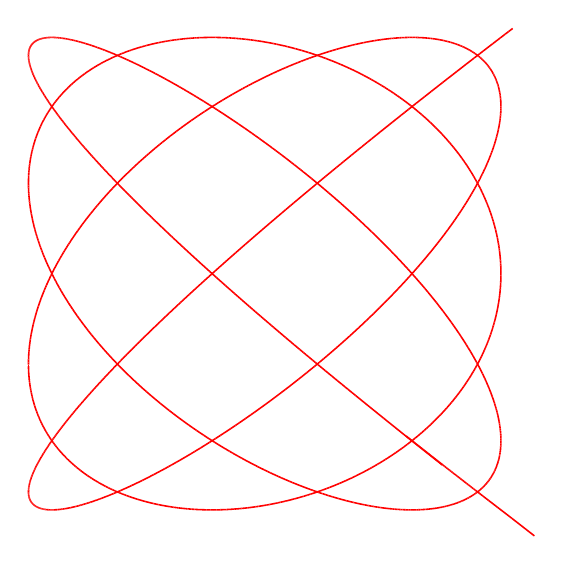
\begin{tikzpicture}[scale=1.5]
\draw[color=red,line width=.2mm] (2.0908361532717614,-2.070068484879813) --(2.283388105366839,-2.2201692178485675);
\draw[color=red,line width=.2mm] (1.9698380680294338,-1.9771216137403078) --(2.0908361532717614,-2.070068484879813);
\draw[color=red,line width=.2mm] (1.8942636790187775,-1.918966326096486) --(1.9698380680294338,-1.9771216137403078);
\draw[color=red,line width=.2mm] (1.8470576214416856,-1.8825832001305483) --(1.8942636790187775,-1.918966326096486);
\draw[color=red,line width=.2mm] (1.817564990335865,-1.8598293454375543) --(1.8470576214416856,-1.8825832001305483);
\draw[color=red,line width=.2mm] (1.7991364776100005,-1.8456025303287038) --(1.817564990335865,-1.8598293454375543);
\draw[color=red,line width=.2mm] (1.7876203744371124,-1.836708554413585) --(1.7991364776100005,-1.8456025303287038);
\draw[color=red,line width=.2mm] (1.7804234821733713,-1.8311489518870296) --(1.7876203744371124,-1.836708554413585);
\draw[color=red,line width=.2mm] (1.7714270838349806,-1.8241998144538552) --(1.7804234821733713,-1.8311489518870296);
\draw[color=red,line width=.2mm] (1.76580512421444,-1.8198555845775921) --(1.7714270838349806,-1.8241998144538552);
\draw[color=red,line width=.2mm] (1.7587782929846985,-1.8144244993050744) --(1.76580512421444,-1.8198555845775921);
\draw[color=red,line width=.2mm] (1.7499973961443995,-1.8076322341192748) --(1.7587782929846985,-1.8144244993050744);
\draw[color=red,line width=.2mm] (1.7445090487347694,-1.8033874386439368) --(1.7499973961443995,-1.8076322341192748);
\draw[color=red,line width=.2mm] (1.737649208239658,-1.7980806787244021) --(1.7445090487347694,-1.8033874386439368);
\draw[color=red,line width=.2mm] (1.7290753371494074,-1.7914460306501971) --(1.737649208239658,-1.7980806787244021);
\draw[color=red,line width=.2mm] (1.723719200322698,-1.7872961125392954) --(1.7290753371494074,-1.7914460306501971);
\draw[color=red,line width=.2mm] (1.7170223455032185,-1.7821108843039266) --(1.723719200322698,-1.7872961125392954);
\draw[color=red,line width=.2mm] (1.7086521694882975,-1.7756281995754601) --(1.7170223455032185,-1.7821108843039266);
\draw[color=red,line width=.2mm] (1.7034215083854933,-1.7715756218129481) --(1.7086521694882975,-1.7756281995754601);
\draw[color=red,line width=.2mm] (1.6968837293877312,-1.7665091950912628) --(1.7034215083854933,-1.7715756218129481);
\draw[color=red,line width=.2mm] (1.688714074413038,-1.7601728566379748) --(1.6968837293877312,-1.7665091950912628);
\draw[color=red,line width=.2mm] (1.6836076424641788,-1.756213156787777) --(1.688714074413038,-1.7601728566379748);
\draw[color=red,line width=.2mm] (1.6772251279970705,-1.751262856241558) --(1.6836076424641788,-1.756213156787777);
\draw[color=red,line width=.2mm] (1.6692478074386434,-1.7450739230862264) --(1.6772251279970705,-1.751262856241558);
\draw[color=red,line width=.2mm] (1.6642642231340086,-1.7412029599375296) --(1.6692478074386434,-1.7450739230862264);
\draw[color=red,line width=.2mm] (1.6580332524869528,-1.7363661710961025) --(1.6642642231340086,-1.7412029599375296);
\draw[color=red,line width=.2mm] (1.6502453286554828,-1.7303191709146948) --(1.6580332524869528,-1.7363661710961025);
\draw[color=red,line width=.2mm] (1.6405116601576655,-1.722758833087864) --(1.6502453286554828,-1.7303191709146948);
\draw[color=red,line width=.2mm] (1.6344308775553866,-1.7180300792382084) --(1.6405116601576655,-1.722758833087864);
\draw[color=red,line width=.2mm] (1.626828420825366,-1.7121210345350695) --(1.6344308775553866,-1.7180300792382084);
\draw[color=red,line width=.2mm] (1.6173265382822657,-1.7047332041778556) --(1.626828420825366,-1.7121210345350695);
\draw[color=red,line width=.2mm] (1.6113887926384982,-1.7001146164101977) --(1.6173265382822657,-1.7047332041778556);
\draw[color=red,line width=.2mm] (1.6039691614173985,-1.6943381120702088) --(1.6113887926384982,-1.7001146164101977);
\draw[color=red,line width=.2mm] (1.5946934905228116,-1.6871189326570042) --(1.6039691614173985,-1.6943381120702088);
\draw[color=red,line width=.2mm] (1.588897090907762,-1.6826057993788808) --(1.5946934905228116,-1.6871189326570042);
\draw[color=red,line width=.2mm] (1.5816522923593592,-1.6769634851080482) --(1.588897090907762,-1.6826057993788808);
\draw[color=red,line width=.2mm] (1.5725992908056103,-1.669906756245777) --(1.5816522923593592,-1.6769634851080482);
\draw[color=red,line width=.2mm] (1.5669408394278788,-1.6654967174691675) --(1.5725992908056103,-1.669906756245777);
\draw[color=red,line width=.2mm] (1.5598684487548888,-1.6599833072957253) --(1.5669408394278788,-1.6654967174691675);
\draw[color=red,line width=.2mm] (1.5510290150070343,-1.653090195776616) --(1.5598684487548888,-1.6599833072957253);
\draw[color=red,line width=.2mm] (1.5455072428426955,-1.648778327222099) --(1.5510290150070343,-1.653090195776616);
\draw[color=red,line width=.2mm] (1.5386031172297456,-1.6433909336481614) --(1.5455072428426955,-1.648778327222099);
\draw[color=red,line width=.2mm] (1.5299739733807227,-1.6366553971174207) --(1.5386031172297456,-1.6433909336481614);
\draw[color=red,line width=.2mm] (1.5245815520222965,-1.6324446731983124) --(1.5299739733807227,-1.6366553971174207);
\draw[color=red,line width=.2mm] (1.5178416469558011,-1.6271804745518894) --(1.5245815520222965,-1.6324446731983124);
\draw[color=red,line width=.2mm] (1.5094196831446243,-1.6205965023319404) --(1.5178416469558011,-1.6271804745518894);
\draw[color=red,line width=.2mm] (1.5041555045363815,-1.616482095802216) --(1.5094196831446243,-1.6205965023319404);
\draw[color=red,line width=.2mm] (1.4975758783542064,-1.611338325961619) --(1.5041555045363815,-1.616482095802216);
\draw[color=red,line width=.2mm] (1.4893522803857389,-1.6049074215361558) --(1.4975758783542064,-1.611338325961619);
\draw[color=red,line width=.2mm] (1.4842150790014,-1.6008848591101676) --(1.4893522803857389,-1.6049074215361558);
\draw[color=red,line width=.2mm] (1.4777918835634718,-1.5958588150603292) --(1.4842150790014,-1.6008848591101676);
\draw[color=red,line width=.2mm] (1.4697637869564866,-1.589575116201471) --(1.4777918835634718,-1.5958588150603292);
\draw[color=red,line width=.2mm] (1.464746929584488,-1.5856469089754293) --(1.4697637869564866,-1.589575116201471);
\draw[color=red,line width=.2mm] (1.4584764084966984,-1.580735948807422) --(1.464746929584488,-1.5856469089754293);
\draw[color=red,line width=.2mm] (1.450640841194672,-1.5745939593936538) --(1.4584764084966984,-1.580735948807422);
\draw[color=red,line width=.2mm] (1.445743211778347,-1.5707557251135316) --(1.450640841194672,-1.5745939593936538);
\draw[color=red,line width=.2mm] (1.4396217036846628,-1.5659572596793558) --(1.445743211778347,-1.5707557251135316);
\draw[color=red,line width=.2mm] (1.4319706461540773,-1.5599581253013828) --(1.4396217036846628,-1.5659572596793558);
\draw[color=red,line width=.2mm] (1.4224081203422552,-1.5524575593866698) --(1.4319706461540773,-1.5599581253013828);
\draw[color=red,line width=.2mm] (1.4164349799746532,-1.5477653365284638) --(1.4224081203422552,-1.5524575593866698);
\draw[color=red,line width=.2mm] (1.4089663250178286,-1.541902891044652) --(1.4164349799746532,-1.5477653365284638);
\draw[color=red,line width=.2mm] (1.3996317526368178,-1.534573251282254) --(1.4089663250178286,-1.541902891044652);
\draw[color=red,line width=.2mm] (1.3937986213614941,-1.5299909867501271) --(1.3996317526368178,-1.534573251282254);
\draw[color=red,line width=.2mm] (1.3865098836290763,-1.5242597598332956) --(1.3937986213614941,-1.5299909867501271);
\draw[color=red,line width=.2mm] (1.37739777375908,-1.5170972335760293) --(1.3865098836290763,-1.5242597598332956);
\draw[color=red,line width=.2mm] (1.3717036438640295,-1.512619464107614) --(1.37739777375908,-1.5170972335760293);
\draw[color=red,line width=.2mm] (1.364586717096397,-1.5070213197107611) --(1.3717036438640295,-1.512619464107614);
\draw[color=red,line width=.2mm] (1.355693703540183,-1.5000196539042392) --(1.364586717096397,-1.5070213197107611);
\draw[color=red,line width=.2mm] (1.3501352287876012,-1.4956440454803055) --(1.355693703540183,-1.5000196539042392);
\draw[color=red,line width=.2mm] (1.3431878424202868,-1.490173639492732) --(1.3501352287876012,-1.4956440454803055);
\draw[color=red,line width=.2mm] (1.334504716652133,-1.483334230256146) --(1.3431878424202868,-1.490173639492732);
\draw[color=red,line width=.2mm] (1.3290807806404428,-1.479055781094763) --(1.334504716652133,-1.483334230256146);
\draw[color=red,line width=.2mm] (1.3222988549248496,-1.473710257575334) --(1.3290807806404428,-1.479055781094763);
\draw[color=red,line width=.2mm] (1.3138225118467213,-1.4670270074004417) --(1.3222988549248496,-1.473710257575334);
\draw[color=red,line width=.2mm] (1.3085256309366615,-1.4628489222506298) --(1.3138225118467213,-1.4670270074004417);
\draw[color=red,line width=.2mm] (1.3019051828204153,-1.4576254904942028) --(1.3085256309366615,-1.4628489222506298);
\draw[color=red,line width=.2mm] (1.2936326876815876,-1.451092328644771) --(1.3019051828204153,-1.4576254904942028);
\draw[color=red,line width=.2mm] (1.2884619044111068,-1.4470097012527527) --(1.2936326876815876,-1.451092328644771);
\draw[color=red,line width=.2mm] (1.281999052763242,-1.4419056248126902) --(1.2884619044111068,-1.4470097012527527);
\draw[color=red,line width=.2mm] (1.273921470588374,-1.435524289270665) --(1.281999052763242,-1.4419056248126902);
\draw[color=red,line width=.2mm] (1.2688756591572827,-1.4315325767322706) --(1.273921470588374,-1.435524289270665);
\draw[color=red,line width=.2mm] (1.262566614837698,-1.4265451817062333) --(1.2688756591572827,-1.4315325767322706);
\draw[color=red,line width=.2mm] (1.2546812531795648,-1.4203097478672757) --(1.262566614837698,-1.4265451817062333);
\draw[color=red,line width=.2mm] (1.2497536413002093,-1.4164116699732283) --(1.2546812531795648,-1.4203097478672757);
\draw[color=red,line width=.2mm] (1.2435947054618786,-1.4115383429677735) --(1.2497536413002093,-1.4164116699732283);
\draw[color=red,line width=.2mm] (1.2358987530620653,-1.4054432611920198) --(1.2435947054618786,-1.4115383429677735);
\draw[color=red,line width=.2mm] (1.2262779719795962,-1.3978254681311508) --(1.2358987530620653,-1.4054432611920198);
\draw[color=red,line width=.2mm] (1.2202660965508163,-1.393062946738797) --(1.2262779719795962,-1.3978254681311508);
\draw[color=red,line width=.2mm] (1.2127539377698393,-1.3871064161566216) --(1.2202660965508163,-1.393062946738797);
\draw[color=red,line width=.2mm] (1.2033628418765852,-1.3796618823208142) --(1.2127539377698393,-1.3871064161566216);
\draw[color=red,line width=.2mm] (1.1974944774906258,-1.3750077026437302) --(1.2033628418765852,-1.3796618823208142);
\draw[color=red,line width=.2mm] (1.197857150933243,-1.3772372161353974) --(1.5037847149568087,-1.6200851723888068);
\draw[color=red,line width=.2mm] (1.007524509226037,-1.2243730556952759) --(1.197857150933243,-1.3772372161353974);
\draw[color=red,line width=.2mm] (0.888849328796528,-1.1284858094943249) --(1.007524509226037,-1.2243730556952759);
\draw[color=red,line width=.2mm] (0.8147852855345248,-1.0684241737803961) --(0.888849328796528,-1.1284858094943249);
\draw[color=red,line width=.2mm] (0.7685378452227664,-1.0308335884694801) --(0.8147852855345248,-1.0684241737803961);
\draw[color=red,line width=.2mm] (0.7396499868966117,-1.0073189545322194) --(0.7685378452227664,-1.0308335884694801);
\draw[color=red,line width=.2mm] (0.7035432421444666,-0.9779219347452535) --(0.7396499868966117,-1.0073189545322194);
\draw[color=red,line width=.2mm] (0.6810058320070184,-0.9595129733325741) --(0.7035432421444666,-0.9779219347452535);
\draw[color=red,line width=.2mm] (0.6528362792951143,-0.9364990954921883) --(0.6810058320070184,-0.9595129733325741);
\draw[color=red,line width=.2mm] (0.6176510805666208,-0.9076991610605539) --(0.6528362792951143,-0.9364990954921883);
\draw[color=red,line width=.2mm] (0.5956894773611928,-0.8896637662233396) --(0.6176510805666208,-0.9076991610605539);
\draw[color=red,line width=.2mm] (0.5682396692230776,-0.8671168783823892) --(0.5956894773611928,-0.8896637662233396);
\draw[color=red,line width=.2mm] (0.5339539455452261,-0.8389011090208548) --(0.5682396692230776,-0.8671168783823892);
\draw[color=red,line width=.2mm] (0.5125542931080062,-0.8212312796107932) --(0.5339539455452261,-0.8389011090208548);
\draw[color=red,line width=.2mm] (0.4858069089861275,-0.7991413806781692) --(0.5125542931080062,-0.8212312796107932);
\draw[color=red,line width=.2mm] (0.4523990183269603,-0.7714972629901731) --(0.4858069089861275,-0.7991413806781692);
\draw[color=red,line width=.2mm] (0.4315477998815374,-0.754185165038453) --(0.4523990183269603,-0.7714972629901731);
\draw[color=red,line width=.2mm] (0.4054859445506796,-0.732542461572222) --(0.4315477998815374,-0.754185165038453);
\draw[color=red,line width=.2mm] (0.3729347765741166,-0.7054577418771933) --(0.4054859445506796,-0.732542461572222);
\draw[color=red,line width=.2mm] (0.3526188076859486,-0.688495703909775) --(0.3729347765741166,-0.7054577418771933);
\draw[color=red,line width=.2mm] (0.32722600135389096,-0.6672906055967878) --(0.3526188076859486,-0.688495703909775);
\draw[color=red,line width=.2mm] (0.2955109650504231,-0.6407532842774594) --(0.32722600135389096,-0.6672906055967878);
\draw[color=red,line width=.2mm] (0.2757173859072991,-0.6241337937727166) --(0.2955109650504231,-0.6407532842774594);
\draw[color=red,line width=.2mm] (0.2509775545664432,-0.6033569089998554) --(0.2757173859072991,-0.6241337937727166);
\draw[color=red,line width=.2mm] (0.2200785662033224,-0.57735523495762) --(0.2509775545664432,-0.6033569089998554);
\draw[color=red,line width=.2mm] (0.20079483409614426,-0.5610709348713625) --(0.2200785662033224,-0.57735523495762);
\draw[color=red,line width=.2mm] (0.17669230012560516,-0.540713066380996) --(0.20079483409614426,-0.5610709348713625);
\draw[color=red,line width=.2mm] (0.14658977151070965,-0.5152355315963939) --(0.17669230012560516,-0.540713066380996);
\draw[color=red,line width=.2mm] (0.12780365351099784,-0.499279216952449) --(0.14658977151070965,-0.5152355315963939);
\draw[color=red,line width=.2mm] (0.1043231265246708,-0.4793313575798155) --(0.12780365351099784,-0.499279216952449);
\draw[color=red,line width=.2mm] (0.07499795357849437,-0.45436669177528416) --(0.1043231265246708,-0.4793313575798155);
\draw[color=red,line width=.2mm] (0.05669751940921306,-0.4387313063198213) --(0.07499795357849437,-0.45436669177528416);
\draw[color=red,line width=.2mm] (0.03382408734556751,-0.4191846348100653) --(0.05669751940921306,-0.4387313063198213);
\draw[color=red,line width=.2mm] (0.005257638976083995,-0.39472180021208775) --(0.03382408734556751,-0.4191846348100653);
\draw[color=red,line width=.2mm] (-0.012568745927422437,-0.37940043312987093) --(0.005257638976083995,-0.39472180021208775);
\draw[color=red,line width=.2mm] (-0.03484962547782479,-0.3602463100324647) --(-0.012568745927422437,-0.37940043312987093);
\draw[color=red,line width=.2mm] (-0.06267551820235472,-0.336274496230254) --(-0.03484962547782479,-0.3602463100324647);
\draw[color=red,line width=.2mm] (-0.08003919944431785,-0.32126037892100695) --(-0.06267551820235472,-0.336274496230254);
\draw[color=red,line width=.2mm] (-0.10174170767732671,-0.30249034255928353) --(-0.08003919944431785,-0.32126037892100695);
\draw[color=red,line width=.2mm] (-0.12884476206221265,-0.2789989614571382) --(-0.10174170767732671,-0.30249034255928353);
\draw[color=red,line width=.2mm] (-0.1457568028540797,-0.2642854643702036) --(-0.12884476206221265,-0.2789989614571382);
\draw[color=red,line width=.2mm] (-0.16689476795996067,-0.24589122688372356) --(-0.1457568028540797,-0.2642854643702036);
\draw[color=red,line width=.2mm] (-0.19329225992886642,-0.22286990774418008) --(-0.16689476795996067,-0.24589122688372356);
\draw[color=red,line width=.2mm] (-0.20976344747519007,-0.20845053726964452) --(-0.19329225992886642,-0.22286990774418008);
\draw[color=red,line width=.2mm] (-0.2303503526193286,-0.19042398072710942) --(-0.20976344747519007,-0.20845053726964452);
\draw[color=red,line width=.2mm] (-0.25605912667388636,-0.1678625653020014) --(-0.2303503526193286,-0.19042398072710942);
\draw[color=red,line width=.2mm] (-0.2881554884263532,-0.13961594752666323) --(-0.25605912667388636,-0.1678625653020014);
\draw[color=red,line width=.2mm] (-0.30817241049123795,-0.12191294184400835) --(-0.2881554884263532,-0.13961594752666323);
\draw[color=red,line width=.2mm] (-0.333190098993147,-0.09978032879082385) --(-0.30817241049123795,-0.12191294184400835);
\draw[color=red,line width=.2mm] (-0.36442242756442134,-0.07206988502401732) --(-0.333190098993147,-0.09978032879082385);
\draw[color=red,line width=.2mm] (-0.38389897072746193,-0.05470199336095968) --(-0.36442242756442134,-0.07206988502401732);
\draw[color=red,line width=.2mm] (-0.40824114431178427,-0.03298826058553629) --(-0.38389897072746193,-0.05470199336095968);
\draw[color=red,line width=.2mm] (-0.423427482404829,-0.01938653536401893) --(-0.40824114431178427,-0.03298826058553629);
\draw[color=red,line width=.2mm] (-0.4424082849684876,-0.0023820458079030567) --(-0.423427482404829,-0.01938653536401893);
\draw[color=red,line width=.2mm] (-0.46610908701719894,0.01890151406802288) --(-0.4424082849684876,-0.0023820458079030567);
\draw[color=red,line width=.2mm] (-0.49569490197738253,0.04555040978572477) --(-0.46610908701719894,0.01890151406802288);
\draw[color=red,line width=.2mm] (-0.514142054540137,0.062254434161235245) --(-0.49569490197738253,0.04555040978572477);
\draw[color=red,line width=.2mm] (-0.5371974437086131,0.08313832120277785) --(-0.514142054540137,0.062254434161235245);
\draw[color=red,line width=.2mm] (-0.5659762132826863,0.10928753911565514) --(-0.5371974437086131,0.08313832120277785);
\draw[color=red,line width=.2mm] (-0.5839184816356704,0.12567935679463466) --(-0.5659762132826863,0.10928753911565514);
\draw[color=red,line width=.2mm] (-0.6063427120513074,0.14617300705326994) --(-0.5839184816356704,0.12567935679463466);
\draw[color=red,line width=.2mm] (-0.6203297857900377,0.15901202474330134) --(-0.6063427120513074,0.14617300705326994);
\draw[color=red,line width=.2mm] (-0.6378114472071513,0.1750631357227329) --(-0.6203297857900377,0.15901202474330134);
\draw[color=red,line width=.2mm] (-0.6596377834445246,0.19515486002707164) --(-0.6378114472071513,0.1750631357227329);
\draw[color=red,line width=.2mm] (-0.6868796159910145,0.22031381596800398) --(-0.6596377834445246,0.19515486002707164);
\draw[color=red,line width=.2mm] (-0.7038607453163749,0.23608650779559343) --(-0.6868796159910145,0.22031381596800398);
\draw[color=red,line width=.2mm] (-0.7250834826877254,0.2558062569089481) --(-0.7038607453163749,0.23608650779559343);
\draw[color=red,line width=.2mm] (-0.7383192428799644,0.26816147762729975) --(-0.7250834826877254,0.2558062569089481);
\draw[color=red,line width=.2mm] (-0.7548617201240059,0.2836078460136144) --(-0.7383192428799644,0.26816147762729975);
\draw[color=red,line width=.2mm] (-0.7755137024560689,0.3029435628580748) --(-0.7548617201240059,0.2836078460136144);
\draw[color=red,line width=.2mm] (-0.7883926189930297,0.3150586560282844) --(-0.7755137024560689,0.3029435628580748);
\draw[color=red,line width=.2mm] (-0.8044890319441683,0.33020485631911645) --(-0.7883926189930297,0.3150586560282844);
\draw[color=red,line width=.2mm] (-0.8245833826275528,0.34916519825432374) --(-0.8044890319441683,0.33020485631911645);
\draw[color=red,line width=.2mm] (-0.8371137163291776,0.36104550756450143) --(-0.8245833826275528,0.34916519825432374);
\draw[color=red,line width=.2mm] (-0.8527743907950728,0.37589821914613775) --(-0.8371137163291776,0.36104550756450143);
\draw[color=red,line width=.2mm] (-0.8723240011332325,0.39449154822288246) --(-0.8527743907950728,0.37589821914613775);
\draw[color=red,line width=.2mm] (-0.8967190911388094,0.41777691853864063) --(-0.8723240011332325,0.39449154822288246);
\draw[color=red,line width=.2mm] (-0.9119200303500491,0.43237801787041874) --(-0.8967190911388094,0.41777691853864063);
\draw[color=red,line width=.2mm] (-0.9309174016914755,0.45063327219902505) --(-0.9119200303500491,0.43237801787041874);
\draw[color=red,line width=.2mm] (-0.9427616282357887,0.4620728526193147) --(-0.9309174016914755,0.45063327219902505);
\draw[color=red,line width=.2mm] (-0.9575646099116781,0.4763746679882543) --(-0.9427616282357887,0.4620728526193147);
\draw[color=red,line width=.2mm] (-0.9760415487324008,0.49427942913550676) --(-0.9575646099116781,0.4763746679882543);
\draw[color=red,line width=.2mm] (-0.9875602888008135,0.5054999136896832) --(-0.9760415487324008,0.49427942913550676);
\draw[color=red,line width=.2mm] (-1.0019563942169345,0.5195278566427647) --(-0.9875602888008135,0.5054999136896832);
\draw[color=red,line width=.2mm] (-1.0199246018655437,0.537090175203588) --(-1.0019563942169345,0.5195278566427647);
\draw[color=red,line width=.2mm] (-1.0311252274068778,0.5480965278904099) --(-1.0199246018655437,0.537090175203588);
\draw[color=red,line width=.2mm] (-1.0451236709188854,0.5618568033078362) --(-1.0311252274068778,0.5480965278904099);
\draw[color=red,line width=.2mm] (-1.0625946447691774,0.5790844498055777) --(-1.0451236709188854,0.5618568033078362);
\draw[color=red,line width=.2mm] (-1.0734843186097138,0.5898815431519241) --(-1.0625946447691774,0.5790844498055777);
\draw[color=red,line width=.2mm] (-1.0870940515765783,0.6033802431289924) --(-1.0734843186097138,0.5898815431519241);
\draw[color=red,line width=.2mm] (-1.104078959034599,0.6202808475013739) --(-1.0870940515765783,0.6033802431289924);
\draw[color=red,line width=.2mm] (-1.1146646363880774,0.630873466610576) --(-1.104078959034599,0.6202808475013739);
\draw[color=red,line width=.2mm] (-1.1278943505048753,0.6441165740183593) --(-1.1146646363880774,0.630873466610576);
\draw[color=red,line width=.2mm] (-1.1444040330547476,0.6606976301043354) --(-1.1278943505048753,0.6441165740183593);
\draw[color=red,line width=.2mm] (-1.1546924639038387,0.6710904755108191) --(-1.1444040330547476,0.6606976301043354);
\draw[color=red,line width=.2mm] (-1.1675505941621644,0.6840838675704527) --(-1.1546924639038387,0.6710904755108191);
\draw[color=red,line width=.2mm] (-1.1835955709224817,0.7003527376265238) --(-1.1675505941621644,0.6840838675704527);
\draw[color=red,line width=.2mm] (-1.1935933020761962,0.7105504281733585) --(-1.1835955709224817,0.7003527376265238);
\draw[color=red,line width=.2mm] (-1.2060880293173446,0.7232998800595658) --(-1.1935933020761962,0.7105504281733585);
\draw[color=red,line width=.2mm] (-1.2216785000705146,0.7392637993169866) --(-1.2060880293173446,0.7232998800595658);
\draw[color=red,line width=.2mm] (-1.231391876871349,0.7492708750639498) --(-1.2216785000705146,0.7392637993169866);
\draw[color=red,line width=.2mm] (-1.2435311298991736,0.7617820635473941) --(-1.231391876871349,0.7492708750639498);
\draw[color=red,line width=.2mm] (-1.2586769775496145,0.7774481448227365) --(-1.2435311298991736,0.7617820635473941);
\draw[color=red,line width=.2mm] (-1.268112145199674,0.7872690699932235) --(-1.2586769775496145,0.7774481448227365);
\draw[color=red,line width=.2mm] (-1.2799036024142663,0.799547577132177) --(-1.268112145199674,0.7872690699932235);
\draw[color=red,line width=.2mm] (-1.2946143948236624,0.8149228155048892) --(-1.2799036024142663,0.799547577132177);
\draw[color=red,line width=.2mm] (-1.3037772992936159,0.8245619814807873) --(-1.2946143948236624,0.8149228155048892);
\draw[color=red,line width=.2mm] (-1.31522838980015,0.8366132983736169) --(-1.3037772992936159,0.8245619814807873);
\draw[color=red,line width=.2mm] (-1.3295133809388828,0.8517045759455286) --(-1.31522838980015,0.8366132983736169);
\draw[color=red,line width=.2mm] (-1.3384097694172374,0.8611663043200575) --(-1.3295133809388828,0.8517045759455286);
\draw[color=red,line width=.2mm] (-1.3495276735562567,0.8729958349311313) --(-1.3384097694172374,0.8611663043200575);
\draw[color=red,line width=.2mm] (-1.36339580389935,0.8878099256842943) --(-1.3495276735562567,0.8729958349311313);
\draw[color=red,line width=.2mm] (-1.372031224731948,0.8970984713837689) --(-1.36339580389935,0.8878099256842943);
\draw[color=red,line width=.2mm] (-1.3828228739677952,0.9087115364566026) --(-1.372031224731948,0.8970984713837689);
\draw[color=red,line width=.2mm] (-1.3962827700508602,0.9232551112274272) --(-1.3828228739677952,0.9087115364566026);
\draw[color=red,line width=.2mm] (-1.4046625721114658,0.9323746657139461) --(-1.3962827700508602,0.9232551112274272);
\draw[color=red,line width=.2mm] (-1.4151346482041038,0.9437765067867222) --(-1.4046625721114658,0.9323746657139461);
\draw[color=red,line width=.2mm] (-1.428194621239429,0.9580561383760711) --(-1.4151346482041038,0.9437765067867222);
\draw[color=red,line width=.2mm] (-1.4363239526614218,0.9670108329442452) --(-1.428194621239429,0.9580561383760711);
\draw[color=red,line width=.2mm] (-1.446482886033175,0.9782066164842521) --(-1.4363239526614218,0.9670108329442452);
\draw[color=red,line width=.2mm] (-1.4591509294676592,0.9922287849249585) --(-1.446482886033175,0.9782066164842521);
\draw[color=red,line width=.2mm] (-1.4670347356538116,1.0010226941069738) --(-1.4591509294676592,0.9922287849249585);
\draw[color=red,line width=.2mm] (-1.4768867028460333,1.0120175157819955) --(-1.4670347356538116,1.0010226941069738);
\draw[color=red,line width=.2mm] (-1.4891704887204327,1.0257886137871652) --(-1.4768867028460333,1.0120175157819955);
\draw[color=red,line width=.2mm] (-1.4968135095319728,1.0344257588816776) --(-1.4891704887204327,1.0257886137871652);
\draw[color=red,line width=.2mm] (-1.5063644296266612,1.0452246479878875) --(-1.4968135095319728,1.0344257588816776);
\draw[color=red,line width=.2mm] (-1.5182713035687003,1.0587509866052562) --(-1.5063644296266612,1.0452246479878875);
\draw[color=red,line width=.2mm] (-1.525678069575708,1.0672353393468061) --(-1.5182713035687003,1.0587509866052562);
\draw[color=red,line width=.2mm] (-1.534933599432827,1.0778432634142203) --(-1.525678069575708,1.0672353393468061);
\draw[color=red,line width=.2mm] (-1.5464705740839615,1.09113107791368) --(-1.534933599432827,1.0778432634142203);
\draw[color=red,line width=.2mm] (-1.553645401735787,1.0994665643004087) --(-1.5464705740839615,1.09113107791368);
\draw[color=red,line width=.2mm] (-1.5626109298674202,1.1098884338983295) --(-1.553645401735787,1.0994665643004087);
\draw[color=red,line width=.2mm] (-1.5737846765030012,1.1229438899213722) --(-1.5626109298674202,1.1098884338983295);
\draw[color=red,line width=.2mm] (-1.580731662048754,1.1311343942196952) --(-1.5737846765030012,1.1229438899213722);
\draw[color=red,line width=.2mm] (-1.5894123009148997,1.14137506798568) --(-1.580731662048754,1.1311343942196952);
\draw[color=red,line width=.2mm] (-1.6002291389683054,1.1542042679866893) --(-1.5894123009148997,1.14137506798568);
\draw[color=red,line width=.2mm] (-1.6069521509221858,1.162253636932067) --(-1.6002291389683054,1.1542042679866893);
\draw[color=red,line width=.2mm] (-1.6153527273882375,1.172317926848541) --(-1.6069521509221858,1.162253636932067);
\draw[color=red,line width=.2mm] (-1.625818611528818,1.184926916858265) --(-1.6153527273882375,1.172317926848541);
\draw[color=red,line width=.2mm] (-1.632321281431388,1.1928389640709927) --(-1.625818611528818,1.184926916858265);
\draw[color=red,line width=.2mm] (-1.6404463250718844,1.2027316410133393) --(-1.632321281431388,1.1928389640709927);
\draw[color=red,line width=.2mm] (-1.6505668294112115,1.2151264177539607) --(-1.6404463250718844,1.2027316410133393);
\draw[color=red,line width=.2mm] (-1.6568525405833299,1.2229049283875915) --(-1.6505668294112115,1.2151264177539607);
\draw[color=red,line width=.2mm] (-1.6647062694474999,1.232630727965848) --(-1.6568525405833299,1.2229049283875915);
\draw[color=red,line width=.2mm] (-1.6744865683544048,1.2448172463440472) --(-1.6647062694474999,1.232630727965848);
\draw[color=red,line width=.2mm] (-1.6805584422724993,1.2524659819809936) --(-1.6744865683544048,1.2448172463440472);
\draw[color=red,line width=.2mm] (-1.6881447456406389,1.2620296106933353) --(-1.6805584422724993,1.2524659819809936);
\draw[color=red,line width=.2mm] (-1.6975895905275507,1.2740137916914231) --(-1.6881447456406389,1.2620296106933353);
\draw[color=red,line width=.2mm] (-1.7034504703632465,1.281536495494515) --(-1.6975895905275507,1.2740137916914231);
\draw[color=red,line width=.2mm] (-1.7107728879140371,1.2909426372033062) --(-1.7034504703632465,1.281536495494515);
\draw[color=red,line width=.2mm] (-1.7198865792082778,1.3027303761771079) --(-1.7107728879140371,1.2909426372033062);
\draw[color=red,line width=.2mm] (-1.725539009966938,1.3101307782959675) --(-1.7198865792082778,1.3027303761771079);
\draw[color=red,line width=.2mm] (-1.7326007066378109,1.3193841010244356) --(-1.725539009966938,1.3101307782959675);
\draw[color=red,line width=.2mm] (-1.7413870599625296,1.3309812763974416) --(-1.7326007066378109,1.3193841010244356);
\draw[color=red,line width=.2mm] (-1.746833264517107,1.3382630996123017) --(-1.7413870599625296,1.3309812763974416);
\draw[color=red,line width=.2mm] (-1.7536370001638677,1.347368262639076) --(-1.746833264517107,1.3382630996123017);
\draw[color=red,line width=.2mm] (-1.7620993055119252,1.358780744951386) --(-1.7536370001638677,1.347368262639076);
\draw[color=red,line width=.2mm] (-1.7673411556514425,1.3659477105111535) --(-1.7620993055119252,1.358780744951386);
\draw[color=red,line width=.2mm] (-1.7738892483877713,1.3749093717067749) --(-1.7673411556514425,1.3659477105111535);
\draw[color=red,line width=.2mm] (-1.782030220761673,1.3861430329284072) --(-1.7738892483877713,1.3749093717067749);
\draw[color=red,line width=.2mm] (-1.7870692021452546,1.3931988664993604) --(-1.782030220761673,1.3861430329284072);
\draw[color=red,line width=.2mm] (-1.7933634839515429,1.402021689797014) --(-1.7870692021452546,1.3931988664993604);
\draw[color=red,line width=.2mm] (-1.801185203541284,1.4130824127388564) --(-1.7933634839515429,1.402021689797014);
\draw[color=red,line width=.2mm] (-1.8060223731521878,1.4200308503177566) --(-1.801185203541284,1.4130824127388564);
\draw[color=red,line width=.2mm] (-1.8120641359649852,1.4287195131300663) --(-1.8060223731521878,1.4200308503177566);
\draw[color=red,line width=.2mm] (-1.8195679754134062,1.4396132006677473) --(-1.8120641359649852,1.4287195131300663);
\draw[color=red,line width=.2mm] (-1.8242039097202392,1.446457994216583) --(-1.8195679754134062,1.4396132006677473);
\draw[color=red,line width=.2mm] (-1.8299938397192572,1.4550171944862191) --(-1.8242039097202392,1.446457994216583);
\draw[color=red,line width=.2mm] (-1.8335776659987952,1.460389708576178) --(-1.8299938397192572,1.4550171944862191);
\draw[color=red,line width=.2mm] (-1.8380544125990876,1.4671072808888241) --(-1.8335776659987952,1.460389708576178);
\draw[color=red,line width=.2mm] (-1.8436177058430787,1.4755254800820354) --(-1.8380544125990876,1.4671072808888241);
\draw[color=red,line width=.2mm] (-1.8470585927381253,1.4808101438845507) --(-1.8436177058430787,1.4755254800820354);
\draw[color=red,line width=.2mm] (-1.8513565393511366,1.4874179305983486) --(-1.8470585927381253,1.4808101438845507);
\draw[color=red,line width=.2mm] (-1.8566952033812603,1.4956990821237488) --(-1.8513565393511366,1.4874179305983486);
\draw[color=red,line width=.2mm] (-1.859994413604432,1.500898298030081) --(-1.8566952033812603,1.4956990821237488);
\draw[color=red,line width=.2mm] (-1.864115128724783,1.5073993017625709) --(-1.859994413604432,1.500898298030081);
\draw[color=red,line width=.2mm] (-1.8692310109196182,1.5155471710099402) --(-1.864115128724783,1.5073993017625709);
\draw[color=red,line width=.2mm] (-1.872389569218404,1.5206633051046405) --(-1.8692310109196182,1.5155471710099402);
\draw[color=red,line width=.2mm] (-1.8763343191664807,1.5270604849645186) --(-1.872389569218404,1.5206633051046405);
\draw[color=red,line width=.2mm] (-1.8812288750449258,1.5350787816191445) --(-1.8763343191664807,1.5270604849645186);
\draw[color=red,line width=.2mm] (-1.8842475448659668,1.5401141634418576) --(-1.8812288750449258,1.5350787816191445);
\draw[color=red,line width=.2mm] (-1.8880172673340396,1.5464104326803971) --(-1.8842475448659668,1.5401141634418576);
\draw[color=red,line width=.2mm] (-1.8926915252648413,1.5543028071173755) --(-1.8880172673340396,1.5464104326803971);
\draw[color=red,line width=.2mm] (-1.895570784068148,1.5592597265972914) --(-1.8926915252648413,1.5543028071173755);
\draw[color=red,line width=.2mm] (-1.8991660569224404,1.5654579486759739) --(-1.895570784068148,1.5592597265972914);
\draw[color=red,line width=.2mm] (-1.903620576468521,1.5732279861575151) --(-1.8991660569224404,1.5654579486759739);
\draw[color=red,line width=.2mm] (-1.906360586578723,1.578108688887496) --(-1.903620576468521,1.5732279861575151);
\draw[color=red,line width=.2mm] (-1.9097815910176856,1.584211671431348) --(-1.906360586578723,1.578108688887496);
\draw[color=red,line width=.2mm] (-1.9140164137334976,1.5918628833472965) --(-1.9097815910176856,1.584211671431348);
\draw[color=red,line width=.2mm] (-1.916616987896524,1.5966695636211332) --(-1.9140164137334976,1.5918628833472965);
\draw[color=red,line width=.2mm] (-1.9198634649135569,1.6026800495223423) --(-1.916616987896524,1.5966695636211332);
\draw[color=red,line width=.2mm] (-1.9238780561877664,1.6102158606427062) --(-1.9198634649135569,1.6026800495223423);
\draw[color=red,line width=.2mm] (-1.9263386168456635,1.6149506514716634) --(-1.9238780561877664,1.6102158606427062);
\draw[color=red,line width=.2mm] (-1.9294098157485733,1.620871306143154) --(-1.9263386168456635,1.6149506514716634);
\draw[color=red,line width=.2mm] (-1.9332029960267816,1.6282950364784345) --(-1.9294098157485733,1.620871306143154);
\draw[color=red,line width=.2mm] (-1.9355225271494843,1.6329599955177625) --(-1.9332029960267816,1.6282950364784345);
\draw[color=red,line width=.2mm] (-1.9384171446710132,1.6387933889314683) --(-1.9355225271494843,1.6329599955177625);
\draw[color=red,line width=.2mm] (-1.9419870081113093,1.6461082282822666) --(-1.9384171446710132,1.6387933889314683);
\draw[color=red,line width=.2mm] (-1.9441639982403813,1.6507053182042266) --(-1.9419870081113093,1.6461082282822666);
\draw[color=red,line width=.2mm] (-1.9468801065455907,1.6564538998448386) --(-1.9441639982403813,1.6507053182042266);
\draw[color=red,line width=.2mm] (-1.9502239248728566,1.6636628724116116) --(-1.9468801065455907,1.6564538998448386);
\draw[color=red,line width=.2mm] (-1.952256299857877,1.668193933716769) --(-1.9502239248728566,1.6636628724116116);
\draw[color=red,line width=.2mm] (-1.9547912615409884,1.673859997885065) --(-1.952256299857877,1.668193933716769);
\draw[color=red,line width=.2mm] (-1.9579053706161007,1.6809659133266563) --(-1.9547912615409884,1.673859997885065);
\draw[color=red,line width=.2mm] (-1.9597904143990055,1.6854326268325979) --(-1.9579053706161007,1.6809659133266563);
\draw[color=red,line width=.2mm] (-1.9621407824171477,1.691018264770241) --(-1.9597904143990055,1.6854326268325979);
\draw[color=red,line width=.2mm] (-1.9635698025484842,1.6945252706821368) --(-1.9621407824171477,1.691018264770241);
\draw[color=red,line width=.2mm] (-1.9653524560644315,1.6989103568330277) --(-1.9635698025484842,1.6945252706821368);
\draw[color=red,line width=.2mm] (-1.9675430970166254,1.7044062897749825) --(-1.9653524560644315,1.6989103568330277);
\draw[color=red,line width=.2mm] (-1.9688702972231649,1.7078570780143052) --(-1.9675430970166254,1.7044062897749825);
\draw[color=red,line width=.2mm] (-1.9705254799780947,1.7121718725807522) --(-1.9688702972231649,1.7078570780143052);
\draw[color=red,line width=.2mm] (-1.9725550120555717,1.7175797089623996) --(-1.9705254799780947,1.7121718725807522);
\draw[color=red,line width=.2mm] (-1.9737795120761286,1.7209751525600976) --(-1.9725550120555717,1.7175797089623996);
\draw[color=red,line width=.2mm] (-1.9753061096295943,1.7252207370333805) --(-1.9737795120761286,1.7209751525600976);
\draw[color=red,line width=.2mm] (-1.9771729743900381,1.7305417563203107) --(-1.9753061096295943,1.7252207370333805);
\draw[color=red,line width=.2mm] (-1.9782936127251816,1.7338825679893235) --(-1.9771729743900381,1.7305417563203107);
\draw[color=red,line width=.2mm] (-1.9796901533842184,1.738059822952185) --(-1.9782936127251816,1.7338825679893235);
\draw[color=red,line width=.2mm] (-1.9813923308218397,1.7432950349620606) --(-1.9796901533842184,1.738059822952185);
\draw[color=red,line width=.2mm] (-1.9824076410402571,1.746581736812699) --(-1.9813923308218397,1.7432950349620606);
\draw[color=red,line width=.2mm] (-1.9836722705098677,1.7506913019075363) --(-1.9824076410402571,1.746581736812699);
\draw[color=red,line width=.2mm] (-1.985207247389513,1.7558413924592422) --(-1.9836722705098677,1.7506913019075363);
\draw[color=red,line width=.2mm] (-1.9861154386484792,1.7590742769519172) --(-1.985207247389513,1.7558413924592422);
\draw[color=red,line width=.2mm] (-1.987245895929887,1.7631165014597332) --(-1.9861154386484792,1.7590742769519172);
\draw[color=red,line width=.2mm] (-1.9886106364998282,1.76818176542336) --(-1.987245895929887,1.7631165014597332);
\draw[color=red,line width=.2mm] (-1.9894095766727864,1.771360847447821) --(-1.9886106364998282,1.76818176542336);
\draw[color=red,line width=.2mm] (-1.9904031734429548,1.7753357296753505) --(-1.9894095766727864,1.771360847447821);
\draw[color=red,line width=.2mm] (-1.9915940958236085,1.7803159890802345) --(-1.9904031734429548,1.7753357296753505);
\draw[color=red,line width=.2mm] (-1.9922812998864468,1.7834409476411508) --(-1.9915940958236085,1.7803159890802345);
\draw[color=red,line width=.2mm] (-1.99313490677523,1.7873480612302703) --(-1.9922812998864468,1.7834409476411508);
\draw[color=red,line width=.2mm] (-1.9941478699505766,1.7922425660763084) --(-1.99313490677523,1.7873480612302703);
\draw[color=red,line width=.2mm] (-1.9947204975202273,1.7953126741723513) --(-1.9941478699505766,1.7922425660763084);
\draw[color=red,line width=.2mm] (-1.995430542285986,1.7991510796084547) --(-1.9947204975202273,1.7953126741723513);
\draw[color=red,line width=.2mm] (-1.9962608508353377,1.8039583893839537) --(-1.995430542285986,1.7991510796084547);
\draw[color=red,line width=.2mm] (-1.9967157184048177,1.8069724311073927) --(-1.9962608508353377,1.8039583893839537);
\draw[color=red,line width=.2mm] (-1.9972782031042464,1.8107405713010116) --(-1.9967157184048177,1.8069724311073927);
\draw[color=red,line width=.2mm] (-1.9975881731649512,1.813100893077809) --(-1.9972782031042464,1.8107405713010116);
\draw[color=red,line width=.2mm] (-1.9979719423434503,1.8160515944910354) --(-1.9975881731649512,1.813100893077809);
\draw[color=red,line width=.2mm] (-1.9984126408138876,1.8197441987472267) --(-1.9979719423434503,1.8160515944910354);
\draw[color=red,line width=.2mm] (-1.9986448141593731,1.8220562133875233) --(-1.9984126408138876,1.8197441987472267);
\draw[color=red,line width=.2mm] (-1.9989312033143218,1.8249464172868668) --(-1.9986448141593731,1.8220562133875233);
\draw[color=red,line width=.2mm] (-1.9992487705915571,1.8285622923779667) --(-1.9989312033143218,1.8249464172868668);
\draw[color=red,line width=.2mm] (-1.999402447455224,1.830825073384908) --(-1.9992487705915571,1.8285622923779667);
\draw[color=red,line width=.2mm] (-1.9995905904424442,1.8336536056654384) --(-1.999402447455224,1.830825073384908);
\draw[color=red,line width=.2mm] (-1.9997839451717698,1.8371911298493384) --(-1.9995905904424442,1.8336536056654384);
\draw[color=red,line width=.2mm] (-1.9998584626010965,1.8394034893715765) --(-1.9997839451717698,1.8371911298493384);
\draw[color=red,line width=.2mm] (-1.9999475392936799,1.8421688490001693) --(-1.9998584626010965,1.8394034893715765);
\draw[color=red,line width=.2mm] (-2.000015685343214,1.8456259796695251) --(-1.9999475392936799,1.8421688490001693);
\draw[color=red,line width=.2mm] (-2.000010467095071,1.8477864546578957) --(-2.000015685343214,1.8456259796695251);
\draw[color=red,line width=.2mm] (-1.9999997704774484,1.8504867964496776) --(-2.000010467095071,1.8477864546578957);
\draw[color=red,line width=.2mm] (-1.9999418880074797,1.8538610517692198) --(-1.9999997704774484,1.8504867964496776);
\draw[color=red,line width=.2mm] (-1.9998565095399314,1.8559678967718831) --(-1.9999418880074797,1.8538610517692198);
\draw[color=red,line width=.2mm] (-1.9997455277151175,1.858601023198021) --(-1.9998565095399314,1.8559678967718831);
\draw[color=red,line width=.2mm] (-1.9995610832198267,1.8618894769506595) --(-1.9997455277151175,1.858601023198021);
\draw[color=red,line width=.2mm] (-1.9993953486942786,1.8639406674328236) --(-1.9995610832198267,1.8618894769506595);
\draw[color=red,line width=.2mm] (-1.9991838617383109,1.8665040338489165) --(-1.9993953486942786,1.8639406674328236);
\draw[color=red,line width=.2mm] (-1.9988727363713332,1.8697033293274783) --(-1.9991838617383109,1.8665040338489165);
\draw[color=red,line width=.2mm] (-1.9986267664060005,1.87169657949418) --(-1.9988727363713332,1.8697033293274783);
\draw[color=red,line width=.2mm] (-1.998314956341649,1.8741873177425952) --(-1.9986267664060005,1.87169657949418);
\draw[color=red,line width=.2mm] (-1.9978775894263021,1.8772937070643625) --(-1.998314956341649,1.8741873177425952);
\draw[color=red,line width=.2mm] (-1.9975519165009277,1.8792265062559488) --(-1.9978775894263021,1.8772937070643625);
\draw[color=red,line width=.2mm] (-1.9971404863383064,1.881641471650744) --(-1.9975519165009277,1.8792265062559488);
\draw[color=red,line width=.2mm] (-1.9965780277718985,1.884650886624432) --(-1.9971404863383064,1.881641471650744);
\draw[color=red,line width=.2mm] (-1.9961736939092096,1.8865205577803943) --(-1.9965780277718985,1.884650886624432);
\draw[color=red,line width=.2mm] (-1.9956639888661665,1.8888564036913356) --(-1.9961736939092096,1.8865205577803943);
\draw[color=red,line width=.2mm] (-1.9949784504091683,1.8917645628998392) --(-1.9956639888661665,1.8888564036913356);
\draw[color=red,line width=.2mm] (-1.9944970993281668,1.8935683450852425) --(-1.9949784504091683,1.8917645628998392);
\draw[color=red,line width=.2mm] (-1.9938912203635355,1.8958216273848985) --(-1.9944970993281668,1.8935683450852425);
\draw[color=red,line width=.2mm] (-1.993085612139057,1.898624181111934) --(-1.9938912203635355,1.8958216273848985);
\draw[color=red,line width=.2mm] (-1.992529565992365,1.9003593355293642) --(-1.993085612139057,1.898624181111934);
\draw[color=red,line width=.2mm] (-1.9918304633001962,1.9025266459028547) --(-1.992529565992365,1.9003593355293642);
\draw[color=red,line width=.2mm] (-1.9909088991364063,1.9052193558547148) --(-1.9918304633001962,1.9025266459028547);
\draw[color=red,line width=.2mm] (-1.990281208895432,1.9068832912419476) --(-1.9909088991364063,1.9052193558547148);
\draw[color=red,line width=.2mm] (-1.9894927418673543,1.9089614139638391) --(-1.990281208895432,1.9068832912419476);
\draw[color=red,line width=.2mm] (-1.9884604965114576,1.9115403588372075) --(-1.9894927418673543,1.9089614139638391);
\draw[color=red,line width=.2mm] (-1.987764955756443,1.9131307681721814) --(-1.9884604965114576,1.9115403588372075);
\draw[color=red,line width=.2mm] (-1.9868919069685809,1.915116850074149) --(-1.987764955756443,1.9131307681721814);
\draw[color=red,line width=.2mm] (-1.9857554106646471,1.91757864192565) --(-1.9868919069685809,1.915116850074149);
\draw[color=red,line width=.2mm] (-1.9849965254226123,1.9190936388001474) --(-1.9857554106646471,1.91757864192565);
\draw[color=red,line width=.2mm] (-1.9840445599441774,1.9209853578784208) --(-1.9849965254226123,1.9190936388001474);
\draw[color=red,line width=.2mm] (-1.9828113217767396,1.923327349485878) --(-1.9840445599441774,1.9209853578784208);
\draw[color=red,line width=.2mm] (-1.981994234023893,1.924765590432861) --(-1.9828113217767396,1.923327349485878);
\draw[color=red,line width=.2mm] (-1.980969801580683,1.9265613061675886) --(-1.981994234023893,1.924765590432861);
\draw[color=red,line width=.2mm] (-1.979648261722303,1.9287817677390875) --(-1.980969801580683,1.9265613061675886);
\draw[color=red,line width=.2mm] (-1.978778630410081,1.9301425470929028) --(-1.979648261722303,1.9287817677390875);
\draw[color=red,line width=.2mm] (-1.977688815612343,1.9318414161085278) --(-1.978778630410081,1.9301425470929028);
\draw[color=red,line width=.2mm] (-1.9762881364921856,1.9339396618468383) --(-1.977688815612343,1.9318414161085278);
\draw[color=red,line width=.2mm] (-1.9753719860728267,1.9352229686778681) --(-1.9762881364921856,1.9339396618468383);
\draw[color=red,line width=.2mm] (-1.9742243193162714,1.9368250131616362) --(-1.9753719860728267,1.9352229686778681);
\draw[color=red,line width=.2mm] (-1.9727541344221962,1.9388014642822522) --(-1.9742243193162714,1.9368250131616362);
\draw[color=red,line width=.2mm] (-1.9717976853154033,1.940007996056517) --(-1.9727541344221962,1.9388014642822522);
\draw[color=red,line width=.2mm] (-1.9705999322616676,1.941514118682622) --(-1.9717976853154033,1.940007996056517);
\draw[color=red,line width=.2mm] (-1.969070076638602,1.9433702982242338) --(-1.9705999322616676,1.941514118682622);
\draw[color=red,line width=.2mm] (-1.9680795738109937,1.9445014318745575) --(-1.969070076638602,1.9433702982242338);
\draw[color=red,line width=.2mm] (-1.9668395232930849,1.9459133783531621) --(-1.9680795738109937,1.9445014318745575);
\draw[color=red,line width=.2mm] (-1.9652597706212276,1.9476518423871638) --(-1.9668395232930849,1.9459133783531621);
\draw[color=red,line width=.2mm] (-1.9642413252042867,1.9487095689735663) --(-1.9652597706212276,1.9476518423871638);
\draw[color=red,line width=.2mm] (-1.9629665937499747,1.9500298459874472) --(-1.9642413252042867,1.9487095689735663);
\draw[color=red,line width=.2mm] (-1.9613464213693683,1.9516540634581314) --(-1.9629665937499747,1.9500298459874472);
\draw[color=red,line width=.2mm] (-1.9592804226401492,1.9536430843730799) --(-1.9613464213693683,1.9516540634581314);
\draw[color=red,line width=.2mm] (-1.9579469232103628,1.95484149185526) --(-1.9592804226401492,1.9536430843730799);
\draw[color=red,line width=.2mm] (-1.956278024506639,1.9563367566011545) --(-1.9579469232103628,1.95484149185526);
\draw[color=red,line width=.2mm] (-1.954156171464693,1.958165576989677) --(-1.956278024506639,1.9563367566011545);
\draw[color=red,line width=.2mm] (-1.9527931791961157,1.9592652294765949) --(-1.954156171464693,1.958165576989677);
\draw[color=red,line width=.2mm] (-1.9510877622065632,1.960637265687319) --(-1.9527931791961157,1.9592652294765949);
\draw[color=red,line width=.2mm] (-1.9489250098942907,1.962313594362218) --(-1.9510877622065632,1.960637265687319);
\draw[color=red,line width=.2mm] (-1.9475414679289367,1.9633198252182016) --(-1.9489250098942907,1.962313594362218);
\draw[color=red,line width=.2mm] (-1.9458106533858324,1.9645752968081165) --(-1.9475414679289367,1.9633198252182016);
\draw[color=red,line width=.2mm] (-1.943620486439125,1.9661078471845226) --(-1.9458106533858324,1.9645752968081165);
\draw[color=red,line width=.2mm] (-1.9422243402588621,1.9670264547385845) --(-1.943620486439125,1.9661078471845226);
\draw[color=red,line width=.2mm] (-1.9404780087890763,1.9681725991756331) --(-1.9422243402588621,1.9670264547385845);
\draw[color=red,line width=.2mm] (-1.93827231656491,1.969570661468476) --(-1.9404780087890763,1.9681725991756331);
\draw[color=red,line width=.2mm] (-1.93687048403531,1.970407660138399) --(-1.93827231656491,1.969570661468476);
\draw[color=red,line width=.2mm] (-1.9351172396544338,1.9714519809088975) --(-1.93687048403531,1.970407660138399);
\draw[color=red,line width=.2mm] (-1.9329063081070643,1.9727250591642982) --(-1.9351172396544338,1.9714519809088975);
\draw[color=red,line width=.2mm] (-1.9301137941982736,1.9742664926456266) --(-1.9329063081070643,1.9727250591642982);
\draw[color=red,line width=.2mm] (-1.9283393620871006,1.9751770679363367) --(-1.9301137941982736,1.9742664926456266);
\draw[color=red,line width=.2mm] (-1.9261203382038568,1.9763127786663348) --(-1.9283393620871006,1.9751770679363367);
\draw[color=red,line width=.2mm] (-1.9233228350572493,1.977686461776421) --(-1.9261203382038568,1.9763127786663348);
\draw[color=red,line width=.2mm] (-1.9215505658684182,1.9784966535507005) --(-1.9233228350572493,1.977686461776421);
\draw[color=red,line width=.2mm] (-1.9193344424004093,1.9795071495725438) --(-1.9215505658684182,1.9784966535507005);
\draw[color=red,line width=.2mm] (-1.9165449072052752,1.9807283370936217) --(-1.9193344424004093,1.9795071495725438);
\draw[color=red,line width=.2mm] (-1.9147820049347026,1.9814475470883597) --(-1.9165449072052752,1.9807283370936217);
\draw[color=red,line width=.2mm] (-1.9125777428646868,1.9823445449979402) --(-1.9147820049347026,1.9814475470883597);
\draw[color=red,line width=.2mm] (-1.9098066222160943,1.983427699771857) --(-1.9125777428646868,1.9823445449979402);
\draw[color=red,line width=.2mm] (-1.9080588410662438,1.984064728198615) --(-1.9098066222160943,1.983427699771857);
\draw[color=red,line width=.2mm] (-1.9058736003996992,1.984859198031606) --(-1.9080588410662438,1.984064728198615);
\draw[color=red,line width=.2mm] (-1.9031292000268252,1.9858177792579679) --(-1.9058736003996992,1.984859198031606);
\draw[color=red,line width=.2mm] (-1.8996799060961234,1.9869633338467712) --(-1.9031292000268252,1.9858177792579679);
\draw[color=red,line width=.2mm] (-1.8975055285932165,1.9876242511648996) --(-1.8996799060961234,1.9869633338467712);
\draw[color=red,line width=.2mm] (-1.8947870986087023,1.9884481534958662) --(-1.8975055285932165,1.9876242511648996);
\draw[color=red,line width=.2mm] (-1.891374368474941,1.9894309154396312) --(-1.8947870986087023,1.9884481534958662);
\draw[color=red,line width=.2mm] (-1.889226964019983,1.9899961037181535) --(-1.891374368474941,1.9894309154396312);
\draw[color=red,line width=.2mm] (-1.886542350429461,1.9907005766567205) --(-1.889226964019983,1.9899961037181535);
\draw[color=red,line width=.2mm] (-1.8831751639616972,1.9915392104996046) --(-1.886542350429461,1.9907005766567205);
\draw[color=red,line width=.2mm] (-1.878949797059948,1.9925238922897333) --(-1.8831751639616972,1.9915392104996046);
\draw[color=red,line width=.2mm] (-1.876293143539643,1.9930733018674498) --(-1.878949797059948,1.9925238922897333);
\draw[color=red,line width=.2mm] (-1.8729720862560604,1.9937576751441815) --(-1.876293143539643,1.9930733018674498);
\draw[color=red,line width=.2mm] (-1.868808703215428,1.9945572064613608) --(-1.8729720862560604,1.9937576751441815);
\draw[color=red,line width=.2mm] (-1.8661950462821446,1.994999091967997) --(-1.868808703215428,1.9945572064613608);
\draw[color=red,line width=.2mm] (-1.8629278016331292,1.995549301143366) --(-1.8661950462821446,1.994999091967997);
\draw[color=red,line width=.2mm] (-1.8588349755747382,1.9961880110204526) --(-1.8629278016331292,1.995549301143366);
\draw[color=red,line width=.2mm] (-1.853706726489181,1.9969124758078056) --(-1.8588349755747382,1.9961880110204526);
\draw[color=red,line width=.2mm] (-1.8504902561452956,1.9972890165048185) --(-1.853706726489181,1.9969124758078056);
\draw[color=red,line width=.2mm] (-1.8464696528469757,1.9977572239389076) --(-1.8504902561452956,1.9972890165048185);
\draw[color=red,line width=.2mm] (-1.8414357922279043,1.99827841767601) --(-1.8464696528469757,1.9977572239389076);
\draw[color=red,line width=.2mm] (-1.8382822687401223,1.9985383097312686) --(-1.8414357922279043,1.99827841767601);
\draw[color=red,line width=.2mm] (-1.834340380088081,1.9988609330597482) --(-1.8382822687401223,1.9985383097312686);
\draw[color=red,line width=.2mm] (-1.8294078812622157,1.9992087302733716) --(-1.834340380088081,1.9988609330597482);
\draw[color=red,line width=.2mm] (-1.8263205200652726,1.9993689573710993) --(-1.8294078812622157,1.9992087302733716);
\draw[color=red,line width=.2mm] (-1.8224613610082832,1.9995672007563468) --(-1.8263205200652726,1.9993689573710993);
\draw[color=red,line width=.2mm] (-1.8176343872406877,1.9997667231673377) --(-1.8224613610082832,1.9995672007563468);
\draw[color=red,line width=.2mm] (-1.8146149815501413,1.9998415918755625) --(-1.8176343872406877,1.9997667231673377);
\draw[color=red,line width=.2mm] (-1.8108407890795668,1.999933317988035) --(-1.8146149815501413,1.9998415918755625);
\draw[color=red,line width=.2mm] (-1.8061215290926227,2.0000057537346754) --(-1.8108407890795668,1.999933317988035);
\draw[color=red,line width=.2mm] (-1.8002207942635924,2.0000326907488657) --(-1.8061215290926227,2.0000057537346754);
\draw[color=red,line width=.2mm] (-1.7965319369223542,1.9999839425335633) --(-1.8002207942635924,2.0000326907488657);
\draw[color=red,line width=.2mm] (-1.7919210592814683,1.9999208181451973) --(-1.7965319369223542,1.9999839425335633);
\draw[color=red,line width=.2mm] (-1.7861576006011253,1.999786781268943) --(-1.7919210592814683,1.9999208181451973);
\draw[color=red,line width=.2mm] (-1.7825562060025872,1.9996462954824097) --(-1.7861576006011253,1.999786781268943);
\draw[color=red,line width=.2mm] (-1.7780546627866212,1.9994686796924535) --(-1.7825562060025872,1.9996462954824097);
\draw[color=red,line width=.2mm] (-1.7724290708919286,1.9991988079665812) --(-1.7780546627866212,1.9994686796924535);
\draw[color=red,line width=.2mm] (-1.7689149402956255,1.9989807842119078) --(-1.7724290708919286,1.9991988079665812);
\draw[color=red,line width=.2mm] (-1.764522481833729,1.9987064139598947) --(-1.7689149402956255,1.9989807842119078);
\draw[color=red,line width=.2mm] (-1.7590340274369725,1.9983216640780097) --(-1.764522481833729,1.9987064139598947);
\draw[color=red,line width=.2mm] (-1.7521771835328632,1.9977777905232144) --(-1.7590340274369725,1.9983216640780097);
\draw[color=red,line width=.2mm] (-1.747896185173451,1.9973729967655751) --(-1.7521771835328632,1.9977777905232144);
\draw[color=red,line width=.2mm] (-1.74254528080877,1.9968648200019317) --(-1.747896185173451,1.9973729967655751);
\draw[color=red,line width=.2mm] (-1.7358612183636426,1.9961750674670051) --(-1.74254528080877,1.9968648200019317);
\draw[color=red,line width=.2mm] (-1.731688912595286,1.9956878664138757) --(-1.7358612183636426,1.9961750674670051);
\draw[color=red,line width=.2mm] (-1.726473866525681,1.9950768519601705) --(-1.731688912595286,1.9956878664138757);
\draw[color=red,line width=.2mm] (-1.7199600675669766,1.9942657254692469) --(-1.726473866525681,1.9950768519601705);
\draw[color=red,line width=.2mm] (-1.7118259288727224,1.9931806376587091) --(-1.7199600675669766,1.9942657254692469);
\draw[color=red,line width=.2mm] (-1.7067511858117779,1.9924292397820942) --(-1.7118259288727224,1.9931806376587091);
\draw[color=red,line width=.2mm] (-1.7004082590781489,1.9914876219510116) --(-1.7067511858117779,1.9924292397820942);
\draw[color=red,line width=.2mm] (-1.6924880481863767,1.9902492277852668) --(-1.7004082590781489,1.9914876219510116);
\draw[color=red,line width=.2mm] (-1.6875471690992336,1.9894122019320615) --(-1.6924880481863767,1.9902492277852668);
\draw[color=red,line width=.2mm] (-1.6813715533595737,1.9883637215015308) --(-1.6875471690992336,1.9894122019320615);
\draw[color=red,line width=.2mm] (-1.6736604643309985,1.9870000370874488) --(-1.6813715533595737,1.9883637215015308);
\draw[color=red,line width=.2mm] (-1.6688501694549416,1.9860930370138539) --(-1.6736604643309985,1.9870000370874488);
\draw[color=red,line width=.2mm] (-1.6628377655584365,1.9849572582392363) --(-1.6688501694549416,1.9860930370138539);
\draw[color=red,line width=.2mm] (-1.6553304882304811,1.983491273276004) --(-1.6628377655584365,1.9849572582392363);
\draw[color=red,line width=.2mm] (-1.6459592724401801,1.9815891482204273) --(-1.6553304882304811,1.983491273276004);
\draw[color=red,line width=.2mm] (-1.634265473566207,1.9791070063920408) --(-1.6459592724401801,1.9815891482204273);
\draw[color=red,line width=.2mm] (-1.6196798969883763,1.9758489474966077) --(-1.634265473566207,1.9791070063920408);
\draw[color=red,line width=.2mm] (-1.6014973524521217,1.9715476764230597) --(-1.6196798969883763,1.9758489474966077);
\draw[color=red,line width=.2mm] (-1.5901861726416704,1.9686305508507747) --(-1.6014973524521217,1.9715476764230597);
\draw[color=red,line width=.2mm] (-1.5760487863770392,1.964981188609298) --(-1.5901861726416704,1.9686305508507747);
\draw[color=red,line width=.2mm] (-1.558423284600468,1.9602348540136931) --(-1.5760487863770392,1.964981188609298);
\draw[color=red,line width=.2mm] (-1.5474560052361823,1.957083531004207) --(-1.558423284600468,1.9602348540136931);
\draw[color=red,line width=.2mm] (-1.5337484781413635,1.9531408048908292) --(-1.5474560052361823,1.957083531004207);
\draw[color=red,line width=.2mm] (-1.5166562873704417,1.9480614086293941) --(-1.5337484781413635,1.9531408048908292);
\draw[color=red,line width=.2mm] (-1.4953554204749426,1.9414903521446985) --(-1.5166562873704417,1.9480614086293941);
\draw[color=red,line width=.2mm] (-1.4821100730763388,1.9371602120619116) --(-1.4953554204749426,1.9414903521446985);
\draw[color=red,line width=.2mm] (-1.4655553452774948,1.9317436540921409) --(-1.4821100730763388,1.9371602120619116);
\draw[color=red,line width=.2mm] (-1.4449200488533285,1.924791347598452) --(-1.4655553452774948,1.9317436540921409);
\draw[color=red,line width=.2mm] (-1.4320835855756857,1.92026321554467) --(-1.4449200488533285,1.924791347598452);
\draw[color=red,line width=.2mm] (-1.4160399798165921,1.9145987828556148) --(-1.4320835855756857,1.92026321554467);
\draw[color=red,line width=.2mm] (-1.3960375237249665,1.9073677053593847) --(-1.4160399798165921,1.9145987828556148);
\draw[color=red,line width=.2mm] (-1.3711134546995756,1.898106448463552) --(-1.3960375237249665,1.9073677053593847);
\draw[color=red,line width=.2mm] (-1.3556184915726004,1.8920930788393304) --(-1.3711134546995756,1.898106448463552);
\draw[color=red,line width=.2mm] (-1.336252299507735,1.884571478695302) --(-1.3556184915726004,1.8920930788393304);
\draw[color=red,line width=.2mm] (-1.3121150875606857,1.874984866755305) --(-1.336252299507735,1.884571478695302);
\draw[color=red,line width=.2mm] (-1.2971027044045225,1.8688061772084608) --(-1.3121150875606857,1.874984866755305);
\draw[color=red,line width=.2mm] (-1.2783397539613393,1.8610777223437918) --(-1.2971027044045225,1.8688061772084608);
\draw[color=red,line width=.2mm] (-1.2549489581749882,1.851262091646635) --(-1.2783397539613393,1.8610777223437918);
\draw[color=red,line width=.2mm] (-1.2403953242739192,1.8449690796927851) --(-1.2549489581749882,1.851262091646635);
\draw[color=red,line width=.2mm] (-1.2222057684413619,1.8370977926994978) --(-1.2403953242739192,1.8449690796927851);
\draw[color=red,line width=.2mm] (-1.1995252664409712,1.8271263596926068) --(-1.2222057684413619,1.8370977926994978);
\draw[color=red,line width=.2mm] (-1.1712605567474719,1.8144642581858483) --(-1.1995252664409712,1.8271263596926068);
\draw[color=red,line width=.2mm] (-1.1536850422771054,1.8063479510827607) --(-1.1712605567474719,1.8144642581858483);
\draw[color=red,line width=.2mm] (-1.1317189363467048,1.7961964276841789) --(-1.1536850422771054,1.8063479510827607);
\draw[color=red,line width=.2mm] (-1.1043384655349056,1.7833381816614158) --(-1.1317189363467048,1.7961964276841789);
\draw[color=red,line width=.2mm] (-1.0873062667337001,1.7751287434506589) --(-1.1043384655349056,1.7833381816614158);
\draw[color=red,line width=.2mm] (-1.0660192496879028,1.7648609436259517) --(-1.0873062667337001,1.7751287434506589);
\draw[color=red,line width=.2mm] (-1.0394799466146871,1.7518806864226029) --(-1.0660192496879028,1.7648609436259517);
\draw[color=red,line width=.2mm] (-1.0229656707655412,1.7436180607028609) --(-1.0394799466146871,1.7518806864226029);
\draw[color=red,line width=.2mm] (-1.0023259620798441,1.7332840324394332) --(-1.0229656707655412,1.7436180607028609);
\draw[color=red,line width=.2mm] (-0.9765893187692771,1.720239496320638) --(-1.0023259620798441,1.7332840324394332);
\draw[color=red,line width=.2mm] (-0.9445148927161285,1.7037422211630802) --(-0.9765893187692771,1.720239496320638);
\draw[color=red,line width=.2mm] (-0.9245696942836641,1.6932334819569321) --(-0.9445148927161285,1.7037422211630802);
\draw[color=red,line width=.2mm] (-0.899642492657059,1.6800901646958788) --(-0.9245696942836641,1.6932334819569321);
\draw[color=red,line width=.2mm] (-0.8685711066843926,1.6634937248455202) --(-0.899642492657059,1.6800901646958788);
\draw[color=red,line width=.2mm] (-0.8492435259605478,1.6529479044637791) --(-0.8685711066843926,1.6634937248455202);
\draw[color=red,line width=.2mm] (-0.8250882373032529,1.6397585374666936) --(-0.8492435259605478,1.6529479044637791);
\draw[color=red,line width=.2mm] (-0.7949740758159846,1.6231245401693257) --(-0.8250882373032529,1.6397585374666936);
\draw[color=red,line width=.2mm] (-0.7762369619331468,1.6125752258224328) --(-0.7949740758159846,1.6231245401693257);
\draw[color=red,line width=.2mm] (-0.752819622576896,1.599381843378446) --(-0.7762369619331468,1.6125752258224328);
\draw[color=red,line width=.2mm] (-0.7236214103954771,1.5827590564110214) --(-0.752819622576896,1.599381843378446);
\draw[color=red,line width=.2mm] (-0.6872367092076481,1.5617812649916063) --(-0.7236214103954771,1.5827590564110214);
\draw[color=red,line width=.2mm] (-0.6646158043598206,1.5484625853592124) --(-0.6872367092076481,1.5617812649916063);
\draw[color=red,line width=.2mm] (-0.6363454341938132,1.5318051639028745) --(-0.6646158043598206,1.5484625853592124);
\draw[color=red,line width=.2mm] (-0.6011118144871587,1.5108058156823785) --(-0.6363454341938132,1.5318051639028745);
\draw[color=red,line width=.2mm] (-0.5792011340339586,1.4974960064246212) --(-0.6011118144871587,1.5108058156823785);
\draw[color=red,line width=.2mm] (-0.5518184042661685,1.4808500693415343) --(-0.5792011340339586,1.4974960064246212);
\draw[color=red,line width=.2mm] (-0.5176867171606526,1.4598832250736498) --(-0.5518184042661685,1.4808500693415343);
\draw[color=red,line width=.2mm] (-0.4964569809257041,1.4466119936762598) --(-0.5176867171606526,1.4598832250736498);
\draw[color=red,line width=.2mm] (-0.46992527610672347,1.4300146913621592) --(-0.4964569809257041,1.4466119936762598);
\draw[color=red,line width=.2mm] (-0.4368508976737996,1.4091236180741742) --(-0.46992527610672347,1.4300146913621592);
\draw[color=red,line width=.2mm] (-0.4162753511408899,1.395914913940279) --(-0.4368508976737996,1.4091236180741742);
\draw[color=red,line width=.2mm] (-0.3905612233446472,1.3793961769753158) --(-0.4162753511408899,1.395914913940279);
\draw[color=red,line width=.2mm] (-0.3585032562082654,1.3586158553157621) --(-0.3905612233446472,1.3793961769753158);
\draw[color=red,line width=.2mm] (-0.3185623270040978,1.33243772193038) --(-0.3585032562082654,1.3586158553157621);
\draw[color=red,line width=.2mm] (-0.2937395469539496,1.3158629792008079) --(-0.3185623270040978,1.33243772193038);
\draw[color=red,line width=.2mm] (-0.26271898156313384,1.2951333859727843) --(-0.2937395469539496,1.3158629792008079);
\draw[color=red,line width=.2mm] (-0.2240675045716752,1.269035804631717) --(-0.26271898156313384,1.2951333859727843);
\draw[color=red,line width=.2mm] (-0.20004299177409574,1.2525290695915015) --(-0.2240675045716752,1.269035804631717);
\draw[color=red,line width=.2mm] (-0.17002012342263287,1.23188493065933) --(-0.20004299177409574,1.2525290695915015);
\draw[color=red,line width=.2mm] (-0.13260942940986864,1.2059087240674604) --(-0.17002012342263287,1.23188493065933);
\draw[color=red,line width=.2mm] (-0.10935394072326847,1.1894926408663045) --(-0.13260942940986864,1.2059087240674604);
\draw[color=red,line width=.2mm] (-0.08029221560086842,1.168962245112196) --(-0.10935394072326847,1.1894926408663045);
\draw[color=red,line width=.2mm] (-0.04407756061454201,1.143140501537371) --(-0.08029221560086842,1.168962245112196);
\draw[color=red,line width=.2mm] (-0.021564080379843684,1.1268335042960924) --(-0.04407756061454201,1.143140501537371);
\draw[color=red,line width=.2mm] (0.00657026593685113,1.106439870855909) --(-0.021564080379843684,1.1268335042960924);
\draw[color=red,line width=.2mm] (0.04163031506253187,1.0807995682333094) --(0.00657026593685113,1.106439870855909);
\draw[color=red,line width=.2mm] (0.06342690500526023,1.0646167316066075) --(0.04163031506253187,1.0807995682333094);
\draw[color=red,line width=.2mm] (0.09066526230782972,1.0443786775557162) --(0.06342690500526023,1.0646167316066075);
\draw[color=red,line width=.2mm] (0.12460930560390718,1.0189418966439892) --(0.09066526230782972,1.0443786775557162);
\draw[color=red,line width=.2mm] (0.14571248546760085,1.0028955797599122) --(0.12460930560390718,1.0189418966439892);
\draw[color=red,line width=.2mm] (0.1720841947039236,0.9828285274319758) --(0.14571248546760085,1.0028955797599122);
\draw[color=red,line width=.2mm] (0.2049483764135419,0.9576133752249215) --(0.1720841947039236,0.9828285274319758);
\draw[color=red,line width=.2mm] (0.2253801955250808,0.9417137173889502) --(0.2049483764135419,0.9576133752249215);
\draw[color=red,line width=.2mm] (0.25091280842547015,0.9218303152529166) --(0.2253801955250808,0.9417137173889502);
\draw[color=red,line width=.2mm] (0.2827311192740014,0.8968516392987396) --(0.25091280842547015,0.9218303152529166);
\draw[color=red,line width=.2mm] (0.30251236340722243,0.8811069472894353) --(0.2827311192740014,0.8968516392987396);
\draw[color=red,line width=.2mm] (0.32723185212102734,0.8614175546773024) --(0.30251236340722243,0.8811069472894353);
\draw[color=red,line width=.2mm] (0.35803637452928316,0.8366875036581546) --(0.32723185212102734,0.8614175546773024);
\draw[color=red,line width=.2mm] (0.3963924647673428,0.8055900463560547) --(0.35803637452928316,0.8366875036581546);
\draw[color=red,line width=.2mm] (0.44410115482716656,0.7664292542770711) --(0.3963924647673428,0.8055900463560547);
\draw[color=red,line width=.2mm] (0.503361810542689,0.7170261493256161) --(0.44410115482716656,0.7664292542770711);
\draw[color=red,line width=.2mm] (0.5399894007114395,0.6856639228100632) --(0.503361810542689,0.7170261493256161);
\draw[color=red,line width=.2mm] (0.5857425009198998,0.6464269447755885) --(0.5399894007114395,0.6856639228100632);
\draw[color=red,line width=.2mm] (0.6425555317141788,0.5969448998361608) --(0.5857425009198998,0.6464269447755885);
\draw[color=red,line width=.2mm] (0.6776475873387681,0.565548190533165) --(0.6425555317141788,0.5969448998361608);
\draw[color=red,line width=.2mm] (0.7214794205340156,0.5262675954708383) --(0.6776475873387681,0.565548190533165);
\draw[color=red,line width=.2mm] (0.7758832203258279,0.4767419109353851) --(0.7214794205340156,0.5262675954708383);
\draw[color=red,line width=.2mm] (0.8094593010537623,0.4453278640329077) --(0.7758832203258279,0.4767419109353851);
\draw[color=red,line width=.2mm] (0.851393987631681,0.40602492457263245) --(0.8094593010537623,0.4453278640329077);
\draw[color=red,line width=.2mm] (0.9034145871069063,0.3564781148350497) --(0.851393987631681,0.40602492457263245);
\draw[color=red,line width=.2mm] (0.9354863715173866,0.3250566245460769) --(0.9034145871069063,0.3564781148350497);
\draw[color=red,line width=.2mm] (0.9755380924623365,0.2857435181454858) --(0.9354863715173866,0.3250566245460769);
\draw[color=red,line width=.2mm] (1.0251888282538724,0.23618726623890576) --(0.9755380924623365,0.2857435181454858);
\draw[color=red,line width=.2mm] (1.0557596654843577,0.20476195347689122) --(1.0251888282538724,0.23618726623890576);
\draw[color=red,line width=.2mm] (1.0939320818547498,0.16544298776491634) --(1.0557596654843577,0.20476195347689122);
\draw[color=red,line width=.2mm] (1.141212640246968,0.1158794959372595) --(1.0939320818547498,0.16544298776491634);
\draw[color=red,line width=.2mm] (1.1702766876868618,0.08444838208194093) --(1.141212640246968,0.1158794959372595);
\draw[color=red,line width=.2mm] (1.2065618317439173,0.04512083730571194) --(1.1702766876868618,0.08444838208194093);
\draw[color=red,line width=.2mm] (1.251456594565037,-0.004456246404217252) --(1.2065618317439173,0.04512083730571194);
\draw[color=red,line width=.2mm] (1.2789974657294179,-0.03590027760585163) --(1.251456594565037,-0.004456246404217252);
\draw[color=red,line width=.2mm] (1.3133740053408647,-0.07524557189783662) --(1.2789974657294179,-0.03590027760585163);
\draw[color=red,line width=.2mm] (1.3558495442837248,-0.1248505154072354) --(1.3133740053408647,-0.07524557189783662);
\draw[color=red,line width=.2mm] (1.3818383335858713,-0.1563193893498945) --(1.3558495442837248,-0.1248505154072354);
\draw[color=red,line width=.2mm] (1.4142690372847522,-0.1956976430573444) --(1.3818383335858713,-0.1563193893498945);
\draw[color=red,line width=.2mm] (1.4542705000221667,-0.24535215377691524) --(1.4142690372847522,-0.1956976430573444);
\draw[color=red,line width=.2mm] (1.4786629728998124,-0.2768623235869236) --(1.4542705000221667,-0.24535215377691524);
\draw[color=red,line width=.2mm] (1.5090911015188526,-0.31629442871378743) --(1.4786629728998124,-0.2768623235869236);
\draw[color=red,line width=.2mm] (1.527704794728498,-0.3412426156352821) --(1.5090911015188526,-0.31629442871378743);
\draw[color=red,line width=.2mm] (1.550932947458115,-0.3724547000990172) --(1.527704794728498,-0.3412426156352821);
\draw[color=red,line width=.2mm] (1.5795810405556103,-0.4117505561943049) --(1.550932947458115,-0.3724547000990172);
\draw[color=red,line width=.2mm] (1.5970499063544368,-0.4366189116956329) --(1.5795810405556103,-0.4117505561943049);
\draw[color=red,line width=.2mm] (1.618842970614002,-0.4677320973756944) --(1.5970499063544368,-0.4366189116956329);
\draw[color=red,line width=.2mm] (1.6456659650455414,-0.5069084150754594) --(1.618842970614002,-0.4677320973756944);
\draw[color=red,line width=.2mm] (1.6619573417931066,-0.5317067366891775) --(1.6456659650455414,-0.5069084150754594);
\draw[color=red,line width=.2mm] (1.6822736900660196,-0.5627332883969344) --(1.6619573417931066,-0.5317067366891775);
\draw[color=red,line width=.2mm] (1.7072132148852057,-0.6018057832945588) --(1.6822736900660196,-0.5627332883969344);
\draw[color=red,line width=.2mm] (1.7222830655138228,-0.6265441488130835) --(1.7072132148852057,-0.6018057832945588);
\draw[color=red,line width=.2mm] (1.741066575870239,-0.6574966691474304) --(1.7222830655138228,-0.6265441488130835);
\draw[color=red,line width=.2mm] (1.7640446080712282,-0.6964810571648032) --(1.741066575870239,-0.6574966691474304);
\draw[color=red,line width=.2mm] (1.7778347467998732,-0.7211689753382743) --(1.7640446080712282,-0.6964810571648032);
\draw[color=red,line width=.2mm] (1.7950113131374703,-0.752059266283815) --(1.7778347467998732,-0.7211689753382743);
\draw[color=red,line width=.2mm] (1.81592535182631,-0.79096955823382) --(1.7950113131374703,-0.752059266283815);
\draw[color=red,line width=.2mm] (1.8283598659931823,-0.815614520244492) --(1.81592535182631,-0.79096955823382);
\draw[color=red,line width=.2mm] (1.8438328355279239,-0.846451701044093) --(1.8283598659931823,-0.815614520244492);
\draw[color=red,line width=.2mm] (1.862549605977856,-0.8852973727575693) --(1.8438328355279239,-0.846451701044093);
\draw[color=red,line width=.2mm] (1.8735302137753829,-0.9099024377845362) --(1.862549605977856,-0.8852973727575693);
\draw[color=red,line width=.2mm] (1.8802705538628148,-0.9253318106776831) --(1.8735302137753829,-0.9099024377845362);
\draw[color=red,line width=.2mm] (1.8886729785120682,-0.9446270696490168) --(1.8802705538628148,-0.9253318106776831);
\draw[color=red,line width=.2mm] (1.8988949464059897,-0.9688629624999778) --(1.8886729785120682,-0.9446270696490168);
\draw[color=red,line width=.2mm] (1.9049681190912122,-0.9841363989092542) --(1.8988949464059897,-0.9688629624999778);
\draw[color=red,line width=.2mm] (1.9125291825778454,-1.0032386039074017) --(1.9049681190912122,-0.9841363989092542);
\draw[color=red,line width=.2mm] (1.9216800518047228,-1.0272292107777226) --(1.9125291825778454,-1.0032386039074017);
\draw[color=red,line width=.2mm] (1.9270616340977738,-1.042344388541141) --(1.9216800518047228,-1.0272292107777226);
\draw[color=red,line width=.2mm] (1.9337557319277632,-1.0612481952631962) --(1.9270616340977738,-1.042344388541141);
\draw[color=red,line width=.2mm] (1.9418012485857932,-1.0849853672372667) --(1.9337557319277632,-1.0612481952631962);
\draw[color=red,line width=.2mm] (1.9464672418560427,-1.0999354097307337) --(1.9418012485857932,-1.0849853672372667);
\draw[color=red,line width=.2mm] (1.952264108440239,-1.1186319830755445) --(1.9464672418560427,-1.0999354097307337);
\draw[color=red,line width=.2mm] (1.9591639828149516,-1.1421027471507061) --(1.952264108440239,-1.1186319830755445);
\draw[color=red,line width=.2mm] (1.96308646764203,-1.1568771824023796) --(1.9591639828149516,-1.1421027471507061);
\draw[color=red,line width=.2mm] (1.9679509436962435,-1.1753531175085625) --(1.96308646764203,-1.1568771824023796);
\draw[color=red,line width=.2mm] (1.9736586878118214,-1.1985381803950301) --(1.9679509436962435,-1.1753531175085625);
\draw[color=red,line width=.2mm] (1.9768058366867365,-1.2131218591308877) --(1.9736586878118214,-1.1985381803950301);
\draw[color=red,line width=.2mm] (1.9806979134088203,-1.2313578132863972) --(1.9768058366867365,-1.2131218591308877);
\draw[color=red,line width=.2mm] (1.9851610450476553,-1.254229709680279) --(1.9806979134088203,-1.2313578132863972);
\draw[color=red,line width=.2mm] (1.9874974527400815,-1.2686014907699008) --(1.9851610450476553,-1.254229709680279);
\draw[color=red,line width=.2mm] (1.9903727298057856,-1.2865705278688706) --(1.9874974527400815,-1.2686014907699008);
\draw[color=red,line width=.2mm] (1.99187284111239,-1.2978417787574281) --(1.9903727298057856,-1.2865705278688706);
\draw[color=red,line width=.2mm] (1.9937205518431749,-1.3119327962491971) --(1.99187284111239,-1.2978417787574281);
\draw[color=red,line width=.2mm] (1.9957494624318948,-1.3295775684109759) --(1.9937205518431749,-1.3119327962491971);
\draw[color=red,line width=.2mm] (1.9967047473154513,-1.3406340989413736) --(1.9957494624318948,-1.3295775684109759);
\draw[color=red,line width=.2mm] (1.9978701892593993,-1.354455387214687) --(1.9967047473154513,-1.3406340989413736);
\draw[color=red,line width=.2mm] (1.9990329571667593,-1.3717506371003891) --(1.9978701892593993,-1.354455387214687);
\draw[color=red,line width=.2mm] (1.9994325187441169,-1.382574274213483) --(1.9990329571667593,-1.3717506371003891);
\draw[color=red,line width=.2mm] (1.9999022525263264,-1.3961029000295357) --(1.9994325187441169,-1.382574274213483);
\draw[color=red,line width=.2mm] (2.0001826094590496,-1.4130178479215818) --(1.9999022525263264,-1.3961029000295357);
\draw[color=red,line width=.2mm] (2.0000171140970515,-1.423586985687216) --(2.0001826094590496,-1.4130178479215818);
\draw[color=red,line width=.2mm] (1.9997797074317079,-1.4367957371737803) --(2.0000171140970515,-1.423586985687216);
\draw[color=red,line width=.2mm] (1.999164506963347,-1.4532941593935849) --(1.9997797074317079,-1.4367957371737803);
\draw[color=red,line width=.2mm] (1.998427306930977,-1.4635837391558686) --(1.999164506963347,-1.4532941593935849);
\draw[color=red,line width=.2mm] (1.9974747839720928,-1.4764411191873963) --(1.998427306930977,-1.4635837391558686);
\draw[color=red,line width=.2mm] (1.9959559512916665,-1.4924814793716776) --(1.9974747839720928,-1.4764411191873963);
\draw[color=red,line width=.2mm] (1.9946444437913997,-1.5024632514288652) --(1.9959559512916665,-1.4924814793716776);
\draw[color=red,line width=.2mm] (1.9929739861546087,-1.514933833766456) --(1.9946444437913997,-1.5024632514288652);
\draw[color=red,line width=.2mm] (1.9905507478840032,-1.530469927668634) --(1.9929739861546087,-1.514933833766456);
\draw[color=red,line width=.2mm] (1.9886678554051895,-1.5401130983411078) --(1.9905507478840032,-1.530469927668634);
\draw[color=red,line width=.2mm] (1.9862836393951235,-1.5521583681600597) --(1.9886678554051895,-1.5401130983411078);
\draw[color=red,line width=.2mm] (1.9829648504910111,-1.5671406255928273) --(1.9862836393951235,-1.5521583681600597);
\draw[color=red,line width=.2mm] (1.980520462922351,-1.5764129618540128) --(1.9829648504910111,-1.5671406255928273);
\draw[color=red,line width=.2mm] (1.977435429132774,-1.5879927240252463) --(1.980520462922351,-1.5764129618540128);
\draw[color=red,line width=.2mm] (1.973241701076092,-1.6023702431597364) --(1.977435429132774,-1.5879927240252463);
\draw[color=red,line width=.2mm] (1.970253852924394,-1.6112396396600412) --(1.973241701076092,-1.6023702431597364);
\draw[color=red,line width=.2mm] (1.9664911250711168,-1.6223139915949294) --(1.970253852924394,-1.6112396396600412);
\draw[color=red,line width=.2mm] (1.9614563732719557,-1.636037250024295) --(1.9664911250711168,-1.6223139915949294);
\draw[color=red,line width=.2mm] (1.957951897680731,-1.6444736587818602) --(1.9614563732719557,-1.636037250024295);
\draw[color=red,line width=.2mm] (1.9535455351140918,-1.6550053946145618) --(1.957951897680731,-1.6444736587818602);
\draw[color=red,line width=.2mm] (1.9477175542143315,-1.6680294049204187) --(1.9535455351140918,-1.6550053946145618);
\draw[color=red,line width=.2mm] (1.9437319912125866,-1.6760069097606394) --(1.9477175542143315,-1.6680294049204187);
\draw[color=red,line width=.2mm] (1.938726811258762,-1.6859640800787548) --(1.9437319912125866,-1.6760069097606394);
\draw[color=red,line width=.2mm] (1.9321665953717349,-1.6982515861086096) --(1.938726811258762,-1.6859640800787548);
\draw[color=red,line width=.2mm] (1.9277432484896642,-1.7057503159573535) --(1.9321665953717349,-1.6982515861086096);
\draw[color=red,line width=.2mm] (1.9221936033065357,-1.7151085660053436) --(1.9277432484896642,-1.7057503159573535);
\draw[color=red,line width=.2mm] (1.9149733529475472,-1.726632782624747) --(1.9221936033065357,-1.7151085660053436);
\draw[color=red,line width=.2mm] (1.9101615629534725,-1.7336403461038787) --(1.9149733529475472,-1.726632782624747);
\draw[color=red,line width=.2mm] (1.904129169175887,-1.7423846489517747) --(1.9101615629534725,-1.7336403461038787);
\draw[color=red,line width=.2mm] (1.8963292069845512,-1.7531310908732305) --(1.904129169175887,-1.7423846489517747);
\draw[color=red,line width=.2mm] (1.8911820854024666,-1.7596432990649256) --(1.8963292069845512,-1.7531310908732305);
\draw[color=red,line width=.2mm] (1.8847332115581774,-1.7677688084947498) --(1.8911820854024666,-1.7596432990649256);
\draw[color=red,line width=.2mm] (1.8764382641988928,-1.7777359357748617) --(1.8847332115581774,-1.7677688084947498);
\draw[color=red,line width=.2mm] (1.87101023593968,-1.783756735632173) --(1.8764382641988928,-1.7777359357748617);
\draw[color=red,line width=.2mm] (1.8642126748330292,-1.7912686734988243) --(1.87101023593968,-1.783756735632173);
\draw[color=red,line width=.2mm] (1.8555080806834283,-1.8004673390311672) --(1.8642126748330292,-1.7912686734988243);
\draw[color=red,line width=.2mm] (1.8498525879331082,-1.80600804750972) --(1.8555080806834283,-1.8004673390311672);
\draw[color=red,line width=.2mm] (1.8427728389273568,-1.81292074093236) --(1.8498525879331082,-1.80600804750972);
\draw[color=red,line width=.2mm] (1.8337411842450193,-1.8213726622013444) --(1.8427728389273568,-1.81292074093236);
\draw[color=red,line width=.2mm] (1.8221777697351824,-1.8316397859056999) --(1.8337411842450193,-1.8213726622013444);
\draw[color=red,line width=.2mm] (1.8146714771636194,-1.8377345225978625) --(1.8221777697351824,-1.8316397859056999);
\draw[color=red,line width=.2mm] (1.8052775707919424,-1.8453345858140526) --(1.8146714771636194,-1.8377345225978625);
\draw[color=red,line width=.2mm] (1.7933049684146507,-1.8545464186571607) --(1.8052775707919424,-1.8453345858140526);
\draw[color=red,line width=.2mm] (1.7855891501960144,-1.8599950353599843) --(1.7933049684146507,-1.8545464186571607);
\draw[color=red,line width=.2mm] (1.7759358749911591,-1.8667894163591545) --(1.7855891501960144,-1.8599950353599843);
\draw[color=red,line width=.2mm] (1.763678580517046,-1.8750091004436795) --(1.7759358749911591,-1.8667894163591545);
\draw[color=red,line width=.2mm] (1.7558257530378236,-1.8798556633034411) --(1.763678580517046,-1.8750091004436795);
\draw[color=red,line width=.2mm] (1.7460031371409983,-1.8858992656322797) --(1.7558257530378236,-1.8798556633034411);
\draw[color=red,line width=.2mm] (1.7335685369680238,-1.8931985126786373) --(1.7460031371409983,-1.8858992656322797);
\draw[color=red,line width=.2mm] (1.7256400749537288,-1.8974903958286287) --(1.7335685369680238,-1.8931985126786373);
\draw[color=red,line width=.2mm] (1.7157243623704497,-1.902842220207202) --(1.7256400749537288,-1.8974903958286287);
\draw[color=red,line width=.2mm] (1.7032025526816013,-1.9092962220725895) --(1.7157243623704497,-1.902842220207202);
\draw[color=red,line width=.2mm] (1.6873645448965342,-1.917001625310345) --(1.7032025526816013,-1.9092962220725895);
\draw[color=red,line width=.2mm] (1.677282791514964,-1.92143654269544) --(1.6873645448965342,-1.917001625310345);
\draw[color=red,line width=.2mm] (1.6646763617208293,-1.9269641816374827) --(1.677282791514964,-1.92143654269544);
\draw[color=red,line width=.2mm] (1.6487743967599777,-1.9335454967791843) --(1.6646763617208293,-1.9269641816374827);
\draw[color=red,line width=.2mm] (1.6386948518859532,-1.9373158975646751) --(1.6487743967599777,-1.9335454967791843);
\draw[color=red,line width=.2mm] (1.6260922824221742,-1.9420147867029902) --(1.6386948518859532,-1.9373158975646751);
\draw[color=red,line width=.2mm] (1.6102287348215258,-1.9475939543976069) --(1.6260922824221742,-1.9420147867029902);
\draw[color=red,line width=.2mm] (1.600206354060522,-1.9507739277471186) --(1.6102287348215258,-1.9475939543976069);
\draw[color=red,line width=.2mm] (1.5876760312103544,-1.9547363232746264) --(1.600206354060522,-1.9507739277471186);
\draw[color=red,line width=.2mm] (1.5719290536828474,-1.9594261805797546) --(1.5876760312103544,-1.9547363232746264);
\draw[color=red,line width=.2mm] (1.552125810292535,-1.9648892788743704) --(1.5719290536828474,-1.9594261805797546);
\draw[color=red,line width=.2mm] (1.5396349769548774,-1.9678890094313997) --(1.552125810292535,-1.9648892788743704);
\draw[color=red,line width=.2mm] (1.5240202361756512,-1.9716238798539456) --(1.5396349769548774,-1.9678890094313997);
\draw[color=red,line width=.2mm] (1.5044166638073695,-1.975940880959484) --(1.5240202361756512,-1.9716238798539456);
\draw[color=red,line width=.2mm] (1.4920842652517476,-1.9782755257234304) --(1.5044166638073695,-1.975940880959484);
\draw[color=red,line width=.2mm] (1.4766680151777674,-1.9811805280099424) --(1.4920842652517476,-1.9782755257234304);
\draw[color=red,line width=.2mm] (1.4573383418148125,-1.9845034080870094) --(1.4766680151777674,-1.9811805280099424);
\draw[color=red,line width=.2mm] (1.4330952437121267,-1.988192385705423) --(1.4573383418148125,-1.9845034080870094);
\draw[color=red,line width=.2mm] (1.417870544667209,-1.9900187549179478) --(1.4330952437121267,-1.988192385705423);
\draw[color=red,line width=.2mm] (1.3988403200478061,-1.992286410728044) --(1.417870544667209,-1.9900187549179478);
\draw[color=red,line width=.2mm] (1.3750031423284244,-1.9947183159534785) --(1.3988403200478061,-1.992286410728044);
\draw[color=red,line width=.2mm] (1.3600622509695577,-1.9958243996661216) --(1.3750031423284244,-1.9947183159534785);
\draw[color=red,line width=.2mm] (1.341386939849062,-1.9971929527215566) --(1.3600622509695577,-1.9958243996661216);
\draw[color=red,line width=.2mm] (1.3180157437785873,-1.9985548514343356) --(1.341386939849062,-1.9971929527215566);
\draw[color=red,line width=.2mm] (1.3033870659092481,-1.9990467116406194) --(1.3180157437785873,-1.9985548514343356);
\draw[color=red,line width=.2mm] (1.2851021742528714,-1.9996486006171768) --(1.3033870659092481,-1.9990467116406194);
\draw[color=red,line width=.2mm] (1.2622345861546533,-2.000097119710484) --(1.2851021742528714,-1.9996486006171768);
\draw[color=red,line width=.2mm] (1.2336395679980408,-2.000200718527326) --(1.2622345861546533,-2.000097119710484);
\draw[color=red,line width=.2mm] (1.2157654896937,-1.9997948108126975) --(1.2336395679980408,-2.000200718527326);
\draw[color=red,line width=.2mm] (1.1934252376715875,-1.999272092414303) --(1.2157654896937,-1.9997948108126975);
\draw[color=red,line width=.2mm] (1.165507597225705,-1.998223522102996) --(1.1934252376715875,-1.999272092414303);
\draw[color=red,line width=.2mm] (1.1480735905327486,-1.9971619928335869) --(1.165507597225705,-1.998223522102996);
\draw[color=red,line width=.2mm] (1.1262834625220541,-1.9958207424680214) --(1.1480735905327486,-1.9971619928335869);
\draw[color=red,line width=.2mm] (1.0990654056556586,-1.9938015102718345) --(1.1262834625220541,-1.9958207424680214);
\draw[color=red,line width=.2mm] (1.0820795029320704,-1.992186080158152) --(1.0990654056556586,-1.9938015102718345);
\draw[color=red,line width=.2mm] (1.06084955536078,-1.9901534321828778) --(1.0820795029320704,-1.992186080158152);
\draw[color=red,line width=.2mm] (1.0343394256555145,-1.9873131288107193) --(1.06084955536078,-1.9901534321828778);
\draw[color=red,line width=.2mm] (1.0012486540529717,-1.9833113033964616) --(1.0343394256555145,-1.9873131288107193);
\draw[color=red,line width=.2mm] (0.9806227540302797,-1.9803443104133531) --(1.0012486540529717,-1.9833113033964616);
\draw[color=red,line width=.2mm] (0.9548444715272878,-1.9766191058777014) --(0.9806227540302797,-1.9803443104133531);
\draw[color=red,line width=.2mm] (0.9226770098775586,-1.971569844736099) --(0.9548444715272878,-1.9766191058777014);
\draw[color=red,line width=.2mm] (0.9026353192677246,-1.9680090833397534) --(0.9226770098775586,-1.971569844736099);
\draw[color=red,line width=.2mm] (0.8775872989396561,-1.963542631402141) --(0.9026353192677246,-1.9680090833397534);
\draw[color=red,line width=.2mm] (0.8463372607928065,-1.9576162864187001) --(0.8775872989396561,-1.963542631402141);
\draw[color=red,line width=.2mm] (0.8073717406148998,-1.9496906582523685) --(0.8463372607928065,-1.9576162864187001);
\draw[color=red,line width=.2mm] (0.7831270251379567,-1.9442026337528628) --(0.8073717406148998,-1.9496906582523685);
\draw[color=red,line width=.2mm] (0.7528275641419478,-1.9373230832218842) --(0.7831270251379567,-1.9442026337528628);
\draw[color=red,line width=.2mm] (0.7150547015865223,-1.928272277718364) --(0.7528275641419478,-1.9373230832218842);
\draw[color=red,line width=.2mm] (0.6915582474273246,-1.9221494987014853) --(0.7150547015865223,-1.928272277718364);
\draw[color=red,line width=.2mm] (0.6621941052372728,-1.9144774759784122) --(0.6915582474273246,-1.9221494987014853);
\draw[color=red,line width=.2mm] (0.6255915087041187,-1.9044914909654445) --(0.6621941052372728,-1.9144774759784122);
\draw[color=red,line width=.2mm] (0.6028267921248723,-1.8978397150267772) --(0.6255915087041187,-1.9044914909654445);
\draw[color=red,line width=.2mm] (0.5743773023821666,-1.8895074785726) --(0.6028267921248723,-1.8978397150267772);
\draw[color=red,line width=.2mm] (0.5389174263688459,-1.8787414968103433) --(0.5743773023821666,-1.8895074785726);
\draw[color=red,line width=.2mm] (0.5168657295118544,-1.8716478226076583) --(0.5389174263688459,-1.8787414968103433);
\draw[color=red,line width=.2mm] (0.489307475329695,-1.862764242977888) --(0.5168657295118544,-1.8716478226076583);
\draw[color=red,line width=.2mm] (0.4549600405073619,-1.8513465581584145) --(0.489307475329695,-1.862764242977888);
\draw[color=red,line width=.2mm] (0.4336015621449029,-1.843883516553604) --(0.4549600405073619,-1.8513465581584145);
\draw[color=red,line width=.2mm] (0.40690977236879877,-1.8345392202898816) --(0.4336015621449029,-1.843883516553604);
\draw[color=red,line width=.2mm] (0.37364323781224307,-1.8225770355297093) --(0.40690977236879877,-1.8345392202898816);
\draw[color=red,line width=.2mm] (0.33221462484689307,-1.8071940628655672) --(0.37364323781224307,-1.8225770355297093);
\draw[color=red,line width=.2mm] (0.30648949018806054,-1.7971300383591418) --(0.33221462484689307,-1.8071940628655672);
\draw[color=red,line width=.2mm] (0.274342788337557,-1.7845289685877215) --(0.30648949018806054,-1.7971300383591418);
\draw[color=red,line width=.2mm] (0.23431106930926918,-1.7683907178522806) --(0.274342788337557,-1.7845289685877215);
\draw[color=red,line width=.2mm] (0.20945519860879452,-1.7578996216001976) --(0.23431106930926918,-1.7683907178522806);
\draw[color=red,line width=.2mm] (0.17839504971453965,-1.7447658151183778) --(0.20945519860879452,-1.7578996216001976);
\draw[color=red,line width=.2mm] (0.13971792161119007,-1.7279987167427526) --(0.17839504971453965,-1.7447658151183778);
\draw[color=red,line width=.2mm] (0.11570469733573485,-1.7171522131000534) --(0.13971792161119007,-1.7279987167427526);
\draw[color=red,line width=.2mm] (0.08569780774389292,-1.7035752056169726) --(0.11570469733573485,-1.7171522131000534);
\draw[color=red,line width=.2mm] (0.04833360641229655,-1.6862853334170183) --(0.08569780774389292,-1.7035752056169726);
\draw[color=red,line width=.2mm] (0.02513700463898437,-1.6751439392313012) --(0.04833360641229655,-1.6862853334170183);
\draw[color=red,line width=.2mm] (-0.0038491716587176297,-1.6611993173655744) --(0.02513700463898437,-1.6751439392313012);
\draw[color=red,line width=.2mm] (-0.03994104820308608,-1.6434765227231518) --(-0.0038491716587176297,-1.6611993173655744);
\draw[color=red,line width=.2mm] (-0.06234627877500694,-1.632091789947365) --(-0.03994104820308608,-1.6434765227231518);
\draw[color=red,line width=.2mm] (-0.0903433171687743,-1.617843928930811) --(-0.06234627877500694,-1.632091789947365);
\draw[color=red,line width=.2mm] (-0.12520218860078564,-1.599764963779154) --(-0.0903433171687743,-1.617843928930811);
\draw[color=red,line width=.2mm] (-0.1685592257776968,-1.5767511901954843) --(-0.12520218860078564,-1.599764963779154);
\draw[color=red,line width=.2mm] (-0.19542239561595706,-1.5619293633080007) --(-0.1685592257776968,-1.5767511901954843);
\draw[color=red,line width=.2mm] (-0.22898632535849803,-1.5433777209426918) --(-0.19542239561595706,-1.5619293633080007);
\draw[color=red,line width=.2mm] (-0.27072807218469336,-1.5198051037054547) --(-0.22898632535849803,-1.5433777209426918);
\draw[color=red,line width=.2mm] (-0.2965854870782436,-1.5046672035018136) --(-0.27072807218469336,-1.5198051037054547);
\draw[color=red,line width=.2mm] (-0.3288921460571129,-1.4857215273189865) --(-0.2965854870782436,-1.5046672035018136);
\draw[color=red,line width=.2mm] (-0.36906552975206575,-1.4616841280606478) --(-0.3288921460571129,-1.4857215273189865);
\draw[color=red,line width=.2mm] (-0.3939460329572277,-1.446284187728875) --(-0.36906552975206575,-1.4616841280606478);
\draw[color=red,line width=.2mm] (-0.42503147979340067,-1.4270119517375455) --(-0.3939460329572277,-1.446284187728875);
\draw[color=red,line width=.2mm] (-0.46368112672766193,-1.4025902787746478) --(-0.42503147979340067,-1.4270119517375455);
\draw[color=red,line width=.2mm] (-0.48761212513891083,-1.386974787591896) --(-0.46368112672766193,-1.4025902787746478);
\draw[color=red,line width=.2mm] (-0.5175106181882521,-1.36743403652564) --(-0.48761212513891083,-1.386974787591896);
\draw[color=red,line width=.2mm] (-0.5546789149358701,-1.3426975394746288) --(-0.5175106181882521,-1.36743403652564);
\draw[color=red,line width=.2mm] (-0.5776864319778195,-1.3269067884612074) --(-0.5546789149358701,-1.3426975394746288);
\draw[color=red,line width=.2mm] (-0.6064304967224495,-1.3071478227297002) --(-0.5776864319778195,-1.3269067884612074);
\draw[color=red,line width=.2mm] (-0.6421576834103073,-1.2821568360331461) --(-0.6064304967224495,-1.3071478227297002);
\draw[color=red,line width=.2mm] (-0.6642664246584661,-1.2662259765286519) --(-0.6421576834103073,-1.2821568360331461);
\draw[color=red,line width=.2mm] (-0.6918869367164865,-1.2462926768482208) --(-0.6642664246584661,-1.2662259765286519);
\draw[color=red,line width=.2mm] (-0.7262112147889994,-1.2210999552083284) --(-0.6918869367164865,-1.2462926768482208);
\draw[color=red,line width=.2mm] (-0.7474446382062168,-1.2050598422711238) --(-0.7262112147889994,-1.2210999552083284);
\draw[color=red,line width=.2mm] (-0.773970911876143,-1.184990724492061) --(-0.7474446382062168,-1.2050598422711238);
\draw[color=red,line width=.2mm] (-0.8069285559387651,-1.1596426711080572) --(-0.773970911876143,-1.184990724492061);
\draw[color=red,line width=.2mm] (-0.8273089422432327,-1.14352054345509) --(-0.8069285559387651,-1.1596426711080572);
\draw[color=red,line width=.2mm] (-0.8527688190323423,-1.1233496086009567) --(-0.8273089422432327,-1.14352054345509);
\draw[color=red,line width=.2mm] (-0.8843942871512706,-1.097887269116098) --(-0.8527688190323423,-1.1233496086009567);
\draw[color=red,line width=.2mm] (-0.9039428079533544,-1.0817073033645899) --(-0.8843942871512706,-1.097887269116098);
\draw[color=red,line width=.2mm] (-0.9283627421825963,-1.061464730300318) --(-0.9039428079533544,-1.0817073033645899);
\draw[color=red,line width=.2mm] (-0.9586887817756612,-1.0359246059224891) --(-0.9283627421825963,-1.061464730300318);
\draw[color=red,line width=.2mm] (-0.9774255643676629,-1.019708373090408) --(-0.9586887817756612,-1.0359246059224891);
\draw[color=red,line width=.2mm] (-1.000830704494972,-0.9994210888905103) --(-0.9774255643676629,-1.019708373090408);
\draw[color=red,line width=.2mm] (-1.0298884525671697,-0.973835808429636) --(-1.000830704494972,-0.9994210888905103);
\draw[color=red,line width=.2mm] (-1.0478326409830296,-0.9576026536591024) --(-1.0298884525671697,-0.973835808429636);
\draw[color=red,line width=.2mm] (-1.0702469061947772,-0.9372948079535087) --(-1.0478326409830296,-0.9576026536591024);
\draw[color=red,line width=.2mm] (-1.0980659836200628,-0.9116936886910942) --(-1.0702469061947772,-0.9372948079535087);
\draw[color=red,line width=.2mm] (-1.1325229454253096,-0.8793535012245592) --(-1.0980659836200628,-0.9116936886910942);
\draw[color=red,line width=.2mm] (-1.1537109407760835,-0.8587778749407953) --(-1.1325229454253096,-0.8793535012245592);
\draw[color=red,line width=.2mm] (-1.1801690026749472,-0.8330329528020144) --(-1.1537109407760835,-0.8587778749407953);
\draw[color=red,line width=.2mm] (-1.2129201724706653,-0.8005271262162744) --(-1.1801690026749472,-0.8330329528020144);
\draw[color=red,line width=.2mm] (-1.233036280493625,-0.7798623657510889) --(-1.2129201724706653,-0.8005271262162744);
\draw[color=red,line width=.2mm] (-1.2581537097316553,-0.7540067400501419) --(-1.233036280493625,-0.7798623657510889);
\draw[color=red,line width=.2mm] (-1.2892233370491863,-0.7213751297015434) --(-1.2581537097316553,-0.7540067400501419);
\draw[color=red,line width=.2mm] (-1.3082818290470732,-0.7006450950099722) --(-1.2892233370491863,-0.7213751297015434);
\draw[color=red,line width=.2mm] (-1.332076408035911,-0.6747085794442017) --(-1.3082818290470732,-0.7006450950099722);
\draw[color=red,line width=.2mm] (-1.3614859164542092,-0.6419876313493557) --(-1.332076408035911,-0.6747085794442017);
\draw[color=red,line width=.2mm] (-1.3794993070034482,-0.6212143076327589) --(-1.3614859164542092,-0.6419876313493557);
\draw[color=red,line width=.2mm] (-1.4019866208430698,-0.5952243835324252) --(-1.3794993070034482,-0.6212143076327589);
\draw[color=red,line width=.2mm] (-1.429754695418428,-0.5624478481848911) --(-1.4019866208430698,-0.5952243835324252);
\draw[color=red,line width=.2mm] (-1.4467337966995628,-0.541651766925986) --(-1.429754695418428,-0.5624478481848911);
\draw[color=red,line width=.2mm] (-1.4679273019786687,-0.5156341101050245) --(-1.4467337966995628,-0.541651766925986);
\draw[color=red,line width=.2mm] (-1.4940699767634622,-0.48283368303613144) --(-1.4679273019786687,-0.5156341101050245);
\draw[color=red,line width=.2mm] (-1.5100239559292823,-0.46203430572016824) --(-1.4940699767634622,-0.48283368303613144);
\draw[color=red,line width=.2mm] (-1.5299350535565666,-0.4360132667815723) --(-1.5100239559292823,-0.46203430572016824);
\draw[color=red,line width=.2mm] (-1.554465806547968,-0.40321917714142214) --(-1.5299350535565666,-0.4360132667815723);
\draw[color=red,line width=.2mm] (-1.5694022505634981,-0.3824352526275734) --(-1.554465806547968,-0.40321917714142214);
\draw[color=red,line width=.2mm] (-1.5880403682466657,-0.3564343044107433) --(-1.5694022505634981,-0.3824352526275734);
\draw[color=red,line width=.2mm] (-1.6109702312953085,-0.32367586736186854) --(-1.5880403682466657,-0.3564343044107433);
\draw[color=red,line width=.2mm] (-1.624895224548658,-0.3029257714419018) --(-1.6109702312953085,-0.32367586736186854);
\draw[color=red,line width=.2mm] (-1.642267915629479,-0.2769679342476492) --(-1.624895224548658,-0.3029257714419018);
\draw[color=red,line width=.2mm] (-1.6636056082840354,-0.24427407933344197) --(-1.642267915629479,-0.2769679342476492);
\draw[color=red,line width=.2mm] (-1.676523829260575,-0.22357614288606648) --(-1.6636056082840354,-0.24427407933344197);
\draw[color=red,line width=.2mm] (-1.6926368958589422,-0.19768439542706456) --(-1.676523829260575,-0.22357614288606648);
\draw[color=red,line width=.2mm] (-1.7123889937560106,-0.1650841797735289) --(-1.6926368958589422,-0.19768439542706456);
\draw[color=red,line width=.2mm] (-1.7243038381667641,-0.14445700986634896) --(-1.7123889937560106,-0.1650841797735289);
\draw[color=red,line width=.2mm] (-1.73916148795725,-0.11865469128769324) --(-1.7243038381667641,-0.14445700986634896);
\draw[color=red,line width=.2mm] (-1.7573326381330547,-0.08617780318537302) --(-1.73916148795725,-0.11865469128769324);
\draw[color=red,line width=.2mm] (-1.7682463770333594,-0.06564059929438751) --(-1.7573326381330547,-0.08617780318537302);
\draw[color=red,line width=.2mm] (-1.7818514243969286,-0.03995180484227591) --(-1.7682463770333594,-0.06564059929438751);
\draw[color=red,line width=.2mm] (-1.7984446216740089,-0.007629059633159178) --(-1.7818514243969286,-0.03995180484227591);
\draw[color=red,line width=.2mm] (-1.8083586041883735,0.01279807533845015) --(-1.7984446216740089,-0.007629059633159178);
\draw[color=red,line width=.2mm] (-1.8207127278036188,0.038348105577523973) --(-1.8083586041883735,0.01279807533845015);
\draw[color=red,line width=.2mm] (-1.8281423037558213,0.05445281568086695) --(-1.8207127278036188,0.038348105577523973);
\draw[color=red,line width=.2mm] (-1.8374059777149165,0.07459314361819419) --(-1.8281423037558213,0.05445281568086695);
\draw[color=red,line width=.2mm] (-1.8487156930915443,0.09988856510414086) --(-1.8374059777149165,0.07459314361819419);
\draw[color=red,line width=.2mm] (-1.8554878950485074,0.1158255336948499) --(-1.8487156930915443,0.09988856510414086);
\draw[color=red,line width=.2mm] (-1.8639295393989561,0.13575545899671712) --(-1.8554878950485074,0.1158255336948499);
\draw[color=red,line width=.2mm] (-1.8742081203801029,0.16077955819191306) --(-1.8639295393989561,0.13575545899671712);
\draw[color=red,line width=.2mm] (-1.8803320051479455,0.17653773061315217) --(-1.8742081203801029,0.16077955819191306);
\draw[color=red,line width=.2mm] (-1.8879629813045156,0.19624339778547997) --(-1.8803320051479455,0.17653773061315217);
\draw[color=red,line width=.2mm] (-1.8972248200938258,0.22097854546566237) --(-1.8879629813045156,0.19624339778547997);
\draw[color=red,line width=.2mm] (-1.9027096240783339,0.2365465545344773) --(-1.8972248200938258,0.22097854546566237);
\draw[color=red,line width=.2mm] (-1.90954151787144,0.2560137209778067) --(-1.9027096240783339,0.2365465545344773);
\draw[color=red,line width=.2mm] (-1.9178013632861135,0.2804417841761836) --(-1.90954151787144,0.2560137209778067);
\draw[color=red,line width=.2mm] (-1.9226566319930352,0.29580793016926044) --(-1.9178013632861135,0.2804417841761836);
\draw[color=red,line width=.2mm] (-1.928701424123904,0.3150219384711251) --(-1.9226566319930352,0.29580793016926044);
\draw[color=red,line width=.2mm] (-1.9359746012017374,0.33912425521455625) --(-1.928701424123904,0.3150219384711251);
\draw[color=red,line width=.2mm] (-1.9402103332299552,0.3542765010401904) --(-1.9359746012017374,0.33912425521455625);
\draw[color=red,line width=.2mm] (-1.945480579535345,0.37322227417871745) --(-1.9402103332299552,0.3542765010401904);
\draw[color=red,line width=.2mm] (-1.9517832203770173,0.396979658466766) --(-1.945480579535345,0.37322227417871745);
\draw[color=red,line width=.2mm] (-1.9554100171128834,0.4119056454892504) --(-1.9517832203770173,0.396979658466766);
\draw[color=red,line width=.2mm] (-1.959919035698529,0.4305677079919318) --(-1.9554100171128834,0.4119056454892504);
\draw[color=red,line width=.2mm] (-1.9652683173547938,0.45396048880264095) --(-1.959919035698529,0.4305677079919318);
\draw[color=red,line width=.2mm] (-1.9682975351204448,0.4686475756221475) --(-1.9652683173547938,0.45396048880264095);
\draw[color=red,line width=.2mm] (-1.9720595962395115,0.4870101035193992) --(-1.9682975351204448,0.4686475756221475);
\draw[color=red,line width=.2mm] (-1.9764739798861173,0.5100182012516211) --(-1.9720595962395115,0.4870101035193992);
\draw[color=red,line width=.2mm] (-1.9815318255272572,0.5388593352675463) --(-1.9764739798861173,0.5100182012516211);
\draw[color=red,line width=.2mm] (-1.9841888291045353,0.5569640637788001) --(-1.9815318255272572,0.5388593352675463);
\draw[color=red,line width=.2mm] (-1.9874694294141326,0.5795982188997075) --(-1.9841888291045353,0.5569640637788001);
\draw[color=red,line width=.2mm] (-1.989201261970323,0.5937855482803668) --(-1.9874694294141326,0.5795982188997075);
\draw[color=red,line width=.2mm] (-1.9913416201565195,0.611521285308787) --(-1.989201261970323,0.5937855482803668);
\draw[color=red,line width=.2mm] (-1.9937252439234638,0.6337221301560948) --(-1.9913416201565195,0.611521285308787);
\draw[color=red,line width=.2mm] (-1.9962400437894288,0.661515908611152) --(-1.9937252439234638,0.6337221301560948);
\draw[color=red,line width=.2mm] (-1.9973042496890985,0.678923641974699) --(-1.9962400437894288,0.661515908611152);
\draw[color=red,line width=.2mm] (-1.9985946006327606,0.7006829782538178) --(-1.9973042496890985,0.678923641974699);
\draw[color=red,line width=.2mm] (-1.9997420384195779,0.727902667224533) --(-1.9985946006327606,0.7006829782538178);
\draw[color=red,line width=.2mm] (-1.9999506011849957,0.7449271724695629) --(-1.9997420384195779,0.727902667224533);
\draw[color=red,line width=.2mm] (-2.0001719832079603,0.7662054821232274) --(-1.9999506011849957,0.7449271724695629);
\draw[color=red,line width=.2mm] (-1.999983819128824,0.792801232979674) --(-2.0001719832079603,0.7662054821232274);
\draw[color=red,line width=.2mm] (-1.9993595413833358,0.8094108757086074) --(-1.999983819128824,0.792801232979674);
\draw[color=red,line width=.2mm] (-1.998540765746712,0.8301686607903861) --(-1.9993595413833358,0.8094108757086074);
\draw[color=red,line width=.2mm] (-1.9970558680135937,0.8560908832845382) --(-1.998540765746712,0.8301686607903861);
\draw[color=red,line width=.2mm] (-1.9956262590418852,0.8722546140727766) --(-1.9970558680135937,0.8560908832845382);
\draw[color=red,line width=.2mm] (-1.993802017320385,0.892453155633696) --(-1.9956262590418852,0.8722546140727766);
\draw[color=red,line width=.2mm] (-1.9910667886691122,0.9176536556239314) --(-1.993802017320385,0.892453155633696);
\draw[color=red,line width=.2mm] (-1.9888642217867005,0.9333417815388898) --(-1.9910667886691122,0.9176536556239314);
\draw[color=red,line width=.2mm] (-1.986075267485079,0.9529441031986315) --(-1.9888642217867005,0.9333417815388898);
\draw[color=red,line width=.2mm] (-1.9821437621171634,0.9773773283483363) --(-1.986075267485079,0.9529441031986315);
\draw[color=red,line width=.2mm] (-1.9792054185727745,0.9925623244666234) --(-1.9821437621171634,0.9773773283483363);
\draw[color=red,line width=.2mm] (-1.975498482212418,1.0115342020020428) --(-1.9792054185727745,0.9925623244666234);
\draw[color=red,line width=.2mm] (-1.970432173033575,1.0351585160667591) --(-1.975498482212418,1.0115342020020428);
\draw[color=red,line width=.2mm] (-1.9667997537641038,1.0498158206681791) --(-1.970432173033575,1.0351585160667591);
\draw[color=red,line width=.2mm] (-1.9622271697942808,1.068126767473864) --(-1.9667997537641038,1.0498158206681791);
\draw[color=red,line width=.2mm] (-1.9560943498891066,1.0909056610378907) --(-1.9622271697942808,1.068126767473864);
\draw[color=red,line width=.2mm] (-1.9518135582686347,1.1050143937924153) --(-1.9560943498891066,1.0909056610378907);
\draw[color=red,line width=.2mm] (-1.9464326093054196,1.1226385472460791) --(-1.9518135582686347,1.1050143937924153);
\draw[color=red,line width=.2mm] (-1.939307447442276,1.1445416910039754) --(-1.9464326093054196,1.1226385472460791);
\draw[color=red,line width=.2mm] (-1.9344272697600255,1.1580852373775465) --(-1.939307447442276,1.1445416910039754);
\draw[color=red,line width=.2mm] (-1.9282992826211436,1.1750020765208382) --(-1.9344272697600255,1.1580852373775465);
\draw[color=red,line width=.2mm] (-1.9202605885228392,1.1960061346319077) --(-1.9282992826211436,1.1750020765208382);
\draw[color=red,line width=.2mm] (-1.9148324200413558,1.2089725519196133) --(-1.9202605885228392,1.1960061346319077);
\draw[color=red,line width=.2mm] (-1.9080216736884714,1.2251673923001678) --(-1.9148324200413558,1.2089725519196133);
\draw[color=red,line width=.2mm] (-1.8991514583084244,1.2452565367351307) --(-1.9080216736884714,1.2251673923001678);
\draw[color=red,line width=.2mm] (-1.893228137492596,1.2576387556468447) --(-1.8991514583084244,1.2452565367351307);
\draw[color=red,line width=.2mm] (-1.8858006606335906,1.2731029901832316) --(-1.893228137492596,1.2576387556468447);
\draw[color=red,line width=.2mm] (-1.8761825944249608,1.2922690882902186) --(-1.8858006606335906,1.2731029901832316);
\draw[color=red,line width=.2mm] (-1.8698174138046988,1.3040649054595128) --(-1.8761825944249608,1.2922690882902186);
\draw[color=red,line width=.2mm] (-1.8618397566334746,1.3187959865858987) --(-1.8698174138046988,1.3040649054595128);
\draw[color=red,line width=.2mm] (-1.8515576321506289,1.3370384675648428) --(-1.8618397566334746,1.3187959865858987);
\draw[color=red,line width=.2mm] (-1.8448033908506516,1.3482503448222263) --(-1.8515576321506289,1.3370384675648428);
\draw[color=red,line width=.2mm] (-1.8363414507979645,1.3622515281990641) --(-1.8448033908506516,1.3482503448222263);
\draw[color=red,line width=.2mm] (-1.8254777455429367,1.379576963930008) --(-1.8363414507979645,1.3622515281990641);
\draw[color=red,line width=.2mm] (-1.8183858973547873,1.3902116663472448) --(-1.8254777455429367,1.379576963930008);
\draw[color=red,line width=.2mm] (-1.8095038647805997,1.4034915560855528) --(-1.8183858973547873,1.3902116663472448);
\draw[color=red,line width=.2mm] (-1.7981384793913908,1.4199130133795366) --(-1.8095038647805997,1.4034915560855528);
\draw[color=red,line width=.2mm] (-1.7907584142946211,1.4299811279756678) --(-1.7981384793913908,1.4199130133795366);
\draw[color=red,line width=.2mm] (-1.7815178843485977,1.4425530752671294) --(-1.7907584142946211,1.4299811279756678);
\draw[color=red,line width=.2mm] (-1.7697271049326582,1.4580893079936217) --(-1.7815178843485977,1.4425530752671294);
\draw[color=red,line width=.2mm] (-1.7621055845119726,1.4676046882154887) --(-1.7697271049326582,1.4580893079936217);
\draw[color=red,line width=.2mm] (-1.752564859950778,1.4794860990694523) --(-1.7621055845119726,1.4676046882154887);
\draw[color=red,line width=.2mm] (-1.7404205665743664,1.4941606500350444) --(-1.752564859950778,1.4794860990694523);
\draw[color=red,line width=.2mm] (-1.7249058415507073,1.5122233882401563) --(-1.7404205665743664,1.4941606500350444);
\draw[color=red,line width=.2mm] (-1.7148603912483138,1.5232073472044252) --(-1.7249058415507073,1.5122233882401563);
\draw[color=red,line width=.2mm] (-1.702285823719732,1.5369178729427566) --(-1.7148603912483138,1.5232073472044252);
\draw[color=red,line width=.2mm] (-1.6862692331622153,1.5537792828675252) --(-1.702285823719732,1.5369178729427566);
\draw[color=red,line width=.2mm] (-1.6759485536345942,1.5640180310575) --(-1.6862692331622153,1.5537792828675252);
\draw[color=red,line width=.2mm] (-1.663032258745897,1.5767979541774904) --(-1.6759485536345942,1.5640180310575);
\draw[color=red,line width=.2mm] (-1.6466221441314248,1.5925027955166637) --(-1.663032258745897,1.5767979541774904);
\draw[color=red,line width=.2mm] (-1.6360910147517362,1.6020270570746216) --(-1.6466221441314248,1.5925027955166637);
\draw[color=red,line width=.2mm] (-1.6229136730195897,1.613914823275681) --(-1.6360910147517362,1.6020270570746216);
\draw[color=red,line width=.2mm] (-1.6062080793967022,1.6285132790160586) --(-1.6229136730195897,1.613914823275681);
\draw[color=red,line width=.2mm] (-1.5955246514458004,1.6373564502910651) --(-1.6062080793967022,1.6285132790160586);
\draw[color=red,line width=.2mm] (-1.5821586877525742,1.6483938131120335) --(-1.5955246514458004,1.6373564502910651);
\draw[color=red,line width=.2mm] (-1.565245255356007,1.6619395892892628) --(-1.5821586877525742,1.6483938131120335);
\draw[color=red,line width=.2mm] (-1.5544611467115317,1.6701366386105416) --(-1.565245255356007,1.6619395892892628);
\draw[color=red,line width=.2mm] (-1.540970850160958,1.680367294158435) --(-1.5544611467115317,1.6701366386105416);
\draw[color=red,line width=.2mm] (-1.5239270891263283,1.692916001622926) --(-1.540970850160958,1.680367294158435);
\draw[color=red,line width=.2mm] (-1.5023493263845953,1.7082281707999651) --(-1.5239270891263283,1.692916001622926);
\draw[color=red,line width=.2mm] (-1.4885830891082736,1.7173982379860269) --(-1.5023493263845953,1.7082281707999651);
\draw[color=red,line width=.2mm] (-1.471363273739238,1.728838598249677) --(-1.4885830891082736,1.7173982379860269);
\draw[color=red,line width=.2mm] (-1.4496043918801338,1.7427845328154685) --(-1.471363273739238,1.728838598249677);
\draw[color=red,line width=.2mm] (-1.4357656213076793,1.7511227672872767) --(-1.4496043918801338,1.7427845328154685);
\draw[color=red,line width=.2mm] (-1.4184569810994283,1.7615248276710163) --(-1.4357656213076793,1.7511227672872767);
\draw[color=red,line width=.2mm] (-1.3966213610224953,1.7741933839824966) --(-1.4184569810994283,1.7615248276710163);
\draw[color=red,line width=.2mm] (-1.3827699190127116,1.7817557523912506) --(-1.3966213610224953,1.7741933839824966);
\draw[color=red,line width=.2mm] (-1.365446988469655,1.7911893701476844) --(-1.3827699190127116,1.7817557523912506);
\draw[color=red,line width=.2mm] (-1.3436231616978715,1.8026679062071516) --(-1.365446988469655,1.7911893701476844);
\draw[color=red,line width=.2mm] (-1.329809541061697,1.8095088050212436) --(-1.3436231616978715,1.8026679062071516);
\draw[color=red,line width=.2mm] (-1.312535195239746,1.8180418756809698) --(-1.329809541061697,1.8095088050212436);
\draw[color=red,line width=.2mm] (-1.2907976261814242,1.8284148247140806) --(-1.312535195239746,1.8180418756809698);
\draw[color=red,line width=.2mm] (-1.2770640866061285,1.8345863828607778) --(-1.2907976261814242,1.8284148247140806);
\draw[color=red,line width=.2mm] (-1.2598909512523533,1.8422839720290527) --(-1.2770640866061285,1.8345863828607778);
\draw[color=red,line width=.2mm] (-1.2383017978780166,1.8516319130979597) --(-1.2598909512523533,1.8422839720290527);
\draw[color=red,line width=.2mm] (-1.2111326376879903,1.8628928882416853) --(-1.2383017978780166,1.8516319130979597);
\draw[color=red,line width=.2mm] (-1.1939677107122924,1.8694813596826871) --(-1.2111326376879903,1.8628928882416853);
\draw[color=red,line width=.2mm] (-1.1725048187464802,1.8776936527785326) --(-1.1939677107122924,1.8694813596826871);
\draw[color=red,line width=.2mm] (-1.1455260543715433,1.8875652419039861) --(-1.1725048187464802,1.8776936527785326);
\draw[color=red,line width=.2mm] (-1.1285135279771112,1.893318427887596) --(-1.1455260543715433,1.8875652419039861);
\draw[color=red,line width=.2mm] (-1.1072423821231812,1.900488223766925) --(-1.1285135279771112,1.893318427887596);
\draw[color=red,line width=.2mm] (-1.080530825780273,1.9090858103183403) --(-1.1072423821231812,1.900488223766925);
\draw[color=red,line width=.2mm] (-1.0637131871731658,1.914073622834467) --(-1.080530825780273,1.9090858103183403);
\draw[color=red,line width=.2mm] (-1.0426866957153271,1.9202881678555157) --(-1.0637131871731658,1.914073622834467);
\draw[color=red,line width=.2mm] (-1.0163039305360877,1.9277187347357185) --(-1.0426866957153271,1.9202881678555157);
\draw[color=red,line width=.2mm] (-0.9997150577144097,1.932005748248824) --(-1.0163039305360877,1.9277187347357185);
\draw[color=red,line width=.2mm] (-0.9789754045345346,1.9373456339923592) --(-0.9997150577144097,1.932005748248824);
\draw[color=red,line width=.2mm] (-0.9529703663450181,1.943707829236964) --(-0.9789754045345346,1.9373456339923592);
\draw[color=red,line width=.2mm] (-0.9203468273252294,1.9511783053198273) --(-0.9529703663450181,1.943707829236964);
\draw[color=red,line width=.2mm] (-0.8998424429996019,1.9553376039260224) --(-0.9203468273252294,1.9511783053198273);
\draw[color=red,line width=.2mm] (-0.8742088436426605,1.9605106998795647) --(-0.8998424429996019,1.9553376039260224);
\draw[color=red,line width=.2mm] (-0.8420776418419872,1.9665323574644136) --(-0.8742088436426605,1.9605106998795647);
\draw[color=red,line width=.2mm] (-0.821909351805439,1.9698266124317814) --(-0.8420776418419872,1.9665323574644136);
\draw[color=red,line width=.2mm] (-0.7966968443176017,1.9739200997966748) --(-0.821909351805439,1.9698266124317814);
\draw[color=red,line width=.2mm] (-0.7651150879458145,1.9786271852960549) --(-0.7966968443176017,1.9739200997966748);
\draw[color=red,line width=.2mm] (-0.7453133678217989,1.9811364143418349) --(-0.7651150879458145,1.9786271852960549);
\draw[color=red,line width=.2mm] (-0.7205598935700648,1.9842501650494435) --(-0.7453133678217989,1.9811364143418349);
\draw[color=red,line width=.2mm] (-0.6895707960579367,1.9877641308381273) --(-0.7205598935700648,1.9842501650494435);
\draw[color=red,line width=.2mm] (-0.650769683788306,1.9915737650928655) --(-0.6895707960579367,1.9877641308381273);
\draw[color=red,line width=.2mm] (-0.6264615306386492,1.9933394812694323) --(-0.650769683788306,1.9915737650928655);
\draw[color=red,line width=.2mm] (-0.5960766382289122,1.9955150207612056) --(-0.6264615306386492,1.9933394812694323);
\draw[color=red,line width=.2mm] (-0.5770607634259979,1.9965071435086175) --(-0.5960766382289122,1.9955150207612056);
\draw[color=red,line width=.2mm] (-0.5532910309695855,1.9977273257095296) --(-0.5770607634259979,1.9965071435086175);
\draw[color=red,line width=.2mm] (-0.5235626023030439,1.9989308945535047) --(-0.5532910309695855,1.9977273257095296);
\draw[color=red,line width=.2mm] (-0.5049694365008958,1.9993426224251973) --(-0.5235626023030439,1.9989308945535047);
\draw[color=red,line width=.2mm] (-0.4817285752853818,1.9998384906285265) --(-0.5049694365008958,1.9993426224251973);
\draw[color=red,line width=.2mm] (-0.452671362402809,2.000159601528906) --(-0.4817285752853818,1.9998384906285265);
\draw[color=red,line width=.2mm] (-0.4163456969544608,2.0000993584741025) --(-0.452671362402809,2.000159601528906);
\draw[color=red,line width=.2mm] (-0.3936450302219024,1.9995730340718467) --(-0.4163456969544608,2.0000993584741025);
\draw[color=red,line width=.2mm] (-0.3652715555168612,1.9988885388874342) --(-0.3936450302219024,1.9995730340718467);
\draw[color=red,line width=.2mm] (-0.3298159416064357,1.9976049607022763) --(-0.3652715555168612,1.9988885388874342);
\draw[color=red,line width=.2mm] (-0.30767447248821755,1.9963498792745045) --(-0.3298159416064357,1.9976049607022763);
\draw[color=red,line width=.2mm] (-0.2800005996500865,1.994755919437538) --(-0.30767447248821755,1.9963498792745045);
\draw[color=red,line width=.2mm] (-0.24543201636537473,1.9923662344390527) --(-0.2800005996500865,1.994755919437538);
\draw[color=red,line width=.2mm] (-0.22385751229765338,1.9904518745064566) --(-0.24543201636537473,1.9923662344390527);
\draw[color=red,line width=.2mm] (-0.1968928632926931,1.9880351845807063) --(-0.22385751229765338,1.9904518745064566);
\draw[color=red,line width=.2mm] (-0.16322105277776125,1.9846446128701816) --(-0.1968928632926931,1.9880351845807063);
\draw[color=red,line width=.2mm] (-0.12119103438426741,1.9798343951547752) --(-0.16322105277776125,1.9846446128701816);
\draw[color=red,line width=.2mm] (-0.0949953806532197,1.9762218546195323) --(-0.12119103438426741,1.9798343951547752);
\draw[color=red,line width=.2mm] (-0.06225792992564097,1.971672069221203) --(-0.0949953806532197,1.9762218546195323);
\draw[color=red,line width=.2mm] (-0.02141218214857344,1.9654526891916553) --(-0.06225792992564097,1.971672069221203);
\draw[color=red,line width=.2mm] (0.004026969890329659,1.9610015567735006) --(-0.02141218214857344,1.9654526891916553);
\draw[color=red,line width=.2mm] (0.03581804995181451,1.9554051972761524) --(0.004026969890329659,1.9610015567735006);
\draw[color=red,line width=.2mm] (0.07546746604069707,1.9479135831804972) --(0.03581804995181451,1.9554051972761524);
\draw[color=red,line width=.2mm] (0.10014541724935812,1.9427047239179451) --(0.07546746604069707,1.9479135831804972);
\draw[color=red,line width=.2mm] (0.13098433803569245,1.9361627537378214) --(0.10014541724935812,1.9427047239179451);
\draw[color=red,line width=.2mm] (0.16943244375965877,1.9275211797604697) --(0.13098433803569245,1.9361627537378214);
\draw[color=red,line width=.2mm] (0.1933483130752018,1.9216269997996294) --(0.16943244375965877,1.9275211797604697);
\draw[color=red,line width=.2mm] (0.2232340464587057,1.9142298211035773) --(0.1933483130752018,1.9216269997996294);
\draw[color=red,line width=.2mm] (0.26048133875874435,1.9045479390937927) --(0.2232340464587057,1.9142298211035773);
\draw[color=red,line width=.2mm] (0.28363720426369304,1.8980335444292293) --(0.26048133875874435,1.9045479390937927);
\draw[color=red,line width=.2mm] (0.31257241088353216,1.8898624453999935) --(0.28363720426369304,1.8980335444292293);
\draw[color=red,line width=.2mm] (0.3486236349820953,1.8792390025617947) --(0.31257241088353216,1.8898624453999935);
\draw[color=red,line width=.2mm] (0.37102387550796523,1.8721631797924456) --(0.3486236349820953,1.8792390025617947);
\draw[color=red,line width=.2mm] (0.3990140834774487,1.8632915595398303) --(0.37102387550796523,1.8721631797924456);
\draw[color=red,line width=.2mm] (0.4338772905693261,1.851815852913873) --(0.3990140834774487,1.8632915595398303);
\draw[color=red,line width=.2mm] (0.45552807860980904,1.8442319006431045) --(0.4338772905693261,1.851815852913873);
\draw[color=red,line width=.2mm] (0.482581051131428,1.834726307504814) --(0.45552807860980904,1.8442319006431045);
\draw[color=red,line width=.2mm] (0.5162668716801353,1.8224794178513655) --(0.482581051131428,1.834726307504814);
\draw[color=red,line width=.2mm] (0.5371757813309943,1.8144358531017248) --(0.5162668716801353,1.8224794178513655);
\draw[color=red,line width=.2mm] (0.5633010278857296,1.8043568667778909) --(0.5371757813309943,1.8144358531017248);
\draw[color=red,line width=.2mm] (0.5958221092370792,1.7914127079105246) --(0.5633010278857296,1.8043568667778909);
\draw[color=red,line width=.2mm] (0.6159978122323758,1.7829538679788208) --(0.5958221092370792,1.7914127079105246);
\draw[color=red,line width=.2mm] (0.6412062097030489,1.7723568510252012) --(0.6159978122323758,1.7829538679788208);
\draw[color=red,line width=.2mm] (0.6725767798552468,1.7587830647027067) --(0.6412062097030489,1.7723568510252012);
\draw[color=red,line width=.2mm] (0.6920288095639283,1.7499496214215768) --(0.6725767798552468,1.7587830647027067);
\draw[color=red,line width=.2mm] (0.7163323081456363,1.7388853613062285) --(0.6920288095639283,1.7499496214215768);
\draw[color=red,line width=.2mm] (0.7465678370700648,1.724744082639816) --(0.7163323081456363,1.7388853613062285);
\draw[color=red,line width=.2mm] (0.7653064052813133,1.7155734830679459) --(0.7465678370700648,1.724744082639816);
\draw[color=red,line width=.2mm] (0.7887178002361205,1.7040887423170092) --(0.7653064052813133,1.7155734830679459);
\draw[color=red,line width=.2mm] (0.8178347371378661,1.6894372562970774) --(0.7887178002361205,1.7040887423170092);
\draw[color=red,line width=.2mm] (0.8358705921125095,1.6799641013990445) --(0.8178347371378661,1.6894372562970774);
\draw[color=red,line width=.2mm] (0.8584033469844815,1.668102090280406) --(0.8358705921125095,1.6799641013990445);
\draw[color=red,line width=.2mm] (0.8864189170430471,1.652993396403472) --(0.8584033469844815,1.668102090280406);
\draw[color=red,line width=.2mm] (0.9037632340062681,1.6432497672445745) --(0.8864189170430471,1.652993396403472);
\draw[color=red,line width=.2mm] (0.9254313442827866,1.6310505508930853) --(0.9037632340062681,1.6432497672445745);
\draw[color=red,line width=.2mm] (0.9523633922294471,1.6155338498802738) --(0.9254313442827866,1.6310505508930853);
\draw[color=red,line width=.2mm] (0.9690276894862565,1.605549589189072) --(0.9523633922294471,1.6155338498802738);
\draw[color=red,line width=.2mm] (0.9898455781967506,1.5930504389857782) --(0.9690276894862565,1.605549589189072);
\draw[color=red,line width=.2mm] (1.0157124489277427,1.5771715531321275) --(0.9898455781967506,1.5930504389857782);
\draw[color=red,line width=.2mm] (1.0477969722917801,1.5569246110526314) --(1.0157124489277427,1.5771715531321275);
\draw[color=red,line width=.2mm] (1.0675748475792388,1.5438445187300607) --(1.0477969722917801,1.5569246110526314);
\draw[color=red,line width=.2mm] (1.0922760307897426,1.5274659626146883) --(1.0675748475792388,1.5438445187300607);
\draw[color=red,line width=.2mm] (1.122896456013381,1.5066136317798615) --(1.0922760307897426,1.5274659626146883);
\draw[color=red,line width=.2mm] (1.1417516553125142,1.4931754133097481) --(1.122896456013381,1.5066136317798615);
\draw[color=red,line width=.2mm] (1.1652989173575095,1.4763504421953142) --(1.1417516553125142,1.4931754133097481);
\draw[color=red,line width=.2mm] (1.1944702137658911,1.454958161015988) --(1.1652989173575095,1.4763504421953142);
\draw[color=red,line width=.2mm] (1.2124125522955997,1.441201858042207) --(1.1944702137658911,1.454958161015988);
\draw[color=red,line width=.2mm] (1.2348182046300076,1.4239805152615501) --(1.2124125522955997,1.441201858042207);
\draw[color=red,line width=.2mm] (1.2625561813933812,1.402110151094169) --(1.2348182046300076,1.4239805152615501);
\draw[color=red,line width=.2mm] (1.2795959995596742,1.3880737508679224) --(1.2625561813933812,1.402110151094169);
\draw[color=red,line width=.2mm] (1.3008730131901818,1.3705035171021176) --(1.2795959995596742,1.3880737508679224);
\draw[color=red,line width=.2mm] (1.3271943129019859,1.3482138812347892) --(1.3008730131901818,1.3705035171021176);
\draw[color=red,line width=.2mm] (1.3433424880794356,1.3339336107292223) --(1.3271943129019859,1.3482138812347892);
\draw[color=red,line width=.2mm] (1.3635045089602524,1.3160597705176513) --(1.3433424880794356,1.3339336107292223);
\draw[color=red,line width=.2mm] (1.388426639898571,1.2934070525403027) --(1.3635045089602524,1.3160597705176513);
\draw[color=red,line width=.2mm] (1.403694619670487,1.278917624959639) --(1.388426639898571,1.2934070525403027);
\draw[color=red,line width=.2mm] (1.422756010756779,1.2607835736568183) --(1.403694619670487,1.278917624959639);
\draw[color=red,line width=.2mm] (1.4462974100170611,1.2378217033579781) --(1.422756010756779,1.2607835736568183);
\draw[color=red,line width=.2mm] (1.4606972621282308,1.2231565212417486) --(1.4462974100170611,1.2378217033579781);
\draw[color=red,line width=.2mm] (1.4786731661382893,1.2048040176767143) --(1.4606972621282308,1.2231565212417486);
\draw[color=red,line width=.2mm] (1.5008532863638009,1.181584960519128) --(1.4786731661382893,1.2048040176767143);
\draw[color=red,line width=.2mm] (1.5143977609603043,1.1667762787315845) --(1.5008532863638009,1.181584960519128);
\draw[color=red,line width=.2mm] (1.531304178298167,1.1482456476950382) --(1.5143977609603043,1.1667762787315845);
\draw[color=red,line width=.2mm] (1.5521435911226131,1.1248196386654983) --(1.531304178298167,1.1482456476950382);
\draw[color=red,line width=.2mm] (1.564846190990871,1.1098986899394632) --(1.5521435911226131,1.1248196386654983);
\draw[color=red,line width=.2mm] (1.5807000674547549,1.09122897785522) --(1.564846190990871,1.1098986899394632);
\draw[color=red,line width=.2mm] (1.600220576915269,1.0676446976671936) --(1.5807000674547549,1.09122897785522);
\draw[color=red,line width=.2mm] (1.6120956314589048,1.0526417830134114) --(1.600220576915269,1.0676446976671936);
\draw[color=red,line width=.2mm] (1.6269149503981166,1.03387086971044) --(1.6120956314589048,1.0526417830134114);
\draw[color=red,line width=.2mm] (1.6451397095865035,1.0101755669210544) --(1.6269149503981166,1.03387086971044);
\draw[color=red,line width=.2mm] (1.6562024482611302,0.9951201130940414) --(1.6451397095865035,1.0101755669210544);
\draw[color=red,line width=.2mm] (1.670006321827953,0.9762847824520742) --(1.6562024482611302,0.9951201130940414);
\draw[color=red,line width=.2mm] (1.6869599460255544,0.9525243449974911) --(1.670006321827953,0.9762847824520742);
\draw[color=red,line width=.2mm] (1.6972265669499285,0.9374449312996626) --(1.6869599460255544,0.9525243449974911);
\draw[color=red,line width=.2mm] (1.7100353211003694,0.9185809036600321) --(1.6972265669499285,0.9374449312996626);
\draw[color=red,line width=.2mm] (1.725743990681444,0.8947998835683997) --(1.7100353211003694,0.9185809036600321);
\draw[color=red,line width=.2mm] (1.735231720215115,0.8797242405423581) --(1.725743990681444,0.8947998835683997);
\draw[color=red,line width=.2mm] (1.747066968213402,0.8608661701135985) --(1.735231720215115,0.8797242405423581);
\draw[color=red,line width=.2mm] (1.7615585147881077,0.8371077656643039) --(1.747066968213402,0.8608661701135985);
\draw[color=red,line width=.2mm] (1.7702856540595022,0.8220627486263755) --(1.7615585147881077,0.8371077656643039);
\draw[color=red,line width=.2mm] (1.7811703534959482,0.8032441896176613) --(1.7702856540595022,0.8220627486263755);
\draw[color=red,line width=.2mm] (1.7944743231670008,0.7795501899069383) --(1.7811703534959482,0.8032441896176613);
\draw[color=red,line width=.2mm] (1.8024602778891772,0.7645617307617228) --(1.7944743231670008,0.7795501899069383);
\draw[color=red,line width=.2mm] (1.8124187666749922,0.7458150765813893) --(1.8024602778891772,0.7645617307617228);
\draw[color=red,line width=.2mm] (1.8245664549513814,0.7222257742407293) --(1.8124187666749922,0.7458150765813893);
\draw[color=red,line width=.2mm] (1.8318317453972868,0.7073188155268479) --(1.8245664549513814,0.7222257742407293);
\draw[color=red,line width=.2mm] (1.8408897528789916,0.6886752160132683) --(1.8318317453972868,0.7073188155268479);
\draw[color=red,line width=.2mm] (1.851914206748376,0.6652292946110033) --(1.8408897528789916,0.6886752160132683);
\draw[color=red,line width=.2mm] (1.8584804554759349,0.6504277101979573) --(1.851914206748376,0.6652292946110033);
\draw[color=red,line width=.2mm] (1.8666650857180729,0.6319169724257659) --(1.8584804554759349,0.6504277101979573);
\draw[color=red,line width=.2mm] (1.8766010696175155,0.6086513757618759) --(1.8666650857180729,0.6319169724257659);
\draw[color=red,line width=.2mm] (1.8824909654185051,0.5939778829830943) --(1.8766010696175155,0.6086513757618759);
\draw[color=red,line width=.2mm] (1.889830650811727,0.5756283616301727) --(1.8824909654185051,0.5939778829830943);
\draw[color=red,line width=.2mm] (1.8987145747112966,0.5525781526129434) --(1.889830650811727,0.5756283616301727);
\draw[color=red,line width=.2mm] (1.903951812266768,0.5380542208238493) --(1.8987145747112966,0.5525781526129434);
\draw[color=red,line width=.2mm] (1.910476236878293,0.5198927043238479) --(1.903951812266768,0.5380542208238493);
\draw[color=red,line width=.2mm] (1.9183460463290087,0.49709092131290145) --(1.910476236878293,0.5198927043238479);
\draw[color=red,line width=.2mm] (1.9229552421297038,0.4827366818620117) --(1.9183460463290087,0.49709092131290145);
\draw[color=red,line width=.2mm] (1.9286952355516462,0.4647882805511002) --(1.9229552421297038,0.4827366818620117);
\draw[color=red,line width=.2mm] (1.9355902652480792,0.44226579890823764) --(1.9286952355516462,0.4647882805511002);
\draw[color=red,line width=.2mm] (1.9437670553554751,0.4139820686940434) --(1.9355902652480792,0.44226579890823764);
\draw[color=red,line width=.2mm] (1.9483989039086242,0.39617271805057774) --(1.9437670553554751,0.4139820686940434);
\draw[color=red,line width=.2mm] (1.9541553195965198,0.373904739411889) --(1.9483989039086242,0.39617271805057774);
\draw[color=red,line width=.2mm] (1.9609175651773159,0.34596207489705755) --(1.9541553195965198,0.373904739411889);
\draw[color=red,line width=.2mm] (1.964675339599734,0.32839038474070786) --(1.9609175651773159,0.34596207489705755);
\draw[color=red,line width=.2mm] (1.9693403672259826,0.30642115236797823) --(1.964675339599734,0.32839038474070786);
\draw[color=red,line width=.2mm] (1.9747486339384954,0.2788737377865166) --(1.9693403672259826,0.30642115236797823);
\draw[color=red,line width=.2mm] (1.977672154191659,0.26157237319670434) --(1.9747486339384954,0.2788737377865166);
\draw[color=red,line width=.2mm] (1.9812956771149282,0.2399425837677468) --(1.977672154191659,0.26157237319670434);
\draw[color=red,line width=.2mm] (1.9854140175229982,0.2128400811498456) --(1.9812956771149282,0.2399425837677468);
\draw[color=red,line width=.2mm] (1.9875450851424392,0.19583868403013813) --(1.9854140175229982,0.2128400811498456);
\draw[color=red,line width=.2mm] (1.9901794383164357,0.17458524644141515) --(1.9875450851424392,0.19583868403013813);
\draw[color=red,line width=.2mm] (1.9930747671662559,0.14797242046687079) --(1.9901794383164357,0.17458524644141515);
\draw[color=red,line width=.2mm] (1.9944567375730116,0.13129740913501145) --(1.9930747671662559,0.14797242046687079);
\draw[color=red,line width=.2mm] (1.9961561727602384,0.1104531983087132) --(1.9944567375730116,0.13129740913501145);
\draw[color=red,line width=.2mm] (1.9978975705320734,0.08436964338561193) --(1.9961561727602384,0.1104531983087132);
\draw[color=red,line width=.2mm] (1.998574891911092,0.06804408219692026) --(1.9978975705320734,0.08436964338561193);
\draw[color=red,line width=.2mm] (1.999395002244871,0.04763778022189522) --(1.998574891911092,0.06804408219692026);
\draw[color=red,line width=.2mm] (2.0000529785852086,0.022117760683403324) --(1.999395002244871,0.04763778022189522);
\draw[color=red,line width=.2mm] (2.000070717576454,0.006161303429747331) --(2.0000529785852086,0.022117760683403324);
\draw[color=red,line width=.2mm] (2.0000678465755004,-0.013782667533510644) --(2.000070717576454,0.006161303429747331);
\draw[color=red,line width=.2mm] (1.9997135951367953,-0.0387102613090904) --(2.0000678465755004,-0.013782667533510644);
\draw[color=red,line width=.2mm] (1.9991169687972223,-0.054281355397603044) --(1.9997135951367953,-0.0387102613090904);
\draw[color=red,line width=.2mm] (1.9983476279011523,-0.07374281008260057) --(1.9991169687972223,-0.054281355397603044);
\draw[color=red,line width=.2mm] (1.9970523019626367,-0.09805439418760852) --(1.9983476279011523,-0.07374281008260057);
\draw[color=red,line width=.2mm] (1.995886233242904,-0.1132271772656501) --(1.9970523019626367,-0.09805439418760852);
\draw[color=red,line width=.2mm] (1.9944065491543996,-0.1321900610053334) --(1.995886233242904,-0.1132271772656501);
\draw[color=red,line width=.2mm] (1.9922405832428982,-0.15586718981866024) --(1.9944065491543996,-0.1321900610053334);
\draw[color=red,line width=.2mm] (1.990549293988936,-0.17063188376461877) --(1.9922405832428982,-0.15586718981866024);
\draw[color=red,line width=.2mm] (1.9884145030837328,-0.18908409380937252) --(1.990549293988936,-0.17063188376461877);
\draw[color=red,line width=.2mm] (1.9854470003436904,-0.2121132062108261) --(1.9884145030837328,-0.18908409380937252);
\draw[color=red,line width=.2mm] (1.9812725678616296,-0.24083657889750776) --(1.9854470003436904,-0.2121132062108261);
\draw[color=red,line width=.2mm] (1.9781686693623015,-0.25871217538878055) --(1.9812725678616296,-0.24083657889750776);
\draw[color=red,line width=.2mm] (1.9742593624156397,-0.28104924575672185) --(1.9781686693623015,-0.25871217538878055);
\draw[color=red,line width=.2mm] (1.96893641086761,-0.30889155519049866) --(1.9742593624156397,-0.28104924575672185);
\draw[color=red,line width=.2mm] (1.9651462373531847,-0.32620039163790404) --(1.96893641086761,-0.30889155519049866);
\draw[color=red,line width=.2mm] (1.9603813785911368,-0.3478283747571226) --(1.9651462373531847,-0.32620039163790404);
\draw[color=red,line width=.2mm] (1.9540177306062727,-0.37477128006250127) --(1.9603813785911368,-0.3478283747571226);
\draw[color=red,line width=.2mm] (1.949608294487987,-0.3915050099605602) --(1.9540177306062727,-0.37477128006250127);
\draw[color=red,line width=.2mm] (1.9440715181573092,-0.41241365444035594) --(1.949608294487987,-0.3915050099605602);
\draw[color=red,line width=.2mm] (1.9367711450286549,-0.4384470555110314) --(1.9440715181573092,-0.41241365444035594);
\draw[color=red,line width=.2mm] (1.93180664791211,-0.4546022135027194) --(1.9367711450286549,-0.4384470555110314);
\draw[color=red,line width=.2mm] (1.9255780657017327,-0.4747873416483387) --(1.93180664791211,-0.4546022135027194);
\draw[color=red,line width=.2mm] (1.9174402131334616,-0.49990846611030143) --(1.9255780657017327,-0.4747873416483387);
\draw[color=red,line width=.2mm] (1.9119815869814207,-0.5154858682687838) --(1.9174402131334616,-0.49990846611030143);
\draw[color=red,line width=.2mm] (1.9051372203888026,-0.5349486285409324) --(1.9119815869814207,-0.5154858682687838);
\draw[color=red,line width=.2mm] (1.8962557771434183,-0.5591610809302251) --(1.9051372203888026,-0.5349486285409324);
\draw[color=red,line width=.2mm] (1.8903603726360811,-0.5741652197692149) --(1.8962557771434183,-0.5591610809302251);
\draw[color=red,line width=.2mm] (1.8829717678765243,-0.5929113332118535) --(1.8903603726360811,-0.5741652197692149);
\draw[color=red,line width=.2mm] (1.873434856121314,-0.6162241514054292) --(1.8829717678765243,-0.5929113332118535);
\draw[color=red,line width=.2mm] (1.8671562611523733,-0.630662609976818) --(1.873434856121314,-0.6162241514054292);
\draw[color=red,line width=.2mm] (1.8592902654508963,-0.6487016407141867) --(1.8671562611523733,-0.630662609976818);
\draw[color=red,line width=.2mm] (1.849180023871678,-0.6711283936799581) --(1.8592902654508963,-0.6487016407141867);
\draw[color=red,line width=.2mm] (1.8361144645064886,-0.6989668687329986) --(1.849180023871678,-0.6711283936799581);
\draw[color=red,line width=.2mm] (1.8274983662787652,-0.7161510640976885) --(1.8361144645064886,-0.6989668687329986);
\draw[color=red,line width=.2mm] (1.8167042229112742,-0.737616913667608) --(1.8274983662787652,-0.7161510640976885);
\draw[color=red,line width=.2mm] (1.8028210275571361,-0.7642510900471662) --(1.8167042229112742,-0.737616913667608);
\draw[color=red,line width=.2mm] (1.7937338609193276,-0.780680568595012) --(1.8028210275571361,-0.7642510900471662);
\draw[color=red,line width=.2mm] (1.7823531337231877,-0.8012032546224463) --(1.7937338609193276,-0.780680568595012);
\draw[color=red,line width=.2mm] (1.7677716893799316,-0.8266580008105375) --(1.7823531337231877,-0.8012032546224463);
\draw[color=red,line width=.2mm] (1.758285055424473,-0.8423507794322419) --(1.7677716893799316,-0.8266580008105375);
\draw[color=red,line width=.2mm] (1.7464070199674053,-0.8619529020529738) --(1.758285055424473,-0.8423507794322419);
\draw[color=red,line width=.2mm] (1.7312361584677802,-0.8862584503373416) --(1.7464070199674053,-0.8619529020529738);
\draw[color=red,line width=.2mm] (1.7214150778006758,-0.9012353823335674) --(1.7312361584677802,-0.8862584503373416);
\draw[color=red,line width=.2mm] (1.7091208053219138,-0.9199430645513254) --(1.7214150778006758,-0.9012353823335674);
\draw[color=red,line width=.2mm] (1.6934591605271598,-0.9431336161813275) --(1.7091208053219138,-0.9199430645513254);
\draw[color=red,line width=.2mm] (1.683362370632186,-0.9574175905725625) --(1.6934591605271598,-0.9431336161813275);
\draw[color=red,line width=.2mm] (1.6707250989875397,-0.975259482360746) --(1.683362370632186,-0.9574175905725625);
\draw[color=red,line width=.2mm] (1.654661625360651,-0.9973720274494503) --(1.6707250989875397,-0.975259482360746);
\draw[color=red,line width=.2mm] (1.6443419551535476,-1.0109873008655774) --(1.654661625360651,-0.9973720274494503);
\draw[color=red,line width=.2mm] (1.631427555659524,-1.0279937480163028) --(1.6443419551535476,-1.0109873008655774);
\draw[color=red,line width=.2mm] (1.6150421471659098,-1.0490670876730184) --(1.631427555659524,-1.0279937480163028);
\draw[color=red,line width=.2mm] (1.5941892342757036,-1.0751184136152399) --(1.6150421471659098,-1.0490670876730184);
\draw[color=red,line width=.2mm] (1.5807682656121165,-1.0910866658194103) --(1.5941892342757036,-1.0751184136152399);
\draw[color=red,line width=.2mm] (1.5639725010820784,-1.1110280119897993) --(1.5807682656121165,-1.0910866658194103);
\draw[color=red,line width=.2mm] (1.5426444171272298,-1.1356724100049171) --(1.5639725010820784,-1.1110280119897993);
\draw[color=red,line width=.2mm] (1.528966404224534,-1.1507711069361968) --(1.5426444171272298,-1.1356724100049171);
\draw[color=red,line width=.2mm] (1.5118512671783546,-1.1696262183695074) --(1.528966404224534,-1.1507711069361968);
\draw[color=red,line width=.2mm] (1.490158227094385,-1.1929223168665952) --(1.5118512671783546,-1.1696262183695074);
\draw[color=red,line width=.2mm] (1.4762878057887079,-1.2071890240680836) --(1.490158227094385,-1.1929223168665952);
\draw[color=red,line width=.2mm] (1.4589338747408118,-1.2250048571614243) --(1.4762878057887079,-1.2071890240680836);
\draw[color=red,line width=.2mm] (1.4369729261416895,-1.2470119746898167) --(1.4589338747408118,-1.2250048571614243);
\draw[color=red,line width=.2mm] (1.4229669049598943,-1.2604842951167057) --(1.4369729261416895,-1.2470119746898167);
\draw[color=red,line width=.2mm] (1.405445002211382,-1.2773078444000692) --(1.4229669049598943,-1.2604842951167057);
\draw[color=red,line width=.2mm] (1.3833013613139837,-1.2980850388874101) --(1.405445002211382,-1.2773078444000692);
\draw[color=red,line width=.2mm] (1.369209545397633,-1.3108001132444167) --(1.3833013613139837,-1.2980850388874101);
\draw[color=red,line width=.2mm] (1.3515817629433076,-1.3266777894485573) --(1.369209545397633,-1.3108001132444167);
\draw[color=red,line width=.2mm] (1.3293300807207638,-1.3462831577473462) --(1.3515817629433076,-1.3266777894485573);
\draw[color=red,line width=.2mm] (1.31519604136534,-1.3582773032751674) --(1.3293300807207638,-1.3462831577473462);
\draw[color=red,line width=.2mm] (1.2975166993931528,-1.3732544837353917) --(1.31519604136534,-1.3582773032751674);
\draw[color=red,line width=.2mm] (1.2752222358807743,-1.3917446609198185) --(1.2975166993931528,-1.3732544837353917);
\draw[color=red,line width=.2mm] (1.247056130334888,-1.414495906880166) --(1.2752222358807743,-1.3917446609198185);
\draw[color=red,line width=.2mm] (1.2291421944219736,-1.4283275112966654) --(1.247056130334888,-1.414495906880166);
\draw[color=red,line width=.2mm] (1.2067343394369767,-1.4455940826500824) --(1.2291421944219736,-1.4283275112966654);
\draw[color=red,line width=.2mm] (1.1784594872163063,-1.4668313468194758) --(1.2067343394369767,-1.4455940826500824);
\draw[color=red,line width=.2mm] (1.1605121330746468,-1.4797340079815637) --(1.1784594872163063,-1.4668313468194758);
\draw[color=red,line width=.2mm] (1.1380640751582625,-1.4958403139564458) --(1.1605121330746468,-1.4797340079815637);
\draw[color=red,line width=.2mm] (1.1097683315051714,-1.5156428221931504) --(1.1380640751582625,-1.4958403139564458);
\draw[color=red,line width=.2mm] (1.091838328711286,-1.5276655308973164) --(1.1097683315051714,-1.5156428221931504);
\draw[color=red,line width=.2mm] (1.0694133585690195,-1.542672768845212) --(1.091838328711286,-1.5276655308973164);
\draw[color=red,line width=.2mm] (1.0411723421265981,-1.5611164561610087) --(1.0694133585690195,-1.542672768845212);
\draw[color=red,line width=.2mm] (1.0233033532787956,-1.5723060097357007) --(1.0411723421265981,-1.5611164561610087);
\draw[color=red,line width=.2mm] (1.0009559006299822,-1.5862726351370178) --(1.0233033532787956,-1.5723060097357007);
\draw[color=red,line width=.2mm] (0.9728346122158975,-1.603429916301269) --(1.0009559006299822,-1.5862726351370178);
\draw[color=red,line width=.2mm] (0.955064136661941,-1.6138308321038377) --(0.9728346122158975,-1.603429916301269);
\draw[color=red,line width=.2mm] (0.9328409463314629,-1.6268124511223878) --(0.955064136661941,-1.6138308321038377);
\draw[color=red,line width=.2mm] (0.9048951800973009,-1.6427521298002505) --(0.9328409463314629,-1.6268124511223878);
\draw[color=red,line width=.2mm] (0.8872553740836894,-1.652406629637405) --(0.9048951800973009,-1.6427521298002505);
\draw[color=red,line width=.2mm] (0.8651965282833541,-1.6644559801124783) --(0.8872553740836894,-1.652406629637405);
\draw[color=red,line width=.2mm] (0.8374740963482877,-1.6792432559311716) --(0.8651965282833541,-1.6644559801124783);
\draw[color=red,line width=.2mm] (0.8199924830830876,-1.6881912994931878) --(0.8374740963482877,-1.6792432559311716);
\draw[color=red,line width=.2mm] (0.7981322866042397,-1.699358293047967) --(0.8199924830830876,-1.6881912994931878);
\draw[color=red,line width=.2mm] (0.770674078384023,-1.7130548356708184) --(0.7981322866042397,-1.699358293047967);
\draw[color=red,line width=.2mm] (0.736148995207526,-1.7297656254553357) --(0.770674078384023,-1.7130548356708184);
\draw[color=red,line width=.2mm] (0.7143613792637991,-1.7397701600443576) --(0.736148995207526,-1.7297656254553357);
\draw[color=red,line width=.2mm] (0.6871162544174823,-1.7522486792214758) --(0.7143613792637991,-1.7397701600443576);
\draw[color=red,line width=.2mm] (0.6528820911092028,-1.767454240458079) --(0.6871162544174823,-1.7522486792214758);
\draw[color=red,line width=.2mm] (0.6313019074082338,-1.7765366444380462) --(0.6528820911092028,-1.767454240458079);
\draw[color=red,line width=.2mm] (0.6043172981539727,-1.787863364509653) --(0.6313019074082338,-1.7765366444380462);
\draw[color=red,line width=.2mm] (0.5704306049129081,-1.8016455364628574) --(0.6043172981539727,-1.787863364509653);
\draw[color=red,line width=.2mm] (0.5490902545849812,-1.8098556550131701) --(0.5704306049129081,-1.8016455364628574);
\draw[color=red,line width=.2mm] (0.5224065496952625,-1.8200928287387188) --(0.5490902545849812,-1.8098556550131701);
\draw[color=red,line width=.2mm] (0.4889153546542494,-1.8325282670338112) --(0.5224065496952625,-1.8200928287387188);
\draw[color=red,line width=.2mm] (0.4678423410404003,-1.839912772405994) --(0.4889153546542494,-1.8325282670338112);
\draw[color=red,line width=.2mm] (0.4414938218044934,-1.8491186898567762) --(0.4678423410404003,-1.839912772405994);
\draw[color=red,line width=.2mm] (0.40843887442625515,-1.8602791639695428) --(0.4414938218044934,-1.8491186898567762);
\draw[color=red,line width=.2mm] (0.3876565137500952,-1.8668817511963902) --(0.40843887442625515,-1.8602791639695428);
\draw[color=red,line width=.2mm] (0.36167224019084265,-1.875110984369426) --(0.3876565137500952,-1.8668817511963902);
\draw[color=red,line width=.2mm] (0.3290880640817412,-1.8850636893281332) --(0.36167224019084265,-1.875110984369426);
\draw[color=red,line width=.2mm] (0.3086160876858221,-1.890925275523987) --(0.3290880640817412,-1.8850636893281332);
\draw[color=red,line width=.2mm] (0.2830206495826995,-1.8982289274148831) --(0.3086160876858221,-1.890925275523987);
\draw[color=red,line width=.2mm] (0.25093643513961017,-1.9070367971244837) --(0.2830206495826995,-1.8982289274148831);
\draw[color=red,line width=.2mm] (0.23079150059409734,-1.9121957181752436) --(0.25093643513961017,-1.9070367971244837);
\draw[color=red,line width=.2mm] (0.20560565487635643,-1.9186216685660433) --(0.23079150059409734,-1.9121957181752436);
\draw[color=red,line width=.2mm] (0.17404601733631994,-1.926343682454042) --(0.20560565487635643,-1.9186216685660433);
\draw[color=red,line width=.2mm] (0.13448078045532388,-1.935508651388743) --(0.17404601733631994,-1.926343682454042);
\draw[color=red,line width=.2mm] (0.10963590932346007,-1.9407113735783372) --(0.13448078045532388,-1.935508651388743);
\draw[color=red,line width=.2mm] (0.0785745112143746,-1.9471794298514704) --(0.10963590932346007,-1.9407113735783372);
\draw[color=red,line width=.2mm] (0.03965287981438999,-1.9547914743116321) --(0.0785745112143746,-1.9471794298514704);
\draw[color=red,line width=.2mm] (0.015232122574923191,-1.9590387111848473) --(0.03965287981438999,-1.9547914743116321);
\draw[color=red,line width=.2mm] (-0.015297876736506037,-1.9643129803718633) --(0.015232122574923191,-1.9590387111848473);
\draw[color=red,line width=.2mm] (-0.05353620167698146,-1.9704457955909964) --(-0.015297876736506037,-1.9643129803718633);
\draw[color=red,line width=.2mm] (-0.07750976524607478,-1.9737821287562443) --(-0.05353620167698146,-1.9704457955909964);
\draw[color=red,line width=.2mm] (-0.10747956972058031,-1.9779182831865463) --(-0.07750976524607478,-1.9737821287562443);
\draw[color=red,line width=.2mm] (-0.14500000584306943,-1.9826401858075413) --(-0.10747956972058031,-1.9779182831865463);
\draw[color=red,line width=.2mm] (-0.1685061802187973,-1.9851069826236478) --(-0.14500000584306943,-1.9826401858075413);
\draw[color=red,line width=.2mm] (-0.19789058746920302,-1.9881566832312632) --(-0.1685061802187973,-1.9851069826236478);
\draw[color=red,line width=.2mm] (-0.23466278237382004,-1.9915311078545663) --(-0.19789058746920302,-1.9881566832312632);
\draw[color=red,line width=.2mm] (-0.2576837481841639,-1.9931668264554048) --(-0.23466278237382004,-1.9915311078545663);
\draw[color=red,line width=.2mm] (-0.28646051577106457,-1.995178104297285) --(-0.2576837481841639,-1.9931668264554048);
\draw[color=red,line width=.2mm] (-0.3224575937831399,-1.997264075641698) --(-0.28646051577106457,-1.995178104297285);
\draw[color=red,line width=.2mm] (-0.34497747642050103,-1.998104555095116) --(-0.3224575937831399,-1.997264075641698);
\draw[color=red,line width=.2mm] (-0.3731267839057028,-1.9991221743497025) --(-0.34497747642050103,-1.998104555095116);
\draw[color=red,line width=.2mm] (-0.408324706225491,-1.9999747568680302) --(-0.3731267839057028,-1.9991221743497025);
\draw[color=red,line width=.2mm] (-0.43032920910333045,-2.0000534940714143) --(-0.408324706225491,-1.9999747568680302);
\draw[color=red,line width=.2mm] (-0.4578332008187018,-2.000119298523782) --(-0.43032920910333045,-2.0000534940714143);
\draw[color=red,line width=.2mm] (-0.49221022165364603,-1.9997900263094752) --(-0.4578332008187018,-2.000119298523782);
\draw[color=red,line width=.2mm] (-0.513686314654509,-1.9991384416791929) --(-0.49221022165364603,-1.9997900263094752);
\draw[color=red,line width=.2mm] (-0.5405287114179189,-1.9982916872642966) --(-0.513686314654509,-1.9991384416791929);
\draw[color=red,line width=.2mm] (-0.5740649165712397,-1.9968289776409789) --(-0.5405287114179189,-1.9982916872642966);
\draw[color=red,line width=.2mm] (-0.5950005724404374,-1.9954766718550516) --(-0.5740649165712397,-1.9968289776409789);
\draw[color=red,line width=.2mm] (-0.621166343205341,-1.9937543480782522) --(-0.5950005724404374,-1.9954766718550516);
\draw[color=red,line width=.2mm] (-0.6538432608667305,-1.9912039024594992) --(-0.621166343205341,-1.9937543480782522);
\draw[color=red,line width=.2mm] (-0.674227234181891,-1.9891789065211525) --(-0.6538432608667305,-1.9912039024594992);
\draw[color=red,line width=.2mm] (-0.6997023209497893,-1.9866160495789549) --(-0.674227234181891,-1.9891789065211525);
\draw[color=red,line width=.2mm] (-0.7315025972272281,-1.9830212450954392) --(-0.6997023209497893,-1.9866160495789549);
\draw[color=red,line width=.2mm] (-0.7711751367810172,-1.97790803892426) --(-0.7315025972272281,-1.9830212450954392);
\draw[color=red,line width=.2mm] (-0.795873269033649,-1.9740392076923174) --(-0.7711751367810172,-1.97790803892426);
\draw[color=red,line width=.2mm] (-0.8267343559647746,-1.969151561335277) --(-0.795873269033649,-1.9740392076923174);
\draw[color=red,line width=.2mm] (-0.8459500892264082,-1.965675991337469) --(-0.8267343559647746,-1.969151561335277);
\draw[color=red,line width=.2mm] (-0.8699622986119219,-1.9613002897562208) --(-0.8459500892264082,-1.965675991337469);
\draw[color=red,line width=.2mm] (-0.8999032992934235,-1.9554479677951415) --(-0.8699622986119219,-1.9613002897562208);
\draw[color=red,line width=.2mm] (-0.9185293563157353,-1.9513752338010941) --(-0.8999032992934235,-1.9554479677951415);
\draw[color=red,line width=.2mm] (-0.9418033464074176,-1.9462534593134246) --(-0.9185293563157353,-1.9513752338010941);
\draw[color=red,line width=.2mm] (-0.9708082574120148,-1.9394743230714788) --(-0.9418033464074176,-1.9462534593134246);
\draw[color=red,line width=.2mm] (-0.9888347259274327,-1.934828672211734) --(-0.9708082574120148,-1.9394743230714788);
\draw[color=red,line width=.2mm] (-1.0113581028128227,-1.9289911808683988) --(-0.9888347259274327,-1.934828672211734);
\draw[color=red,line width=.2mm] (-1.039411424503613,-1.9213232853588924) --(-1.0113581028128227,-1.9289911808683988);
\draw[color=red,line width=.2mm] (-1.0568286064756345,-1.9161286808911981) --(-1.039411424503613,-1.9213232853588924);
\draw[color=red,line width=.2mm] (-1.07858924747864,-1.9096054808753569) --(-1.0568286064756345,-1.9161286808911981);
\draw[color=red,line width=.2mm] (-1.1056758192980933,-1.9010865793841998) --(-1.07858924747864,-1.9096054808753569);
\draw[color=red,line width=.2mm] (-1.122474238472733,-1.8953669419217896) --(-1.1056758192980933,-1.9010865793841998);
\draw[color=red,line width=.2mm] (-1.143460304582202,-1.8881879996915563) --(-1.122474238472733,-1.8953669419217896);
\draw[color=red,line width=.2mm] (-1.1695653429786697,-1.8788559273841938) --(-1.143460304582202,-1.8881879996915563);
\draw[color=red,line width=.2mm] (-1.185735793674148,-1.8726353747707196) --(-1.1695653429786697,-1.8788559273841938);
\draw[color=red,line width=.2mm] (-1.205935792823399,-1.864830914450803) --(-1.185735793674148,-1.8726353747707196);
\draw[color=red,line width=.2mm] (-1.2310449941394832,-1.8547239612750932) --(-1.205935792823399,-1.864830914450803);
\draw[color=red,line width=.2mm] (-1.2465786320734753,-1.8480270388921796) --(-1.2310449941394832,-1.8547239612750932);
\draw[color=red,line width=.2mm] (-1.2659815349954024,-1.839627829207982) --(-1.2465786320734753,-1.8480270388921796);
\draw[color=red,line width=.2mm] (-1.290081245173433,-1.828785094014652) --(-1.2659815349954024,-1.839627829207982);
\draw[color=red,line width=.2mm] (-1.3049697210169497,-1.8216369894045095) --(-1.290081245173433,-1.828785094014652);
\draw[color=red,line width=.2mm] (-1.3235651304115161,-1.8126746104167408) --(-1.3049697210169497,-1.8216369894045095);
\draw[color=red,line width=.2mm] (-1.3466425818063146,-1.8011363256345083) --(-1.3235651304115161,-1.8126746104167408);
\draw[color=red,line width=.2mm] (-1.3608782167967786,-1.7935630597122199) --(-1.3466425818063146,-1.8011363256345083);
\draw[color=red,line width=.2mm] (-1.3786565888129345,-1.7840701396260052) --(-1.3608782167967786,-1.7935630597122199);
\draw[color=red,line width=.2mm] (-1.4007002018678663,-1.7718779534168765) --(-1.3786565888129345,-1.7840701396260052);
\draw[color=red,line width=.2mm] (-1.4142762028225386,-1.7639065391680695) --(-1.4007002018678663,-1.7718779534168765);
\draw[color=red,line width=.2mm] (-1.4312291173349756,-1.7539169498117857) --(-1.4142762028225386,-1.7639065391680695);
\draw[color=red,line width=.2mm] (-1.452228861354574,-1.7411141507322692) --(-1.4312291173349756,-1.7539169498117857);
\draw[color=red,line width=.2mm] (-1.465139569831144,-1.7327727093881242) --(-1.452228861354574,-1.7411141507322692);
\draw[color=red,line width=.2mm] (-1.481260042732309,-1.7223217078921553) --(-1.465139569831144,-1.7327727093881242);
\draw[color=red,line width=.2mm] (-1.5012078455855227,-1.7089533761089437) --(-1.481260042732309,-1.7223217078921553);
\draw[color=red,line width=.2mm] (-1.5134490128734523,-1.7002712006393952) --(-1.5012078455855227,-1.7089533761089437);
\draw[color=red,line width=.2mm] (-1.5287318397797962,-1.6893955047371838) --(-1.5134490128734523,-1.7002712006393952);
\draw[color=red,line width=.2mm] (-1.5476220313807547,-1.6755085742269376) --(-1.5287318397797962,-1.6893955047371838);
\draw[color=red,line width=.2mm] (-1.559191107733988,-1.666516130861728) --(-1.5476220313807547,-1.6755085742269376);
\draw[color=red,line width=.2mm] (-1.5736332244543567,-1.655253916410334) --(-1.559191107733988,-1.666516130861728);
\draw[color=red,line width=.2mm] (-1.5914629937820184,-1.6408971346954417) --(-1.5736332244543567,-1.655253916410334);
\draw[color=red,line width=.2mm] (-1.6023594172075206,-1.6316259952683465) --(-1.5914629937820184,-1.6408971346954417);
\draw[color=red,line width=.2mm] (-1.6159602585279218,-1.6200168072755343) --(-1.6023594172075206,-1.6316259952683465);
\draw[color=red,line width=.2mm] (-1.632730099437202,-1.605240583339537) --(-1.6159602585279218,-1.6200168072755343);
\draw[color=red,line width=.2mm] (-1.6429555669191809,-1.5957232846109028) --(-1.632730099437202,-1.605240583339537);
\draw[color=red,line width=.2mm] (-1.6557174023243004,-1.5838078573147747) --(-1.6429555669191809,-1.5957232846109028);
\draw[color=red,line width=.2mm] (-1.6714315202596743,-1.5686639943700913) --(-1.6557174023243004,-1.5838078573147747);
\draw[color=red,line width=.2mm] (-1.6809902230414933,-1.5589338249726998) --(-1.6714315202596743,-1.5686639943700913);
\draw[color=red,line width=.2mm] (-1.692918446551024,-1.5467538121505027) --(-1.6809902230414933,-1.5589338249726998);
\draw[color=red,line width=.2mm] (-1.707585097276291,-1.531295129523564) --(-1.692918446551024,-1.5467538121505027);
\draw[color=red,line width=.2mm] (-1.7164839021859122,-1.5213858504195847) --(-1.707585097276291,-1.531295129523564);
\draw[color=red,line width=.2mm] (-1.7275872540684138,-1.5089834736207823) --(-1.7164839021859122,-1.5213858504195847);
\draw[color=red,line width=.2mm] (-1.7412189872670343,-1.493263330442101) --(-1.7275872540684138,-1.5089834736207823);
\draw[color=red,line width=.2mm] (-1.7494675483168498,-1.4832088401840253) --(-1.7412189872670343,-1.493263330442101);
\draw[color=red,line width=.2mm] (-1.759758249354521,-1.4706264692486042) --(-1.7494675483168498,-1.4832088401840253);
\draw[color=red,line width=.2mm] (-1.7723720346708514,-1.4546982108641549) --(-1.759758249354521,-1.4706264692486042);
\draw[color=red,line width=.2mm] (-1.779982823265606,-1.4445321717973625) --(-1.7723720346708514,-1.4546982108641549);
\draw[color=red,line width=.2mm] (-1.789476607427133,-1.4318118579408141) --(-1.779982823265606,-1.4445321717973625);
\draw[color=red,line width=.2mm] (-1.801093827967635,-1.4157282128454487) --(-1.789476607427133,-1.4318118579408141);
\draw[color=red,line width=.2mm] (-1.8080820756638087,-1.405483657952576) --(-1.801093827967635,-1.4157282128454487);
\draw[color=red,line width=.2mm] (-1.8167981140456135,-1.3926666439941922) --(-1.8080820756638087,-1.405483657952576);
\draw[color=red,line width=.2mm] (-1.8274444217962824,-1.3764791035758608) --(-1.8167981140456135,-1.3926666439941922);
\draw[color=red,line width=.2mm] (-1.8338279760269367,-1.366188045376601) --(-1.8274444217962824,-1.3764791035758608);
\draw[color=red,line width=.2mm] (-1.8417886929375529,-1.3533142796784896) --(-1.8338279760269367,-1.366188045376601);
\draw[color=red,line width=.2mm] (-1.851493730835758,-1.3370724944333325) --(-1.8417886929375529,-1.3533142796784896);
\draw[color=red,line width=.2mm] (-1.8632360644410917,-1.3165424825613576) --(-1.851493730835758,-1.3370724944333325);
\draw[color=red,line width=.2mm] (-1.8701525291420094,-1.303476132728552) --(-1.8632360644410917,-1.3165424825613576);
\draw[color=red,line width=.2mm] (-1.8787693198373994,-1.287130899914437) --(-1.8701525291420094,-1.303476132728552);
\draw[color=red,line width=.2mm] (-1.889156795093451,-1.266501041943738) --(-1.8787693198373994,-1.287130899914437);
\draw[color=red,line width=.2mm] (-1.895233989924559,-1.2534040029782225) --(-1.889156795093451,-1.266501041943738);
\draw[color=red,line width=.2mm] (-1.9028030601409518,-1.2370226402655076) --(-1.895233989924559,-1.2534040029782225);
\draw[color=red,line width=.2mm] (-1.9118896848879197,-1.2163759553597617) --(-1.9028030601409518,-1.2370226402655076);
\draw[color=red,line width=.2mm] (-1.917164830076742,-1.2032986494456919) --(-1.9118896848879197,-1.2163759553597617);
\draw[color=red,line width=.2mm] (-1.9237328389812376,-1.1869439512604638) --(-1.917164830076742,-1.2032986494456919);
\draw[color=red,line width=.2mm] (-1.9315798318408468,-1.1663573172414363) --(-1.9237328389812376,-1.1869439512604638);
\draw[color=red,line width=.2mm] (-1.9360941157710132,-1.1533458446526526) --(-1.9315798318408468,-1.1663573172414363);
\draw[color=red,line width=.2mm] (-1.9417126246797993,-1.1370751939079389) --(-1.9360941157710132,-1.1533458446526526);
\draw[color=red,line width=.2mm] (-1.9483868021664967,-1.1166183514404184) --(-1.9417126246797993,-1.1370751939079389);
\draw[color=red,line width=.2mm] (-1.952184314660945,-1.1037140010740507) --(-1.9483868021664967,-1.1166183514404184);
\draw[color=red,line width=.2mm] (-1.9569084611456007,-1.0875787700212787) --(-1.952184314660945,-1.1037140010740507);
\draw[color=red,line width=.2mm] (-1.9624805519406912,-1.0673136986280651) --(-1.9569084611456007,-1.0875787700212787);
\draw[color=red,line width=.2mm] (-1.9656072184273867,-1.0545526940579504) --(-1.9624805519406912,-1.0673136986280651);
\draw[color=red,line width=.2mm] (-1.9694943935315485,-1.038597936339834) --(-1.9656072184273867,-1.0545526940579504);
\draw[color=red,line width=.2mm] (-1.9740373956698571,-1.0185785898621542) --(-1.9694943935315485,-1.038597936339834);
\draw[color=red,line width=.2mm] (-1.9765399772961376,-1.0059920500493944) --(-1.9740373956698571,-1.0185785898621542);
\draw[color=red,line width=.2mm] (-1.9796485856685606,-0.9902564577571866) --(-1.9765399772961376,-1.0059920500493944);
\draw[color=red,line width=.2mm] (-1.9832362578404925,-0.9705288166724647) --(-1.9796485856685606,-0.9902564577571866);
\draw[color=red,line width=.2mm] (-1.9851614641844226,-0.958142895788253) --(-1.9832362578404925,-0.9705288166724647);
\draw[color=red,line width=.2mm] (-1.9875498243054723,-0.9426589774647646) --(-1.9851614641844226,-0.958142895788253);
\draw[color=red,line width=.2mm] (-1.9902553726717875,-0.923261357217269) --(-1.9875498243054723,-0.9426589774647646);
\draw[color=red,line width=.2mm] (-1.9932036878860186,-0.8989551916211901) --(-1.9902553726717875,-0.923261357217269);
\draw[color=red,line width=.2mm] (-1.994586451061865,-0.8837107037676526) --(-1.9932036878860186,-0.8989551916211901);
\draw[color=red,line width=.2mm] (-1.9962900412154694,-0.8646550480825789) --(-1.994586451061865,-0.8837107037676526);
\draw[color=red,line width=.2mm] (-1.998016233535919,-0.8408002644739945) --(-1.9962900412154694,-0.8646550480825789);
\draw[color=red,line width=.2mm] (-1.9986690590430058,-0.8258621569129809) --(-1.998016233535919,-0.8408002644739945);
\draw[color=red,line width=.2mm] (-1.9994624926506932,-0.8071904402801425) --(-1.9986690590430058,-0.8258621569129809);
\draw[color=red,line width=.2mm] (-2.0000817194319023,-0.783835402260447) --(-1.9994624926506932,-0.8071904402801425);
\draw[color=red,line width=.2mm] (-2.0000758269235304,-0.7692294846225141) --(-2.0000817194319023,-0.783835402260447);
\draw[color=red,line width=.2mm] (-2.0000479218572043,-0.7509737352297422) --(-2.0000758269235304,-0.7692294846225141);
\draw[color=red,line width=.2mm] (-1.9996701803508274,-0.7281546990736022) --(-2.0000479218572043,-0.7509737352297422);
\draw[color=red,line width=.2mm] (-1.9990729801153098,-0.7138997259659587) --(-1.9996701803508274,-0.7281546990736022);
\draw[color=red,line width=.2mm] (-1.9983078006211479,-0.696083200505411) --(-1.9990729801153098,-0.7138997259659587);
\draw[color=red,line width=.2mm] (-1.997036717609995,-0.6738259425313433) --(-1.9983078006211479,-0.696083200505411);
\draw[color=red,line width=.2mm] (-1.995911249065898,-0.6599346502979074) --(-1.997036717609995,-0.6738259425313433);
\draw[color=red,line width=.2mm] (-1.9944874095052245,-0.6425731216910553) --(-1.995911249065898,-0.6599346502979074);
\draw[color=red,line width=.2mm] (-1.9924195323709517,-0.6208945445386934) --(-1.9944874095052245,-0.6425731216910553);
\draw[color=red,line width=.2mm] (-1.9893928105952512,-0.593838635127513) --(-1.9924195323709517,-0.6208945445386934);
\draw[color=red,line width=.2mm] (-1.9870374808408857,-0.5769818819440597) --(-1.9893928105952512,-0.593838635127513);
\draw[color=red,line width=.2mm] (-1.9840711246438987,-0.5559160526125921) --(-1.9870374808408857,-0.5769818819440597);
\draw[color=red,line width=.2mm] (-1.9799627664972277,-0.5296399926033781) --(-1.9840711246438987,-0.5559160526125921);
\draw[color=red,line width=.2mm] (-1.9769763561644236,-0.5132837379120382) --(-1.9799627664972277,-0.5296399926033781);
\draw[color=red,line width=.2mm] (-1.9732233465940798,-0.49284376921381834) --(-1.9769763561644236,-0.5132837379120382);
\draw[color=red,line width=.2mm] (-1.9681707209581292,-0.4673597705846599) --(-1.9732233465940798,-0.49284376921381834);
\draw[color=red,line width=.2mm] (-1.9646350686771108,-0.45150760664194217) --(-1.9681707209581292,-0.4673597705846599);
\draw[color=red,line width=.2mm] (-1.9601974359015029,-0.43169786816198785) --(-1.9646350686771108,-0.45150760664194217);
\draw[color=red,line width=.2mm] (-1.9543244275012361,-0.40700816813818425) --(-1.9601974359015029,-0.43169786816198785);
\draw[color=red,line width=.2mm] (-1.9503130288551453,-0.3916583175829292) --(-1.9543244275012361,-0.40700816813818425);
\draw[color=red,line width=.2mm] (-1.9452824132812458,-0.37247649937007626) --(-1.9503130288551453,-0.3916583175829292);
\draw[color=red,line width=.2mm] (-1.9387000657817217,-0.3485756985737049) --(-1.9452824132812458,-0.37247649937007626);
\draw[color=red,line width=.2mm] (-1.9300236099034431,-0.31882285213380684) --(-1.9387000657817217,-0.3485756985737049);
\draw[color=red,line width=.2mm] (-1.9241331078446744,-0.3003645018241704) --(-1.9300236099034431,-0.31882285213380684);
\draw[color=red,line width=.2mm] (-1.9167491116049606,-0.2773002313936852) --(-1.9241331078446744,-0.3003645018241704);
\draw[color=red,line width=.2mm] (-1.9071185293748787,-0.24859756493051066) --(-1.9167491116049606,-0.2773002313936852);
\draw[color=red,line width=.2mm] (-1.9006828432318383,-0.23079856098324664) --(-1.9071185293748787,-0.24859756493051066);
\draw[color=red,line width=.2mm] (-1.8926194206308486,-0.20855829063975684) --(-1.9006828432318383,-0.23079856098324664);
\draw[color=red,line width=.2mm] (-1.8821830679575609,-0.18088670560637304) --(-1.8926194206308486,-0.20855829063975684);
\draw[color=red,line width=.2mm] (-1.8752887390750441,-0.163732225215007) --(-1.8821830679575609,-0.18088670560637304);
\draw[color=red,line width=.2mm] (-1.866653808305602,-0.1422973797027819) --(-1.8752887390750441,-0.163732225215007);
\draw[color=red,line width=.2mm] (-1.855541281796296,-0.11563149178496772) --(-1.866653808305602,-0.1422973797027819);
\draw[color=red,line width=.2mm] (-1.8482638122179156,-0.09910363367264545) --(-1.855541281796296,-0.11563149178496772);
\draw[color=red,line width=.2mm] (-1.8391515349860186,-0.0784518057540288) --(-1.8482638122179156,-0.09910363367264545);
\draw[color=red,line width=.2mm] (-1.8274758522457115,-0.052762101476880846) --(-1.8391515349860186,-0.0784518057540288);
\draw[color=red,line width=.2mm] (-1.8198810408692458,-0.03684102129617827) --(-1.8274758522457115,-0.052762101476880846);
\draw[color=red,line width=.2mm] (-1.8103734834201017,-0.016947386336378135) --(-1.8198810408692458,-0.03684102129617827);
\draw[color=red,line width=.2mm] (-1.7982331229943411,0.007798178118728565) --(-1.8103734834201017,-0.016947386336378135);
\draw[color=red,line width=.2mm] (-1.7826680596255238,0.03853969549048942) --(-1.7982331229943411,0.007798178118728565);
\draw[color=red,line width=.2mm] (-1.7725344244019066,0.05754756582444668) --(-1.7826680596255238,0.03853969549048942);
\draw[color=red,line width=.2mm] (-1.7598493996412903,0.0812961211971998) --(-1.7725344244019066,0.05754756582444668);
\draw[color=red,line width=.2mm] (-1.7436466331665448,0.11079750861273377) --(-1.7598493996412903,0.0812961211971998);
\draw[color=red,line width=.2mm] (-1.733159964987937,0.12903811500828508) --(-1.7436466331665448,0.11079750861273377);
\draw[color=red,line width=.2mm] (-1.720035296364702,0.1518280484549699) --(-1.733159964987937,0.12903811500828508);
\draw[color=red,line width=.2mm] (-1.7033212893791427,0.18013877207141163) --(-1.720035296364702,0.1518280484549699);
\draw[color=red,line width=.2mm] (-1.6925544197428173,0.19764375354744323) --(-1.7033212893791427,0.18013877207141163);
\draw[color=red,line width=.2mm] (-1.6790809583578932,0.2195146102955413) --(-1.6925544197428173,0.19764375354744323);
\draw[color=red,line width=.2mm] (-1.6619641026305099,0.24668452278514302) --(-1.6790809583578932,0.2195146102955413);
\draw[color=red,line width=.2mm] (-1.6509795129214644,0.26348534329341483) --(-1.6619641026305099,0.24668452278514302);
\draw[color=red,line width=.2mm] (-1.6372351992493401,0.2844764454194425) --(-1.6509795129214644,0.26348534329341483);
\draw[color=red,line width=.2mm] (-1.6198085331319527,0.3105548153555642) --(-1.6372351992493401,0.2844764454194425);
\draw[color=red,line width=.2mm] (-1.5976503563275002,0.3429028369486754) --(-1.6198085331319527,0.3105548153555642);
\draw[color=red,line width=.2mm] (-1.5834115653742067,0.3628527389463112) --(-1.5976503563275002,0.3429028369486754);
\draw[color=red,line width=.2mm] (-1.5655955396763612,0.3877758273596748) --(-1.5834115653742067,0.3628527389463112);
\draw[color=red,line width=.2mm] (-1.5429923618069254,0.41869208916662093) --(-1.5655955396763612,0.3877758273596748);
\draw[color=red,line width=.2mm] (-1.5285192121707967,0.43776130279125375) --(-1.5429923618069254,0.41869208916662093);
\draw[color=red,line width=.2mm] (-1.5104117566494792,0.4615841407948523) --(-1.5285192121707967,0.43776130279125375);
\draw[color=red,line width=.2mm] (-1.4874809444933579,0.49113785147564964) --(-1.5104117566494792,0.4615841407948523);
\draw[color=red,line width=.2mm] (-1.4728405338162969,0.5093691614757233) --(-1.4874809444933579,0.49113785147564964);
\draw[color=red,line width=.2mm] (-1.454525357567799,0.5321452066765676) --(-1.4728405338162969,0.5093691614757233);
\draw[color=red,line width=.2mm] (-1.431366393885726,0.5604026539448143) --(-1.454525357567799,0.5321452066765676);
\draw[color=red,line width=.2mm] (-1.4166156930423408,0.5778368516505502) --(-1.431366393885726,0.5604026539448143);
\draw[color=red,line width=.2mm] (-1.3981638672628833,0.5996170686356908) --(-1.4166156930423408,0.5778368516505502);
\draw[color=red,line width=.2mm] (-1.3748612915634952,0.6266413172381129) --(-1.3981638672628833,0.5996170686356908);
\draw[color=red,line width=.2mm] (-1.3600487865226702,0.6433170933503753) --(-1.3748612915634952,0.6266413172381129);
\draw[color=red,line width=.2mm] (-1.3415207937549005,0.6641498201545257) --(-1.3600487865226702,0.6433170933503753);
\draw[color=red,line width=.2mm] (-1.3181466072209318,0.6900006044959138) --(-1.3415207937549005,0.6641498201545257);
\draw[color=red,line width=.2mm] (-1.2886019041513057,0.7220184054108979) --(-1.3181466072209318,0.6900006044959138);
\draw[color=red,line width=.2mm] (-1.269795390678165,0.7417136580563793) --(-1.2886019041513057,0.7220184054108979);
\draw[color=red,line width=.2mm] (-1.2462708325855851,0.7663152734642817) --(-1.269795390678165,0.7417136580563793);
\draw[color=red,line width=.2mm] (-1.2165723964767292,0.7967872739820298) --(-1.2462708325855851,0.7663152734642817);
\draw[color=red,line width=.2mm] (-1.1977055954849356,0.8155336539911217) --(-1.2165723964767292,0.7967872739820298);
\draw[color=red,line width=.2mm] (-1.1741069728125835,0.8389498330216358) --(-1.1977055954849356,0.8155336539911217);
\draw[color=red,line width=.2mm] (-1.1443459734204373,0.8679551202891985) --(-1.1741069728125835,0.8389498330216358);
\draw[color=red,line width=.2mm] (-1.1254708390775425,0.8858006898047566) --(-1.1443459734204373,0.8679551202891985);
\draw[color=red,line width=.2mm] (-1.1018629636782016,0.9080914727784504) --(-1.1254708390775425,0.8858006898047566);
\draw[color=red,line width=.2mm] (-1.0721162849992352,0.9357038742440298) --(-1.1018629636782016,0.9080914727784504);
\draw[color=red,line width=.2mm] (-1.0532767009375148,0.9526934740996881) --(-1.0721162849992352,0.9357038742440298);
\draw[color=red,line width=.2mm] (-1.029714311409121,0.9739148749744511) --(-1.0532767009375148,0.9526934740996881);
\draw[color=red,line width=.2mm] (-1.0000469384340178,1.0002032559514742) --(-1.029714311409121,0.9739148749744511);
\draw[color=red,line width=.2mm] (-0.9812800412263896,1.0163787080777247) --(-1.0000469384340178,1.0002032559514742);
\draw[color=red,line width=.2mm] (-0.9578094556115414,1.0365829678994474) --(-0.9812800412263896,1.0163787080777247);
\draw[color=red,line width=.2mm] (-0.9282764073760743,1.0616115584050991) --(-0.9578094556115414,1.0365829678994474);
\draw[color=red,line width=.2mm] (-0.8910614873050008,1.0925435427041503) --(-0.9282764073760743,1.0616115584050991);
\draw[color=red,line width=.2mm] (-0.8674894745731003,1.1114969910918162) --(-0.8910614873050008,1.0925435427041503);
\draw[color=red,line width=.2mm] (-0.838008017144877,1.1351662005000782) --(-0.8674894745731003,1.1114969910918162);
\draw[color=red,line width=.2mm] (-0.8008860979928784,1.1644147277827035) --(-0.838008017144877,1.1351662005000782);
\draw[color=red,line width=.2mm] (-0.7774018930544924,1.1823329462687493) --(-0.8008860979928784,1.1644147277827035);
\draw[color=red,line width=.2mm] (-0.748031331804169,1.2047086491353105) --(-0.7774018930544924,1.1823329462687493);
\draw[color=red,line width=.2mm] (-0.7110730069761053,1.232354792999506) --(-0.748031331804169,1.2047086491353105);
\draw[color=red,line width=.2mm] (-0.6877167237186649,1.2492865824018238) --(-0.7110730069761053,1.232354792999506);
\draw[color=red,line width=.2mm] (-0.6585070907247852,1.270429721643215) --(-0.6877167237186649,1.2492865824018238);
\draw[color=red,line width=.2mm] (-0.621771605200811,1.2965480321105523) --(-0.6585070907247852,1.270429721643215);
\draw[color=red,line width=.2mm] (-0.5985769430650071,1.3125382771725178) --(-0.621771605200811,1.2965480321105523);
\draw[color=red,line width=.2mm] (-0.5695702650516629,1.332504900906992) --(-0.5985769430650071,1.3125382771725178);
\draw[color=red,line width=.2mm] (-0.5331074055728927,1.357163949611282) --(-0.5695702650516629,1.332504900906992);
\draw[color=red,line width=.2mm] (-0.5101026997264927,1.3722539444187294) --(-0.5331074055728927,1.357163949611282);
\draw[color=red,line width=.2mm] (-0.481334309585648,1.3910956129521372) --(-0.5101026997264927,1.3722539444187294);
\draw[color=red,line width=.2mm] (-0.445185940408596,1.4143584874334445) --(-0.481334309585648,1.3910956129521372);
\draw[color=red,line width=.2mm] (-0.42239501981891875,1.4285862283932802) --(-0.445185940408596,1.4143584874334445);
\draw[color=red,line width=.2mm] (-0.3938946280659724,1.4463503804986526) --(-0.42239501981891875,1.4285862283932802);
\draw[color=red,line width=.2mm] (-0.3580959492093462,1.468275127156814) --(-0.3938946280659724,1.4463503804986526);
\draw[color=red,line width=.2mm] (-0.33553884321872235,1.4816755737935488) --(-0.3580959492093462,1.468275127156814);
\draw[color=red,line width=.2mm] (-0.30733142017879544,1.4984058526376325) --(-0.33553884321872235,1.4816755737935488);
\draw[color=red,line width=.2mm] (-0.27191200637443724,1.519045869595505) --(-0.30733142017879544,1.4984058526376325);
\draw[color=red,line width=.2mm] (-0.24960553108920522,1.5316511746168076) --(-0.27191200637443724,1.519045869595505);
\draw[color=red,line width=.2mm] (-0.221712038971298,1.547387715171546) --(-0.24960553108920522,1.5316511746168076);
\draw[color=red,line width=.2mm] (-0.18669670433360827,1.566792097734671) --(-0.221712038971298,1.547387715171546);
\draw[color=red,line width=.2mm] (-0.1646549531780914,1.578631808347069) --(-0.18669670433360827,1.566792097734671);
\draw[color=red,line width=.2mm] (-0.1370929584842685,1.5934114887814346) --(-0.1646549531780914,1.578631808347069);
\draw[color=red,line width=.2mm] (-0.10250248201802643,1.6116253307579078) --(-0.1370929584842685,1.5934114887814346);
\draw[color=red,line width=.2mm] (-0.059050784952224454,1.6339803664483354) --(-0.10250248201802643,1.6116253307579078);
\draw[color=red,line width=.2mm] (-0.03166786975744894,1.6475044155873158) --(-0.059050784952224454,1.6339803664483354);
\draw[color=red,line width=.2mm] (0.002575179400695272,1.6643767947515555) --(-0.03166786975744894,1.6475044155873158);
\draw[color=red,line width=.2mm] (0.04557672152987941,1.6850584876645096) --(0.002575179400695272,1.6643767947515555);
\draw[color=red,line width=.2mm] (0.07266186531782656,1.697539182448261) --(0.04557672152987941,1.6850584876645096);
\draw[color=red,line width=.2mm] (0.10653192936041557,1.7131067377390827) --(0.07266186531782656,1.697539182448261);
\draw[color=red,line width=.2mm] (0.14905304708116535,1.7321583324344674) --(0.10653192936041557,1.7131067377390827);
\draw[color=red,line width=.2mm] (0.17582301330438582,1.7436202189900687) --(0.14905304708116535,1.7321583324344674);
\draw[color=red,line width=.2mm] (0.20929836837063248,1.7579134401697456) --(0.17582301330438582,1.7436202189900687);
\draw[color=red,line width=.2mm] (0.2513131047716079,1.77537074413717) --(0.20929836837063248,1.7579134401697456);
\draw[color=red,line width=.2mm] (0.27775283741291706,1.7858336591944988) --(0.2513131047716079,1.77537074413717);
\draw[color=red,line width=.2mm] (0.3108146798017319,1.7988771262111969) --(0.27775283741291706,1.7858336591944988);
\draw[color=red,line width=.2mm] (0.35230042380326293,1.8147684748733879) --(0.3108146798017319,1.7988771262111969);
\draw[color=red,line width=.2mm] (0.37839663194208395,1.8242474702405829) --(0.35230042380326293,1.8147684748733879);
\draw[color=red,line width=.2mm] (0.4110283441628458,1.8360597534044933) --(0.37839663194208395,1.8242474702405829);
\draw[color=red,line width=.2mm] (0.4519649212086096,1.8504058332686564) --(0.4110283441628458,1.8360597534044933);
\draw[color=red,line width=.2mm] (0.47770551220738033,1.858911006062534) --(0.4519649212086096,1.8504058332686564);
\draw[color=red,line width=.2mm] (0.509891950410728,1.869504447176725) --(0.47770551220738033,1.858911006062534);
\draw[color=red,line width=.2mm] (0.5502607231514011,1.8823179637602248) --(0.509891950410728,1.869504447176725);
\draw[color=red,line width=.2mm] (0.5756342230284905,1.8898541818118841) --(0.5502607231514011,1.8823179637602248);
\draw[color=red,line width=.2mm] (0.6073609864741849,1.8992345427992645) --(0.5756342230284905,1.8898541818118841);
\draw[color=red,line width=.2mm] (0.6471439138690751,1.910519714606814) --(0.6073609864741849,1.8992345427992645);
\draw[color=red,line width=.2mm] (0.6721388391755518,1.9170862232504444) --(0.6471439138690751,1.910519714606814);
\draw[color=red,line width=.2mm] (0.7033914763532554,1.92525218480547) --(0.6721388391755518,1.9170862232504444);
\draw[color=red,line width=.2mm] (0.7425700700414022,1.9350040396117534) --(0.7033914763532554,1.92525218480547);
\draw[color=red,line width=.2mm] (0.7671742071182875,1.9405939330461661) --(0.7425700700414022,1.9350040396117534);
\draw[color=red,line width=.2mm] (0.7979373022325348,1.9475364221402183) --(0.7671742071182875,1.9405939330461661);
\draw[color=red,line width=.2mm] (0.8364914027113695,1.9557398675737259) --(0.7979373022325348,1.9475364221402183);
\draw[color=red,line width=.2mm] (0.8606909366961935,1.9603394060112334) --(0.8364914027113695,1.9557398675737259);
\draw[color=red,line width=.2mm] (0.8909470028353145,1.9660407288432298) --(0.8606909366961935,1.9603394060112334);
\draw[color=red,line width=.2mm] (0.9288532725762045,1.9726693676576186) --(0.8909470028353145,1.9660407288432298);
\draw[color=red,line width=.2mm] (0.9526316880984043,1.9762571223648762) --(0.9288532725762045,1.9726693676576186);
\draw[color=red,line width=.2mm] (0.9823597671686057,1.980689881021201) --(0.9526316880984043,1.9762571223648762);
\draw[color=red,line width=.2mm] (1.0195897599753743,1.9857045464269358) --(0.9823597671686057,1.980689881021201);
\draw[color=red,line width=.2mm] (1.0429264056633771,1.9882503622492795) --(1.0195897599753743,1.9857045464269358);
\draw[color=red,line width=.2mm] (1.0721002369906167,1.9913761439182547) --(1.0429264056633771,1.9882503622492795);
\draw[color=red,line width=.2mm] (1.0903680994292904,1.9929461787580893) --(1.0721002369906167,1.9913761439182547);
\draw[color=red,line width=.2mm] (1.11320415983897,1.9948739899742072) --(1.0903680994292904,1.9929461787580893);
\draw[color=red,line width=.2mm] (1.1417739037547727,1.9969218600973342) --(1.11320415983897,1.9948739899742072);
\draw[color=red,line width=.2mm] (1.1596512489241686,1.9977994865269844) --(1.1417739037547727,1.9969218600973342);
\draw[color=red,line width=.2mm] (1.1819978036126406,1.9988596026208056) --(1.1596512489241686,1.9977994865269844);
\draw[color=red,line width=.2mm] (1.2099425323961661,1.999805395716726) --(1.1819978036126406,1.9988596026208056);
\draw[color=red,line width=.2mm] (1.22741391668261,1.9999741830777393) --(1.2099425323961661,1.999805395716726);
\draw[color=red,line width=.2mm] (1.249251361844347,2.000145830539075) --(1.22741391668261,1.9999741830777393);
\draw[color=red,line width=.2mm] (1.2765441743389487,1.999961267752923) --(1.249251361844347,2.000145830539075);
\draw[color=red,line width=.2mm] (1.2935898894218159,1.9994009825986754) --(1.2765441743389487,1.999961267752923);
\draw[color=red,line width=.2mm] (1.3148932119207082,1.998658612972993) --(1.2935898894218159,1.9994009825986754);
\draw[color=red,line width=.2mm] (1.3414997758274751,1.997309381830067) --(1.3148932119207082,1.998658612972993);
\draw[color=red,line width=.2mm] (1.3580946756617776,1.9959959947514212) --(1.3414997758274751,1.997309381830067);
\draw[color=red,line width=.2mm] (1.378831968931735,1.9943093387278756) --(1.3580946756617776,1.9959959947514212);
\draw[color=red,line width=.2mm] (1.4047085203256502,1.9917552847895443) --(1.378831968931735,1.9943093387278756);
\draw[color=red,line width=.2mm] (1.4208206076580159,1.98966126157018) --(1.4047085203256502,1.9917552847895443);
\draw[color=red,line width=.2mm] (1.440951291481019,1.9869957315490272) --(1.4208206076580159,1.98966126157018);
\draw[color=red,line width=.2mm] (1.4660422601593035,1.9831915789096777) --(1.440951291481019,1.9869957315490272);
\draw[color=red,line width=.2mm] (1.4816310461140783,1.980286622101775) --(1.4660422601593035,1.9831915789096777);
\draw[color=red,line width=.2mm] (1.5011038119699318,1.9766043002685445) --(1.4816310461140783,1.980286622101775);
\draw[color=red,line width=.2mm] (1.5132016824315797,1.9739604913619946) --(1.5011038119699318,1.9766043002685445);
\draw[color=red,line width=.2mm] (1.5283151970518531,1.970624851875769) --(1.5132016824315797,1.9739604913619946);
\draw[color=red,line width=.2mm] (1.5471295911888008,1.9661340377446426) --(1.5283151970518531,1.970624851875769);
\draw[color=red,line width=.2mm] (1.5587952235407947,1.9629720586771198) --(1.5471295911888008,1.9661340377446426);
\draw[color=red,line width=.2mm] (1.5733663235253919,1.9589877514386798) --(1.5587952235407947,1.9629720586771198);
\draw[color=red,line width=.2mm] (1.591482413469564,1.9536757162032325) --(1.5733663235253919,1.9589877514386798);
\draw[color=red,line width=.2mm] (1.602688334381558,1.9499896150396696) --(1.591482413469564,1.9536757162032325);
\draw[color=red,line width=.2mm] (1.6166824571660392,1.945349466776312) --(1.602688334381558,1.9499896150396696);
\draw[color=red,line width=.2mm] (1.6340544989760364,1.9392085041130667) --(1.6166824571660392,1.945349466776312);
\draw[color=red,line width=.2mm] (1.644769349584372,1.9349951954566704) --(1.6340544989760364,1.9392085041130667);
\draw[color=red,line width=.2mm] (1.6581471135835748,1.9296957100846175) --(1.644769349584372,1.9349951954566704);
\draw[color=red,line width=.2mm] (1.6747234131935356,1.92272356220803) --(1.6581471135835748,1.9296957100846175);
\draw[color=red,line width=.2mm] (1.6849123009395954,1.9179843739451952) --(1.6747234131935356,1.92272356220803);
\draw[color=red,line width=.2mm] (1.6976299912352943,1.9120277018452863) --(1.6849123009395954,1.9179843739451952);
\draw[color=red,line width=.2mm] (1.7133537745897789,1.9042301841744658) --(1.6976299912352943,1.9120277018452863);
\draw[color=red,line width=.2mm] (1.7229791462659494,1.8989726527232929) --(1.7133537745897789,1.9042301841744658);
\draw[color=red,line width=.2mm] (1.734989854547377,1.8923688301100985) --(1.7229791462659494,1.8989726527232929);
\draw[color=red,line width=.2mm] (1.7498010464825056,1.8837627232190963) --(1.734989854547377,1.8923688301100985);
\draw[color=red,line width=.2mm] (1.7588242213549339,1.8780024514142004) --(1.7498010464825056,1.8837627232190963);
\draw[color=red,line width=.2mm] (1.7700798098575177,1.870771691264552) --(1.7588242213549339,1.8780024514142004);
\draw[color=red,line width=.2mm] (1.7769558692646226,1.8660159185511842) --(1.7700798098575177,1.870771691264552);
\draw[color=red,line width=.2mm] (1.7855366093908094,1.8600535437950771) --(1.7769558692646226,1.8660159185511842);
\draw[color=red,line width=.2mm] (1.7961094331265801,1.8523875588526904) --(1.7855366093908094,1.8600535437950771);
\draw[color=red,line width=.2mm] (1.802544904037334,1.8473676767347234) --(1.7961094331265801,1.8523875588526904);
\draw[color=red,line width=.2mm] (1.8105742170001524,1.8410764275708646) --(1.802544904037334,1.8473676767347234);
\draw[color=red,line width=.2mm] (1.8204460691184183,1.833008408862042) --(1.8105742170001524,1.8410764275708646);
\draw[color=red,line width=.2mm] (1.82643136160095,1.8277481945115697) --(1.8204460691184183,1.833008408862042);
\draw[color=red,line width=.2mm] (1.8338975102373853,1.8211579905480502) --(1.82643136160095,1.8277481945115697);
\draw[color=red,line width=.2mm] (1.84305539143674,1.8127276271046056) --(1.8338975102373853,1.8211579905480502);
\draw[color=red,line width=.2mm] (1.8485844314793496,1.8072542991178715) --(1.84305539143674,1.8127276271046056);
\draw[color=red,line width=.2mm] (1.8554800962923836,1.8003992995962215) --(1.8485844314793496,1.8072542991178715);
\draw[color=red,line width=.2mm] (1.8639170034762789,1.791651337837117) --(1.8554800962923836,1.8003992995962215);
\draw[color=red,line width=.2mm] (1.8741682010384504,1.780440124820647) --(1.8639170034762789,1.791651337837117);
\draw[color=red,line width=.2mm] (1.8802474595853058,1.7731444149541933) --(1.8741682010384504,1.780440124820647);
\draw[color=red,line width=.2mm] (1.8878209367864627,1.7640077300802315) --(1.8802474595853058,1.7731444149541933);
\draw[color=red,line width=.2mm] (1.8969813183108302,1.75233937346854) --(1.8878209367864627,1.7640077300802315);
\draw[color=red,line width=.2mm] (1.9023689636749435,1.7447905702955904) --(1.8969813183108302,1.75233937346854);
\draw[color=red,line width=.2mm] (1.9090790069492891,1.7353409057541742) --(1.9023689636749435,1.7447905702955904);
\draw[color=red,line width=.2mm] (1.917155116886087,1.7233126840385726) --(1.9090790069492891,1.7353409057541742);
\draw[color=red,line width=.2mm] (1.9218628179354273,1.7155739205406757) --(1.917155116886087,1.7233126840385726);
\draw[color=red,line width=.2mm] (1.927724541136251,1.7058899148805216) --(1.9218628179354273,1.7155739205406757);
\draw[color=red,line width=.2mm] (1.934742129425299,1.6936011835885958) --(1.927724541136251,1.7058899148805216);
\draw[color=red,line width=.2mm] (1.9387932543661615,1.6857348882018015) --(1.934742129425299,1.6936011835885958);
\draw[color=red,line width=.2mm] (1.943836190458367,1.6758941547615178) --(1.9387932543661615,1.6857348882018015);
\draw[color=red,line width=.2mm] (1.949838369327293,1.663441233527991) --(1.943836190458367,1.6758941547615178);
\draw[color=red,line width=.2mm] (1.953266154727797,1.6555061387184629) --(1.949838369327293,1.663441233527991);
\draw[color=red,line width=.2mm] (1.9575319727852658,1.6455816115796131) --(1.953266154727797,1.6555061387184629);
\draw[color=red,line width=.2mm] (1.9625758666743935,1.6330535426249109) --(1.9575319727852658,1.6455816115796131);
\draw[color=red,line width=.2mm] (1.965420894309695,1.6251024725844485) --(1.9625758666743935,1.6330535426249109);
\draw[color=red,line width=.2mm] (1.968960286824089,1.6151597127546191) --(1.965420894309695,1.6251024725844485);
\draw[color=red,line width=.2mm] (1.9731129020989744,1.602635358719271) --(1.968960286824089,1.6151597127546191);
\draw[color=red,line width=.2mm] (1.97542037347265,1.594713946103682) --(1.9731129020989744,1.602635358719271);
\draw[color=red,line width=.2mm] (1.9782897047860146,1.5848095823404864) --(1.97542037347265,1.594713946103682);
\draw[color=red,line width=.2mm] (1.9816237422356355,1.5723561547222815) --(1.9782897047860146,1.5848095823404864);
\draw[color=red,line width=.2mm] (1.9854025795746684,1.5566863775885569) --(1.9816237422356355,1.5723561547222815);
\draw[color=red,line width=.2mm] (1.9873551097402897,1.546796646381919) --(1.9854025795746684,1.5566863775885569);
\draw[color=red,line width=.2mm] (1.989777254008049,1.5344336037133322) --(1.9873551097402897,1.546796646381919);
\draw[color=red,line width=.2mm] (1.9924509206591146,1.518910630816646) --(1.989777254008049,1.5344336037133322);
\draw[color=red,line width=.2mm] (1.9937524686939665,1.509146498956786) --(1.9924509206591146,1.518910630816646);
\draw[color=red,line width=.2mm] (1.995363488196284,1.4969414337623221) --(1.9937524686939665,1.509146498956786);
\draw[color=red,line width=.2mm] (1.9970594243581934,1.4816427292777419) --(1.995363488196284,1.4969414337623221);
\draw[color=red,line width=.2mm] (1.9977887671156949,1.4720449058516747) --(1.9970594243581934,1.4816427292777419);
\draw[color=red,line width=.2mm] (1.9986866481576004,1.4600483445522503) --(1.9977887671156949,1.4720449058516747);
\draw[color=red,line width=.2mm] (1.9995256574796292,1.44503062844315) --(1.9986866481576004,1.4600483445522503);
\draw[color=red,line width=.2mm] (2.0001456582553976,1.426234048624377) --(1.9995256574796292,1.44503062844315);
\draw[color=red,line width=.2mm] (2.0000895343971434,1.4144724434661295) --(2.0001456582553976,1.426234048624377);
\draw[color=red,line width=.2mm] (2.0000038603103802,1.3997731388888603) --(2.0000895343971434,1.4144724434661295);
\draw[color=red,line width=.2mm] (1.9995218506688122,1.381400155158589) --(2.0000038603103802,1.3997731388888603);
\draw[color=red,line width=.2mm] (1.9988354420759364,1.3699271601349534) --(1.9995218506688122,1.381400155158589);
\draw[color=red,line width=.2mm] (1.9979639974230998,1.3555887330040746) --(1.9988354420759364,1.3699271601349534);
\draw[color=red,line width=.2mm] (1.9965495319840543,1.3376841192605349) --(1.9979639974230998,1.3555887330040746);
\draw[color=red,line width=.2mm] (1.9953315093545094,1.3265195973966968) --(1.9965495319840543,1.3376841192605349);
\draw[color=red,line width=.2mm] (1.9937971818415814,1.3125667790203097) --(1.9953315093545094,1.3265195973966968);
\draw[color=red,line width=.2mm] (1.9915972531868829,1.2951552922777396) --(1.9937971818415814,1.3125667790203097);
\draw[color=red,line width=.2mm] (1.9884248558313022,1.2734427655841023) --(1.9915972531868829,1.2951552922777396);
\draw[color=red,line width=.2mm] (1.9860093454061836,1.2599352895625209) --(1.9884248558313022,1.2734427655841023);
\draw[color=red,line width=.2mm] (1.982977127268844,1.2430554767358852) --(1.9860093454061836,1.2599352895625209);
\draw[color=red,line width=.2mm] (1.978825667559478,1.2220188399185763) --(1.982977127268844,1.2430554767358852);
\draw[color=red,line width=.2mm] (1.9758629513465122,1.2089427160571142) --(1.978825667559478,1.2220188399185763);
\draw[color=red,line width=.2mm] (1.972148073276581,1.1926018411309323) --(1.9758629513465122,1.2089427160571142);
\draw[color=red,line width=.2mm] (1.9671965015390693,1.1722439672267817) --(1.972148073276581,1.1926018411309323);
\draw[color=red,line width=.2mm] (1.9637872234492746,1.1595956955171596) --(1.9671965015390693,1.1722439672267817);
\draw[color=red,line width=.2mm] (1.959515278124225,1.1437894166721616) --(1.9637872234492746,1.1595956955171596);
\draw[color=red,line width=.2mm] (1.9539113670177821,1.124101169131242) --(1.959515278124225,1.1437894166721616);
\draw[color=red,line width=.2mm] (1.9465125282530717,1.099600955401347) --(1.9539113670177821,1.124101169131242);
\draw[color=red,line width=.2mm] (1.9414861968860624,1.0844086849227041) --(1.9465125282530717,1.099600955401347);
\draw[color=red,line width=.2mm] (1.935191924955958,1.0654239382166515) --(1.9414861968860624,1.0844086849227041);
\draw[color=red,line width=.2mm] (1.926989854855449,1.041801809722608) --(1.935191924955958,1.0654239382166515);
\draw[color=red,line width=.2mm] (1.9215237191533165,1.0271547225283877) --(1.926989854855449,1.041801809722608);
\draw[color=red,line width=.2mm] (1.914680617600062,1.0088511283259927) --(1.9215237191533165,1.0271547225283877);
\draw[color=red,line width=.2mm] (1.9058429377742039,0.9860758418728306) --(1.914680617600062,1.0088511283259927);
\draw[color=red,line width=.2mm] (1.9000297890430273,0.9719523423288134) --(1.9058429377742039,0.9860758418728306);
\draw[color=red,line width=.2mm] (1.8927537941135912,0.9543029433973869) --(1.9000297890430273,0.9719523423288134);
\draw[color=red,line width=.2mm] (1.8834159062974167,0.9323395719551582) --(1.8927537941135912,0.9543029433973869);
\draw[color=red,line width=.2mm] (1.8713810428520932,0.9050373491396061) --(1.8834159062974167,0.9323395719551582);
\draw[color=red,line width=.2mm] (1.8634892246907098,0.8881352725559559) --(1.8713810428520932,0.9050373491396061);
\draw[color=red,line width=.2mm] (1.8536136789296809,0.8670142271894428) --(1.8634892246907098,0.8881352725559559);
\draw[color=red,line width=.2mm] (1.8409613537237894,0.8407548941351212) --(1.8536136789296809,0.8670142271894428);
\draw[color=red,line width=.2mm] (1.8327402314924293,0.8244924792998848) --(1.8409613537237894,0.8407548941351212);
\draw[color=red,line width=.2mm] (1.8224538276287576,0.8041706644270763) --(1.8327402314924293,0.8244924792998848);
\draw[color=red,line width=.2mm] (1.8093336294141484,0.7788992966917632) --(1.8224538276287576,0.8041706644270763);
\draw[color=red,line width=.2mm] (1.8008655225244512,0.7632425054751736) --(1.8093336294141484,0.7788992966917632);
\draw[color=red,line width=.2mm] (1.7902711627723171,0.7436773873262587) --(1.8008655225244512,0.7632425054751736);
\draw[color=red,line width=.2mm] (1.7768029440212958,0.7193413303231673) --(1.7902711627723171,0.7436773873262587);
\draw[color=red,line width=.2mm] (1.7596307891304435,0.6891056852439562) --(1.7768029440212958,0.7193413303231673);
\draw[color=red,line width=.2mm] (1.7485535984426825,0.6704028407053929) --(1.7596307891304435,0.6891056852439562);
\draw[color=red,line width=.2mm] (1.734696395490455,0.6470319441058411) --(1.7485535984426825,0.6704028407053929);
\draw[color=red,line width=.2mm] (1.7170872007614284,0.6179870740438724) --(1.734696395490455,0.6470319441058411);
\draw[color=red,line width=.2mm] (1.7057877948300093,0.6000108173223967) --(1.7170872007614284,0.6179870740438724);
\draw[color=red,line width=.2mm] (1.6916535667602592,0.5775477713013614) --(1.7057877948300093,0.6000108173223967);
\draw[color=red,line width=.2mm] (1.6737392484190103,0.5496224478442764) --(1.6916535667602592,0.5775477713013614);
\draw[color=red,line width=.2mm] (1.6622901099309377,0.5323300375285092) --(1.6737392484190103,0.5496224478442764);
\draw[color=red,line width=.2mm] (1.6479694678421735,0.5107214147241796) --(1.6622901099309377,0.5323300375285092);
\draw[color=red,line width=.2mm] (1.6298554843494417,0.4838504537102734) --(1.6479694678421735,0.5107214147241796);
\draw[color=red,line width=.2mm] (1.6068932545761043,0.4504755200366122) --(1.6298554843494417,0.4838504537102734);
\draw[color=red,line width=.2mm] (1.592213806454558,0.4298408008546817) --(1.6068932545761043,0.4504755200366122);
\draw[color=red,line width=.2mm] (1.5738534617483035,0.4040564528517046) --(1.592213806454558,0.4298408008546817);
\draw[color=red,line width=.2mm] (1.5506279043453954,0.3720203392291952) --(1.5738534617483035,0.4040564528517046);
\draw[color=red,line width=.2mm] (1.5358301025813568,0.35220104994322593) --(1.5506279043453954,0.3720203392291952);
\draw[color=red,line width=.2mm] (1.5173225780245434,0.32743554914832845) --(1.5358301025813568,0.35220104994322593);
\draw[color=red,line width=.2mm] (1.4939505128523338,0.2966548725765099) --(1.5173225780245434,0.32743554914832845);
\draw[color=red,line width=.2mm] (1.4790985354375479,0.2776015892643841) --(1.4939505128523338,0.2966548725765099);
\draw[color=red,line width=.2mm] (1.460524049160502,0.2537931518126597) --(1.4790985354375479,0.2776015892643841);
\draw[color=red,line width=.2mm] (1.4370988182286983,0.22419295452301288) --(1.460524049160502,0.2537931518126597);
\draw[color=red,line width=.2mm] (1.4075055216156256,0.18743797946686017) --(1.4370988182286983,0.22419295452301288);
\draw[color=red,line width=.2mm] (1.3886887172375069,0.16472381254957755) --(1.4075055216156256,0.18743797946686017);
\draw[color=red,line width=.2mm] (1.3651559620600235,0.13634201452628178) --(1.3886887172375069,0.16472381254957755);
\draw[color=red,line width=.2mm] (1.3354693706132266,0.10108790594793458) --(1.3651559620600235,0.13634201452628178);
\draw[color=red,line width=.2mm] (1.316636870704392,0.07928780383619034) --(1.3354693706132266,0.10108790594793458);
\draw[color=red,line width=.2mm] (1.2930852887637483,0.05204808800487039) --(1.316636870704392,0.07928780383619034);
\draw[color=red,line width=.2mm] (1.2634098275257988,0.01820137639861109) --(1.2930852887637483,0.05204808800487039);
\draw[color=red,line width=.2mm] (1.2446189775829506,-0.0027397942261994097) --(1.2634098275257988,0.01820137639861109);
\draw[color=red,line width=.2mm] (1.221120231000293,-0.028906344749662707) --(1.2446189775829506,-0.0027397942261994097);
\draw[color=red,line width=.2mm] (1.1915392434953922,-0.06142908787645216) --(1.221120231000293,-0.028906344749662707);
\draw[color=red,line width=.2mm] (1.1542493160013239,-0.1017981785362741) --(1.1915392434953922,-0.06142908787645216);
\draw[color=red,line width=.2mm] (1.1306187717570848,-0.12672947628849626) --(1.1542493160013239,-0.1017981785362741);
\draw[color=red,line width=.2mm] (1.1010675643002041,-0.15787999820262116) --(1.1306187717570848,-0.12672947628849626);
\draw[color=red,line width=.2mm] (1.0638533281702562,-0.1965578630739017) --(1.1010675643002041,-0.15787999820262116);
\draw[color=red,line width=.2mm] (1.040309954671655,-0.22045798173169345) --(1.0638533281702562,-0.1965578630739017);
\draw[color=red,line width=.2mm] (1.010868523999221,-0.25032005789164774) --(1.040309954671655,-0.22045798173169345);
\draw[color=red,line width=.2mm] (0.973824031716201,-0.2874090185167712) --(1.010868523999221,-0.25032005789164774);
\draw[color=red,line width=.2mm] (0.9504193750203436,-0.3103381689497376) --(0.973824031716201,-0.2874090185167712);
\draw[color=red,line width=.2mm] (0.9211521184489482,-0.3389870533799224) --(0.9504193750203436,-0.3103381689497376);
\draw[color=red,line width=.2mm] (0.8843521462718639,-0.37457810428088745) --(0.9211521184489482,-0.3389870533799224);
\draw[color=red,line width=.2mm] (0.8611273401419888,-0.3965900747498593) --(0.8843521462718639,-0.37457810428088745);
\draw[color=red,line width=.2mm] (0.8320856226029115,-0.4240929796219383) --(0.8611273401419888,-0.3965900747498593);
\draw[color=red,line width=.2mm] (0.7955899061004743,-0.45826758760157166) --(0.8320856226029115,-0.4240929796219383);
\draw[color=red,line width=.2mm] (0.7496752324937158,-0.5006708738389293) --(0.7955899061004743,-0.45826758760157166);
\draw[color=red,line width=.2mm] (0.7206708827421197,-0.5268390153387223) --(0.7496752324937158,-0.5006708738389293);
\draw[color=red,line width=.2mm] (0.6844008926227735,-0.5595317590346294) --(0.7206708827421197,-0.5268390153387223);
\draw[color=red,line width=.2mm] (0.6387988535504331,-0.6001041043711262) --(0.6844008926227735,-0.5595317590346294);
\draw[color=red,line width=.2mm] (0.6100214457511488,-0.6251506076623498) --(0.6387988535504331,-0.6001041043711262);
\draw[color=red,line width=.2mm] (0.5740358665166712,-0.6564417078302799) --(0.6100214457511488,-0.6251506076623498);
\draw[color=red,line width=.2mm] (0.5288152025501921,-0.6952808285273888) --(0.5740358665166712,-0.6564417078302799);
\draw[color=red,line width=.2mm] (0.5003021927315804,-0.7192631360821221) --(0.5288152025501921,-0.6952808285273888);
\draw[color=red,line width=.2mm] (0.4646477770788798,-0.7492243450902724) --(0.5003021927315804,-0.7192631360821221);
\draw[color=red,line width=.2mm] (0.41986251364182536,-0.7864169122523774) --(0.4646477770788798,-0.7492243450902724);
\draw[color=red,line width=.2mm] (0.3916432959034184,-0.8093861291810238) --(0.41986251364182536,-0.7864169122523774);
\draw[color=red,line width=.2mm] (0.35635671344219877,-0.8380812668247468) --(0.3916432959034184,-0.8093861291810238);
\draw[color=red,line width=.2mm] (0.31204914934775574,-0.8737044818256904) --(0.35635671344219877,-0.8380812668247468);
\draw[color=red,line width=.2mm] (0.2841466333563329,-0.8957062279705251) --(0.31204914934775574,-0.8737044818256904);
\draw[color=red,line width=.2mm] (0.24925644725125928,-0.9231922498483742) --(0.2841466333563329,-0.8957062279705251);
\draw[color=red,line width=.2mm] (0.2054594080200963,-0.957315076645057) --(0.24925644725125928,-0.9231922498483742);
\draw[color=red,line width=.2mm] (0.17789122174636454,-0.9783901560030521) --(0.2054594080200963,-0.957315076645057);
\draw[color=red,line width=.2mm] (0.14341939436823142,-1.0047179917444007) --(0.17789122174636454,-0.9783901560030521);
\draw[color=red,line width=.2mm] (0.10015795682180771,-1.0374021231361668) --(0.14341939436823142,-1.0047179917444007);
\draw[color=red,line width=.2mm] (0.04581511433944055,-1.0779031141519109) --(0.10015795682180771,-1.0374021231361668);
\draw[color=red,line width=.2mm] (0.01156849663761844,-1.1028341430604691) --(0.04581511433944055,-1.0779031141519109);
\draw[color=red,line width=.2mm] (-0.03125740956999602,-1.1339720634175492) --(0.01156849663761844,-1.1028341430604691);
\draw[color=red,line width=.2mm] (-0.085039485292881,-1.1725486319176706) --(-0.03125740956999602,-1.1339720634175492);
\draw[color=red,line width=.2mm] (-0.11891924926610796,-1.1962845076374022) --(-0.085039485292881,-1.1725486319176706);
\draw[color=red,line width=.2mm] (-0.16128645989384316,-1.2259277156797237) --(-0.11891924926610796,-1.1962845076374022);
\draw[color=red,line width=.2mm] (-0.21448216967338044,-1.2626405730202943) --(-0.16128645989384316,-1.2259277156797237);
\draw[color=red,line width=.2mm] (-0.24798272430138307,-1.2852149793935634) --(-0.21448216967338044,-1.2626405730202943);
\draw[color=red,line width=.2mm] (-0.2898759578765845,-1.3134052571032797) --(-0.24798272430138307,-1.2852149793935634);
\draw[color=red,line width=.2mm] (-0.34246931030825395,-1.3483026596192238) --(-0.2898759578765845,-1.3134052571032797);
\draw[color=red,line width=.2mm] (-0.37558389405903564,-1.3697413548095396) --(-0.34246931030825395,-1.3483026596192238);
\draw[color=red,line width=.2mm] (-0.41699488237256116,-1.3965104931891295) --(-0.37558389405903564,-1.3697413548095396);
\draw[color=red,line width=.2mm] (-0.46897836325635056,-1.4296279484000716) --(-0.41699488237256116,-1.3965104931891295);
\draw[color=red,line width=.2mm] (-0.5017052597575845,-1.4499483315448778) --(-0.46897836325635056,-1.4296279484000716);
\draw[color=red,line width=.2mm] (-0.5426320697877312,-1.4753175548693374) --(-0.5017052597575845,-1.4499483315448778);
\draw[color=red,line width=.2mm] (-0.5940059294590042,-1.5066768377018764) --(-0.5426320697877312,-1.4753175548693374);
\draw[color=red,line width=.2mm] (-0.6263481628424409,-1.5258870137228873) --(-0.5940059294590042,-1.5066768377018764);
\draw[color=red,line width=.2mm] (-0.6667948281591712,-1.5498657568525538) --(-0.6263481628424409,-1.5258870137228873);
\draw[color=red,line width=.2mm] (-0.7175667480091392,-1.579473023909578) --(-0.6667948281591712,-1.5498657568525538);
\draw[color=red,line width=.2mm] (-0.7495320121522377,-1.5975701771648776) --(-0.7175667480091392,-1.579473023909578);
\draw[color=red,line width=.2mm] (-0.7895084624891318,-1.6201539660244293) --(-0.7495320121522377,-1.5975701771648776);
\draw[color=red,line width=.2mm] (-0.8146405322420349,-1.6340038218992794) --(-0.7895084624891318,-1.6201539660244293);
\draw[color=red,line width=.2mm] (-0.8460678455684689,-1.6512925010006312) --(-0.8146405322420349,-1.6340038218992794);
\draw[color=red,line width=.2mm] (-0.8854870978804231,-1.6726531107880172) --(-0.8460678455684689,-1.6512925010006312);
\draw[color=red,line width=.2mm] (-0.9102717818124717,-1.6857248395513562) --(-0.8854870978804231,-1.6726531107880172);
\draw[color=red,line width=.2mm] (-0.9412653967824804,-1.702038612726294) --(-0.9102717818124717,-1.6857248395513562);
\draw[color=red,line width=.2mm] (-0.9801437448986084,-1.7221662308240282) --(-0.9412653967824804,-1.702038612726294);
\draw[color=red,line width=.2mm] (-1.0045922195653778,-1.73444973169315) --(-0.9801437448986084,-1.7221662308240282);
\draw[color=red,line width=.2mm] (-1.0351662742265118,-1.7497752866686347) --(-1.0045922195653778,-1.73444973169315);
\draw[color=red,line width=.2mm] (-1.0735226683245433,-1.7686483985254515) --(-1.0351662742265118,-1.7497752866686347);
\draw[color=red,line width=.2mm] (-1.0976482151886704,-1.7801243014590429) --(-1.0735226683245433,-1.7686483985254515);
\draw[color=red,line width=.2mm] (-1.1278195230088761,-1.7944364522879592) --(-1.0976482151886704,-1.7801243014590429);
\draw[color=red,line width=.2mm] (-1.1656763885259736,-1.8120170892002287) --(-1.1278195230088761,-1.7944364522879592);
\draw[color=red,line width=.2mm] (-1.1894946131505981,-1.8226536671270135) --(-1.1656763885259736,-1.8120170892002287);
\draw[color=red,line width=.2mm] (-1.2192829433202852,-1.8359113427265574) --(-1.1894946131505981,-1.8226536671270135);
\draw[color=red,line width=.2mm] (-1.2566665558133423,-1.8521392008221742) --(-1.2192829433202852,-1.8359113427265574);
\draw[color=red,line width=.2mm] (-1.2801956329674276,-1.861887538062324) --(-1.2566665558133423,-1.8521392008221742);
\draw[color=red,line width=.2mm] (-1.3096240267264232,-1.8740274575847429) --(-1.2801956329674276,-1.861887538062324);
\draw[color=red,line width=.2mm] (-1.3281229444001688,-1.8813468013805292) --(-1.3096240267264232,-1.8740274575847429);
\draw[color=red,line width=.2mm] (-1.3512570337272596,-1.8904668283755368) --(-1.3281229444001688,-1.8813468013805292);
\draw[color=red,line width=.2mm] (-1.380274436265256,-1.901603351267412) --(-1.3512570337272596,-1.8904668283755368);
\draw[color=red,line width=.2mm] (-1.398520551013761,-1.9082623498476001) --(-1.380274436265256,-1.901603351267412);
\draw[color=red,line width=.2mm] (-1.4213394067872207,-1.9165516537987441) --(-1.398520551013761,-1.9082623498476001);
\draw[color=red,line width=.2mm] (-1.435671859687814,-1.9215281949846648) --(-1.4213394067872207,-1.9165516537987441);
\draw[color=red,line width=.2mm] (-1.4535942009160718,-1.9277270013382104) --(-1.435671859687814,-1.9215281949846648);
\draw[color=red,line width=.2mm] (-1.4760630043190568,-1.9352756121426606) --(-1.4535942009160718,-1.9277270013382104);
\draw[color=red,line width=.2mm] (-1.4901783121334018,-1.9397656753293306) --(-1.4760630043190568,-1.9352756121426606);
\draw[color=red,line width=.2mm] (-1.5078295180396117,-1.9453528779661684) --(-1.4901783121334018,-1.9397656753293306);
\draw[color=red,line width=.2mm] (-1.5189073255093821,-1.9486914975989944) --(-1.5078295180396117,-1.9453528779661684);
\draw[color=red,line width=.2mm] (-1.532758796061581,-1.9528488165863271) --(-1.5189073255093821,-1.9486914975989944);
\draw[color=red,line width=.2mm] (-1.550115347212563,-1.9578964264944767) --(-1.532758796061581,-1.9528488165863271);
\draw[color=red,line width=.2mm] (-1.5610091328913278,-1.9608821799801506) --(-1.550115347212563,-1.9578964264944767);
\draw[color=red,line width=.2mm] (-1.5746306168588948,-1.9645962547054132) --(-1.5610091328913278,-1.9608821799801506);
\draw[color=red,line width=.2mm] (-1.5916994408380347,-1.9690741406770822) --(-1.5746306168588948,-1.9645962547054132);
\draw[color=red,line width=.2mm] (-1.6024129041985882,-1.971685143324976) --(-1.5916994408380347,-1.9690741406770822);
\draw[color=red,line width=.2mm] (-1.6158089482522275,-1.9749280323869667) --(-1.6024129041985882,-1.971685143324976);
\draw[color=red,line width=.2mm] (-1.6325951408988904,-1.9787972875998914) --(-1.6158089482522275,-1.9749280323869667);
\draw[color=red,line width=.2mm] (-1.6431306423376992,-1.9810043469492733) --(-1.6325951408988904,-1.9787972875998914);
\draw[color=red,line width=.2mm] (-1.6563040547305992,-1.9837387216393385) --(-1.6431306423376992,-1.9810043469492733);
\draw[color=red,line width=.2mm] (-1.6728100519151603,-1.9869473148360377) --(-1.6563040547305992,-1.9837387216393385);
\draw[color=red,line width=.2mm] (-1.6831676175317871,-1.9887112815050163) --(-1.6728100519151603,-1.9869473148360377);
\draw[color=red,line width=.2mm] (-1.696118156992789,-1.990887015286399) --(-1.6831676175317871,-1.9887112815050163);
\draw[color=red,line width=.2mm] (-1.7123417092818514,-1.9933648909616635) --(-1.696118156992789,-1.990887015286399);
\draw[color=red,line width=.2mm] (-1.7225172189133957,-1.9946327780259072) --(-1.7123417092818514,-1.9933648909616635);
\draw[color=red,line width=.2mm] (-1.7352392065482203,-1.9961819131246807) --(-1.7225172189133957,-1.9946327780259072);
\draw[color=red,line width=.2mm] (-1.743209430231582,-1.9969554101631977) --(-1.7352392065482203,-1.9961819131246807);
\draw[color=red,line width=.2mm] (-1.7531732689690835,-1.9978994338299298) --(-1.743209430231582,-1.9969554101631977);
\draw[color=red,line width=.2mm] (-1.7656420691389012,-1.9988853018283967) --(-1.7531732689690835,-1.9978994338299298);
\draw[color=red,line width=.2mm] (-1.7734469003339262,-1.9992776023200323) --(-1.7656420691389012,-1.9988853018283967);
\draw[color=red,line width=.2mm] (-1.7832028101973465,-1.9997408124422291) --(-1.7734469003339262,-1.9992776023200323);
\draw[color=red,line width=.2mm] (-1.789303689064623,-1.9998771259510149) --(-1.7832028101973465,-1.9997408124422291);
\draw[color=red,line width=.2mm] (-1.7969292537740487,-2.0000304151973674) --(-1.789303689064623,-1.9998771259510149);
\draw[color=red,line width=.2mm] (-1.8064607351202084,-2.000071240169074) --(-1.7969292537740487,-2.0000304151973674);
\draw[color=red,line width=.2mm] (-1.8124140396564776,-1.9999244953937345) --(-1.8064607351202084,-2.000071240169074);
\draw[color=red,line width=.2mm] (-1.8198540457715415,-1.9997214313633467) --(-1.8124140396564776,-1.9999244953937345);
\draw[color=red,line width=.2mm] (-1.8291452494421159,-1.9992981124222464) --(-1.8198540457715415,-1.9997214313633467);
\draw[color=red,line width=.2mm] (-1.8349378270250996,-1.9988393946340288) --(-1.8291452494421159,-1.9992981124222464);
\draw[color=red,line width=.2mm] (-1.8421753111280181,-1.998243377437816) --(-1.8349378270250996,-1.9988393946340288);
\draw[color=red,line width=.2mm] (-1.8512013294962208,-1.997306620261578) --(-1.8421753111280181,-1.998243377437816);
\draw[color=red,line width=.2mm] (-1.8568128964787536,-1.9965011071062435) --(-1.8512013294962208,-1.997306620261578);
\draw[color=red,line width=.2mm] (-1.8638217408910545,-1.995468128320038) --(-1.8568128964787536,-1.9965011071062435);
\draw[color=red,line width=.2mm] (-1.8681759242543028,-1.994673527811935) --(-1.8638217408910545,-1.995468128320038);
\draw[color=red,line width=.2mm] (-1.873614585711935,-1.9936642027433304) --(-1.8681759242543028,-1.994673527811935);
\draw[color=red,line width=.2mm] (-1.880382141311524,-1.9922576364196467) --(-1.873614585711935,-1.9936642027433304);
\draw[color=red,line width=.2mm] (-1.8845726241831888,-1.9912146396403625) --(-1.880382141311524,-1.9922576364196467);
\draw[color=red,line width=.2mm] (-1.8898049523905174,-1.9898932894079742) --(-1.8845726241831888,-1.9912146396403625);
\draw[color=red,line width=.2mm] (-1.8963009042472574,-1.988083348730472) --(-1.8898049523905174,-1.9898932894079742);
\draw[color=red,line width=.2mm] (-1.9003050619168387,-1.9867736426405498) --(-1.8963009042472574,-1.988083348730472);
\draw[color=red,line width=.2mm] (-1.90530234397063,-1.9851175806565842) --(-1.9003050619168387,-1.9867736426405498);
\draw[color=red,line width=.2mm] (-1.9083830827100798,-1.9839652908084087) --(-1.90530234397063,-1.9851175806565842);
\draw[color=red,line width=.2mm] (-1.9122287848998516,-1.9825136562464092) --(-1.9083830827100798,-1.9839652908084087);
\draw[color=red,line width=.2mm] (-1.9169909686493485,-1.9805882818326386) --(-1.9122287848998516,-1.9825136562464092);
\draw[color=red,line width=.2mm] (-1.919913565606926,-1.9792621256639527) --(-1.9169909686493485,-1.9805882818326386);
\draw[color=red,line width=.2mm] (-1.9235604565162434,-1.9775930004345577) --(-1.919913565606926,-1.9792621256639527);
\draw[color=red,line width=.2mm] (-1.9280632314130093,-1.9753919370792385) --(-1.9235604565162434,-1.9775930004345577);
\draw[color=red,line width=.2mm] (-1.930811282915712,-1.9738900884154111) --(-1.9280632314130093,-1.9753919370792385);
\draw[color=red,line width=.2mm] (-1.934238854396985,-1.9720015410989293) --(-1.930811282915712,-1.9738900884154111);
\draw[color=red,line width=.2mm] (-1.9384555585932461,-1.969524364011328) --(-1.934238854396985,-1.9720015410989293);
\draw[color=red,line width=.2mm] (-1.9410115244984991,-1.9678490737001135) --(-1.9384555585932461,-1.969524364011328);
\draw[color=red,line width=.2mm] (-1.9441979682483779,-1.9657443356825615) --(-1.9410115244984991,-1.9678490737001135);
\draw[color=red,line width=.2mm] (-1.9481009700750527,-1.9629978313266905) --(-1.9441979682483779,-1.9657443356825615);
\draw[color=red,line width=.2mm] (-1.9504475796654515,-1.9611566408714554) --(-1.9481009700750527,-1.9629978313266905);
\draw[color=red,line width=.2mm] (-1.9533715787123966,-1.9588455801935452) --(-1.9504475796654515,-1.9611566408714554);
\draw[color=red,line width=.2mm] (-1.9569348578468126,-1.9558454186055716) --(-1.9533715787123966,-1.9588455801935452);
\draw[color=red,line width=.2mm] (-1.9590570629370583,-1.953851914915979) --(-1.9569348578468126,-1.9558454186055716);
\draw[color=red,line width=.2mm] (-1.9617002204962166,-1.9513518897227022) --(-1.9590570629370583,-1.953851914915979);
\draw[color=red,line width=.2mm] (-1.964902619353229,-1.9481232848572414) --(-1.9617002204962166,-1.9513518897227022);
\draw[color=red,line width=.2mm] (-1.966789756095726,-1.9459969742934051) --(-1.964902619353229,-1.9481232848572414);
\draw[color=red,line width=.2mm] (-1.9691392283641822,-1.943332582107148) --(-1.966789756095726,-1.9459969742934051);
\draw[color=red,line width=.2mm] (-1.9719676813940021,-1.9399094013766554) --(-1.9691392283641822,-1.943332582107148);
\draw[color=red,line width=.2mm] (-1.9736152676666951,-1.937674497509693) --(-1.9719676813940021,-1.9399094013766554);
\draw[color=red,line width=.2mm] (-1.9756659015033156,-1.9348760094517503) --(-1.9736152676666951,-1.937674497509693);
\draw[color=red,line width=.2mm] (-1.9781177098657794,-1.9312982576644846) --(-1.9756659015033156,-1.9348760094517503);
\draw[color=red,line width=.2mm] (-1.9795283023831398,-1.9289815766458103) --(-1.9781177098657794,-1.9312982576644846);
\draw[color=red,line width=.2mm] (-1.981283607320726,-1.9260823281254267) --(-1.9795283023831398,-1.9289815766458103);
\draw[color=red,line width=.2mm] (-1.9833670310016116,-1.9223925656302459) --(-1.981283607320726,-1.9260823281254267);
\draw[color=red,line width=.2mm] (-1.984549880069223,-1.9200210897922685) --(-1.9833670310016116,-1.9223925656302459);
\draw[color=red,line width=.2mm] (-1.9860215542251567,-1.9170545140912685) --(-1.984549880069223,-1.9200210897922685);
\draw[color=red,line width=.2mm] (-1.9877546042146423,-1.9132941762881093) --(-1.9860215542251567,-1.9170545140912685);
\draw[color=red,line width=.2mm] (-1.988724301310876,-1.9108929314018097) --(-1.9877546042146423,-1.9132941762881093);
\draw[color=red,line width=.2mm] (-1.9899305640379026,-1.9078899970420586) --(-1.988724301310876,-1.9108929314018097);
\draw[color=red,line width=.2mm] (-1.9913385195779734,-1.9040965008994837) --(-1.9899305640379026,-1.9078899970420586);
\draw[color=red,line width=.2mm] (-1.992944884768368,-1.8992984251250924) --(-1.9913385195779734,-1.9040965008994837);
\draw[color=red,line width=.2mm] (-1.9937874408462797,-1.8962471147145288) --(-1.992944884768368,-1.8992984251250924);
\draw[color=red,line width=.2mm] (-1.9948341496845354,-1.8924326570325671) --(-1.9937874408462797,-1.8962471147145288);
\draw[color=red,line width=.2mm] (-1.9960038081712328,-1.8876266759521652) --(-1.9948341496845354,-1.8924326570325671);
\draw[color=red,line width=.2mm] (-1.9965911404186634,-1.8845886675869277) --(-1.9960038081712328,-1.8876266759521652);
\draw[color=red,line width=.2mm] (-1.9973201579450086,-1.8807912794442843) --(-1.9965911404186634,-1.8845886675869277);
\draw[color=red,line width=.2mm] (-1.998109237524467,-1.8760208419283007) --(-1.9973201579450086,-1.8807912794442843);
\draw[color=red,line width=.2mm] (-1.998912325222322,-1.870027496618068) --(-1.998109237524467,-1.8760208419283007);
\draw[color=red,line width=.2mm] (-1.999226519025846,-1.866257233261607) --(-1.998912325222322,-1.870027496618068);
\draw[color=red,line width=.2mm] (-1.9996146417655323,-1.8615455407798551) --(-1.999226519025846,-1.866257233261607);
\draw[color=red,line width=.2mm] (-1.9999438299245083,-1.855642607050172) --(-1.9996146417655323,-1.8615455407798551);
\draw[color=red,line width=.2mm] (-1.9999917419562045,-1.8519445171909292) --(-1.9999438299245083,-1.855642607050172);
\draw[color=red,line width=.2mm] (-2.000047888014047,-1.8473229335849424) --(-1.9999917419562045,-1.8519445171909292);
\draw[color=red,line width=.2mm] (-1.999987357978198,-1.8415436627363202) --(-2.000047888014047,-1.8473229335849424);
\draw[color=red,line width=.2mm] (-1.9998173800489762,-1.83793267784371) --(-1.999987357978198,-1.8415436627363202);
\draw[color=red,line width=.2mm] (-1.9996017029187276,-1.8334198615300281) --(-1.9998173800489762,-1.83793267784371);
\draw[color=red,line width=.2mm] (-1.9992226663859238,-1.827783286953966) --(-1.9996017029187276,-1.8334198615300281);
\draw[color=red,line width=.2mm] (-1.9985875493416219,-1.8207475332522822) --(-1.9992226663859238,-1.827783286953966);
\draw[color=red,line width=.2mm] (-1.9980279801132,-1.8163644676569952) --(-1.9985875493416219,-1.8207475332522822);
\draw[color=red,line width=.2mm] (-1.9973257764195647,-1.810886974616964) --(-1.9980279801132,-1.8163644676569952);
\draw[color=red,line width=.2mm] (-1.9963153328434804,-1.8040561574822156) --(-1.9973257764195647,-1.810886974616964);
\draw[color=red,line width=.2mm] (-1.995550983282759,-1.799805931099781) --(-1.9963153328434804,-1.8040561574822156);
\draw[color=red,line width=.2mm] (-1.9945929424463777,-1.7944942947327385) --(-1.995550983282759,-1.799805931099781);
\draw[color=red,line width=.2mm] (-1.993286501377578,-1.7878734539179177) --(-1.9945929424463777,-1.7944942947327385);
\draw[color=red,line width=.2mm] (-1.9914940330481192,-1.7796277364952964) --(-1.993286501377578,-1.7878734539179177);
\draw[color=red,line width=.2mm] (-1.990214029871632,-1.774508191364004) --(-1.9914940330481192,-1.7796277364952964);
\draw[color=red,line width=.2mm] (-1.988611823654291,-1.768110167120096) --(-1.990214029871632,-1.774508191364004);
\draw[color=red,line width=.2mm] (-1.986479628390177,-1.7601439679766997) --(-1.988611823654291,-1.768110167120096);
\draw[color=red,line width=.2mm] (-1.9850179966089727,-1.755198850276836) --(-1.986479628390177,-1.7601439679766997);
\draw[color=red,line width=.2mm] (-1.983188646365234,-1.749018714758434) --(-1.9850179966089727,-1.755198850276836);
\draw[color=red,line width=.2mm] (-1.9807965986563472,-1.7413237461101998) --(-1.983188646365234,-1.749018714758434);
\draw[color=red,line width=.2mm] (-1.979195923005847,-1.7365464663546069) --(-1.9807965986563472,-1.7413237461101998);
\draw[color=red,line width=.2mm] (-1.977192785756125,-1.7305760350137733) --(-1.979195923005847,-1.7365464663546069);
\draw[color=red,line width=.2mm] (-1.9746019749953105,-1.7231412709606555) --(-1.977192785756125,-1.7305760350137733);
\draw[color=red,line width=.2mm] (-1.9728951131973653,-1.7185243538654915) --(-1.9746019749953105,-1.7231412709606555);
\draw[color=red,line width=.2mm] (-1.9707593348351284,-1.7127543037516535) --(-1.9728951131973653,-1.7185243538654915);
\draw[color=red,line width=.2mm] (-1.9680170960352772,-1.7055678113417292) --(-1.9707593348351284,-1.7127543037516535);
\draw[color=red,line width=.2mm] (-1.9662297218255427,-1.7011036351600983) --(-1.9680170960352772,-1.7055678113417292);
\draw[color=red,line width=.2mm] (-1.9639934329621025,-1.6955244472591784) --(-1.9662297218255427,-1.7011036351600983);
\draw[color=red,line width=.2mm] (-1.9611368993751126,-1.6885743063014558) --(-1.9639934329621025,-1.6955244472591784);
\draw[color=red,line width=.2mm] (-1.9574755060291844,-1.6799230142937889) --(-1.9611368993751126,-1.6885743063014558);
\draw[color=red,line width=.2mm] (-1.9550950413630146,-1.6745541853672046) --(-1.9574755060291844,-1.6799230142937889);
\draw[color=red,line width=.2mm] (-1.9521172414085222,-1.667844417075969) --(-1.9550950413630146,-1.6745541853672046);
\draw[color=red,line width=.2mm] (-1.9483189145302224,-1.6594901783099092) --(-1.9521172414085222,-1.667844417075969);
\draw[color=red,line width=.2mm] (-1.945867991930838,-1.6543031002274253) --(-1.9483189145302224,-1.6594901783099092);
\draw[color=red,line width=.2mm] (-1.9428022236181801,-1.647820454943299) --(-1.945867991930838,-1.6543031002274253);
\draw[color=red,line width=.2mm] (-1.9389060166203227,-1.6397467266859178) --(-1.9428022236181801,-1.647820454943299);
\draw[color=red,line width=.2mm] (-1.9339409406829366,-1.6296994039360586) --(-1.9389060166203227,-1.6397467266859178);
\draw[color=red,line width=.2mm] (-1.9307416081437372,-1.6234665861511306) --(-1.9339409406829366,-1.6296994039360586);
\draw[color=red,line width=.2mm] (-1.9267401724724953,-1.6156770115490853) --(-1.9307416081437372,-1.6234665861511306);
\draw[color=red,line width=.2mm] (-1.921659007521762,-1.6059800179277615) --(-1.9267401724724953,-1.6156770115490853);
\draw[color=red,line width=.2mm] (-1.9184030364891094,-1.5999607655442292) --(-1.921659007521762,-1.6059800179277615);
\draw[color=red,line width=.2mm] (-1.914330890120395,-1.5924380820173165) --(-1.9184030364891094,-1.5999607655442292);
\draw[color=red,line width=.2mm] (-1.9091740149025833,-1.583070141751703) --(-1.914330890120395,-1.5924380820173165);
\draw[color=red,line width=.2mm] (-1.9058831949707293,-1.5772518862881584) --(-1.9091740149025833,-1.583070141751703);
\draw[color=red,line width=.2mm] (-1.901767616610981,-1.5699803746542864) --(-1.9058831949707293,-1.5772518862881584);
\draw[color=red,line width=.2mm] (-1.8965664808320333,-1.5609224610424797) --(-1.901767616610981,-1.5699803746542864);
\draw[color=red,line width=.2mm] (-1.8899807570798228,-1.5496476703435718) --(-1.8965664808320333,-1.5609224610424797);
\draw[color=red,line width=.2mm] (-1.8857788212075708,-1.5426503905044757) --(-1.8899807570798228,-1.5496476703435718);
\draw[color=red,line width=.2mm] (-1.8805241119779796,-1.5339053757761136) --(-1.8857788212075708,-1.5426503905044757);
\draw[color=red,line width=.2mm] (-1.8738844292136188,-1.5230162511264629) --(-1.8805241119779796,-1.5339053757761136);
\draw[color=red,line width=.2mm] (-1.869662232384838,-1.5162540861538878) --(-1.8738844292136188,-1.5230162511264629);
\draw[color=red,line width=.2mm] (-1.8643823199058494,-1.5078028850502054) --(-1.869662232384838,-1.5162540861538878);
\draw[color=red,line width=.2mm] (-1.857721933702372,-1.4972760783770092) --(-1.8643823199058494,-1.5078028850502054);
\draw[color=red,line width=.2mm] (-1.8493064921927087,-1.4841736763653033) --(-1.857721933702372,-1.4972760783770092);
\draw[color=red,line width=.2mm] (-1.8439552628154392,-1.476042809122583) --(-1.8493064921927087,-1.4841736763653033);
\draw[color=red,line width=.2mm] (-1.8372638085690114,-1.4658810343911137) --(-1.8439552628154392,-1.476042809122583);
\draw[color=red,line width=.2mm] (-1.8288234649982793,-1.4532281803898093) --(-1.8372638085690114,-1.4658810343911137);
\draw[color=red,line width=.2mm] (-1.8234710837684298,-1.4453710198714147) --(-1.8288234649982793,-1.4532281803898093);
\draw[color=red,line width=.2mm] (-1.8167783100769066,-1.435551292212176) --(-1.8234710837684298,-1.4453710198714147);
\draw[color=red,line width=.2mm] (-1.8083478643866933,-1.4233199795676261) --(-1.8167783100769066,-1.435551292212176);
\draw[color=red,line width=.2mm] (-1.8030130740876291,-1.4157202067547112) --(-1.8083478643866933,-1.4233199795676261);
\draw[color=red,line width=.2mm] (-1.796342438717968,-1.4062221148614178) --(-1.8030130740876291,-1.4157202067547112);
\draw[color=red,line width=.2mm] (-1.7879488915733837,-1.3943877875483874) --(-1.796342438717968,-1.4062221148614178);
\draw[color=red,line width=.2mm] (-1.777374462051018,-1.3796526832384315) --(-1.7879488915733837,-1.3943877875483874);
\draw[color=red,line width=.2mm] (-1.7706811222077337,-1.3705031498691802) --(-1.777374462051018,-1.3796526832384315);
\draw[color=red,line width=.2mm] (-1.762311979935171,-1.3590682103824459) --(-1.7706811222077337,-1.3705031498691802);
\draw[color=red,line width=.2mm] (-1.7517801481132849,-1.3448254562939204) --(-1.762311979935171,-1.3590682103824459);
\draw[color=red,line width=.2mm] (-1.7451260018203432,-1.3359762611405646) --(-1.7517801481132849,-1.3448254562939204);
\draw[color=red,line width=.2mm] (-1.7368060033287136,-1.3249166352773294) --(-1.7451260018203432,-1.3359762611405646);
\draw[color=red,line width=.2mm] (-1.726345748797924,-1.3111369096941372) --(-1.7368060033287136,-1.3249166352773294);
\draw[color=red,line width=.2mm] (-1.7197464155239988,-1.302570932708459) --(-1.726345748797924,-1.3111369096941372);
\draw[color=red,line width=.2mm] (-1.711495098828135,-1.291865212911645) --(-1.7197464155239988,-1.302570932708459);
\draw[color=red,line width=.2mm] (-1.7011289029697418,-1.2785227271108732) --(-1.711495098828135,-1.291865212911645);
\draw[color=red,line width=.2mm] (-1.6880931907868506,-1.2619045741572448) --(-1.7011289029697418,-1.2785227271108732);
\draw[color=red,line width=.2mm] (-1.679865915577025,-1.2515804106155204) --(-1.6880931907868506,-1.2619045741572448);
\draw[color=red,line width=.2mm] (-1.6695792963207234,-1.2386773621249956) --(-1.679865915577025,-1.2515804106155204);
\draw[color=red,line width=.2mm] (-1.656653949376423,-1.222601487300055) --(-1.6695792963207234,-1.2386773621249956);
\draw[color=red,line width=.2mm] (-1.6485070263639143,-1.2126087355320463) --(-1.656653949376423,-1.222601487300055);
\draw[color=red,line width=.2mm] (-1.6383210198163993,-1.2001198213382902) --(-1.6485070263639143,-1.2126087355320463);
\draw[color=red,line width=.2mm] (-1.6255306790070463,-1.1845553840049854) --(-1.6383210198163993,-1.2001198213382902);
\draw[color=red,line width=.2mm] (-1.6174773522942323,-1.1748759801356365) --(-1.6255306790070463,-1.1845553840049854);
\draw[color=red,line width=.2mm] (-1.6074085176856396,-1.16277861733543) --(-1.6174773522942323,-1.1748759801356365);
\draw[color=red,line width=.2mm] (-1.594772190278159,-1.1476983640195078) --(-1.6074085176856396,-1.16277861733543);
\draw[color=red,line width=.2mm] (-1.5789012587377569,-1.1289107778924412) --(-1.594772190278159,-1.1476983640195078);
\draw[color=red,line width=.2mm] (-1.5689042705592056,-1.1172336582799256) --(-1.5789012587377569,-1.1289107778924412);
\draw[color=red,line width=.2mm] (-1.5564054352861925,-1.102639610162905) --(-1.5689042705592056,-1.1172336582799256);
\draw[color=red,line width=.2mm] (-1.5407164933070936,-1.0844525805069138) --(-1.5564054352861925,-1.102639610162905);
\draw[color=red,line width=.2mm] (-1.5308438571465273,-1.0731431046958482) --(-1.5407164933070936,-1.0844525805069138);
\draw[color=red,line width=.2mm] (-1.5185006498542586,-1.0590084605423666) --(-1.5308438571465273,-1.0731431046958482);
\draw[color=red,line width=.2mm] (-1.5030149071934666,-1.0413892840450472) --(-1.5185006498542586,-1.0590084605423666);
\draw[color=red,line width=.2mm] (-1.4932779456016236,-1.03042823294144) --(-1.5030149071934666,-1.0413892840450472);
\draw[color=red,line width=.2mm] (-1.4811045173497308,-1.0167289695697863) --(-1.4932779456016236,-1.03042823294144);
\draw[color=red,line width=.2mm] (-1.465838136305604,-0.9996486011821316) --(-1.4811045173497308,-1.0167289695697863);
\draw[color=red,line width=.2mm] (-1.4466805090871282,-0.9783643676174602) --(-1.465838136305604,-0.9996486011821316);
\draw[color=red,line width=.2mm] (-1.4346300614616048,-0.9651305372900031) --(-1.4466805090871282,-0.9783643676174602);
\draw[color=red,line width=.2mm] (-1.4195643052590856,-0.9485908188621704) --(-1.4346300614616048,-0.9651305372900031);
\draw[color=red,line width=.2mm] (-1.400667111794472,-0.9279749460854414) --(-1.4195643052590856,-0.9485908188621704);
\draw[color=red,line width=.2mm] (-1.3887895814471323,-0.9151508652947499) --(-1.400667111794472,-0.9279749460854414);
\draw[color=red,line width=.2mm] (-1.3739401732418792,-0.8991231626366949) --(-1.3887895814471323,-0.9151508652947499);
\draw[color=red,line width=.2mm] (-1.3553217388094967,-0.8791406680822655) --(-1.3739401732418792,-0.8991231626366949);
\draw[color=red,line width=.2mm] (-1.3436267927076186,-0.8667057124916688) --(-1.3553217388094967,-0.8791406680822655);
\draw[color=red,line width=.2mm] (-1.3290058097378983,-0.8511642490835397) --(-1.3436267927076186,-0.8667057124916688);
\draw[color=red,line width=.2mm] (-1.3106798129477917,-0.8317839137300148) --(-1.3290058097378983,-0.8511642490835397);
\draw[color=red,line width=.2mm] (-1.2876972706672993,-0.8076290104380577) --(-1.3106798129477917,-0.8317839137300148);
\draw[color=red,line width=.2mm] (-1.2732556999038882,-0.7926055329327888) --(-1.2876972706672993,-0.8076290104380577);
\draw[color=red,line width=.2mm] (-1.2552009184063428,-0.7738290018844339) --(-1.2732556999038882,-0.7926055329327888);
\draw[color=red,line width=.2mm] (-1.2325667967015603,-0.7504210698451056) --(-1.2552009184063428,-0.7738290018844339);
\draw[color=red,line width=.2mm] (-1.2183528981587697,-0.7358561119416515) --(-1.2325667967015603,-0.7504210698451056);
\draw[color=red,line width=.2mm] (-1.2005829214317747,-0.7176525380589618) --(-1.2183528981587697,-0.7358561119416515);
\draw[color=red,line width=.2mm] (-1.1783129667038768,-0.6949538458800584) --(-1.2005829214317747,-0.7176525380589618);
\draw[color=red,line width=.2mm] (-1.164334889659258,-0.6808250974448425) --(-1.1783129667038768,-0.6949538458800584);
\draw[color=red,line width=.2mm] (-1.1468598945662665,-0.6631665998315539) --(-1.164334889659258,-0.6808250974448425);
\draw[color=red,line width=.2mm] (-1.124965478412392,-0.6411433263995517) --(-1.1468598945662665,-0.6631665998315539);
\draw[color=red,line width=.2mm] (-1.0975209318055177,-0.6136899076270759) --(-1.124965478412392,-0.6411433263995517);
\draw[color=red,line width=.2mm] (-1.0802889559642834,-0.5966102854282962) --(-1.0975209318055177,-0.6136899076270759);
\draw[color=red,line width=.2mm] (-1.0587460196605976,-0.575263853817589) --(-1.0802889559642834,-0.5966102854282962);
\draw[color=red,line width=.2mm] (-1.031750145515533,-0.548648282671421) --(-1.0587460196605976,-0.575263853817589);
\draw[color=red,line width=.2mm] (-1.0148084403195443,-0.5320835198972583) --(-1.031750145515533,-0.548648282671421);
\draw[color=red,line width=.2mm] (-0.993628570584504,-0.511380447500761) --(-1.0148084403195443,-0.5320835198972583);
\draw[color=red,line width=.2mm] (-0.9670946690018998,-0.4855617225722764) --(-0.993628570584504,-0.511380447500761);
\draw[color=red,line width=.2mm] (-0.9504499096752903,-0.4694875116132886) --(-0.9670946690018998,-0.4855617225722764);
\draw[color=red,line width=.2mm] (-0.9296414381546767,-0.44939742337042043) --(-0.9504499096752903,-0.4694875116132886);
\draw[color=red,line width=.2mm] (-0.9035786127220905,-0.4243386457159653) --(-0.9296414381546767,-0.44939742337042043);
\draw[color=red,line width=.2mm] (-0.8872351976446037,-0.4087329878750292) --(-0.9035786127220905,-0.4243386457159653);
\draw[color=red,line width=.2mm] (-0.8668036072404146,-0.3892283975571773) --(-0.8872351976446037,-0.4087329878750292);
\draw[color=red,line width=.2mm] (-0.8412176676376815,-0.36489607985385564) --(-0.8668036072404146,-0.3892283975571773);
\draw[color=red,line width=.2mm] (-0.8091648370837702,-0.33455438887459776) --(-0.8412176676376815,-0.36489607985385564);
\draw[color=red,line width=.2mm] (-0.7890587473830442,-0.3156677456646151) --(-0.8091648370837702,-0.33455438887459776);
\draw[color=red,line width=.2mm] (-0.7639232050525023,-0.2920626438997082) --(-0.7890587473830442,-0.3156677456646151);
\draw[color=red,line width=.2mm] (-0.7324414035822623,-0.26262239669579973) --(-0.7639232050525023,-0.2920626438997082);
\draw[color=red,line width=.2mm] (-0.7127007353437981,-0.24429101294721112) --(-0.7324414035822623,-0.26262239669579973);
\draw[color=red,line width=.2mm] (-0.6880222003641854,-0.22137975630191367) --(-0.7127007353437981,-0.24429101294721112);
\draw[color=red,line width=.2mm] (-0.6571187594526676,-0.1927999684149846) --(-0.6880222003641854,-0.22137975630191367);
\draw[color=red,line width=.2mm] (-0.6377467723246492,-0.17499937857038236) --(-0.6571187594526676,-0.1927999684149846);
\draw[color=red,line width=.2mm] (-0.6135293027785939,-0.15275139911681127) --(-0.6377467723246492,-0.17499937857038236);
\draw[color=red,line width=.2mm] (-0.5832082255275921,-0.12499480095825789) --(-0.6135293027785939,-0.15275139911681127);
\draw[color=red,line width=.2mm] (-0.5642063602453478,-0.10770265140427708) --(-0.5832082255275921,-0.12499480095825789);
\draw[color=red,line width=.2mm] (-0.540451740028008,-0.08609002206162536) --(-0.5642063602453478,-0.10770265140427708);
\draw[color=red,line width=.2mm] (-0.5107143908204539,-0.05912247958515657) --(-0.540451740028008,-0.08609002206162536);
\draw[color=red,line width=.2mm] (-0.4734757221528366,-0.02548664290964991) --(-0.5107143908204539,-0.05912247958515657);
\draw[color=red,line width=.2mm] (-0.45013184735261613,-0.0045411904820970034) --(-0.4734757221528366,-0.02548664290964991);
\draw[color=red,line width=.2mm] (-0.4209490711462714,0.021637285503099016) --(-0.45013184735261613,-0.0045411904820970034);
\draw[color=red,line width=.2mm] (-0.3844108668370634,0.05429403013570554) --(-0.4209490711462714,0.021637285503099016);
\draw[color=red,line width=.2mm] (-0.3615125059904389,0.07463534924386436) --(-0.3844108668370634,0.05429403013570554);
\draw[color=red,line width=.2mm] (-0.33288685365949744,0.10005890006882157) --(-0.3615125059904389,0.07463534924386436);
\draw[color=red,line width=.2mm] (-0.2970515235811259,0.13177857638921675) --(-0.33288685365949744,0.10005890006882157);
\draw[color=red,line width=.2mm] (-0.27459905140296825,0.1515409791337246) --(-0.2970515235811259,0.13177857638921675);
\draw[color=red,line width=.2mm] (-0.24653097299818177,0.17624110919656774) --(-0.27459905140296825,0.1515409791337246);
\draw[color=red,line width=.2mm] (-0.21139815767091527,0.20706223540868254) --(-0.24653097299818177,0.17624110919656774);
\draw[color=red,line width=.2mm] (-0.18939042951718774,0.22626892985629118) --(-0.21139815767091527,0.20706223540868254);
\draw[color=red,line width=.2mm] (-0.16187847637248806,0.25027463250556264) --(-0.18939042951718774,0.22626892985629118);
\draw[color=red,line width=.2mm] (-0.1274456095009572,0.28023273264283705) --(-0.16187847637248806,0.25027463250556264);
\draw[color=red,line width=.2mm] (-0.08433915408494116,0.317605448639334) --(-0.1274456095009572,0.28023273264283705);
\draw[color=red,line width=.2mm] (-0.057329444853824664,0.34088495076414915) --(-0.08433915408494116,0.317605448639334);
\draw[color=red,line width=.2mm] (-0.02356433564193122,0.3699808154011924) --(-0.057329444853824664,0.34088495076414915);
\draw[color=red,line width=.2mm] (0.018700649614852002,0.40628284526640884) --(-0.02356433564193122,0.3699808154011924);
\draw[color=red,line width=.2mm] (0.045177201629966,0.42890083805325574) --(0.018700649614852002,0.40628284526640884);
\draw[color=red,line width=.2mm] (0.07827563081810913,0.45717007040186974) --(0.045177201629966,0.42890083805325574);
\draw[color=red,line width=.2mm] (0.11970117505331114,0.49244531230002175) --(0.07827563081810913,0.45717007040186974);
\draw[color=red,line width=.2mm] (0.14564684930460337,0.5144282437493176) --(0.11970117505331114,0.49244531230002175);
\draw[color=red,line width=.2mm] (0.17808146716600734,0.5419038849913494) --(0.14564684930460337,0.5144282437493176);
\draw[color=red,line width=.2mm] (0.2186719853636954,0.5761928230354629) --(0.17808146716600734,0.5419038849913494);
\draw[color=red,line width=.2mm] (0.24409037205064293,0.5975651720627806) --(0.2186719853636954,0.5761928230354629);
\draw[color=red,line width=.2mm] (0.27586568468336076,0.6242778026875123) --(0.24409037205064293,0.5975651720627806);
\draw[color=red,line width=.2mm] (0.3156274954769911,0.6576179767346908) --(0.27586568468336076,0.6242778026875123);
\draw[color=red,line width=.2mm] (0.3653948479520002,0.6992157611854998) --(0.3156274954769911,0.6576179767346908);
\draw[color=red,line width=.2mm] (0.3965674363569273,0.725133186262003) --(0.3653948479520002,0.6992157611854998);
\draw[color=red,line width=.2mm] (0.4355362195142314,0.757526241994405) --(0.3965674363569273,0.725133186262003);
\draw[color=red,line width=.2mm] (0.4843057835355692,0.7979472557238193) --(0.4355362195142314,0.757526241994405);
\draw[color=red,line width=.2mm] (0.5148477871972004,0.8231369003404263) --(0.4843057835355692,0.7979472557238193);
\draw[color=red,line width=.2mm] (0.5530281018814976,0.8546204995334844) --(0.5148477871972004,0.8231369003404263);
\draw[color=red,line width=.2mm] (0.576926873726568,0.8742541004276976) --(0.5530281018814976,0.8546204995334844);
\draw[color=red,line width=.2mm] (0.6068021399377117,0.8987938890347419) --(0.576926873726568,0.8742541004276976);
\draw[color=red,line width=.2mm] (0.6441775083092565,0.9294306376527461) --(0.6068021399377117,0.8987938890347419);
\draw[color=red,line width=.2mm] (0.6675699583309929,0.9485386274349348) --(0.6441775083092565,0.9294306376527461);
\draw[color=red,line width=.2mm] (0.6968121912816143,0.972421552993186) --(0.6675699583309929,0.9485386274349348);
\draw[color=red,line width=.2mm] (0.7333935916191435,1.0022402720717771) --(0.6968121912816143,0.972421552993186);
\draw[color=red,line width=.2mm] (0.7562870333457146,1.020840169158151) --(0.7333935916191435,1.0022402720717771);
\draw[color=red,line width=.2mm] (0.7849053844296832,1.0440881198780847) --(0.7562870333457146,1.020840169158151);
\draw[color=red,line width=.2mm] (0.8207045438588481,1.0731158633691915) --(0.7849053844296832,1.0440881198780847);
\draw[color=red,line width=.2mm] (0.8431066013856429,1.091224261769547) --(0.8207045438588481,1.0731158633691915);
\draw[color=red,line width=.2mm] (0.8711106110037176,1.1138579691147508) --(0.8431066013856429,1.091224261769547);
\draw[color=red,line width=.2mm] (0.9061397042148873,1.142120383670348) --(0.8711106110037176,1.1138579691147508);
\draw[color=red,line width=.2mm] (0.9499630714583287,1.1774026479112534) --(0.9061397042148873,1.142120383670348);
\draw[color=red,line width=.2mm] (0.9773916106936268,1.1994057959167586) --(0.9499630714583287,1.1774026479112534);
\draw[color=red,line width=.2mm] (1.011679239976406,1.2269072716240836) --(0.9773916106936268,1.1994057959167586);
\draw[color=red,line width=.2mm] (1.0545726545591438,1.2612419744315575) --(1.011679239976406,1.2269072716240836);
\draw[color=red,line width=.2mm] (1.0814166076698382,1.2826568130856764) --(1.0545726545591438,1.2612419744315575);
\draw[color=red,line width=.2mm] (1.1149733606866294,1.3094230718773312) --(1.0814166076698382,1.2826568130856764);
\draw[color=red,line width=.2mm] (1.1569502917687304,1.3428421303516616) --(1.1149733606866294,1.3094230718773312);
\draw[color=red,line width=.2mm] (1.1832184444511837,1.3636882080529809) --(1.1569502917687304,1.3428421303516616);
\draw[color=red,line width=.2mm] (1.2160553155644511,1.389743672043134) --(1.1832184444511837,1.3636882080529809);
\draw[color=red,line width=.2mm] (1.2571298157148965,1.422277275081516) --(1.2160553155644511,1.389743672043134);
\draw[color=red,line width=.2mm] (1.2828312677236622,1.4425731118895384) --(1.2571298157148965,1.422277275081516);
\draw[color=red,line width=.2mm] (1.3149596427064474,1.467940918916371) --(1.2828312677236622,1.4425731118895384);
\draw[color=red,line width=.2mm] (1.3551462122593763,1.4996176927623939) --(1.3149596427064474,1.467940918916371);
\draw[color=red,line width=.2mm] (1.3802903013833552,1.5193808752643356) --(1.3551462122593763,1.4996176927623939);
\draw[color=red,line width=.2mm] (1.41172186249254,1.544082997390898) --(1.3802903013833552,1.5193808752643356);
\draw[color=red,line width=.2mm] (1.4510353376380825,1.5749301471749468) --(1.41172186249254,1.544082997390898);
\draw[color=red,line width=.2mm] (1.4756315764521875,1.5941774103914665) --(1.4510353376380825,1.5749301471749468);
\draw[color=red,line width=.2mm] (1.506378223472896,1.6182347561965482) --(1.4756315764521875,1.5941774103914665);
\draw[color=red,line width=.2mm] (1.5448336830247704,1.6482781884145177) --(1.506378223472896,1.6182347561965482);
\draw[color=red,line width=.2mm] (1.5929370995495515,1.6857889248172742) --(1.5448336830247704,1.6482781884145177);
\draw[color=red,line width=.2mm] (1.6230376710348768,1.7091871240658498) --(1.5929370995495515,1.6857889248172742);
\draw[color=red,line width=.2mm] (1.6606652364015622,1.7384324736156058) --(1.6230376710348768,1.7091871240658498);
\draw[color=red,line width=.2mm] (1.7077310384821072,1.7749489074607694) --(1.6606652364015622,1.7384324736156058);
\draw[color=red,line width=.2mm] (1.73718013592586,1.797729249492969) --(1.7077310384821072,1.7749489074607694);
\draw[color=red,line width=.2mm] (1.7739932262086906,1.8262024398373602) --(1.73718013592586,1.797729249492969);
\draw[color=red,line width=.2mm] (1.8200383801660711,1.861756773240031) --(1.7739932262086906,1.8262024398373602);
\draw[color=red,line width=.2mm] (1.8488469130896363,1.8839390377613534) --(1.8200383801660711,1.861756773240031);
\draw[color=red,line width=.2mm] (1.8848591762245053,1.911664780948288) --(1.8488469130896363,1.8839390377613534);
\draw[color=red,line width=.2mm] (1.9299010008620885,1.9462876088424184) --(1.8848591762245053,1.911664780948288);
\draw[color=red,line width=.2mm] (1.9580800595823669,1.9678906133748482) --(1.9299010008620885,1.9462876088424184);
\draw[color=red,line width=.2mm] (1.993305368455697,1.9948924198127218) --(1.9580800595823669,1.9678906133748482);
\draw[color=red,line width=.2mm] (2.0373614311231525,2.0286128701783146) --(1.993305368455697,1.9948924198127218);
\draw[color=red,line width=.2mm] (2.064922228233983,2.04965455106847) --(2.0373614311231525,2.0286128701783146);
\draw[color=red,line width=.2mm] (2.0993746076347826,2.0759548306958373) --(2.064922228233983,2.04965455106847);
\end{tikzpicture}

    \caption{The projection of an approximation of $C=\{x-z^8+8z^6-20z^4+16z^2-2, y-z^7+7z^5-14z^3+7z\}$ from \cite[Figure 2]{katsamaki2023ptopo}}
    \label{fig:PTOPO_example}
\end{figure}
\end{document}
